\iffalse
m4_define(`m4_ifodt',`m4_ifelse(m4_BUILD_TARGET,`odt',`m4_patsubst(`$1',`%')',`$2')')m4_dnl
\fi

%m4_ifodt(`
%\documentclass[a4paper,12pt]{article}',`
\documentclass[a4paper,12pt]{mwart}
%')

\usepackage[english,polish]{babel}
\usepackage[utf8]{inputenc}
\usepackage[T1]{fontenc}
\usepackage{indentfirst}
\usepackage{polski}
\frenchspacing

\usepackage[hidelinks]{hyperref}
\usepackage{graphicx}
\usepackage{float}
\usepackage{siunitx}
\sisetup{output-decimal-marker = {,}}
\usepackage{icomma}
\let\lll\undefined
\usepackage{amsmath, amssymb, amsfonts}
\usepackage{mathtools}
\usepackage{setspace}
%m4_ifodt(,`
\usepackage{import}
\usepackage[all,defaultlines=2]{nowidow}
\usepackage{pgfplots}
\usepackage{dirtree}
\pgfplotsset{compat=1.15}
%')

\usepackage[%
style=numeric,
sorting=none,
language=autobib,
autolang=other,
backend=biber,
]{biblatex}

\usepackage{listings}
\usepackage{color}

\floatstyle{plaintop}
\ifcsname{chapter}\endcsname%
    \newfloat{program}{!tbh}{lop}[chapter]
\else%
    \newfloat{program}{!tbh}{lop}
\fi
\floatname{program}{Kod źr.}

\definecolor{mygreen}{rgb}{0,0.6,0}
\definecolor{mygray}{rgb}{0.5,0.5,0.5}
\definecolor{mymauve}{rgb}{0.58,0,0.82}

\lstset{ %
  backgroundcolor=\color{white},     % choose the background color
  basicstyle=\ttfamily\footnotesize, % size of fonts used for the code
  breaklines, breakatwhitespace,     % automatic line breaking only at whitespace
  commentstyle=\color{mygreen},      % comment style
  numbers=left,
  showstringspaces=false,
  numberstyle=\tiny,
  frame=l,
  language=Python,
  escapeinside={\%*}{*)},            % if you want to add LaTeX within your code
  keywordstyle=\color{blue},         % keyword style
  stringstyle=\color{mymauve}        % string literal style
}

\lstset{%
  literate={ą}{{\k{a}}}1
  {ć}{{\'c}}1
  {ę}{{\k{e}}}1
  {ó}{{\'o}}1
  {ń}{{\'n}}1
  {ł}{{\l{}}}1
  {ś}{{\'s}}1
  {ź}{{\'z}}1
  {ż}{{\.z}}1
  {Ą}{{\k{A}}}1
  {Ć}{{\'C}}1
  {Ę}{{\k{E}}}1
  {Ó}{{\'O}}1
  {Ń}{{\'N}}1
  {Ł}{{\L{}}}1
  {Ś}{{\'S}}1
  {Ź}{{\'Z}}1
  {Ż}{{\.Z}}1
}

\AtBeginDocument{
  \renewcommand{\tablename}{Tab.}
  \renewcommand{\figurename}{Rys.}
}

\usepackage{placeins}

\let\Oldsection\section
\renewcommand{\section}{\FloatBarrier\Oldsection}

\let\Oldsubsection\subsection
\renewcommand{\subsection}{\FloatBarrier\Oldsubsection}

\let\Oldsubsubsection\subsubsection
\renewcommand{\subsubsection}{\FloatBarrier\Oldsubsubsection}


\usepackage{marvosym}
\usepackage{csquotes}
\DeclareQuoteAlias{croatian}{polish}

\addbibresource{bibliografia.bib}

\begin{document}
\onehalfspacing
\begin{flushleft}
\textbf{Szymon \MakeUppercase{Mikulicz}}\\
\textbf{Marcel \MakeUppercase{Piszak}}\\
\vspace*{5pt}%
\MakeUppercase{\textbf{Wibroakustyczna stacja pomiarowa oparta o mikrokomputer Raspberry Pi}}\\
\vspace*{5pt}%
\MakeUppercase{\textbf{Vibroacoustic measuring station based on Raspberry Pi microcomputer}}\\
\vspace*{5pt}%
Akademia Górniczo-Hutnicza im. Stanisława Staszica w Krakowie\\
\vspace*{5pt}%
\href{mailto:czilukim@o2.pl}{\textsf{\textbf{czilukim\MVAt o2.pl}}}\\
\href{mailto:marcel.piszak@wp.pl}{\textsf{\textbf{marcel.piszak\MVAt wp.pl}}}
\vspace*{5pt}%
\end{flushleft}

\noindent\textbf{Streszczenie}\\
Współczesne rozwiązania dedykowane do pomiarów drgań budynków proponowane przez
popularnych producentów sprzętu pomiarowego charakteryzują się dużym stopniem
skomplikowania. Celem niniejszego projektu było zbudowanie prostego i
przystępnego cenowo systemu pozwalającego na pomiar i~analizę drgań budynków
zgodną z normą PN-B 02170:2016-12. Postanowiono stworzyć system pomiarowy
oparty na platformie Raspberry Pi® oraz wykorzystujący akcelerometry typu MEMS
w celu minimalizacji kosztów i rozmiarów stacji. Oprogramowanie kontrolujące
akwizycję oraz analizę danych napisano przy użyciu języka Python i odpowiednich
bibliotek. Skonstruowanie oraz uruchomienie zaprogramowanego układu ma
bezpośrednio przyczynić się do realizacji większego projektu obejmującego
połączenie takich jednostek analizujących drgania na większym obszarze.
\vspace*{5pt}

\noindent
\begin{otherlanguage}{english}
\textbf{Abstract} \\
Systems for measurement of vibrations of buildings, currently offered by
well-known manufacturers of measuring equipment are quite complicated. This
project was started with a purpose of building an uncomplicated and affordable
system able to measure and analyse buildings' vibrations in accordance with the
PN-B 02170:2016-12 standard. As a base for the system a~Raspberry Pi®
microcomputer was chosen, and, as for the accelerometer, a~MEMS-based one was
used to reduce the cost and dimensions of the device. The software that run the
measurement and analysis was written in the Python programming language with
necessary libraries. The costruction and launch of the device is to be a step
forward in a realization of a bigger project consisting of connecting together
many of these devices to analyse vibrations on a bigger area.
\end{otherlanguage}
\vspace*{24pt}


\section{Wstęp}

Pomiary drgań są ważnym elementem oceny wibroakustycznej w technice. Jednym
z wielu pól na których można je stosować jest badanie wpływu wibracji
podłoża na budynki. Źródła drgań oddziałujące na obiekty budowlane są
zróżnicowane, ale najczęściej pochodzą od wszelkich środków transportu
eksploatowanych w bezpośredniej bliskości zabudowy. W miastach wzmożona
komunikacja samochodowa, ruch tramwajowy, a nawet metro potrafią powodować
występowanie drgań o dużych amplitudach przyspieszeń. Z kolei konstrukcje
budynków poddawane długotrwałej ekspozycji na drgania mogą ulegać
uszkodzeniom, a w skrajnych przypadkach zniszczeniu. Dodatkowo na terenach
miejskich często można spotkać budynki wymagające dużego ograniczenia wpływu
drgań za względu na pełnione funkcje. Różnego rodzaju laboratoria, szpitale
czy przemysł precyzyjny nie dopuszczają występowania drgań o amplitudach
uniemożliwiających pełnienie danej funkcji przez mieszczący je budynek.

Istnieją różne metody pomiaru oraz analizy drgań oddziałujących na budynki
jednak pewne dokumenty normatywne pozwalają na określenie wpływu drgań oraz
weryfikację pomiarową i późniejsze porównania, czy też odniesienie wyników
do wartości dopuszczalnych. Norma PN-B 02170:2016-12 pod tytułem ,,Ocena
szkodliwości drgań przekazywanych przez podłoże na budynki'' \cite{norma}
zawiera przede wszystkim metodykę oceny wpływu drgań, ale można w~niej
znaleźć również unormowane zasady wykonywania pomiarów.

\section{Przegląd dostępnych rozwiązań}

Na przestrzeni ostatnich lat popularne stało się wykorzystanie platform
komputerowych wspierających naukę programowania takich jak Arduino czy Raspberry
Pi do tworzenia wszelkiego rodzaju jednostek pomiarowych. Takie aplikacje
znajdują również zastosowania w pomiarach wibroakustycznych. Platforma Raspberry
Pi, ponieważ w zasadzie jest samodzielnym komputerem z systemem operacyjnym
opartym na jądrze Linux, daje duże możliwości tworzenia samodzielnych systemów
pomiarowych. Do tej pory dominującym podejściem pomiarowym drgań oraz hałasu
jest wykorzystanie analogowego przetwornika będącego osobnym elementem toru
pomiarowego. Sygnał analogowy jest przesyłany z reguły do karty pomiarowej, a
następnie, pod postacią cyfrową, trafia do komputera który jest odpowiedzialny
za jego analizę. W~wielu przypadkach duża dokładność pomiaru wymusza
zastosowanie profesjonalnych, wyspecjalizowanych przetworników, ale niekiedy
zdarza się, że sygnał pomiarowy nie wymaga bardzo dużej rozdzielczości lub
częstotliwości próbkowania. Podejmowano już pracę nad stworzeniem systemów
analizy drgań opartym na platformie Raspberry Pi. Przykładem może być praca pod
tytułem ,,Development of a system for monitoring vibration accelerations based
on the Raspberry Pi microcomputer and the ADXL345 accelerometer''~\cite{art1}.
Autorzy publikacji skupili się na opracowaniu systemu monitorowania i analizy
drgań na podstawie widma, tak aby łatwo dało się go dostosować do środowiska
działania. 

\section{Założenia projektowe}

Głównym założeniem projektu była prostota konstrukcji, dostępność elementów i
ich zgodność z wymogami pomiarów określonych w normie \cite{norma}. Charakter
sygnału drgań mierzonego na potrzeby normy określają następujące parametry:
\begin{itemize}
  \item Pasmo częstotliwości od \SI{0,5}{\hertz} do \SI{100}{\hertz}
  \item Amplituda prędkości drgań od \SI{e-4}{\metre\per\second} do \SI{1}{\metre\per\second}
  \item Amplituda przyspieszenia drgań od \SI{e-3}{\metre\per\square\second} do \SI{10}{\metre\per\square\second}
\end{itemize}
Norma wskazuje również na posiadanie możliwości zapisu w pamięci urządzenia
zarejestrowanych wibrogramów. Analiza powinna być prowadzona w~pasmach
tercjowych. W procesie przetwarzania i analizy sygnału wykorzystano wyłącznie
biblioteki na licencji wolnego oprogramowania, a cały kod napisany podczas jego
realizacji umieszczono na platformie
GitHub\footnote{\url{https://github.com/Ashymad/OSKA-Pi-MEMS}}.

\section{Opis realizacji projektu}

Stacja pomiarowa będąca przedmiotem niniejszego projektu została oparta o
platformę Raspberry Pi 3 model B. Jako czujnik drgań wybrano moduł
akcelerometru MEMS MMA8451 firmy Adafruit~\cite{mma8451}. Jest on niewielkich
rozmiarów, pozwala na pomiar przyspieszenia drgań w trzech osiach jednocześnie.
Posiada wbudowany, 14-bitowy przetwornik analogowo-cyfrowy oraz ma możliwość
komunikacji z mikroprocesorem za pomocą interfejsu I\textsuperscript{2}C. Warto
także zaznaczyć, że akcelerometr ten pozwala na wybór jednego z trzech
dostępnych zakresów pomiarowych: $\pm$\SI{2}{\g}, $\pm$\SI{4}{\g} oraz
$\pm$\SI{8}{\g}.  Częstotliwość próbkowania także może być zmieniana przez
użytkownika, a jej największa wartość to \SI{800}{\hertz}. Akcelerometr posiada
również wiele wbudowanych funkcji, między innymi filtr górnoprzepustowy.

Jako system operacyjny dla mikrokomputera wybrano Rasbian -- przygotowaną
specjalnie dla Raspberry Pi dystrybucję Linuxa. Wybrano wersję Lite, jedynie z
obsługą z poziomu terminala. Komunikacja z komputerem pozwalająca na
oprogramowanie oraz obsługę stacji odbywała się przez protokół SSH.
Mikrokomputer posiada zarówno złącze Ethernet jak i moduł Wi-Fi, co umożliwia
podłączenie go do sieci LAN. Użyto kart pamięci o pojemności 16 GB aby możliwe
było chwilowe zapisywanie pełnych przebiegów sygnałów drganiowych.

\begin{figure}[!tbh]
  \centering
  %m4_ifodt(`
  % 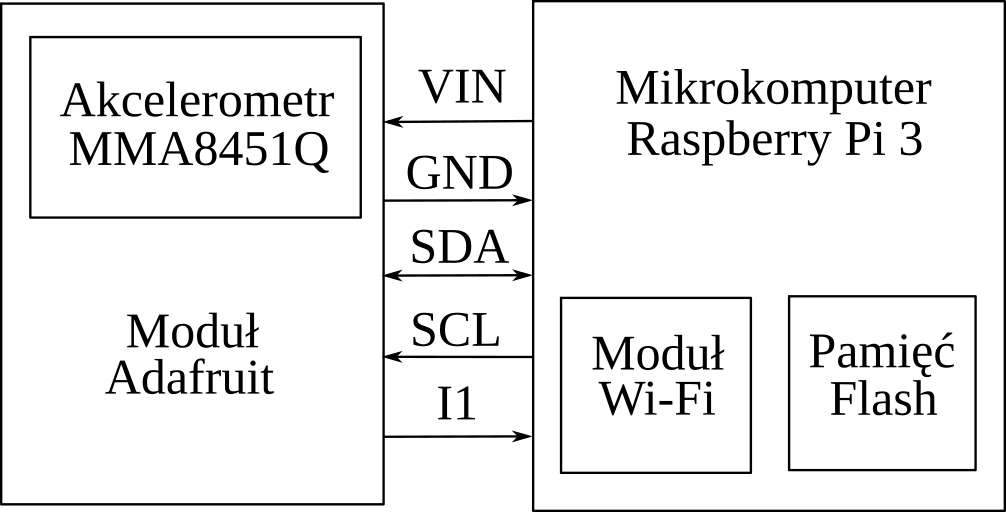
\includegraphics[width=0.8\textwidth]{bitgraphics/schemat_svg.png}',`
    \import{vecgraphics/}{schemat.pdf_tex}%')
  \caption{Schemat stworzonego systemu pomiarowego}
  \label{fig:schemat}
\end{figure}

Użyty do komunikacji z mikroprocesorem protokół I\textsuperscript{2}C jest
protokołem szeregowym oraz synchronicznym. Jego warstwa fizyczna składa się z
linii danych (SDA) oraz linii zegarowej (SCL). I\textsuperscript{2}C korzysta z
logiki odwróconej, a jego warstwa łącza danych oparta jest o system bajtowy. Po
przesłaniu 8-bitowej ramki danych następuje wysłanie bitu potwierdzającego
odbiór. Aby transmisja była możliwa konieczne jest zastosowanie rezystorów
podciągających do linii zasilania. Zostały one uwzględnione przez producenta
modułu akcelerometru i są umieszczone na płytce drukowanej. Dodatkowe dwie
linie to zasilanie modułu, którego napięcie, dzięki wewnętrznemu regulatorowi
napięcia, może zawierać się w przedziale od $+$\SI{3.3}{\volt} do
$+$\SI{5}{\volt} (VIN) oraz potencjał masy (GND).  Ostatnią linię stanowi linia
sygnału przerwania (I1), której działanie zostanie opisane później.

\begin{figure}[!tbh]
  \centering
  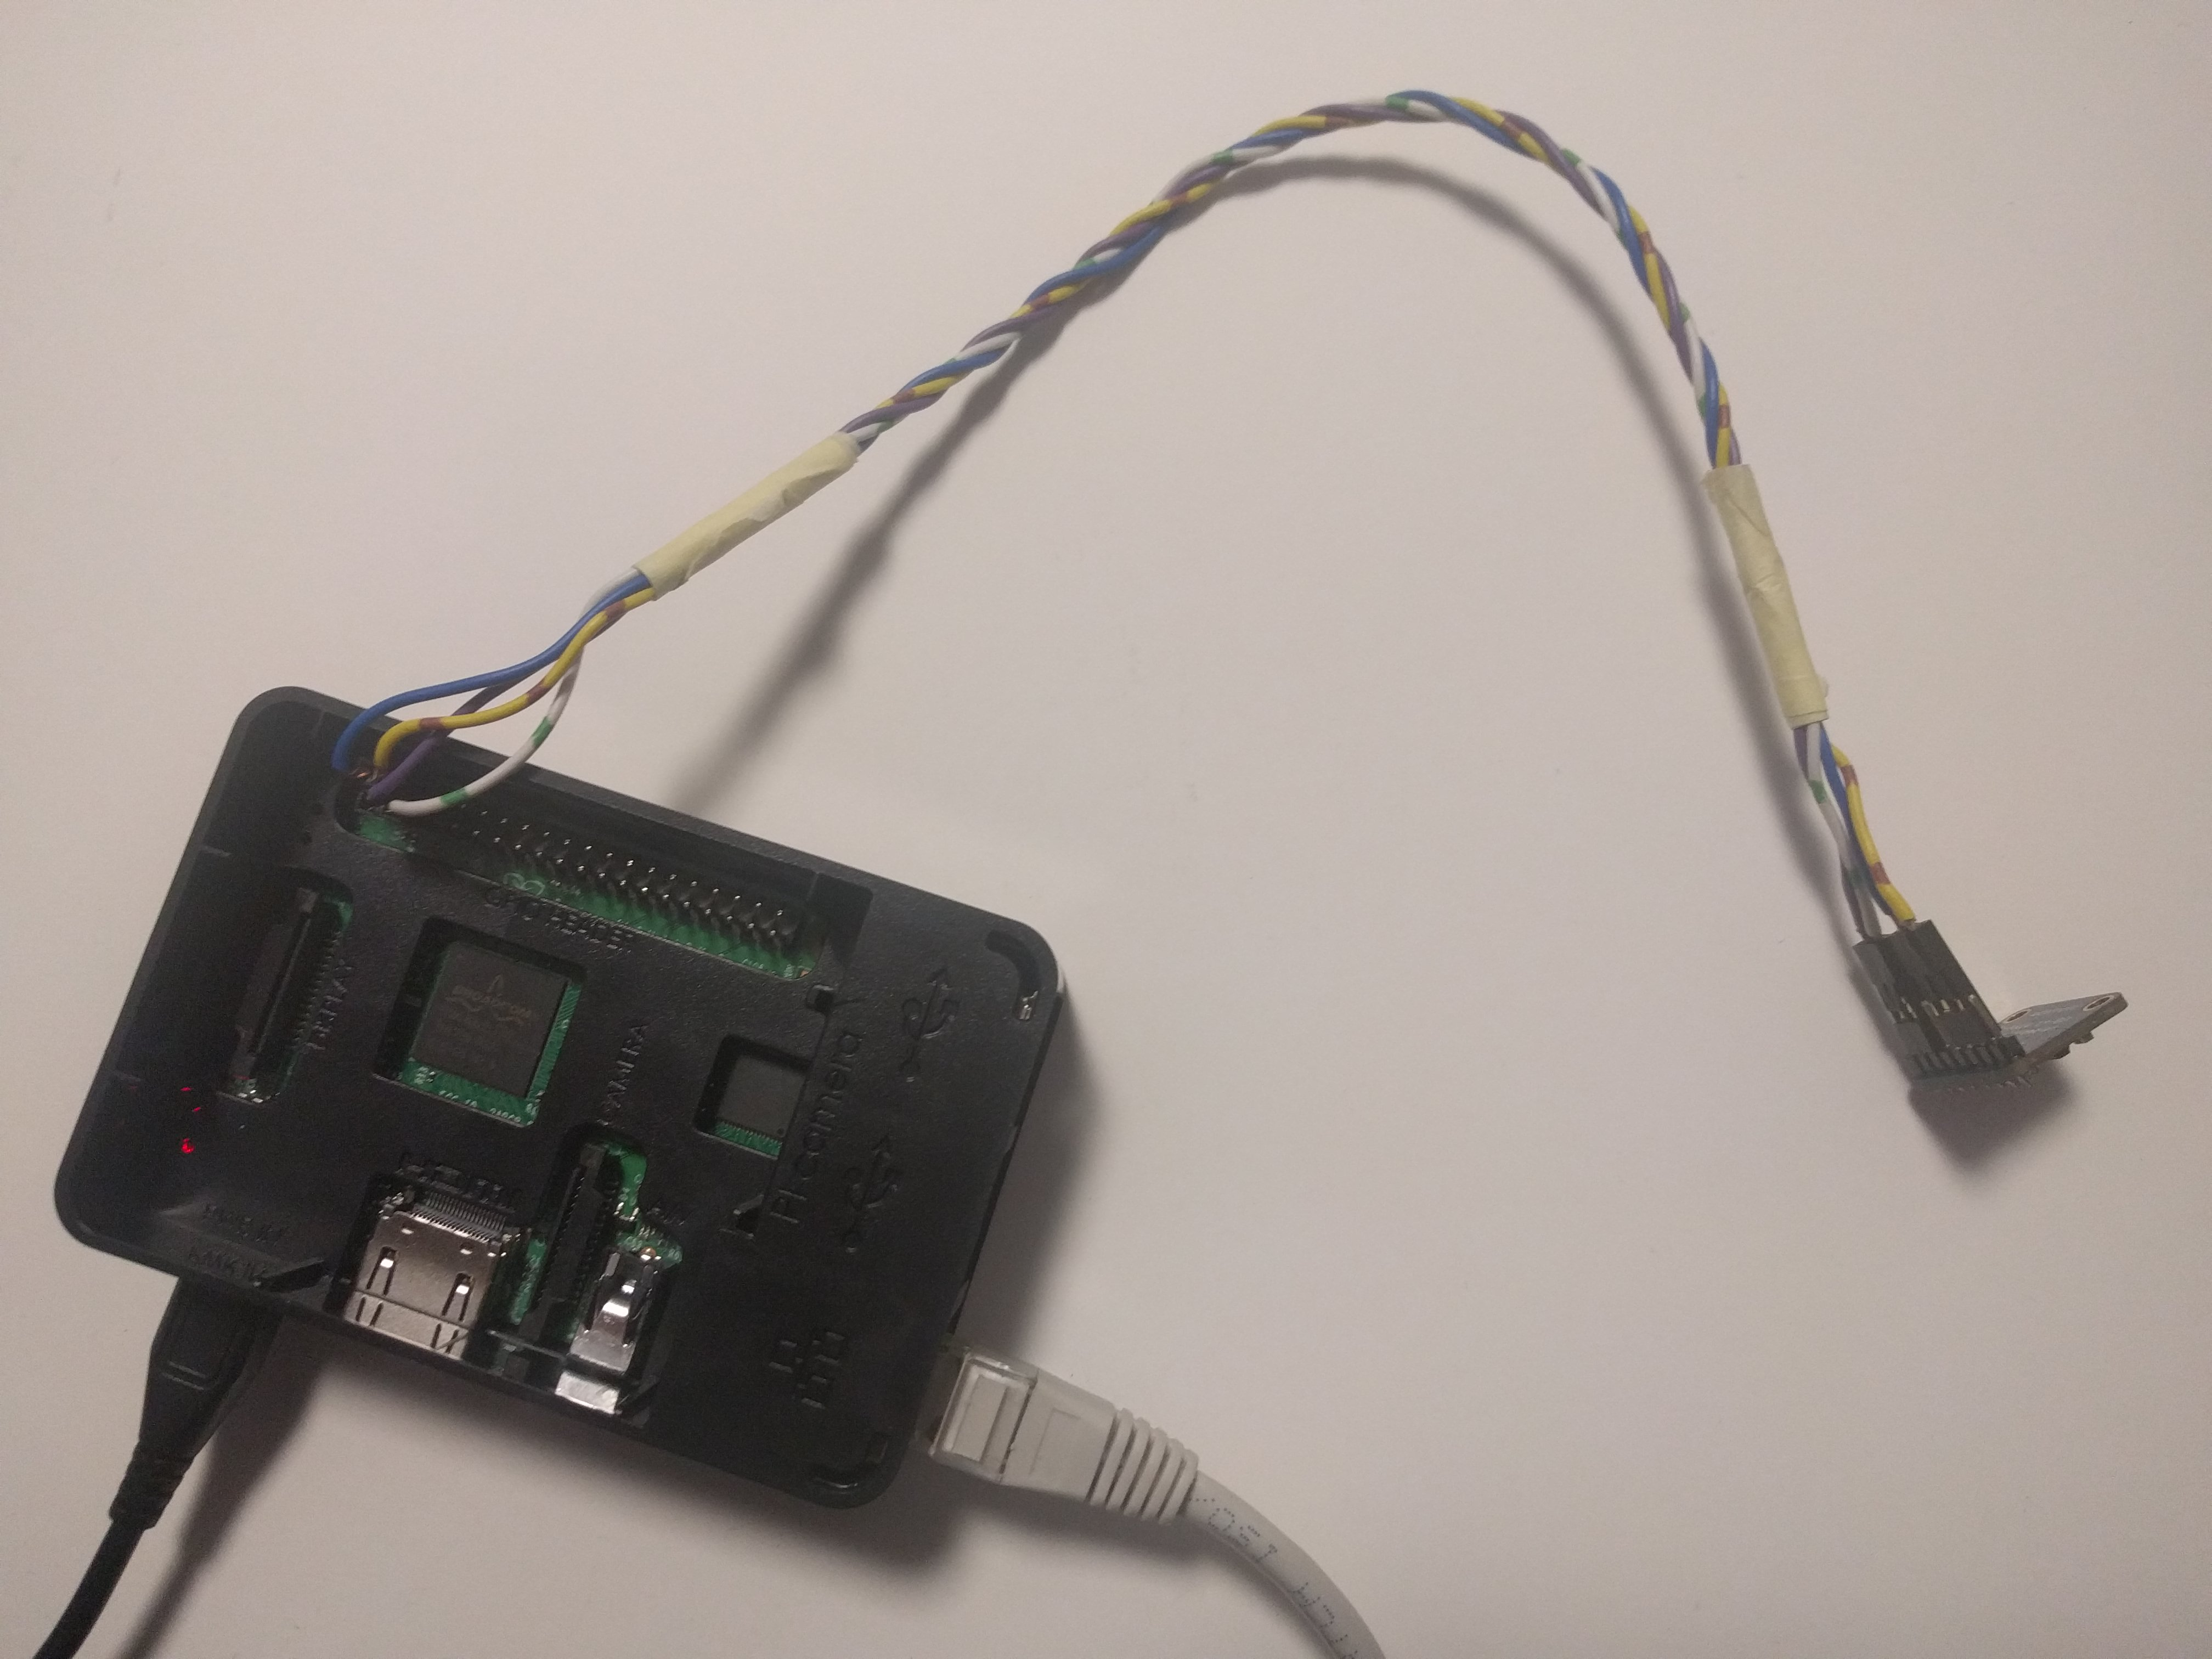
\includegraphics[width=\textwidth]{bitgraphics/pi.png}
  \caption{Wibroakustyczna stacja pomiarowa}
  \label{fig:foto}
\end{figure}

Od strony mikrokomputera Raspberry Pi obsługę wyżej wymienionych linii zapewnia
panel GPIO (General Purpose Input Output). Znajdują się w~nim piny zasilające,
uziemienia, piny dedykowanych do konkretnych protokołów komunikacji, w tym
I\textsuperscript{2}C, i piny których przeznaczenie nie jest ustalone.  Na
poziomie oprogramowania do obsługi komunikacji przez wybrany protokół pomocny
jest pakiet narzędzi {\fontfamily{\ttdefault}\selectfont i2c-tools}, który
między innymi pozwala odczytać adres urządzeń podłączonych do magistrali.

Główną częścią projektu było napisanie biblioteki do obsługi używanego
akcelerometru, oraz kodu który ją wykorzystuje w celu nieprzerwanej akwizycji i
zapisu danych pomiarowych. Dokładne działanie urządzenia zostało opisane w
dokumentacji \cite{mma8451}. Komunikacja z urządzeniem, przez protokół
I\textsuperscript{2}C, polegała na zapisie i odczycie danych z rejestrów.
Pierwszym krokiem było stworzenie części biblioteki która w wygodny sposób
pozwoli ustawiać flagi (kombinacje bitów w rejestrach, które sygnalizują
urządzeniu pożądaną konfigurację) i odczytywać dane z tych rejestrów. W tym
celu stworzono klasy \lstinline|Flag| i \lstinline|Register|, które
przechowują liczby odpowiadające odpowiednio kombinacji bitów flagi i
adresowi rejestru (Kod źr. \ref{code:reg}).

\begin{program}
  \caption{Definicja rejestru \lstinline|STATUS| i jego flag}
  \begin{lstlisting}
    import mma8451.register.addr as REG
    from mma8451.register.classes import Flag

    class STATUS(Flag):
      _addr           = REG.STATUS
      ZYXOW           = 0x80
      ZOW             = 0x40
      YOW             = 0x20
      XOW             = 0x10
      ZYXDR           = 0x08
      ZDR             = 0x04
      YDR             = 0x02
      XDR             = 0x01
  \end{lstlisting}
  \label{code:reg}
\end{program}

Następnie stworzono klasę \lstinline|IIC|, która, posiada metody pozwalające na
zapis wartości do rejestrów, jak i odczyt wartości przy wykorzystaniu uprzednio
stworzonych typów. Szczególnie ważne było stworzenie metody pozyskiwania
wartości w trybie \emph{burst}, który pozwala na odczyt wielu wartości naraz
jednym ciągiem danych. Wykorzystuje ona bibliotekę \emph{pigpio}~\cite{pigpio}.

\begin{program}
  \caption{Wykorzystanie klasy IIC do poboru danych}
  \begin{lstlisting}
    from mma8451.register import register as REG
    from mma8451.iic import IIC
    import pigpio

    # Inicjalizacja połączenia z procesem pigpio
    pi = pigpio.pi()
    # Stwórz obiekt klasy, gdzie 1 do magistrala a 0x1D adres
    iic = IIC(pi, 1, 0x1D)
    # Uśpij urządzenie
    iic.unset_flag(REG.CTRL_REG1.ACTIVE)
    # Włącz tryb 14-to bitowy
    iic.unset_flag(REG.CTRL_REG1.F_READ)
    # Włacz urządzenie do trybu aktywnego
    iic.set_flag(REG.CTRL_REG1.ACTIVE)
    # Pobierz dane ze wszystkich trzech osi
    dane = iic.block_read(REG.OUT_X_MSB, 6)
  \end{lstlisting}
  \label{code:iic}
\end{program}

Po napisaniu tych elementów biblioteki zajęto się jej główną częścią, służącą
do inicjalizacji urządzenia, obsługi przerwań, ustawienia pożądanych parametrów
i przygotowania wątków i procesów ciągłej akwizycji i zapisu danych. W procesie
inicializacji ustawiane są flagi włączające tryb niskoszumowy urządzenia oraz
najmniej energooszczędny, natomiast najbardziej dokładny tryb próbkowania.
Ustawienia zakresu dynamicznego oraz częstotliwości próbkowania pozostawione są
na swoich domyślnych wartościach, odpowiednio $\pm\SI{2}{\g}$ oraz
\SI{800}{\hertz}. Pozwala to zapewnić maksymalną dokładność uzyskanych z
urządzenia danych.

Kolejno ustawiane są flagi które aktywują wbudowaną kolejkę FIFO (First In
First Out) urządzenia. Aby nie stracić żadnych próbek z powodu tymczasowego
spowolnienia wykonywania programu oraz by nie zajmować całego czasu procesora
poprzez ciągłe sprawdzanie rejestrów w oczekiwaniu na nowe próbki, jest
wykorzystana ta kolejka, która może przechowywać aż do trzydziestu dwóch
czternasto-bitowych próbek z trzech osi. Kolejka jest ustawiana tak, by w
momencie wykroczenia liczby próbek w kolejce ponad dwadzieścia następowało
przerwanie, wysyłane w postaci zmiany stanu na pinie \emph{I1} do GPIO.
W programie ustawiona jest by w momencie wykrycia tej zmiany została wykonana
funkcja, która informuje wątek akwizycji o dostępności nowych danych.

Po inicjalizacji ustawień uruchamiany jest wątek akwizycji danych oraz proces,
który się zajmuje ich zapisywaniem. Wątek akwizycji czeka na informację o
dostępności nowych danych po czym odczytuje wszystkie próbki z~kolejki
wykorzystując do tego wspomniany wcześniej tryb \emph{burst}, a następnie
zebrane wartości przekazuje do kolejki. Na dane w kolejce czeka proces
zapisujący, który po zebraniu odpowiedniej liczby próbek, która w tym momencie
odpowiada pięciu minutom, przeprowadza zamianę uzyskanych wartości z~kodu
uzupełnień do dwóch na liczbę całkowitą ze znakiem, po czym uzyskaną macierz
zawierającą dane ze wszystkich osi zapisuje do pliku HDF5 w grupach
odpowiadających dacie i godzinie zapisu. Wybrano format HDF5 z powodu na jego
uniwersalność oraz wewnętrzną strukturę (Rys. \ref{fig:struc}).

\begin{figure}[!tbh]%
  \centering%
  %m4_ifodt(`
  %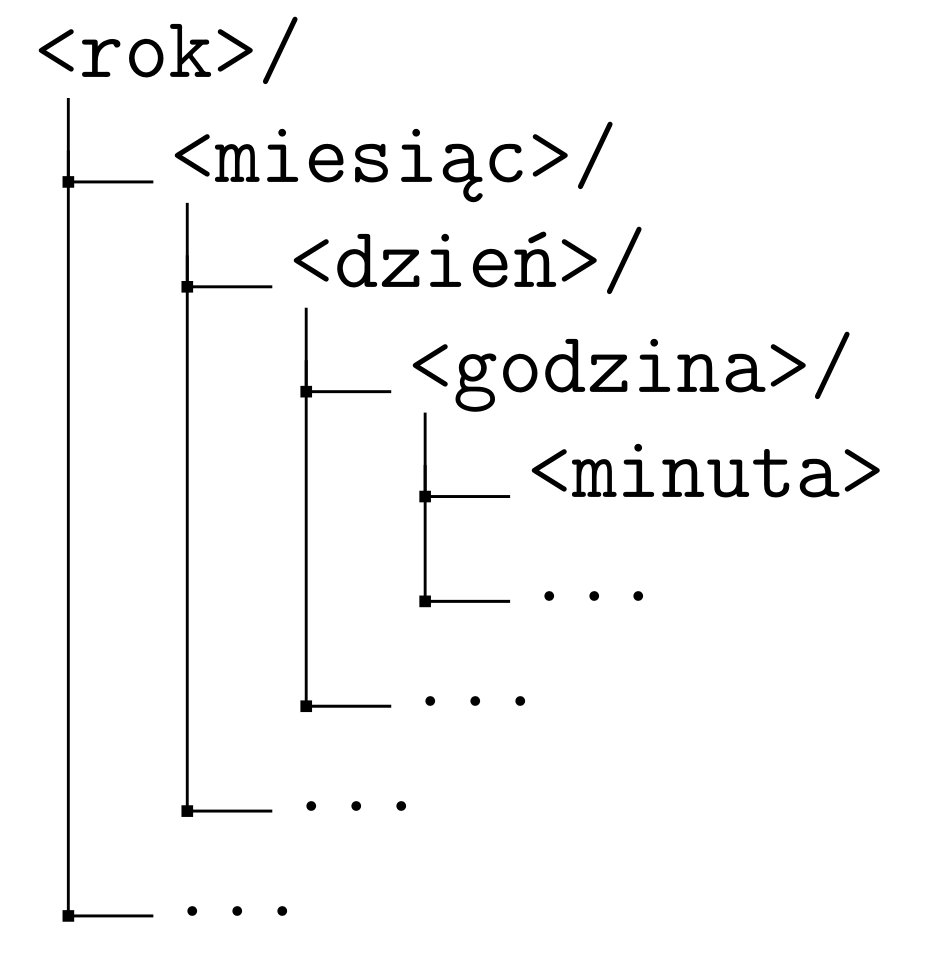
\includegraphics[width=0.8\textwidth]{bitgraphics/struktura.png}',`
  \begin{minipage}{0.3\textwidth}%
    \dirtree{%
      .1 <rok>/.
      .2 <miesiąc>/.
      .3 <dzień>/.
      .4 <godzina>/.
      .5 <minuta>.
      .5 \dots.
      .4 \dots.
      .3 \dots.
      .2 \dots.
    }%
  \end{minipage}%')
  \caption{Struktura grup w pliku z danymi}%
  \label{fig:struc}%
\end{figure}%

Stacja pomiarowa jest zdolna do zapisania w swojej pamięci wewnętrznej około
miesiąca wibrogramu. Ponieważ norma wymaga analizy tercjowej drgań, uwzględniono
filtrację sygnału w pasmach od \SI{0,5}{\hertz} do \SI{100}{\hertz}. W~celu
weryfikacji działania stacji umieszczono ją w budynku D1 należącym do Katedry
Mechaniki i Wibroakustyki AGH oraz uruchomiono na 18 godzin. Zdjęcia
\ref{fig:pomiar1} oraz \ref{fig:imadlo} przedstawiają stację ustawioną do
pomiaru. W dalszej perspektywie planowane jest zaprojektowanie i wytworzenie
dedykowanych dla modułów akcelerometrów obudów. Na potrzeby testów działania
akcelerometr został przytwierdzony do imadła, a następnie do bloków stalowych o
dużej masie, zapewniających jego stabilność podczas rejestracji danych. Wartości
przyspieszenia mierzone były na parapecie w bezpośredniej bliskości belek
konstrukcyjnych znajdujących się w podpiwniczeniu budynku.

\begin{figure}[!tbh]
  \centering
  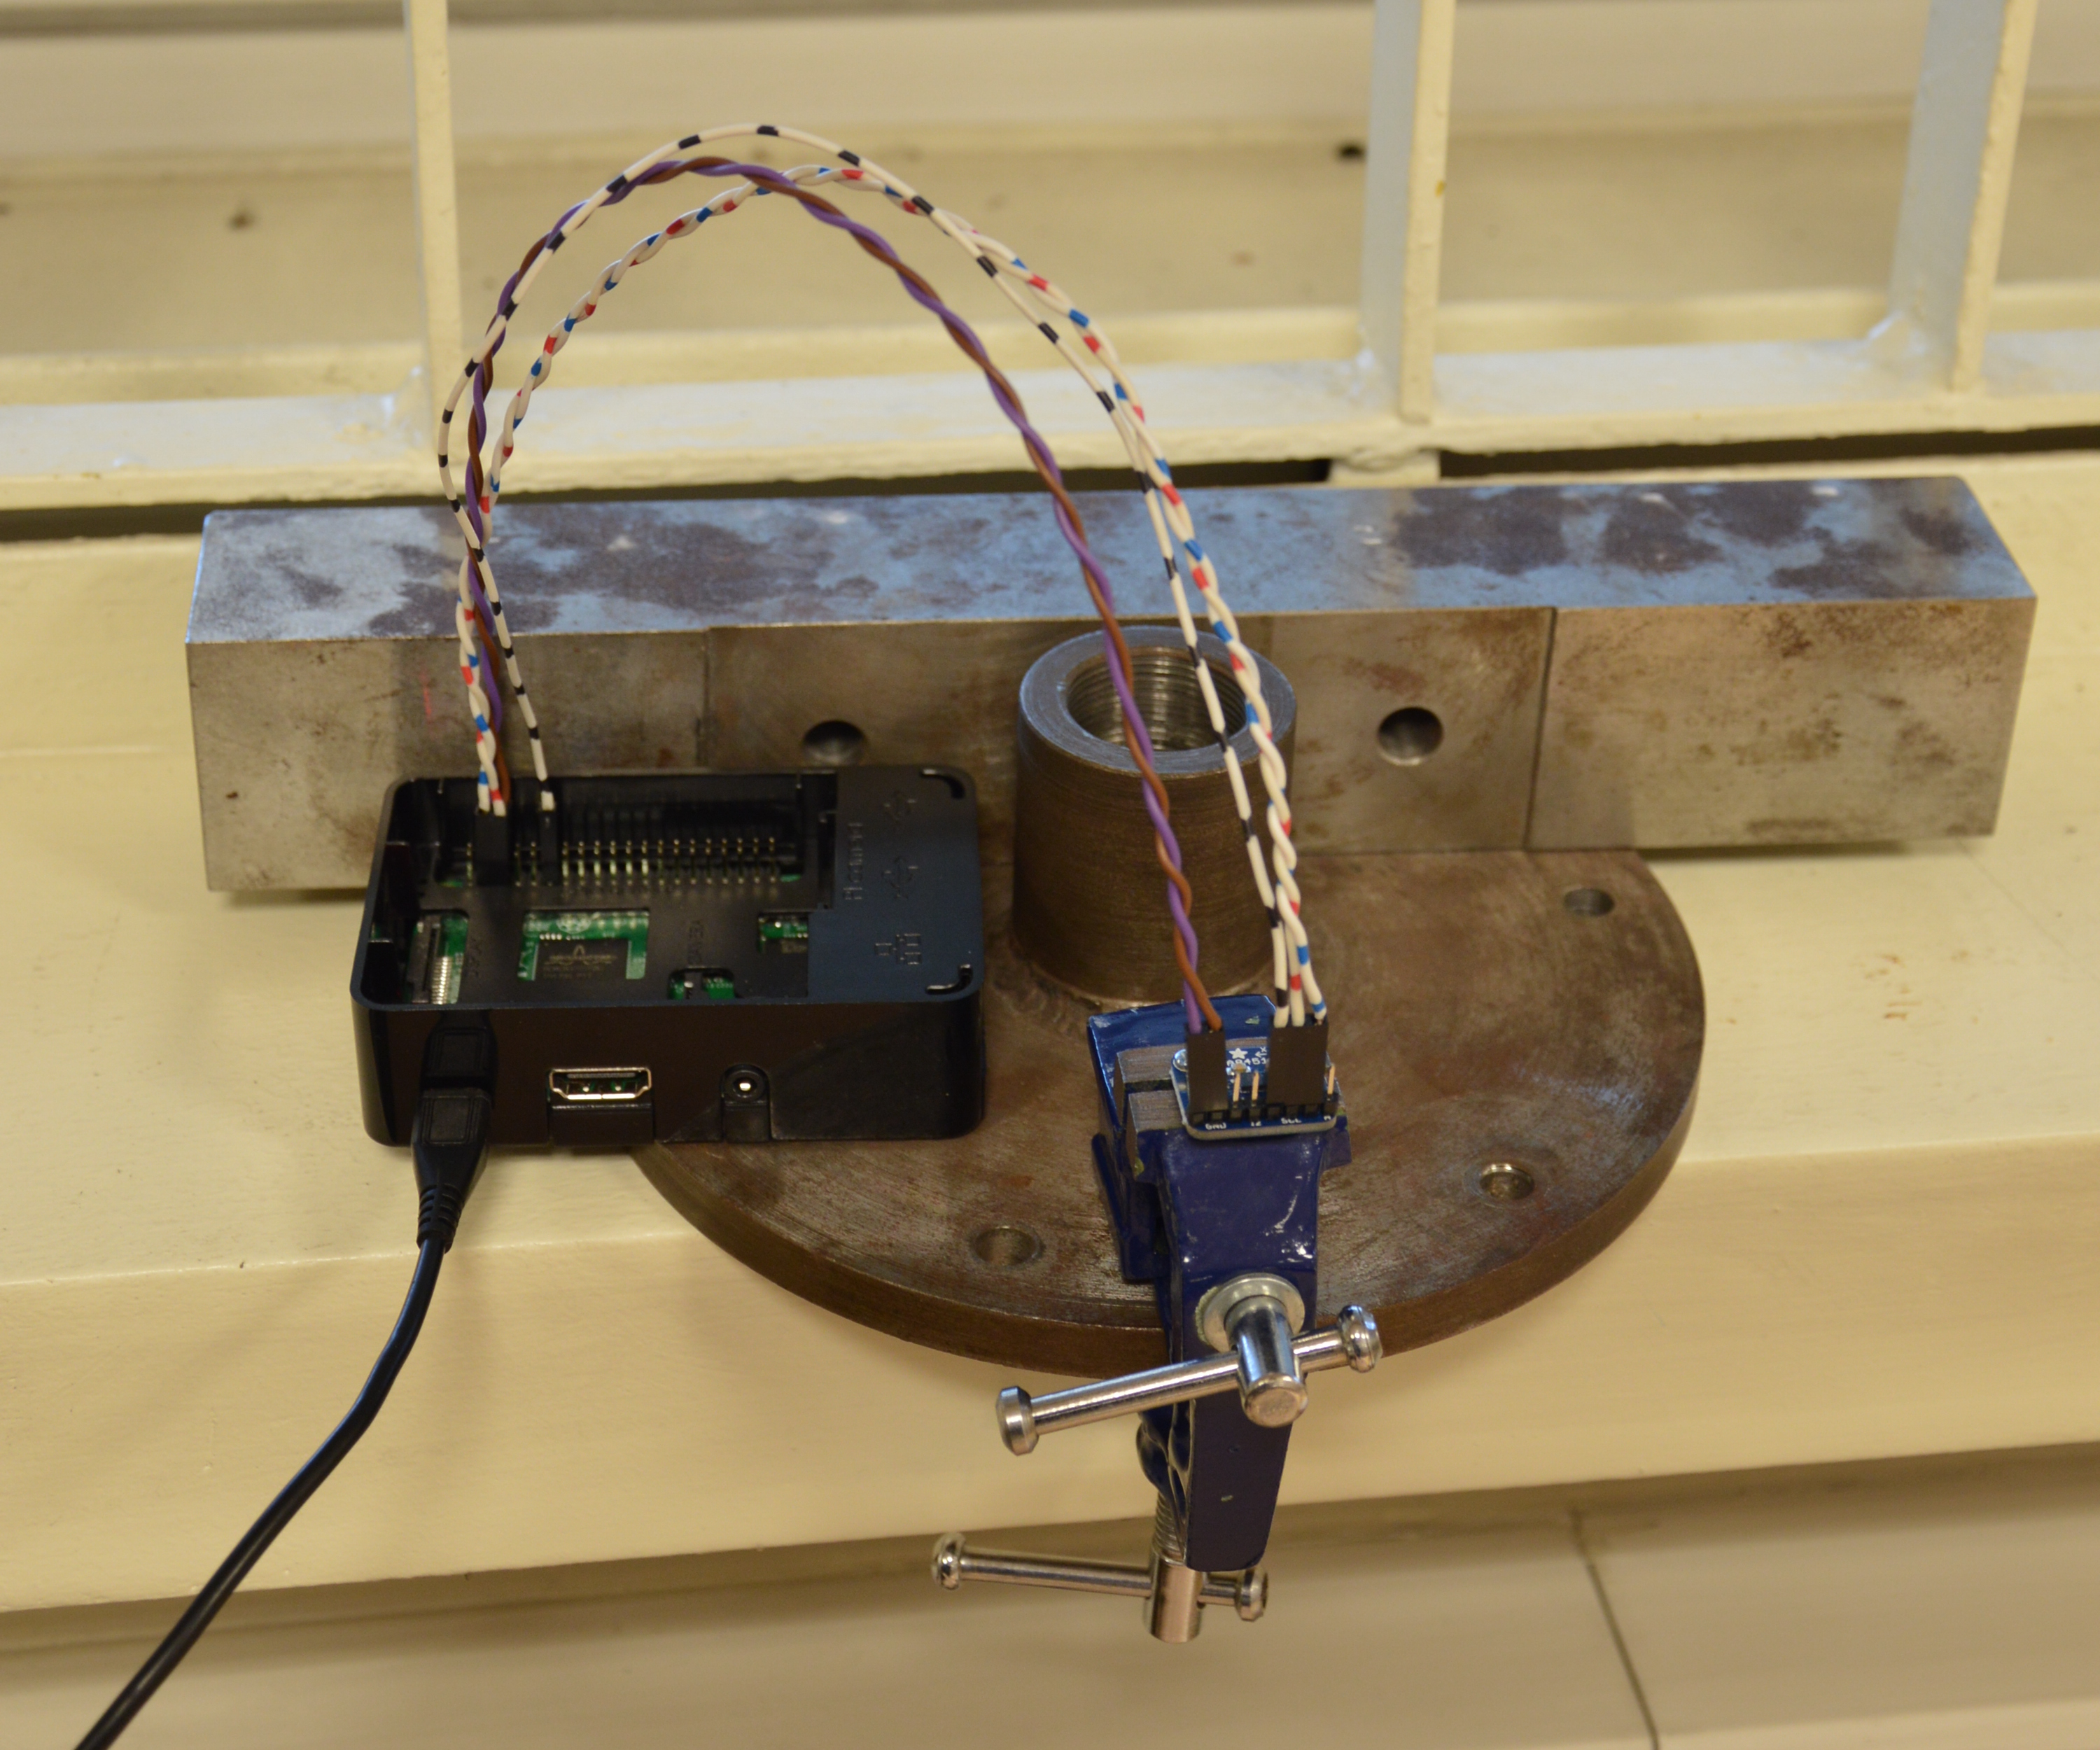
\includegraphics[width=0.8\textwidth]{bitgraphics/pom_2_cut.jpg}
  \caption{Stacja pomiarowa podczas pracy}
  \label{fig:pomiar1}
\end{figure}

\begin{figure}[!tbh]
  \centering
  \includegraphics[width=0.8\textwidth]{bitgraphics/pom_1.jpg}
  \caption{Tymczasowe mocowanie akcelerometru}
  \label{fig:imadlo}
\end{figure}

Wykresy \ref{plot:accel_x} oraz \ref{plot:power_x} pokazują wyniki pomiaru
testowego. Przedstawiono fragment wibrogramu przyspieszenia drgań dla osi X
(zorientowanej na kierunku pionowym, przeciwnie do kierunku przyspieszenia
ziemskiego podczas pomiaru). Dodatkowo, pokazano widmo amplitudowe sygnału
zarejestrowanego między godziną 7:00, a 8:00 rano (kiedy ruch samochodowy na
pobliskiej ulicy jest największy).

Jak można zauważyć na poniższych wykresach, rejestrowany sygnał jest
prawdopodobnie pochodzenia szumowego, o losowym charakterze. Wskazuje na to
płaska charakterystyka widma amplitudowego. Wynika z tego, że drgania badanego
budynku mają na tyle małą amplitudę, że ich sygnał jest maskowany szumem
wprowadzonym przez sam przetwornik oraz tor pomiarowy.

\begin{figure}[!tbh]
  \centering
  %m4_ifodt(`
  % 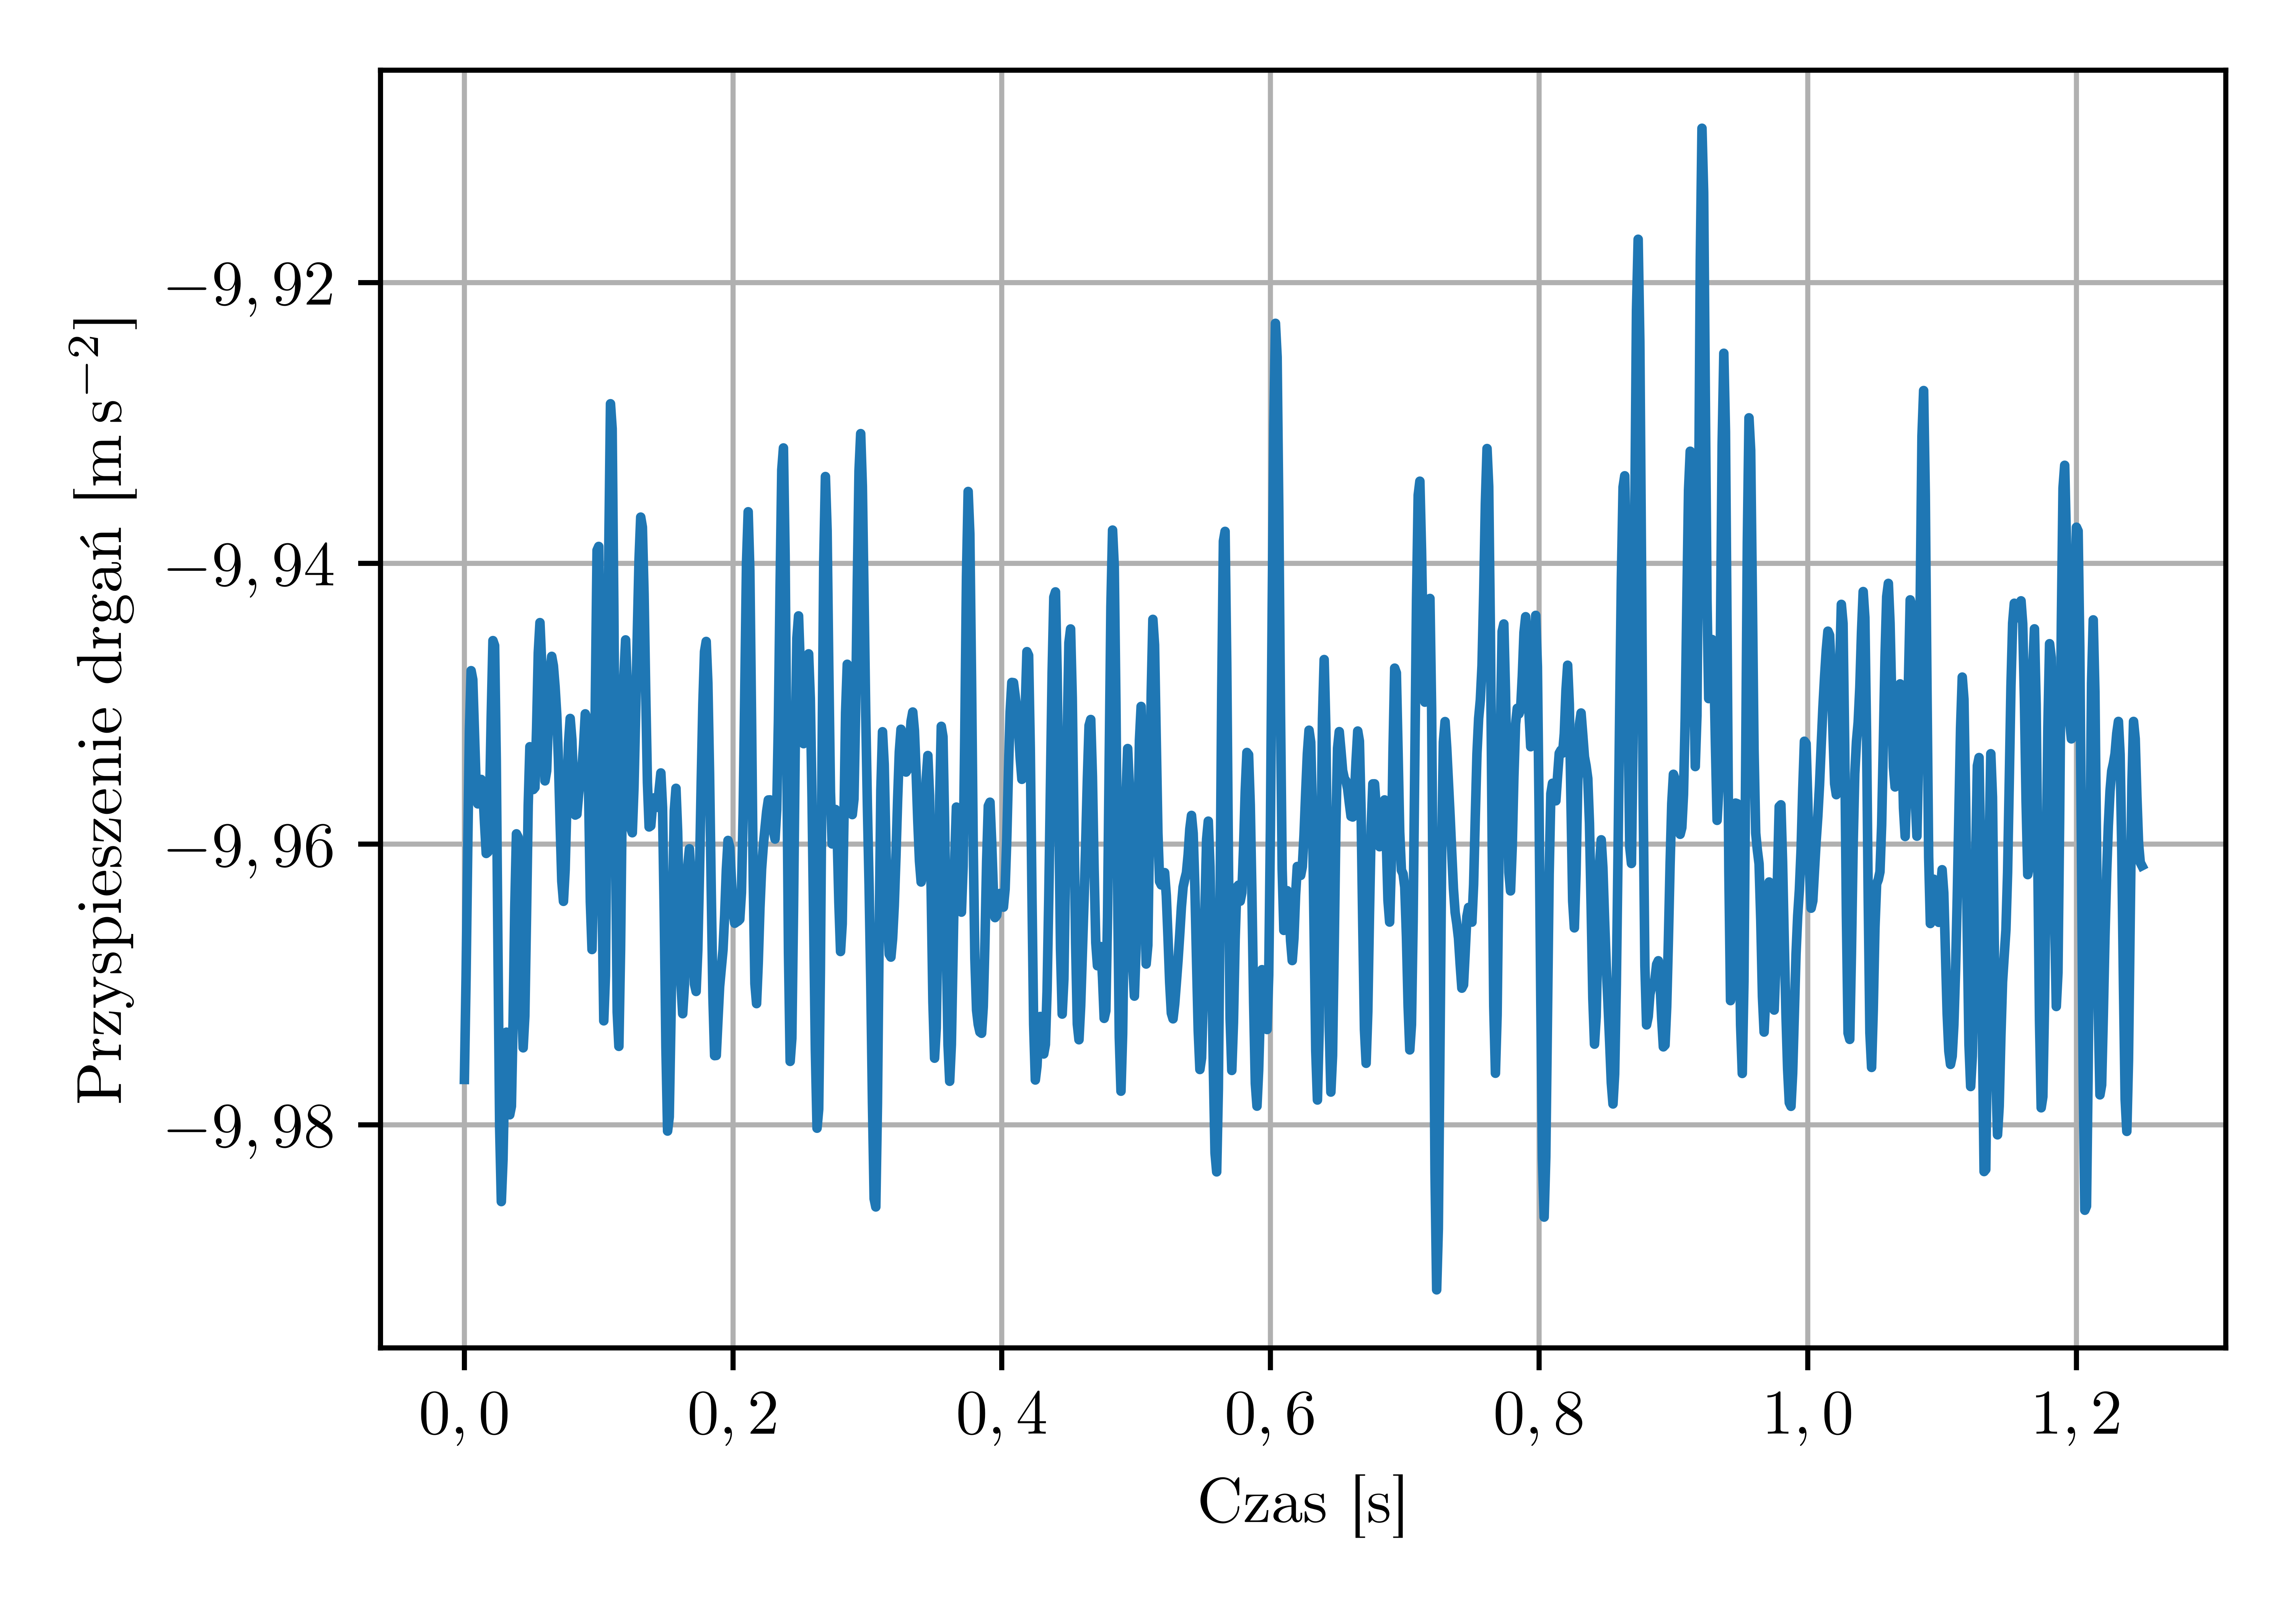
\includegraphics[width=0.8\textwidth]{plots/accel_x.png}',`
    %% Creator: Matplotlib, PGF backend
%%
%% To include the figure in your LaTeX document, write
%%   \input{<filename>.pgf}
%%
%% Make sure the required packages are loaded in your preamble
%%   \usepackage{pgf}
%%
%% Figures using additional raster images can only be included by \input if
%% they are in the same directory as the main LaTeX file. For loading figures
%% from other directories you can use the `import` package
%%   \usepackage{import}
%% and then include the figures with
%%   \import{<path to file>}{<filename>.pgf}
%%
%% Matplotlib used the following preamble
%%   \usepackage[utf8]{inputenc}
%%   \usepackage[T1]{fontenc}
%%   \usepackage{siunitx}
%%
\begingroup%
\makeatletter%
\begin{pgfpicture}%
\pgfpathrectangle{\pgfpointorigin}{\pgfqpoint{5.000000in}{3.500000in}}%
\pgfusepath{use as bounding box, clip}%
\begin{pgfscope}%
\pgfsetbuttcap%
\pgfsetmiterjoin%
\definecolor{currentfill}{rgb}{1.000000,1.000000,1.000000}%
\pgfsetfillcolor{currentfill}%
\pgfsetlinewidth{0.000000pt}%
\definecolor{currentstroke}{rgb}{1.000000,1.000000,1.000000}%
\pgfsetstrokecolor{currentstroke}%
\pgfsetdash{}{0pt}%
\pgfpathmoveto{\pgfqpoint{0.000000in}{0.000000in}}%
\pgfpathlineto{\pgfqpoint{5.000000in}{0.000000in}}%
\pgfpathlineto{\pgfqpoint{5.000000in}{3.500000in}}%
\pgfpathlineto{\pgfqpoint{0.000000in}{3.500000in}}%
\pgfpathclose%
\pgfusepath{fill}%
\end{pgfscope}%
\begin{pgfscope}%
\pgfsetbuttcap%
\pgfsetmiterjoin%
\definecolor{currentfill}{rgb}{1.000000,1.000000,1.000000}%
\pgfsetfillcolor{currentfill}%
\pgfsetlinewidth{0.000000pt}%
\definecolor{currentstroke}{rgb}{0.000000,0.000000,0.000000}%
\pgfsetstrokecolor{currentstroke}%
\pgfsetstrokeopacity{0.000000}%
\pgfsetdash{}{0pt}%
\pgfpathmoveto{\pgfqpoint{0.967524in}{0.564288in}}%
\pgfpathlineto{\pgfqpoint{4.815000in}{0.564288in}}%
\pgfpathlineto{\pgfqpoint{4.815000in}{3.315000in}}%
\pgfpathlineto{\pgfqpoint{0.967524in}{3.315000in}}%
\pgfpathclose%
\pgfusepath{fill}%
\end{pgfscope}%
\begin{pgfscope}%
\pgfpathrectangle{\pgfqpoint{0.967524in}{0.564288in}}{\pgfqpoint{3.847476in}{2.750712in}}%
\pgfusepath{clip}%
\pgfsetrectcap%
\pgfsetroundjoin%
\pgfsetlinewidth{0.803000pt}%
\definecolor{currentstroke}{rgb}{0.690196,0.690196,0.690196}%
\pgfsetstrokecolor{currentstroke}%
\pgfsetdash{}{0pt}%
\pgfpathmoveto{\pgfqpoint{1.142409in}{0.564288in}}%
\pgfpathlineto{\pgfqpoint{1.142409in}{3.315000in}}%
\pgfusepath{stroke}%
\end{pgfscope}%
\begin{pgfscope}%
\pgfsetbuttcap%
\pgfsetroundjoin%
\definecolor{currentfill}{rgb}{0.000000,0.000000,0.000000}%
\pgfsetfillcolor{currentfill}%
\pgfsetlinewidth{0.803000pt}%
\definecolor{currentstroke}{rgb}{0.000000,0.000000,0.000000}%
\pgfsetstrokecolor{currentstroke}%
\pgfsetdash{}{0pt}%
\pgfsys@defobject{currentmarker}{\pgfqpoint{0.000000in}{-0.048611in}}{\pgfqpoint{0.000000in}{0.000000in}}{%
\pgfpathmoveto{\pgfqpoint{0.000000in}{0.000000in}}%
\pgfpathlineto{\pgfqpoint{0.000000in}{-0.048611in}}%
\pgfusepath{stroke,fill}%
}%
\begin{pgfscope}%
\pgfsys@transformshift{1.142409in}{0.564288in}%
\pgfsys@useobject{currentmarker}{}%
\end{pgfscope}%
\end{pgfscope}%
\begin{pgfscope}%
\pgftext[x=1.142409in,y=0.467066in,,top]{\rmfamily\fontsize{10.000000}{12.000000}\selectfont \(\displaystyle 0,0\)}%
\end{pgfscope}%
\begin{pgfscope}%
\pgfpathrectangle{\pgfqpoint{0.967524in}{0.564288in}}{\pgfqpoint{3.847476in}{2.750712in}}%
\pgfusepath{clip}%
\pgfsetrectcap%
\pgfsetroundjoin%
\pgfsetlinewidth{0.803000pt}%
\definecolor{currentstroke}{rgb}{0.690196,0.690196,0.690196}%
\pgfsetstrokecolor{currentstroke}%
\pgfsetdash{}{0pt}%
\pgfpathmoveto{\pgfqpoint{1.702602in}{0.564288in}}%
\pgfpathlineto{\pgfqpoint{1.702602in}{3.315000in}}%
\pgfusepath{stroke}%
\end{pgfscope}%
\begin{pgfscope}%
\pgfsetbuttcap%
\pgfsetroundjoin%
\definecolor{currentfill}{rgb}{0.000000,0.000000,0.000000}%
\pgfsetfillcolor{currentfill}%
\pgfsetlinewidth{0.803000pt}%
\definecolor{currentstroke}{rgb}{0.000000,0.000000,0.000000}%
\pgfsetstrokecolor{currentstroke}%
\pgfsetdash{}{0pt}%
\pgfsys@defobject{currentmarker}{\pgfqpoint{0.000000in}{-0.048611in}}{\pgfqpoint{0.000000in}{0.000000in}}{%
\pgfpathmoveto{\pgfqpoint{0.000000in}{0.000000in}}%
\pgfpathlineto{\pgfqpoint{0.000000in}{-0.048611in}}%
\pgfusepath{stroke,fill}%
}%
\begin{pgfscope}%
\pgfsys@transformshift{1.702602in}{0.564288in}%
\pgfsys@useobject{currentmarker}{}%
\end{pgfscope}%
\end{pgfscope}%
\begin{pgfscope}%
\pgftext[x=1.702602in,y=0.467066in,,top]{\rmfamily\fontsize{10.000000}{12.000000}\selectfont \(\displaystyle 0,2\)}%
\end{pgfscope}%
\begin{pgfscope}%
\pgfpathrectangle{\pgfqpoint{0.967524in}{0.564288in}}{\pgfqpoint{3.847476in}{2.750712in}}%
\pgfusepath{clip}%
\pgfsetrectcap%
\pgfsetroundjoin%
\pgfsetlinewidth{0.803000pt}%
\definecolor{currentstroke}{rgb}{0.690196,0.690196,0.690196}%
\pgfsetstrokecolor{currentstroke}%
\pgfsetdash{}{0pt}%
\pgfpathmoveto{\pgfqpoint{2.262795in}{0.564288in}}%
\pgfpathlineto{\pgfqpoint{2.262795in}{3.315000in}}%
\pgfusepath{stroke}%
\end{pgfscope}%
\begin{pgfscope}%
\pgfsetbuttcap%
\pgfsetroundjoin%
\definecolor{currentfill}{rgb}{0.000000,0.000000,0.000000}%
\pgfsetfillcolor{currentfill}%
\pgfsetlinewidth{0.803000pt}%
\definecolor{currentstroke}{rgb}{0.000000,0.000000,0.000000}%
\pgfsetstrokecolor{currentstroke}%
\pgfsetdash{}{0pt}%
\pgfsys@defobject{currentmarker}{\pgfqpoint{0.000000in}{-0.048611in}}{\pgfqpoint{0.000000in}{0.000000in}}{%
\pgfpathmoveto{\pgfqpoint{0.000000in}{0.000000in}}%
\pgfpathlineto{\pgfqpoint{0.000000in}{-0.048611in}}%
\pgfusepath{stroke,fill}%
}%
\begin{pgfscope}%
\pgfsys@transformshift{2.262795in}{0.564288in}%
\pgfsys@useobject{currentmarker}{}%
\end{pgfscope}%
\end{pgfscope}%
\begin{pgfscope}%
\pgftext[x=2.262795in,y=0.467066in,,top]{\rmfamily\fontsize{10.000000}{12.000000}\selectfont \(\displaystyle 0,4\)}%
\end{pgfscope}%
\begin{pgfscope}%
\pgfpathrectangle{\pgfqpoint{0.967524in}{0.564288in}}{\pgfqpoint{3.847476in}{2.750712in}}%
\pgfusepath{clip}%
\pgfsetrectcap%
\pgfsetroundjoin%
\pgfsetlinewidth{0.803000pt}%
\definecolor{currentstroke}{rgb}{0.690196,0.690196,0.690196}%
\pgfsetstrokecolor{currentstroke}%
\pgfsetdash{}{0pt}%
\pgfpathmoveto{\pgfqpoint{2.822988in}{0.564288in}}%
\pgfpathlineto{\pgfqpoint{2.822988in}{3.315000in}}%
\pgfusepath{stroke}%
\end{pgfscope}%
\begin{pgfscope}%
\pgfsetbuttcap%
\pgfsetroundjoin%
\definecolor{currentfill}{rgb}{0.000000,0.000000,0.000000}%
\pgfsetfillcolor{currentfill}%
\pgfsetlinewidth{0.803000pt}%
\definecolor{currentstroke}{rgb}{0.000000,0.000000,0.000000}%
\pgfsetstrokecolor{currentstroke}%
\pgfsetdash{}{0pt}%
\pgfsys@defobject{currentmarker}{\pgfqpoint{0.000000in}{-0.048611in}}{\pgfqpoint{0.000000in}{0.000000in}}{%
\pgfpathmoveto{\pgfqpoint{0.000000in}{0.000000in}}%
\pgfpathlineto{\pgfqpoint{0.000000in}{-0.048611in}}%
\pgfusepath{stroke,fill}%
}%
\begin{pgfscope}%
\pgfsys@transformshift{2.822988in}{0.564288in}%
\pgfsys@useobject{currentmarker}{}%
\end{pgfscope}%
\end{pgfscope}%
\begin{pgfscope}%
\pgftext[x=2.822988in,y=0.467066in,,top]{\rmfamily\fontsize{10.000000}{12.000000}\selectfont \(\displaystyle 0,6\)}%
\end{pgfscope}%
\begin{pgfscope}%
\pgfpathrectangle{\pgfqpoint{0.967524in}{0.564288in}}{\pgfqpoint{3.847476in}{2.750712in}}%
\pgfusepath{clip}%
\pgfsetrectcap%
\pgfsetroundjoin%
\pgfsetlinewidth{0.803000pt}%
\definecolor{currentstroke}{rgb}{0.690196,0.690196,0.690196}%
\pgfsetstrokecolor{currentstroke}%
\pgfsetdash{}{0pt}%
\pgfpathmoveto{\pgfqpoint{3.383181in}{0.564288in}}%
\pgfpathlineto{\pgfqpoint{3.383181in}{3.315000in}}%
\pgfusepath{stroke}%
\end{pgfscope}%
\begin{pgfscope}%
\pgfsetbuttcap%
\pgfsetroundjoin%
\definecolor{currentfill}{rgb}{0.000000,0.000000,0.000000}%
\pgfsetfillcolor{currentfill}%
\pgfsetlinewidth{0.803000pt}%
\definecolor{currentstroke}{rgb}{0.000000,0.000000,0.000000}%
\pgfsetstrokecolor{currentstroke}%
\pgfsetdash{}{0pt}%
\pgfsys@defobject{currentmarker}{\pgfqpoint{0.000000in}{-0.048611in}}{\pgfqpoint{0.000000in}{0.000000in}}{%
\pgfpathmoveto{\pgfqpoint{0.000000in}{0.000000in}}%
\pgfpathlineto{\pgfqpoint{0.000000in}{-0.048611in}}%
\pgfusepath{stroke,fill}%
}%
\begin{pgfscope}%
\pgfsys@transformshift{3.383181in}{0.564288in}%
\pgfsys@useobject{currentmarker}{}%
\end{pgfscope}%
\end{pgfscope}%
\begin{pgfscope}%
\pgftext[x=3.383181in,y=0.467066in,,top]{\rmfamily\fontsize{10.000000}{12.000000}\selectfont \(\displaystyle 0,8\)}%
\end{pgfscope}%
\begin{pgfscope}%
\pgfpathrectangle{\pgfqpoint{0.967524in}{0.564288in}}{\pgfqpoint{3.847476in}{2.750712in}}%
\pgfusepath{clip}%
\pgfsetrectcap%
\pgfsetroundjoin%
\pgfsetlinewidth{0.803000pt}%
\definecolor{currentstroke}{rgb}{0.690196,0.690196,0.690196}%
\pgfsetstrokecolor{currentstroke}%
\pgfsetdash{}{0pt}%
\pgfpathmoveto{\pgfqpoint{3.943375in}{0.564288in}}%
\pgfpathlineto{\pgfqpoint{3.943375in}{3.315000in}}%
\pgfusepath{stroke}%
\end{pgfscope}%
\begin{pgfscope}%
\pgfsetbuttcap%
\pgfsetroundjoin%
\definecolor{currentfill}{rgb}{0.000000,0.000000,0.000000}%
\pgfsetfillcolor{currentfill}%
\pgfsetlinewidth{0.803000pt}%
\definecolor{currentstroke}{rgb}{0.000000,0.000000,0.000000}%
\pgfsetstrokecolor{currentstroke}%
\pgfsetdash{}{0pt}%
\pgfsys@defobject{currentmarker}{\pgfqpoint{0.000000in}{-0.048611in}}{\pgfqpoint{0.000000in}{0.000000in}}{%
\pgfpathmoveto{\pgfqpoint{0.000000in}{0.000000in}}%
\pgfpathlineto{\pgfqpoint{0.000000in}{-0.048611in}}%
\pgfusepath{stroke,fill}%
}%
\begin{pgfscope}%
\pgfsys@transformshift{3.943375in}{0.564288in}%
\pgfsys@useobject{currentmarker}{}%
\end{pgfscope}%
\end{pgfscope}%
\begin{pgfscope}%
\pgftext[x=3.943375in,y=0.467066in,,top]{\rmfamily\fontsize{10.000000}{12.000000}\selectfont \(\displaystyle 1,0\)}%
\end{pgfscope}%
\begin{pgfscope}%
\pgfpathrectangle{\pgfqpoint{0.967524in}{0.564288in}}{\pgfqpoint{3.847476in}{2.750712in}}%
\pgfusepath{clip}%
\pgfsetrectcap%
\pgfsetroundjoin%
\pgfsetlinewidth{0.803000pt}%
\definecolor{currentstroke}{rgb}{0.690196,0.690196,0.690196}%
\pgfsetstrokecolor{currentstroke}%
\pgfsetdash{}{0pt}%
\pgfpathmoveto{\pgfqpoint{4.503568in}{0.564288in}}%
\pgfpathlineto{\pgfqpoint{4.503568in}{3.315000in}}%
\pgfusepath{stroke}%
\end{pgfscope}%
\begin{pgfscope}%
\pgfsetbuttcap%
\pgfsetroundjoin%
\definecolor{currentfill}{rgb}{0.000000,0.000000,0.000000}%
\pgfsetfillcolor{currentfill}%
\pgfsetlinewidth{0.803000pt}%
\definecolor{currentstroke}{rgb}{0.000000,0.000000,0.000000}%
\pgfsetstrokecolor{currentstroke}%
\pgfsetdash{}{0pt}%
\pgfsys@defobject{currentmarker}{\pgfqpoint{0.000000in}{-0.048611in}}{\pgfqpoint{0.000000in}{0.000000in}}{%
\pgfpathmoveto{\pgfqpoint{0.000000in}{0.000000in}}%
\pgfpathlineto{\pgfqpoint{0.000000in}{-0.048611in}}%
\pgfusepath{stroke,fill}%
}%
\begin{pgfscope}%
\pgfsys@transformshift{4.503568in}{0.564288in}%
\pgfsys@useobject{currentmarker}{}%
\end{pgfscope}%
\end{pgfscope}%
\begin{pgfscope}%
\pgftext[x=4.503568in,y=0.467066in,,top]{\rmfamily\fontsize{10.000000}{12.000000}\selectfont \(\displaystyle 1,2\)}%
\end{pgfscope}%
\begin{pgfscope}%
\pgftext[x=2.891262in,y=0.288855in,,top]{\rmfamily\fontsize{10.000000}{12.000000}\selectfont Czas [\si{\second}]}%
\end{pgfscope}%
\begin{pgfscope}%
\pgfpathrectangle{\pgfqpoint{0.967524in}{0.564288in}}{\pgfqpoint{3.847476in}{2.750712in}}%
\pgfusepath{clip}%
\pgfsetrectcap%
\pgfsetroundjoin%
\pgfsetlinewidth{0.803000pt}%
\definecolor{currentstroke}{rgb}{0.690196,0.690196,0.690196}%
\pgfsetstrokecolor{currentstroke}%
\pgfsetdash{}{0pt}%
\pgfpathmoveto{\pgfqpoint{0.967524in}{0.932258in}}%
\pgfpathlineto{\pgfqpoint{4.815000in}{0.932258in}}%
\pgfusepath{stroke}%
\end{pgfscope}%
\begin{pgfscope}%
\pgfsetbuttcap%
\pgfsetroundjoin%
\definecolor{currentfill}{rgb}{0.000000,0.000000,0.000000}%
\pgfsetfillcolor{currentfill}%
\pgfsetlinewidth{0.803000pt}%
\definecolor{currentstroke}{rgb}{0.000000,0.000000,0.000000}%
\pgfsetstrokecolor{currentstroke}%
\pgfsetdash{}{0pt}%
\pgfsys@defobject{currentmarker}{\pgfqpoint{-0.048611in}{0.000000in}}{\pgfqpoint{0.000000in}{0.000000in}}{%
\pgfpathmoveto{\pgfqpoint{0.000000in}{0.000000in}}%
\pgfpathlineto{\pgfqpoint{-0.048611in}{0.000000in}}%
\pgfusepath{stroke,fill}%
}%
\begin{pgfscope}%
\pgfsys@transformshift{0.967524in}{0.932258in}%
\pgfsys@useobject{currentmarker}{}%
\end{pgfscope}%
\end{pgfscope}%
\begin{pgfscope}%
\pgftext[x=0.353325in,y=0.884434in,left,base]{\rmfamily\fontsize{10.000000}{12.000000}\selectfont \(\displaystyle -10,025\)}%
\end{pgfscope}%
\begin{pgfscope}%
\pgfpathrectangle{\pgfqpoint{0.967524in}{0.564288in}}{\pgfqpoint{3.847476in}{2.750712in}}%
\pgfusepath{clip}%
\pgfsetrectcap%
\pgfsetroundjoin%
\pgfsetlinewidth{0.803000pt}%
\definecolor{currentstroke}{rgb}{0.690196,0.690196,0.690196}%
\pgfsetstrokecolor{currentstroke}%
\pgfsetdash{}{0pt}%
\pgfpathmoveto{\pgfqpoint{0.967524in}{1.305279in}}%
\pgfpathlineto{\pgfqpoint{4.815000in}{1.305279in}}%
\pgfusepath{stroke}%
\end{pgfscope}%
\begin{pgfscope}%
\pgfsetbuttcap%
\pgfsetroundjoin%
\definecolor{currentfill}{rgb}{0.000000,0.000000,0.000000}%
\pgfsetfillcolor{currentfill}%
\pgfsetlinewidth{0.803000pt}%
\definecolor{currentstroke}{rgb}{0.000000,0.000000,0.000000}%
\pgfsetstrokecolor{currentstroke}%
\pgfsetdash{}{0pt}%
\pgfsys@defobject{currentmarker}{\pgfqpoint{-0.048611in}{0.000000in}}{\pgfqpoint{0.000000in}{0.000000in}}{%
\pgfpathmoveto{\pgfqpoint{0.000000in}{0.000000in}}%
\pgfpathlineto{\pgfqpoint{-0.048611in}{0.000000in}}%
\pgfusepath{stroke,fill}%
}%
\begin{pgfscope}%
\pgfsys@transformshift{0.967524in}{1.305279in}%
\pgfsys@useobject{currentmarker}{}%
\end{pgfscope}%
\end{pgfscope}%
\begin{pgfscope}%
\pgftext[x=0.353325in,y=1.257455in,left,base]{\rmfamily\fontsize{10.000000}{12.000000}\selectfont \(\displaystyle -10,000\)}%
\end{pgfscope}%
\begin{pgfscope}%
\pgfpathrectangle{\pgfqpoint{0.967524in}{0.564288in}}{\pgfqpoint{3.847476in}{2.750712in}}%
\pgfusepath{clip}%
\pgfsetrectcap%
\pgfsetroundjoin%
\pgfsetlinewidth{0.803000pt}%
\definecolor{currentstroke}{rgb}{0.690196,0.690196,0.690196}%
\pgfsetstrokecolor{currentstroke}%
\pgfsetdash{}{0pt}%
\pgfpathmoveto{\pgfqpoint{0.967524in}{1.678301in}}%
\pgfpathlineto{\pgfqpoint{4.815000in}{1.678301in}}%
\pgfusepath{stroke}%
\end{pgfscope}%
\begin{pgfscope}%
\pgfsetbuttcap%
\pgfsetroundjoin%
\definecolor{currentfill}{rgb}{0.000000,0.000000,0.000000}%
\pgfsetfillcolor{currentfill}%
\pgfsetlinewidth{0.803000pt}%
\definecolor{currentstroke}{rgb}{0.000000,0.000000,0.000000}%
\pgfsetstrokecolor{currentstroke}%
\pgfsetdash{}{0pt}%
\pgfsys@defobject{currentmarker}{\pgfqpoint{-0.048611in}{0.000000in}}{\pgfqpoint{0.000000in}{0.000000in}}{%
\pgfpathmoveto{\pgfqpoint{0.000000in}{0.000000in}}%
\pgfpathlineto{\pgfqpoint{-0.048611in}{0.000000in}}%
\pgfusepath{stroke,fill}%
}%
\begin{pgfscope}%
\pgfsys@transformshift{0.967524in}{1.678301in}%
\pgfsys@useobject{currentmarker}{}%
\end{pgfscope}%
\end{pgfscope}%
\begin{pgfscope}%
\pgftext[x=0.422770in,y=1.630476in,left,base]{\rmfamily\fontsize{10.000000}{12.000000}\selectfont \(\displaystyle -9,975\)}%
\end{pgfscope}%
\begin{pgfscope}%
\pgfpathrectangle{\pgfqpoint{0.967524in}{0.564288in}}{\pgfqpoint{3.847476in}{2.750712in}}%
\pgfusepath{clip}%
\pgfsetrectcap%
\pgfsetroundjoin%
\pgfsetlinewidth{0.803000pt}%
\definecolor{currentstroke}{rgb}{0.690196,0.690196,0.690196}%
\pgfsetstrokecolor{currentstroke}%
\pgfsetdash{}{0pt}%
\pgfpathmoveto{\pgfqpoint{0.967524in}{2.051322in}}%
\pgfpathlineto{\pgfqpoint{4.815000in}{2.051322in}}%
\pgfusepath{stroke}%
\end{pgfscope}%
\begin{pgfscope}%
\pgfsetbuttcap%
\pgfsetroundjoin%
\definecolor{currentfill}{rgb}{0.000000,0.000000,0.000000}%
\pgfsetfillcolor{currentfill}%
\pgfsetlinewidth{0.803000pt}%
\definecolor{currentstroke}{rgb}{0.000000,0.000000,0.000000}%
\pgfsetstrokecolor{currentstroke}%
\pgfsetdash{}{0pt}%
\pgfsys@defobject{currentmarker}{\pgfqpoint{-0.048611in}{0.000000in}}{\pgfqpoint{0.000000in}{0.000000in}}{%
\pgfpathmoveto{\pgfqpoint{0.000000in}{0.000000in}}%
\pgfpathlineto{\pgfqpoint{-0.048611in}{0.000000in}}%
\pgfusepath{stroke,fill}%
}%
\begin{pgfscope}%
\pgfsys@transformshift{0.967524in}{2.051322in}%
\pgfsys@useobject{currentmarker}{}%
\end{pgfscope}%
\end{pgfscope}%
\begin{pgfscope}%
\pgftext[x=0.422770in,y=2.003498in,left,base]{\rmfamily\fontsize{10.000000}{12.000000}\selectfont \(\displaystyle -9,950\)}%
\end{pgfscope}%
\begin{pgfscope}%
\pgfpathrectangle{\pgfqpoint{0.967524in}{0.564288in}}{\pgfqpoint{3.847476in}{2.750712in}}%
\pgfusepath{clip}%
\pgfsetrectcap%
\pgfsetroundjoin%
\pgfsetlinewidth{0.803000pt}%
\definecolor{currentstroke}{rgb}{0.690196,0.690196,0.690196}%
\pgfsetstrokecolor{currentstroke}%
\pgfsetdash{}{0pt}%
\pgfpathmoveto{\pgfqpoint{0.967524in}{2.424343in}}%
\pgfpathlineto{\pgfqpoint{4.815000in}{2.424343in}}%
\pgfusepath{stroke}%
\end{pgfscope}%
\begin{pgfscope}%
\pgfsetbuttcap%
\pgfsetroundjoin%
\definecolor{currentfill}{rgb}{0.000000,0.000000,0.000000}%
\pgfsetfillcolor{currentfill}%
\pgfsetlinewidth{0.803000pt}%
\definecolor{currentstroke}{rgb}{0.000000,0.000000,0.000000}%
\pgfsetstrokecolor{currentstroke}%
\pgfsetdash{}{0pt}%
\pgfsys@defobject{currentmarker}{\pgfqpoint{-0.048611in}{0.000000in}}{\pgfqpoint{0.000000in}{0.000000in}}{%
\pgfpathmoveto{\pgfqpoint{0.000000in}{0.000000in}}%
\pgfpathlineto{\pgfqpoint{-0.048611in}{0.000000in}}%
\pgfusepath{stroke,fill}%
}%
\begin{pgfscope}%
\pgfsys@transformshift{0.967524in}{2.424343in}%
\pgfsys@useobject{currentmarker}{}%
\end{pgfscope}%
\end{pgfscope}%
\begin{pgfscope}%
\pgftext[x=0.422770in,y=2.376519in,left,base]{\rmfamily\fontsize{10.000000}{12.000000}\selectfont \(\displaystyle -9,925\)}%
\end{pgfscope}%
\begin{pgfscope}%
\pgfpathrectangle{\pgfqpoint{0.967524in}{0.564288in}}{\pgfqpoint{3.847476in}{2.750712in}}%
\pgfusepath{clip}%
\pgfsetrectcap%
\pgfsetroundjoin%
\pgfsetlinewidth{0.803000pt}%
\definecolor{currentstroke}{rgb}{0.690196,0.690196,0.690196}%
\pgfsetstrokecolor{currentstroke}%
\pgfsetdash{}{0pt}%
\pgfpathmoveto{\pgfqpoint{0.967524in}{2.797365in}}%
\pgfpathlineto{\pgfqpoint{4.815000in}{2.797365in}}%
\pgfusepath{stroke}%
\end{pgfscope}%
\begin{pgfscope}%
\pgfsetbuttcap%
\pgfsetroundjoin%
\definecolor{currentfill}{rgb}{0.000000,0.000000,0.000000}%
\pgfsetfillcolor{currentfill}%
\pgfsetlinewidth{0.803000pt}%
\definecolor{currentstroke}{rgb}{0.000000,0.000000,0.000000}%
\pgfsetstrokecolor{currentstroke}%
\pgfsetdash{}{0pt}%
\pgfsys@defobject{currentmarker}{\pgfqpoint{-0.048611in}{0.000000in}}{\pgfqpoint{0.000000in}{0.000000in}}{%
\pgfpathmoveto{\pgfqpoint{0.000000in}{0.000000in}}%
\pgfpathlineto{\pgfqpoint{-0.048611in}{0.000000in}}%
\pgfusepath{stroke,fill}%
}%
\begin{pgfscope}%
\pgfsys@transformshift{0.967524in}{2.797365in}%
\pgfsys@useobject{currentmarker}{}%
\end{pgfscope}%
\end{pgfscope}%
\begin{pgfscope}%
\pgftext[x=0.422770in,y=2.749540in,left,base]{\rmfamily\fontsize{10.000000}{12.000000}\selectfont \(\displaystyle -9,900\)}%
\end{pgfscope}%
\begin{pgfscope}%
\pgfpathrectangle{\pgfqpoint{0.967524in}{0.564288in}}{\pgfqpoint{3.847476in}{2.750712in}}%
\pgfusepath{clip}%
\pgfsetrectcap%
\pgfsetroundjoin%
\pgfsetlinewidth{0.803000pt}%
\definecolor{currentstroke}{rgb}{0.690196,0.690196,0.690196}%
\pgfsetstrokecolor{currentstroke}%
\pgfsetdash{}{0pt}%
\pgfpathmoveto{\pgfqpoint{0.967524in}{3.170386in}}%
\pgfpathlineto{\pgfqpoint{4.815000in}{3.170386in}}%
\pgfusepath{stroke}%
\end{pgfscope}%
\begin{pgfscope}%
\pgfsetbuttcap%
\pgfsetroundjoin%
\definecolor{currentfill}{rgb}{0.000000,0.000000,0.000000}%
\pgfsetfillcolor{currentfill}%
\pgfsetlinewidth{0.803000pt}%
\definecolor{currentstroke}{rgb}{0.000000,0.000000,0.000000}%
\pgfsetstrokecolor{currentstroke}%
\pgfsetdash{}{0pt}%
\pgfsys@defobject{currentmarker}{\pgfqpoint{-0.048611in}{0.000000in}}{\pgfqpoint{0.000000in}{0.000000in}}{%
\pgfpathmoveto{\pgfqpoint{0.000000in}{0.000000in}}%
\pgfpathlineto{\pgfqpoint{-0.048611in}{0.000000in}}%
\pgfusepath{stroke,fill}%
}%
\begin{pgfscope}%
\pgfsys@transformshift{0.967524in}{3.170386in}%
\pgfsys@useobject{currentmarker}{}%
\end{pgfscope}%
\end{pgfscope}%
\begin{pgfscope}%
\pgftext[x=0.422770in,y=3.122562in,left,base]{\rmfamily\fontsize{10.000000}{12.000000}\selectfont \(\displaystyle -9,875\)}%
\end{pgfscope}%
\begin{pgfscope}%
\pgftext[x=0.297770in,y=1.939644in,,bottom,rotate=90.000000]{\rmfamily\fontsize{10.000000}{12.000000}\selectfont Przyspieszenie drgań [\si{\meter\per\second\squared}]}%
\end{pgfscope}%
\begin{pgfscope}%
\pgfpathrectangle{\pgfqpoint{0.967524in}{0.564288in}}{\pgfqpoint{3.847476in}{2.750712in}}%
\pgfusepath{clip}%
\pgfsetrectcap%
\pgfsetroundjoin%
\pgfsetlinewidth{1.505625pt}%
\definecolor{currentstroke}{rgb}{0.121569,0.466667,0.705882}%
\pgfsetstrokecolor{currentstroke}%
\pgfsetdash{}{0pt}%
\pgfpathmoveto{\pgfqpoint{1.142409in}{1.618132in}}%
\pgfpathlineto{\pgfqpoint{1.145910in}{1.689579in}}%
\pgfpathlineto{\pgfqpoint{1.149411in}{1.903920in}}%
\pgfpathlineto{\pgfqpoint{1.152913in}{2.189709in}}%
\pgfpathlineto{\pgfqpoint{1.156414in}{1.832473in}}%
\pgfpathlineto{\pgfqpoint{1.163416in}{2.475497in}}%
\pgfpathlineto{\pgfqpoint{1.166917in}{1.189450in}}%
\pgfpathlineto{\pgfqpoint{1.170419in}{2.332603in}}%
\pgfpathlineto{\pgfqpoint{1.173920in}{1.761026in}}%
\pgfpathlineto{\pgfqpoint{1.177421in}{2.332603in}}%
\pgfpathlineto{\pgfqpoint{1.180922in}{1.832473in}}%
\pgfpathlineto{\pgfqpoint{1.184424in}{1.689579in}}%
\pgfpathlineto{\pgfqpoint{1.187925in}{1.903920in}}%
\pgfpathlineto{\pgfqpoint{1.191426in}{2.404050in}}%
\pgfpathlineto{\pgfqpoint{1.194927in}{1.618132in}}%
\pgfpathlineto{\pgfqpoint{1.198428in}{1.546685in}}%
\pgfpathlineto{\pgfqpoint{1.201930in}{2.832732in}}%
\pgfpathlineto{\pgfqpoint{1.205431in}{1.761026in}}%
\pgfpathlineto{\pgfqpoint{1.208932in}{2.118262in}}%
\pgfpathlineto{\pgfqpoint{1.212433in}{1.761026in}}%
\pgfpathlineto{\pgfqpoint{1.215934in}{1.903920in}}%
\pgfpathlineto{\pgfqpoint{1.222937in}{0.760767in}}%
\pgfpathlineto{\pgfqpoint{1.226438in}{2.618391in}}%
\pgfpathlineto{\pgfqpoint{1.229939in}{1.761026in}}%
\pgfpathlineto{\pgfqpoint{1.233440in}{1.689579in}}%
\pgfpathlineto{\pgfqpoint{1.236942in}{1.118003in}}%
\pgfpathlineto{\pgfqpoint{1.240443in}{1.689579in}}%
\pgfpathlineto{\pgfqpoint{1.243944in}{1.689579in}}%
\pgfpathlineto{\pgfqpoint{1.247445in}{2.332603in}}%
\pgfpathlineto{\pgfqpoint{1.250946in}{1.546685in}}%
\pgfpathlineto{\pgfqpoint{1.254448in}{1.761026in}}%
\pgfpathlineto{\pgfqpoint{1.257949in}{2.118262in}}%
\pgfpathlineto{\pgfqpoint{1.261450in}{1.761026in}}%
\pgfpathlineto{\pgfqpoint{1.268452in}{1.475238in}}%
\pgfpathlineto{\pgfqpoint{1.271954in}{2.046815in}}%
\pgfpathlineto{\pgfqpoint{1.275455in}{1.832473in}}%
\pgfpathlineto{\pgfqpoint{1.282457in}{2.261156in}}%
\pgfpathlineto{\pgfqpoint{1.289460in}{1.618132in}}%
\pgfpathlineto{\pgfqpoint{1.292961in}{1.903920in}}%
\pgfpathlineto{\pgfqpoint{1.296462in}{2.546944in}}%
\pgfpathlineto{\pgfqpoint{1.299963in}{1.975367in}}%
\pgfpathlineto{\pgfqpoint{1.303465in}{2.404050in}}%
\pgfpathlineto{\pgfqpoint{1.306966in}{1.618132in}}%
\pgfpathlineto{\pgfqpoint{1.310467in}{1.975367in}}%
\pgfpathlineto{\pgfqpoint{1.317469in}{2.118262in}}%
\pgfpathlineto{\pgfqpoint{1.320971in}{1.903920in}}%
\pgfpathlineto{\pgfqpoint{1.324472in}{2.475497in}}%
\pgfpathlineto{\pgfqpoint{1.327973in}{1.903920in}}%
\pgfpathlineto{\pgfqpoint{1.331474in}{1.832473in}}%
\pgfpathlineto{\pgfqpoint{1.334975in}{2.046815in}}%
\pgfpathlineto{\pgfqpoint{1.338477in}{2.332603in}}%
\pgfpathlineto{\pgfqpoint{1.341978in}{1.903920in}}%
\pgfpathlineto{\pgfqpoint{1.345479in}{1.761026in}}%
\pgfpathlineto{\pgfqpoint{1.348980in}{1.403791in}}%
\pgfpathlineto{\pgfqpoint{1.352481in}{2.618391in}}%
\pgfpathlineto{\pgfqpoint{1.355983in}{1.546685in}}%
\pgfpathlineto{\pgfqpoint{1.359484in}{1.832473in}}%
\pgfpathlineto{\pgfqpoint{1.362985in}{2.404050in}}%
\pgfpathlineto{\pgfqpoint{1.366486in}{1.832473in}}%
\pgfpathlineto{\pgfqpoint{1.369987in}{2.261156in}}%
\pgfpathlineto{\pgfqpoint{1.373489in}{1.475238in}}%
\pgfpathlineto{\pgfqpoint{1.376990in}{2.118262in}}%
\pgfpathlineto{\pgfqpoint{1.380491in}{1.618132in}}%
\pgfpathlineto{\pgfqpoint{1.383992in}{2.761285in}}%
\pgfpathlineto{\pgfqpoint{1.387494in}{1.761026in}}%
\pgfpathlineto{\pgfqpoint{1.390995in}{1.689579in}}%
\pgfpathlineto{\pgfqpoint{1.394496in}{1.546685in}}%
\pgfpathlineto{\pgfqpoint{1.397997in}{2.761285in}}%
\pgfpathlineto{\pgfqpoint{1.405000in}{1.618132in}}%
\pgfpathlineto{\pgfqpoint{1.408501in}{1.546685in}}%
\pgfpathlineto{\pgfqpoint{1.412002in}{1.903920in}}%
\pgfpathlineto{\pgfqpoint{1.415503in}{1.761026in}}%
\pgfpathlineto{\pgfqpoint{1.419004in}{2.618391in}}%
\pgfpathlineto{\pgfqpoint{1.422506in}{2.618391in}}%
\pgfpathlineto{\pgfqpoint{1.426007in}{1.546685in}}%
\pgfpathlineto{\pgfqpoint{1.429508in}{1.832473in}}%
\pgfpathlineto{\pgfqpoint{1.433009in}{1.903920in}}%
\pgfpathlineto{\pgfqpoint{1.436510in}{1.689579in}}%
\pgfpathlineto{\pgfqpoint{1.440012in}{1.689579in}}%
\pgfpathlineto{\pgfqpoint{1.443513in}{2.404050in}}%
\pgfpathlineto{\pgfqpoint{1.447014in}{2.761285in}}%
\pgfpathlineto{\pgfqpoint{1.450515in}{1.761026in}}%
\pgfpathlineto{\pgfqpoint{1.454016in}{2.546944in}}%
\pgfpathlineto{\pgfqpoint{1.461019in}{1.332344in}}%
\pgfpathlineto{\pgfqpoint{1.464520in}{1.832473in}}%
\pgfpathlineto{\pgfqpoint{1.468021in}{1.761026in}}%
\pgfpathlineto{\pgfqpoint{1.471522in}{2.118262in}}%
\pgfpathlineto{\pgfqpoint{1.475024in}{1.903920in}}%
\pgfpathlineto{\pgfqpoint{1.478525in}{2.332603in}}%
\pgfpathlineto{\pgfqpoint{1.482026in}{1.832473in}}%
\pgfpathlineto{\pgfqpoint{1.485527in}{2.332603in}}%
\pgfpathlineto{\pgfqpoint{1.489029in}{1.475238in}}%
\pgfpathlineto{\pgfqpoint{1.492530in}{1.975367in}}%
\pgfpathlineto{\pgfqpoint{1.496031in}{2.261156in}}%
\pgfpathlineto{\pgfqpoint{1.499532in}{1.903920in}}%
\pgfpathlineto{\pgfqpoint{1.503033in}{2.189709in}}%
\pgfpathlineto{\pgfqpoint{1.506535in}{1.903920in}}%
\pgfpathlineto{\pgfqpoint{1.510036in}{2.618391in}}%
\pgfpathlineto{\pgfqpoint{1.513537in}{1.832473in}}%
\pgfpathlineto{\pgfqpoint{1.517038in}{2.761285in}}%
\pgfpathlineto{\pgfqpoint{1.520539in}{1.618132in}}%
\pgfpathlineto{\pgfqpoint{1.524041in}{2.046815in}}%
\pgfpathlineto{\pgfqpoint{1.527542in}{1.975367in}}%
\pgfpathlineto{\pgfqpoint{1.531043in}{1.832473in}}%
\pgfpathlineto{\pgfqpoint{1.534544in}{1.903920in}}%
\pgfpathlineto{\pgfqpoint{1.538045in}{2.118262in}}%
\pgfpathlineto{\pgfqpoint{1.541547in}{1.975367in}}%
\pgfpathlineto{\pgfqpoint{1.545048in}{2.046815in}}%
\pgfpathlineto{\pgfqpoint{1.548549in}{1.546685in}}%
\pgfpathlineto{\pgfqpoint{1.552050in}{1.761026in}}%
\pgfpathlineto{\pgfqpoint{1.555551in}{2.546944in}}%
\pgfpathlineto{\pgfqpoint{1.559053in}{2.189709in}}%
\pgfpathlineto{\pgfqpoint{1.562554in}{0.903661in}}%
\pgfpathlineto{\pgfqpoint{1.566055in}{1.618132in}}%
\pgfpathlineto{\pgfqpoint{1.569556in}{1.903920in}}%
\pgfpathlineto{\pgfqpoint{1.573057in}{1.618132in}}%
\pgfpathlineto{\pgfqpoint{1.576559in}{1.975367in}}%
\pgfpathlineto{\pgfqpoint{1.580060in}{1.761026in}}%
\pgfpathlineto{\pgfqpoint{1.583561in}{1.975367in}}%
\pgfpathlineto{\pgfqpoint{1.587062in}{2.046815in}}%
\pgfpathlineto{\pgfqpoint{1.590564in}{1.761026in}}%
\pgfpathlineto{\pgfqpoint{1.594065in}{1.761026in}}%
\pgfpathlineto{\pgfqpoint{1.597566in}{1.689579in}}%
\pgfpathlineto{\pgfqpoint{1.601067in}{1.689579in}}%
\pgfpathlineto{\pgfqpoint{1.604568in}{1.975367in}}%
\pgfpathlineto{\pgfqpoint{1.608070in}{1.689579in}}%
\pgfpathlineto{\pgfqpoint{1.611571in}{2.046815in}}%
\pgfpathlineto{\pgfqpoint{1.615072in}{1.903920in}}%
\pgfpathlineto{\pgfqpoint{1.618573in}{1.689579in}}%
\pgfpathlineto{\pgfqpoint{1.625576in}{1.832473in}}%
\pgfpathlineto{\pgfqpoint{1.629077in}{1.546685in}}%
\pgfpathlineto{\pgfqpoint{1.632578in}{2.189709in}}%
\pgfpathlineto{\pgfqpoint{1.636079in}{1.903920in}}%
\pgfpathlineto{\pgfqpoint{1.639580in}{1.761026in}}%
\pgfpathlineto{\pgfqpoint{1.643082in}{2.475497in}}%
\pgfpathlineto{\pgfqpoint{1.646583in}{1.975367in}}%
\pgfpathlineto{\pgfqpoint{1.650084in}{1.903920in}}%
\pgfpathlineto{\pgfqpoint{1.653585in}{2.189709in}}%
\pgfpathlineto{\pgfqpoint{1.657086in}{1.832473in}}%
\pgfpathlineto{\pgfqpoint{1.660588in}{1.832473in}}%
\pgfpathlineto{\pgfqpoint{1.664089in}{1.475238in}}%
\pgfpathlineto{\pgfqpoint{1.671091in}{1.761026in}}%
\pgfpathlineto{\pgfqpoint{1.674592in}{1.975367in}}%
\pgfpathlineto{\pgfqpoint{1.678094in}{1.832473in}}%
\pgfpathlineto{\pgfqpoint{1.681595in}{1.475238in}}%
\pgfpathlineto{\pgfqpoint{1.688597in}{2.118262in}}%
\pgfpathlineto{\pgfqpoint{1.692099in}{1.832473in}}%
\pgfpathlineto{\pgfqpoint{1.695600in}{1.975367in}}%
\pgfpathlineto{\pgfqpoint{1.699101in}{1.903920in}}%
\pgfpathlineto{\pgfqpoint{1.702602in}{1.618132in}}%
\pgfpathlineto{\pgfqpoint{1.706103in}{1.832473in}}%
\pgfpathlineto{\pgfqpoint{1.709605in}{1.975367in}}%
\pgfpathlineto{\pgfqpoint{1.713106in}{1.689579in}}%
\pgfpathlineto{\pgfqpoint{1.716607in}{1.975367in}}%
\pgfpathlineto{\pgfqpoint{1.720108in}{1.903920in}}%
\pgfpathlineto{\pgfqpoint{1.723609in}{1.761026in}}%
\pgfpathlineto{\pgfqpoint{1.727111in}{1.832473in}}%
\pgfpathlineto{\pgfqpoint{1.730612in}{2.618391in}}%
\pgfpathlineto{\pgfqpoint{1.734113in}{2.046815in}}%
\pgfpathlineto{\pgfqpoint{1.737614in}{2.261156in}}%
\pgfpathlineto{\pgfqpoint{1.741115in}{2.261156in}}%
\pgfpathlineto{\pgfqpoint{1.744617in}{1.546685in}}%
\pgfpathlineto{\pgfqpoint{1.748118in}{1.761026in}}%
\pgfpathlineto{\pgfqpoint{1.755120in}{1.761026in}}%
\pgfpathlineto{\pgfqpoint{1.758621in}{2.046815in}}%
\pgfpathlineto{\pgfqpoint{1.765624in}{1.618132in}}%
\pgfpathlineto{\pgfqpoint{1.769125in}{2.189709in}}%
\pgfpathlineto{\pgfqpoint{1.772626in}{1.689579in}}%
\pgfpathlineto{\pgfqpoint{1.776127in}{2.261156in}}%
\pgfpathlineto{\pgfqpoint{1.783130in}{1.475238in}}%
\pgfpathlineto{\pgfqpoint{1.786631in}{2.475497in}}%
\pgfpathlineto{\pgfqpoint{1.790132in}{1.618132in}}%
\pgfpathlineto{\pgfqpoint{1.793634in}{2.261156in}}%
\pgfpathlineto{\pgfqpoint{1.797135in}{1.761026in}}%
\pgfpathlineto{\pgfqpoint{1.800636in}{1.903920in}}%
\pgfpathlineto{\pgfqpoint{1.804137in}{2.618391in}}%
\pgfpathlineto{\pgfqpoint{1.807638in}{2.404050in}}%
\pgfpathlineto{\pgfqpoint{1.811140in}{2.261156in}}%
\pgfpathlineto{\pgfqpoint{1.814641in}{1.689579in}}%
\pgfpathlineto{\pgfqpoint{1.818142in}{2.118262in}}%
\pgfpathlineto{\pgfqpoint{1.821643in}{1.332344in}}%
\pgfpathlineto{\pgfqpoint{1.825144in}{1.975367in}}%
\pgfpathlineto{\pgfqpoint{1.828646in}{1.546685in}}%
\pgfpathlineto{\pgfqpoint{1.832147in}{2.261156in}}%
\pgfpathlineto{\pgfqpoint{1.835648in}{1.903920in}}%
\pgfpathlineto{\pgfqpoint{1.839149in}{2.404050in}}%
\pgfpathlineto{\pgfqpoint{1.846152in}{1.761026in}}%
\pgfpathlineto{\pgfqpoint{1.849653in}{2.046815in}}%
\pgfpathlineto{\pgfqpoint{1.853154in}{2.118262in}}%
\pgfpathlineto{\pgfqpoint{1.856655in}{1.975367in}}%
\pgfpathlineto{\pgfqpoint{1.860156in}{2.404050in}}%
\pgfpathlineto{\pgfqpoint{1.867159in}{1.618132in}}%
\pgfpathlineto{\pgfqpoint{1.870660in}{2.046815in}}%
\pgfpathlineto{\pgfqpoint{1.874161in}{1.618132in}}%
\pgfpathlineto{\pgfqpoint{1.877662in}{1.975367in}}%
\pgfpathlineto{\pgfqpoint{1.881164in}{1.332344in}}%
\pgfpathlineto{\pgfqpoint{1.884665in}{1.475238in}}%
\pgfpathlineto{\pgfqpoint{1.888166in}{2.261156in}}%
\pgfpathlineto{\pgfqpoint{1.891667in}{2.189709in}}%
\pgfpathlineto{\pgfqpoint{1.895169in}{2.261156in}}%
\pgfpathlineto{\pgfqpoint{1.898670in}{2.546944in}}%
\pgfpathlineto{\pgfqpoint{1.902171in}{1.903920in}}%
\pgfpathlineto{\pgfqpoint{1.905672in}{1.618132in}}%
\pgfpathlineto{\pgfqpoint{1.909173in}{2.261156in}}%
\pgfpathlineto{\pgfqpoint{1.912675in}{1.832473in}}%
\pgfpathlineto{\pgfqpoint{1.916176in}{1.546685in}}%
\pgfpathlineto{\pgfqpoint{1.919677in}{2.618391in}}%
\pgfpathlineto{\pgfqpoint{1.923178in}{1.761026in}}%
\pgfpathlineto{\pgfqpoint{1.926679in}{1.475238in}}%
\pgfpathlineto{\pgfqpoint{1.933682in}{1.903920in}}%
\pgfpathlineto{\pgfqpoint{1.937183in}{2.404050in}}%
\pgfpathlineto{\pgfqpoint{1.940684in}{2.189709in}}%
\pgfpathlineto{\pgfqpoint{1.944185in}{1.689579in}}%
\pgfpathlineto{\pgfqpoint{1.947687in}{2.046815in}}%
\pgfpathlineto{\pgfqpoint{1.951188in}{2.046815in}}%
\pgfpathlineto{\pgfqpoint{1.954689in}{1.903920in}}%
\pgfpathlineto{\pgfqpoint{1.958190in}{2.189709in}}%
\pgfpathlineto{\pgfqpoint{1.961691in}{1.761026in}}%
\pgfpathlineto{\pgfqpoint{1.965193in}{2.546944in}}%
\pgfpathlineto{\pgfqpoint{1.968694in}{2.546944in}}%
\pgfpathlineto{\pgfqpoint{1.972195in}{2.118262in}}%
\pgfpathlineto{\pgfqpoint{1.979197in}{2.118262in}}%
\pgfpathlineto{\pgfqpoint{1.982699in}{1.903920in}}%
\pgfpathlineto{\pgfqpoint{1.986200in}{1.546685in}}%
\pgfpathlineto{\pgfqpoint{1.989701in}{2.118262in}}%
\pgfpathlineto{\pgfqpoint{1.993202in}{1.761026in}}%
\pgfpathlineto{\pgfqpoint{1.996704in}{1.689579in}}%
\pgfpathlineto{\pgfqpoint{2.000205in}{0.689320in}}%
\pgfpathlineto{\pgfqpoint{2.003706in}{1.975367in}}%
\pgfpathlineto{\pgfqpoint{2.007207in}{2.118262in}}%
\pgfpathlineto{\pgfqpoint{2.010708in}{1.761026in}}%
\pgfpathlineto{\pgfqpoint{2.014210in}{1.903920in}}%
\pgfpathlineto{\pgfqpoint{2.017711in}{2.404050in}}%
\pgfpathlineto{\pgfqpoint{2.021212in}{1.475238in}}%
\pgfpathlineto{\pgfqpoint{2.024713in}{1.903920in}}%
\pgfpathlineto{\pgfqpoint{2.028214in}{1.761026in}}%
\pgfpathlineto{\pgfqpoint{2.031716in}{1.903920in}}%
\pgfpathlineto{\pgfqpoint{2.035217in}{1.832473in}}%
\pgfpathlineto{\pgfqpoint{2.038718in}{1.832473in}}%
\pgfpathlineto{\pgfqpoint{2.042219in}{1.689579in}}%
\pgfpathlineto{\pgfqpoint{2.049222in}{2.261156in}}%
\pgfpathlineto{\pgfqpoint{2.052723in}{1.903920in}}%
\pgfpathlineto{\pgfqpoint{2.056224in}{1.761026in}}%
\pgfpathlineto{\pgfqpoint{2.059725in}{2.404050in}}%
\pgfpathlineto{\pgfqpoint{2.063226in}{1.832473in}}%
\pgfpathlineto{\pgfqpoint{2.066728in}{1.761026in}}%
\pgfpathlineto{\pgfqpoint{2.070229in}{2.261156in}}%
\pgfpathlineto{\pgfqpoint{2.073730in}{1.975367in}}%
\pgfpathlineto{\pgfqpoint{2.077231in}{1.903920in}}%
\pgfpathlineto{\pgfqpoint{2.080732in}{2.261156in}}%
\pgfpathlineto{\pgfqpoint{2.084234in}{1.903920in}}%
\pgfpathlineto{\pgfqpoint{2.087735in}{1.832473in}}%
\pgfpathlineto{\pgfqpoint{2.091236in}{1.689579in}}%
\pgfpathlineto{\pgfqpoint{2.094737in}{2.332603in}}%
\pgfpathlineto{\pgfqpoint{2.098239in}{1.903920in}}%
\pgfpathlineto{\pgfqpoint{2.101740in}{1.260897in}}%
\pgfpathlineto{\pgfqpoint{2.105241in}{2.404050in}}%
\pgfpathlineto{\pgfqpoint{2.108742in}{1.903920in}}%
\pgfpathlineto{\pgfqpoint{2.112243in}{2.189709in}}%
\pgfpathlineto{\pgfqpoint{2.115745in}{1.618132in}}%
\pgfpathlineto{\pgfqpoint{2.119246in}{1.761026in}}%
\pgfpathlineto{\pgfqpoint{2.122747in}{1.761026in}}%
\pgfpathlineto{\pgfqpoint{2.126248in}{1.546685in}}%
\pgfpathlineto{\pgfqpoint{2.129749in}{1.975367in}}%
\pgfpathlineto{\pgfqpoint{2.133251in}{1.689579in}}%
\pgfpathlineto{\pgfqpoint{2.136752in}{2.332603in}}%
\pgfpathlineto{\pgfqpoint{2.140253in}{1.975367in}}%
\pgfpathlineto{\pgfqpoint{2.143754in}{1.903920in}}%
\pgfpathlineto{\pgfqpoint{2.147255in}{1.546685in}}%
\pgfpathlineto{\pgfqpoint{2.150757in}{1.975367in}}%
\pgfpathlineto{\pgfqpoint{2.154258in}{1.618132in}}%
\pgfpathlineto{\pgfqpoint{2.157759in}{1.618132in}}%
\pgfpathlineto{\pgfqpoint{2.161260in}{1.689579in}}%
\pgfpathlineto{\pgfqpoint{2.164761in}{1.975367in}}%
\pgfpathlineto{\pgfqpoint{2.168263in}{2.046815in}}%
\pgfpathlineto{\pgfqpoint{2.171764in}{1.689579in}}%
\pgfpathlineto{\pgfqpoint{2.175265in}{2.118262in}}%
\pgfpathlineto{\pgfqpoint{2.178766in}{1.975367in}}%
\pgfpathlineto{\pgfqpoint{2.182267in}{1.475238in}}%
\pgfpathlineto{\pgfqpoint{2.189270in}{2.332603in}}%
\pgfpathlineto{\pgfqpoint{2.192771in}{2.404050in}}%
\pgfpathlineto{\pgfqpoint{2.196272in}{2.261156in}}%
\pgfpathlineto{\pgfqpoint{2.199774in}{2.189709in}}%
\pgfpathlineto{\pgfqpoint{2.203275in}{1.475238in}}%
\pgfpathlineto{\pgfqpoint{2.206776in}{1.903920in}}%
\pgfpathlineto{\pgfqpoint{2.210277in}{1.832473in}}%
\pgfpathlineto{\pgfqpoint{2.213778in}{1.618132in}}%
\pgfpathlineto{\pgfqpoint{2.217280in}{1.975367in}}%
\pgfpathlineto{\pgfqpoint{2.220781in}{1.546685in}}%
\pgfpathlineto{\pgfqpoint{2.224282in}{1.618132in}}%
\pgfpathlineto{\pgfqpoint{2.227783in}{1.761026in}}%
\pgfpathlineto{\pgfqpoint{2.231284in}{1.975367in}}%
\pgfpathlineto{\pgfqpoint{2.234786in}{1.975367in}}%
\pgfpathlineto{\pgfqpoint{2.238287in}{2.046815in}}%
\pgfpathlineto{\pgfqpoint{2.241788in}{1.761026in}}%
\pgfpathlineto{\pgfqpoint{2.248790in}{1.903920in}}%
\pgfpathlineto{\pgfqpoint{2.252292in}{1.761026in}}%
\pgfpathlineto{\pgfqpoint{2.255793in}{1.761026in}}%
\pgfpathlineto{\pgfqpoint{2.259294in}{2.046815in}}%
\pgfpathlineto{\pgfqpoint{2.262795in}{1.903920in}}%
\pgfpathlineto{\pgfqpoint{2.266296in}{1.546685in}}%
\pgfpathlineto{\pgfqpoint{2.269798in}{1.975367in}}%
\pgfpathlineto{\pgfqpoint{2.273299in}{2.046815in}}%
\pgfpathlineto{\pgfqpoint{2.276800in}{1.761026in}}%
\pgfpathlineto{\pgfqpoint{2.280301in}{1.975367in}}%
\pgfpathlineto{\pgfqpoint{2.283802in}{2.475497in}}%
\pgfpathlineto{\pgfqpoint{2.287304in}{1.975367in}}%
\pgfpathlineto{\pgfqpoint{2.290805in}{1.689579in}}%
\pgfpathlineto{\pgfqpoint{2.294306in}{2.261156in}}%
\pgfpathlineto{\pgfqpoint{2.297807in}{1.975367in}}%
\pgfpathlineto{\pgfqpoint{2.301309in}{2.189709in}}%
\pgfpathlineto{\pgfqpoint{2.304810in}{1.975367in}}%
\pgfpathlineto{\pgfqpoint{2.308311in}{1.832473in}}%
\pgfpathlineto{\pgfqpoint{2.311812in}{1.903920in}}%
\pgfpathlineto{\pgfqpoint{2.315313in}{2.046815in}}%
\pgfpathlineto{\pgfqpoint{2.318815in}{2.546944in}}%
\pgfpathlineto{\pgfqpoint{2.322316in}{1.903920in}}%
\pgfpathlineto{\pgfqpoint{2.325817in}{1.689579in}}%
\pgfpathlineto{\pgfqpoint{2.329318in}{1.832473in}}%
\pgfpathlineto{\pgfqpoint{2.332819in}{1.332344in}}%
\pgfpathlineto{\pgfqpoint{2.336321in}{1.832473in}}%
\pgfpathlineto{\pgfqpoint{2.339822in}{1.903920in}}%
\pgfpathlineto{\pgfqpoint{2.343323in}{1.618132in}}%
\pgfpathlineto{\pgfqpoint{2.346824in}{1.689579in}}%
\pgfpathlineto{\pgfqpoint{2.350325in}{1.689579in}}%
\pgfpathlineto{\pgfqpoint{2.353827in}{1.475238in}}%
\pgfpathlineto{\pgfqpoint{2.357328in}{1.975367in}}%
\pgfpathlineto{\pgfqpoint{2.364330in}{1.832473in}}%
\pgfpathlineto{\pgfqpoint{2.367831in}{2.118262in}}%
\pgfpathlineto{\pgfqpoint{2.371333in}{2.046815in}}%
\pgfpathlineto{\pgfqpoint{2.374834in}{2.261156in}}%
\pgfpathlineto{\pgfqpoint{2.378335in}{2.118262in}}%
\pgfpathlineto{\pgfqpoint{2.381836in}{2.118262in}}%
\pgfpathlineto{\pgfqpoint{2.385337in}{1.546685in}}%
\pgfpathlineto{\pgfqpoint{2.388839in}{1.618132in}}%
\pgfpathlineto{\pgfqpoint{2.392340in}{1.975367in}}%
\pgfpathlineto{\pgfqpoint{2.395841in}{1.761026in}}%
\pgfpathlineto{\pgfqpoint{2.399342in}{2.118262in}}%
\pgfpathlineto{\pgfqpoint{2.402844in}{2.046815in}}%
\pgfpathlineto{\pgfqpoint{2.406345in}{2.118262in}}%
\pgfpathlineto{\pgfqpoint{2.409846in}{2.118262in}}%
\pgfpathlineto{\pgfqpoint{2.413347in}{1.903920in}}%
\pgfpathlineto{\pgfqpoint{2.420350in}{1.761026in}}%
\pgfpathlineto{\pgfqpoint{2.423851in}{1.332344in}}%
\pgfpathlineto{\pgfqpoint{2.427352in}{2.046815in}}%
\pgfpathlineto{\pgfqpoint{2.430853in}{1.761026in}}%
\pgfpathlineto{\pgfqpoint{2.434354in}{2.046815in}}%
\pgfpathlineto{\pgfqpoint{2.437856in}{1.546685in}}%
\pgfpathlineto{\pgfqpoint{2.441357in}{2.046815in}}%
\pgfpathlineto{\pgfqpoint{2.444858in}{1.975367in}}%
\pgfpathlineto{\pgfqpoint{2.448359in}{2.118262in}}%
\pgfpathlineto{\pgfqpoint{2.451860in}{2.189709in}}%
\pgfpathlineto{\pgfqpoint{2.455362in}{1.761026in}}%
\pgfpathlineto{\pgfqpoint{2.458863in}{1.618132in}}%
\pgfpathlineto{\pgfqpoint{2.462364in}{1.832473in}}%
\pgfpathlineto{\pgfqpoint{2.465865in}{1.689579in}}%
\pgfpathlineto{\pgfqpoint{2.469366in}{1.903920in}}%
\pgfpathlineto{\pgfqpoint{2.472868in}{1.975367in}}%
\pgfpathlineto{\pgfqpoint{2.476369in}{1.761026in}}%
\pgfpathlineto{\pgfqpoint{2.479870in}{1.260897in}}%
\pgfpathlineto{\pgfqpoint{2.483371in}{1.903920in}}%
\pgfpathlineto{\pgfqpoint{2.486872in}{2.189709in}}%
\pgfpathlineto{\pgfqpoint{2.490374in}{2.261156in}}%
\pgfpathlineto{\pgfqpoint{2.493875in}{2.046815in}}%
\pgfpathlineto{\pgfqpoint{2.497376in}{2.118262in}}%
\pgfpathlineto{\pgfqpoint{2.500877in}{2.118262in}}%
\pgfpathlineto{\pgfqpoint{2.504379in}{2.261156in}}%
\pgfpathlineto{\pgfqpoint{2.507880in}{1.189450in}}%
\pgfpathlineto{\pgfqpoint{2.514882in}{2.118262in}}%
\pgfpathlineto{\pgfqpoint{2.518383in}{1.332344in}}%
\pgfpathlineto{\pgfqpoint{2.521885in}{2.261156in}}%
\pgfpathlineto{\pgfqpoint{2.525386in}{2.046815in}}%
\pgfpathlineto{\pgfqpoint{2.528887in}{1.975367in}}%
\pgfpathlineto{\pgfqpoint{2.532388in}{1.546685in}}%
\pgfpathlineto{\pgfqpoint{2.535889in}{2.046815in}}%
\pgfpathlineto{\pgfqpoint{2.539391in}{1.832473in}}%
\pgfpathlineto{\pgfqpoint{2.542892in}{1.546685in}}%
\pgfpathlineto{\pgfqpoint{2.546393in}{2.046815in}}%
\pgfpathlineto{\pgfqpoint{2.549894in}{1.618132in}}%
\pgfpathlineto{\pgfqpoint{2.553395in}{2.618391in}}%
\pgfpathlineto{\pgfqpoint{2.556897in}{1.832473in}}%
\pgfpathlineto{\pgfqpoint{2.560398in}{1.832473in}}%
\pgfpathlineto{\pgfqpoint{2.567400in}{1.689579in}}%
\pgfpathlineto{\pgfqpoint{2.570901in}{1.761026in}}%
\pgfpathlineto{\pgfqpoint{2.574403in}{2.404050in}}%
\pgfpathlineto{\pgfqpoint{2.577904in}{1.975367in}}%
\pgfpathlineto{\pgfqpoint{2.581405in}{2.332603in}}%
\pgfpathlineto{\pgfqpoint{2.588407in}{1.618132in}}%
\pgfpathlineto{\pgfqpoint{2.591909in}{1.761026in}}%
\pgfpathlineto{\pgfqpoint{2.595410in}{2.404050in}}%
\pgfpathlineto{\pgfqpoint{2.598911in}{1.618132in}}%
\pgfpathlineto{\pgfqpoint{2.605914in}{1.903920in}}%
\pgfpathlineto{\pgfqpoint{2.609415in}{1.832473in}}%
\pgfpathlineto{\pgfqpoint{2.612916in}{1.903920in}}%
\pgfpathlineto{\pgfqpoint{2.616417in}{1.475238in}}%
\pgfpathlineto{\pgfqpoint{2.619918in}{1.832473in}}%
\pgfpathlineto{\pgfqpoint{2.623420in}{1.546685in}}%
\pgfpathlineto{\pgfqpoint{2.626921in}{1.975367in}}%
\pgfpathlineto{\pgfqpoint{2.630422in}{2.189709in}}%
\pgfpathlineto{\pgfqpoint{2.633923in}{0.832214in}}%
\pgfpathlineto{\pgfqpoint{2.637424in}{2.261156in}}%
\pgfpathlineto{\pgfqpoint{2.640926in}{2.261156in}}%
\pgfpathlineto{\pgfqpoint{2.644427in}{1.546685in}}%
\pgfpathlineto{\pgfqpoint{2.651429in}{1.975367in}}%
\pgfpathlineto{\pgfqpoint{2.654930in}{1.975367in}}%
\pgfpathlineto{\pgfqpoint{2.658432in}{1.832473in}}%
\pgfpathlineto{\pgfqpoint{2.661933in}{2.118262in}}%
\pgfpathlineto{\pgfqpoint{2.665434in}{1.618132in}}%
\pgfpathlineto{\pgfqpoint{2.668935in}{1.903920in}}%
\pgfpathlineto{\pgfqpoint{2.672436in}{1.689579in}}%
\pgfpathlineto{\pgfqpoint{2.675938in}{1.618132in}}%
\pgfpathlineto{\pgfqpoint{2.679439in}{1.832473in}}%
\pgfpathlineto{\pgfqpoint{2.682940in}{1.546685in}}%
\pgfpathlineto{\pgfqpoint{2.686441in}{1.761026in}}%
\pgfpathlineto{\pgfqpoint{2.689942in}{2.118262in}}%
\pgfpathlineto{\pgfqpoint{2.693444in}{1.975367in}}%
\pgfpathlineto{\pgfqpoint{2.696945in}{1.689579in}}%
\pgfpathlineto{\pgfqpoint{2.700446in}{1.903920in}}%
\pgfpathlineto{\pgfqpoint{2.703947in}{1.403791in}}%
\pgfpathlineto{\pgfqpoint{2.707449in}{1.832473in}}%
\pgfpathlineto{\pgfqpoint{2.710950in}{1.832473in}}%
\pgfpathlineto{\pgfqpoint{2.714451in}{1.118003in}}%
\pgfpathlineto{\pgfqpoint{2.717952in}{2.046815in}}%
\pgfpathlineto{\pgfqpoint{2.721453in}{1.689579in}}%
\pgfpathlineto{\pgfqpoint{2.724955in}{2.904179in}}%
\pgfpathlineto{\pgfqpoint{2.728456in}{1.832473in}}%
\pgfpathlineto{\pgfqpoint{2.731957in}{2.189709in}}%
\pgfpathlineto{\pgfqpoint{2.735458in}{2.046815in}}%
\pgfpathlineto{\pgfqpoint{2.738959in}{1.403791in}}%
\pgfpathlineto{\pgfqpoint{2.742461in}{1.832473in}}%
\pgfpathlineto{\pgfqpoint{2.745962in}{1.403791in}}%
\pgfpathlineto{\pgfqpoint{2.749463in}{2.189709in}}%
\pgfpathlineto{\pgfqpoint{2.752964in}{1.761026in}}%
\pgfpathlineto{\pgfqpoint{2.756465in}{2.046815in}}%
\pgfpathlineto{\pgfqpoint{2.759967in}{1.618132in}}%
\pgfpathlineto{\pgfqpoint{2.763468in}{1.546685in}}%
\pgfpathlineto{\pgfqpoint{2.766969in}{2.261156in}}%
\pgfpathlineto{\pgfqpoint{2.770470in}{2.118262in}}%
\pgfpathlineto{\pgfqpoint{2.773971in}{1.761026in}}%
\pgfpathlineto{\pgfqpoint{2.780974in}{2.046815in}}%
\pgfpathlineto{\pgfqpoint{2.784475in}{1.903920in}}%
\pgfpathlineto{\pgfqpoint{2.787976in}{1.832473in}}%
\pgfpathlineto{\pgfqpoint{2.791477in}{1.475238in}}%
\pgfpathlineto{\pgfqpoint{2.794979in}{1.546685in}}%
\pgfpathlineto{\pgfqpoint{2.798480in}{1.832473in}}%
\pgfpathlineto{\pgfqpoint{2.801981in}{1.618132in}}%
\pgfpathlineto{\pgfqpoint{2.805482in}{1.832473in}}%
\pgfpathlineto{\pgfqpoint{2.808984in}{1.689579in}}%
\pgfpathlineto{\pgfqpoint{2.812485in}{1.975367in}}%
\pgfpathlineto{\pgfqpoint{2.815986in}{1.403791in}}%
\pgfpathlineto{\pgfqpoint{2.819487in}{1.975367in}}%
\pgfpathlineto{\pgfqpoint{2.822988in}{1.689579in}}%
\pgfpathlineto{\pgfqpoint{2.829991in}{2.618391in}}%
\pgfpathlineto{\pgfqpoint{2.833492in}{2.118262in}}%
\pgfpathlineto{\pgfqpoint{2.840494in}{2.761285in}}%
\pgfpathlineto{\pgfqpoint{2.843996in}{1.618132in}}%
\pgfpathlineto{\pgfqpoint{2.847497in}{2.118262in}}%
\pgfpathlineto{\pgfqpoint{2.850998in}{1.332344in}}%
\pgfpathlineto{\pgfqpoint{2.854499in}{1.975367in}}%
\pgfpathlineto{\pgfqpoint{2.858000in}{2.189709in}}%
\pgfpathlineto{\pgfqpoint{2.865003in}{1.546685in}}%
\pgfpathlineto{\pgfqpoint{2.868504in}{1.689579in}}%
\pgfpathlineto{\pgfqpoint{2.872005in}{1.761026in}}%
\pgfpathlineto{\pgfqpoint{2.875506in}{1.903920in}}%
\pgfpathlineto{\pgfqpoint{2.879008in}{2.261156in}}%
\pgfpathlineto{\pgfqpoint{2.882509in}{1.618132in}}%
\pgfpathlineto{\pgfqpoint{2.886010in}{1.761026in}}%
\pgfpathlineto{\pgfqpoint{2.889511in}{1.761026in}}%
\pgfpathlineto{\pgfqpoint{2.893012in}{2.189709in}}%
\pgfpathlineto{\pgfqpoint{2.896514in}{1.975367in}}%
\pgfpathlineto{\pgfqpoint{2.900015in}{1.975367in}}%
\pgfpathlineto{\pgfqpoint{2.903516in}{1.761026in}}%
\pgfpathlineto{\pgfqpoint{2.907017in}{2.189709in}}%
\pgfpathlineto{\pgfqpoint{2.910519in}{1.832473in}}%
\pgfpathlineto{\pgfqpoint{2.914020in}{2.046815in}}%
\pgfpathlineto{\pgfqpoint{2.921022in}{1.403791in}}%
\pgfpathlineto{\pgfqpoint{2.924523in}{1.475238in}}%
\pgfpathlineto{\pgfqpoint{2.928025in}{2.118262in}}%
\pgfpathlineto{\pgfqpoint{2.931526in}{1.975367in}}%
\pgfpathlineto{\pgfqpoint{2.935027in}{2.332603in}}%
\pgfpathlineto{\pgfqpoint{2.938528in}{1.832473in}}%
\pgfpathlineto{\pgfqpoint{2.942029in}{1.975367in}}%
\pgfpathlineto{\pgfqpoint{2.945531in}{1.475238in}}%
\pgfpathlineto{\pgfqpoint{2.949032in}{1.832473in}}%
\pgfpathlineto{\pgfqpoint{2.952533in}{1.689579in}}%
\pgfpathlineto{\pgfqpoint{2.956034in}{1.618132in}}%
\pgfpathlineto{\pgfqpoint{2.959535in}{1.832473in}}%
\pgfpathlineto{\pgfqpoint{2.963037in}{2.546944in}}%
\pgfpathlineto{\pgfqpoint{2.966538in}{1.689579in}}%
\pgfpathlineto{\pgfqpoint{2.970039in}{1.975367in}}%
\pgfpathlineto{\pgfqpoint{2.973540in}{1.761026in}}%
\pgfpathlineto{\pgfqpoint{2.977041in}{2.332603in}}%
\pgfpathlineto{\pgfqpoint{2.984044in}{1.689579in}}%
\pgfpathlineto{\pgfqpoint{2.987545in}{2.118262in}}%
\pgfpathlineto{\pgfqpoint{2.991046in}{1.903920in}}%
\pgfpathlineto{\pgfqpoint{2.994547in}{1.975367in}}%
\pgfpathlineto{\pgfqpoint{2.998049in}{1.903920in}}%
\pgfpathlineto{\pgfqpoint{3.005051in}{2.046815in}}%
\pgfpathlineto{\pgfqpoint{3.008552in}{1.832473in}}%
\pgfpathlineto{\pgfqpoint{3.012054in}{2.189709in}}%
\pgfpathlineto{\pgfqpoint{3.019056in}{1.546685in}}%
\pgfpathlineto{\pgfqpoint{3.022557in}{1.689579in}}%
\pgfpathlineto{\pgfqpoint{3.026058in}{1.260897in}}%
\pgfpathlineto{\pgfqpoint{3.029560in}{2.475497in}}%
\pgfpathlineto{\pgfqpoint{3.033061in}{1.832473in}}%
\pgfpathlineto{\pgfqpoint{3.036562in}{1.975367in}}%
\pgfpathlineto{\pgfqpoint{3.040063in}{1.475238in}}%
\pgfpathlineto{\pgfqpoint{3.043564in}{2.332603in}}%
\pgfpathlineto{\pgfqpoint{3.050567in}{1.832473in}}%
\pgfpathlineto{\pgfqpoint{3.054068in}{1.618132in}}%
\pgfpathlineto{\pgfqpoint{3.057569in}{2.118262in}}%
\pgfpathlineto{\pgfqpoint{3.061070in}{1.761026in}}%
\pgfpathlineto{\pgfqpoint{3.064572in}{2.332603in}}%
\pgfpathlineto{\pgfqpoint{3.068073in}{1.832473in}}%
\pgfpathlineto{\pgfqpoint{3.071574in}{1.618132in}}%
\pgfpathlineto{\pgfqpoint{3.078576in}{1.761026in}}%
\pgfpathlineto{\pgfqpoint{3.082078in}{2.761285in}}%
\pgfpathlineto{\pgfqpoint{3.089080in}{1.618132in}}%
\pgfpathlineto{\pgfqpoint{3.099584in}{2.046815in}}%
\pgfpathlineto{\pgfqpoint{3.103085in}{2.046815in}}%
\pgfpathlineto{\pgfqpoint{3.106586in}{1.403791in}}%
\pgfpathlineto{\pgfqpoint{3.110087in}{2.046815in}}%
\pgfpathlineto{\pgfqpoint{3.113589in}{1.618132in}}%
\pgfpathlineto{\pgfqpoint{3.117090in}{1.403791in}}%
\pgfpathlineto{\pgfqpoint{3.120591in}{2.189709in}}%
\pgfpathlineto{\pgfqpoint{3.124092in}{1.903920in}}%
\pgfpathlineto{\pgfqpoint{3.127593in}{2.118262in}}%
\pgfpathlineto{\pgfqpoint{3.131095in}{1.975367in}}%
\pgfpathlineto{\pgfqpoint{3.134596in}{2.904179in}}%
\pgfpathlineto{\pgfqpoint{3.138097in}{1.761026in}}%
\pgfpathlineto{\pgfqpoint{3.141598in}{2.404050in}}%
\pgfpathlineto{\pgfqpoint{3.145099in}{1.903920in}}%
\pgfpathlineto{\pgfqpoint{3.148601in}{2.046815in}}%
\pgfpathlineto{\pgfqpoint{3.152102in}{1.903920in}}%
\pgfpathlineto{\pgfqpoint{3.155603in}{2.404050in}}%
\pgfpathlineto{\pgfqpoint{3.159104in}{2.189709in}}%
\pgfpathlineto{\pgfqpoint{3.162605in}{1.832473in}}%
\pgfpathlineto{\pgfqpoint{3.166107in}{1.618132in}}%
\pgfpathlineto{\pgfqpoint{3.169608in}{1.046556in}}%
\pgfpathlineto{\pgfqpoint{3.176610in}{1.761026in}}%
\pgfpathlineto{\pgfqpoint{3.180111in}{2.404050in}}%
\pgfpathlineto{\pgfqpoint{3.183613in}{1.903920in}}%
\pgfpathlineto{\pgfqpoint{3.187114in}{1.618132in}}%
\pgfpathlineto{\pgfqpoint{3.190615in}{2.261156in}}%
\pgfpathlineto{\pgfqpoint{3.194116in}{1.618132in}}%
\pgfpathlineto{\pgfqpoint{3.197617in}{2.404050in}}%
\pgfpathlineto{\pgfqpoint{3.201119in}{1.832473in}}%
\pgfpathlineto{\pgfqpoint{3.204620in}{1.689579in}}%
\pgfpathlineto{\pgfqpoint{3.208121in}{1.903920in}}%
\pgfpathlineto{\pgfqpoint{3.211622in}{1.546685in}}%
\pgfpathlineto{\pgfqpoint{3.215124in}{2.046815in}}%
\pgfpathlineto{\pgfqpoint{3.218625in}{2.118262in}}%
\pgfpathlineto{\pgfqpoint{3.222126in}{1.260897in}}%
\pgfpathlineto{\pgfqpoint{3.225627in}{1.903920in}}%
\pgfpathlineto{\pgfqpoint{3.229128in}{1.618132in}}%
\pgfpathlineto{\pgfqpoint{3.232630in}{1.832473in}}%
\pgfpathlineto{\pgfqpoint{3.236131in}{2.332603in}}%
\pgfpathlineto{\pgfqpoint{3.239632in}{1.546685in}}%
\pgfpathlineto{\pgfqpoint{3.243133in}{1.546685in}}%
\pgfpathlineto{\pgfqpoint{3.246634in}{2.046815in}}%
\pgfpathlineto{\pgfqpoint{3.250136in}{1.903920in}}%
\pgfpathlineto{\pgfqpoint{3.253637in}{1.975367in}}%
\pgfpathlineto{\pgfqpoint{3.257138in}{2.332603in}}%
\pgfpathlineto{\pgfqpoint{3.260639in}{1.761026in}}%
\pgfpathlineto{\pgfqpoint{3.264140in}{2.046815in}}%
\pgfpathlineto{\pgfqpoint{3.267642in}{2.475497in}}%
\pgfpathlineto{\pgfqpoint{3.271143in}{1.832473in}}%
\pgfpathlineto{\pgfqpoint{3.274644in}{2.475497in}}%
\pgfpathlineto{\pgfqpoint{3.278145in}{2.475497in}}%
\pgfpathlineto{\pgfqpoint{3.281646in}{2.046815in}}%
\pgfpathlineto{\pgfqpoint{3.285148in}{1.975367in}}%
\pgfpathlineto{\pgfqpoint{3.288649in}{1.546685in}}%
\pgfpathlineto{\pgfqpoint{3.292150in}{1.761026in}}%
\pgfpathlineto{\pgfqpoint{3.295651in}{1.618132in}}%
\pgfpathlineto{\pgfqpoint{3.299152in}{1.832473in}}%
\pgfpathlineto{\pgfqpoint{3.302654in}{2.475497in}}%
\pgfpathlineto{\pgfqpoint{3.306155in}{1.546685in}}%
\pgfpathlineto{\pgfqpoint{3.309656in}{2.475497in}}%
\pgfpathlineto{\pgfqpoint{3.313157in}{1.975367in}}%
\pgfpathlineto{\pgfqpoint{3.320160in}{1.975367in}}%
\pgfpathlineto{\pgfqpoint{3.323661in}{1.689579in}}%
\pgfpathlineto{\pgfqpoint{3.327162in}{1.689579in}}%
\pgfpathlineto{\pgfqpoint{3.330663in}{2.404050in}}%
\pgfpathlineto{\pgfqpoint{3.334165in}{1.903920in}}%
\pgfpathlineto{\pgfqpoint{3.337666in}{1.903920in}}%
\pgfpathlineto{\pgfqpoint{3.341167in}{2.261156in}}%
\pgfpathlineto{\pgfqpoint{3.344668in}{1.903920in}}%
\pgfpathlineto{\pgfqpoint{3.348169in}{2.118262in}}%
\pgfpathlineto{\pgfqpoint{3.351671in}{1.903920in}}%
\pgfpathlineto{\pgfqpoint{3.355172in}{2.261156in}}%
\pgfpathlineto{\pgfqpoint{3.358673in}{2.404050in}}%
\pgfpathlineto{\pgfqpoint{3.362174in}{2.118262in}}%
\pgfpathlineto{\pgfqpoint{3.365675in}{1.475238in}}%
\pgfpathlineto{\pgfqpoint{3.369177in}{2.046815in}}%
\pgfpathlineto{\pgfqpoint{3.372678in}{2.404050in}}%
\pgfpathlineto{\pgfqpoint{3.376179in}{2.261156in}}%
\pgfpathlineto{\pgfqpoint{3.379680in}{1.832473in}}%
\pgfpathlineto{\pgfqpoint{3.383181in}{1.832473in}}%
\pgfpathlineto{\pgfqpoint{3.386683in}{2.261156in}}%
\pgfpathlineto{\pgfqpoint{3.390184in}{1.046556in}}%
\pgfpathlineto{\pgfqpoint{3.393685in}{1.761026in}}%
\pgfpathlineto{\pgfqpoint{3.397186in}{1.403791in}}%
\pgfpathlineto{\pgfqpoint{3.400687in}{1.832473in}}%
\pgfpathlineto{\pgfqpoint{3.404189in}{1.546685in}}%
\pgfpathlineto{\pgfqpoint{3.407690in}{2.546944in}}%
\pgfpathlineto{\pgfqpoint{3.411191in}{1.903920in}}%
\pgfpathlineto{\pgfqpoint{3.414692in}{1.618132in}}%
\pgfpathlineto{\pgfqpoint{3.418194in}{1.689579in}}%
\pgfpathlineto{\pgfqpoint{3.421695in}{2.475497in}}%
\pgfpathlineto{\pgfqpoint{3.425196in}{1.975367in}}%
\pgfpathlineto{\pgfqpoint{3.428697in}{1.689579in}}%
\pgfpathlineto{\pgfqpoint{3.432198in}{2.546944in}}%
\pgfpathlineto{\pgfqpoint{3.435700in}{1.689579in}}%
\pgfpathlineto{\pgfqpoint{3.439201in}{1.546685in}}%
\pgfpathlineto{\pgfqpoint{3.442702in}{2.618391in}}%
\pgfpathlineto{\pgfqpoint{3.446203in}{2.118262in}}%
\pgfpathlineto{\pgfqpoint{3.449704in}{2.404050in}}%
\pgfpathlineto{\pgfqpoint{3.453206in}{0.832214in}}%
\pgfpathlineto{\pgfqpoint{3.456707in}{2.189709in}}%
\pgfpathlineto{\pgfqpoint{3.460208in}{1.903920in}}%
\pgfpathlineto{\pgfqpoint{3.463709in}{2.118262in}}%
\pgfpathlineto{\pgfqpoint{3.467210in}{1.903920in}}%
\pgfpathlineto{\pgfqpoint{3.474213in}{2.189709in}}%
\pgfpathlineto{\pgfqpoint{3.477714in}{1.618132in}}%
\pgfpathlineto{\pgfqpoint{3.481215in}{2.332603in}}%
\pgfpathlineto{\pgfqpoint{3.484716in}{1.618132in}}%
\pgfpathlineto{\pgfqpoint{3.488218in}{2.189709in}}%
\pgfpathlineto{\pgfqpoint{3.491719in}{1.903920in}}%
\pgfpathlineto{\pgfqpoint{3.495220in}{1.761026in}}%
\pgfpathlineto{\pgfqpoint{3.498721in}{1.475238in}}%
\pgfpathlineto{\pgfqpoint{3.502222in}{1.546685in}}%
\pgfpathlineto{\pgfqpoint{3.505724in}{2.189709in}}%
\pgfpathlineto{\pgfqpoint{3.509225in}{1.689579in}}%
\pgfpathlineto{\pgfqpoint{3.512726in}{1.975367in}}%
\pgfpathlineto{\pgfqpoint{3.516227in}{2.046815in}}%
\pgfpathlineto{\pgfqpoint{3.519729in}{1.546685in}}%
\pgfpathlineto{\pgfqpoint{3.523230in}{1.761026in}}%
\pgfpathlineto{\pgfqpoint{3.526731in}{1.689579in}}%
\pgfpathlineto{\pgfqpoint{3.530232in}{2.046815in}}%
\pgfpathlineto{\pgfqpoint{3.533733in}{1.403791in}}%
\pgfpathlineto{\pgfqpoint{3.537235in}{1.832473in}}%
\pgfpathlineto{\pgfqpoint{3.540736in}{1.260897in}}%
\pgfpathlineto{\pgfqpoint{3.544237in}{1.832473in}}%
\pgfpathlineto{\pgfqpoint{3.547738in}{2.189709in}}%
\pgfpathlineto{\pgfqpoint{3.551239in}{2.118262in}}%
\pgfpathlineto{\pgfqpoint{3.554741in}{1.832473in}}%
\pgfpathlineto{\pgfqpoint{3.558242in}{2.189709in}}%
\pgfpathlineto{\pgfqpoint{3.565244in}{2.618391in}}%
\pgfpathlineto{\pgfqpoint{3.568745in}{1.761026in}}%
\pgfpathlineto{\pgfqpoint{3.572247in}{1.761026in}}%
\pgfpathlineto{\pgfqpoint{3.575748in}{1.975367in}}%
\pgfpathlineto{\pgfqpoint{3.579249in}{2.118262in}}%
\pgfpathlineto{\pgfqpoint{3.582750in}{1.975367in}}%
\pgfpathlineto{\pgfqpoint{3.586251in}{2.546944in}}%
\pgfpathlineto{\pgfqpoint{3.589753in}{2.761285in}}%
\pgfpathlineto{\pgfqpoint{3.603757in}{1.618132in}}%
\pgfpathlineto{\pgfqpoint{3.607259in}{2.046815in}}%
\pgfpathlineto{\pgfqpoint{3.610760in}{1.403791in}}%
\pgfpathlineto{\pgfqpoint{3.614261in}{2.046815in}}%
\pgfpathlineto{\pgfqpoint{3.617762in}{1.761026in}}%
\pgfpathlineto{\pgfqpoint{3.621264in}{1.618132in}}%
\pgfpathlineto{\pgfqpoint{3.624765in}{1.546685in}}%
\pgfpathlineto{\pgfqpoint{3.628266in}{1.975367in}}%
\pgfpathlineto{\pgfqpoint{3.631767in}{1.903920in}}%
\pgfpathlineto{\pgfqpoint{3.635268in}{1.618132in}}%
\pgfpathlineto{\pgfqpoint{3.638770in}{1.832473in}}%
\pgfpathlineto{\pgfqpoint{3.642271in}{1.403791in}}%
\pgfpathlineto{\pgfqpoint{3.645772in}{1.975367in}}%
\pgfpathlineto{\pgfqpoint{3.649273in}{1.618132in}}%
\pgfpathlineto{\pgfqpoint{3.652774in}{1.832473in}}%
\pgfpathlineto{\pgfqpoint{3.656276in}{1.832473in}}%
\pgfpathlineto{\pgfqpoint{3.659777in}{1.903920in}}%
\pgfpathlineto{\pgfqpoint{3.663278in}{2.046815in}}%
\pgfpathlineto{\pgfqpoint{3.666779in}{2.118262in}}%
\pgfpathlineto{\pgfqpoint{3.670280in}{1.761026in}}%
\pgfpathlineto{\pgfqpoint{3.673782in}{1.903920in}}%
\pgfpathlineto{\pgfqpoint{3.677283in}{1.761026in}}%
\pgfpathlineto{\pgfqpoint{3.680784in}{2.332603in}}%
\pgfpathlineto{\pgfqpoint{3.684285in}{1.832473in}}%
\pgfpathlineto{\pgfqpoint{3.687786in}{2.046815in}}%
\pgfpathlineto{\pgfqpoint{3.691288in}{1.689579in}}%
\pgfpathlineto{\pgfqpoint{3.694789in}{2.904179in}}%
\pgfpathlineto{\pgfqpoint{3.698290in}{1.761026in}}%
\pgfpathlineto{\pgfqpoint{3.701791in}{2.618391in}}%
\pgfpathlineto{\pgfqpoint{3.705292in}{2.332603in}}%
\pgfpathlineto{\pgfqpoint{3.708794in}{1.832473in}}%
\pgfpathlineto{\pgfqpoint{3.712295in}{1.761026in}}%
\pgfpathlineto{\pgfqpoint{3.715796in}{1.832473in}}%
\pgfpathlineto{\pgfqpoint{3.719297in}{3.189968in}}%
\pgfpathlineto{\pgfqpoint{3.726300in}{2.332603in}}%
\pgfpathlineto{\pgfqpoint{3.729801in}{2.761285in}}%
\pgfpathlineto{\pgfqpoint{3.733302in}{1.618132in}}%
\pgfpathlineto{\pgfqpoint{3.736803in}{2.189709in}}%
\pgfpathlineto{\pgfqpoint{3.740305in}{1.903920in}}%
\pgfpathlineto{\pgfqpoint{3.743806in}{2.404050in}}%
\pgfpathlineto{\pgfqpoint{3.747307in}{2.118262in}}%
\pgfpathlineto{\pgfqpoint{3.750808in}{2.189709in}}%
\pgfpathlineto{\pgfqpoint{3.754309in}{1.761026in}}%
\pgfpathlineto{\pgfqpoint{3.757811in}{1.832473in}}%
\pgfpathlineto{\pgfqpoint{3.761312in}{1.689579in}}%
\pgfpathlineto{\pgfqpoint{3.764813in}{2.975626in}}%
\pgfpathlineto{\pgfqpoint{3.768314in}{2.332603in}}%
\pgfpathlineto{\pgfqpoint{3.771815in}{2.332603in}}%
\pgfpathlineto{\pgfqpoint{3.775317in}{2.189709in}}%
\pgfpathlineto{\pgfqpoint{3.778818in}{1.618132in}}%
\pgfpathlineto{\pgfqpoint{3.782319in}{1.832473in}}%
\pgfpathlineto{\pgfqpoint{3.789321in}{1.689579in}}%
\pgfpathlineto{\pgfqpoint{3.792823in}{2.118262in}}%
\pgfpathlineto{\pgfqpoint{3.796324in}{2.118262in}}%
\pgfpathlineto{\pgfqpoint{3.799825in}{1.546685in}}%
\pgfpathlineto{\pgfqpoint{3.803326in}{1.903920in}}%
\pgfpathlineto{\pgfqpoint{3.806827in}{1.761026in}}%
\pgfpathlineto{\pgfqpoint{3.810329in}{1.403791in}}%
\pgfpathlineto{\pgfqpoint{3.813830in}{1.903920in}}%
\pgfpathlineto{\pgfqpoint{3.817331in}{2.618391in}}%
\pgfpathlineto{\pgfqpoint{3.820832in}{2.046815in}}%
\pgfpathlineto{\pgfqpoint{3.824334in}{2.689838in}}%
\pgfpathlineto{\pgfqpoint{3.831336in}{1.689579in}}%
\pgfpathlineto{\pgfqpoint{3.834837in}{1.689579in}}%
\pgfpathlineto{\pgfqpoint{3.838338in}{2.118262in}}%
\pgfpathlineto{\pgfqpoint{3.841840in}{1.975367in}}%
\pgfpathlineto{\pgfqpoint{3.845341in}{2.118262in}}%
\pgfpathlineto{\pgfqpoint{3.848842in}{1.546685in}}%
\pgfpathlineto{\pgfqpoint{3.852343in}{1.403791in}}%
\pgfpathlineto{\pgfqpoint{3.855844in}{1.761026in}}%
\pgfpathlineto{\pgfqpoint{3.859346in}{1.832473in}}%
\pgfpathlineto{\pgfqpoint{3.862847in}{2.189709in}}%
\pgfpathlineto{\pgfqpoint{3.866348in}{1.832473in}}%
\pgfpathlineto{\pgfqpoint{3.869849in}{1.618132in}}%
\pgfpathlineto{\pgfqpoint{3.876852in}{1.618132in}}%
\pgfpathlineto{\pgfqpoint{3.883854in}{2.332603in}}%
\pgfpathlineto{\pgfqpoint{3.887355in}{1.761026in}}%
\pgfpathlineto{\pgfqpoint{3.890856in}{1.689579in}}%
\pgfpathlineto{\pgfqpoint{3.894358in}{1.832473in}}%
\pgfpathlineto{\pgfqpoint{3.897859in}{1.689579in}}%
\pgfpathlineto{\pgfqpoint{3.901360in}{1.975367in}}%
\pgfpathlineto{\pgfqpoint{3.904861in}{1.260897in}}%
\pgfpathlineto{\pgfqpoint{3.908362in}{1.903920in}}%
\pgfpathlineto{\pgfqpoint{3.915365in}{1.332344in}}%
\pgfpathlineto{\pgfqpoint{3.918866in}{2.046815in}}%
\pgfpathlineto{\pgfqpoint{3.922367in}{2.118262in}}%
\pgfpathlineto{\pgfqpoint{3.925869in}{1.761026in}}%
\pgfpathlineto{\pgfqpoint{3.929370in}{1.618132in}}%
\pgfpathlineto{\pgfqpoint{3.932871in}{1.761026in}}%
\pgfpathlineto{\pgfqpoint{3.936372in}{2.332603in}}%
\pgfpathlineto{\pgfqpoint{3.939873in}{2.332603in}}%
\pgfpathlineto{\pgfqpoint{3.943375in}{1.618132in}}%
\pgfpathlineto{\pgfqpoint{3.946876in}{1.761026in}}%
\pgfpathlineto{\pgfqpoint{3.950377in}{1.975367in}}%
\pgfpathlineto{\pgfqpoint{3.953878in}{1.689579in}}%
\pgfpathlineto{\pgfqpoint{3.957379in}{1.903920in}}%
\pgfpathlineto{\pgfqpoint{3.960881in}{2.332603in}}%
\pgfpathlineto{\pgfqpoint{3.964382in}{1.689579in}}%
\pgfpathlineto{\pgfqpoint{3.967883in}{1.475238in}}%
\pgfpathlineto{\pgfqpoint{3.971384in}{2.332603in}}%
\pgfpathlineto{\pgfqpoint{3.974885in}{2.546944in}}%
\pgfpathlineto{\pgfqpoint{3.978387in}{1.618132in}}%
\pgfpathlineto{\pgfqpoint{3.981888in}{1.903920in}}%
\pgfpathlineto{\pgfqpoint{3.985389in}{2.332603in}}%
\pgfpathlineto{\pgfqpoint{3.988890in}{2.332603in}}%
\pgfpathlineto{\pgfqpoint{3.992391in}{1.903920in}}%
\pgfpathlineto{\pgfqpoint{3.995893in}{1.975367in}}%
\pgfpathlineto{\pgfqpoint{3.999394in}{1.975367in}}%
\pgfpathlineto{\pgfqpoint{4.002895in}{2.118262in}}%
\pgfpathlineto{\pgfqpoint{4.006396in}{1.903920in}}%
\pgfpathlineto{\pgfqpoint{4.009897in}{2.118262in}}%
\pgfpathlineto{\pgfqpoint{4.013399in}{1.761026in}}%
\pgfpathlineto{\pgfqpoint{4.020401in}{2.761285in}}%
\pgfpathlineto{\pgfqpoint{4.023902in}{1.332344in}}%
\pgfpathlineto{\pgfqpoint{4.027404in}{1.189450in}}%
\pgfpathlineto{\pgfqpoint{4.030905in}{1.975367in}}%
\pgfpathlineto{\pgfqpoint{4.037907in}{1.975367in}}%
\pgfpathlineto{\pgfqpoint{4.041408in}{1.903920in}}%
\pgfpathlineto{\pgfqpoint{4.044910in}{1.689579in}}%
\pgfpathlineto{\pgfqpoint{4.048411in}{2.404050in}}%
\pgfpathlineto{\pgfqpoint{4.051912in}{2.261156in}}%
\pgfpathlineto{\pgfqpoint{4.055413in}{1.332344in}}%
\pgfpathlineto{\pgfqpoint{4.058914in}{2.761285in}}%
\pgfpathlineto{\pgfqpoint{4.062416in}{1.975367in}}%
\pgfpathlineto{\pgfqpoint{4.065917in}{2.118262in}}%
\pgfpathlineto{\pgfqpoint{4.069418in}{2.046815in}}%
\pgfpathlineto{\pgfqpoint{4.072919in}{1.546685in}}%
\pgfpathlineto{\pgfqpoint{4.076420in}{1.260897in}}%
\pgfpathlineto{\pgfqpoint{4.083423in}{2.332603in}}%
\pgfpathlineto{\pgfqpoint{4.086924in}{1.832473in}}%
\pgfpathlineto{\pgfqpoint{4.090425in}{1.761026in}}%
\pgfpathlineto{\pgfqpoint{4.093926in}{1.403791in}}%
\pgfpathlineto{\pgfqpoint{4.097428in}{2.261156in}}%
\pgfpathlineto{\pgfqpoint{4.100929in}{2.189709in}}%
\pgfpathlineto{\pgfqpoint{4.104430in}{1.975367in}}%
\pgfpathlineto{\pgfqpoint{4.107931in}{2.118262in}}%
\pgfpathlineto{\pgfqpoint{4.111432in}{1.975367in}}%
\pgfpathlineto{\pgfqpoint{4.114934in}{2.475497in}}%
\pgfpathlineto{\pgfqpoint{4.118435in}{1.975367in}}%
\pgfpathlineto{\pgfqpoint{4.121936in}{2.118262in}}%
\pgfpathlineto{\pgfqpoint{4.125437in}{1.618132in}}%
\pgfpathlineto{\pgfqpoint{4.128939in}{2.118262in}}%
\pgfpathlineto{\pgfqpoint{4.132440in}{2.046815in}}%
\pgfpathlineto{\pgfqpoint{4.135941in}{2.046815in}}%
\pgfpathlineto{\pgfqpoint{4.139442in}{2.404050in}}%
\pgfpathlineto{\pgfqpoint{4.142943in}{1.761026in}}%
\pgfpathlineto{\pgfqpoint{4.146445in}{1.618132in}}%
\pgfpathlineto{\pgfqpoint{4.149946in}{2.046815in}}%
\pgfpathlineto{\pgfqpoint{4.153447in}{2.046815in}}%
\pgfpathlineto{\pgfqpoint{4.156948in}{2.546944in}}%
\pgfpathlineto{\pgfqpoint{4.160449in}{1.761026in}}%
\pgfpathlineto{\pgfqpoint{4.163951in}{2.261156in}}%
\pgfpathlineto{\pgfqpoint{4.167452in}{1.975367in}}%
\pgfpathlineto{\pgfqpoint{4.170953in}{1.832473in}}%
\pgfpathlineto{\pgfqpoint{4.174454in}{1.975367in}}%
\pgfpathlineto{\pgfqpoint{4.177955in}{1.975367in}}%
\pgfpathlineto{\pgfqpoint{4.181457in}{2.618391in}}%
\pgfpathlineto{\pgfqpoint{4.184958in}{2.046815in}}%
\pgfpathlineto{\pgfqpoint{4.188459in}{2.832732in}}%
\pgfpathlineto{\pgfqpoint{4.191960in}{2.189709in}}%
\pgfpathlineto{\pgfqpoint{4.195461in}{1.118003in}}%
\pgfpathlineto{\pgfqpoint{4.198963in}{1.975367in}}%
\pgfpathlineto{\pgfqpoint{4.202464in}{1.689579in}}%
\pgfpathlineto{\pgfqpoint{4.205965in}{2.618391in}}%
\pgfpathlineto{\pgfqpoint{4.209466in}{1.761026in}}%
\pgfpathlineto{\pgfqpoint{4.212967in}{1.332344in}}%
\pgfpathlineto{\pgfqpoint{4.216469in}{1.761026in}}%
\pgfpathlineto{\pgfqpoint{4.219970in}{1.832473in}}%
\pgfpathlineto{\pgfqpoint{4.223471in}{2.332603in}}%
\pgfpathlineto{\pgfqpoint{4.226972in}{1.975367in}}%
\pgfpathlineto{\pgfqpoint{4.230474in}{1.260897in}}%
\pgfpathlineto{\pgfqpoint{4.233975in}{1.689579in}}%
\pgfpathlineto{\pgfqpoint{4.237476in}{1.832473in}}%
\pgfpathlineto{\pgfqpoint{4.240977in}{2.046815in}}%
\pgfpathlineto{\pgfqpoint{4.244478in}{1.403791in}}%
\pgfpathlineto{\pgfqpoint{4.247980in}{1.332344in}}%
\pgfpathlineto{\pgfqpoint{4.251481in}{2.046815in}}%
\pgfpathlineto{\pgfqpoint{4.254982in}{2.332603in}}%
\pgfpathlineto{\pgfqpoint{4.258483in}{1.475238in}}%
\pgfpathlineto{\pgfqpoint{4.261984in}{1.689579in}}%
\pgfpathlineto{\pgfqpoint{4.265486in}{2.404050in}}%
\pgfpathlineto{\pgfqpoint{4.268987in}{2.332603in}}%
\pgfpathlineto{\pgfqpoint{4.272488in}{1.761026in}}%
\pgfpathlineto{\pgfqpoint{4.275989in}{1.832473in}}%
\pgfpathlineto{\pgfqpoint{4.279490in}{1.332344in}}%
\pgfpathlineto{\pgfqpoint{4.282992in}{1.903920in}}%
\pgfpathlineto{\pgfqpoint{4.286493in}{1.903920in}}%
\pgfpathlineto{\pgfqpoint{4.289994in}{1.546685in}}%
\pgfpathlineto{\pgfqpoint{4.293495in}{2.046815in}}%
\pgfpathlineto{\pgfqpoint{4.296996in}{1.475238in}}%
\pgfpathlineto{\pgfqpoint{4.300498in}{2.261156in}}%
\pgfpathlineto{\pgfqpoint{4.303999in}{2.189709in}}%
\pgfpathlineto{\pgfqpoint{4.307500in}{1.832473in}}%
\pgfpathlineto{\pgfqpoint{4.311001in}{1.118003in}}%
\pgfpathlineto{\pgfqpoint{4.314502in}{1.546685in}}%
\pgfpathlineto{\pgfqpoint{4.318004in}{1.403791in}}%
\pgfpathlineto{\pgfqpoint{4.321505in}{2.546944in}}%
\pgfpathlineto{\pgfqpoint{4.325006in}{1.832473in}}%
\pgfpathlineto{\pgfqpoint{4.328507in}{1.903920in}}%
\pgfpathlineto{\pgfqpoint{4.332009in}{1.832473in}}%
\pgfpathlineto{\pgfqpoint{4.335510in}{1.618132in}}%
\pgfpathlineto{\pgfqpoint{4.339011in}{1.475238in}}%
\pgfpathlineto{\pgfqpoint{4.342512in}{1.546685in}}%
\pgfpathlineto{\pgfqpoint{4.346013in}{1.903920in}}%
\pgfpathlineto{\pgfqpoint{4.349515in}{1.903920in}}%
\pgfpathlineto{\pgfqpoint{4.353016in}{1.618132in}}%
\pgfpathlineto{\pgfqpoint{4.356517in}{1.832473in}}%
\pgfpathlineto{\pgfqpoint{4.360018in}{1.689579in}}%
\pgfpathlineto{\pgfqpoint{4.363519in}{1.975367in}}%
\pgfpathlineto{\pgfqpoint{4.367021in}{2.475497in}}%
\pgfpathlineto{\pgfqpoint{4.370522in}{1.761026in}}%
\pgfpathlineto{\pgfqpoint{4.374023in}{2.189709in}}%
\pgfpathlineto{\pgfqpoint{4.377524in}{2.404050in}}%
\pgfpathlineto{\pgfqpoint{4.381025in}{1.975367in}}%
\pgfpathlineto{\pgfqpoint{4.388028in}{2.118262in}}%
\pgfpathlineto{\pgfqpoint{4.391529in}{2.404050in}}%
\pgfpathlineto{\pgfqpoint{4.395030in}{1.832473in}}%
\pgfpathlineto{\pgfqpoint{4.398531in}{2.261156in}}%
\pgfpathlineto{\pgfqpoint{4.402033in}{1.618132in}}%
\pgfpathlineto{\pgfqpoint{4.405534in}{1.903920in}}%
\pgfpathlineto{\pgfqpoint{4.412536in}{1.903920in}}%
\pgfpathlineto{\pgfqpoint{4.416037in}{2.618391in}}%
\pgfpathlineto{\pgfqpoint{4.419539in}{1.975367in}}%
\pgfpathlineto{\pgfqpoint{4.423040in}{1.761026in}}%
\pgfpathlineto{\pgfqpoint{4.430042in}{1.475238in}}%
\pgfpathlineto{\pgfqpoint{4.433544in}{1.975367in}}%
\pgfpathlineto{\pgfqpoint{4.437045in}{1.761026in}}%
\pgfpathlineto{\pgfqpoint{4.440546in}{1.689579in}}%
\pgfpathlineto{\pgfqpoint{4.444047in}{1.903920in}}%
\pgfpathlineto{\pgfqpoint{4.447548in}{2.404050in}}%
\pgfpathlineto{\pgfqpoint{4.451050in}{1.689579in}}%
\pgfpathlineto{\pgfqpoint{4.454551in}{2.618391in}}%
\pgfpathlineto{\pgfqpoint{4.458052in}{1.475238in}}%
\pgfpathlineto{\pgfqpoint{4.461553in}{1.689579in}}%
\pgfpathlineto{\pgfqpoint{4.465054in}{1.832473in}}%
\pgfpathlineto{\pgfqpoint{4.468556in}{1.761026in}}%
\pgfpathlineto{\pgfqpoint{4.472057in}{2.046815in}}%
\pgfpathlineto{\pgfqpoint{4.475558in}{2.832732in}}%
\pgfpathlineto{\pgfqpoint{4.479059in}{2.118262in}}%
\pgfpathlineto{\pgfqpoint{4.482560in}{1.903920in}}%
\pgfpathlineto{\pgfqpoint{4.486062in}{2.332603in}}%
\pgfpathlineto{\pgfqpoint{4.489563in}{1.832473in}}%
\pgfpathlineto{\pgfqpoint{4.493064in}{2.475497in}}%
\pgfpathlineto{\pgfqpoint{4.496565in}{1.689579in}}%
\pgfpathlineto{\pgfqpoint{4.500066in}{2.189709in}}%
\pgfpathlineto{\pgfqpoint{4.503568in}{2.189709in}}%
\pgfpathlineto{\pgfqpoint{4.507069in}{2.404050in}}%
\pgfpathlineto{\pgfqpoint{4.510570in}{2.046815in}}%
\pgfpathlineto{\pgfqpoint{4.514071in}{1.975367in}}%
\pgfpathlineto{\pgfqpoint{4.517572in}{1.618132in}}%
\pgfpathlineto{\pgfqpoint{4.521074in}{1.403791in}}%
\pgfpathlineto{\pgfqpoint{4.524575in}{1.546685in}}%
\pgfpathlineto{\pgfqpoint{4.528076in}{1.761026in}}%
\pgfpathlineto{\pgfqpoint{4.531577in}{1.761026in}}%
\pgfpathlineto{\pgfqpoint{4.538580in}{2.332603in}}%
\pgfpathlineto{\pgfqpoint{4.542081in}{1.975367in}}%
\pgfpathlineto{\pgfqpoint{4.545582in}{1.975367in}}%
\pgfpathlineto{\pgfqpoint{4.552585in}{1.475238in}}%
\pgfpathlineto{\pgfqpoint{4.556086in}{1.546685in}}%
\pgfpathlineto{\pgfqpoint{4.559587in}{1.975367in}}%
\pgfpathlineto{\pgfqpoint{4.563088in}{2.046815in}}%
\pgfpathlineto{\pgfqpoint{4.566589in}{1.475238in}}%
\pgfpathlineto{\pgfqpoint{4.570091in}{1.975367in}}%
\pgfpathlineto{\pgfqpoint{4.573592in}{1.832473in}}%
\pgfpathlineto{\pgfqpoint{4.577093in}{2.261156in}}%
\pgfpathlineto{\pgfqpoint{4.580594in}{2.046815in}}%
\pgfpathlineto{\pgfqpoint{4.584095in}{1.975367in}}%
\pgfpathlineto{\pgfqpoint{4.587597in}{1.332344in}}%
\pgfpathlineto{\pgfqpoint{4.591098in}{2.975626in}}%
\pgfpathlineto{\pgfqpoint{4.594599in}{1.332344in}}%
\pgfpathlineto{\pgfqpoint{4.598100in}{2.404050in}}%
\pgfpathlineto{\pgfqpoint{4.601601in}{1.475238in}}%
\pgfpathlineto{\pgfqpoint{4.605103in}{1.618132in}}%
\pgfpathlineto{\pgfqpoint{4.612105in}{1.761026in}}%
\pgfpathlineto{\pgfqpoint{4.615606in}{1.332344in}}%
\pgfpathlineto{\pgfqpoint{4.619107in}{2.332603in}}%
\pgfpathlineto{\pgfqpoint{4.622609in}{2.189709in}}%
\pgfpathlineto{\pgfqpoint{4.626110in}{1.975367in}}%
\pgfpathlineto{\pgfqpoint{4.629611in}{1.903920in}}%
\pgfpathlineto{\pgfqpoint{4.633112in}{1.618132in}}%
\pgfpathlineto{\pgfqpoint{4.636614in}{1.475238in}}%
\pgfpathlineto{\pgfqpoint{4.640115in}{1.832473in}}%
\pgfpathlineto{\pgfqpoint{4.640115in}{1.832473in}}%
\pgfusepath{stroke}%
\end{pgfscope}%
\begin{pgfscope}%
\pgfsetrectcap%
\pgfsetmiterjoin%
\pgfsetlinewidth{0.803000pt}%
\definecolor{currentstroke}{rgb}{0.000000,0.000000,0.000000}%
\pgfsetstrokecolor{currentstroke}%
\pgfsetdash{}{0pt}%
\pgfpathmoveto{\pgfqpoint{0.967524in}{0.564288in}}%
\pgfpathlineto{\pgfqpoint{0.967524in}{3.315000in}}%
\pgfusepath{stroke}%
\end{pgfscope}%
\begin{pgfscope}%
\pgfsetrectcap%
\pgfsetmiterjoin%
\pgfsetlinewidth{0.803000pt}%
\definecolor{currentstroke}{rgb}{0.000000,0.000000,0.000000}%
\pgfsetstrokecolor{currentstroke}%
\pgfsetdash{}{0pt}%
\pgfpathmoveto{\pgfqpoint{4.815000in}{0.564288in}}%
\pgfpathlineto{\pgfqpoint{4.815000in}{3.315000in}}%
\pgfusepath{stroke}%
\end{pgfscope}%
\begin{pgfscope}%
\pgfsetrectcap%
\pgfsetmiterjoin%
\pgfsetlinewidth{0.803000pt}%
\definecolor{currentstroke}{rgb}{0.000000,0.000000,0.000000}%
\pgfsetstrokecolor{currentstroke}%
\pgfsetdash{}{0pt}%
\pgfpathmoveto{\pgfqpoint{0.967524in}{0.564288in}}%
\pgfpathlineto{\pgfqpoint{4.815000in}{0.564288in}}%
\pgfusepath{stroke}%
\end{pgfscope}%
\begin{pgfscope}%
\pgfsetrectcap%
\pgfsetmiterjoin%
\pgfsetlinewidth{0.803000pt}%
\definecolor{currentstroke}{rgb}{0.000000,0.000000,0.000000}%
\pgfsetstrokecolor{currentstroke}%
\pgfsetdash{}{0pt}%
\pgfpathmoveto{\pgfqpoint{0.967524in}{3.315000in}}%
\pgfpathlineto{\pgfqpoint{4.815000in}{3.315000in}}%
\pgfusepath{stroke}%
\end{pgfscope}%
\end{pgfpicture}%
\makeatother%
\endgroup%
%')
  \caption{Fragment przebiegu czasowego przyspieszenia drgań w osi X
    przefiltrowanego filtrem dolnoprzepustowym o częstotliwości odcięcia
  \SI{120}{\hertz}}
  \label{plot:accel_x}
\end{figure}

\begin{figure}[!tbh]
  \centering
  %m4_ifodt(`
  % 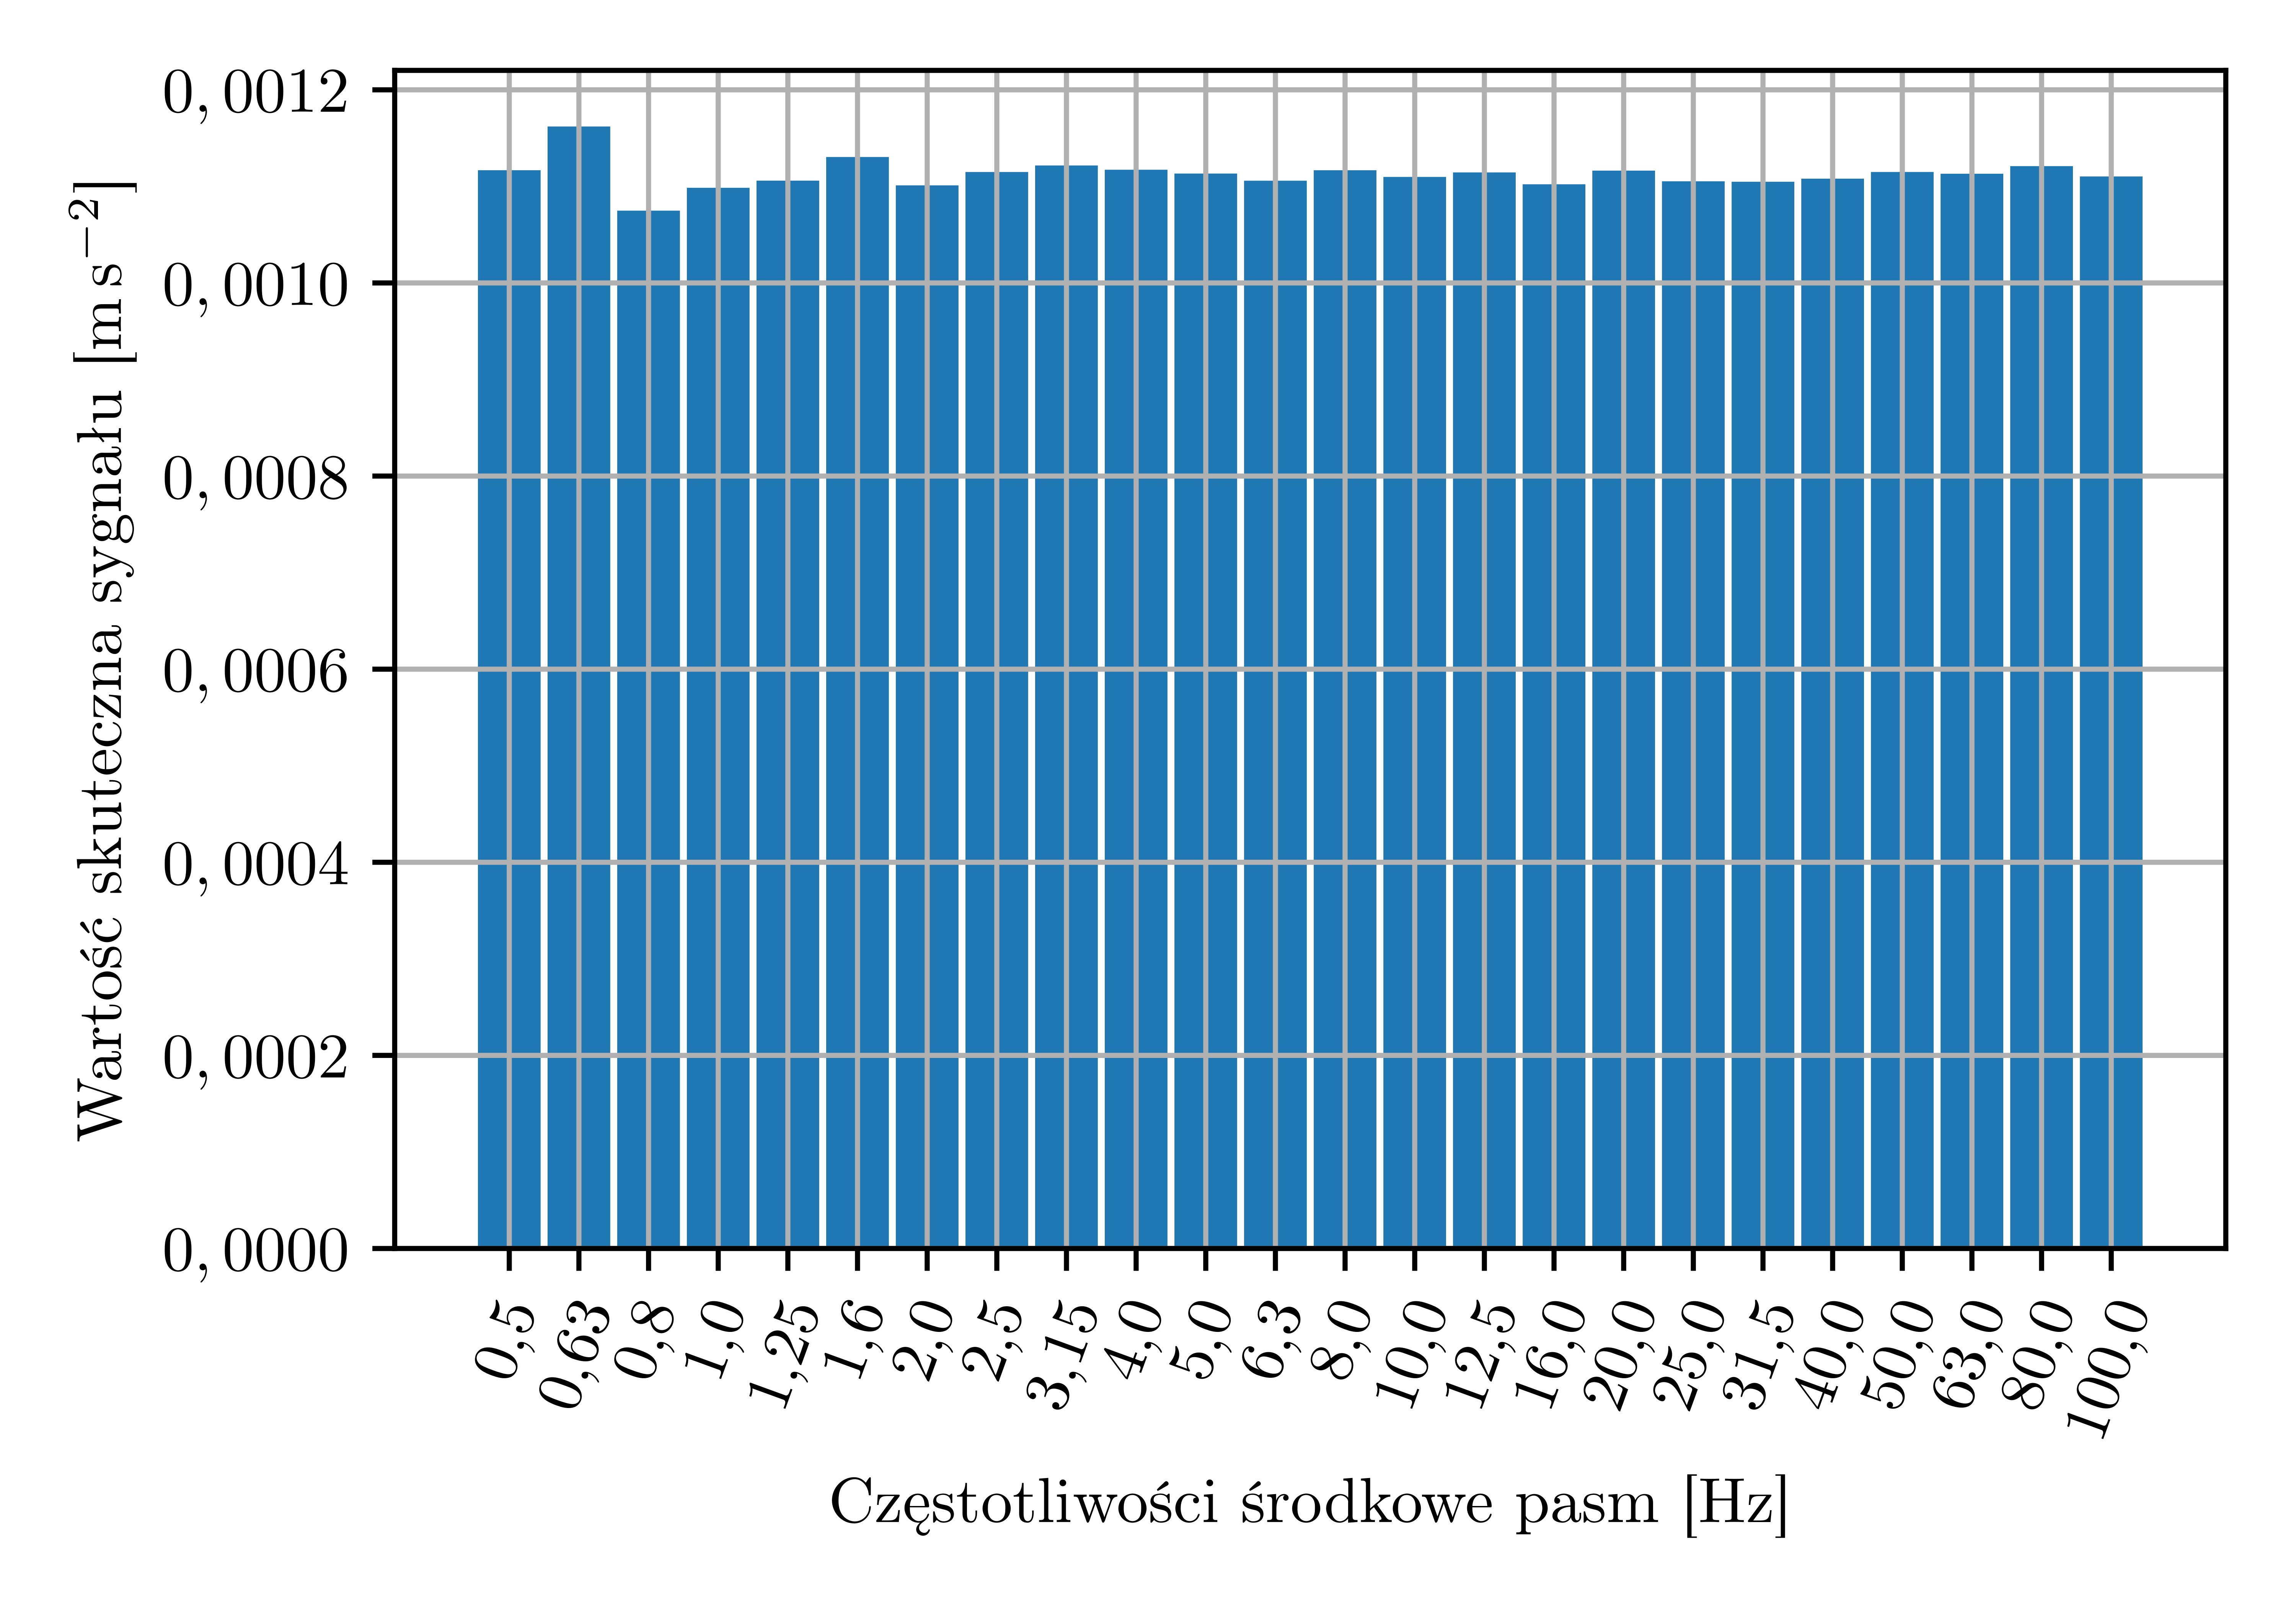
\includegraphics[width=0.8\textwidth]{plots/ghost_x.png}',
    %% Creator: Matplotlib, PGF backend
%%
%% To include the figure in your LaTeX document, write
%%   \input{<filename>.pgf}
%%
%% Make sure the required packages are loaded in your preamble
%%   \usepackage{pgf}
%%
%% Figures using additional raster images can only be included by \input if
%% they are in the same directory as the main LaTeX file. For loading figures
%% from other directories you can use the `import` package
%%   \usepackage{import}
%% and then include the figures with
%%   \import{<path to file>}{<filename>.pgf}
%%
%% Matplotlib used the following preamble
%%   \usepackage[utf8]{inputenc}
%%   \usepackage[T1]{fontenc}
%%   \usepackage{siunitx}
%%
\begingroup%
\makeatletter%
\begin{pgfpicture}%
\pgfpathrectangle{\pgfpointorigin}{\pgfqpoint{5.000000in}{3.500000in}}%
\pgfusepath{use as bounding box, clip}%
\begin{pgfscope}%
\pgfsetbuttcap%
\pgfsetmiterjoin%
\definecolor{currentfill}{rgb}{1.000000,1.000000,1.000000}%
\pgfsetfillcolor{currentfill}%
\pgfsetlinewidth{0.000000pt}%
\definecolor{currentstroke}{rgb}{1.000000,1.000000,1.000000}%
\pgfsetstrokecolor{currentstroke}%
\pgfsetdash{}{0pt}%
\pgfpathmoveto{\pgfqpoint{0.000000in}{0.000000in}}%
\pgfpathlineto{\pgfqpoint{5.000000in}{0.000000in}}%
\pgfpathlineto{\pgfqpoint{5.000000in}{3.500000in}}%
\pgfpathlineto{\pgfqpoint{0.000000in}{3.500000in}}%
\pgfpathclose%
\pgfusepath{fill}%
\end{pgfscope}%
\begin{pgfscope}%
\pgfsetbuttcap%
\pgfsetmiterjoin%
\definecolor{currentfill}{rgb}{1.000000,1.000000,1.000000}%
\pgfsetfillcolor{currentfill}%
\pgfsetlinewidth{0.000000pt}%
\definecolor{currentstroke}{rgb}{0.000000,0.000000,0.000000}%
\pgfsetstrokecolor{currentstroke}%
\pgfsetstrokeopacity{0.000000}%
\pgfsetdash{}{0pt}%
\pgfpathmoveto{\pgfqpoint{0.859499in}{0.780790in}}%
\pgfpathlineto{\pgfqpoint{4.815000in}{0.780790in}}%
\pgfpathlineto{\pgfqpoint{4.815000in}{3.315000in}}%
\pgfpathlineto{\pgfqpoint{0.859499in}{3.315000in}}%
\pgfpathclose%
\pgfusepath{fill}%
\end{pgfscope}%
\begin{pgfscope}%
\pgfpathrectangle{\pgfqpoint{0.859499in}{0.780790in}}{\pgfqpoint{3.955501in}{2.534210in}}%
\pgfusepath{clip}%
\pgfsetbuttcap%
\pgfsetmiterjoin%
\definecolor{currentfill}{rgb}{0.121569,0.466667,0.705882}%
\pgfsetfillcolor{currentfill}%
\pgfsetlinewidth{0.000000pt}%
\definecolor{currentstroke}{rgb}{0.000000,0.000000,0.000000}%
\pgfsetstrokecolor{currentstroke}%
\pgfsetstrokeopacity{0.000000}%
\pgfsetdash{}{0pt}%
\pgfpathmoveto{\pgfqpoint{1.039294in}{0.780790in}}%
\pgfpathlineto{\pgfqpoint{1.174705in}{0.780790in}}%
\pgfpathlineto{\pgfqpoint{1.174705in}{3.100259in}}%
\pgfpathlineto{\pgfqpoint{1.039294in}{3.100259in}}%
\pgfpathclose%
\pgfusepath{fill}%
\end{pgfscope}%
\begin{pgfscope}%
\pgfpathrectangle{\pgfqpoint{0.859499in}{0.780790in}}{\pgfqpoint{3.955501in}{2.534210in}}%
\pgfusepath{clip}%
\pgfsetbuttcap%
\pgfsetmiterjoin%
\definecolor{currentfill}{rgb}{0.121569,0.466667,0.705882}%
\pgfsetfillcolor{currentfill}%
\pgfsetlinewidth{0.000000pt}%
\definecolor{currentstroke}{rgb}{0.000000,0.000000,0.000000}%
\pgfsetstrokecolor{currentstroke}%
\pgfsetstrokeopacity{0.000000}%
\pgfsetdash{}{0pt}%
\pgfpathmoveto{\pgfqpoint{1.189751in}{0.780790in}}%
\pgfpathlineto{\pgfqpoint{1.325162in}{0.780790in}}%
\pgfpathlineto{\pgfqpoint{1.325162in}{3.194323in}}%
\pgfpathlineto{\pgfqpoint{1.189751in}{3.194323in}}%
\pgfpathclose%
\pgfusepath{fill}%
\end{pgfscope}%
\begin{pgfscope}%
\pgfpathrectangle{\pgfqpoint{0.859499in}{0.780790in}}{\pgfqpoint{3.955501in}{2.534210in}}%
\pgfusepath{clip}%
\pgfsetbuttcap%
\pgfsetmiterjoin%
\definecolor{currentfill}{rgb}{0.121569,0.466667,0.705882}%
\pgfsetfillcolor{currentfill}%
\pgfsetlinewidth{0.000000pt}%
\definecolor{currentstroke}{rgb}{0.000000,0.000000,0.000000}%
\pgfsetstrokecolor{currentstroke}%
\pgfsetstrokeopacity{0.000000}%
\pgfsetdash{}{0pt}%
\pgfpathmoveto{\pgfqpoint{1.340207in}{0.780790in}}%
\pgfpathlineto{\pgfqpoint{1.475618in}{0.780790in}}%
\pgfpathlineto{\pgfqpoint{1.475618in}{3.013330in}}%
\pgfpathlineto{\pgfqpoint{1.340207in}{3.013330in}}%
\pgfpathclose%
\pgfusepath{fill}%
\end{pgfscope}%
\begin{pgfscope}%
\pgfpathrectangle{\pgfqpoint{0.859499in}{0.780790in}}{\pgfqpoint{3.955501in}{2.534210in}}%
\pgfusepath{clip}%
\pgfsetbuttcap%
\pgfsetmiterjoin%
\definecolor{currentfill}{rgb}{0.121569,0.466667,0.705882}%
\pgfsetfillcolor{currentfill}%
\pgfsetlinewidth{0.000000pt}%
\definecolor{currentstroke}{rgb}{0.000000,0.000000,0.000000}%
\pgfsetstrokecolor{currentstroke}%
\pgfsetstrokeopacity{0.000000}%
\pgfsetdash{}{0pt}%
\pgfpathmoveto{\pgfqpoint{1.490664in}{0.780790in}}%
\pgfpathlineto{\pgfqpoint{1.626075in}{0.780790in}}%
\pgfpathlineto{\pgfqpoint{1.626075in}{3.062487in}}%
\pgfpathlineto{\pgfqpoint{1.490664in}{3.062487in}}%
\pgfpathclose%
\pgfusepath{fill}%
\end{pgfscope}%
\begin{pgfscope}%
\pgfpathrectangle{\pgfqpoint{0.859499in}{0.780790in}}{\pgfqpoint{3.955501in}{2.534210in}}%
\pgfusepath{clip}%
\pgfsetbuttcap%
\pgfsetmiterjoin%
\definecolor{currentfill}{rgb}{0.121569,0.466667,0.705882}%
\pgfsetfillcolor{currentfill}%
\pgfsetlinewidth{0.000000pt}%
\definecolor{currentstroke}{rgb}{0.000000,0.000000,0.000000}%
\pgfsetstrokecolor{currentstroke}%
\pgfsetstrokeopacity{0.000000}%
\pgfsetdash{}{0pt}%
\pgfpathmoveto{\pgfqpoint{1.641120in}{0.780790in}}%
\pgfpathlineto{\pgfqpoint{1.776531in}{0.780790in}}%
\pgfpathlineto{\pgfqpoint{1.776531in}{3.077827in}}%
\pgfpathlineto{\pgfqpoint{1.641120in}{3.077827in}}%
\pgfpathclose%
\pgfusepath{fill}%
\end{pgfscope}%
\begin{pgfscope}%
\pgfpathrectangle{\pgfqpoint{0.859499in}{0.780790in}}{\pgfqpoint{3.955501in}{2.534210in}}%
\pgfusepath{clip}%
\pgfsetbuttcap%
\pgfsetmiterjoin%
\definecolor{currentfill}{rgb}{0.121569,0.466667,0.705882}%
\pgfsetfillcolor{currentfill}%
\pgfsetlinewidth{0.000000pt}%
\definecolor{currentstroke}{rgb}{0.000000,0.000000,0.000000}%
\pgfsetstrokecolor{currentstroke}%
\pgfsetstrokeopacity{0.000000}%
\pgfsetdash{}{0pt}%
\pgfpathmoveto{\pgfqpoint{1.791577in}{0.780790in}}%
\pgfpathlineto{\pgfqpoint{1.926988in}{0.780790in}}%
\pgfpathlineto{\pgfqpoint{1.926988in}{3.128671in}}%
\pgfpathlineto{\pgfqpoint{1.791577in}{3.128671in}}%
\pgfpathclose%
\pgfusepath{fill}%
\end{pgfscope}%
\begin{pgfscope}%
\pgfpathrectangle{\pgfqpoint{0.859499in}{0.780790in}}{\pgfqpoint{3.955501in}{2.534210in}}%
\pgfusepath{clip}%
\pgfsetbuttcap%
\pgfsetmiterjoin%
\definecolor{currentfill}{rgb}{0.121569,0.466667,0.705882}%
\pgfsetfillcolor{currentfill}%
\pgfsetlinewidth{0.000000pt}%
\definecolor{currentstroke}{rgb}{0.000000,0.000000,0.000000}%
\pgfsetstrokecolor{currentstroke}%
\pgfsetstrokeopacity{0.000000}%
\pgfsetdash{}{0pt}%
\pgfpathmoveto{\pgfqpoint{1.942033in}{0.780790in}}%
\pgfpathlineto{\pgfqpoint{2.077444in}{0.780790in}}%
\pgfpathlineto{\pgfqpoint{2.077444in}{3.067704in}}%
\pgfpathlineto{\pgfqpoint{1.942033in}{3.067704in}}%
\pgfpathclose%
\pgfusepath{fill}%
\end{pgfscope}%
\begin{pgfscope}%
\pgfpathrectangle{\pgfqpoint{0.859499in}{0.780790in}}{\pgfqpoint{3.955501in}{2.534210in}}%
\pgfusepath{clip}%
\pgfsetbuttcap%
\pgfsetmiterjoin%
\definecolor{currentfill}{rgb}{0.121569,0.466667,0.705882}%
\pgfsetfillcolor{currentfill}%
\pgfsetlinewidth{0.000000pt}%
\definecolor{currentstroke}{rgb}{0.000000,0.000000,0.000000}%
\pgfsetstrokecolor{currentstroke}%
\pgfsetstrokeopacity{0.000000}%
\pgfsetdash{}{0pt}%
\pgfpathmoveto{\pgfqpoint{2.092490in}{0.780790in}}%
\pgfpathlineto{\pgfqpoint{2.227901in}{0.780790in}}%
\pgfpathlineto{\pgfqpoint{2.227901in}{3.096442in}}%
\pgfpathlineto{\pgfqpoint{2.092490in}{3.096442in}}%
\pgfpathclose%
\pgfusepath{fill}%
\end{pgfscope}%
\begin{pgfscope}%
\pgfpathrectangle{\pgfqpoint{0.859499in}{0.780790in}}{\pgfqpoint{3.955501in}{2.534210in}}%
\pgfusepath{clip}%
\pgfsetbuttcap%
\pgfsetmiterjoin%
\definecolor{currentfill}{rgb}{0.121569,0.466667,0.705882}%
\pgfsetfillcolor{currentfill}%
\pgfsetlinewidth{0.000000pt}%
\definecolor{currentstroke}{rgb}{0.000000,0.000000,0.000000}%
\pgfsetstrokecolor{currentstroke}%
\pgfsetstrokeopacity{0.000000}%
\pgfsetdash{}{0pt}%
\pgfpathmoveto{\pgfqpoint{2.242946in}{0.780790in}}%
\pgfpathlineto{\pgfqpoint{2.378357in}{0.780790in}}%
\pgfpathlineto{\pgfqpoint{2.378357in}{3.110498in}}%
\pgfpathlineto{\pgfqpoint{2.242946in}{3.110498in}}%
\pgfpathclose%
\pgfusepath{fill}%
\end{pgfscope}%
\begin{pgfscope}%
\pgfpathrectangle{\pgfqpoint{0.859499in}{0.780790in}}{\pgfqpoint{3.955501in}{2.534210in}}%
\pgfusepath{clip}%
\pgfsetbuttcap%
\pgfsetmiterjoin%
\definecolor{currentfill}{rgb}{0.121569,0.466667,0.705882}%
\pgfsetfillcolor{currentfill}%
\pgfsetlinewidth{0.000000pt}%
\definecolor{currentstroke}{rgb}{0.000000,0.000000,0.000000}%
\pgfsetstrokecolor{currentstroke}%
\pgfsetstrokeopacity{0.000000}%
\pgfsetdash{}{0pt}%
\pgfpathmoveto{\pgfqpoint{2.393403in}{0.780790in}}%
\pgfpathlineto{\pgfqpoint{2.528814in}{0.780790in}}%
\pgfpathlineto{\pgfqpoint{2.528814in}{3.101318in}}%
\pgfpathlineto{\pgfqpoint{2.393403in}{3.101318in}}%
\pgfpathclose%
\pgfusepath{fill}%
\end{pgfscope}%
\begin{pgfscope}%
\pgfpathrectangle{\pgfqpoint{0.859499in}{0.780790in}}{\pgfqpoint{3.955501in}{2.534210in}}%
\pgfusepath{clip}%
\pgfsetbuttcap%
\pgfsetmiterjoin%
\definecolor{currentfill}{rgb}{0.121569,0.466667,0.705882}%
\pgfsetfillcolor{currentfill}%
\pgfsetlinewidth{0.000000pt}%
\definecolor{currentstroke}{rgb}{0.000000,0.000000,0.000000}%
\pgfsetstrokecolor{currentstroke}%
\pgfsetstrokeopacity{0.000000}%
\pgfsetdash{}{0pt}%
\pgfpathmoveto{\pgfqpoint{2.543859in}{0.780790in}}%
\pgfpathlineto{\pgfqpoint{2.679270in}{0.780790in}}%
\pgfpathlineto{\pgfqpoint{2.679270in}{3.093089in}}%
\pgfpathlineto{\pgfqpoint{2.543859in}{3.093089in}}%
\pgfpathclose%
\pgfusepath{fill}%
\end{pgfscope}%
\begin{pgfscope}%
\pgfpathrectangle{\pgfqpoint{0.859499in}{0.780790in}}{\pgfqpoint{3.955501in}{2.534210in}}%
\pgfusepath{clip}%
\pgfsetbuttcap%
\pgfsetmiterjoin%
\definecolor{currentfill}{rgb}{0.121569,0.466667,0.705882}%
\pgfsetfillcolor{currentfill}%
\pgfsetlinewidth{0.000000pt}%
\definecolor{currentstroke}{rgb}{0.000000,0.000000,0.000000}%
\pgfsetstrokecolor{currentstroke}%
\pgfsetstrokeopacity{0.000000}%
\pgfsetdash{}{0pt}%
\pgfpathmoveto{\pgfqpoint{2.694316in}{0.780790in}}%
\pgfpathlineto{\pgfqpoint{2.829727in}{0.780790in}}%
\pgfpathlineto{\pgfqpoint{2.829727in}{3.077702in}}%
\pgfpathlineto{\pgfqpoint{2.694316in}{3.077702in}}%
\pgfpathclose%
\pgfusepath{fill}%
\end{pgfscope}%
\begin{pgfscope}%
\pgfpathrectangle{\pgfqpoint{0.859499in}{0.780790in}}{\pgfqpoint{3.955501in}{2.534210in}}%
\pgfusepath{clip}%
\pgfsetbuttcap%
\pgfsetmiterjoin%
\definecolor{currentfill}{rgb}{0.121569,0.466667,0.705882}%
\pgfsetfillcolor{currentfill}%
\pgfsetlinewidth{0.000000pt}%
\definecolor{currentstroke}{rgb}{0.000000,0.000000,0.000000}%
\pgfsetstrokecolor{currentstroke}%
\pgfsetstrokeopacity{0.000000}%
\pgfsetdash{}{0pt}%
\pgfpathmoveto{\pgfqpoint{2.844772in}{0.780790in}}%
\pgfpathlineto{\pgfqpoint{2.980183in}{0.780790in}}%
\pgfpathlineto{\pgfqpoint{2.980183in}{3.100233in}}%
\pgfpathlineto{\pgfqpoint{2.844772in}{3.100233in}}%
\pgfpathclose%
\pgfusepath{fill}%
\end{pgfscope}%
\begin{pgfscope}%
\pgfpathrectangle{\pgfqpoint{0.859499in}{0.780790in}}{\pgfqpoint{3.955501in}{2.534210in}}%
\pgfusepath{clip}%
\pgfsetbuttcap%
\pgfsetmiterjoin%
\definecolor{currentfill}{rgb}{0.121569,0.466667,0.705882}%
\pgfsetfillcolor{currentfill}%
\pgfsetlinewidth{0.000000pt}%
\definecolor{currentstroke}{rgb}{0.000000,0.000000,0.000000}%
\pgfsetstrokecolor{currentstroke}%
\pgfsetstrokeopacity{0.000000}%
\pgfsetdash{}{0pt}%
\pgfpathmoveto{\pgfqpoint{2.995229in}{0.780790in}}%
\pgfpathlineto{\pgfqpoint{3.130640in}{0.780790in}}%
\pgfpathlineto{\pgfqpoint{3.130640in}{3.085830in}}%
\pgfpathlineto{\pgfqpoint{2.995229in}{3.085830in}}%
\pgfpathclose%
\pgfusepath{fill}%
\end{pgfscope}%
\begin{pgfscope}%
\pgfpathrectangle{\pgfqpoint{0.859499in}{0.780790in}}{\pgfqpoint{3.955501in}{2.534210in}}%
\pgfusepath{clip}%
\pgfsetbuttcap%
\pgfsetmiterjoin%
\definecolor{currentfill}{rgb}{0.121569,0.466667,0.705882}%
\pgfsetfillcolor{currentfill}%
\pgfsetlinewidth{0.000000pt}%
\definecolor{currentstroke}{rgb}{0.000000,0.000000,0.000000}%
\pgfsetstrokecolor{currentstroke}%
\pgfsetstrokeopacity{0.000000}%
\pgfsetdash{}{0pt}%
\pgfpathmoveto{\pgfqpoint{3.145685in}{0.780790in}}%
\pgfpathlineto{\pgfqpoint{3.281096in}{0.780790in}}%
\pgfpathlineto{\pgfqpoint{3.281096in}{3.095515in}}%
\pgfpathlineto{\pgfqpoint{3.145685in}{3.095515in}}%
\pgfpathclose%
\pgfusepath{fill}%
\end{pgfscope}%
\begin{pgfscope}%
\pgfpathrectangle{\pgfqpoint{0.859499in}{0.780790in}}{\pgfqpoint{3.955501in}{2.534210in}}%
\pgfusepath{clip}%
\pgfsetbuttcap%
\pgfsetmiterjoin%
\definecolor{currentfill}{rgb}{0.121569,0.466667,0.705882}%
\pgfsetfillcolor{currentfill}%
\pgfsetlinewidth{0.000000pt}%
\definecolor{currentstroke}{rgb}{0.000000,0.000000,0.000000}%
\pgfsetstrokecolor{currentstroke}%
\pgfsetstrokeopacity{0.000000}%
\pgfsetdash{}{0pt}%
\pgfpathmoveto{\pgfqpoint{3.296142in}{0.780790in}}%
\pgfpathlineto{\pgfqpoint{3.431553in}{0.780790in}}%
\pgfpathlineto{\pgfqpoint{3.431553in}{3.070029in}}%
\pgfpathlineto{\pgfqpoint{3.296142in}{3.070029in}}%
\pgfpathclose%
\pgfusepath{fill}%
\end{pgfscope}%
\begin{pgfscope}%
\pgfpathrectangle{\pgfqpoint{0.859499in}{0.780790in}}{\pgfqpoint{3.955501in}{2.534210in}}%
\pgfusepath{clip}%
\pgfsetbuttcap%
\pgfsetmiterjoin%
\definecolor{currentfill}{rgb}{0.121569,0.466667,0.705882}%
\pgfsetfillcolor{currentfill}%
\pgfsetlinewidth{0.000000pt}%
\definecolor{currentstroke}{rgb}{0.000000,0.000000,0.000000}%
\pgfsetstrokecolor{currentstroke}%
\pgfsetstrokeopacity{0.000000}%
\pgfsetdash{}{0pt}%
\pgfpathmoveto{\pgfqpoint{3.446598in}{0.780790in}}%
\pgfpathlineto{\pgfqpoint{3.582009in}{0.780790in}}%
\pgfpathlineto{\pgfqpoint{3.582009in}{3.099406in}}%
\pgfpathlineto{\pgfqpoint{3.446598in}{3.099406in}}%
\pgfpathclose%
\pgfusepath{fill}%
\end{pgfscope}%
\begin{pgfscope}%
\pgfpathrectangle{\pgfqpoint{0.859499in}{0.780790in}}{\pgfqpoint{3.955501in}{2.534210in}}%
\pgfusepath{clip}%
\pgfsetbuttcap%
\pgfsetmiterjoin%
\definecolor{currentfill}{rgb}{0.121569,0.466667,0.705882}%
\pgfsetfillcolor{currentfill}%
\pgfsetlinewidth{0.000000pt}%
\definecolor{currentstroke}{rgb}{0.000000,0.000000,0.000000}%
\pgfsetstrokecolor{currentstroke}%
\pgfsetstrokeopacity{0.000000}%
\pgfsetdash{}{0pt}%
\pgfpathmoveto{\pgfqpoint{3.597055in}{0.780790in}}%
\pgfpathlineto{\pgfqpoint{3.732466in}{0.780790in}}%
\pgfpathlineto{\pgfqpoint{3.732466in}{3.076446in}}%
\pgfpathlineto{\pgfqpoint{3.597055in}{3.076446in}}%
\pgfpathclose%
\pgfusepath{fill}%
\end{pgfscope}%
\begin{pgfscope}%
\pgfpathrectangle{\pgfqpoint{0.859499in}{0.780790in}}{\pgfqpoint{3.955501in}{2.534210in}}%
\pgfusepath{clip}%
\pgfsetbuttcap%
\pgfsetmiterjoin%
\definecolor{currentfill}{rgb}{0.121569,0.466667,0.705882}%
\pgfsetfillcolor{currentfill}%
\pgfsetlinewidth{0.000000pt}%
\definecolor{currentstroke}{rgb}{0.000000,0.000000,0.000000}%
\pgfsetstrokecolor{currentstroke}%
\pgfsetstrokeopacity{0.000000}%
\pgfsetdash{}{0pt}%
\pgfpathmoveto{\pgfqpoint{3.747511in}{0.780790in}}%
\pgfpathlineto{\pgfqpoint{3.882922in}{0.780790in}}%
\pgfpathlineto{\pgfqpoint{3.882922in}{3.075408in}}%
\pgfpathlineto{\pgfqpoint{3.747511in}{3.075408in}}%
\pgfpathclose%
\pgfusepath{fill}%
\end{pgfscope}%
\begin{pgfscope}%
\pgfpathrectangle{\pgfqpoint{0.859499in}{0.780790in}}{\pgfqpoint{3.955501in}{2.534210in}}%
\pgfusepath{clip}%
\pgfsetbuttcap%
\pgfsetmiterjoin%
\definecolor{currentfill}{rgb}{0.121569,0.466667,0.705882}%
\pgfsetfillcolor{currentfill}%
\pgfsetlinewidth{0.000000pt}%
\definecolor{currentstroke}{rgb}{0.000000,0.000000,0.000000}%
\pgfsetstrokecolor{currentstroke}%
\pgfsetstrokeopacity{0.000000}%
\pgfsetdash{}{0pt}%
\pgfpathmoveto{\pgfqpoint{3.897968in}{0.780790in}}%
\pgfpathlineto{\pgfqpoint{4.033379in}{0.780790in}}%
\pgfpathlineto{\pgfqpoint{4.033379in}{3.082073in}}%
\pgfpathlineto{\pgfqpoint{3.897968in}{3.082073in}}%
\pgfpathclose%
\pgfusepath{fill}%
\end{pgfscope}%
\begin{pgfscope}%
\pgfpathrectangle{\pgfqpoint{0.859499in}{0.780790in}}{\pgfqpoint{3.955501in}{2.534210in}}%
\pgfusepath{clip}%
\pgfsetbuttcap%
\pgfsetmiterjoin%
\definecolor{currentfill}{rgb}{0.121569,0.466667,0.705882}%
\pgfsetfillcolor{currentfill}%
\pgfsetlinewidth{0.000000pt}%
\definecolor{currentstroke}{rgb}{0.000000,0.000000,0.000000}%
\pgfsetstrokecolor{currentstroke}%
\pgfsetstrokeopacity{0.000000}%
\pgfsetdash{}{0pt}%
\pgfpathmoveto{\pgfqpoint{4.048424in}{0.780790in}}%
\pgfpathlineto{\pgfqpoint{4.183835in}{0.780790in}}%
\pgfpathlineto{\pgfqpoint{4.183835in}{3.096495in}}%
\pgfpathlineto{\pgfqpoint{4.048424in}{3.096495in}}%
\pgfpathclose%
\pgfusepath{fill}%
\end{pgfscope}%
\begin{pgfscope}%
\pgfpathrectangle{\pgfqpoint{0.859499in}{0.780790in}}{\pgfqpoint{3.955501in}{2.534210in}}%
\pgfusepath{clip}%
\pgfsetbuttcap%
\pgfsetmiterjoin%
\definecolor{currentfill}{rgb}{0.121569,0.466667,0.705882}%
\pgfsetfillcolor{currentfill}%
\pgfsetlinewidth{0.000000pt}%
\definecolor{currentstroke}{rgb}{0.000000,0.000000,0.000000}%
\pgfsetstrokecolor{currentstroke}%
\pgfsetstrokeopacity{0.000000}%
\pgfsetdash{}{0pt}%
\pgfpathmoveto{\pgfqpoint{4.198881in}{0.780790in}}%
\pgfpathlineto{\pgfqpoint{4.334291in}{0.780790in}}%
\pgfpathlineto{\pgfqpoint{4.334291in}{3.092733in}}%
\pgfpathlineto{\pgfqpoint{4.198881in}{3.092733in}}%
\pgfpathclose%
\pgfusepath{fill}%
\end{pgfscope}%
\begin{pgfscope}%
\pgfpathrectangle{\pgfqpoint{0.859499in}{0.780790in}}{\pgfqpoint{3.955501in}{2.534210in}}%
\pgfusepath{clip}%
\pgfsetbuttcap%
\pgfsetmiterjoin%
\definecolor{currentfill}{rgb}{0.121569,0.466667,0.705882}%
\pgfsetfillcolor{currentfill}%
\pgfsetlinewidth{0.000000pt}%
\definecolor{currentstroke}{rgb}{0.000000,0.000000,0.000000}%
\pgfsetstrokecolor{currentstroke}%
\pgfsetstrokeopacity{0.000000}%
\pgfsetdash{}{0pt}%
\pgfpathmoveto{\pgfqpoint{4.349337in}{0.780790in}}%
\pgfpathlineto{\pgfqpoint{4.484748in}{0.780790in}}%
\pgfpathlineto{\pgfqpoint{4.484748in}{3.109060in}}%
\pgfpathlineto{\pgfqpoint{4.349337in}{3.109060in}}%
\pgfpathclose%
\pgfusepath{fill}%
\end{pgfscope}%
\begin{pgfscope}%
\pgfpathrectangle{\pgfqpoint{0.859499in}{0.780790in}}{\pgfqpoint{3.955501in}{2.534210in}}%
\pgfusepath{clip}%
\pgfsetbuttcap%
\pgfsetmiterjoin%
\definecolor{currentfill}{rgb}{0.121569,0.466667,0.705882}%
\pgfsetfillcolor{currentfill}%
\pgfsetlinewidth{0.000000pt}%
\definecolor{currentstroke}{rgb}{0.000000,0.000000,0.000000}%
\pgfsetstrokecolor{currentstroke}%
\pgfsetstrokeopacity{0.000000}%
\pgfsetdash{}{0pt}%
\pgfpathmoveto{\pgfqpoint{4.499794in}{0.780790in}}%
\pgfpathlineto{\pgfqpoint{4.635204in}{0.780790in}}%
\pgfpathlineto{\pgfqpoint{4.635204in}{3.086820in}}%
\pgfpathlineto{\pgfqpoint{4.499794in}{3.086820in}}%
\pgfpathclose%
\pgfusepath{fill}%
\end{pgfscope}%
\begin{pgfscope}%
\pgfpathrectangle{\pgfqpoint{0.859499in}{0.780790in}}{\pgfqpoint{3.955501in}{2.534210in}}%
\pgfusepath{clip}%
\pgfsetrectcap%
\pgfsetroundjoin%
\pgfsetlinewidth{0.803000pt}%
\definecolor{currentstroke}{rgb}{0.690196,0.690196,0.690196}%
\pgfsetstrokecolor{currentstroke}%
\pgfsetdash{}{0pt}%
\pgfpathmoveto{\pgfqpoint{1.107000in}{0.780790in}}%
\pgfpathlineto{\pgfqpoint{1.107000in}{3.315000in}}%
\pgfusepath{stroke}%
\end{pgfscope}%
\begin{pgfscope}%
\pgfsetbuttcap%
\pgfsetroundjoin%
\definecolor{currentfill}{rgb}{0.000000,0.000000,0.000000}%
\pgfsetfillcolor{currentfill}%
\pgfsetlinewidth{0.803000pt}%
\definecolor{currentstroke}{rgb}{0.000000,0.000000,0.000000}%
\pgfsetstrokecolor{currentstroke}%
\pgfsetdash{}{0pt}%
\pgfsys@defobject{currentmarker}{\pgfqpoint{0.000000in}{-0.048611in}}{\pgfqpoint{0.000000in}{0.000000in}}{%
\pgfpathmoveto{\pgfqpoint{0.000000in}{0.000000in}}%
\pgfpathlineto{\pgfqpoint{0.000000in}{-0.048611in}}%
\pgfusepath{stroke,fill}%
}%
\begin{pgfscope}%
\pgfsys@transformshift{1.107000in}{0.780790in}%
\pgfsys@useobject{currentmarker}{}%
\end{pgfscope}%
\end{pgfscope}%
\begin{pgfscope}%
\pgftext[x=1.108916in,y=0.484126in,left,base,rotate=70.000000]{\rmfamily\fontsize{10.000000}{12.000000}\selectfont 0,5}%
\end{pgfscope}%
\begin{pgfscope}%
\pgfpathrectangle{\pgfqpoint{0.859499in}{0.780790in}}{\pgfqpoint{3.955501in}{2.534210in}}%
\pgfusepath{clip}%
\pgfsetrectcap%
\pgfsetroundjoin%
\pgfsetlinewidth{0.803000pt}%
\definecolor{currentstroke}{rgb}{0.690196,0.690196,0.690196}%
\pgfsetstrokecolor{currentstroke}%
\pgfsetdash{}{0pt}%
\pgfpathmoveto{\pgfqpoint{1.257456in}{0.780790in}}%
\pgfpathlineto{\pgfqpoint{1.257456in}{3.315000in}}%
\pgfusepath{stroke}%
\end{pgfscope}%
\begin{pgfscope}%
\pgfsetbuttcap%
\pgfsetroundjoin%
\definecolor{currentfill}{rgb}{0.000000,0.000000,0.000000}%
\pgfsetfillcolor{currentfill}%
\pgfsetlinewidth{0.803000pt}%
\definecolor{currentstroke}{rgb}{0.000000,0.000000,0.000000}%
\pgfsetstrokecolor{currentstroke}%
\pgfsetdash{}{0pt}%
\pgfsys@defobject{currentmarker}{\pgfqpoint{0.000000in}{-0.048611in}}{\pgfqpoint{0.000000in}{0.000000in}}{%
\pgfpathmoveto{\pgfqpoint{0.000000in}{0.000000in}}%
\pgfpathlineto{\pgfqpoint{0.000000in}{-0.048611in}}%
\pgfusepath{stroke,fill}%
}%
\begin{pgfscope}%
\pgfsys@transformshift{1.257456in}{0.780790in}%
\pgfsys@useobject{currentmarker}{}%
\end{pgfscope}%
\end{pgfscope}%
\begin{pgfscope}%
\pgftext[x=1.247500in,y=0.418885in,left,base,rotate=70.000000]{\rmfamily\fontsize{10.000000}{12.000000}\selectfont 0,63}%
\end{pgfscope}%
\begin{pgfscope}%
\pgfpathrectangle{\pgfqpoint{0.859499in}{0.780790in}}{\pgfqpoint{3.955501in}{2.534210in}}%
\pgfusepath{clip}%
\pgfsetrectcap%
\pgfsetroundjoin%
\pgfsetlinewidth{0.803000pt}%
\definecolor{currentstroke}{rgb}{0.690196,0.690196,0.690196}%
\pgfsetstrokecolor{currentstroke}%
\pgfsetdash{}{0pt}%
\pgfpathmoveto{\pgfqpoint{1.407913in}{0.780790in}}%
\pgfpathlineto{\pgfqpoint{1.407913in}{3.315000in}}%
\pgfusepath{stroke}%
\end{pgfscope}%
\begin{pgfscope}%
\pgfsetbuttcap%
\pgfsetroundjoin%
\definecolor{currentfill}{rgb}{0.000000,0.000000,0.000000}%
\pgfsetfillcolor{currentfill}%
\pgfsetlinewidth{0.803000pt}%
\definecolor{currentstroke}{rgb}{0.000000,0.000000,0.000000}%
\pgfsetstrokecolor{currentstroke}%
\pgfsetdash{}{0pt}%
\pgfsys@defobject{currentmarker}{\pgfqpoint{0.000000in}{-0.048611in}}{\pgfqpoint{0.000000in}{0.000000in}}{%
\pgfpathmoveto{\pgfqpoint{0.000000in}{0.000000in}}%
\pgfpathlineto{\pgfqpoint{0.000000in}{-0.048611in}}%
\pgfusepath{stroke,fill}%
}%
\begin{pgfscope}%
\pgfsys@transformshift{1.407913in}{0.780790in}%
\pgfsys@useobject{currentmarker}{}%
\end{pgfscope}%
\end{pgfscope}%
\begin{pgfscope}%
\pgftext[x=1.409829in,y=0.484126in,left,base,rotate=70.000000]{\rmfamily\fontsize{10.000000}{12.000000}\selectfont 0,8}%
\end{pgfscope}%
\begin{pgfscope}%
\pgfpathrectangle{\pgfqpoint{0.859499in}{0.780790in}}{\pgfqpoint{3.955501in}{2.534210in}}%
\pgfusepath{clip}%
\pgfsetrectcap%
\pgfsetroundjoin%
\pgfsetlinewidth{0.803000pt}%
\definecolor{currentstroke}{rgb}{0.690196,0.690196,0.690196}%
\pgfsetstrokecolor{currentstroke}%
\pgfsetdash{}{0pt}%
\pgfpathmoveto{\pgfqpoint{1.558369in}{0.780790in}}%
\pgfpathlineto{\pgfqpoint{1.558369in}{3.315000in}}%
\pgfusepath{stroke}%
\end{pgfscope}%
\begin{pgfscope}%
\pgfsetbuttcap%
\pgfsetroundjoin%
\definecolor{currentfill}{rgb}{0.000000,0.000000,0.000000}%
\pgfsetfillcolor{currentfill}%
\pgfsetlinewidth{0.803000pt}%
\definecolor{currentstroke}{rgb}{0.000000,0.000000,0.000000}%
\pgfsetstrokecolor{currentstroke}%
\pgfsetdash{}{0pt}%
\pgfsys@defobject{currentmarker}{\pgfqpoint{0.000000in}{-0.048611in}}{\pgfqpoint{0.000000in}{0.000000in}}{%
\pgfpathmoveto{\pgfqpoint{0.000000in}{0.000000in}}%
\pgfpathlineto{\pgfqpoint{0.000000in}{-0.048611in}}%
\pgfusepath{stroke,fill}%
}%
\begin{pgfscope}%
\pgfsys@transformshift{1.558369in}{0.780790in}%
\pgfsys@useobject{currentmarker}{}%
\end{pgfscope}%
\end{pgfscope}%
\begin{pgfscope}%
\pgftext[x=1.560285in,y=0.484126in,left,base,rotate=70.000000]{\rmfamily\fontsize{10.000000}{12.000000}\selectfont 1,0}%
\end{pgfscope}%
\begin{pgfscope}%
\pgfpathrectangle{\pgfqpoint{0.859499in}{0.780790in}}{\pgfqpoint{3.955501in}{2.534210in}}%
\pgfusepath{clip}%
\pgfsetrectcap%
\pgfsetroundjoin%
\pgfsetlinewidth{0.803000pt}%
\definecolor{currentstroke}{rgb}{0.690196,0.690196,0.690196}%
\pgfsetstrokecolor{currentstroke}%
\pgfsetdash{}{0pt}%
\pgfpathmoveto{\pgfqpoint{1.708826in}{0.780790in}}%
\pgfpathlineto{\pgfqpoint{1.708826in}{3.315000in}}%
\pgfusepath{stroke}%
\end{pgfscope}%
\begin{pgfscope}%
\pgfsetbuttcap%
\pgfsetroundjoin%
\definecolor{currentfill}{rgb}{0.000000,0.000000,0.000000}%
\pgfsetfillcolor{currentfill}%
\pgfsetlinewidth{0.803000pt}%
\definecolor{currentstroke}{rgb}{0.000000,0.000000,0.000000}%
\pgfsetstrokecolor{currentstroke}%
\pgfsetdash{}{0pt}%
\pgfsys@defobject{currentmarker}{\pgfqpoint{0.000000in}{-0.048611in}}{\pgfqpoint{0.000000in}{0.000000in}}{%
\pgfpathmoveto{\pgfqpoint{0.000000in}{0.000000in}}%
\pgfpathlineto{\pgfqpoint{0.000000in}{-0.048611in}}%
\pgfusepath{stroke,fill}%
}%
\begin{pgfscope}%
\pgfsys@transformshift{1.708826in}{0.780790in}%
\pgfsys@useobject{currentmarker}{}%
\end{pgfscope}%
\end{pgfscope}%
\begin{pgfscope}%
\pgftext[x=1.698869in,y=0.418885in,left,base,rotate=70.000000]{\rmfamily\fontsize{10.000000}{12.000000}\selectfont 1,25}%
\end{pgfscope}%
\begin{pgfscope}%
\pgfpathrectangle{\pgfqpoint{0.859499in}{0.780790in}}{\pgfqpoint{3.955501in}{2.534210in}}%
\pgfusepath{clip}%
\pgfsetrectcap%
\pgfsetroundjoin%
\pgfsetlinewidth{0.803000pt}%
\definecolor{currentstroke}{rgb}{0.690196,0.690196,0.690196}%
\pgfsetstrokecolor{currentstroke}%
\pgfsetdash{}{0pt}%
\pgfpathmoveto{\pgfqpoint{1.859282in}{0.780790in}}%
\pgfpathlineto{\pgfqpoint{1.859282in}{3.315000in}}%
\pgfusepath{stroke}%
\end{pgfscope}%
\begin{pgfscope}%
\pgfsetbuttcap%
\pgfsetroundjoin%
\definecolor{currentfill}{rgb}{0.000000,0.000000,0.000000}%
\pgfsetfillcolor{currentfill}%
\pgfsetlinewidth{0.803000pt}%
\definecolor{currentstroke}{rgb}{0.000000,0.000000,0.000000}%
\pgfsetstrokecolor{currentstroke}%
\pgfsetdash{}{0pt}%
\pgfsys@defobject{currentmarker}{\pgfqpoint{0.000000in}{-0.048611in}}{\pgfqpoint{0.000000in}{0.000000in}}{%
\pgfpathmoveto{\pgfqpoint{0.000000in}{0.000000in}}%
\pgfpathlineto{\pgfqpoint{0.000000in}{-0.048611in}}%
\pgfusepath{stroke,fill}%
}%
\begin{pgfscope}%
\pgfsys@transformshift{1.859282in}{0.780790in}%
\pgfsys@useobject{currentmarker}{}%
\end{pgfscope}%
\end{pgfscope}%
\begin{pgfscope}%
\pgftext[x=1.861198in,y=0.484126in,left,base,rotate=70.000000]{\rmfamily\fontsize{10.000000}{12.000000}\selectfont 1,6}%
\end{pgfscope}%
\begin{pgfscope}%
\pgfpathrectangle{\pgfqpoint{0.859499in}{0.780790in}}{\pgfqpoint{3.955501in}{2.534210in}}%
\pgfusepath{clip}%
\pgfsetrectcap%
\pgfsetroundjoin%
\pgfsetlinewidth{0.803000pt}%
\definecolor{currentstroke}{rgb}{0.690196,0.690196,0.690196}%
\pgfsetstrokecolor{currentstroke}%
\pgfsetdash{}{0pt}%
\pgfpathmoveto{\pgfqpoint{2.009739in}{0.780790in}}%
\pgfpathlineto{\pgfqpoint{2.009739in}{3.315000in}}%
\pgfusepath{stroke}%
\end{pgfscope}%
\begin{pgfscope}%
\pgfsetbuttcap%
\pgfsetroundjoin%
\definecolor{currentfill}{rgb}{0.000000,0.000000,0.000000}%
\pgfsetfillcolor{currentfill}%
\pgfsetlinewidth{0.803000pt}%
\definecolor{currentstroke}{rgb}{0.000000,0.000000,0.000000}%
\pgfsetstrokecolor{currentstroke}%
\pgfsetdash{}{0pt}%
\pgfsys@defobject{currentmarker}{\pgfqpoint{0.000000in}{-0.048611in}}{\pgfqpoint{0.000000in}{0.000000in}}{%
\pgfpathmoveto{\pgfqpoint{0.000000in}{0.000000in}}%
\pgfpathlineto{\pgfqpoint{0.000000in}{-0.048611in}}%
\pgfusepath{stroke,fill}%
}%
\begin{pgfscope}%
\pgfsys@transformshift{2.009739in}{0.780790in}%
\pgfsys@useobject{currentmarker}{}%
\end{pgfscope}%
\end{pgfscope}%
\begin{pgfscope}%
\pgftext[x=2.011655in,y=0.484126in,left,base,rotate=70.000000]{\rmfamily\fontsize{10.000000}{12.000000}\selectfont 2,0}%
\end{pgfscope}%
\begin{pgfscope}%
\pgfpathrectangle{\pgfqpoint{0.859499in}{0.780790in}}{\pgfqpoint{3.955501in}{2.534210in}}%
\pgfusepath{clip}%
\pgfsetrectcap%
\pgfsetroundjoin%
\pgfsetlinewidth{0.803000pt}%
\definecolor{currentstroke}{rgb}{0.690196,0.690196,0.690196}%
\pgfsetstrokecolor{currentstroke}%
\pgfsetdash{}{0pt}%
\pgfpathmoveto{\pgfqpoint{2.160195in}{0.780790in}}%
\pgfpathlineto{\pgfqpoint{2.160195in}{3.315000in}}%
\pgfusepath{stroke}%
\end{pgfscope}%
\begin{pgfscope}%
\pgfsetbuttcap%
\pgfsetroundjoin%
\definecolor{currentfill}{rgb}{0.000000,0.000000,0.000000}%
\pgfsetfillcolor{currentfill}%
\pgfsetlinewidth{0.803000pt}%
\definecolor{currentstroke}{rgb}{0.000000,0.000000,0.000000}%
\pgfsetstrokecolor{currentstroke}%
\pgfsetdash{}{0pt}%
\pgfsys@defobject{currentmarker}{\pgfqpoint{0.000000in}{-0.048611in}}{\pgfqpoint{0.000000in}{0.000000in}}{%
\pgfpathmoveto{\pgfqpoint{0.000000in}{0.000000in}}%
\pgfpathlineto{\pgfqpoint{0.000000in}{-0.048611in}}%
\pgfusepath{stroke,fill}%
}%
\begin{pgfscope}%
\pgfsys@transformshift{2.160195in}{0.780790in}%
\pgfsys@useobject{currentmarker}{}%
\end{pgfscope}%
\end{pgfscope}%
\begin{pgfscope}%
\pgftext[x=2.162111in,y=0.484126in,left,base,rotate=70.000000]{\rmfamily\fontsize{10.000000}{12.000000}\selectfont 2,5}%
\end{pgfscope}%
\begin{pgfscope}%
\pgfpathrectangle{\pgfqpoint{0.859499in}{0.780790in}}{\pgfqpoint{3.955501in}{2.534210in}}%
\pgfusepath{clip}%
\pgfsetrectcap%
\pgfsetroundjoin%
\pgfsetlinewidth{0.803000pt}%
\definecolor{currentstroke}{rgb}{0.690196,0.690196,0.690196}%
\pgfsetstrokecolor{currentstroke}%
\pgfsetdash{}{0pt}%
\pgfpathmoveto{\pgfqpoint{2.310652in}{0.780790in}}%
\pgfpathlineto{\pgfqpoint{2.310652in}{3.315000in}}%
\pgfusepath{stroke}%
\end{pgfscope}%
\begin{pgfscope}%
\pgfsetbuttcap%
\pgfsetroundjoin%
\definecolor{currentfill}{rgb}{0.000000,0.000000,0.000000}%
\pgfsetfillcolor{currentfill}%
\pgfsetlinewidth{0.803000pt}%
\definecolor{currentstroke}{rgb}{0.000000,0.000000,0.000000}%
\pgfsetstrokecolor{currentstroke}%
\pgfsetdash{}{0pt}%
\pgfsys@defobject{currentmarker}{\pgfqpoint{0.000000in}{-0.048611in}}{\pgfqpoint{0.000000in}{0.000000in}}{%
\pgfpathmoveto{\pgfqpoint{0.000000in}{0.000000in}}%
\pgfpathlineto{\pgfqpoint{0.000000in}{-0.048611in}}%
\pgfusepath{stroke,fill}%
}%
\begin{pgfscope}%
\pgfsys@transformshift{2.310652in}{0.780790in}%
\pgfsys@useobject{currentmarker}{}%
\end{pgfscope}%
\end{pgfscope}%
\begin{pgfscope}%
\pgftext[x=2.300695in,y=0.418885in,left,base,rotate=70.000000]{\rmfamily\fontsize{10.000000}{12.000000}\selectfont 3,15}%
\end{pgfscope}%
\begin{pgfscope}%
\pgfpathrectangle{\pgfqpoint{0.859499in}{0.780790in}}{\pgfqpoint{3.955501in}{2.534210in}}%
\pgfusepath{clip}%
\pgfsetrectcap%
\pgfsetroundjoin%
\pgfsetlinewidth{0.803000pt}%
\definecolor{currentstroke}{rgb}{0.690196,0.690196,0.690196}%
\pgfsetstrokecolor{currentstroke}%
\pgfsetdash{}{0pt}%
\pgfpathmoveto{\pgfqpoint{2.461108in}{0.780790in}}%
\pgfpathlineto{\pgfqpoint{2.461108in}{3.315000in}}%
\pgfusepath{stroke}%
\end{pgfscope}%
\begin{pgfscope}%
\pgfsetbuttcap%
\pgfsetroundjoin%
\definecolor{currentfill}{rgb}{0.000000,0.000000,0.000000}%
\pgfsetfillcolor{currentfill}%
\pgfsetlinewidth{0.803000pt}%
\definecolor{currentstroke}{rgb}{0.000000,0.000000,0.000000}%
\pgfsetstrokecolor{currentstroke}%
\pgfsetdash{}{0pt}%
\pgfsys@defobject{currentmarker}{\pgfqpoint{0.000000in}{-0.048611in}}{\pgfqpoint{0.000000in}{0.000000in}}{%
\pgfpathmoveto{\pgfqpoint{0.000000in}{0.000000in}}%
\pgfpathlineto{\pgfqpoint{0.000000in}{-0.048611in}}%
\pgfusepath{stroke,fill}%
}%
\begin{pgfscope}%
\pgfsys@transformshift{2.461108in}{0.780790in}%
\pgfsys@useobject{currentmarker}{}%
\end{pgfscope}%
\end{pgfscope}%
\begin{pgfscope}%
\pgftext[x=2.463024in,y=0.484126in,left,base,rotate=70.000000]{\rmfamily\fontsize{10.000000}{12.000000}\selectfont 4,0}%
\end{pgfscope}%
\begin{pgfscope}%
\pgfpathrectangle{\pgfqpoint{0.859499in}{0.780790in}}{\pgfqpoint{3.955501in}{2.534210in}}%
\pgfusepath{clip}%
\pgfsetrectcap%
\pgfsetroundjoin%
\pgfsetlinewidth{0.803000pt}%
\definecolor{currentstroke}{rgb}{0.690196,0.690196,0.690196}%
\pgfsetstrokecolor{currentstroke}%
\pgfsetdash{}{0pt}%
\pgfpathmoveto{\pgfqpoint{2.611565in}{0.780790in}}%
\pgfpathlineto{\pgfqpoint{2.611565in}{3.315000in}}%
\pgfusepath{stroke}%
\end{pgfscope}%
\begin{pgfscope}%
\pgfsetbuttcap%
\pgfsetroundjoin%
\definecolor{currentfill}{rgb}{0.000000,0.000000,0.000000}%
\pgfsetfillcolor{currentfill}%
\pgfsetlinewidth{0.803000pt}%
\definecolor{currentstroke}{rgb}{0.000000,0.000000,0.000000}%
\pgfsetstrokecolor{currentstroke}%
\pgfsetdash{}{0pt}%
\pgfsys@defobject{currentmarker}{\pgfqpoint{0.000000in}{-0.048611in}}{\pgfqpoint{0.000000in}{0.000000in}}{%
\pgfpathmoveto{\pgfqpoint{0.000000in}{0.000000in}}%
\pgfpathlineto{\pgfqpoint{0.000000in}{-0.048611in}}%
\pgfusepath{stroke,fill}%
}%
\begin{pgfscope}%
\pgfsys@transformshift{2.611565in}{0.780790in}%
\pgfsys@useobject{currentmarker}{}%
\end{pgfscope}%
\end{pgfscope}%
\begin{pgfscope}%
\pgftext[x=2.613481in,y=0.484126in,left,base,rotate=70.000000]{\rmfamily\fontsize{10.000000}{12.000000}\selectfont 5,0}%
\end{pgfscope}%
\begin{pgfscope}%
\pgfpathrectangle{\pgfqpoint{0.859499in}{0.780790in}}{\pgfqpoint{3.955501in}{2.534210in}}%
\pgfusepath{clip}%
\pgfsetrectcap%
\pgfsetroundjoin%
\pgfsetlinewidth{0.803000pt}%
\definecolor{currentstroke}{rgb}{0.690196,0.690196,0.690196}%
\pgfsetstrokecolor{currentstroke}%
\pgfsetdash{}{0pt}%
\pgfpathmoveto{\pgfqpoint{2.762021in}{0.780790in}}%
\pgfpathlineto{\pgfqpoint{2.762021in}{3.315000in}}%
\pgfusepath{stroke}%
\end{pgfscope}%
\begin{pgfscope}%
\pgfsetbuttcap%
\pgfsetroundjoin%
\definecolor{currentfill}{rgb}{0.000000,0.000000,0.000000}%
\pgfsetfillcolor{currentfill}%
\pgfsetlinewidth{0.803000pt}%
\definecolor{currentstroke}{rgb}{0.000000,0.000000,0.000000}%
\pgfsetstrokecolor{currentstroke}%
\pgfsetdash{}{0pt}%
\pgfsys@defobject{currentmarker}{\pgfqpoint{0.000000in}{-0.048611in}}{\pgfqpoint{0.000000in}{0.000000in}}{%
\pgfpathmoveto{\pgfqpoint{0.000000in}{0.000000in}}%
\pgfpathlineto{\pgfqpoint{0.000000in}{-0.048611in}}%
\pgfusepath{stroke,fill}%
}%
\begin{pgfscope}%
\pgfsys@transformshift{2.762021in}{0.780790in}%
\pgfsys@useobject{currentmarker}{}%
\end{pgfscope}%
\end{pgfscope}%
\begin{pgfscope}%
\pgftext[x=2.763937in,y=0.484126in,left,base,rotate=70.000000]{\rmfamily\fontsize{10.000000}{12.000000}\selectfont 6,3}%
\end{pgfscope}%
\begin{pgfscope}%
\pgfpathrectangle{\pgfqpoint{0.859499in}{0.780790in}}{\pgfqpoint{3.955501in}{2.534210in}}%
\pgfusepath{clip}%
\pgfsetrectcap%
\pgfsetroundjoin%
\pgfsetlinewidth{0.803000pt}%
\definecolor{currentstroke}{rgb}{0.690196,0.690196,0.690196}%
\pgfsetstrokecolor{currentstroke}%
\pgfsetdash{}{0pt}%
\pgfpathmoveto{\pgfqpoint{2.912478in}{0.780790in}}%
\pgfpathlineto{\pgfqpoint{2.912478in}{3.315000in}}%
\pgfusepath{stroke}%
\end{pgfscope}%
\begin{pgfscope}%
\pgfsetbuttcap%
\pgfsetroundjoin%
\definecolor{currentfill}{rgb}{0.000000,0.000000,0.000000}%
\pgfsetfillcolor{currentfill}%
\pgfsetlinewidth{0.803000pt}%
\definecolor{currentstroke}{rgb}{0.000000,0.000000,0.000000}%
\pgfsetstrokecolor{currentstroke}%
\pgfsetdash{}{0pt}%
\pgfsys@defobject{currentmarker}{\pgfqpoint{0.000000in}{-0.048611in}}{\pgfqpoint{0.000000in}{0.000000in}}{%
\pgfpathmoveto{\pgfqpoint{0.000000in}{0.000000in}}%
\pgfpathlineto{\pgfqpoint{0.000000in}{-0.048611in}}%
\pgfusepath{stroke,fill}%
}%
\begin{pgfscope}%
\pgfsys@transformshift{2.912478in}{0.780790in}%
\pgfsys@useobject{currentmarker}{}%
\end{pgfscope}%
\end{pgfscope}%
\begin{pgfscope}%
\pgftext[x=2.914394in,y=0.484126in,left,base,rotate=70.000000]{\rmfamily\fontsize{10.000000}{12.000000}\selectfont 8,0}%
\end{pgfscope}%
\begin{pgfscope}%
\pgfpathrectangle{\pgfqpoint{0.859499in}{0.780790in}}{\pgfqpoint{3.955501in}{2.534210in}}%
\pgfusepath{clip}%
\pgfsetrectcap%
\pgfsetroundjoin%
\pgfsetlinewidth{0.803000pt}%
\definecolor{currentstroke}{rgb}{0.690196,0.690196,0.690196}%
\pgfsetstrokecolor{currentstroke}%
\pgfsetdash{}{0pt}%
\pgfpathmoveto{\pgfqpoint{3.062934in}{0.780790in}}%
\pgfpathlineto{\pgfqpoint{3.062934in}{3.315000in}}%
\pgfusepath{stroke}%
\end{pgfscope}%
\begin{pgfscope}%
\pgfsetbuttcap%
\pgfsetroundjoin%
\definecolor{currentfill}{rgb}{0.000000,0.000000,0.000000}%
\pgfsetfillcolor{currentfill}%
\pgfsetlinewidth{0.803000pt}%
\definecolor{currentstroke}{rgb}{0.000000,0.000000,0.000000}%
\pgfsetstrokecolor{currentstroke}%
\pgfsetdash{}{0pt}%
\pgfsys@defobject{currentmarker}{\pgfqpoint{0.000000in}{-0.048611in}}{\pgfqpoint{0.000000in}{0.000000in}}{%
\pgfpathmoveto{\pgfqpoint{0.000000in}{0.000000in}}%
\pgfpathlineto{\pgfqpoint{0.000000in}{-0.048611in}}%
\pgfusepath{stroke,fill}%
}%
\begin{pgfscope}%
\pgfsys@transformshift{3.062934in}{0.780790in}%
\pgfsys@useobject{currentmarker}{}%
\end{pgfscope}%
\end{pgfscope}%
\begin{pgfscope}%
\pgftext[x=3.052977in,y=0.418885in,left,base,rotate=70.000000]{\rmfamily\fontsize{10.000000}{12.000000}\selectfont 10,0}%
\end{pgfscope}%
\begin{pgfscope}%
\pgfpathrectangle{\pgfqpoint{0.859499in}{0.780790in}}{\pgfqpoint{3.955501in}{2.534210in}}%
\pgfusepath{clip}%
\pgfsetrectcap%
\pgfsetroundjoin%
\pgfsetlinewidth{0.803000pt}%
\definecolor{currentstroke}{rgb}{0.690196,0.690196,0.690196}%
\pgfsetstrokecolor{currentstroke}%
\pgfsetdash{}{0pt}%
\pgfpathmoveto{\pgfqpoint{3.213391in}{0.780790in}}%
\pgfpathlineto{\pgfqpoint{3.213391in}{3.315000in}}%
\pgfusepath{stroke}%
\end{pgfscope}%
\begin{pgfscope}%
\pgfsetbuttcap%
\pgfsetroundjoin%
\definecolor{currentfill}{rgb}{0.000000,0.000000,0.000000}%
\pgfsetfillcolor{currentfill}%
\pgfsetlinewidth{0.803000pt}%
\definecolor{currentstroke}{rgb}{0.000000,0.000000,0.000000}%
\pgfsetstrokecolor{currentstroke}%
\pgfsetdash{}{0pt}%
\pgfsys@defobject{currentmarker}{\pgfqpoint{0.000000in}{-0.048611in}}{\pgfqpoint{0.000000in}{0.000000in}}{%
\pgfpathmoveto{\pgfqpoint{0.000000in}{0.000000in}}%
\pgfpathlineto{\pgfqpoint{0.000000in}{-0.048611in}}%
\pgfusepath{stroke,fill}%
}%
\begin{pgfscope}%
\pgfsys@transformshift{3.213391in}{0.780790in}%
\pgfsys@useobject{currentmarker}{}%
\end{pgfscope}%
\end{pgfscope}%
\begin{pgfscope}%
\pgftext[x=3.203434in,y=0.418885in,left,base,rotate=70.000000]{\rmfamily\fontsize{10.000000}{12.000000}\selectfont 12,5}%
\end{pgfscope}%
\begin{pgfscope}%
\pgfpathrectangle{\pgfqpoint{0.859499in}{0.780790in}}{\pgfqpoint{3.955501in}{2.534210in}}%
\pgfusepath{clip}%
\pgfsetrectcap%
\pgfsetroundjoin%
\pgfsetlinewidth{0.803000pt}%
\definecolor{currentstroke}{rgb}{0.690196,0.690196,0.690196}%
\pgfsetstrokecolor{currentstroke}%
\pgfsetdash{}{0pt}%
\pgfpathmoveto{\pgfqpoint{3.363847in}{0.780790in}}%
\pgfpathlineto{\pgfqpoint{3.363847in}{3.315000in}}%
\pgfusepath{stroke}%
\end{pgfscope}%
\begin{pgfscope}%
\pgfsetbuttcap%
\pgfsetroundjoin%
\definecolor{currentfill}{rgb}{0.000000,0.000000,0.000000}%
\pgfsetfillcolor{currentfill}%
\pgfsetlinewidth{0.803000pt}%
\definecolor{currentstroke}{rgb}{0.000000,0.000000,0.000000}%
\pgfsetstrokecolor{currentstroke}%
\pgfsetdash{}{0pt}%
\pgfsys@defobject{currentmarker}{\pgfqpoint{0.000000in}{-0.048611in}}{\pgfqpoint{0.000000in}{0.000000in}}{%
\pgfpathmoveto{\pgfqpoint{0.000000in}{0.000000in}}%
\pgfpathlineto{\pgfqpoint{0.000000in}{-0.048611in}}%
\pgfusepath{stroke,fill}%
}%
\begin{pgfscope}%
\pgfsys@transformshift{3.363847in}{0.780790in}%
\pgfsys@useobject{currentmarker}{}%
\end{pgfscope}%
\end{pgfscope}%
\begin{pgfscope}%
\pgftext[x=3.353890in,y=0.418885in,left,base,rotate=70.000000]{\rmfamily\fontsize{10.000000}{12.000000}\selectfont 16,0}%
\end{pgfscope}%
\begin{pgfscope}%
\pgfpathrectangle{\pgfqpoint{0.859499in}{0.780790in}}{\pgfqpoint{3.955501in}{2.534210in}}%
\pgfusepath{clip}%
\pgfsetrectcap%
\pgfsetroundjoin%
\pgfsetlinewidth{0.803000pt}%
\definecolor{currentstroke}{rgb}{0.690196,0.690196,0.690196}%
\pgfsetstrokecolor{currentstroke}%
\pgfsetdash{}{0pt}%
\pgfpathmoveto{\pgfqpoint{3.514304in}{0.780790in}}%
\pgfpathlineto{\pgfqpoint{3.514304in}{3.315000in}}%
\pgfusepath{stroke}%
\end{pgfscope}%
\begin{pgfscope}%
\pgfsetbuttcap%
\pgfsetroundjoin%
\definecolor{currentfill}{rgb}{0.000000,0.000000,0.000000}%
\pgfsetfillcolor{currentfill}%
\pgfsetlinewidth{0.803000pt}%
\definecolor{currentstroke}{rgb}{0.000000,0.000000,0.000000}%
\pgfsetstrokecolor{currentstroke}%
\pgfsetdash{}{0pt}%
\pgfsys@defobject{currentmarker}{\pgfqpoint{0.000000in}{-0.048611in}}{\pgfqpoint{0.000000in}{0.000000in}}{%
\pgfpathmoveto{\pgfqpoint{0.000000in}{0.000000in}}%
\pgfpathlineto{\pgfqpoint{0.000000in}{-0.048611in}}%
\pgfusepath{stroke,fill}%
}%
\begin{pgfscope}%
\pgfsys@transformshift{3.514304in}{0.780790in}%
\pgfsys@useobject{currentmarker}{}%
\end{pgfscope}%
\end{pgfscope}%
\begin{pgfscope}%
\pgftext[x=3.504347in,y=0.418885in,left,base,rotate=70.000000]{\rmfamily\fontsize{10.000000}{12.000000}\selectfont 20,0}%
\end{pgfscope}%
\begin{pgfscope}%
\pgfpathrectangle{\pgfqpoint{0.859499in}{0.780790in}}{\pgfqpoint{3.955501in}{2.534210in}}%
\pgfusepath{clip}%
\pgfsetrectcap%
\pgfsetroundjoin%
\pgfsetlinewidth{0.803000pt}%
\definecolor{currentstroke}{rgb}{0.690196,0.690196,0.690196}%
\pgfsetstrokecolor{currentstroke}%
\pgfsetdash{}{0pt}%
\pgfpathmoveto{\pgfqpoint{3.664760in}{0.780790in}}%
\pgfpathlineto{\pgfqpoint{3.664760in}{3.315000in}}%
\pgfusepath{stroke}%
\end{pgfscope}%
\begin{pgfscope}%
\pgfsetbuttcap%
\pgfsetroundjoin%
\definecolor{currentfill}{rgb}{0.000000,0.000000,0.000000}%
\pgfsetfillcolor{currentfill}%
\pgfsetlinewidth{0.803000pt}%
\definecolor{currentstroke}{rgb}{0.000000,0.000000,0.000000}%
\pgfsetstrokecolor{currentstroke}%
\pgfsetdash{}{0pt}%
\pgfsys@defobject{currentmarker}{\pgfqpoint{0.000000in}{-0.048611in}}{\pgfqpoint{0.000000in}{0.000000in}}{%
\pgfpathmoveto{\pgfqpoint{0.000000in}{0.000000in}}%
\pgfpathlineto{\pgfqpoint{0.000000in}{-0.048611in}}%
\pgfusepath{stroke,fill}%
}%
\begin{pgfscope}%
\pgfsys@transformshift{3.664760in}{0.780790in}%
\pgfsys@useobject{currentmarker}{}%
\end{pgfscope}%
\end{pgfscope}%
\begin{pgfscope}%
\pgftext[x=3.654803in,y=0.418885in,left,base,rotate=70.000000]{\rmfamily\fontsize{10.000000}{12.000000}\selectfont 25,0}%
\end{pgfscope}%
\begin{pgfscope}%
\pgfpathrectangle{\pgfqpoint{0.859499in}{0.780790in}}{\pgfqpoint{3.955501in}{2.534210in}}%
\pgfusepath{clip}%
\pgfsetrectcap%
\pgfsetroundjoin%
\pgfsetlinewidth{0.803000pt}%
\definecolor{currentstroke}{rgb}{0.690196,0.690196,0.690196}%
\pgfsetstrokecolor{currentstroke}%
\pgfsetdash{}{0pt}%
\pgfpathmoveto{\pgfqpoint{3.815217in}{0.780790in}}%
\pgfpathlineto{\pgfqpoint{3.815217in}{3.315000in}}%
\pgfusepath{stroke}%
\end{pgfscope}%
\begin{pgfscope}%
\pgfsetbuttcap%
\pgfsetroundjoin%
\definecolor{currentfill}{rgb}{0.000000,0.000000,0.000000}%
\pgfsetfillcolor{currentfill}%
\pgfsetlinewidth{0.803000pt}%
\definecolor{currentstroke}{rgb}{0.000000,0.000000,0.000000}%
\pgfsetstrokecolor{currentstroke}%
\pgfsetdash{}{0pt}%
\pgfsys@defobject{currentmarker}{\pgfqpoint{0.000000in}{-0.048611in}}{\pgfqpoint{0.000000in}{0.000000in}}{%
\pgfpathmoveto{\pgfqpoint{0.000000in}{0.000000in}}%
\pgfpathlineto{\pgfqpoint{0.000000in}{-0.048611in}}%
\pgfusepath{stroke,fill}%
}%
\begin{pgfscope}%
\pgfsys@transformshift{3.815217in}{0.780790in}%
\pgfsys@useobject{currentmarker}{}%
\end{pgfscope}%
\end{pgfscope}%
\begin{pgfscope}%
\pgftext[x=3.805260in,y=0.418885in,left,base,rotate=70.000000]{\rmfamily\fontsize{10.000000}{12.000000}\selectfont 31,5}%
\end{pgfscope}%
\begin{pgfscope}%
\pgfpathrectangle{\pgfqpoint{0.859499in}{0.780790in}}{\pgfqpoint{3.955501in}{2.534210in}}%
\pgfusepath{clip}%
\pgfsetrectcap%
\pgfsetroundjoin%
\pgfsetlinewidth{0.803000pt}%
\definecolor{currentstroke}{rgb}{0.690196,0.690196,0.690196}%
\pgfsetstrokecolor{currentstroke}%
\pgfsetdash{}{0pt}%
\pgfpathmoveto{\pgfqpoint{3.965673in}{0.780790in}}%
\pgfpathlineto{\pgfqpoint{3.965673in}{3.315000in}}%
\pgfusepath{stroke}%
\end{pgfscope}%
\begin{pgfscope}%
\pgfsetbuttcap%
\pgfsetroundjoin%
\definecolor{currentfill}{rgb}{0.000000,0.000000,0.000000}%
\pgfsetfillcolor{currentfill}%
\pgfsetlinewidth{0.803000pt}%
\definecolor{currentstroke}{rgb}{0.000000,0.000000,0.000000}%
\pgfsetstrokecolor{currentstroke}%
\pgfsetdash{}{0pt}%
\pgfsys@defobject{currentmarker}{\pgfqpoint{0.000000in}{-0.048611in}}{\pgfqpoint{0.000000in}{0.000000in}}{%
\pgfpathmoveto{\pgfqpoint{0.000000in}{0.000000in}}%
\pgfpathlineto{\pgfqpoint{0.000000in}{-0.048611in}}%
\pgfusepath{stroke,fill}%
}%
\begin{pgfscope}%
\pgfsys@transformshift{3.965673in}{0.780790in}%
\pgfsys@useobject{currentmarker}{}%
\end{pgfscope}%
\end{pgfscope}%
\begin{pgfscope}%
\pgftext[x=3.955716in,y=0.418885in,left,base,rotate=70.000000]{\rmfamily\fontsize{10.000000}{12.000000}\selectfont 40,0}%
\end{pgfscope}%
\begin{pgfscope}%
\pgfpathrectangle{\pgfqpoint{0.859499in}{0.780790in}}{\pgfqpoint{3.955501in}{2.534210in}}%
\pgfusepath{clip}%
\pgfsetrectcap%
\pgfsetroundjoin%
\pgfsetlinewidth{0.803000pt}%
\definecolor{currentstroke}{rgb}{0.690196,0.690196,0.690196}%
\pgfsetstrokecolor{currentstroke}%
\pgfsetdash{}{0pt}%
\pgfpathmoveto{\pgfqpoint{4.116130in}{0.780790in}}%
\pgfpathlineto{\pgfqpoint{4.116130in}{3.315000in}}%
\pgfusepath{stroke}%
\end{pgfscope}%
\begin{pgfscope}%
\pgfsetbuttcap%
\pgfsetroundjoin%
\definecolor{currentfill}{rgb}{0.000000,0.000000,0.000000}%
\pgfsetfillcolor{currentfill}%
\pgfsetlinewidth{0.803000pt}%
\definecolor{currentstroke}{rgb}{0.000000,0.000000,0.000000}%
\pgfsetstrokecolor{currentstroke}%
\pgfsetdash{}{0pt}%
\pgfsys@defobject{currentmarker}{\pgfqpoint{0.000000in}{-0.048611in}}{\pgfqpoint{0.000000in}{0.000000in}}{%
\pgfpathmoveto{\pgfqpoint{0.000000in}{0.000000in}}%
\pgfpathlineto{\pgfqpoint{0.000000in}{-0.048611in}}%
\pgfusepath{stroke,fill}%
}%
\begin{pgfscope}%
\pgfsys@transformshift{4.116130in}{0.780790in}%
\pgfsys@useobject{currentmarker}{}%
\end{pgfscope}%
\end{pgfscope}%
\begin{pgfscope}%
\pgftext[x=4.106173in,y=0.418885in,left,base,rotate=70.000000]{\rmfamily\fontsize{10.000000}{12.000000}\selectfont 50,0}%
\end{pgfscope}%
\begin{pgfscope}%
\pgfpathrectangle{\pgfqpoint{0.859499in}{0.780790in}}{\pgfqpoint{3.955501in}{2.534210in}}%
\pgfusepath{clip}%
\pgfsetrectcap%
\pgfsetroundjoin%
\pgfsetlinewidth{0.803000pt}%
\definecolor{currentstroke}{rgb}{0.690196,0.690196,0.690196}%
\pgfsetstrokecolor{currentstroke}%
\pgfsetdash{}{0pt}%
\pgfpathmoveto{\pgfqpoint{4.266586in}{0.780790in}}%
\pgfpathlineto{\pgfqpoint{4.266586in}{3.315000in}}%
\pgfusepath{stroke}%
\end{pgfscope}%
\begin{pgfscope}%
\pgfsetbuttcap%
\pgfsetroundjoin%
\definecolor{currentfill}{rgb}{0.000000,0.000000,0.000000}%
\pgfsetfillcolor{currentfill}%
\pgfsetlinewidth{0.803000pt}%
\definecolor{currentstroke}{rgb}{0.000000,0.000000,0.000000}%
\pgfsetstrokecolor{currentstroke}%
\pgfsetdash{}{0pt}%
\pgfsys@defobject{currentmarker}{\pgfqpoint{0.000000in}{-0.048611in}}{\pgfqpoint{0.000000in}{0.000000in}}{%
\pgfpathmoveto{\pgfqpoint{0.000000in}{0.000000in}}%
\pgfpathlineto{\pgfqpoint{0.000000in}{-0.048611in}}%
\pgfusepath{stroke,fill}%
}%
\begin{pgfscope}%
\pgfsys@transformshift{4.266586in}{0.780790in}%
\pgfsys@useobject{currentmarker}{}%
\end{pgfscope}%
\end{pgfscope}%
\begin{pgfscope}%
\pgftext[x=4.256629in,y=0.418885in,left,base,rotate=70.000000]{\rmfamily\fontsize{10.000000}{12.000000}\selectfont 63,0}%
\end{pgfscope}%
\begin{pgfscope}%
\pgfpathrectangle{\pgfqpoint{0.859499in}{0.780790in}}{\pgfqpoint{3.955501in}{2.534210in}}%
\pgfusepath{clip}%
\pgfsetrectcap%
\pgfsetroundjoin%
\pgfsetlinewidth{0.803000pt}%
\definecolor{currentstroke}{rgb}{0.690196,0.690196,0.690196}%
\pgfsetstrokecolor{currentstroke}%
\pgfsetdash{}{0pt}%
\pgfpathmoveto{\pgfqpoint{4.417043in}{0.780790in}}%
\pgfpathlineto{\pgfqpoint{4.417043in}{3.315000in}}%
\pgfusepath{stroke}%
\end{pgfscope}%
\begin{pgfscope}%
\pgfsetbuttcap%
\pgfsetroundjoin%
\definecolor{currentfill}{rgb}{0.000000,0.000000,0.000000}%
\pgfsetfillcolor{currentfill}%
\pgfsetlinewidth{0.803000pt}%
\definecolor{currentstroke}{rgb}{0.000000,0.000000,0.000000}%
\pgfsetstrokecolor{currentstroke}%
\pgfsetdash{}{0pt}%
\pgfsys@defobject{currentmarker}{\pgfqpoint{0.000000in}{-0.048611in}}{\pgfqpoint{0.000000in}{0.000000in}}{%
\pgfpathmoveto{\pgfqpoint{0.000000in}{0.000000in}}%
\pgfpathlineto{\pgfqpoint{0.000000in}{-0.048611in}}%
\pgfusepath{stroke,fill}%
}%
\begin{pgfscope}%
\pgfsys@transformshift{4.417043in}{0.780790in}%
\pgfsys@useobject{currentmarker}{}%
\end{pgfscope}%
\end{pgfscope}%
\begin{pgfscope}%
\pgftext[x=4.407086in,y=0.418885in,left,base,rotate=70.000000]{\rmfamily\fontsize{10.000000}{12.000000}\selectfont 80,0}%
\end{pgfscope}%
\begin{pgfscope}%
\pgfpathrectangle{\pgfqpoint{0.859499in}{0.780790in}}{\pgfqpoint{3.955501in}{2.534210in}}%
\pgfusepath{clip}%
\pgfsetrectcap%
\pgfsetroundjoin%
\pgfsetlinewidth{0.803000pt}%
\definecolor{currentstroke}{rgb}{0.690196,0.690196,0.690196}%
\pgfsetstrokecolor{currentstroke}%
\pgfsetdash{}{0pt}%
\pgfpathmoveto{\pgfqpoint{4.567499in}{0.780790in}}%
\pgfpathlineto{\pgfqpoint{4.567499in}{3.315000in}}%
\pgfusepath{stroke}%
\end{pgfscope}%
\begin{pgfscope}%
\pgfsetbuttcap%
\pgfsetroundjoin%
\definecolor{currentfill}{rgb}{0.000000,0.000000,0.000000}%
\pgfsetfillcolor{currentfill}%
\pgfsetlinewidth{0.803000pt}%
\definecolor{currentstroke}{rgb}{0.000000,0.000000,0.000000}%
\pgfsetstrokecolor{currentstroke}%
\pgfsetdash{}{0pt}%
\pgfsys@defobject{currentmarker}{\pgfqpoint{0.000000in}{-0.048611in}}{\pgfqpoint{0.000000in}{0.000000in}}{%
\pgfpathmoveto{\pgfqpoint{0.000000in}{0.000000in}}%
\pgfpathlineto{\pgfqpoint{0.000000in}{-0.048611in}}%
\pgfusepath{stroke,fill}%
}%
\begin{pgfscope}%
\pgfsys@transformshift{4.567499in}{0.780790in}%
\pgfsys@useobject{currentmarker}{}%
\end{pgfscope}%
\end{pgfscope}%
\begin{pgfscope}%
\pgftext[x=4.545670in,y=0.353645in,left,base,rotate=70.000000]{\rmfamily\fontsize{10.000000}{12.000000}\selectfont 100,0}%
\end{pgfscope}%
\begin{pgfscope}%
\pgftext[x=2.837249in,y=0.288855in,,top]{\rmfamily\fontsize{10.000000}{12.000000}\selectfont Częstotliwości środkowe pasm [\si{\hertz}]}%
\end{pgfscope}%
\begin{pgfscope}%
\pgfpathrectangle{\pgfqpoint{0.859499in}{0.780790in}}{\pgfqpoint{3.955501in}{2.534210in}}%
\pgfusepath{clip}%
\pgfsetrectcap%
\pgfsetroundjoin%
\pgfsetlinewidth{0.803000pt}%
\definecolor{currentstroke}{rgb}{0.690196,0.690196,0.690196}%
\pgfsetstrokecolor{currentstroke}%
\pgfsetdash{}{0pt}%
\pgfpathmoveto{\pgfqpoint{0.859499in}{0.780790in}}%
\pgfpathlineto{\pgfqpoint{4.815000in}{0.780790in}}%
\pgfusepath{stroke}%
\end{pgfscope}%
\begin{pgfscope}%
\pgfsetbuttcap%
\pgfsetroundjoin%
\definecolor{currentfill}{rgb}{0.000000,0.000000,0.000000}%
\pgfsetfillcolor{currentfill}%
\pgfsetlinewidth{0.803000pt}%
\definecolor{currentstroke}{rgb}{0.000000,0.000000,0.000000}%
\pgfsetstrokecolor{currentstroke}%
\pgfsetdash{}{0pt}%
\pgfsys@defobject{currentmarker}{\pgfqpoint{-0.048611in}{0.000000in}}{\pgfqpoint{0.000000in}{0.000000in}}{%
\pgfpathmoveto{\pgfqpoint{0.000000in}{0.000000in}}%
\pgfpathlineto{\pgfqpoint{-0.048611in}{0.000000in}}%
\pgfusepath{stroke,fill}%
}%
\begin{pgfscope}%
\pgfsys@transformshift{0.859499in}{0.780790in}%
\pgfsys@useobject{currentmarker}{}%
\end{pgfscope}%
\end{pgfscope}%
\begin{pgfscope}%
\pgftext[x=0.353325in,y=0.732966in,left,base]{\rmfamily\fontsize{10.000000}{12.000000}\selectfont \(\displaystyle 0,0000\)}%
\end{pgfscope}%
\begin{pgfscope}%
\pgfpathrectangle{\pgfqpoint{0.859499in}{0.780790in}}{\pgfqpoint{3.955501in}{2.534210in}}%
\pgfusepath{clip}%
\pgfsetrectcap%
\pgfsetroundjoin%
\pgfsetlinewidth{0.803000pt}%
\definecolor{currentstroke}{rgb}{0.690196,0.690196,0.690196}%
\pgfsetstrokecolor{currentstroke}%
\pgfsetdash{}{0pt}%
\pgfpathmoveto{\pgfqpoint{0.859499in}{1.196189in}}%
\pgfpathlineto{\pgfqpoint{4.815000in}{1.196189in}}%
\pgfusepath{stroke}%
\end{pgfscope}%
\begin{pgfscope}%
\pgfsetbuttcap%
\pgfsetroundjoin%
\definecolor{currentfill}{rgb}{0.000000,0.000000,0.000000}%
\pgfsetfillcolor{currentfill}%
\pgfsetlinewidth{0.803000pt}%
\definecolor{currentstroke}{rgb}{0.000000,0.000000,0.000000}%
\pgfsetstrokecolor{currentstroke}%
\pgfsetdash{}{0pt}%
\pgfsys@defobject{currentmarker}{\pgfqpoint{-0.048611in}{0.000000in}}{\pgfqpoint{0.000000in}{0.000000in}}{%
\pgfpathmoveto{\pgfqpoint{0.000000in}{0.000000in}}%
\pgfpathlineto{\pgfqpoint{-0.048611in}{0.000000in}}%
\pgfusepath{stroke,fill}%
}%
\begin{pgfscope}%
\pgfsys@transformshift{0.859499in}{1.196189in}%
\pgfsys@useobject{currentmarker}{}%
\end{pgfscope}%
\end{pgfscope}%
\begin{pgfscope}%
\pgftext[x=0.353325in,y=1.148365in,left,base]{\rmfamily\fontsize{10.000000}{12.000000}\selectfont \(\displaystyle 0,0002\)}%
\end{pgfscope}%
\begin{pgfscope}%
\pgfpathrectangle{\pgfqpoint{0.859499in}{0.780790in}}{\pgfqpoint{3.955501in}{2.534210in}}%
\pgfusepath{clip}%
\pgfsetrectcap%
\pgfsetroundjoin%
\pgfsetlinewidth{0.803000pt}%
\definecolor{currentstroke}{rgb}{0.690196,0.690196,0.690196}%
\pgfsetstrokecolor{currentstroke}%
\pgfsetdash{}{0pt}%
\pgfpathmoveto{\pgfqpoint{0.859499in}{1.611589in}}%
\pgfpathlineto{\pgfqpoint{4.815000in}{1.611589in}}%
\pgfusepath{stroke}%
\end{pgfscope}%
\begin{pgfscope}%
\pgfsetbuttcap%
\pgfsetroundjoin%
\definecolor{currentfill}{rgb}{0.000000,0.000000,0.000000}%
\pgfsetfillcolor{currentfill}%
\pgfsetlinewidth{0.803000pt}%
\definecolor{currentstroke}{rgb}{0.000000,0.000000,0.000000}%
\pgfsetstrokecolor{currentstroke}%
\pgfsetdash{}{0pt}%
\pgfsys@defobject{currentmarker}{\pgfqpoint{-0.048611in}{0.000000in}}{\pgfqpoint{0.000000in}{0.000000in}}{%
\pgfpathmoveto{\pgfqpoint{0.000000in}{0.000000in}}%
\pgfpathlineto{\pgfqpoint{-0.048611in}{0.000000in}}%
\pgfusepath{stroke,fill}%
}%
\begin{pgfscope}%
\pgfsys@transformshift{0.859499in}{1.611589in}%
\pgfsys@useobject{currentmarker}{}%
\end{pgfscope}%
\end{pgfscope}%
\begin{pgfscope}%
\pgftext[x=0.353325in,y=1.563764in,left,base]{\rmfamily\fontsize{10.000000}{12.000000}\selectfont \(\displaystyle 0,0004\)}%
\end{pgfscope}%
\begin{pgfscope}%
\pgfpathrectangle{\pgfqpoint{0.859499in}{0.780790in}}{\pgfqpoint{3.955501in}{2.534210in}}%
\pgfusepath{clip}%
\pgfsetrectcap%
\pgfsetroundjoin%
\pgfsetlinewidth{0.803000pt}%
\definecolor{currentstroke}{rgb}{0.690196,0.690196,0.690196}%
\pgfsetstrokecolor{currentstroke}%
\pgfsetdash{}{0pt}%
\pgfpathmoveto{\pgfqpoint{0.859499in}{2.026988in}}%
\pgfpathlineto{\pgfqpoint{4.815000in}{2.026988in}}%
\pgfusepath{stroke}%
\end{pgfscope}%
\begin{pgfscope}%
\pgfsetbuttcap%
\pgfsetroundjoin%
\definecolor{currentfill}{rgb}{0.000000,0.000000,0.000000}%
\pgfsetfillcolor{currentfill}%
\pgfsetlinewidth{0.803000pt}%
\definecolor{currentstroke}{rgb}{0.000000,0.000000,0.000000}%
\pgfsetstrokecolor{currentstroke}%
\pgfsetdash{}{0pt}%
\pgfsys@defobject{currentmarker}{\pgfqpoint{-0.048611in}{0.000000in}}{\pgfqpoint{0.000000in}{0.000000in}}{%
\pgfpathmoveto{\pgfqpoint{0.000000in}{0.000000in}}%
\pgfpathlineto{\pgfqpoint{-0.048611in}{0.000000in}}%
\pgfusepath{stroke,fill}%
}%
\begin{pgfscope}%
\pgfsys@transformshift{0.859499in}{2.026988in}%
\pgfsys@useobject{currentmarker}{}%
\end{pgfscope}%
\end{pgfscope}%
\begin{pgfscope}%
\pgftext[x=0.353325in,y=1.979163in,left,base]{\rmfamily\fontsize{10.000000}{12.000000}\selectfont \(\displaystyle 0,0006\)}%
\end{pgfscope}%
\begin{pgfscope}%
\pgfpathrectangle{\pgfqpoint{0.859499in}{0.780790in}}{\pgfqpoint{3.955501in}{2.534210in}}%
\pgfusepath{clip}%
\pgfsetrectcap%
\pgfsetroundjoin%
\pgfsetlinewidth{0.803000pt}%
\definecolor{currentstroke}{rgb}{0.690196,0.690196,0.690196}%
\pgfsetstrokecolor{currentstroke}%
\pgfsetdash{}{0pt}%
\pgfpathmoveto{\pgfqpoint{0.859499in}{2.442387in}}%
\pgfpathlineto{\pgfqpoint{4.815000in}{2.442387in}}%
\pgfusepath{stroke}%
\end{pgfscope}%
\begin{pgfscope}%
\pgfsetbuttcap%
\pgfsetroundjoin%
\definecolor{currentfill}{rgb}{0.000000,0.000000,0.000000}%
\pgfsetfillcolor{currentfill}%
\pgfsetlinewidth{0.803000pt}%
\definecolor{currentstroke}{rgb}{0.000000,0.000000,0.000000}%
\pgfsetstrokecolor{currentstroke}%
\pgfsetdash{}{0pt}%
\pgfsys@defobject{currentmarker}{\pgfqpoint{-0.048611in}{0.000000in}}{\pgfqpoint{0.000000in}{0.000000in}}{%
\pgfpathmoveto{\pgfqpoint{0.000000in}{0.000000in}}%
\pgfpathlineto{\pgfqpoint{-0.048611in}{0.000000in}}%
\pgfusepath{stroke,fill}%
}%
\begin{pgfscope}%
\pgfsys@transformshift{0.859499in}{2.442387in}%
\pgfsys@useobject{currentmarker}{}%
\end{pgfscope}%
\end{pgfscope}%
\begin{pgfscope}%
\pgftext[x=0.353325in,y=2.394563in,left,base]{\rmfamily\fontsize{10.000000}{12.000000}\selectfont \(\displaystyle 0,0008\)}%
\end{pgfscope}%
\begin{pgfscope}%
\pgfpathrectangle{\pgfqpoint{0.859499in}{0.780790in}}{\pgfqpoint{3.955501in}{2.534210in}}%
\pgfusepath{clip}%
\pgfsetrectcap%
\pgfsetroundjoin%
\pgfsetlinewidth{0.803000pt}%
\definecolor{currentstroke}{rgb}{0.690196,0.690196,0.690196}%
\pgfsetstrokecolor{currentstroke}%
\pgfsetdash{}{0pt}%
\pgfpathmoveto{\pgfqpoint{0.859499in}{2.857786in}}%
\pgfpathlineto{\pgfqpoint{4.815000in}{2.857786in}}%
\pgfusepath{stroke}%
\end{pgfscope}%
\begin{pgfscope}%
\pgfsetbuttcap%
\pgfsetroundjoin%
\definecolor{currentfill}{rgb}{0.000000,0.000000,0.000000}%
\pgfsetfillcolor{currentfill}%
\pgfsetlinewidth{0.803000pt}%
\definecolor{currentstroke}{rgb}{0.000000,0.000000,0.000000}%
\pgfsetstrokecolor{currentstroke}%
\pgfsetdash{}{0pt}%
\pgfsys@defobject{currentmarker}{\pgfqpoint{-0.048611in}{0.000000in}}{\pgfqpoint{0.000000in}{0.000000in}}{%
\pgfpathmoveto{\pgfqpoint{0.000000in}{0.000000in}}%
\pgfpathlineto{\pgfqpoint{-0.048611in}{0.000000in}}%
\pgfusepath{stroke,fill}%
}%
\begin{pgfscope}%
\pgfsys@transformshift{0.859499in}{2.857786in}%
\pgfsys@useobject{currentmarker}{}%
\end{pgfscope}%
\end{pgfscope}%
\begin{pgfscope}%
\pgftext[x=0.353325in,y=2.809962in,left,base]{\rmfamily\fontsize{10.000000}{12.000000}\selectfont \(\displaystyle 0,0010\)}%
\end{pgfscope}%
\begin{pgfscope}%
\pgfpathrectangle{\pgfqpoint{0.859499in}{0.780790in}}{\pgfqpoint{3.955501in}{2.534210in}}%
\pgfusepath{clip}%
\pgfsetrectcap%
\pgfsetroundjoin%
\pgfsetlinewidth{0.803000pt}%
\definecolor{currentstroke}{rgb}{0.690196,0.690196,0.690196}%
\pgfsetstrokecolor{currentstroke}%
\pgfsetdash{}{0pt}%
\pgfpathmoveto{\pgfqpoint{0.859499in}{3.273186in}}%
\pgfpathlineto{\pgfqpoint{4.815000in}{3.273186in}}%
\pgfusepath{stroke}%
\end{pgfscope}%
\begin{pgfscope}%
\pgfsetbuttcap%
\pgfsetroundjoin%
\definecolor{currentfill}{rgb}{0.000000,0.000000,0.000000}%
\pgfsetfillcolor{currentfill}%
\pgfsetlinewidth{0.803000pt}%
\definecolor{currentstroke}{rgb}{0.000000,0.000000,0.000000}%
\pgfsetstrokecolor{currentstroke}%
\pgfsetdash{}{0pt}%
\pgfsys@defobject{currentmarker}{\pgfqpoint{-0.048611in}{0.000000in}}{\pgfqpoint{0.000000in}{0.000000in}}{%
\pgfpathmoveto{\pgfqpoint{0.000000in}{0.000000in}}%
\pgfpathlineto{\pgfqpoint{-0.048611in}{0.000000in}}%
\pgfusepath{stroke,fill}%
}%
\begin{pgfscope}%
\pgfsys@transformshift{0.859499in}{3.273186in}%
\pgfsys@useobject{currentmarker}{}%
\end{pgfscope}%
\end{pgfscope}%
\begin{pgfscope}%
\pgftext[x=0.353325in,y=3.225361in,left,base]{\rmfamily\fontsize{10.000000}{12.000000}\selectfont \(\displaystyle 0,0012\)}%
\end{pgfscope}%
\begin{pgfscope}%
\pgftext[x=0.297770in,y=2.047895in,,bottom,rotate=90.000000]{\rmfamily\fontsize{10.000000}{12.000000}\selectfont Wartość skuteczna sygnału [\si{\meter\per\second\squared}]}%
\end{pgfscope}%
\begin{pgfscope}%
\pgfsetrectcap%
\pgfsetmiterjoin%
\pgfsetlinewidth{0.803000pt}%
\definecolor{currentstroke}{rgb}{0.000000,0.000000,0.000000}%
\pgfsetstrokecolor{currentstroke}%
\pgfsetdash{}{0pt}%
\pgfpathmoveto{\pgfqpoint{0.859499in}{0.780790in}}%
\pgfpathlineto{\pgfqpoint{0.859499in}{3.315000in}}%
\pgfusepath{stroke}%
\end{pgfscope}%
\begin{pgfscope}%
\pgfsetrectcap%
\pgfsetmiterjoin%
\pgfsetlinewidth{0.803000pt}%
\definecolor{currentstroke}{rgb}{0.000000,0.000000,0.000000}%
\pgfsetstrokecolor{currentstroke}%
\pgfsetdash{}{0pt}%
\pgfpathmoveto{\pgfqpoint{4.815000in}{0.780790in}}%
\pgfpathlineto{\pgfqpoint{4.815000in}{3.315000in}}%
\pgfusepath{stroke}%
\end{pgfscope}%
\begin{pgfscope}%
\pgfsetrectcap%
\pgfsetmiterjoin%
\pgfsetlinewidth{0.803000pt}%
\definecolor{currentstroke}{rgb}{0.000000,0.000000,0.000000}%
\pgfsetstrokecolor{currentstroke}%
\pgfsetdash{}{0pt}%
\pgfpathmoveto{\pgfqpoint{0.859499in}{0.780790in}}%
\pgfpathlineto{\pgfqpoint{4.815000in}{0.780790in}}%
\pgfusepath{stroke}%
\end{pgfscope}%
\begin{pgfscope}%
\pgfsetrectcap%
\pgfsetmiterjoin%
\pgfsetlinewidth{0.803000pt}%
\definecolor{currentstroke}{rgb}{0.000000,0.000000,0.000000}%
\pgfsetstrokecolor{currentstroke}%
\pgfsetdash{}{0pt}%
\pgfpathmoveto{\pgfqpoint{0.859499in}{3.315000in}}%
\pgfpathlineto{\pgfqpoint{4.815000in}{3.315000in}}%
\pgfusepath{stroke}%
\end{pgfscope}%
\end{pgfpicture}%
\makeatother%
\endgroup%
%')
  \caption{Widmo amplitudowe sygnału przyspieszenia drgań w osi X}
  \label{plot:power_x}
\end{figure}

Moduł akcelerometru MMA8451, tak jak wiele podobnych dostępnych modułów
produkowanych na potrzeby projektów edukacyjnych, jest przeznaczony do ogólnego
wykrywania ruchu oraz orientacji. Ponieważ takie zastosowania wymagają jedynie
zgrubnej oceny przyspieszenia drgań, a kładą główny nacisk na szybkość
wykrywania zmian położenia oraz orientacji osi, przetworniki w nich
wykorzystywane nie odznaczają się dużą precyzją. Wykres \ref{plot:accel_2_xyz}
przedstawia przykładowy przebieg sygnałów wszystkich trzech osi akcelerometru
podczas jego obracania. Można łatwo zauważyć, że na podstawie relacji między
wartością przyspieszenia ziemskiego na poszczególnych osiach wyznaczenie
orientacji modułu jest proste.

\begin{figure}[!tbh]
  \centering
  %m4_ifodt(`
  % 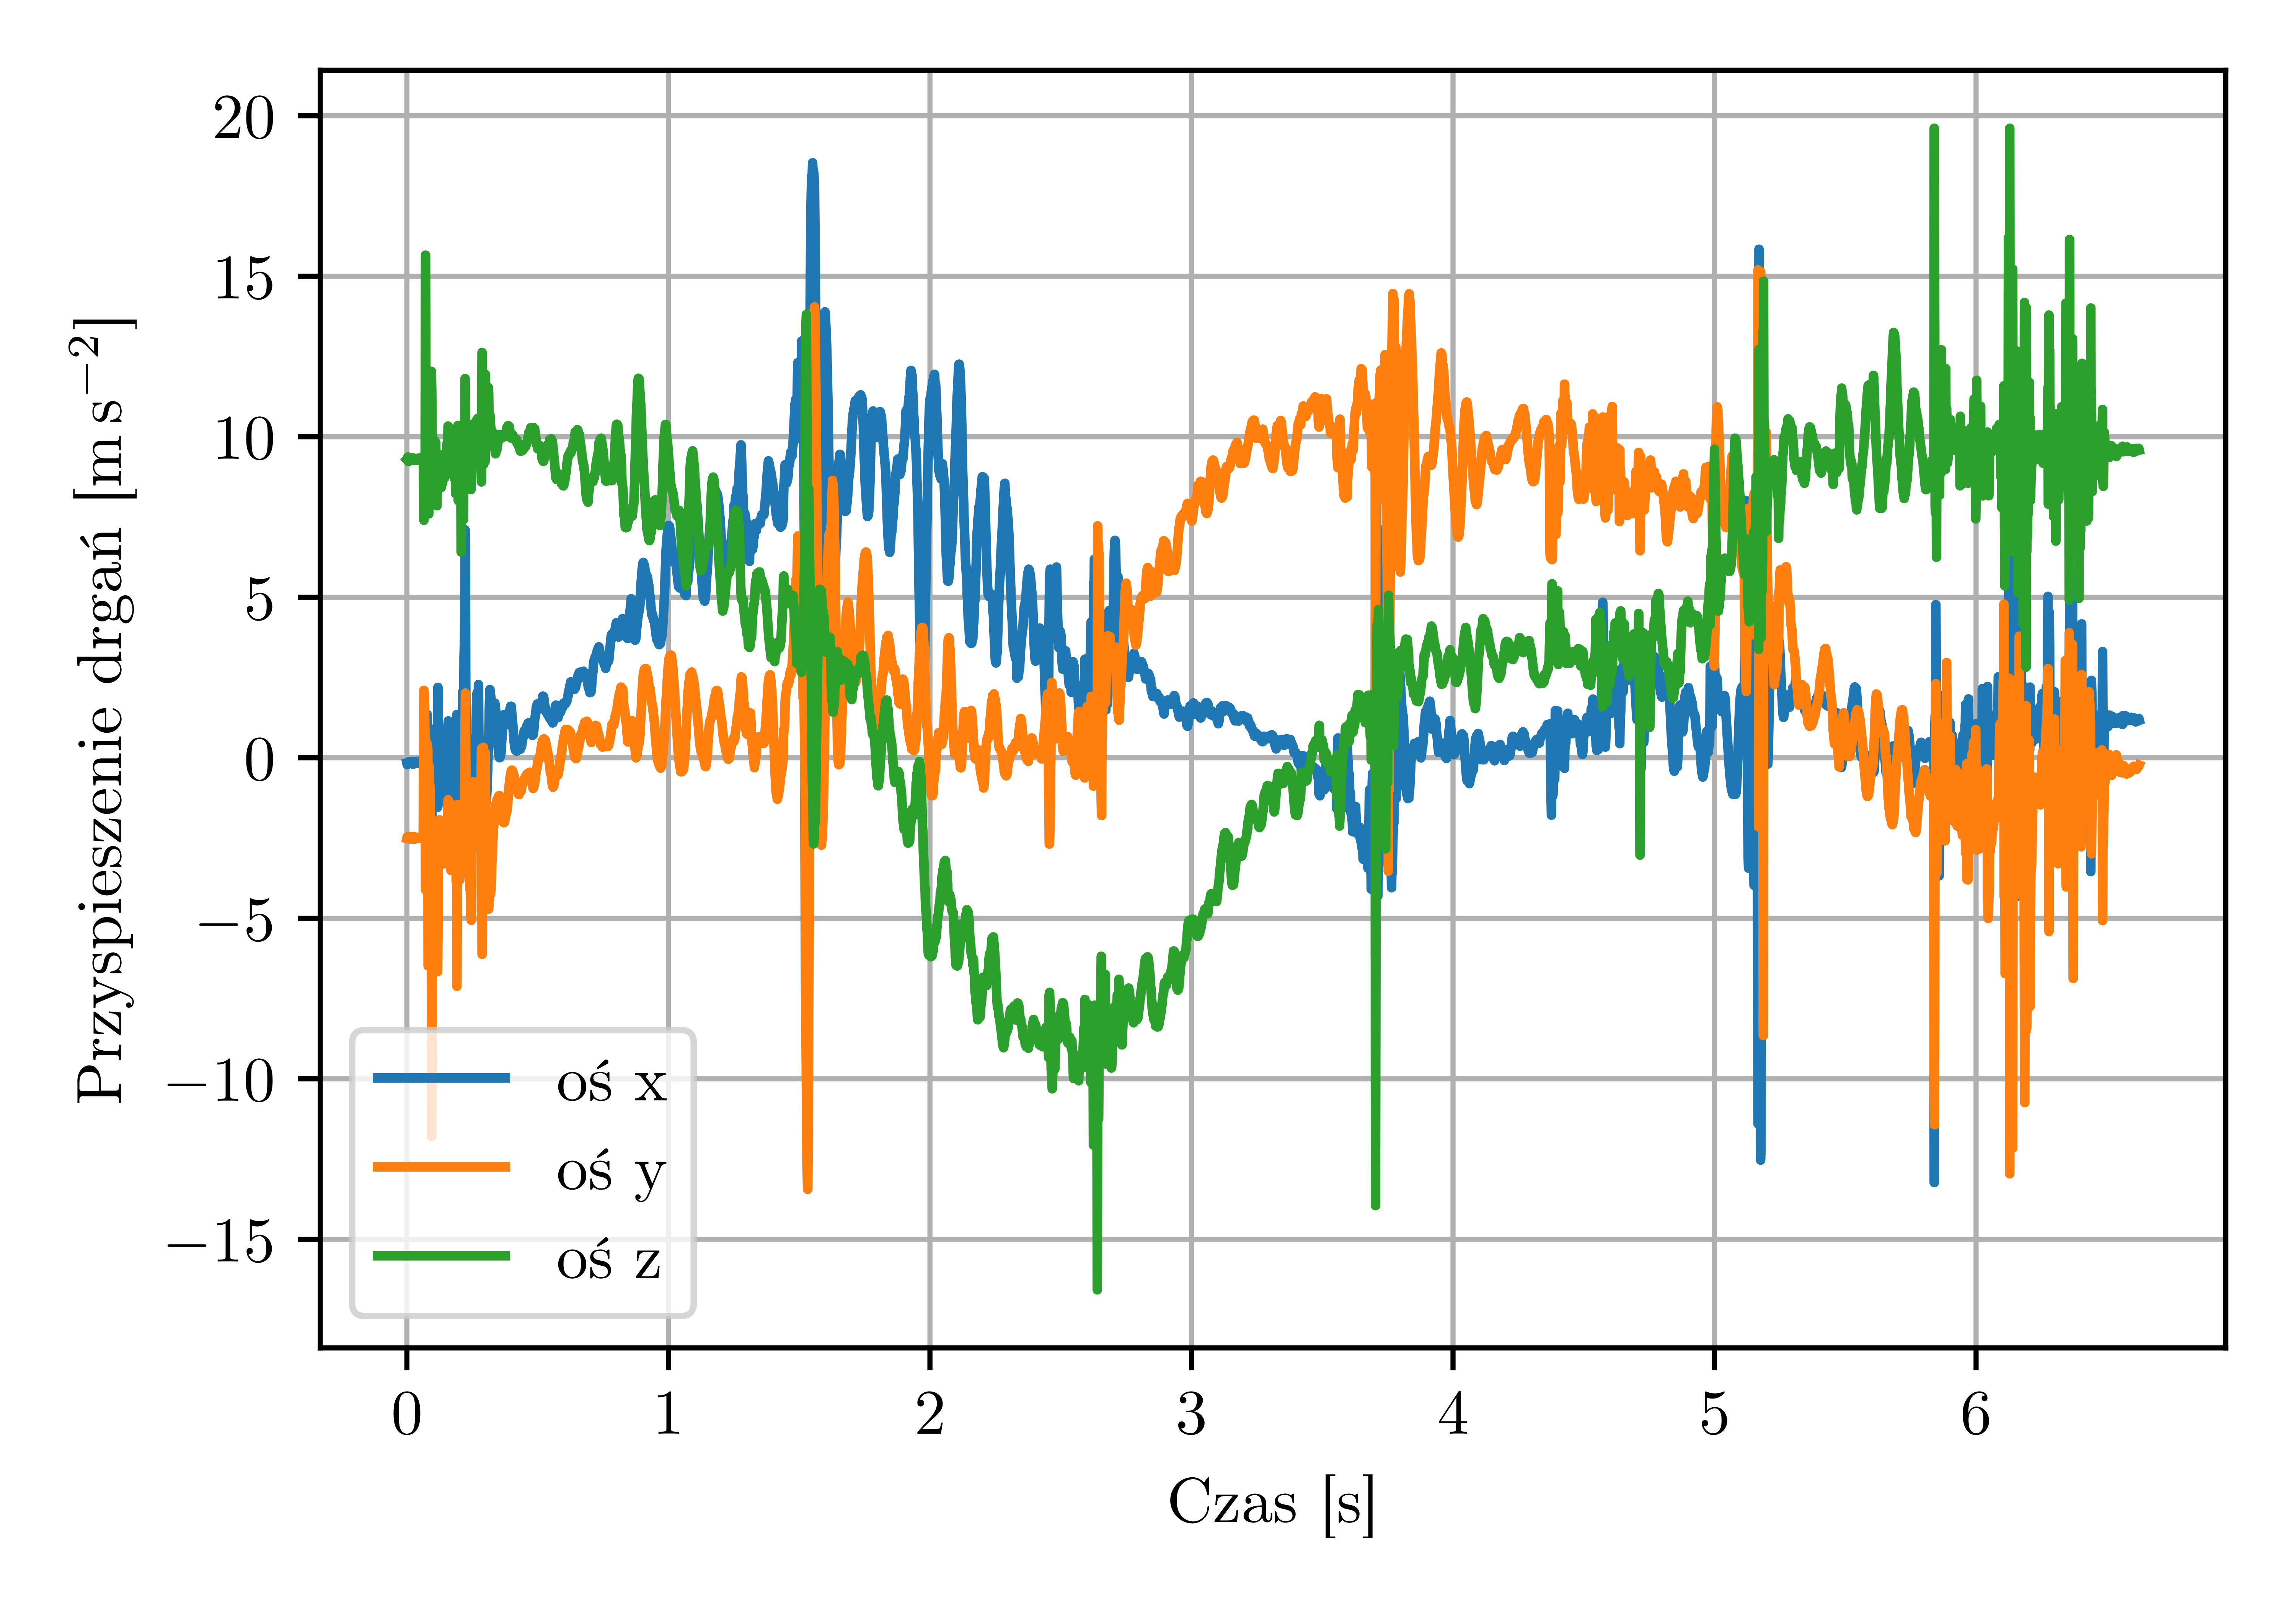
\includegraphics[width=0.8\textwidth]{plots/accel_2_xyz.png}',`
    %% Creator: Matplotlib, PGF backend
%%
%% To include the figure in your LaTeX document, write
%%   \input{<filename>.pgf}
%%
%% Make sure the required packages are loaded in your preamble
%%   \usepackage{pgf}
%%
%% Figures using additional raster images can only be included by \input if
%% they are in the same directory as the main LaTeX file. For loading figures
%% from other directories you can use the `import` package
%%   \usepackage{import}
%% and then include the figures with
%%   \import{<path to file>}{<filename>.pgf}
%%
%% Matplotlib used the following preamble
%%   \usepackage[utf8]{inputenc}
%%   \usepackage[T1]{fontenc}
%%   \usepackage{siunitx}
%%
\begingroup%
\makeatletter%
\begin{pgfpicture}%
\pgfpathrectangle{\pgfpointorigin}{\pgfqpoint{5.000000in}{3.500000in}}%
\pgfusepath{use as bounding box, clip}%
\begin{pgfscope}%
\pgfsetbuttcap%
\pgfsetmiterjoin%
\definecolor{currentfill}{rgb}{1.000000,1.000000,1.000000}%
\pgfsetfillcolor{currentfill}%
\pgfsetlinewidth{0.000000pt}%
\definecolor{currentstroke}{rgb}{1.000000,1.000000,1.000000}%
\pgfsetstrokecolor{currentstroke}%
\pgfsetdash{}{0pt}%
\pgfpathmoveto{\pgfqpoint{0.000000in}{0.000000in}}%
\pgfpathlineto{\pgfqpoint{5.000000in}{0.000000in}}%
\pgfpathlineto{\pgfqpoint{5.000000in}{3.500000in}}%
\pgfpathlineto{\pgfqpoint{0.000000in}{3.500000in}}%
\pgfpathclose%
\pgfusepath{fill}%
\end{pgfscope}%
\begin{pgfscope}%
\pgfsetbuttcap%
\pgfsetmiterjoin%
\definecolor{currentfill}{rgb}{1.000000,1.000000,1.000000}%
\pgfsetfillcolor{currentfill}%
\pgfsetlinewidth{0.000000pt}%
\definecolor{currentstroke}{rgb}{0.000000,0.000000,0.000000}%
\pgfsetstrokecolor{currentstroke}%
\pgfsetstrokeopacity{0.000000}%
\pgfsetdash{}{0pt}%
\pgfpathmoveto{\pgfqpoint{0.697462in}{0.564288in}}%
\pgfpathlineto{\pgfqpoint{4.815000in}{0.564288in}}%
\pgfpathlineto{\pgfqpoint{4.815000in}{3.315000in}}%
\pgfpathlineto{\pgfqpoint{0.697462in}{3.315000in}}%
\pgfpathclose%
\pgfusepath{fill}%
\end{pgfscope}%
\begin{pgfscope}%
\pgfpathrectangle{\pgfqpoint{0.697462in}{0.564288in}}{\pgfqpoint{4.117538in}{2.750712in}}%
\pgfusepath{clip}%
\pgfsetrectcap%
\pgfsetroundjoin%
\pgfsetlinewidth{0.803000pt}%
\definecolor{currentstroke}{rgb}{0.690196,0.690196,0.690196}%
\pgfsetstrokecolor{currentstroke}%
\pgfsetdash{}{0pt}%
\pgfpathmoveto{\pgfqpoint{1.025903in}{0.564288in}}%
\pgfpathlineto{\pgfqpoint{1.025903in}{3.315000in}}%
\pgfusepath{stroke}%
\end{pgfscope}%
\begin{pgfscope}%
\pgfsetbuttcap%
\pgfsetroundjoin%
\definecolor{currentfill}{rgb}{0.000000,0.000000,0.000000}%
\pgfsetfillcolor{currentfill}%
\pgfsetlinewidth{0.803000pt}%
\definecolor{currentstroke}{rgb}{0.000000,0.000000,0.000000}%
\pgfsetstrokecolor{currentstroke}%
\pgfsetdash{}{0pt}%
\pgfsys@defobject{currentmarker}{\pgfqpoint{0.000000in}{-0.048611in}}{\pgfqpoint{0.000000in}{0.000000in}}{%
\pgfpathmoveto{\pgfqpoint{0.000000in}{0.000000in}}%
\pgfpathlineto{\pgfqpoint{0.000000in}{-0.048611in}}%
\pgfusepath{stroke,fill}%
}%
\begin{pgfscope}%
\pgfsys@transformshift{1.025903in}{0.564288in}%
\pgfsys@useobject{currentmarker}{}%
\end{pgfscope}%
\end{pgfscope}%
\begin{pgfscope}%
\pgftext[x=1.025903in,y=0.467066in,,top]{\rmfamily\fontsize{10.000000}{12.000000}\selectfont \(\displaystyle 2\)}%
\end{pgfscope}%
\begin{pgfscope}%
\pgfpathrectangle{\pgfqpoint{0.697462in}{0.564288in}}{\pgfqpoint{4.117538in}{2.750712in}}%
\pgfusepath{clip}%
\pgfsetrectcap%
\pgfsetroundjoin%
\pgfsetlinewidth{0.803000pt}%
\definecolor{currentstroke}{rgb}{0.690196,0.690196,0.690196}%
\pgfsetstrokecolor{currentstroke}%
\pgfsetdash{}{0pt}%
\pgfpathmoveto{\pgfqpoint{1.591023in}{0.564288in}}%
\pgfpathlineto{\pgfqpoint{1.591023in}{3.315000in}}%
\pgfusepath{stroke}%
\end{pgfscope}%
\begin{pgfscope}%
\pgfsetbuttcap%
\pgfsetroundjoin%
\definecolor{currentfill}{rgb}{0.000000,0.000000,0.000000}%
\pgfsetfillcolor{currentfill}%
\pgfsetlinewidth{0.803000pt}%
\definecolor{currentstroke}{rgb}{0.000000,0.000000,0.000000}%
\pgfsetstrokecolor{currentstroke}%
\pgfsetdash{}{0pt}%
\pgfsys@defobject{currentmarker}{\pgfqpoint{0.000000in}{-0.048611in}}{\pgfqpoint{0.000000in}{0.000000in}}{%
\pgfpathmoveto{\pgfqpoint{0.000000in}{0.000000in}}%
\pgfpathlineto{\pgfqpoint{0.000000in}{-0.048611in}}%
\pgfusepath{stroke,fill}%
}%
\begin{pgfscope}%
\pgfsys@transformshift{1.591023in}{0.564288in}%
\pgfsys@useobject{currentmarker}{}%
\end{pgfscope}%
\end{pgfscope}%
\begin{pgfscope}%
\pgftext[x=1.591023in,y=0.467066in,,top]{\rmfamily\fontsize{10.000000}{12.000000}\selectfont \(\displaystyle 3\)}%
\end{pgfscope}%
\begin{pgfscope}%
\pgfpathrectangle{\pgfqpoint{0.697462in}{0.564288in}}{\pgfqpoint{4.117538in}{2.750712in}}%
\pgfusepath{clip}%
\pgfsetrectcap%
\pgfsetroundjoin%
\pgfsetlinewidth{0.803000pt}%
\definecolor{currentstroke}{rgb}{0.690196,0.690196,0.690196}%
\pgfsetstrokecolor{currentstroke}%
\pgfsetdash{}{0pt}%
\pgfpathmoveto{\pgfqpoint{2.156144in}{0.564288in}}%
\pgfpathlineto{\pgfqpoint{2.156144in}{3.315000in}}%
\pgfusepath{stroke}%
\end{pgfscope}%
\begin{pgfscope}%
\pgfsetbuttcap%
\pgfsetroundjoin%
\definecolor{currentfill}{rgb}{0.000000,0.000000,0.000000}%
\pgfsetfillcolor{currentfill}%
\pgfsetlinewidth{0.803000pt}%
\definecolor{currentstroke}{rgb}{0.000000,0.000000,0.000000}%
\pgfsetstrokecolor{currentstroke}%
\pgfsetdash{}{0pt}%
\pgfsys@defobject{currentmarker}{\pgfqpoint{0.000000in}{-0.048611in}}{\pgfqpoint{0.000000in}{0.000000in}}{%
\pgfpathmoveto{\pgfqpoint{0.000000in}{0.000000in}}%
\pgfpathlineto{\pgfqpoint{0.000000in}{-0.048611in}}%
\pgfusepath{stroke,fill}%
}%
\begin{pgfscope}%
\pgfsys@transformshift{2.156144in}{0.564288in}%
\pgfsys@useobject{currentmarker}{}%
\end{pgfscope}%
\end{pgfscope}%
\begin{pgfscope}%
\pgftext[x=2.156144in,y=0.467066in,,top]{\rmfamily\fontsize{10.000000}{12.000000}\selectfont \(\displaystyle 4\)}%
\end{pgfscope}%
\begin{pgfscope}%
\pgfpathrectangle{\pgfqpoint{0.697462in}{0.564288in}}{\pgfqpoint{4.117538in}{2.750712in}}%
\pgfusepath{clip}%
\pgfsetrectcap%
\pgfsetroundjoin%
\pgfsetlinewidth{0.803000pt}%
\definecolor{currentstroke}{rgb}{0.690196,0.690196,0.690196}%
\pgfsetstrokecolor{currentstroke}%
\pgfsetdash{}{0pt}%
\pgfpathmoveto{\pgfqpoint{2.721264in}{0.564288in}}%
\pgfpathlineto{\pgfqpoint{2.721264in}{3.315000in}}%
\pgfusepath{stroke}%
\end{pgfscope}%
\begin{pgfscope}%
\pgfsetbuttcap%
\pgfsetroundjoin%
\definecolor{currentfill}{rgb}{0.000000,0.000000,0.000000}%
\pgfsetfillcolor{currentfill}%
\pgfsetlinewidth{0.803000pt}%
\definecolor{currentstroke}{rgb}{0.000000,0.000000,0.000000}%
\pgfsetstrokecolor{currentstroke}%
\pgfsetdash{}{0pt}%
\pgfsys@defobject{currentmarker}{\pgfqpoint{0.000000in}{-0.048611in}}{\pgfqpoint{0.000000in}{0.000000in}}{%
\pgfpathmoveto{\pgfqpoint{0.000000in}{0.000000in}}%
\pgfpathlineto{\pgfqpoint{0.000000in}{-0.048611in}}%
\pgfusepath{stroke,fill}%
}%
\begin{pgfscope}%
\pgfsys@transformshift{2.721264in}{0.564288in}%
\pgfsys@useobject{currentmarker}{}%
\end{pgfscope}%
\end{pgfscope}%
\begin{pgfscope}%
\pgftext[x=2.721264in,y=0.467066in,,top]{\rmfamily\fontsize{10.000000}{12.000000}\selectfont \(\displaystyle 5\)}%
\end{pgfscope}%
\begin{pgfscope}%
\pgfpathrectangle{\pgfqpoint{0.697462in}{0.564288in}}{\pgfqpoint{4.117538in}{2.750712in}}%
\pgfusepath{clip}%
\pgfsetrectcap%
\pgfsetroundjoin%
\pgfsetlinewidth{0.803000pt}%
\definecolor{currentstroke}{rgb}{0.690196,0.690196,0.690196}%
\pgfsetstrokecolor{currentstroke}%
\pgfsetdash{}{0pt}%
\pgfpathmoveto{\pgfqpoint{3.286385in}{0.564288in}}%
\pgfpathlineto{\pgfqpoint{3.286385in}{3.315000in}}%
\pgfusepath{stroke}%
\end{pgfscope}%
\begin{pgfscope}%
\pgfsetbuttcap%
\pgfsetroundjoin%
\definecolor{currentfill}{rgb}{0.000000,0.000000,0.000000}%
\pgfsetfillcolor{currentfill}%
\pgfsetlinewidth{0.803000pt}%
\definecolor{currentstroke}{rgb}{0.000000,0.000000,0.000000}%
\pgfsetstrokecolor{currentstroke}%
\pgfsetdash{}{0pt}%
\pgfsys@defobject{currentmarker}{\pgfqpoint{0.000000in}{-0.048611in}}{\pgfqpoint{0.000000in}{0.000000in}}{%
\pgfpathmoveto{\pgfqpoint{0.000000in}{0.000000in}}%
\pgfpathlineto{\pgfqpoint{0.000000in}{-0.048611in}}%
\pgfusepath{stroke,fill}%
}%
\begin{pgfscope}%
\pgfsys@transformshift{3.286385in}{0.564288in}%
\pgfsys@useobject{currentmarker}{}%
\end{pgfscope}%
\end{pgfscope}%
\begin{pgfscope}%
\pgftext[x=3.286385in,y=0.467066in,,top]{\rmfamily\fontsize{10.000000}{12.000000}\selectfont \(\displaystyle 6\)}%
\end{pgfscope}%
\begin{pgfscope}%
\pgfpathrectangle{\pgfqpoint{0.697462in}{0.564288in}}{\pgfqpoint{4.117538in}{2.750712in}}%
\pgfusepath{clip}%
\pgfsetrectcap%
\pgfsetroundjoin%
\pgfsetlinewidth{0.803000pt}%
\definecolor{currentstroke}{rgb}{0.690196,0.690196,0.690196}%
\pgfsetstrokecolor{currentstroke}%
\pgfsetdash{}{0pt}%
\pgfpathmoveto{\pgfqpoint{3.851505in}{0.564288in}}%
\pgfpathlineto{\pgfqpoint{3.851505in}{3.315000in}}%
\pgfusepath{stroke}%
\end{pgfscope}%
\begin{pgfscope}%
\pgfsetbuttcap%
\pgfsetroundjoin%
\definecolor{currentfill}{rgb}{0.000000,0.000000,0.000000}%
\pgfsetfillcolor{currentfill}%
\pgfsetlinewidth{0.803000pt}%
\definecolor{currentstroke}{rgb}{0.000000,0.000000,0.000000}%
\pgfsetstrokecolor{currentstroke}%
\pgfsetdash{}{0pt}%
\pgfsys@defobject{currentmarker}{\pgfqpoint{0.000000in}{-0.048611in}}{\pgfqpoint{0.000000in}{0.000000in}}{%
\pgfpathmoveto{\pgfqpoint{0.000000in}{0.000000in}}%
\pgfpathlineto{\pgfqpoint{0.000000in}{-0.048611in}}%
\pgfusepath{stroke,fill}%
}%
\begin{pgfscope}%
\pgfsys@transformshift{3.851505in}{0.564288in}%
\pgfsys@useobject{currentmarker}{}%
\end{pgfscope}%
\end{pgfscope}%
\begin{pgfscope}%
\pgftext[x=3.851505in,y=0.467066in,,top]{\rmfamily\fontsize{10.000000}{12.000000}\selectfont \(\displaystyle 7\)}%
\end{pgfscope}%
\begin{pgfscope}%
\pgfpathrectangle{\pgfqpoint{0.697462in}{0.564288in}}{\pgfqpoint{4.117538in}{2.750712in}}%
\pgfusepath{clip}%
\pgfsetrectcap%
\pgfsetroundjoin%
\pgfsetlinewidth{0.803000pt}%
\definecolor{currentstroke}{rgb}{0.690196,0.690196,0.690196}%
\pgfsetstrokecolor{currentstroke}%
\pgfsetdash{}{0pt}%
\pgfpathmoveto{\pgfqpoint{4.416625in}{0.564288in}}%
\pgfpathlineto{\pgfqpoint{4.416625in}{3.315000in}}%
\pgfusepath{stroke}%
\end{pgfscope}%
\begin{pgfscope}%
\pgfsetbuttcap%
\pgfsetroundjoin%
\definecolor{currentfill}{rgb}{0.000000,0.000000,0.000000}%
\pgfsetfillcolor{currentfill}%
\pgfsetlinewidth{0.803000pt}%
\definecolor{currentstroke}{rgb}{0.000000,0.000000,0.000000}%
\pgfsetstrokecolor{currentstroke}%
\pgfsetdash{}{0pt}%
\pgfsys@defobject{currentmarker}{\pgfqpoint{0.000000in}{-0.048611in}}{\pgfqpoint{0.000000in}{0.000000in}}{%
\pgfpathmoveto{\pgfqpoint{0.000000in}{0.000000in}}%
\pgfpathlineto{\pgfqpoint{0.000000in}{-0.048611in}}%
\pgfusepath{stroke,fill}%
}%
\begin{pgfscope}%
\pgfsys@transformshift{4.416625in}{0.564288in}%
\pgfsys@useobject{currentmarker}{}%
\end{pgfscope}%
\end{pgfscope}%
\begin{pgfscope}%
\pgftext[x=4.416625in,y=0.467066in,,top]{\rmfamily\fontsize{10.000000}{12.000000}\selectfont \(\displaystyle 8\)}%
\end{pgfscope}%
\begin{pgfscope}%
\pgftext[x=2.756231in,y=0.288855in,,top]{\rmfamily\fontsize{10.000000}{12.000000}\selectfont Czas [\si{\second}]}%
\end{pgfscope}%
\begin{pgfscope}%
\pgfpathrectangle{\pgfqpoint{0.697462in}{0.564288in}}{\pgfqpoint{4.117538in}{2.750712in}}%
\pgfusepath{clip}%
\pgfsetrectcap%
\pgfsetroundjoin%
\pgfsetlinewidth{0.803000pt}%
\definecolor{currentstroke}{rgb}{0.690196,0.690196,0.690196}%
\pgfsetstrokecolor{currentstroke}%
\pgfsetdash{}{0pt}%
\pgfpathmoveto{\pgfqpoint{0.697462in}{0.798007in}}%
\pgfpathlineto{\pgfqpoint{4.815000in}{0.798007in}}%
\pgfusepath{stroke}%
\end{pgfscope}%
\begin{pgfscope}%
\pgfsetbuttcap%
\pgfsetroundjoin%
\definecolor{currentfill}{rgb}{0.000000,0.000000,0.000000}%
\pgfsetfillcolor{currentfill}%
\pgfsetlinewidth{0.803000pt}%
\definecolor{currentstroke}{rgb}{0.000000,0.000000,0.000000}%
\pgfsetstrokecolor{currentstroke}%
\pgfsetdash{}{0pt}%
\pgfsys@defobject{currentmarker}{\pgfqpoint{-0.048611in}{0.000000in}}{\pgfqpoint{0.000000in}{0.000000in}}{%
\pgfpathmoveto{\pgfqpoint{0.000000in}{0.000000in}}%
\pgfpathlineto{\pgfqpoint{-0.048611in}{0.000000in}}%
\pgfusepath{stroke,fill}%
}%
\begin{pgfscope}%
\pgfsys@transformshift{0.697462in}{0.798007in}%
\pgfsys@useobject{currentmarker}{}%
\end{pgfscope}%
\end{pgfscope}%
\begin{pgfscope}%
\pgftext[x=0.353325in,y=0.750179in,left,base]{\rmfamily\fontsize{10.000000}{12.000000}\selectfont \(\displaystyle -15\)}%
\end{pgfscope}%
\begin{pgfscope}%
\pgfpathrectangle{\pgfqpoint{0.697462in}{0.564288in}}{\pgfqpoint{4.117538in}{2.750712in}}%
\pgfusepath{clip}%
\pgfsetrectcap%
\pgfsetroundjoin%
\pgfsetlinewidth{0.803000pt}%
\definecolor{currentstroke}{rgb}{0.690196,0.690196,0.690196}%
\pgfsetstrokecolor{currentstroke}%
\pgfsetdash{}{0pt}%
\pgfpathmoveto{\pgfqpoint{0.697462in}{1.143557in}}%
\pgfpathlineto{\pgfqpoint{4.815000in}{1.143557in}}%
\pgfusepath{stroke}%
\end{pgfscope}%
\begin{pgfscope}%
\pgfsetbuttcap%
\pgfsetroundjoin%
\definecolor{currentfill}{rgb}{0.000000,0.000000,0.000000}%
\pgfsetfillcolor{currentfill}%
\pgfsetlinewidth{0.803000pt}%
\definecolor{currentstroke}{rgb}{0.000000,0.000000,0.000000}%
\pgfsetstrokecolor{currentstroke}%
\pgfsetdash{}{0pt}%
\pgfsys@defobject{currentmarker}{\pgfqpoint{-0.048611in}{0.000000in}}{\pgfqpoint{0.000000in}{0.000000in}}{%
\pgfpathmoveto{\pgfqpoint{0.000000in}{0.000000in}}%
\pgfpathlineto{\pgfqpoint{-0.048611in}{0.000000in}}%
\pgfusepath{stroke,fill}%
}%
\begin{pgfscope}%
\pgfsys@transformshift{0.697462in}{1.143557in}%
\pgfsys@useobject{currentmarker}{}%
\end{pgfscope}%
\end{pgfscope}%
\begin{pgfscope}%
\pgftext[x=0.353325in,y=1.095729in,left,base]{\rmfamily\fontsize{10.000000}{12.000000}\selectfont \(\displaystyle -10\)}%
\end{pgfscope}%
\begin{pgfscope}%
\pgfpathrectangle{\pgfqpoint{0.697462in}{0.564288in}}{\pgfqpoint{4.117538in}{2.750712in}}%
\pgfusepath{clip}%
\pgfsetrectcap%
\pgfsetroundjoin%
\pgfsetlinewidth{0.803000pt}%
\definecolor{currentstroke}{rgb}{0.690196,0.690196,0.690196}%
\pgfsetstrokecolor{currentstroke}%
\pgfsetdash{}{0pt}%
\pgfpathmoveto{\pgfqpoint{0.697462in}{1.489107in}}%
\pgfpathlineto{\pgfqpoint{4.815000in}{1.489107in}}%
\pgfusepath{stroke}%
\end{pgfscope}%
\begin{pgfscope}%
\pgfsetbuttcap%
\pgfsetroundjoin%
\definecolor{currentfill}{rgb}{0.000000,0.000000,0.000000}%
\pgfsetfillcolor{currentfill}%
\pgfsetlinewidth{0.803000pt}%
\definecolor{currentstroke}{rgb}{0.000000,0.000000,0.000000}%
\pgfsetstrokecolor{currentstroke}%
\pgfsetdash{}{0pt}%
\pgfsys@defobject{currentmarker}{\pgfqpoint{-0.048611in}{0.000000in}}{\pgfqpoint{0.000000in}{0.000000in}}{%
\pgfpathmoveto{\pgfqpoint{0.000000in}{0.000000in}}%
\pgfpathlineto{\pgfqpoint{-0.048611in}{0.000000in}}%
\pgfusepath{stroke,fill}%
}%
\begin{pgfscope}%
\pgfsys@transformshift{0.697462in}{1.489107in}%
\pgfsys@useobject{currentmarker}{}%
\end{pgfscope}%
\end{pgfscope}%
\begin{pgfscope}%
\pgftext[x=0.422770in,y=1.441280in,left,base]{\rmfamily\fontsize{10.000000}{12.000000}\selectfont \(\displaystyle -5\)}%
\end{pgfscope}%
\begin{pgfscope}%
\pgfpathrectangle{\pgfqpoint{0.697462in}{0.564288in}}{\pgfqpoint{4.117538in}{2.750712in}}%
\pgfusepath{clip}%
\pgfsetrectcap%
\pgfsetroundjoin%
\pgfsetlinewidth{0.803000pt}%
\definecolor{currentstroke}{rgb}{0.690196,0.690196,0.690196}%
\pgfsetstrokecolor{currentstroke}%
\pgfsetdash{}{0pt}%
\pgfpathmoveto{\pgfqpoint{0.697462in}{1.834657in}}%
\pgfpathlineto{\pgfqpoint{4.815000in}{1.834657in}}%
\pgfusepath{stroke}%
\end{pgfscope}%
\begin{pgfscope}%
\pgfsetbuttcap%
\pgfsetroundjoin%
\definecolor{currentfill}{rgb}{0.000000,0.000000,0.000000}%
\pgfsetfillcolor{currentfill}%
\pgfsetlinewidth{0.803000pt}%
\definecolor{currentstroke}{rgb}{0.000000,0.000000,0.000000}%
\pgfsetstrokecolor{currentstroke}%
\pgfsetdash{}{0pt}%
\pgfsys@defobject{currentmarker}{\pgfqpoint{-0.048611in}{0.000000in}}{\pgfqpoint{0.000000in}{0.000000in}}{%
\pgfpathmoveto{\pgfqpoint{0.000000in}{0.000000in}}%
\pgfpathlineto{\pgfqpoint{-0.048611in}{0.000000in}}%
\pgfusepath{stroke,fill}%
}%
\begin{pgfscope}%
\pgfsys@transformshift{0.697462in}{1.834657in}%
\pgfsys@useobject{currentmarker}{}%
\end{pgfscope}%
\end{pgfscope}%
\begin{pgfscope}%
\pgftext[x=0.530795in,y=1.786830in,left,base]{\rmfamily\fontsize{10.000000}{12.000000}\selectfont \(\displaystyle 0\)}%
\end{pgfscope}%
\begin{pgfscope}%
\pgfpathrectangle{\pgfqpoint{0.697462in}{0.564288in}}{\pgfqpoint{4.117538in}{2.750712in}}%
\pgfusepath{clip}%
\pgfsetrectcap%
\pgfsetroundjoin%
\pgfsetlinewidth{0.803000pt}%
\definecolor{currentstroke}{rgb}{0.690196,0.690196,0.690196}%
\pgfsetstrokecolor{currentstroke}%
\pgfsetdash{}{0pt}%
\pgfpathmoveto{\pgfqpoint{0.697462in}{2.180208in}}%
\pgfpathlineto{\pgfqpoint{4.815000in}{2.180208in}}%
\pgfusepath{stroke}%
\end{pgfscope}%
\begin{pgfscope}%
\pgfsetbuttcap%
\pgfsetroundjoin%
\definecolor{currentfill}{rgb}{0.000000,0.000000,0.000000}%
\pgfsetfillcolor{currentfill}%
\pgfsetlinewidth{0.803000pt}%
\definecolor{currentstroke}{rgb}{0.000000,0.000000,0.000000}%
\pgfsetstrokecolor{currentstroke}%
\pgfsetdash{}{0pt}%
\pgfsys@defobject{currentmarker}{\pgfqpoint{-0.048611in}{0.000000in}}{\pgfqpoint{0.000000in}{0.000000in}}{%
\pgfpathmoveto{\pgfqpoint{0.000000in}{0.000000in}}%
\pgfpathlineto{\pgfqpoint{-0.048611in}{0.000000in}}%
\pgfusepath{stroke,fill}%
}%
\begin{pgfscope}%
\pgfsys@transformshift{0.697462in}{2.180208in}%
\pgfsys@useobject{currentmarker}{}%
\end{pgfscope}%
\end{pgfscope}%
\begin{pgfscope}%
\pgftext[x=0.530795in,y=2.132380in,left,base]{\rmfamily\fontsize{10.000000}{12.000000}\selectfont \(\displaystyle 5\)}%
\end{pgfscope}%
\begin{pgfscope}%
\pgfpathrectangle{\pgfqpoint{0.697462in}{0.564288in}}{\pgfqpoint{4.117538in}{2.750712in}}%
\pgfusepath{clip}%
\pgfsetrectcap%
\pgfsetroundjoin%
\pgfsetlinewidth{0.803000pt}%
\definecolor{currentstroke}{rgb}{0.690196,0.690196,0.690196}%
\pgfsetstrokecolor{currentstroke}%
\pgfsetdash{}{0pt}%
\pgfpathmoveto{\pgfqpoint{0.697462in}{2.525758in}}%
\pgfpathlineto{\pgfqpoint{4.815000in}{2.525758in}}%
\pgfusepath{stroke}%
\end{pgfscope}%
\begin{pgfscope}%
\pgfsetbuttcap%
\pgfsetroundjoin%
\definecolor{currentfill}{rgb}{0.000000,0.000000,0.000000}%
\pgfsetfillcolor{currentfill}%
\pgfsetlinewidth{0.803000pt}%
\definecolor{currentstroke}{rgb}{0.000000,0.000000,0.000000}%
\pgfsetstrokecolor{currentstroke}%
\pgfsetdash{}{0pt}%
\pgfsys@defobject{currentmarker}{\pgfqpoint{-0.048611in}{0.000000in}}{\pgfqpoint{0.000000in}{0.000000in}}{%
\pgfpathmoveto{\pgfqpoint{0.000000in}{0.000000in}}%
\pgfpathlineto{\pgfqpoint{-0.048611in}{0.000000in}}%
\pgfusepath{stroke,fill}%
}%
\begin{pgfscope}%
\pgfsys@transformshift{0.697462in}{2.525758in}%
\pgfsys@useobject{currentmarker}{}%
\end{pgfscope}%
\end{pgfscope}%
\begin{pgfscope}%
\pgftext[x=0.461350in,y=2.477930in,left,base]{\rmfamily\fontsize{10.000000}{12.000000}\selectfont \(\displaystyle 10\)}%
\end{pgfscope}%
\begin{pgfscope}%
\pgfpathrectangle{\pgfqpoint{0.697462in}{0.564288in}}{\pgfqpoint{4.117538in}{2.750712in}}%
\pgfusepath{clip}%
\pgfsetrectcap%
\pgfsetroundjoin%
\pgfsetlinewidth{0.803000pt}%
\definecolor{currentstroke}{rgb}{0.690196,0.690196,0.690196}%
\pgfsetstrokecolor{currentstroke}%
\pgfsetdash{}{0pt}%
\pgfpathmoveto{\pgfqpoint{0.697462in}{2.871308in}}%
\pgfpathlineto{\pgfqpoint{4.815000in}{2.871308in}}%
\pgfusepath{stroke}%
\end{pgfscope}%
\begin{pgfscope}%
\pgfsetbuttcap%
\pgfsetroundjoin%
\definecolor{currentfill}{rgb}{0.000000,0.000000,0.000000}%
\pgfsetfillcolor{currentfill}%
\pgfsetlinewidth{0.803000pt}%
\definecolor{currentstroke}{rgb}{0.000000,0.000000,0.000000}%
\pgfsetstrokecolor{currentstroke}%
\pgfsetdash{}{0pt}%
\pgfsys@defobject{currentmarker}{\pgfqpoint{-0.048611in}{0.000000in}}{\pgfqpoint{0.000000in}{0.000000in}}{%
\pgfpathmoveto{\pgfqpoint{0.000000in}{0.000000in}}%
\pgfpathlineto{\pgfqpoint{-0.048611in}{0.000000in}}%
\pgfusepath{stroke,fill}%
}%
\begin{pgfscope}%
\pgfsys@transformshift{0.697462in}{2.871308in}%
\pgfsys@useobject{currentmarker}{}%
\end{pgfscope}%
\end{pgfscope}%
\begin{pgfscope}%
\pgftext[x=0.461350in,y=2.823480in,left,base]{\rmfamily\fontsize{10.000000}{12.000000}\selectfont \(\displaystyle 15\)}%
\end{pgfscope}%
\begin{pgfscope}%
\pgfpathrectangle{\pgfqpoint{0.697462in}{0.564288in}}{\pgfqpoint{4.117538in}{2.750712in}}%
\pgfusepath{clip}%
\pgfsetrectcap%
\pgfsetroundjoin%
\pgfsetlinewidth{0.803000pt}%
\definecolor{currentstroke}{rgb}{0.690196,0.690196,0.690196}%
\pgfsetstrokecolor{currentstroke}%
\pgfsetdash{}{0pt}%
\pgfpathmoveto{\pgfqpoint{0.697462in}{3.216858in}}%
\pgfpathlineto{\pgfqpoint{4.815000in}{3.216858in}}%
\pgfusepath{stroke}%
\end{pgfscope}%
\begin{pgfscope}%
\pgfsetbuttcap%
\pgfsetroundjoin%
\definecolor{currentfill}{rgb}{0.000000,0.000000,0.000000}%
\pgfsetfillcolor{currentfill}%
\pgfsetlinewidth{0.803000pt}%
\definecolor{currentstroke}{rgb}{0.000000,0.000000,0.000000}%
\pgfsetstrokecolor{currentstroke}%
\pgfsetdash{}{0pt}%
\pgfsys@defobject{currentmarker}{\pgfqpoint{-0.048611in}{0.000000in}}{\pgfqpoint{0.000000in}{0.000000in}}{%
\pgfpathmoveto{\pgfqpoint{0.000000in}{0.000000in}}%
\pgfpathlineto{\pgfqpoint{-0.048611in}{0.000000in}}%
\pgfusepath{stroke,fill}%
}%
\begin{pgfscope}%
\pgfsys@transformshift{0.697462in}{3.216858in}%
\pgfsys@useobject{currentmarker}{}%
\end{pgfscope}%
\end{pgfscope}%
\begin{pgfscope}%
\pgftext[x=0.461350in,y=3.169030in,left,base]{\rmfamily\fontsize{10.000000}{12.000000}\selectfont \(\displaystyle 20\)}%
\end{pgfscope}%
\begin{pgfscope}%
\pgftext[x=0.297770in,y=1.939644in,,bottom,rotate=90.000000]{\rmfamily\fontsize{10.000000}{12.000000}\selectfont Przyspieszenie drgań [\si{\meter\per\second\squared}]}%
\end{pgfscope}%
\begin{pgfscope}%
\pgfpathrectangle{\pgfqpoint{0.697462in}{0.564288in}}{\pgfqpoint{4.117538in}{2.750712in}}%
\pgfusepath{clip}%
\pgfsetrectcap%
\pgfsetroundjoin%
\pgfsetlinewidth{1.505625pt}%
\definecolor{currentstroke}{rgb}{0.121569,0.466667,0.705882}%
\pgfsetstrokecolor{currentstroke}%
\pgfsetdash{}{0pt}%
\pgfpathmoveto{\pgfqpoint{0.884623in}{1.823406in}}%
\pgfpathlineto{\pgfqpoint{0.885329in}{1.820097in}}%
\pgfpathlineto{\pgfqpoint{0.886035in}{1.825061in}}%
\pgfpathlineto{\pgfqpoint{0.886742in}{1.823737in}}%
\pgfpathlineto{\pgfqpoint{0.889567in}{1.826053in}}%
\pgfpathlineto{\pgfqpoint{0.890980in}{1.824730in}}%
\pgfpathlineto{\pgfqpoint{0.891687in}{1.826384in}}%
\pgfpathlineto{\pgfqpoint{0.892393in}{1.822413in}}%
\pgfpathlineto{\pgfqpoint{0.893099in}{1.823075in}}%
\pgfpathlineto{\pgfqpoint{0.894512in}{1.824399in}}%
\pgfpathlineto{\pgfqpoint{0.895219in}{1.823075in}}%
\pgfpathlineto{\pgfqpoint{0.895925in}{1.824068in}}%
\pgfpathlineto{\pgfqpoint{0.896631in}{1.826715in}}%
\pgfpathlineto{\pgfqpoint{0.897338in}{1.821089in}}%
\pgfpathlineto{\pgfqpoint{0.898044in}{1.822744in}}%
\pgfpathlineto{\pgfqpoint{0.898751in}{1.821089in}}%
\pgfpathlineto{\pgfqpoint{0.900870in}{1.826715in}}%
\pgfpathlineto{\pgfqpoint{0.901576in}{1.824399in}}%
\pgfpathlineto{\pgfqpoint{0.902283in}{1.824730in}}%
\pgfpathlineto{\pgfqpoint{0.902989in}{1.826053in}}%
\pgfpathlineto{\pgfqpoint{0.903695in}{1.823406in}}%
\pgfpathlineto{\pgfqpoint{0.904402in}{1.824399in}}%
\pgfpathlineto{\pgfqpoint{0.905815in}{1.826715in}}%
\pgfpathlineto{\pgfqpoint{0.906521in}{1.823406in}}%
\pgfpathlineto{\pgfqpoint{0.907227in}{1.825722in}}%
\pgfpathlineto{\pgfqpoint{0.907934in}{1.825061in}}%
\pgfpathlineto{\pgfqpoint{0.908640in}{1.822744in}}%
\pgfpathlineto{\pgfqpoint{0.909347in}{1.824399in}}%
\pgfpathlineto{\pgfqpoint{0.910053in}{1.823737in}}%
\pgfpathlineto{\pgfqpoint{0.910759in}{1.824068in}}%
\pgfpathlineto{\pgfqpoint{0.911466in}{1.822082in}}%
\pgfpathlineto{\pgfqpoint{0.912172in}{1.823075in}}%
\pgfpathlineto{\pgfqpoint{0.912879in}{1.828039in}}%
\pgfpathlineto{\pgfqpoint{0.913585in}{1.823406in}}%
\pgfpathlineto{\pgfqpoint{0.914291in}{1.824399in}}%
\pgfpathlineto{\pgfqpoint{0.915704in}{1.825722in}}%
\pgfpathlineto{\pgfqpoint{0.917117in}{1.823075in}}%
\pgfpathlineto{\pgfqpoint{0.919236in}{1.824399in}}%
\pgfpathlineto{\pgfqpoint{0.919943in}{1.821420in}}%
\pgfpathlineto{\pgfqpoint{0.920649in}{1.826384in}}%
\pgfpathlineto{\pgfqpoint{0.921355in}{1.847895in}}%
\pgfpathlineto{\pgfqpoint{0.923475in}{1.790313in}}%
\pgfpathlineto{\pgfqpoint{0.924181in}{1.820097in}}%
\pgfpathlineto{\pgfqpoint{0.924887in}{1.765494in}}%
\pgfpathlineto{\pgfqpoint{0.926300in}{1.872052in}}%
\pgfpathlineto{\pgfqpoint{0.927007in}{1.862124in}}%
\pgfpathlineto{\pgfqpoint{0.928419in}{1.927979in}}%
\pgfpathlineto{\pgfqpoint{0.929832in}{1.833334in}}%
\pgfpathlineto{\pgfqpoint{0.930539in}{1.896872in}}%
\pgfpathlineto{\pgfqpoint{0.931245in}{1.725121in}}%
\pgfpathlineto{\pgfqpoint{0.931951in}{1.814471in}}%
\pgfpathlineto{\pgfqpoint{0.932658in}{1.894555in}}%
\pgfpathlineto{\pgfqpoint{0.934071in}{1.766818in}}%
\pgfpathlineto{\pgfqpoint{0.934777in}{1.897534in}}%
\pgfpathlineto{\pgfqpoint{0.935483in}{1.764501in}}%
\pgfpathlineto{\pgfqpoint{0.936190in}{1.821420in}}%
\pgfpathlineto{\pgfqpoint{0.936896in}{1.766156in}}%
\pgfpathlineto{\pgfqpoint{0.937603in}{1.526896in}}%
\pgfpathlineto{\pgfqpoint{0.939722in}{1.765825in}}%
\pgfpathlineto{\pgfqpoint{0.940428in}{1.771120in}}%
\pgfpathlineto{\pgfqpoint{0.941135in}{1.768803in}}%
\pgfpathlineto{\pgfqpoint{0.941841in}{1.799248in}}%
\pgfpathlineto{\pgfqpoint{0.942547in}{1.793953in}}%
\pgfpathlineto{\pgfqpoint{0.943960in}{1.755566in}}%
\pgfpathlineto{\pgfqpoint{0.944667in}{1.787004in}}%
\pgfpathlineto{\pgfqpoint{0.945373in}{1.765163in}}%
\pgfpathlineto{\pgfqpoint{0.946786in}{1.818773in}}%
\pgfpathlineto{\pgfqpoint{0.947492in}{1.758544in}}%
\pgfpathlineto{\pgfqpoint{0.948199in}{1.804543in}}%
\pgfpathlineto{\pgfqpoint{0.948905in}{1.778731in}}%
\pgfpathlineto{\pgfqpoint{0.949611in}{1.798586in}}%
\pgfpathlineto{\pgfqpoint{0.950318in}{1.727768in}}%
\pgfpathlineto{\pgfqpoint{0.951731in}{1.986222in}}%
\pgfpathlineto{\pgfqpoint{0.955263in}{1.770789in}}%
\pgfpathlineto{\pgfqpoint{0.955969in}{1.765163in}}%
\pgfpathlineto{\pgfqpoint{0.956675in}{1.748286in}}%
\pgfpathlineto{\pgfqpoint{0.957382in}{1.753580in}}%
\pgfpathlineto{\pgfqpoint{0.959501in}{1.789651in}}%
\pgfpathlineto{\pgfqpoint{0.960914in}{1.893893in}}%
\pgfpathlineto{\pgfqpoint{0.961620in}{1.823737in}}%
\pgfpathlineto{\pgfqpoint{0.962327in}{1.853851in}}%
\pgfpathlineto{\pgfqpoint{0.963033in}{1.882973in}}%
\pgfpathlineto{\pgfqpoint{0.964446in}{1.771450in}}%
\pgfpathlineto{\pgfqpoint{0.965152in}{1.794946in}}%
\pgfpathlineto{\pgfqpoint{0.965859in}{1.801565in}}%
\pgfpathlineto{\pgfqpoint{0.967271in}{1.746962in}}%
\pgfpathlineto{\pgfqpoint{0.967978in}{1.757552in}}%
\pgfpathlineto{\pgfqpoint{0.970097in}{1.822082in}}%
\pgfpathlineto{\pgfqpoint{0.970804in}{1.816457in}}%
\pgfpathlineto{\pgfqpoint{0.971510in}{1.731408in}}%
\pgfpathlineto{\pgfqpoint{0.972216in}{1.775091in}}%
\pgfpathlineto{\pgfqpoint{0.973629in}{1.907130in}}%
\pgfpathlineto{\pgfqpoint{0.974336in}{1.914080in}}%
\pgfpathlineto{\pgfqpoint{0.976455in}{1.697654in}}%
\pgfpathlineto{\pgfqpoint{0.977161in}{1.722804in}}%
\pgfpathlineto{\pgfqpoint{0.977868in}{1.766156in}}%
\pgfpathlineto{\pgfqpoint{0.978574in}{1.704603in}}%
\pgfpathlineto{\pgfqpoint{0.979280in}{1.737696in}}%
\pgfpathlineto{\pgfqpoint{0.979987in}{1.825722in}}%
\pgfpathlineto{\pgfqpoint{0.980693in}{1.811162in}}%
\pgfpathlineto{\pgfqpoint{0.981400in}{1.808183in}}%
\pgfpathlineto{\pgfqpoint{0.982106in}{1.798917in}}%
\pgfpathlineto{\pgfqpoint{0.982812in}{1.799579in}}%
\pgfpathlineto{\pgfqpoint{0.983519in}{1.801234in}}%
\pgfpathlineto{\pgfqpoint{0.984932in}{1.709898in}}%
\pgfpathlineto{\pgfqpoint{0.987757in}{1.840614in}}%
\pgfpathlineto{\pgfqpoint{0.989170in}{1.865103in}}%
\pgfpathlineto{\pgfqpoint{0.990583in}{1.804543in}}%
\pgfpathlineto{\pgfqpoint{0.991289in}{1.808514in}}%
\pgfpathlineto{\pgfqpoint{0.991996in}{1.828039in}}%
\pgfpathlineto{\pgfqpoint{0.992702in}{1.927979in}}%
\pgfpathlineto{\pgfqpoint{0.994115in}{1.759206in}}%
\pgfpathlineto{\pgfqpoint{0.994821in}{1.801565in}}%
\pgfpathlineto{\pgfqpoint{0.995528in}{1.804874in}}%
\pgfpathlineto{\pgfqpoint{0.996234in}{1.752919in}}%
\pgfpathlineto{\pgfqpoint{0.996940in}{1.772774in}}%
\pgfpathlineto{\pgfqpoint{0.997647in}{1.804212in}}%
\pgfpathlineto{\pgfqpoint{0.998353in}{1.795939in}}%
\pgfpathlineto{\pgfqpoint{1.001885in}{1.737365in}}%
\pgfpathlineto{\pgfqpoint{1.004004in}{1.861463in}}%
\pgfpathlineto{\pgfqpoint{1.004711in}{1.837967in}}%
\pgfpathlineto{\pgfqpoint{1.005417in}{1.977287in}}%
\pgfpathlineto{\pgfqpoint{1.006830in}{1.785349in}}%
\pgfpathlineto{\pgfqpoint{1.008949in}{2.084176in}}%
\pgfpathlineto{\pgfqpoint{1.009656in}{2.143743in}}%
\pgfpathlineto{\pgfqpoint{1.010362in}{2.325422in}}%
\pgfpathlineto{\pgfqpoint{1.011068in}{2.272143in}}%
\pgfpathlineto{\pgfqpoint{1.013188in}{1.816457in}}%
\pgfpathlineto{\pgfqpoint{1.018839in}{1.872383in}}%
\pgfpathlineto{\pgfqpoint{1.020252in}{1.785018in}}%
\pgfpathlineto{\pgfqpoint{1.020958in}{1.793623in}}%
\pgfpathlineto{\pgfqpoint{1.021664in}{1.824730in}}%
\pgfpathlineto{\pgfqpoint{1.022371in}{1.818442in}}%
\pgfpathlineto{\pgfqpoint{1.023077in}{1.829363in}}%
\pgfpathlineto{\pgfqpoint{1.023784in}{1.812485in}}%
\pgfpathlineto{\pgfqpoint{1.025196in}{1.873707in}}%
\pgfpathlineto{\pgfqpoint{1.025903in}{1.875031in}}%
\pgfpathlineto{\pgfqpoint{1.027316in}{1.833996in}}%
\pgfpathlineto{\pgfqpoint{1.028728in}{1.794946in}}%
\pgfpathlineto{\pgfqpoint{1.029435in}{1.793623in}}%
\pgfpathlineto{\pgfqpoint{1.030141in}{1.799248in}}%
\pgfpathlineto{\pgfqpoint{1.031554in}{1.786011in}}%
\pgfpathlineto{\pgfqpoint{1.032260in}{1.789321in}}%
\pgfpathlineto{\pgfqpoint{1.033673in}{1.836643in}}%
\pgfpathlineto{\pgfqpoint{1.035792in}{1.970668in}}%
\pgfpathlineto{\pgfqpoint{1.036499in}{1.974970in}}%
\pgfpathlineto{\pgfqpoint{1.037205in}{1.946511in}}%
\pgfpathlineto{\pgfqpoint{1.037912in}{1.953460in}}%
\pgfpathlineto{\pgfqpoint{1.038618in}{1.937245in}}%
\pgfpathlineto{\pgfqpoint{1.039324in}{1.992179in}}%
\pgfpathlineto{\pgfqpoint{1.040737in}{1.844585in}}%
\pgfpathlineto{\pgfqpoint{1.042150in}{1.871390in}}%
\pgfpathlineto{\pgfqpoint{1.042856in}{1.858153in}}%
\pgfpathlineto{\pgfqpoint{1.043563in}{1.873045in}}%
\pgfpathlineto{\pgfqpoint{1.044269in}{1.869405in}}%
\pgfpathlineto{\pgfqpoint{1.044976in}{1.802227in}}%
\pgfpathlineto{\pgfqpoint{1.045682in}{1.844585in}}%
\pgfpathlineto{\pgfqpoint{1.047095in}{1.749278in}}%
\pgfpathlineto{\pgfqpoint{1.047801in}{1.805205in}}%
\pgfpathlineto{\pgfqpoint{1.048508in}{1.800572in}}%
\pgfpathlineto{\pgfqpoint{1.049920in}{1.846571in}}%
\pgfpathlineto{\pgfqpoint{1.050627in}{1.727768in}}%
\pgfpathlineto{\pgfqpoint{1.051333in}{1.731408in}}%
\pgfpathlineto{\pgfqpoint{1.052040in}{1.741998in}}%
\pgfpathlineto{\pgfqpoint{1.052746in}{1.717509in}}%
\pgfpathlineto{\pgfqpoint{1.053452in}{1.760861in}}%
\pgfpathlineto{\pgfqpoint{1.054159in}{1.677798in}}%
\pgfpathlineto{\pgfqpoint{1.054865in}{1.740343in}}%
\pgfpathlineto{\pgfqpoint{1.055572in}{1.736041in}}%
\pgfpathlineto{\pgfqpoint{1.056278in}{1.739682in}}%
\pgfpathlineto{\pgfqpoint{1.059104in}{1.807852in}}%
\pgfpathlineto{\pgfqpoint{1.063342in}{1.965704in}}%
\pgfpathlineto{\pgfqpoint{1.064048in}{1.981589in}}%
\pgfpathlineto{\pgfqpoint{1.064755in}{1.975963in}}%
\pgfpathlineto{\pgfqpoint{1.067580in}{1.939892in}}%
\pgfpathlineto{\pgfqpoint{1.069700in}{1.915404in}}%
\pgfpathlineto{\pgfqpoint{1.070406in}{1.916727in}}%
\pgfpathlineto{\pgfqpoint{1.073938in}{1.947503in}}%
\pgfpathlineto{\pgfqpoint{1.074644in}{1.952467in}}%
\pgfpathlineto{\pgfqpoint{1.076057in}{1.941216in}}%
\pgfpathlineto{\pgfqpoint{1.078883in}{1.898857in}}%
\pgfpathlineto{\pgfqpoint{1.084534in}{1.834988in}}%
\pgfpathlineto{\pgfqpoint{1.085240in}{1.834988in}}%
\pgfpathlineto{\pgfqpoint{1.087360in}{1.840945in}}%
\pgfpathlineto{\pgfqpoint{1.089479in}{1.869405in}}%
\pgfpathlineto{\pgfqpoint{1.093011in}{1.914742in}}%
\pgfpathlineto{\pgfqpoint{1.095130in}{1.927979in}}%
\pgfpathlineto{\pgfqpoint{1.095836in}{1.927979in}}%
\pgfpathlineto{\pgfqpoint{1.098662in}{1.919044in}}%
\pgfpathlineto{\pgfqpoint{1.100075in}{1.908785in}}%
\pgfpathlineto{\pgfqpoint{1.100781in}{1.909116in}}%
\pgfpathlineto{\pgfqpoint{1.101488in}{1.907130in}}%
\pgfpathlineto{\pgfqpoint{1.102194in}{1.907792in}}%
\pgfpathlineto{\pgfqpoint{1.103607in}{1.913418in}}%
\pgfpathlineto{\pgfqpoint{1.106432in}{1.935259in}}%
\pgfpathlineto{\pgfqpoint{1.109964in}{1.945518in}}%
\pgfpathlineto{\pgfqpoint{1.113496in}{1.905476in}}%
\pgfpathlineto{\pgfqpoint{1.117735in}{1.856499in}}%
\pgfpathlineto{\pgfqpoint{1.120560in}{1.850211in}}%
\pgfpathlineto{\pgfqpoint{1.121267in}{1.851204in}}%
\pgfpathlineto{\pgfqpoint{1.121973in}{1.849218in}}%
\pgfpathlineto{\pgfqpoint{1.124799in}{1.856830in}}%
\pgfpathlineto{\pgfqpoint{1.126918in}{1.852197in}}%
\pgfpathlineto{\pgfqpoint{1.127624in}{1.854182in}}%
\pgfpathlineto{\pgfqpoint{1.128331in}{1.853851in}}%
\pgfpathlineto{\pgfqpoint{1.129744in}{1.853189in}}%
\pgfpathlineto{\pgfqpoint{1.133982in}{1.869736in}}%
\pgfpathlineto{\pgfqpoint{1.138220in}{1.893231in}}%
\pgfpathlineto{\pgfqpoint{1.138927in}{1.892901in}}%
\pgfpathlineto{\pgfqpoint{1.139633in}{1.891246in}}%
\pgfpathlineto{\pgfqpoint{1.141752in}{1.897864in}}%
\pgfpathlineto{\pgfqpoint{1.142459in}{1.896541in}}%
\pgfpathlineto{\pgfqpoint{1.144578in}{1.904814in}}%
\pgfpathlineto{\pgfqpoint{1.148816in}{1.910109in}}%
\pgfpathlineto{\pgfqpoint{1.149523in}{1.905145in}}%
\pgfpathlineto{\pgfqpoint{1.150229in}{1.905807in}}%
\pgfpathlineto{\pgfqpoint{1.151642in}{1.901505in}}%
\pgfpathlineto{\pgfqpoint{1.155880in}{1.882973in}}%
\pgfpathlineto{\pgfqpoint{1.158706in}{1.893562in}}%
\pgfpathlineto{\pgfqpoint{1.164357in}{1.944194in}}%
\pgfpathlineto{\pgfqpoint{1.165064in}{1.943863in}}%
\pgfpathlineto{\pgfqpoint{1.166476in}{1.950482in}}%
\pgfpathlineto{\pgfqpoint{1.169302in}{1.950482in}}%
\pgfpathlineto{\pgfqpoint{1.172834in}{1.940554in}}%
\pgfpathlineto{\pgfqpoint{1.173540in}{1.942209in}}%
\pgfpathlineto{\pgfqpoint{1.178485in}{1.967359in}}%
\pgfpathlineto{\pgfqpoint{1.179192in}{1.966697in}}%
\pgfpathlineto{\pgfqpoint{1.179898in}{1.966697in}}%
\pgfpathlineto{\pgfqpoint{1.185549in}{1.933605in}}%
\pgfpathlineto{\pgfqpoint{1.186256in}{1.935259in}}%
\pgfpathlineto{\pgfqpoint{1.189081in}{1.926655in}}%
\pgfpathlineto{\pgfqpoint{1.189788in}{1.928641in}}%
\pgfpathlineto{\pgfqpoint{1.190494in}{1.927979in}}%
\pgfpathlineto{\pgfqpoint{1.191200in}{1.928972in}}%
\pgfpathlineto{\pgfqpoint{1.193320in}{1.919706in}}%
\pgfpathlineto{\pgfqpoint{1.195439in}{1.923346in}}%
\pgfpathlineto{\pgfqpoint{1.196145in}{1.922684in}}%
\pgfpathlineto{\pgfqpoint{1.198264in}{1.913087in}}%
\pgfpathlineto{\pgfqpoint{1.198971in}{1.912425in}}%
\pgfpathlineto{\pgfqpoint{1.199677in}{1.909778in}}%
\pgfpathlineto{\pgfqpoint{1.200384in}{1.910771in}}%
\pgfpathlineto{\pgfqpoint{1.203209in}{1.925331in}}%
\pgfpathlineto{\pgfqpoint{1.206035in}{1.947173in}}%
\pgfpathlineto{\pgfqpoint{1.206741in}{1.948165in}}%
\pgfpathlineto{\pgfqpoint{1.207448in}{1.945187in}}%
\pgfpathlineto{\pgfqpoint{1.209567in}{1.928310in}}%
\pgfpathlineto{\pgfqpoint{1.210980in}{1.921029in}}%
\pgfpathlineto{\pgfqpoint{1.211686in}{1.925000in}}%
\pgfpathlineto{\pgfqpoint{1.212392in}{1.925993in}}%
\pgfpathlineto{\pgfqpoint{1.213805in}{1.932612in}}%
\pgfpathlineto{\pgfqpoint{1.214512in}{1.931950in}}%
\pgfpathlineto{\pgfqpoint{1.218044in}{1.938238in}}%
\pgfpathlineto{\pgfqpoint{1.219456in}{1.941878in}}%
\pgfpathlineto{\pgfqpoint{1.222282in}{1.947834in}}%
\pgfpathlineto{\pgfqpoint{1.223695in}{1.952798in}}%
\pgfpathlineto{\pgfqpoint{1.224401in}{1.951806in}}%
\pgfpathlineto{\pgfqpoint{1.225108in}{1.952798in}}%
\pgfpathlineto{\pgfqpoint{1.226521in}{1.950151in}}%
\pgfpathlineto{\pgfqpoint{1.231465in}{1.960741in}}%
\pgfpathlineto{\pgfqpoint{1.234997in}{1.981258in}}%
\pgfpathlineto{\pgfqpoint{1.238529in}{1.998135in}}%
\pgfpathlineto{\pgfqpoint{1.239942in}{1.995488in}}%
\pgfpathlineto{\pgfqpoint{1.240649in}{1.994826in}}%
\pgfpathlineto{\pgfqpoint{1.244887in}{1.981920in}}%
\pgfpathlineto{\pgfqpoint{1.249125in}{1.986222in}}%
\pgfpathlineto{\pgfqpoint{1.254070in}{2.010380in}}%
\pgfpathlineto{\pgfqpoint{1.255483in}{2.014682in}}%
\pgfpathlineto{\pgfqpoint{1.256189in}{2.014020in}}%
\pgfpathlineto{\pgfqpoint{1.256896in}{2.018322in}}%
\pgfpathlineto{\pgfqpoint{1.257602in}{2.014682in}}%
\pgfpathlineto{\pgfqpoint{1.258309in}{2.016998in}}%
\pgfpathlineto{\pgfqpoint{1.259015in}{2.015343in}}%
\pgfpathlineto{\pgfqpoint{1.259721in}{2.019315in}}%
\pgfpathlineto{\pgfqpoint{1.261841in}{2.008394in}}%
\pgfpathlineto{\pgfqpoint{1.263253in}{2.012365in}}%
\pgfpathlineto{\pgfqpoint{1.263960in}{2.011041in}}%
\pgfpathlineto{\pgfqpoint{1.266079in}{2.020969in}}%
\pgfpathlineto{\pgfqpoint{1.268905in}{2.013027in}}%
\pgfpathlineto{\pgfqpoint{1.270317in}{2.016998in}}%
\pgfpathlineto{\pgfqpoint{1.272437in}{2.009718in}}%
\pgfpathlineto{\pgfqpoint{1.273143in}{2.008394in}}%
\pgfpathlineto{\pgfqpoint{1.273849in}{2.010710in}}%
\pgfpathlineto{\pgfqpoint{1.278088in}{1.982251in}}%
\pgfpathlineto{\pgfqpoint{1.278794in}{1.983574in}}%
\pgfpathlineto{\pgfqpoint{1.280207in}{1.974970in}}%
\pgfpathlineto{\pgfqpoint{1.280913in}{1.976294in}}%
\pgfpathlineto{\pgfqpoint{1.282326in}{1.976294in}}%
\pgfpathlineto{\pgfqpoint{1.290097in}{2.047112in}}%
\pgfpathlineto{\pgfqpoint{1.290803in}{2.046451in}}%
\pgfpathlineto{\pgfqpoint{1.292216in}{2.052076in}}%
\pgfpathlineto{\pgfqpoint{1.292922in}{2.052076in}}%
\pgfpathlineto{\pgfqpoint{1.297161in}{2.066968in}}%
\pgfpathlineto{\pgfqpoint{1.298573in}{2.067299in}}%
\pgfpathlineto{\pgfqpoint{1.299280in}{2.073587in}}%
\pgfpathlineto{\pgfqpoint{1.299986in}{2.070277in}}%
\pgfpathlineto{\pgfqpoint{1.300693in}{2.070277in}}%
\pgfpathlineto{\pgfqpoint{1.302812in}{2.058033in}}%
\pgfpathlineto{\pgfqpoint{1.305637in}{2.050753in}}%
\pgfpathlineto{\pgfqpoint{1.307757in}{2.045127in}}%
\pgfpathlineto{\pgfqpoint{1.308463in}{2.045127in}}%
\pgfpathlineto{\pgfqpoint{1.309169in}{2.046781in}}%
\pgfpathlineto{\pgfqpoint{1.311289in}{2.034868in}}%
\pgfpathlineto{\pgfqpoint{1.312701in}{2.037185in}}%
\pgfpathlineto{\pgfqpoint{1.313408in}{2.034868in}}%
\pgfpathlineto{\pgfqpoint{1.314114in}{2.027257in}}%
\pgfpathlineto{\pgfqpoint{1.316940in}{2.040825in}}%
\pgfpathlineto{\pgfqpoint{1.319059in}{2.043472in}}%
\pgfpathlineto{\pgfqpoint{1.320472in}{2.043141in}}%
\pgfpathlineto{\pgfqpoint{1.321178in}{2.047112in}}%
\pgfpathlineto{\pgfqpoint{1.324004in}{2.076234in}}%
\pgfpathlineto{\pgfqpoint{1.326829in}{2.100392in}}%
\pgfpathlineto{\pgfqpoint{1.327536in}{2.099730in}}%
\pgfpathlineto{\pgfqpoint{1.328242in}{2.101715in}}%
\pgfpathlineto{\pgfqpoint{1.328949in}{2.099730in}}%
\pgfpathlineto{\pgfqpoint{1.329655in}{2.100061in}}%
\pgfpathlineto{\pgfqpoint{1.330361in}{2.100723in}}%
\pgfpathlineto{\pgfqpoint{1.331774in}{2.094104in}}%
\pgfpathlineto{\pgfqpoint{1.332481in}{2.096420in}}%
\pgfpathlineto{\pgfqpoint{1.334600in}{2.111643in}}%
\pgfpathlineto{\pgfqpoint{1.337425in}{2.125542in}}%
\pgfpathlineto{\pgfqpoint{1.338132in}{2.120909in}}%
\pgfpathlineto{\pgfqpoint{1.339545in}{2.110981in}}%
\pgfpathlineto{\pgfqpoint{1.340251in}{2.111643in}}%
\pgfpathlineto{\pgfqpoint{1.340957in}{2.109988in}}%
\pgfpathlineto{\pgfqpoint{1.342370in}{2.094766in}}%
\pgfpathlineto{\pgfqpoint{1.343783in}{2.103701in}}%
\pgfpathlineto{\pgfqpoint{1.344489in}{2.100061in}}%
\pgfpathlineto{\pgfqpoint{1.347315in}{2.116938in}}%
\pgfpathlineto{\pgfqpoint{1.348728in}{2.112305in}}%
\pgfpathlineto{\pgfqpoint{1.349434in}{2.113629in}}%
\pgfpathlineto{\pgfqpoint{1.350847in}{2.134146in}}%
\pgfpathlineto{\pgfqpoint{1.351553in}{2.132161in}}%
\pgfpathlineto{\pgfqpoint{1.353673in}{2.111974in}}%
\pgfpathlineto{\pgfqpoint{1.355085in}{2.119254in}}%
\pgfpathlineto{\pgfqpoint{1.356498in}{2.104032in}}%
\pgfpathlineto{\pgfqpoint{1.357205in}{2.104694in}}%
\pgfpathlineto{\pgfqpoint{1.360030in}{2.093773in}}%
\pgfpathlineto{\pgfqpoint{1.360737in}{2.095097in}}%
\pgfpathlineto{\pgfqpoint{1.362149in}{2.091457in}}%
\pgfpathlineto{\pgfqpoint{1.367801in}{2.159627in}}%
\pgfpathlineto{\pgfqpoint{1.369213in}{2.177167in}}%
\pgfpathlineto{\pgfqpoint{1.369920in}{2.170217in}}%
\pgfpathlineto{\pgfqpoint{1.376984in}{2.090464in}}%
\pgfpathlineto{\pgfqpoint{1.377690in}{2.087816in}}%
\pgfpathlineto{\pgfqpoint{1.378397in}{2.088478in}}%
\pgfpathlineto{\pgfqpoint{1.379809in}{2.095759in}}%
\pgfpathlineto{\pgfqpoint{1.382635in}{2.128189in}}%
\pgfpathlineto{\pgfqpoint{1.386873in}{2.154994in}}%
\pgfpathlineto{\pgfqpoint{1.388286in}{2.165915in}}%
\pgfpathlineto{\pgfqpoint{1.393231in}{2.243021in}}%
\pgfpathlineto{\pgfqpoint{1.395350in}{2.255265in}}%
\pgfpathlineto{\pgfqpoint{1.398176in}{2.247323in}}%
\pgfpathlineto{\pgfqpoint{1.401001in}{2.227798in}}%
\pgfpathlineto{\pgfqpoint{1.401708in}{2.230115in}}%
\pgfpathlineto{\pgfqpoint{1.408065in}{2.196029in}}%
\pgfpathlineto{\pgfqpoint{1.410185in}{2.179814in}}%
\pgfpathlineto{\pgfqpoint{1.413010in}{2.152016in}}%
\pgfpathlineto{\pgfqpoint{1.413717in}{2.142750in}}%
\pgfpathlineto{\pgfqpoint{1.414423in}{2.145729in}}%
\pgfpathlineto{\pgfqpoint{1.417249in}{2.130837in}}%
\pgfpathlineto{\pgfqpoint{1.417955in}{2.130175in}}%
\pgfpathlineto{\pgfqpoint{1.418661in}{2.131499in}}%
\pgfpathlineto{\pgfqpoint{1.422193in}{2.107010in}}%
\pgfpathlineto{\pgfqpoint{1.425019in}{2.088147in}}%
\pgfpathlineto{\pgfqpoint{1.425725in}{2.090464in}}%
\pgfpathlineto{\pgfqpoint{1.429964in}{2.078219in}}%
\pgfpathlineto{\pgfqpoint{1.432083in}{2.081198in}}%
\pgfpathlineto{\pgfqpoint{1.432789in}{2.081529in}}%
\pgfpathlineto{\pgfqpoint{1.434909in}{2.093773in}}%
\pgfpathlineto{\pgfqpoint{1.436321in}{2.101053in}}%
\pgfpathlineto{\pgfqpoint{1.440560in}{2.171872in}}%
\pgfpathlineto{\pgfqpoint{1.448330in}{2.326414in}}%
\pgfpathlineto{\pgfqpoint{1.450449in}{2.335019in}}%
\pgfpathlineto{\pgfqpoint{1.451156in}{2.333695in}}%
\pgfpathlineto{\pgfqpoint{1.451862in}{2.333364in}}%
\pgfpathlineto{\pgfqpoint{1.456101in}{2.300933in}}%
\pgfpathlineto{\pgfqpoint{1.458926in}{2.276445in}}%
\pgfpathlineto{\pgfqpoint{1.463871in}{2.253280in}}%
\pgfpathlineto{\pgfqpoint{1.464577in}{2.254934in}}%
\pgfpathlineto{\pgfqpoint{1.465284in}{2.256589in}}%
\pgfpathlineto{\pgfqpoint{1.466697in}{2.249970in}}%
\pgfpathlineto{\pgfqpoint{1.470229in}{2.215885in}}%
\pgfpathlineto{\pgfqpoint{1.473054in}{2.201986in}}%
\pgfpathlineto{\pgfqpoint{1.474467in}{2.200331in}}%
\pgfpathlineto{\pgfqpoint{1.477999in}{2.221511in}}%
\pgfpathlineto{\pgfqpoint{1.480118in}{2.225482in}}%
\pgfpathlineto{\pgfqpoint{1.484357in}{2.187756in}}%
\pgfpathlineto{\pgfqpoint{1.487182in}{2.196691in}}%
\pgfpathlineto{\pgfqpoint{1.487889in}{2.183785in}}%
\pgfpathlineto{\pgfqpoint{1.490008in}{2.219194in}}%
\pgfpathlineto{\pgfqpoint{1.491421in}{2.213569in}}%
\pgfpathlineto{\pgfqpoint{1.494246in}{2.243352in}}%
\pgfpathlineto{\pgfqpoint{1.495659in}{2.255927in}}%
\pgfpathlineto{\pgfqpoint{1.501310in}{2.337335in}}%
\pgfpathlineto{\pgfqpoint{1.505549in}{2.375723in}}%
\pgfpathlineto{\pgfqpoint{1.506255in}{2.377377in}}%
\pgfpathlineto{\pgfqpoint{1.507668in}{2.386974in}}%
\pgfpathlineto{\pgfqpoint{1.508374in}{2.382341in}}%
\pgfpathlineto{\pgfqpoint{1.509081in}{2.386643in}}%
\pgfpathlineto{\pgfqpoint{1.509787in}{2.380356in}}%
\pgfpathlineto{\pgfqpoint{1.510494in}{2.382010in}}%
\pgfpathlineto{\pgfqpoint{1.511200in}{2.380356in}}%
\pgfpathlineto{\pgfqpoint{1.514732in}{2.330386in}}%
\pgfpathlineto{\pgfqpoint{1.518970in}{2.258244in}}%
\pgfpathlineto{\pgfqpoint{1.526034in}{2.177167in}}%
\pgfpathlineto{\pgfqpoint{1.528154in}{2.171872in}}%
\pgfpathlineto{\pgfqpoint{1.530273in}{2.188418in}}%
\pgfpathlineto{\pgfqpoint{1.539456in}{2.309868in}}%
\pgfpathlineto{\pgfqpoint{1.547933in}{2.402528in}}%
\pgfpathlineto{\pgfqpoint{1.548639in}{2.401866in}}%
\pgfpathlineto{\pgfqpoint{1.550052in}{2.410801in}}%
\pgfpathlineto{\pgfqpoint{1.550758in}{2.405837in}}%
\pgfpathlineto{\pgfqpoint{1.551465in}{2.410470in}}%
\pgfpathlineto{\pgfqpoint{1.553584in}{2.398557in}}%
\pgfpathlineto{\pgfqpoint{1.554290in}{2.405175in}}%
\pgfpathlineto{\pgfqpoint{1.555703in}{2.399218in}}%
\pgfpathlineto{\pgfqpoint{1.556410in}{2.397895in}}%
\pgfpathlineto{\pgfqpoint{1.561354in}{2.349910in}}%
\pgfpathlineto{\pgfqpoint{1.567712in}{2.245668in}}%
\pgfpathlineto{\pgfqpoint{1.570538in}{2.225482in}}%
\pgfpathlineto{\pgfqpoint{1.573363in}{2.242028in}}%
\pgfpathlineto{\pgfqpoint{1.578308in}{2.285380in}}%
\pgfpathlineto{\pgfqpoint{1.579721in}{2.292660in}}%
\pgfpathlineto{\pgfqpoint{1.580427in}{2.292660in}}%
\pgfpathlineto{\pgfqpoint{1.581840in}{2.296962in}}%
\pgfpathlineto{\pgfqpoint{1.583253in}{2.293984in}}%
\pgfpathlineto{\pgfqpoint{1.583959in}{2.296300in}}%
\pgfpathlineto{\pgfqpoint{1.585372in}{2.291667in}}%
\pgfpathlineto{\pgfqpoint{1.591730in}{2.378701in}}%
\pgfpathlineto{\pgfqpoint{1.593142in}{2.377046in}}%
\pgfpathlineto{\pgfqpoint{1.593849in}{2.376053in}}%
\pgfpathlineto{\pgfqpoint{1.595262in}{2.395247in}}%
\pgfpathlineto{\pgfqpoint{1.598087in}{2.414441in}}%
\pgfpathlineto{\pgfqpoint{1.598794in}{2.411463in}}%
\pgfpathlineto{\pgfqpoint{1.599500in}{2.411132in}}%
\pgfpathlineto{\pgfqpoint{1.600206in}{2.408484in}}%
\pgfpathlineto{\pgfqpoint{1.602326in}{2.446541in}}%
\pgfpathlineto{\pgfqpoint{1.606564in}{2.508424in}}%
\pgfpathlineto{\pgfqpoint{1.608683in}{2.448196in}}%
\pgfpathlineto{\pgfqpoint{1.612922in}{2.352227in}}%
\pgfpathlineto{\pgfqpoint{1.613628in}{2.354212in}}%
\pgfpathlineto{\pgfqpoint{1.614334in}{2.361493in}}%
\pgfpathlineto{\pgfqpoint{1.615041in}{2.358845in}}%
\pgfpathlineto{\pgfqpoint{1.615747in}{2.357853in}}%
\pgfpathlineto{\pgfqpoint{1.624930in}{2.257582in}}%
\pgfpathlineto{\pgfqpoint{1.626343in}{2.292329in}}%
\pgfpathlineto{\pgfqpoint{1.627050in}{2.288358in}}%
\pgfpathlineto{\pgfqpoint{1.627756in}{2.295638in}}%
\pgfpathlineto{\pgfqpoint{1.628462in}{2.292329in}}%
\pgfpathlineto{\pgfqpoint{1.629169in}{2.281739in}}%
\pgfpathlineto{\pgfqpoint{1.629875in}{2.283725in}}%
\pgfpathlineto{\pgfqpoint{1.630582in}{2.291005in}}%
\pgfpathlineto{\pgfqpoint{1.631288in}{2.283063in}}%
\pgfpathlineto{\pgfqpoint{1.633407in}{2.298617in}}%
\pgfpathlineto{\pgfqpoint{1.634114in}{2.310861in}}%
\pgfpathlineto{\pgfqpoint{1.634820in}{2.310199in}}%
\pgfpathlineto{\pgfqpoint{1.635526in}{2.312516in}}%
\pgfpathlineto{\pgfqpoint{1.636939in}{2.338659in}}%
\pgfpathlineto{\pgfqpoint{1.637646in}{2.338328in}}%
\pgfpathlineto{\pgfqpoint{1.639765in}{2.324098in}}%
\pgfpathlineto{\pgfqpoint{1.641178in}{2.338328in}}%
\pgfpathlineto{\pgfqpoint{1.642590in}{2.334357in}}%
\pgfpathlineto{\pgfqpoint{1.643297in}{2.340975in}}%
\pgfpathlineto{\pgfqpoint{1.644003in}{2.340313in}}%
\pgfpathlineto{\pgfqpoint{1.646122in}{2.343623in}}%
\pgfpathlineto{\pgfqpoint{1.646829in}{2.343954in}}%
\pgfpathlineto{\pgfqpoint{1.648242in}{2.339321in}}%
\pgfpathlineto{\pgfqpoint{1.651774in}{2.358183in}}%
\pgfpathlineto{\pgfqpoint{1.653186in}{2.357522in}}%
\pgfpathlineto{\pgfqpoint{1.653893in}{2.359838in}}%
\pgfpathlineto{\pgfqpoint{1.654599in}{2.358514in}}%
\pgfpathlineto{\pgfqpoint{1.656012in}{2.358183in}}%
\pgfpathlineto{\pgfqpoint{1.658131in}{2.378701in}}%
\pgfpathlineto{\pgfqpoint{1.660957in}{2.410470in}}%
\pgfpathlineto{\pgfqpoint{1.665902in}{2.474008in}}%
\pgfpathlineto{\pgfqpoint{1.675085in}{2.425362in}}%
\pgfpathlineto{\pgfqpoint{1.677204in}{2.409477in}}%
\pgfpathlineto{\pgfqpoint{1.678617in}{2.403189in}}%
\pgfpathlineto{\pgfqpoint{1.681442in}{2.371421in}}%
\pgfpathlineto{\pgfqpoint{1.684268in}{2.349248in}}%
\pgfpathlineto{\pgfqpoint{1.687094in}{2.337997in}}%
\pgfpathlineto{\pgfqpoint{1.689213in}{2.336342in}}%
\pgfpathlineto{\pgfqpoint{1.689919in}{2.337335in}}%
\pgfpathlineto{\pgfqpoint{1.692038in}{2.331047in}}%
\pgfpathlineto{\pgfqpoint{1.692745in}{2.332040in}}%
\pgfpathlineto{\pgfqpoint{1.694158in}{2.337997in}}%
\pgfpathlineto{\pgfqpoint{1.694864in}{2.334357in}}%
\pgfpathlineto{\pgfqpoint{1.697690in}{2.349248in}}%
\pgfpathlineto{\pgfqpoint{1.700515in}{2.436944in}}%
\pgfpathlineto{\pgfqpoint{1.701928in}{2.465735in}}%
\pgfpathlineto{\pgfqpoint{1.704754in}{2.426354in}}%
\pgfpathlineto{\pgfqpoint{1.705460in}{2.426685in}}%
\pgfpathlineto{\pgfqpoint{1.713937in}{2.492209in}}%
\pgfpathlineto{\pgfqpoint{1.714643in}{2.490885in}}%
\pgfpathlineto{\pgfqpoint{1.716056in}{2.485921in}}%
\pgfpathlineto{\pgfqpoint{1.716762in}{2.484597in}}%
\pgfpathlineto{\pgfqpoint{1.723826in}{2.597774in}}%
\pgfpathlineto{\pgfqpoint{1.725239in}{2.607371in}}%
\pgfpathlineto{\pgfqpoint{1.726652in}{2.521661in}}%
\pgfpathlineto{\pgfqpoint{1.727358in}{2.557401in}}%
\pgfpathlineto{\pgfqpoint{1.729478in}{2.685470in}}%
\pgfpathlineto{\pgfqpoint{1.732303in}{2.665945in}}%
\pgfpathlineto{\pgfqpoint{1.733010in}{2.666938in}}%
\pgfpathlineto{\pgfqpoint{1.734423in}{2.639140in}}%
\pgfpathlineto{\pgfqpoint{1.735129in}{2.646752in}}%
\pgfpathlineto{\pgfqpoint{1.735835in}{2.638478in}}%
\pgfpathlineto{\pgfqpoint{1.737248in}{2.675873in}}%
\pgfpathlineto{\pgfqpoint{1.737955in}{2.732131in}}%
\pgfpathlineto{\pgfqpoint{1.738661in}{2.726836in}}%
\pgfpathlineto{\pgfqpoint{1.740074in}{2.718232in}}%
\pgfpathlineto{\pgfqpoint{1.743606in}{2.271812in}}%
\pgfpathlineto{\pgfqpoint{1.746431in}{1.275722in}}%
\pgfpathlineto{\pgfqpoint{1.748551in}{1.095367in}}%
\pgfpathlineto{\pgfqpoint{1.749257in}{1.103640in}}%
\pgfpathlineto{\pgfqpoint{1.750670in}{1.306168in}}%
\pgfpathlineto{\pgfqpoint{1.757027in}{2.942269in}}%
\pgfpathlineto{\pgfqpoint{1.759147in}{3.078942in}}%
\pgfpathlineto{\pgfqpoint{1.761266in}{3.115675in}}%
\pgfpathlineto{\pgfqpoint{1.762679in}{3.100121in}}%
\pgfpathlineto{\pgfqpoint{1.764091in}{3.091848in}}%
\pgfpathlineto{\pgfqpoint{1.765504in}{3.056770in}}%
\pgfpathlineto{\pgfqpoint{1.769743in}{2.533244in}}%
\pgfpathlineto{\pgfqpoint{1.773981in}{2.116276in}}%
\pgfpathlineto{\pgfqpoint{1.775394in}{2.077558in}}%
\pgfpathlineto{\pgfqpoint{1.776807in}{2.098406in}}%
\pgfpathlineto{\pgfqpoint{1.778926in}{2.234086in}}%
\pgfpathlineto{\pgfqpoint{1.785990in}{2.774489in}}%
\pgfpathlineto{\pgfqpoint{1.787403in}{2.794014in}}%
\pgfpathlineto{\pgfqpoint{1.788109in}{2.794676in}}%
\pgfpathlineto{\pgfqpoint{1.790228in}{2.756950in}}%
\pgfpathlineto{\pgfqpoint{1.792347in}{2.692750in}}%
\pgfpathlineto{\pgfqpoint{1.796586in}{2.469706in}}%
\pgfpathlineto{\pgfqpoint{1.800118in}{2.320789in}}%
\pgfpathlineto{\pgfqpoint{1.801531in}{2.283725in}}%
\pgfpathlineto{\pgfqpoint{1.802943in}{2.268502in}}%
\pgfpathlineto{\pgfqpoint{1.803650in}{2.276445in}}%
\pgfpathlineto{\pgfqpoint{1.807182in}{2.210921in}}%
\pgfpathlineto{\pgfqpoint{1.807888in}{2.204964in}}%
\pgfpathlineto{\pgfqpoint{1.810007in}{2.242028in}}%
\pgfpathlineto{\pgfqpoint{1.813539in}{2.324760in}}%
\pgfpathlineto{\pgfqpoint{1.819897in}{2.487576in}}%
\pgfpathlineto{\pgfqpoint{1.821310in}{2.487245in}}%
\pgfpathlineto{\pgfqpoint{1.823429in}{2.462425in}}%
\pgfpathlineto{\pgfqpoint{1.827667in}{2.388629in}}%
\pgfpathlineto{\pgfqpoint{1.829080in}{2.376384in}}%
\pgfpathlineto{\pgfqpoint{1.829787in}{2.376384in}}%
\pgfpathlineto{\pgfqpoint{1.831906in}{2.365133in}}%
\pgfpathlineto{\pgfqpoint{1.833319in}{2.368773in}}%
\pgfpathlineto{\pgfqpoint{1.834025in}{2.367118in}}%
\pgfpathlineto{\pgfqpoint{1.840383in}{2.444886in}}%
\pgfpathlineto{\pgfqpoint{1.841795in}{2.458454in}}%
\pgfpathlineto{\pgfqpoint{1.843915in}{2.489561in}}%
\pgfpathlineto{\pgfqpoint{1.848859in}{2.575933in}}%
\pgfpathlineto{\pgfqpoint{1.849566in}{2.576595in}}%
\pgfpathlineto{\pgfqpoint{1.851685in}{2.590494in}}%
\pgfpathlineto{\pgfqpoint{1.853804in}{2.603731in}}%
\pgfpathlineto{\pgfqpoint{1.854511in}{2.603400in}}%
\pgfpathlineto{\pgfqpoint{1.855217in}{2.594465in}}%
\pgfpathlineto{\pgfqpoint{1.855923in}{2.596782in}}%
\pgfpathlineto{\pgfqpoint{1.858043in}{2.605386in}}%
\pgfpathlineto{\pgfqpoint{1.858749in}{2.601084in}}%
\pgfpathlineto{\pgfqpoint{1.859455in}{2.602738in}}%
\pgfpathlineto{\pgfqpoint{1.860868in}{2.611342in}}%
\pgfpathlineto{\pgfqpoint{1.861575in}{2.611011in}}%
\pgfpathlineto{\pgfqpoint{1.862281in}{2.610019in}}%
\pgfpathlineto{\pgfqpoint{1.863694in}{2.614652in}}%
\pgfpathlineto{\pgfqpoint{1.864400in}{2.613990in}}%
\pgfpathlineto{\pgfqpoint{1.865107in}{2.615975in}}%
\pgfpathlineto{\pgfqpoint{1.868639in}{2.597113in}}%
\pgfpathlineto{\pgfqpoint{1.870758in}{2.552768in}}%
\pgfpathlineto{\pgfqpoint{1.874290in}{2.441577in}}%
\pgfpathlineto{\pgfqpoint{1.877115in}{2.391276in}}%
\pgfpathlineto{\pgfqpoint{1.879941in}{2.354212in}}%
\pgfpathlineto{\pgfqpoint{1.880647in}{2.355536in}}%
\pgfpathlineto{\pgfqpoint{1.881354in}{2.356529in}}%
\pgfpathlineto{\pgfqpoint{1.882767in}{2.366788in}}%
\pgfpathlineto{\pgfqpoint{1.886299in}{2.470368in}}%
\pgfpathlineto{\pgfqpoint{1.889124in}{2.550452in}}%
\pgfpathlineto{\pgfqpoint{1.891243in}{2.576595in}}%
\pgfpathlineto{\pgfqpoint{1.891950in}{2.581228in}}%
\pgfpathlineto{\pgfqpoint{1.892656in}{2.579904in}}%
\pgfpathlineto{\pgfqpoint{1.894775in}{2.567660in}}%
\pgfpathlineto{\pgfqpoint{1.898307in}{2.528280in}}%
\pgfpathlineto{\pgfqpoint{1.899014in}{2.529934in}}%
\pgfpathlineto{\pgfqpoint{1.900427in}{2.524970in}}%
\pgfpathlineto{\pgfqpoint{1.902546in}{2.546150in}}%
\pgfpathlineto{\pgfqpoint{1.905371in}{2.573286in}}%
\pgfpathlineto{\pgfqpoint{1.906784in}{2.579904in}}%
\pgfpathlineto{\pgfqpoint{1.907491in}{2.579242in}}%
\pgfpathlineto{\pgfqpoint{1.909610in}{2.569646in}}%
\pgfpathlineto{\pgfqpoint{1.910316in}{2.566005in}}%
\pgfpathlineto{\pgfqpoint{1.914555in}{2.504453in}}%
\pgfpathlineto{\pgfqpoint{1.919499in}{2.447203in}}%
\pgfpathlineto{\pgfqpoint{1.924444in}{2.308875in}}%
\pgfpathlineto{\pgfqpoint{1.927270in}{2.280085in}}%
\pgfpathlineto{\pgfqpoint{1.927976in}{2.277106in}}%
\pgfpathlineto{\pgfqpoint{1.928683in}{2.280085in}}%
\pgfpathlineto{\pgfqpoint{1.933627in}{2.336673in}}%
\pgfpathlineto{\pgfqpoint{1.944930in}{2.477317in}}%
\pgfpathlineto{\pgfqpoint{1.945636in}{2.477979in}}%
\pgfpathlineto{\pgfqpoint{1.949875in}{2.444555in}}%
\pgfpathlineto{\pgfqpoint{1.950581in}{2.447203in}}%
\pgfpathlineto{\pgfqpoint{1.951287in}{2.458123in}}%
\pgfpathlineto{\pgfqpoint{1.951994in}{2.451174in}}%
\pgfpathlineto{\pgfqpoint{1.952700in}{2.454152in}}%
\pgfpathlineto{\pgfqpoint{1.954819in}{2.475331in}}%
\pgfpathlineto{\pgfqpoint{1.956232in}{2.476986in}}%
\pgfpathlineto{\pgfqpoint{1.959058in}{2.509417in}}%
\pgfpathlineto{\pgfqpoint{1.961883in}{2.548135in}}%
\pgfpathlineto{\pgfqpoint{1.963296in}{2.582221in}}%
\pgfpathlineto{\pgfqpoint{1.964003in}{2.573286in}}%
\pgfpathlineto{\pgfqpoint{1.964709in}{2.576926in}}%
\pgfpathlineto{\pgfqpoint{1.965415in}{2.569315in}}%
\pgfpathlineto{\pgfqpoint{1.971773in}{2.636493in}}%
\pgfpathlineto{\pgfqpoint{1.973892in}{2.668593in}}%
\pgfpathlineto{\pgfqpoint{1.975305in}{2.659989in}}%
\pgfpathlineto{\pgfqpoint{1.976011in}{2.658334in}}%
\pgfpathlineto{\pgfqpoint{1.979543in}{2.573948in}}%
\pgfpathlineto{\pgfqpoint{1.980250in}{2.566005in}}%
\pgfpathlineto{\pgfqpoint{1.982369in}{2.526625in}}%
\pgfpathlineto{\pgfqpoint{1.983075in}{2.525301in}}%
\pgfpathlineto{\pgfqpoint{1.989433in}{2.324098in}}%
\pgfpathlineto{\pgfqpoint{1.995791in}{1.977618in}}%
\pgfpathlineto{\pgfqpoint{1.997910in}{1.941216in}}%
\pgfpathlineto{\pgfqpoint{1.999323in}{1.933935in}}%
\pgfpathlineto{\pgfqpoint{2.000736in}{1.961733in}}%
\pgfpathlineto{\pgfqpoint{2.002855in}{2.036854in}}%
\pgfpathlineto{\pgfqpoint{2.006387in}{2.248316in}}%
\pgfpathlineto{\pgfqpoint{2.011332in}{2.505446in}}%
\pgfpathlineto{\pgfqpoint{2.014864in}{2.606378in}}%
\pgfpathlineto{\pgfqpoint{2.016983in}{2.614321in}}%
\pgfpathlineto{\pgfqpoint{2.020515in}{2.643773in}}%
\pgfpathlineto{\pgfqpoint{2.021221in}{2.639471in}}%
\pgfpathlineto{\pgfqpoint{2.023340in}{2.656679in}}%
\pgfpathlineto{\pgfqpoint{2.024047in}{2.652708in}}%
\pgfpathlineto{\pgfqpoint{2.024753in}{2.660320in}}%
\pgfpathlineto{\pgfqpoint{2.026166in}{2.638809in}}%
\pgfpathlineto{\pgfqpoint{2.026872in}{2.641788in}}%
\pgfpathlineto{\pgfqpoint{2.028285in}{2.612997in}}%
\pgfpathlineto{\pgfqpoint{2.032524in}{2.486583in}}%
\pgfpathlineto{\pgfqpoint{2.035349in}{2.447865in}}%
\pgfpathlineto{\pgfqpoint{2.036056in}{2.443232in}}%
\pgfpathlineto{\pgfqpoint{2.037468in}{2.449519in}}%
\pgfpathlineto{\pgfqpoint{2.038881in}{2.434958in}}%
\pgfpathlineto{\pgfqpoint{2.041707in}{2.467720in}}%
\pgfpathlineto{\pgfqpoint{2.043826in}{2.447203in}}%
\pgfpathlineto{\pgfqpoint{2.045945in}{2.416096in}}%
\pgfpathlineto{\pgfqpoint{2.048064in}{2.351565in}}%
\pgfpathlineto{\pgfqpoint{2.051596in}{2.242690in}}%
\pgfpathlineto{\pgfqpoint{2.053009in}{2.215554in}}%
\pgfpathlineto{\pgfqpoint{2.053716in}{2.215885in}}%
\pgfpathlineto{\pgfqpoint{2.054422in}{2.214892in}}%
\pgfpathlineto{\pgfqpoint{2.060073in}{2.281739in}}%
\pgfpathlineto{\pgfqpoint{2.060780in}{2.281078in}}%
\pgfpathlineto{\pgfqpoint{2.062192in}{2.297293in}}%
\pgfpathlineto{\pgfqpoint{2.063605in}{2.326084in}}%
\pgfpathlineto{\pgfqpoint{2.067137in}{2.416096in}}%
\pgfpathlineto{\pgfqpoint{2.072082in}{2.560711in}}%
\pgfpathlineto{\pgfqpoint{2.074908in}{2.635169in}}%
\pgfpathlineto{\pgfqpoint{2.077733in}{2.682161in}}%
\pgfpathlineto{\pgfqpoint{2.078440in}{2.680506in}}%
\pgfpathlineto{\pgfqpoint{2.080559in}{2.653039in}}%
\pgfpathlineto{\pgfqpoint{2.084091in}{2.531258in}}%
\pgfpathlineto{\pgfqpoint{2.087623in}{2.386974in}}%
\pgfpathlineto{\pgfqpoint{2.091155in}{2.275121in}}%
\pgfpathlineto{\pgfqpoint{2.093274in}{2.234748in}}%
\pgfpathlineto{\pgfqpoint{2.094687in}{2.213569in}}%
\pgfpathlineto{\pgfqpoint{2.097512in}{2.136132in}}%
\pgfpathlineto{\pgfqpoint{2.101044in}{2.084176in}}%
\pgfpathlineto{\pgfqpoint{2.101751in}{2.087485in}}%
\pgfpathlineto{\pgfqpoint{2.103870in}{2.080867in}}%
\pgfpathlineto{\pgfqpoint{2.104576in}{2.082522in}}%
\pgfpathlineto{\pgfqpoint{2.105283in}{2.081860in}}%
\pgfpathlineto{\pgfqpoint{2.106696in}{2.093773in}}%
\pgfpathlineto{\pgfqpoint{2.107402in}{2.090795in}}%
\pgfpathlineto{\pgfqpoint{2.110934in}{2.168232in}}%
\pgfpathlineto{\pgfqpoint{2.112347in}{2.174519in}}%
\pgfpathlineto{\pgfqpoint{2.115879in}{2.303911in}}%
\pgfpathlineto{\pgfqpoint{2.120824in}{2.375061in}}%
\pgfpathlineto{\pgfqpoint{2.121530in}{2.374730in}}%
\pgfpathlineto{\pgfqpoint{2.123649in}{2.391276in}}%
\pgfpathlineto{\pgfqpoint{2.127181in}{2.428009in}}%
\pgfpathlineto{\pgfqpoint{2.127888in}{2.439591in}}%
\pgfpathlineto{\pgfqpoint{2.128594in}{2.438268in}}%
\pgfpathlineto{\pgfqpoint{2.129300in}{2.421390in}}%
\pgfpathlineto{\pgfqpoint{2.130007in}{2.439260in}}%
\pgfpathlineto{\pgfqpoint{2.130713in}{2.437275in}}%
\pgfpathlineto{\pgfqpoint{2.132126in}{2.436613in}}%
\pgfpathlineto{\pgfqpoint{2.134952in}{2.347594in}}%
\pgfpathlineto{\pgfqpoint{2.139190in}{2.206619in}}%
\pgfpathlineto{\pgfqpoint{2.141309in}{2.184778in}}%
\pgfpathlineto{\pgfqpoint{2.142016in}{2.184778in}}%
\pgfpathlineto{\pgfqpoint{2.142722in}{2.181800in}}%
\pgfpathlineto{\pgfqpoint{2.143428in}{2.182792in}}%
\pgfpathlineto{\pgfqpoint{2.144135in}{2.184116in}}%
\pgfpathlineto{\pgfqpoint{2.144841in}{2.180476in}}%
\pgfpathlineto{\pgfqpoint{2.146254in}{2.188087in}}%
\pgfpathlineto{\pgfqpoint{2.146960in}{2.186102in}}%
\pgfpathlineto{\pgfqpoint{2.147667in}{2.181800in}}%
\pgfpathlineto{\pgfqpoint{2.148373in}{2.184116in}}%
\pgfpathlineto{\pgfqpoint{2.149786in}{2.174850in}}%
\pgfpathlineto{\pgfqpoint{2.151905in}{2.143081in}}%
\pgfpathlineto{\pgfqpoint{2.157556in}{2.038839in}}%
\pgfpathlineto{\pgfqpoint{2.158263in}{2.042810in}}%
\pgfpathlineto{\pgfqpoint{2.161795in}{2.118262in}}%
\pgfpathlineto{\pgfqpoint{2.166033in}{2.223496in}}%
\pgfpathlineto{\pgfqpoint{2.176629in}{2.425692in}}%
\pgfpathlineto{\pgfqpoint{2.178748in}{2.394254in}}%
\pgfpathlineto{\pgfqpoint{2.183693in}{2.347925in}}%
\pgfpathlineto{\pgfqpoint{2.188638in}{2.220849in}}%
\pgfpathlineto{\pgfqpoint{2.194996in}{2.073917in}}%
\pgfpathlineto{\pgfqpoint{2.195702in}{2.072594in}}%
\pgfpathlineto{\pgfqpoint{2.199940in}{2.048767in}}%
\pgfpathlineto{\pgfqpoint{2.201353in}{2.053069in}}%
\pgfpathlineto{\pgfqpoint{2.202766in}{2.006077in}}%
\pgfpathlineto{\pgfqpoint{2.203472in}{2.008063in}}%
\pgfpathlineto{\pgfqpoint{2.204179in}{2.015674in}}%
\pgfpathlineto{\pgfqpoint{2.205592in}{2.008725in}}%
\pgfpathlineto{\pgfqpoint{2.206298in}{2.012034in}}%
\pgfpathlineto{\pgfqpoint{2.214775in}{2.115614in}}%
\pgfpathlineto{\pgfqpoint{2.215481in}{2.112967in}}%
\pgfpathlineto{\pgfqpoint{2.220426in}{2.167901in}}%
\pgfpathlineto{\pgfqpoint{2.222545in}{2.183785in}}%
\pgfpathlineto{\pgfqpoint{2.225371in}{2.222504in}}%
\pgfpathlineto{\pgfqpoint{2.227490in}{2.236733in}}%
\pgfpathlineto{\pgfqpoint{2.228196in}{2.240704in}}%
\pgfpathlineto{\pgfqpoint{2.228903in}{2.239050in}}%
\pgfpathlineto{\pgfqpoint{2.229609in}{2.238719in}}%
\pgfpathlineto{\pgfqpoint{2.233141in}{2.212576in}}%
\pgfpathlineto{\pgfqpoint{2.238086in}{2.131168in}}%
\pgfpathlineto{\pgfqpoint{2.241618in}{2.051084in}}%
\pgfpathlineto{\pgfqpoint{2.243031in}{2.042810in}}%
\pgfpathlineto{\pgfqpoint{2.245150in}{2.061342in}}%
\pgfpathlineto{\pgfqpoint{2.247976in}{2.094104in}}%
\pgfpathlineto{\pgfqpoint{2.248682in}{2.093111in}}%
\pgfpathlineto{\pgfqpoint{2.250801in}{2.112636in}}%
\pgfpathlineto{\pgfqpoint{2.251508in}{2.111643in}}%
\pgfpathlineto{\pgfqpoint{2.252214in}{2.113960in}}%
\pgfpathlineto{\pgfqpoint{2.254333in}{2.101715in}}%
\pgfpathlineto{\pgfqpoint{2.256453in}{2.081198in}}%
\pgfpathlineto{\pgfqpoint{2.260691in}{2.060019in}}%
\pgfpathlineto{\pgfqpoint{2.262104in}{2.025271in}}%
\pgfpathlineto{\pgfqpoint{2.268461in}{1.850211in}}%
\pgfpathlineto{\pgfqpoint{2.269874in}{1.828701in}}%
\pgfpathlineto{\pgfqpoint{2.270581in}{1.859477in}}%
\pgfpathlineto{\pgfqpoint{2.273406in}{2.215554in}}%
\pgfpathlineto{\pgfqpoint{2.274819in}{2.240704in}}%
\pgfpathlineto{\pgfqpoint{2.275525in}{2.240374in}}%
\pgfpathlineto{\pgfqpoint{2.276938in}{2.218863in}}%
\pgfpathlineto{\pgfqpoint{2.281177in}{2.118262in}}%
\pgfpathlineto{\pgfqpoint{2.281883in}{2.124218in}}%
\pgfpathlineto{\pgfqpoint{2.283296in}{2.204964in}}%
\pgfpathlineto{\pgfqpoint{2.285415in}{2.174188in}}%
\pgfpathlineto{\pgfqpoint{2.286121in}{2.166908in}}%
\pgfpathlineto{\pgfqpoint{2.288241in}{2.245337in}}%
\pgfpathlineto{\pgfqpoint{2.293185in}{2.071932in}}%
\pgfpathlineto{\pgfqpoint{2.293892in}{2.073917in}}%
\pgfpathlineto{\pgfqpoint{2.296011in}{2.107672in}}%
\pgfpathlineto{\pgfqpoint{2.296717in}{2.103701in}}%
\pgfpathlineto{\pgfqpoint{2.298130in}{2.096751in}}%
\pgfpathlineto{\pgfqpoint{2.302369in}{2.025602in}}%
\pgfpathlineto{\pgfqpoint{2.303781in}{2.027257in}}%
\pgfpathlineto{\pgfqpoint{2.308020in}{2.064982in}}%
\pgfpathlineto{\pgfqpoint{2.310845in}{2.031228in}}%
\pgfpathlineto{\pgfqpoint{2.311552in}{2.031228in}}%
\pgfpathlineto{\pgfqpoint{2.315790in}{1.991517in}}%
\pgfpathlineto{\pgfqpoint{2.317909in}{2.004092in}}%
\pgfpathlineto{\pgfqpoint{2.319322in}{1.998135in}}%
\pgfpathlineto{\pgfqpoint{2.320029in}{1.975963in}}%
\pgfpathlineto{\pgfqpoint{2.320735in}{1.981589in}}%
\pgfpathlineto{\pgfqpoint{2.322854in}{2.016667in}}%
\pgfpathlineto{\pgfqpoint{2.324267in}{2.041487in}}%
\pgfpathlineto{\pgfqpoint{2.324973in}{2.039501in}}%
\pgfpathlineto{\pgfqpoint{2.326386in}{2.031559in}}%
\pgfpathlineto{\pgfqpoint{2.328505in}{1.989531in}}%
\pgfpathlineto{\pgfqpoint{2.329212in}{1.994826in}}%
\pgfpathlineto{\pgfqpoint{2.332037in}{1.976625in}}%
\pgfpathlineto{\pgfqpoint{2.334157in}{1.970337in}}%
\pgfpathlineto{\pgfqpoint{2.334863in}{1.971661in}}%
\pgfpathlineto{\pgfqpoint{2.336982in}{1.939892in}}%
\pgfpathlineto{\pgfqpoint{2.339101in}{1.965704in}}%
\pgfpathlineto{\pgfqpoint{2.340514in}{1.958093in}}%
\pgfpathlineto{\pgfqpoint{2.341221in}{1.963719in}}%
\pgfpathlineto{\pgfqpoint{2.341927in}{1.981920in}}%
\pgfpathlineto{\pgfqpoint{2.342633in}{1.975301in}}%
\pgfpathlineto{\pgfqpoint{2.343340in}{1.987877in}}%
\pgfpathlineto{\pgfqpoint{2.344046in}{1.970337in}}%
\pgfpathlineto{\pgfqpoint{2.344753in}{1.972323in}}%
\pgfpathlineto{\pgfqpoint{2.346165in}{1.974970in}}%
\pgfpathlineto{\pgfqpoint{2.346872in}{1.978941in}}%
\pgfpathlineto{\pgfqpoint{2.347578in}{1.956769in}}%
\pgfpathlineto{\pgfqpoint{2.348285in}{1.967359in}}%
\pgfpathlineto{\pgfqpoint{2.349697in}{2.047112in}}%
\pgfpathlineto{\pgfqpoint{2.350404in}{1.995488in}}%
\pgfpathlineto{\pgfqpoint{2.351110in}{2.022293in}}%
\pgfpathlineto{\pgfqpoint{2.351817in}{1.997804in}}%
\pgfpathlineto{\pgfqpoint{2.353936in}{2.044465in}}%
\pgfpathlineto{\pgfqpoint{2.356761in}{1.934266in}}%
\pgfpathlineto{\pgfqpoint{2.357468in}{1.953791in}}%
\pgfpathlineto{\pgfqpoint{2.359587in}{2.028911in}}%
\pgfpathlineto{\pgfqpoint{2.361000in}{2.049429in}}%
\pgfpathlineto{\pgfqpoint{2.363119in}{2.126866in}}%
\pgfpathlineto{\pgfqpoint{2.364532in}{2.024278in}}%
\pgfpathlineto{\pgfqpoint{2.365238in}{2.031228in}}%
\pgfpathlineto{\pgfqpoint{2.365945in}{2.030566in}}%
\pgfpathlineto{\pgfqpoint{2.366651in}{2.020969in}}%
\pgfpathlineto{\pgfqpoint{2.367357in}{2.024609in}}%
\pgfpathlineto{\pgfqpoint{2.370183in}{2.262215in}}%
\pgfpathlineto{\pgfqpoint{2.373009in}{1.927317in}}%
\pgfpathlineto{\pgfqpoint{2.373715in}{1.924008in}}%
\pgfpathlineto{\pgfqpoint{2.374421in}{1.929633in}}%
\pgfpathlineto{\pgfqpoint{2.376541in}{2.151023in}}%
\pgfpathlineto{\pgfqpoint{2.377953in}{1.968683in}}%
\pgfpathlineto{\pgfqpoint{2.379366in}{2.206619in}}%
\pgfpathlineto{\pgfqpoint{2.380779in}{2.080536in}}%
\pgfpathlineto{\pgfqpoint{2.381485in}{2.084838in}}%
\pgfpathlineto{\pgfqpoint{2.385017in}{1.905476in}}%
\pgfpathlineto{\pgfqpoint{2.387137in}{2.064982in}}%
\pgfpathlineto{\pgfqpoint{2.387843in}{2.064321in}}%
\pgfpathlineto{\pgfqpoint{2.389256in}{2.011372in}}%
\pgfpathlineto{\pgfqpoint{2.389962in}{2.017329in}}%
\pgfpathlineto{\pgfqpoint{2.390669in}{2.014020in}}%
\pgfpathlineto{\pgfqpoint{2.391375in}{2.016005in}}%
\pgfpathlineto{\pgfqpoint{2.392788in}{2.085831in}}%
\pgfpathlineto{\pgfqpoint{2.394907in}{1.937576in}}%
\pgfpathlineto{\pgfqpoint{2.395613in}{1.982913in}}%
\pgfpathlineto{\pgfqpoint{2.396320in}{1.961071in}}%
\pgfpathlineto{\pgfqpoint{2.397026in}{1.962064in}}%
\pgfpathlineto{\pgfqpoint{2.397733in}{1.948827in}}%
\pgfpathlineto{\pgfqpoint{2.399852in}{2.072925in}}%
\pgfpathlineto{\pgfqpoint{2.401971in}{2.151685in}}%
\pgfpathlineto{\pgfqpoint{2.403384in}{2.089471in}}%
\pgfpathlineto{\pgfqpoint{2.404090in}{2.095428in}}%
\pgfpathlineto{\pgfqpoint{2.404797in}{2.100723in}}%
\pgfpathlineto{\pgfqpoint{2.407622in}{2.025271in}}%
\pgfpathlineto{\pgfqpoint{2.408329in}{2.018984in}}%
\pgfpathlineto{\pgfqpoint{2.409035in}{2.030897in}}%
\pgfpathlineto{\pgfqpoint{2.413273in}{2.278099in}}%
\pgfpathlineto{\pgfqpoint{2.414686in}{2.302919in}}%
\pgfpathlineto{\pgfqpoint{2.415393in}{2.299940in}}%
\pgfpathlineto{\pgfqpoint{2.418925in}{2.177828in}}%
\pgfpathlineto{\pgfqpoint{2.419631in}{2.199339in}}%
\pgfpathlineto{\pgfqpoint{2.421044in}{2.224820in}}%
\pgfpathlineto{\pgfqpoint{2.422457in}{2.172865in}}%
\pgfpathlineto{\pgfqpoint{2.423869in}{2.177167in}}%
\pgfpathlineto{\pgfqpoint{2.424576in}{2.171210in}}%
\pgfpathlineto{\pgfqpoint{2.428108in}{2.040163in}}%
\pgfpathlineto{\pgfqpoint{2.428814in}{2.044796in}}%
\pgfpathlineto{\pgfqpoint{2.429521in}{2.046120in}}%
\pgfpathlineto{\pgfqpoint{2.432346in}{2.092449in}}%
\pgfpathlineto{\pgfqpoint{2.433053in}{2.084838in}}%
\pgfpathlineto{\pgfqpoint{2.439410in}{2.016336in}}%
\pgfpathlineto{\pgfqpoint{2.440117in}{2.021300in}}%
\pgfpathlineto{\pgfqpoint{2.440823in}{2.020307in}}%
\pgfpathlineto{\pgfqpoint{2.441529in}{2.018653in}}%
\pgfpathlineto{\pgfqpoint{2.442942in}{2.008063in}}%
\pgfpathlineto{\pgfqpoint{2.443649in}{2.008063in}}%
\pgfpathlineto{\pgfqpoint{2.447181in}{2.025602in}}%
\pgfpathlineto{\pgfqpoint{2.448593in}{2.022624in}}%
\pgfpathlineto{\pgfqpoint{2.449300in}{2.023617in}}%
\pgfpathlineto{\pgfqpoint{2.454951in}{2.057371in}}%
\pgfpathlineto{\pgfqpoint{2.455657in}{2.059688in}}%
\pgfpathlineto{\pgfqpoint{2.463428in}{2.024940in}}%
\pgfpathlineto{\pgfqpoint{2.464134in}{2.028911in}}%
\pgfpathlineto{\pgfqpoint{2.464841in}{2.025602in}}%
\pgfpathlineto{\pgfqpoint{2.465547in}{2.026264in}}%
\pgfpathlineto{\pgfqpoint{2.466253in}{2.026595in}}%
\pgfpathlineto{\pgfqpoint{2.466960in}{2.032221in}}%
\pgfpathlineto{\pgfqpoint{2.467666in}{2.029242in}}%
\pgfpathlineto{\pgfqpoint{2.471905in}{2.041487in}}%
\pgfpathlineto{\pgfqpoint{2.473317in}{2.037846in}}%
\pgfpathlineto{\pgfqpoint{2.474024in}{2.036854in}}%
\pgfpathlineto{\pgfqpoint{2.477556in}{2.022955in}}%
\pgfpathlineto{\pgfqpoint{2.478262in}{2.021631in}}%
\pgfpathlineto{\pgfqpoint{2.481088in}{2.004423in}}%
\pgfpathlineto{\pgfqpoint{2.482501in}{2.005085in}}%
\pgfpathlineto{\pgfqpoint{2.483913in}{2.004092in}}%
\pgfpathlineto{\pgfqpoint{2.486739in}{2.016336in}}%
\pgfpathlineto{\pgfqpoint{2.490271in}{2.001445in}}%
\pgfpathlineto{\pgfqpoint{2.490977in}{1.998466in}}%
\pgfpathlineto{\pgfqpoint{2.491684in}{2.003761in}}%
\pgfpathlineto{\pgfqpoint{2.493803in}{1.975963in}}%
\pgfpathlineto{\pgfqpoint{2.494509in}{1.984236in}}%
\pgfpathlineto{\pgfqpoint{2.496629in}{1.966697in}}%
\pgfpathlineto{\pgfqpoint{2.497335in}{1.967028in}}%
\pgfpathlineto{\pgfqpoint{2.498041in}{1.970668in}}%
\pgfpathlineto{\pgfqpoint{2.498748in}{1.969345in}}%
\pgfpathlineto{\pgfqpoint{2.499454in}{1.970337in}}%
\pgfpathlineto{\pgfqpoint{2.500161in}{1.967690in}}%
\pgfpathlineto{\pgfqpoint{2.501574in}{1.973647in}}%
\pgfpathlineto{\pgfqpoint{2.502986in}{1.965704in}}%
\pgfpathlineto{\pgfqpoint{2.505106in}{1.972985in}}%
\pgfpathlineto{\pgfqpoint{2.507225in}{1.965374in}}%
\pgfpathlineto{\pgfqpoint{2.507931in}{1.966366in}}%
\pgfpathlineto{\pgfqpoint{2.508638in}{1.964050in}}%
\pgfpathlineto{\pgfqpoint{2.509344in}{1.965374in}}%
\pgfpathlineto{\pgfqpoint{2.510050in}{1.965043in}}%
\pgfpathlineto{\pgfqpoint{2.512170in}{1.955777in}}%
\pgfpathlineto{\pgfqpoint{2.513582in}{1.955777in}}%
\pgfpathlineto{\pgfqpoint{2.514995in}{1.959086in}}%
\pgfpathlineto{\pgfqpoint{2.517821in}{1.942540in}}%
\pgfpathlineto{\pgfqpoint{2.519234in}{1.944856in}}%
\pgfpathlineto{\pgfqpoint{2.520646in}{1.928972in}}%
\pgfpathlineto{\pgfqpoint{2.522766in}{1.951144in}}%
\pgfpathlineto{\pgfqpoint{2.523472in}{1.948827in}}%
\pgfpathlineto{\pgfqpoint{2.524178in}{1.952136in}}%
\pgfpathlineto{\pgfqpoint{2.524885in}{1.951144in}}%
\pgfpathlineto{\pgfqpoint{2.525591in}{1.949158in}}%
\pgfpathlineto{\pgfqpoint{2.528417in}{1.959086in}}%
\pgfpathlineto{\pgfqpoint{2.529123in}{1.958755in}}%
\pgfpathlineto{\pgfqpoint{2.531242in}{1.951144in}}%
\pgfpathlineto{\pgfqpoint{2.531949in}{1.949820in}}%
\pgfpathlineto{\pgfqpoint{2.535481in}{1.959417in}}%
\pgfpathlineto{\pgfqpoint{2.537600in}{1.949489in}}%
\pgfpathlineto{\pgfqpoint{2.538306in}{1.950151in}}%
\pgfpathlineto{\pgfqpoint{2.541838in}{1.965043in}}%
\pgfpathlineto{\pgfqpoint{2.542545in}{1.968683in}}%
\pgfpathlineto{\pgfqpoint{2.548196in}{1.944856in}}%
\pgfpathlineto{\pgfqpoint{2.548902in}{1.945518in}}%
\pgfpathlineto{\pgfqpoint{2.553847in}{1.922353in}}%
\pgfpathlineto{\pgfqpoint{2.554554in}{1.924339in}}%
\pgfpathlineto{\pgfqpoint{2.555966in}{1.925000in}}%
\pgfpathlineto{\pgfqpoint{2.557379in}{1.929633in}}%
\pgfpathlineto{\pgfqpoint{2.558086in}{1.935259in}}%
\pgfpathlineto{\pgfqpoint{2.558792in}{1.934266in}}%
\pgfpathlineto{\pgfqpoint{2.559498in}{1.934928in}}%
\pgfpathlineto{\pgfqpoint{2.560205in}{1.933274in}}%
\pgfpathlineto{\pgfqpoint{2.560911in}{1.934597in}}%
\pgfpathlineto{\pgfqpoint{2.561618in}{1.932943in}}%
\pgfpathlineto{\pgfqpoint{2.562324in}{1.934928in}}%
\pgfpathlineto{\pgfqpoint{2.563030in}{1.933605in}}%
\pgfpathlineto{\pgfqpoint{2.565856in}{1.927979in}}%
\pgfpathlineto{\pgfqpoint{2.566562in}{1.926655in}}%
\pgfpathlineto{\pgfqpoint{2.571507in}{1.902497in}}%
\pgfpathlineto{\pgfqpoint{2.574333in}{1.923677in}}%
\pgfpathlineto{\pgfqpoint{2.577158in}{1.945849in}}%
\pgfpathlineto{\pgfqpoint{2.577865in}{1.946842in}}%
\pgfpathlineto{\pgfqpoint{2.579278in}{1.940554in}}%
\pgfpathlineto{\pgfqpoint{2.579984in}{1.941216in}}%
\pgfpathlineto{\pgfqpoint{2.580690in}{1.938899in}}%
\pgfpathlineto{\pgfqpoint{2.584222in}{1.952798in}}%
\pgfpathlineto{\pgfqpoint{2.588461in}{1.927979in}}%
\pgfpathlineto{\pgfqpoint{2.589874in}{1.928641in}}%
\pgfpathlineto{\pgfqpoint{2.592699in}{1.945849in}}%
\pgfpathlineto{\pgfqpoint{2.593406in}{1.943863in}}%
\pgfpathlineto{\pgfqpoint{2.594112in}{1.943532in}}%
\pgfpathlineto{\pgfqpoint{2.596231in}{1.935921in}}%
\pgfpathlineto{\pgfqpoint{2.596938in}{1.935259in}}%
\pgfpathlineto{\pgfqpoint{2.598350in}{1.929964in}}%
\pgfpathlineto{\pgfqpoint{2.599763in}{1.920367in}}%
\pgfpathlineto{\pgfqpoint{2.600470in}{1.920698in}}%
\pgfpathlineto{\pgfqpoint{2.602589in}{1.932612in}}%
\pgfpathlineto{\pgfqpoint{2.603295in}{1.930626in}}%
\pgfpathlineto{\pgfqpoint{2.606827in}{1.940885in}}%
\pgfpathlineto{\pgfqpoint{2.607534in}{1.940554in}}%
\pgfpathlineto{\pgfqpoint{2.608946in}{1.942209in}}%
\pgfpathlineto{\pgfqpoint{2.611066in}{1.952798in}}%
\pgfpathlineto{\pgfqpoint{2.611772in}{1.951806in}}%
\pgfpathlineto{\pgfqpoint{2.613891in}{1.953129in}}%
\pgfpathlineto{\pgfqpoint{2.616717in}{1.939892in}}%
\pgfpathlineto{\pgfqpoint{2.618836in}{1.932612in}}%
\pgfpathlineto{\pgfqpoint{2.620249in}{1.928310in}}%
\pgfpathlineto{\pgfqpoint{2.623781in}{1.935590in}}%
\pgfpathlineto{\pgfqpoint{2.624487in}{1.935259in}}%
\pgfpathlineto{\pgfqpoint{2.626606in}{1.925000in}}%
\pgfpathlineto{\pgfqpoint{2.628019in}{1.927979in}}%
\pgfpathlineto{\pgfqpoint{2.628726in}{1.927648in}}%
\pgfpathlineto{\pgfqpoint{2.630845in}{1.931288in}}%
\pgfpathlineto{\pgfqpoint{2.632258in}{1.930295in}}%
\pgfpathlineto{\pgfqpoint{2.634377in}{1.922022in}}%
\pgfpathlineto{\pgfqpoint{2.637909in}{1.908123in}}%
\pgfpathlineto{\pgfqpoint{2.640028in}{1.918713in}}%
\pgfpathlineto{\pgfqpoint{2.642854in}{1.942540in}}%
\pgfpathlineto{\pgfqpoint{2.643560in}{1.941878in}}%
\pgfpathlineto{\pgfqpoint{2.645679in}{1.945187in}}%
\pgfpathlineto{\pgfqpoint{2.646386in}{1.946180in}}%
\pgfpathlineto{\pgfqpoint{2.647798in}{1.941547in}}%
\pgfpathlineto{\pgfqpoint{2.649211in}{1.934597in}}%
\pgfpathlineto{\pgfqpoint{2.649918in}{1.935921in}}%
\pgfpathlineto{\pgfqpoint{2.652037in}{1.945849in}}%
\pgfpathlineto{\pgfqpoint{2.652743in}{1.944856in}}%
\pgfpathlineto{\pgfqpoint{2.654156in}{1.946511in}}%
\pgfpathlineto{\pgfqpoint{2.658394in}{1.943532in}}%
\pgfpathlineto{\pgfqpoint{2.659101in}{1.943863in}}%
\pgfpathlineto{\pgfqpoint{2.661220in}{1.939230in}}%
\pgfpathlineto{\pgfqpoint{2.661926in}{1.942870in}}%
\pgfpathlineto{\pgfqpoint{2.662633in}{1.942540in}}%
\pgfpathlineto{\pgfqpoint{2.663339in}{1.941547in}}%
\pgfpathlineto{\pgfqpoint{2.666871in}{1.930295in}}%
\pgfpathlineto{\pgfqpoint{2.667578in}{1.930295in}}%
\pgfpathlineto{\pgfqpoint{2.668284in}{1.928641in}}%
\pgfpathlineto{\pgfqpoint{2.668990in}{1.928972in}}%
\pgfpathlineto{\pgfqpoint{2.671110in}{1.928972in}}%
\pgfpathlineto{\pgfqpoint{2.672522in}{1.919375in}}%
\pgfpathlineto{\pgfqpoint{2.673229in}{1.918382in}}%
\pgfpathlineto{\pgfqpoint{2.674642in}{1.914080in}}%
\pgfpathlineto{\pgfqpoint{2.675348in}{1.914411in}}%
\pgfpathlineto{\pgfqpoint{2.677467in}{1.922353in}}%
\pgfpathlineto{\pgfqpoint{2.678880in}{1.918051in}}%
\pgfpathlineto{\pgfqpoint{2.679586in}{1.919706in}}%
\pgfpathlineto{\pgfqpoint{2.681706in}{1.913749in}}%
\pgfpathlineto{\pgfqpoint{2.685944in}{1.924339in}}%
\pgfpathlineto{\pgfqpoint{2.686650in}{1.921029in}}%
\pgfpathlineto{\pgfqpoint{2.687357in}{1.922353in}}%
\pgfpathlineto{\pgfqpoint{2.688063in}{1.921691in}}%
\pgfpathlineto{\pgfqpoint{2.690889in}{1.925000in}}%
\pgfpathlineto{\pgfqpoint{2.692302in}{1.925000in}}%
\pgfpathlineto{\pgfqpoint{2.696540in}{1.915735in}}%
\pgfpathlineto{\pgfqpoint{2.697953in}{1.921691in}}%
\pgfpathlineto{\pgfqpoint{2.698659in}{1.922022in}}%
\pgfpathlineto{\pgfqpoint{2.700778in}{1.918051in}}%
\pgfpathlineto{\pgfqpoint{2.701485in}{1.920037in}}%
\pgfpathlineto{\pgfqpoint{2.702898in}{1.914080in}}%
\pgfpathlineto{\pgfqpoint{2.703604in}{1.914080in}}%
\pgfpathlineto{\pgfqpoint{2.705723in}{1.903159in}}%
\pgfpathlineto{\pgfqpoint{2.706430in}{1.902497in}}%
\pgfpathlineto{\pgfqpoint{2.707136in}{1.905807in}}%
\pgfpathlineto{\pgfqpoint{2.710668in}{1.895548in}}%
\pgfpathlineto{\pgfqpoint{2.712081in}{1.894555in}}%
\pgfpathlineto{\pgfqpoint{2.714200in}{1.888599in}}%
\pgfpathlineto{\pgfqpoint{2.714906in}{1.888599in}}%
\pgfpathlineto{\pgfqpoint{2.716319in}{1.881318in}}%
\pgfpathlineto{\pgfqpoint{2.717732in}{1.881980in}}%
\pgfpathlineto{\pgfqpoint{2.718438in}{1.883635in}}%
\pgfpathlineto{\pgfqpoint{2.719145in}{1.888268in}}%
\pgfpathlineto{\pgfqpoint{2.719851in}{1.887275in}}%
\pgfpathlineto{\pgfqpoint{2.720558in}{1.884627in}}%
\pgfpathlineto{\pgfqpoint{2.721264in}{1.884958in}}%
\pgfpathlineto{\pgfqpoint{2.721970in}{1.884296in}}%
\pgfpathlineto{\pgfqpoint{2.723383in}{1.880325in}}%
\pgfpathlineto{\pgfqpoint{2.724796in}{1.881649in}}%
\pgfpathlineto{\pgfqpoint{2.726209in}{1.881649in}}%
\pgfpathlineto{\pgfqpoint{2.727622in}{1.881649in}}%
\pgfpathlineto{\pgfqpoint{2.729741in}{1.874038in}}%
\pgfpathlineto{\pgfqpoint{2.730447in}{1.872383in}}%
\pgfpathlineto{\pgfqpoint{2.731154in}{1.873045in}}%
\pgfpathlineto{\pgfqpoint{2.731860in}{1.874038in}}%
\pgfpathlineto{\pgfqpoint{2.732566in}{1.869736in}}%
\pgfpathlineto{\pgfqpoint{2.733273in}{1.870067in}}%
\pgfpathlineto{\pgfqpoint{2.733979in}{1.869405in}}%
\pgfpathlineto{\pgfqpoint{2.736098in}{1.880987in}}%
\pgfpathlineto{\pgfqpoint{2.736805in}{1.880987in}}%
\pgfpathlineto{\pgfqpoint{2.737511in}{1.879664in}}%
\pgfpathlineto{\pgfqpoint{2.738218in}{1.880987in}}%
\pgfpathlineto{\pgfqpoint{2.738924in}{1.877347in}}%
\pgfpathlineto{\pgfqpoint{2.739630in}{1.877678in}}%
\pgfpathlineto{\pgfqpoint{2.740337in}{1.877347in}}%
\pgfpathlineto{\pgfqpoint{2.741043in}{1.875031in}}%
\pgfpathlineto{\pgfqpoint{2.741750in}{1.875692in}}%
\pgfpathlineto{\pgfqpoint{2.742456in}{1.878671in}}%
\pgfpathlineto{\pgfqpoint{2.743162in}{1.878340in}}%
\pgfpathlineto{\pgfqpoint{2.743869in}{1.878671in}}%
\pgfpathlineto{\pgfqpoint{2.744575in}{1.876685in}}%
\pgfpathlineto{\pgfqpoint{2.745282in}{1.877016in}}%
\pgfpathlineto{\pgfqpoint{2.746694in}{1.875692in}}%
\pgfpathlineto{\pgfqpoint{2.747401in}{1.876685in}}%
\pgfpathlineto{\pgfqpoint{2.749520in}{1.882311in}}%
\pgfpathlineto{\pgfqpoint{2.750226in}{1.880325in}}%
\pgfpathlineto{\pgfqpoint{2.750933in}{1.880987in}}%
\pgfpathlineto{\pgfqpoint{2.752346in}{1.880987in}}%
\pgfpathlineto{\pgfqpoint{2.753052in}{1.880987in}}%
\pgfpathlineto{\pgfqpoint{2.753759in}{1.884296in}}%
\pgfpathlineto{\pgfqpoint{2.754465in}{1.883635in}}%
\pgfpathlineto{\pgfqpoint{2.756584in}{1.879664in}}%
\pgfpathlineto{\pgfqpoint{2.759410in}{1.865103in}}%
\pgfpathlineto{\pgfqpoint{2.761529in}{1.859146in}}%
\pgfpathlineto{\pgfqpoint{2.762942in}{1.853851in}}%
\pgfpathlineto{\pgfqpoint{2.767887in}{1.871059in}}%
\pgfpathlineto{\pgfqpoint{2.770712in}{1.866426in}}%
\pgfpathlineto{\pgfqpoint{2.772125in}{1.866426in}}%
\pgfpathlineto{\pgfqpoint{2.773538in}{1.874038in}}%
\pgfpathlineto{\pgfqpoint{2.774244in}{1.873045in}}%
\pgfpathlineto{\pgfqpoint{2.774951in}{1.873707in}}%
\pgfpathlineto{\pgfqpoint{2.775657in}{1.874038in}}%
\pgfpathlineto{\pgfqpoint{2.776363in}{1.870728in}}%
\pgfpathlineto{\pgfqpoint{2.777070in}{1.872714in}}%
\pgfpathlineto{\pgfqpoint{2.779895in}{1.861463in}}%
\pgfpathlineto{\pgfqpoint{2.781308in}{1.865103in}}%
\pgfpathlineto{\pgfqpoint{2.782015in}{1.864110in}}%
\pgfpathlineto{\pgfqpoint{2.782721in}{1.864772in}}%
\pgfpathlineto{\pgfqpoint{2.784840in}{1.875361in}}%
\pgfpathlineto{\pgfqpoint{2.786253in}{1.875361in}}%
\pgfpathlineto{\pgfqpoint{2.786959in}{1.874700in}}%
\pgfpathlineto{\pgfqpoint{2.789079in}{1.863448in}}%
\pgfpathlineto{\pgfqpoint{2.789785in}{1.864441in}}%
\pgfpathlineto{\pgfqpoint{2.791904in}{1.873707in}}%
\pgfpathlineto{\pgfqpoint{2.792611in}{1.873376in}}%
\pgfpathlineto{\pgfqpoint{2.793317in}{1.874369in}}%
\pgfpathlineto{\pgfqpoint{2.795436in}{1.865765in}}%
\pgfpathlineto{\pgfqpoint{2.796143in}{1.867088in}}%
\pgfpathlineto{\pgfqpoint{2.801794in}{1.845578in}}%
\pgfpathlineto{\pgfqpoint{2.802500in}{1.846240in}}%
\pgfpathlineto{\pgfqpoint{2.803913in}{1.844254in}}%
\pgfpathlineto{\pgfqpoint{2.804619in}{1.845247in}}%
\pgfpathlineto{\pgfqpoint{2.805326in}{1.846240in}}%
\pgfpathlineto{\pgfqpoint{2.806739in}{1.842600in}}%
\pgfpathlineto{\pgfqpoint{2.807445in}{1.843262in}}%
\pgfpathlineto{\pgfqpoint{2.810977in}{1.824068in}}%
\pgfpathlineto{\pgfqpoint{2.812390in}{1.821089in}}%
\pgfpathlineto{\pgfqpoint{2.815922in}{1.836643in}}%
\pgfpathlineto{\pgfqpoint{2.818041in}{1.806529in}}%
\pgfpathlineto{\pgfqpoint{2.820160in}{1.834657in}}%
\pgfpathlineto{\pgfqpoint{2.820867in}{1.839290in}}%
\pgfpathlineto{\pgfqpoint{2.822986in}{1.831679in}}%
\pgfpathlineto{\pgfqpoint{2.824399in}{1.835981in}}%
\pgfpathlineto{\pgfqpoint{2.825105in}{1.835650in}}%
\pgfpathlineto{\pgfqpoint{2.825811in}{1.837305in}}%
\pgfpathlineto{\pgfqpoint{2.826518in}{1.835319in}}%
\pgfpathlineto{\pgfqpoint{2.828637in}{1.824399in}}%
\pgfpathlineto{\pgfqpoint{2.829343in}{1.824730in}}%
\pgfpathlineto{\pgfqpoint{2.830050in}{1.827708in}}%
\pgfpathlineto{\pgfqpoint{2.830756in}{1.827046in}}%
\pgfpathlineto{\pgfqpoint{2.832169in}{1.827708in}}%
\pgfpathlineto{\pgfqpoint{2.832875in}{1.826384in}}%
\pgfpathlineto{\pgfqpoint{2.834995in}{1.817780in}}%
\pgfpathlineto{\pgfqpoint{2.835701in}{1.816787in}}%
\pgfpathlineto{\pgfqpoint{2.836407in}{1.821751in}}%
\pgfpathlineto{\pgfqpoint{2.837114in}{1.819435in}}%
\pgfpathlineto{\pgfqpoint{2.839939in}{1.814471in}}%
\pgfpathlineto{\pgfqpoint{2.841352in}{1.816457in}}%
\pgfpathlineto{\pgfqpoint{2.842765in}{1.812816in}}%
\pgfpathlineto{\pgfqpoint{2.843471in}{1.815133in}}%
\pgfpathlineto{\pgfqpoint{2.845591in}{1.809176in}}%
\pgfpathlineto{\pgfqpoint{2.846297in}{1.808514in}}%
\pgfpathlineto{\pgfqpoint{2.848416in}{1.811493in}}%
\pgfpathlineto{\pgfqpoint{2.850535in}{1.805536in}}%
\pgfpathlineto{\pgfqpoint{2.851242in}{1.804874in}}%
\pgfpathlineto{\pgfqpoint{2.851948in}{1.807852in}}%
\pgfpathlineto{\pgfqpoint{2.852655in}{1.803881in}}%
\pgfpathlineto{\pgfqpoint{2.855480in}{1.757221in}}%
\pgfpathlineto{\pgfqpoint{2.856187in}{1.768472in}}%
\pgfpathlineto{\pgfqpoint{2.857599in}{1.752919in}}%
\pgfpathlineto{\pgfqpoint{2.860425in}{1.797263in}}%
\pgfpathlineto{\pgfqpoint{2.861131in}{1.792961in}}%
\pgfpathlineto{\pgfqpoint{2.861838in}{1.794615in}}%
\pgfpathlineto{\pgfqpoint{2.862544in}{1.792630in}}%
\pgfpathlineto{\pgfqpoint{2.863251in}{1.797263in}}%
\pgfpathlineto{\pgfqpoint{2.863957in}{1.793623in}}%
\pgfpathlineto{\pgfqpoint{2.865370in}{1.799248in}}%
\pgfpathlineto{\pgfqpoint{2.866783in}{1.765825in}}%
\pgfpathlineto{\pgfqpoint{2.867489in}{1.768472in}}%
\pgfpathlineto{\pgfqpoint{2.871021in}{1.819766in}}%
\pgfpathlineto{\pgfqpoint{2.874553in}{1.788328in}}%
\pgfpathlineto{\pgfqpoint{2.875966in}{1.787666in}}%
\pgfpathlineto{\pgfqpoint{2.878085in}{1.798917in}}%
\pgfpathlineto{\pgfqpoint{2.878791in}{1.797925in}}%
\pgfpathlineto{\pgfqpoint{2.879498in}{1.800903in}}%
\pgfpathlineto{\pgfqpoint{2.880204in}{1.809176in}}%
\pgfpathlineto{\pgfqpoint{2.880911in}{1.807521in}}%
\pgfpathlineto{\pgfqpoint{2.885149in}{1.775091in}}%
\pgfpathlineto{\pgfqpoint{2.885855in}{1.775422in}}%
\pgfpathlineto{\pgfqpoint{2.887268in}{1.768472in}}%
\pgfpathlineto{\pgfqpoint{2.887975in}{1.770127in}}%
\pgfpathlineto{\pgfqpoint{2.889387in}{1.787666in}}%
\pgfpathlineto{\pgfqpoint{2.890094in}{1.783364in}}%
\pgfpathlineto{\pgfqpoint{2.892213in}{1.766818in}}%
\pgfpathlineto{\pgfqpoint{2.892919in}{1.774429in}}%
\pgfpathlineto{\pgfqpoint{2.893626in}{1.725783in}}%
\pgfpathlineto{\pgfqpoint{2.894332in}{1.744314in}}%
\pgfpathlineto{\pgfqpoint{2.896451in}{1.877347in}}%
\pgfpathlineto{\pgfqpoint{2.897158in}{1.860470in}}%
\pgfpathlineto{\pgfqpoint{2.899983in}{1.735379in}}%
\pgfpathlineto{\pgfqpoint{2.900690in}{1.725121in}}%
\pgfpathlineto{\pgfqpoint{2.904928in}{1.777738in}}%
\pgfpathlineto{\pgfqpoint{2.905635in}{1.782702in}}%
\pgfpathlineto{\pgfqpoint{2.909873in}{1.727768in}}%
\pgfpathlineto{\pgfqpoint{2.910579in}{1.728430in}}%
\pgfpathlineto{\pgfqpoint{2.914818in}{1.874038in}}%
\pgfpathlineto{\pgfqpoint{2.915524in}{1.873045in}}%
\pgfpathlineto{\pgfqpoint{2.921882in}{1.757221in}}%
\pgfpathlineto{\pgfqpoint{2.922588in}{1.757882in}}%
\pgfpathlineto{\pgfqpoint{2.923295in}{1.759868in}}%
\pgfpathlineto{\pgfqpoint{2.925414in}{1.711222in}}%
\pgfpathlineto{\pgfqpoint{2.926120in}{1.721481in}}%
\pgfpathlineto{\pgfqpoint{2.928239in}{1.675482in}}%
\pgfpathlineto{\pgfqpoint{2.928946in}{1.679453in}}%
\pgfpathlineto{\pgfqpoint{2.930359in}{1.701625in}}%
\pgfpathlineto{\pgfqpoint{2.931065in}{1.702287in}}%
\pgfpathlineto{\pgfqpoint{2.931771in}{1.720157in}}%
\pgfpathlineto{\pgfqpoint{2.932478in}{1.715524in}}%
\pgfpathlineto{\pgfqpoint{2.933184in}{1.716848in}}%
\pgfpathlineto{\pgfqpoint{2.934597in}{1.730085in}}%
\pgfpathlineto{\pgfqpoint{2.937423in}{1.672172in}}%
\pgfpathlineto{\pgfqpoint{2.938129in}{1.672834in}}%
\pgfpathlineto{\pgfqpoint{2.939542in}{1.685410in}}%
\pgfpathlineto{\pgfqpoint{2.940248in}{1.675151in}}%
\pgfpathlineto{\pgfqpoint{2.941661in}{1.685410in}}%
\pgfpathlineto{\pgfqpoint{2.943074in}{1.685740in}}%
\pgfpathlineto{\pgfqpoint{2.945899in}{1.655295in}}%
\pgfpathlineto{\pgfqpoint{2.946606in}{1.661583in}}%
\pgfpathlineto{\pgfqpoint{2.948725in}{1.639080in}}%
\pgfpathlineto{\pgfqpoint{2.949431in}{1.642720in}}%
\pgfpathlineto{\pgfqpoint{2.950138in}{1.637756in}}%
\pgfpathlineto{\pgfqpoint{2.951551in}{1.615915in}}%
\pgfpathlineto{\pgfqpoint{2.953670in}{1.656288in}}%
\pgfpathlineto{\pgfqpoint{2.955083in}{1.659928in}}%
\pgfpathlineto{\pgfqpoint{2.955789in}{1.658604in}}%
\pgfpathlineto{\pgfqpoint{2.957908in}{1.670849in}}%
\pgfpathlineto{\pgfqpoint{2.961440in}{1.596721in}}%
\pgfpathlineto{\pgfqpoint{2.964972in}{1.765825in}}%
\pgfpathlineto{\pgfqpoint{2.966385in}{1.734387in}}%
\pgfpathlineto{\pgfqpoint{2.968504in}{1.551715in}}%
\pgfpathlineto{\pgfqpoint{2.971330in}{1.801234in}}%
\pgfpathlineto{\pgfqpoint{2.972743in}{1.727437in}}%
\pgfpathlineto{\pgfqpoint{2.974862in}{1.656288in}}%
\pgfpathlineto{\pgfqpoint{2.975568in}{1.681108in}}%
\pgfpathlineto{\pgfqpoint{2.976981in}{1.792630in}}%
\pgfpathlineto{\pgfqpoint{2.978394in}{2.524309in}}%
\pgfpathlineto{\pgfqpoint{2.979100in}{2.442570in}}%
\pgfpathlineto{\pgfqpoint{2.982632in}{1.537485in}}%
\pgfpathlineto{\pgfqpoint{2.984045in}{1.635109in}}%
\pgfpathlineto{\pgfqpoint{2.984751in}{1.622203in}}%
\pgfpathlineto{\pgfqpoint{2.985458in}{1.605656in}}%
\pgfpathlineto{\pgfqpoint{2.988283in}{1.678129in}}%
\pgfpathlineto{\pgfqpoint{2.989696in}{1.763177in}}%
\pgfpathlineto{\pgfqpoint{2.990403in}{1.650993in}}%
\pgfpathlineto{\pgfqpoint{2.992522in}{1.773436in}}%
\pgfpathlineto{\pgfqpoint{2.996760in}{2.014351in}}%
\pgfpathlineto{\pgfqpoint{2.998173in}{1.874038in}}%
\pgfpathlineto{\pgfqpoint{3.000292in}{2.332040in}}%
\pgfpathlineto{\pgfqpoint{3.000999in}{2.307883in}}%
\pgfpathlineto{\pgfqpoint{3.001705in}{2.332371in}}%
\pgfpathlineto{\pgfqpoint{3.003824in}{2.133484in}}%
\pgfpathlineto{\pgfqpoint{3.004531in}{2.209928in}}%
\pgfpathlineto{\pgfqpoint{3.010888in}{1.608304in}}%
\pgfpathlineto{\pgfqpoint{3.011595in}{1.594736in}}%
\pgfpathlineto{\pgfqpoint{3.012301in}{1.555024in}}%
\pgfpathlineto{\pgfqpoint{3.015127in}{1.656950in}}%
\pgfpathlineto{\pgfqpoint{3.019365in}{1.778069in}}%
\pgfpathlineto{\pgfqpoint{3.020778in}{1.748617in}}%
\pgfpathlineto{\pgfqpoint{3.021484in}{1.749278in}}%
\pgfpathlineto{\pgfqpoint{3.022191in}{1.746962in}}%
\pgfpathlineto{\pgfqpoint{3.022897in}{1.747955in}}%
\pgfpathlineto{\pgfqpoint{3.025723in}{1.891908in}}%
\pgfpathlineto{\pgfqpoint{3.028548in}{2.021300in}}%
\pgfpathlineto{\pgfqpoint{3.029255in}{2.022624in}}%
\pgfpathlineto{\pgfqpoint{3.029961in}{2.019976in}}%
\pgfpathlineto{\pgfqpoint{3.035612in}{1.936583in}}%
\pgfpathlineto{\pgfqpoint{3.037732in}{1.917389in}}%
\pgfpathlineto{\pgfqpoint{3.045502in}{1.754904in}}%
\pgfpathlineto{\pgfqpoint{3.046915in}{1.750271in}}%
\pgfpathlineto{\pgfqpoint{3.047621in}{1.746962in}}%
\pgfpathlineto{\pgfqpoint{3.049034in}{1.752919in}}%
\pgfpathlineto{\pgfqpoint{3.049740in}{1.747955in}}%
\pgfpathlineto{\pgfqpoint{3.051860in}{1.776414in}}%
\pgfpathlineto{\pgfqpoint{3.056804in}{1.854844in}}%
\pgfpathlineto{\pgfqpoint{3.057511in}{1.850211in}}%
\pgfpathlineto{\pgfqpoint{3.058217in}{1.846240in}}%
\pgfpathlineto{\pgfqpoint{3.061749in}{1.865765in}}%
\pgfpathlineto{\pgfqpoint{3.062456in}{1.863779in}}%
\pgfpathlineto{\pgfqpoint{3.065281in}{1.850873in}}%
\pgfpathlineto{\pgfqpoint{3.068107in}{1.867750in}}%
\pgfpathlineto{\pgfqpoint{3.068813in}{1.866096in}}%
\pgfpathlineto{\pgfqpoint{3.069520in}{1.869074in}}%
\pgfpathlineto{\pgfqpoint{3.070932in}{1.856168in}}%
\pgfpathlineto{\pgfqpoint{3.071639in}{1.859808in}}%
\pgfpathlineto{\pgfqpoint{3.072345in}{1.862124in}}%
\pgfpathlineto{\pgfqpoint{3.075877in}{1.834657in}}%
\pgfpathlineto{\pgfqpoint{3.077996in}{1.855506in}}%
\pgfpathlineto{\pgfqpoint{3.078703in}{1.857160in}}%
\pgfpathlineto{\pgfqpoint{3.079409in}{1.856499in}}%
\pgfpathlineto{\pgfqpoint{3.083648in}{1.911763in}}%
\pgfpathlineto{\pgfqpoint{3.086473in}{1.935590in}}%
\pgfpathlineto{\pgfqpoint{3.087886in}{1.931288in}}%
\pgfpathlineto{\pgfqpoint{3.088592in}{1.930626in}}%
\pgfpathlineto{\pgfqpoint{3.092124in}{1.948496in}}%
\pgfpathlineto{\pgfqpoint{3.092831in}{1.948165in}}%
\pgfpathlineto{\pgfqpoint{3.094950in}{1.956438in}}%
\pgfpathlineto{\pgfqpoint{3.098482in}{1.919706in}}%
\pgfpathlineto{\pgfqpoint{3.100601in}{1.895879in}}%
\pgfpathlineto{\pgfqpoint{3.101308in}{1.897534in}}%
\pgfpathlineto{\pgfqpoint{3.102720in}{1.895879in}}%
\pgfpathlineto{\pgfqpoint{3.104133in}{1.905476in}}%
\pgfpathlineto{\pgfqpoint{3.105546in}{1.917058in}}%
\pgfpathlineto{\pgfqpoint{3.106252in}{1.918713in}}%
\pgfpathlineto{\pgfqpoint{3.111197in}{1.876354in}}%
\pgfpathlineto{\pgfqpoint{3.114023in}{1.846240in}}%
\pgfpathlineto{\pgfqpoint{3.117555in}{1.850873in}}%
\pgfpathlineto{\pgfqpoint{3.119674in}{1.860801in}}%
\pgfpathlineto{\pgfqpoint{3.120380in}{1.860470in}}%
\pgfpathlineto{\pgfqpoint{3.122500in}{1.858484in}}%
\pgfpathlineto{\pgfqpoint{3.123912in}{1.866096in}}%
\pgfpathlineto{\pgfqpoint{3.124619in}{1.863448in}}%
\pgfpathlineto{\pgfqpoint{3.125325in}{1.861793in}}%
\pgfpathlineto{\pgfqpoint{3.128857in}{1.836643in}}%
\pgfpathlineto{\pgfqpoint{3.130270in}{1.841938in}}%
\pgfpathlineto{\pgfqpoint{3.130976in}{1.833334in}}%
\pgfpathlineto{\pgfqpoint{3.131683in}{1.836312in}}%
\pgfpathlineto{\pgfqpoint{3.133096in}{1.847564in}}%
\pgfpathlineto{\pgfqpoint{3.136628in}{1.894555in}}%
\pgfpathlineto{\pgfqpoint{3.137334in}{1.895548in}}%
\pgfpathlineto{\pgfqpoint{3.138747in}{1.915073in}}%
\pgfpathlineto{\pgfqpoint{3.145104in}{1.848556in}}%
\pgfpathlineto{\pgfqpoint{3.146517in}{1.841276in}}%
\pgfpathlineto{\pgfqpoint{3.148636in}{1.845247in}}%
\pgfpathlineto{\pgfqpoint{3.149343in}{1.848556in}}%
\pgfpathlineto{\pgfqpoint{3.150049in}{1.846240in}}%
\pgfpathlineto{\pgfqpoint{3.153581in}{1.854844in}}%
\pgfpathlineto{\pgfqpoint{3.154288in}{1.855175in}}%
\pgfpathlineto{\pgfqpoint{3.155700in}{1.862786in}}%
\pgfpathlineto{\pgfqpoint{3.156407in}{1.855837in}}%
\pgfpathlineto{\pgfqpoint{3.157113in}{1.856830in}}%
\pgfpathlineto{\pgfqpoint{3.157820in}{1.864441in}}%
\pgfpathlineto{\pgfqpoint{3.158526in}{1.860470in}}%
\pgfpathlineto{\pgfqpoint{3.159232in}{1.863448in}}%
\pgfpathlineto{\pgfqpoint{3.159939in}{1.860801in}}%
\pgfpathlineto{\pgfqpoint{3.164884in}{1.885951in}}%
\pgfpathlineto{\pgfqpoint{3.166296in}{1.882642in}}%
\pgfpathlineto{\pgfqpoint{3.167003in}{1.878340in}}%
\pgfpathlineto{\pgfqpoint{3.167709in}{1.881980in}}%
\pgfpathlineto{\pgfqpoint{3.169828in}{1.857491in}}%
\pgfpathlineto{\pgfqpoint{3.174067in}{1.795939in}}%
\pgfpathlineto{\pgfqpoint{3.174773in}{1.793292in}}%
\pgfpathlineto{\pgfqpoint{3.175480in}{1.785680in}}%
\pgfpathlineto{\pgfqpoint{3.176186in}{1.787004in}}%
\pgfpathlineto{\pgfqpoint{3.176892in}{1.789321in}}%
\pgfpathlineto{\pgfqpoint{3.180424in}{1.779062in}}%
\pgfpathlineto{\pgfqpoint{3.182544in}{1.788990in}}%
\pgfpathlineto{\pgfqpoint{3.184663in}{1.801234in}}%
\pgfpathlineto{\pgfqpoint{3.185369in}{1.799910in}}%
\pgfpathlineto{\pgfqpoint{3.188195in}{1.809838in}}%
\pgfpathlineto{\pgfqpoint{3.188901in}{1.808514in}}%
\pgfpathlineto{\pgfqpoint{3.195259in}{1.877678in}}%
\pgfpathlineto{\pgfqpoint{3.195965in}{1.878671in}}%
\pgfpathlineto{\pgfqpoint{3.196672in}{1.882973in}}%
\pgfpathlineto{\pgfqpoint{3.197378in}{1.882642in}}%
\pgfpathlineto{\pgfqpoint{3.198084in}{1.882311in}}%
\pgfpathlineto{\pgfqpoint{3.198791in}{1.883304in}}%
\pgfpathlineto{\pgfqpoint{3.199497in}{1.886944in}}%
\pgfpathlineto{\pgfqpoint{3.200204in}{1.885289in}}%
\pgfpathlineto{\pgfqpoint{3.203736in}{1.863779in}}%
\pgfpathlineto{\pgfqpoint{3.204442in}{1.862455in}}%
\pgfpathlineto{\pgfqpoint{3.207268in}{1.830686in}}%
\pgfpathlineto{\pgfqpoint{3.209387in}{1.834327in}}%
\pgfpathlineto{\pgfqpoint{3.210093in}{1.832672in}}%
\pgfpathlineto{\pgfqpoint{3.210800in}{1.833996in}}%
\pgfpathlineto{\pgfqpoint{3.211506in}{1.830355in}}%
\pgfpathlineto{\pgfqpoint{3.214332in}{1.842931in}}%
\pgfpathlineto{\pgfqpoint{3.215038in}{1.840283in}}%
\pgfpathlineto{\pgfqpoint{3.215744in}{1.848556in}}%
\pgfpathlineto{\pgfqpoint{3.216451in}{1.847233in}}%
\pgfpathlineto{\pgfqpoint{3.217864in}{1.843262in}}%
\pgfpathlineto{\pgfqpoint{3.219276in}{1.837305in}}%
\pgfpathlineto{\pgfqpoint{3.222102in}{1.852528in}}%
\pgfpathlineto{\pgfqpoint{3.222808in}{1.846902in}}%
\pgfpathlineto{\pgfqpoint{3.224221in}{1.851204in}}%
\pgfpathlineto{\pgfqpoint{3.227047in}{1.854513in}}%
\pgfpathlineto{\pgfqpoint{3.227753in}{1.861132in}}%
\pgfpathlineto{\pgfqpoint{3.229166in}{1.856830in}}%
\pgfpathlineto{\pgfqpoint{3.229872in}{1.856830in}}%
\pgfpathlineto{\pgfqpoint{3.232698in}{1.838629in}}%
\pgfpathlineto{\pgfqpoint{3.234817in}{1.828370in}}%
\pgfpathlineto{\pgfqpoint{3.236230in}{1.832341in}}%
\pgfpathlineto{\pgfqpoint{3.242588in}{1.859808in}}%
\pgfpathlineto{\pgfqpoint{3.243294in}{1.857822in}}%
\pgfpathlineto{\pgfqpoint{3.244000in}{1.856499in}}%
\pgfpathlineto{\pgfqpoint{3.244707in}{1.860470in}}%
\pgfpathlineto{\pgfqpoint{3.245413in}{1.859146in}}%
\pgfpathlineto{\pgfqpoint{3.246120in}{1.859808in}}%
\pgfpathlineto{\pgfqpoint{3.246826in}{1.863448in}}%
\pgfpathlineto{\pgfqpoint{3.248945in}{1.848556in}}%
\pgfpathlineto{\pgfqpoint{3.249652in}{1.849549in}}%
\pgfpathlineto{\pgfqpoint{3.251064in}{1.851866in}}%
\pgfpathlineto{\pgfqpoint{3.251771in}{1.851204in}}%
\pgfpathlineto{\pgfqpoint{3.252477in}{1.850542in}}%
\pgfpathlineto{\pgfqpoint{3.256009in}{1.829032in}}%
\pgfpathlineto{\pgfqpoint{3.256716in}{1.831017in}}%
\pgfpathlineto{\pgfqpoint{3.260248in}{1.852197in}}%
\pgfpathlineto{\pgfqpoint{3.260954in}{1.851866in}}%
\pgfpathlineto{\pgfqpoint{3.261660in}{1.846240in}}%
\pgfpathlineto{\pgfqpoint{3.263780in}{1.852858in}}%
\pgfpathlineto{\pgfqpoint{3.265193in}{1.842600in}}%
\pgfpathlineto{\pgfqpoint{3.266605in}{1.838629in}}%
\pgfpathlineto{\pgfqpoint{3.267312in}{1.838960in}}%
\pgfpathlineto{\pgfqpoint{3.271550in}{1.863779in}}%
\pgfpathlineto{\pgfqpoint{3.272963in}{1.877678in}}%
\pgfpathlineto{\pgfqpoint{3.273669in}{1.877678in}}%
\pgfpathlineto{\pgfqpoint{3.274376in}{1.880987in}}%
\pgfpathlineto{\pgfqpoint{3.275082in}{1.878340in}}%
\pgfpathlineto{\pgfqpoint{3.275789in}{1.880325in}}%
\pgfpathlineto{\pgfqpoint{3.279321in}{1.868412in}}%
\pgfpathlineto{\pgfqpoint{3.280733in}{1.867419in}}%
\pgfpathlineto{\pgfqpoint{3.281440in}{1.868081in}}%
\pgfpathlineto{\pgfqpoint{3.284265in}{1.874369in}}%
\pgfpathlineto{\pgfqpoint{3.284972in}{1.876685in}}%
\pgfpathlineto{\pgfqpoint{3.285678in}{1.875692in}}%
\pgfpathlineto{\pgfqpoint{3.287091in}{1.872383in}}%
\pgfpathlineto{\pgfqpoint{3.289210in}{1.861132in}}%
\pgfpathlineto{\pgfqpoint{3.289917in}{1.859808in}}%
\pgfpathlineto{\pgfqpoint{3.294155in}{1.886613in}}%
\pgfpathlineto{\pgfqpoint{3.294861in}{1.887606in}}%
\pgfpathlineto{\pgfqpoint{3.295568in}{1.885951in}}%
\pgfpathlineto{\pgfqpoint{3.296274in}{1.890584in}}%
\pgfpathlineto{\pgfqpoint{3.297687in}{1.884627in}}%
\pgfpathlineto{\pgfqpoint{3.298393in}{1.886613in}}%
\pgfpathlineto{\pgfqpoint{3.308283in}{1.849218in}}%
\pgfpathlineto{\pgfqpoint{3.309696in}{1.844916in}}%
\pgfpathlineto{\pgfqpoint{3.310402in}{1.845247in}}%
\pgfpathlineto{\pgfqpoint{3.311109in}{1.847564in}}%
\pgfpathlineto{\pgfqpoint{3.311815in}{1.846902in}}%
\pgfpathlineto{\pgfqpoint{3.312521in}{1.846240in}}%
\pgfpathlineto{\pgfqpoint{3.313228in}{1.848225in}}%
\pgfpathlineto{\pgfqpoint{3.313934in}{1.844916in}}%
\pgfpathlineto{\pgfqpoint{3.314641in}{1.845578in}}%
\pgfpathlineto{\pgfqpoint{3.316053in}{1.846240in}}%
\pgfpathlineto{\pgfqpoint{3.323117in}{1.870398in}}%
\pgfpathlineto{\pgfqpoint{3.323824in}{1.869074in}}%
\pgfpathlineto{\pgfqpoint{3.324530in}{1.872714in}}%
\pgfpathlineto{\pgfqpoint{3.325237in}{1.872383in}}%
\pgfpathlineto{\pgfqpoint{3.325943in}{1.871390in}}%
\pgfpathlineto{\pgfqpoint{3.326649in}{1.874700in}}%
\pgfpathlineto{\pgfqpoint{3.327356in}{1.873376in}}%
\pgfpathlineto{\pgfqpoint{3.328062in}{1.874038in}}%
\pgfpathlineto{\pgfqpoint{3.330181in}{1.871390in}}%
\pgfpathlineto{\pgfqpoint{3.331594in}{1.866426in}}%
\pgfpathlineto{\pgfqpoint{3.335126in}{1.881649in}}%
\pgfpathlineto{\pgfqpoint{3.336539in}{1.883966in}}%
\pgfpathlineto{\pgfqpoint{3.337245in}{1.887937in}}%
\pgfpathlineto{\pgfqpoint{3.337952in}{1.886944in}}%
\pgfpathlineto{\pgfqpoint{3.339365in}{1.884958in}}%
\pgfpathlineto{\pgfqpoint{3.340071in}{1.890584in}}%
\pgfpathlineto{\pgfqpoint{3.340777in}{1.889260in}}%
\pgfpathlineto{\pgfqpoint{3.341484in}{1.885951in}}%
\pgfpathlineto{\pgfqpoint{3.343603in}{1.896210in}}%
\pgfpathlineto{\pgfqpoint{3.344309in}{1.891908in}}%
\pgfpathlineto{\pgfqpoint{3.345016in}{1.893562in}}%
\pgfpathlineto{\pgfqpoint{3.349254in}{1.906469in}}%
\pgfpathlineto{\pgfqpoint{3.350667in}{1.902497in}}%
\pgfpathlineto{\pgfqpoint{3.352786in}{1.891908in}}%
\pgfpathlineto{\pgfqpoint{3.353493in}{1.907461in}}%
\pgfpathlineto{\pgfqpoint{3.357731in}{1.711222in}}%
\pgfpathlineto{\pgfqpoint{3.358437in}{1.775753in}}%
\pgfpathlineto{\pgfqpoint{3.359144in}{1.762185in}}%
\pgfpathlineto{\pgfqpoint{3.359850in}{1.760530in}}%
\pgfpathlineto{\pgfqpoint{3.360557in}{1.752588in}}%
\pgfpathlineto{\pgfqpoint{3.361263in}{1.757882in}}%
\pgfpathlineto{\pgfqpoint{3.363382in}{1.829363in}}%
\pgfpathlineto{\pgfqpoint{3.364795in}{1.787997in}}%
\pgfpathlineto{\pgfqpoint{3.366208in}{1.936252in}}%
\pgfpathlineto{\pgfqpoint{3.367621in}{1.891908in}}%
\pgfpathlineto{\pgfqpoint{3.369740in}{1.817118in}}%
\pgfpathlineto{\pgfqpoint{3.371153in}{1.935590in}}%
\pgfpathlineto{\pgfqpoint{3.373272in}{1.894224in}}%
\pgfpathlineto{\pgfqpoint{3.373978in}{1.892901in}}%
\pgfpathlineto{\pgfqpoint{3.375391in}{1.910109in}}%
\pgfpathlineto{\pgfqpoint{3.376097in}{1.904483in}}%
\pgfpathlineto{\pgfqpoint{3.378217in}{1.871390in}}%
\pgfpathlineto{\pgfqpoint{3.379629in}{1.908454in}}%
\pgfpathlineto{\pgfqpoint{3.381042in}{1.873707in}}%
\pgfpathlineto{\pgfqpoint{3.382455in}{1.871059in}}%
\pgfpathlineto{\pgfqpoint{3.383161in}{1.888268in}}%
\pgfpathlineto{\pgfqpoint{3.383868in}{1.879664in}}%
\pgfpathlineto{\pgfqpoint{3.384574in}{1.871059in}}%
\pgfpathlineto{\pgfqpoint{3.385987in}{1.812154in}}%
\pgfpathlineto{\pgfqpoint{3.387400in}{1.860470in}}%
\pgfpathlineto{\pgfqpoint{3.393051in}{1.930626in}}%
\pgfpathlineto{\pgfqpoint{3.393757in}{1.917720in}}%
\pgfpathlineto{\pgfqpoint{3.394464in}{1.922684in}}%
\pgfpathlineto{\pgfqpoint{3.396583in}{1.913087in}}%
\pgfpathlineto{\pgfqpoint{3.398702in}{1.898195in}}%
\pgfpathlineto{\pgfqpoint{3.399409in}{1.898857in}}%
\pgfpathlineto{\pgfqpoint{3.400821in}{1.895548in}}%
\pgfpathlineto{\pgfqpoint{3.402234in}{1.886613in}}%
\pgfpathlineto{\pgfqpoint{3.406473in}{1.916065in}}%
\pgfpathlineto{\pgfqpoint{3.407179in}{1.915404in}}%
\pgfpathlineto{\pgfqpoint{3.407885in}{1.916727in}}%
\pgfpathlineto{\pgfqpoint{3.411417in}{1.903821in}}%
\pgfpathlineto{\pgfqpoint{3.412124in}{1.901174in}}%
\pgfpathlineto{\pgfqpoint{3.412830in}{1.904814in}}%
\pgfpathlineto{\pgfqpoint{3.413537in}{1.902828in}}%
\pgfpathlineto{\pgfqpoint{3.414243in}{1.899519in}}%
\pgfpathlineto{\pgfqpoint{3.415656in}{1.906799in}}%
\pgfpathlineto{\pgfqpoint{3.417775in}{1.893893in}}%
\pgfpathlineto{\pgfqpoint{3.418481in}{1.898526in}}%
\pgfpathlineto{\pgfqpoint{3.424133in}{1.844254in}}%
\pgfpathlineto{\pgfqpoint{3.424839in}{1.841938in}}%
\pgfpathlineto{\pgfqpoint{3.425545in}{1.847233in}}%
\pgfpathlineto{\pgfqpoint{3.427665in}{1.882642in}}%
\pgfpathlineto{\pgfqpoint{3.431197in}{1.908785in}}%
\pgfpathlineto{\pgfqpoint{3.431903in}{1.907130in}}%
\pgfpathlineto{\pgfqpoint{3.434729in}{1.921691in}}%
\pgfpathlineto{\pgfqpoint{3.437554in}{1.890915in}}%
\pgfpathlineto{\pgfqpoint{3.439673in}{1.916396in}}%
\pgfpathlineto{\pgfqpoint{3.440380in}{1.915735in}}%
\pgfpathlineto{\pgfqpoint{3.441793in}{1.900843in}}%
\pgfpathlineto{\pgfqpoint{3.442499in}{1.904814in}}%
\pgfpathlineto{\pgfqpoint{3.443912in}{1.941216in}}%
\pgfpathlineto{\pgfqpoint{3.446031in}{1.923677in}}%
\pgfpathlineto{\pgfqpoint{3.447444in}{1.961071in}}%
\pgfpathlineto{\pgfqpoint{3.448150in}{1.952798in}}%
\pgfpathlineto{\pgfqpoint{3.448857in}{1.945849in}}%
\pgfpathlineto{\pgfqpoint{3.451682in}{1.895879in}}%
\pgfpathlineto{\pgfqpoint{3.452389in}{1.910109in}}%
\pgfpathlineto{\pgfqpoint{3.455214in}{1.858153in}}%
\pgfpathlineto{\pgfqpoint{3.455921in}{1.850542in}}%
\pgfpathlineto{\pgfqpoint{3.457333in}{1.867088in}}%
\pgfpathlineto{\pgfqpoint{3.458746in}{1.852528in}}%
\pgfpathlineto{\pgfqpoint{3.459453in}{1.856168in}}%
\pgfpathlineto{\pgfqpoint{3.462278in}{1.894886in}}%
\pgfpathlineto{\pgfqpoint{3.462985in}{1.890915in}}%
\pgfpathlineto{\pgfqpoint{3.463691in}{1.892901in}}%
\pgfpathlineto{\pgfqpoint{3.464397in}{1.896210in}}%
\pgfpathlineto{\pgfqpoint{3.465810in}{1.946180in}}%
\pgfpathlineto{\pgfqpoint{3.468636in}{2.169555in}}%
\pgfpathlineto{\pgfqpoint{3.470049in}{2.091126in}}%
\pgfpathlineto{\pgfqpoint{3.472874in}{1.867088in}}%
\pgfpathlineto{\pgfqpoint{3.474287in}{1.857822in}}%
\pgfpathlineto{\pgfqpoint{3.475700in}{1.891246in}}%
\pgfpathlineto{\pgfqpoint{3.477819in}{2.019976in}}%
\pgfpathlineto{\pgfqpoint{3.478525in}{2.004423in}}%
\pgfpathlineto{\pgfqpoint{3.480645in}{1.933274in}}%
\pgfpathlineto{\pgfqpoint{3.481351in}{1.934928in}}%
\pgfpathlineto{\pgfqpoint{3.482764in}{1.985891in}}%
\pgfpathlineto{\pgfqpoint{3.483470in}{2.048767in}}%
\pgfpathlineto{\pgfqpoint{3.485589in}{1.945518in}}%
\pgfpathlineto{\pgfqpoint{3.487002in}{1.930626in}}%
\pgfpathlineto{\pgfqpoint{3.489828in}{2.001114in}}%
\pgfpathlineto{\pgfqpoint{3.490534in}{1.989200in}}%
\pgfpathlineto{\pgfqpoint{3.491947in}{1.955446in}}%
\pgfpathlineto{\pgfqpoint{3.492653in}{1.969676in}}%
\pgfpathlineto{\pgfqpoint{3.493360in}{1.964712in}}%
\pgfpathlineto{\pgfqpoint{3.496892in}{2.007401in}}%
\pgfpathlineto{\pgfqpoint{3.497598in}{2.004092in}}%
\pgfpathlineto{\pgfqpoint{3.498305in}{2.004754in}}%
\pgfpathlineto{\pgfqpoint{3.499717in}{1.979272in}}%
\pgfpathlineto{\pgfqpoint{3.501837in}{1.931950in}}%
\pgfpathlineto{\pgfqpoint{3.503249in}{1.932281in}}%
\pgfpathlineto{\pgfqpoint{3.503956in}{1.899188in}}%
\pgfpathlineto{\pgfqpoint{3.504662in}{2.008063in}}%
\pgfpathlineto{\pgfqpoint{3.505369in}{1.865103in}}%
\pgfpathlineto{\pgfqpoint{3.506075in}{1.913087in}}%
\pgfpathlineto{\pgfqpoint{3.507488in}{1.935590in}}%
\pgfpathlineto{\pgfqpoint{3.509607in}{2.027588in}}%
\pgfpathlineto{\pgfqpoint{3.510313in}{2.025933in}}%
\pgfpathlineto{\pgfqpoint{3.512433in}{1.976294in}}%
\pgfpathlineto{\pgfqpoint{3.515258in}{2.041156in}}%
\pgfpathlineto{\pgfqpoint{3.515965in}{2.040163in}}%
\pgfpathlineto{\pgfqpoint{3.516671in}{2.044465in}}%
\pgfpathlineto{\pgfqpoint{3.518790in}{2.068954in}}%
\pgfpathlineto{\pgfqpoint{3.519497in}{2.070277in}}%
\pgfpathlineto{\pgfqpoint{3.523029in}{2.001775in}}%
\pgfpathlineto{\pgfqpoint{3.523735in}{2.004092in}}%
\pgfpathlineto{\pgfqpoint{3.526561in}{2.039501in}}%
\pgfpathlineto{\pgfqpoint{3.527267in}{2.043803in}}%
\pgfpathlineto{\pgfqpoint{3.528680in}{2.064652in}}%
\pgfpathlineto{\pgfqpoint{3.532918in}{2.044134in}}%
\pgfpathlineto{\pgfqpoint{3.535038in}{2.020307in}}%
\pgfpathlineto{\pgfqpoint{3.536450in}{2.007401in}}%
\pgfpathlineto{\pgfqpoint{3.537157in}{2.009387in}}%
\pgfpathlineto{\pgfqpoint{3.542102in}{1.922022in}}%
\pgfpathlineto{\pgfqpoint{3.542808in}{1.916727in}}%
\pgfpathlineto{\pgfqpoint{3.543514in}{1.928310in}}%
\pgfpathlineto{\pgfqpoint{3.546340in}{2.095759in}}%
\pgfpathlineto{\pgfqpoint{3.547046in}{2.063328in}}%
\pgfpathlineto{\pgfqpoint{3.548459in}{1.910440in}}%
\pgfpathlineto{\pgfqpoint{3.549166in}{2.026926in}}%
\pgfpathlineto{\pgfqpoint{3.549872in}{1.967690in}}%
\pgfpathlineto{\pgfqpoint{3.551285in}{1.811162in}}%
\pgfpathlineto{\pgfqpoint{3.551991in}{1.859477in}}%
\pgfpathlineto{\pgfqpoint{3.552698in}{2.077889in}}%
\pgfpathlineto{\pgfqpoint{3.553404in}{2.071270in}}%
\pgfpathlineto{\pgfqpoint{3.556936in}{1.867750in}}%
\pgfpathlineto{\pgfqpoint{3.557642in}{1.871390in}}%
\pgfpathlineto{\pgfqpoint{3.559762in}{1.925331in}}%
\pgfpathlineto{\pgfqpoint{3.560468in}{1.925331in}}%
\pgfpathlineto{\pgfqpoint{3.563294in}{1.966697in}}%
\pgfpathlineto{\pgfqpoint{3.566119in}{1.932612in}}%
\pgfpathlineto{\pgfqpoint{3.566826in}{1.931950in}}%
\pgfpathlineto{\pgfqpoint{3.568238in}{1.957431in}}%
\pgfpathlineto{\pgfqpoint{3.569651in}{1.927979in}}%
\pgfpathlineto{\pgfqpoint{3.570358in}{1.929964in}}%
\pgfpathlineto{\pgfqpoint{3.573183in}{1.993502in}}%
\pgfpathlineto{\pgfqpoint{3.576715in}{2.006408in}}%
\pgfpathlineto{\pgfqpoint{3.580247in}{2.052407in}}%
\pgfpathlineto{\pgfqpoint{3.581660in}{2.033544in}}%
\pgfpathlineto{\pgfqpoint{3.582366in}{2.035861in}}%
\pgfpathlineto{\pgfqpoint{3.583779in}{2.048767in}}%
\pgfpathlineto{\pgfqpoint{3.585192in}{2.031890in}}%
\pgfpathlineto{\pgfqpoint{3.586605in}{2.042810in}}%
\pgfpathlineto{\pgfqpoint{3.589430in}{2.012034in}}%
\pgfpathlineto{\pgfqpoint{3.590137in}{2.009056in}}%
\pgfpathlineto{\pgfqpoint{3.590843in}{2.012696in}}%
\pgfpathlineto{\pgfqpoint{3.591550in}{2.011703in}}%
\pgfpathlineto{\pgfqpoint{3.592256in}{2.007732in}}%
\pgfpathlineto{\pgfqpoint{3.595082in}{1.971661in}}%
\pgfpathlineto{\pgfqpoint{3.596494in}{1.965374in}}%
\pgfpathlineto{\pgfqpoint{3.599320in}{1.973978in}}%
\pgfpathlineto{\pgfqpoint{3.600733in}{1.971661in}}%
\pgfpathlineto{\pgfqpoint{3.602852in}{1.972323in}}%
\pgfpathlineto{\pgfqpoint{3.608503in}{2.013358in}}%
\pgfpathlineto{\pgfqpoint{3.609210in}{2.011372in}}%
\pgfpathlineto{\pgfqpoint{3.610622in}{2.003099in}}%
\pgfpathlineto{\pgfqpoint{3.621925in}{1.810169in}}%
\pgfpathlineto{\pgfqpoint{3.623338in}{1.805867in}}%
\pgfpathlineto{\pgfqpoint{3.628282in}{1.829032in}}%
\pgfpathlineto{\pgfqpoint{3.628989in}{1.845909in}}%
\pgfpathlineto{\pgfqpoint{3.629695in}{1.815133in}}%
\pgfpathlineto{\pgfqpoint{3.630402in}{1.825392in}}%
\pgfpathlineto{\pgfqpoint{3.631108in}{1.836312in}}%
\pgfpathlineto{\pgfqpoint{3.632521in}{1.892570in}}%
\pgfpathlineto{\pgfqpoint{3.635346in}{1.947503in}}%
\pgfpathlineto{\pgfqpoint{3.636053in}{1.948496in}}%
\pgfpathlineto{\pgfqpoint{3.640998in}{1.890253in}}%
\pgfpathlineto{\pgfqpoint{3.641704in}{1.892239in}}%
\pgfpathlineto{\pgfqpoint{3.643117in}{1.903490in}}%
\pgfpathlineto{\pgfqpoint{3.648062in}{1.976294in}}%
\pgfpathlineto{\pgfqpoint{3.648768in}{1.974639in}}%
\pgfpathlineto{\pgfqpoint{3.649474in}{1.976956in}}%
\pgfpathlineto{\pgfqpoint{3.651594in}{1.967690in}}%
\pgfpathlineto{\pgfqpoint{3.652300in}{1.970006in}}%
\pgfpathlineto{\pgfqpoint{3.653713in}{1.985560in}}%
\pgfpathlineto{\pgfqpoint{3.655126in}{1.977618in}}%
\pgfpathlineto{\pgfqpoint{3.655832in}{1.966697in}}%
\pgfpathlineto{\pgfqpoint{3.656538in}{1.968021in}}%
\pgfpathlineto{\pgfqpoint{3.657245in}{1.969345in}}%
\pgfpathlineto{\pgfqpoint{3.659364in}{1.961402in}}%
\pgfpathlineto{\pgfqpoint{3.660070in}{1.960410in}}%
\pgfpathlineto{\pgfqpoint{3.660777in}{1.952136in}}%
\pgfpathlineto{\pgfqpoint{3.661483in}{1.954122in}}%
\pgfpathlineto{\pgfqpoint{3.662896in}{1.941547in}}%
\pgfpathlineto{\pgfqpoint{3.665015in}{1.928641in}}%
\pgfpathlineto{\pgfqpoint{3.665722in}{1.928972in}}%
\pgfpathlineto{\pgfqpoint{3.667841in}{1.924339in}}%
\pgfpathlineto{\pgfqpoint{3.675611in}{1.857822in}}%
\pgfpathlineto{\pgfqpoint{3.677024in}{1.865765in}}%
\pgfpathlineto{\pgfqpoint{3.677730in}{1.865103in}}%
\pgfpathlineto{\pgfqpoint{3.679143in}{1.854844in}}%
\pgfpathlineto{\pgfqpoint{3.684794in}{1.793292in}}%
\pgfpathlineto{\pgfqpoint{3.685501in}{1.795277in}}%
\pgfpathlineto{\pgfqpoint{3.691152in}{1.847233in}}%
\pgfpathlineto{\pgfqpoint{3.693271in}{1.891246in}}%
\pgfpathlineto{\pgfqpoint{3.695390in}{1.877016in}}%
\pgfpathlineto{\pgfqpoint{3.696803in}{1.846902in}}%
\pgfpathlineto{\pgfqpoint{3.698922in}{1.864441in}}%
\pgfpathlineto{\pgfqpoint{3.699629in}{1.868743in}}%
\pgfpathlineto{\pgfqpoint{3.700335in}{1.911763in}}%
\pgfpathlineto{\pgfqpoint{3.701042in}{2.031559in}}%
\pgfpathlineto{\pgfqpoint{3.701748in}{1.999790in}}%
\pgfpathlineto{\pgfqpoint{3.703867in}{1.902167in}}%
\pgfpathlineto{\pgfqpoint{3.704574in}{1.901836in}}%
\pgfpathlineto{\pgfqpoint{3.705986in}{1.945518in}}%
\pgfpathlineto{\pgfqpoint{3.708106in}{2.042810in}}%
\pgfpathlineto{\pgfqpoint{3.708812in}{2.043472in}}%
\pgfpathlineto{\pgfqpoint{3.709518in}{2.047774in}}%
\pgfpathlineto{\pgfqpoint{3.710225in}{2.043472in}}%
\pgfpathlineto{\pgfqpoint{3.712344in}{1.988538in}}%
\pgfpathlineto{\pgfqpoint{3.713050in}{1.986222in}}%
\pgfpathlineto{\pgfqpoint{3.715170in}{2.007070in}}%
\pgfpathlineto{\pgfqpoint{3.715876in}{2.002768in}}%
\pgfpathlineto{\pgfqpoint{3.719408in}{1.960410in}}%
\pgfpathlineto{\pgfqpoint{3.722234in}{1.943201in}}%
\pgfpathlineto{\pgfqpoint{3.722940in}{1.942540in}}%
\pgfpathlineto{\pgfqpoint{3.723646in}{1.944856in}}%
\pgfpathlineto{\pgfqpoint{3.725766in}{1.933935in}}%
\pgfpathlineto{\pgfqpoint{3.728591in}{1.955115in}}%
\pgfpathlineto{\pgfqpoint{3.730004in}{1.965374in}}%
\pgfpathlineto{\pgfqpoint{3.731417in}{1.968683in}}%
\pgfpathlineto{\pgfqpoint{3.732123in}{1.967690in}}%
\pgfpathlineto{\pgfqpoint{3.733536in}{1.954122in}}%
\pgfpathlineto{\pgfqpoint{3.738481in}{1.869736in}}%
\pgfpathlineto{\pgfqpoint{3.744132in}{1.791306in}}%
\pgfpathlineto{\pgfqpoint{3.748370in}{1.761523in}}%
\pgfpathlineto{\pgfqpoint{3.749077in}{1.761192in}}%
\pgfpathlineto{\pgfqpoint{3.749783in}{1.756228in}}%
\pgfpathlineto{\pgfqpoint{3.750490in}{1.756559in}}%
\pgfpathlineto{\pgfqpoint{3.751902in}{1.757552in}}%
\pgfpathlineto{\pgfqpoint{3.753315in}{1.766487in}}%
\pgfpathlineto{\pgfqpoint{3.754022in}{1.765494in}}%
\pgfpathlineto{\pgfqpoint{3.755434in}{1.755897in}}%
\pgfpathlineto{\pgfqpoint{3.756141in}{1.757552in}}%
\pgfpathlineto{\pgfqpoint{3.756847in}{1.759868in}}%
\pgfpathlineto{\pgfqpoint{3.758260in}{1.781709in}}%
\pgfpathlineto{\pgfqpoint{3.761086in}{1.854182in}}%
\pgfpathlineto{\pgfqpoint{3.766030in}{1.968021in}}%
\pgfpathlineto{\pgfqpoint{3.768150in}{1.983244in}}%
\pgfpathlineto{\pgfqpoint{3.769562in}{1.986553in}}%
\pgfpathlineto{\pgfqpoint{3.770269in}{1.984898in}}%
\pgfpathlineto{\pgfqpoint{3.771682in}{1.972654in}}%
\pgfpathlineto{\pgfqpoint{3.774507in}{1.940554in}}%
\pgfpathlineto{\pgfqpoint{3.778039in}{2.388629in}}%
\pgfpathlineto{\pgfqpoint{3.778746in}{2.375392in}}%
\pgfpathlineto{\pgfqpoint{3.784397in}{1.597052in}}%
\pgfpathlineto{\pgfqpoint{3.787223in}{1.840283in}}%
\pgfpathlineto{\pgfqpoint{3.789342in}{1.809507in}}%
\pgfpathlineto{\pgfqpoint{3.790755in}{1.800572in}}%
\pgfpathlineto{\pgfqpoint{3.792874in}{1.743322in}}%
\pgfpathlineto{\pgfqpoint{3.795699in}{1.559988in}}%
\pgfpathlineto{\pgfqpoint{3.797819in}{1.754573in}}%
\pgfpathlineto{\pgfqpoint{3.798525in}{1.589110in}}%
\pgfpathlineto{\pgfqpoint{3.799938in}{2.350241in}}%
\pgfpathlineto{\pgfqpoint{3.802057in}{1.644044in}}%
\pgfpathlineto{\pgfqpoint{3.802763in}{1.674158in}}%
\pgfpathlineto{\pgfqpoint{3.804176in}{1.047052in}}%
\pgfpathlineto{\pgfqpoint{3.804883in}{1.148316in}}%
\pgfpathlineto{\pgfqpoint{3.806295in}{2.929363in}}%
\pgfpathlineto{\pgfqpoint{3.807708in}{1.771450in}}%
\pgfpathlineto{\pgfqpoint{3.808415in}{1.730416in}}%
\pgfpathlineto{\pgfqpoint{3.809121in}{1.518292in}}%
\pgfpathlineto{\pgfqpoint{3.809827in}{0.968622in}}%
\pgfpathlineto{\pgfqpoint{3.810534in}{0.995758in}}%
\pgfpathlineto{\pgfqpoint{3.811947in}{1.274730in}}%
\pgfpathlineto{\pgfqpoint{3.813359in}{1.523586in}}%
\pgfpathlineto{\pgfqpoint{3.815479in}{2.342299in}}%
\pgfpathlineto{\pgfqpoint{3.816185in}{2.236072in}}%
\pgfpathlineto{\pgfqpoint{3.818304in}{2.374399in}}%
\pgfpathlineto{\pgfqpoint{3.819011in}{2.396240in}}%
\pgfpathlineto{\pgfqpoint{3.819717in}{2.358183in}}%
\pgfpathlineto{\pgfqpoint{3.823955in}{1.883966in}}%
\pgfpathlineto{\pgfqpoint{3.825368in}{1.821089in}}%
\pgfpathlineto{\pgfqpoint{3.827487in}{1.905145in}}%
\pgfpathlineto{\pgfqpoint{3.830313in}{2.024609in}}%
\pgfpathlineto{\pgfqpoint{3.831019in}{2.024609in}}%
\pgfpathlineto{\pgfqpoint{3.831726in}{2.027257in}}%
\pgfpathlineto{\pgfqpoint{3.832432in}{2.034537in}}%
\pgfpathlineto{\pgfqpoint{3.833845in}{2.019976in}}%
\pgfpathlineto{\pgfqpoint{3.834551in}{2.022624in}}%
\pgfpathlineto{\pgfqpoint{3.836671in}{2.011703in}}%
\pgfpathlineto{\pgfqpoint{3.839496in}{2.022624in}}%
\pgfpathlineto{\pgfqpoint{3.845854in}{2.108996in}}%
\pgfpathlineto{\pgfqpoint{3.847973in}{2.085500in}}%
\pgfpathlineto{\pgfqpoint{3.848679in}{2.090464in}}%
\pgfpathlineto{\pgfqpoint{3.852211in}{2.042810in}}%
\pgfpathlineto{\pgfqpoint{3.855743in}{1.971330in}}%
\pgfpathlineto{\pgfqpoint{3.859275in}{1.921691in}}%
\pgfpathlineto{\pgfqpoint{3.859982in}{1.924339in}}%
\pgfpathlineto{\pgfqpoint{3.864927in}{1.969676in}}%
\pgfpathlineto{\pgfqpoint{3.865633in}{1.969345in}}%
\pgfpathlineto{\pgfqpoint{3.867046in}{1.964050in}}%
\pgfpathlineto{\pgfqpoint{3.868459in}{1.956438in}}%
\pgfpathlineto{\pgfqpoint{3.870578in}{1.949489in}}%
\pgfpathlineto{\pgfqpoint{3.871284in}{1.954784in}}%
\pgfpathlineto{\pgfqpoint{3.871991in}{1.943532in}}%
\pgfpathlineto{\pgfqpoint{3.874816in}{1.969676in}}%
\pgfpathlineto{\pgfqpoint{3.875523in}{1.965704in}}%
\pgfpathlineto{\pgfqpoint{3.876229in}{1.967690in}}%
\pgfpathlineto{\pgfqpoint{3.877642in}{1.977287in}}%
\pgfpathlineto{\pgfqpoint{3.878348in}{1.974970in}}%
\pgfpathlineto{\pgfqpoint{3.879055in}{1.984898in}}%
\pgfpathlineto{\pgfqpoint{3.879761in}{1.984236in}}%
\pgfpathlineto{\pgfqpoint{3.880467in}{1.979603in}}%
\pgfpathlineto{\pgfqpoint{3.881174in}{1.985560in}}%
\pgfpathlineto{\pgfqpoint{3.881880in}{1.973316in}}%
\pgfpathlineto{\pgfqpoint{3.882587in}{1.973978in}}%
\pgfpathlineto{\pgfqpoint{3.885412in}{2.002437in}}%
\pgfpathlineto{\pgfqpoint{3.886119in}{1.999128in}}%
\pgfpathlineto{\pgfqpoint{3.889651in}{1.961733in}}%
\pgfpathlineto{\pgfqpoint{3.890357in}{1.962064in}}%
\pgfpathlineto{\pgfqpoint{3.891063in}{1.963388in}}%
\pgfpathlineto{\pgfqpoint{3.891770in}{1.960079in}}%
\pgfpathlineto{\pgfqpoint{3.894595in}{1.977287in}}%
\pgfpathlineto{\pgfqpoint{3.895302in}{1.976294in}}%
\pgfpathlineto{\pgfqpoint{3.898834in}{1.970006in}}%
\pgfpathlineto{\pgfqpoint{3.900247in}{1.950151in}}%
\pgfpathlineto{\pgfqpoint{3.900953in}{1.951806in}}%
\pgfpathlineto{\pgfqpoint{3.901659in}{1.950482in}}%
\pgfpathlineto{\pgfqpoint{3.903072in}{1.946511in}}%
\pgfpathlineto{\pgfqpoint{3.903779in}{1.948496in}}%
\pgfpathlineto{\pgfqpoint{3.905191in}{1.937245in}}%
\pgfpathlineto{\pgfqpoint{3.907311in}{1.933605in}}%
\pgfpathlineto{\pgfqpoint{3.908017in}{1.934597in}}%
\pgfpathlineto{\pgfqpoint{3.910843in}{1.925000in}}%
\pgfpathlineto{\pgfqpoint{3.911549in}{1.925000in}}%
\pgfpathlineto{\pgfqpoint{3.914375in}{1.911102in}}%
\pgfpathlineto{\pgfqpoint{3.915081in}{1.910440in}}%
\pgfpathlineto{\pgfqpoint{3.917200in}{1.918382in}}%
\pgfpathlineto{\pgfqpoint{3.917907in}{1.915404in}}%
\pgfpathlineto{\pgfqpoint{3.920026in}{1.920698in}}%
\pgfpathlineto{\pgfqpoint{3.921439in}{1.921360in}}%
\pgfpathlineto{\pgfqpoint{3.922851in}{1.922022in}}%
\pgfpathlineto{\pgfqpoint{3.933447in}{1.966697in}}%
\pgfpathlineto{\pgfqpoint{3.936979in}{1.971661in}}%
\pgfpathlineto{\pgfqpoint{3.941218in}{1.965043in}}%
\pgfpathlineto{\pgfqpoint{3.942631in}{1.967690in}}%
\pgfpathlineto{\pgfqpoint{3.943337in}{1.967028in}}%
\pgfpathlineto{\pgfqpoint{3.946869in}{1.967359in}}%
\pgfpathlineto{\pgfqpoint{3.948988in}{1.958424in}}%
\pgfpathlineto{\pgfqpoint{3.951107in}{1.949158in}}%
\pgfpathlineto{\pgfqpoint{3.954639in}{1.946180in}}%
\pgfpathlineto{\pgfqpoint{3.955346in}{1.948165in}}%
\pgfpathlineto{\pgfqpoint{3.956759in}{1.946511in}}%
\pgfpathlineto{\pgfqpoint{3.958171in}{1.946511in}}%
\pgfpathlineto{\pgfqpoint{3.959584in}{1.950151in}}%
\pgfpathlineto{\pgfqpoint{3.962410in}{1.943532in}}%
\pgfpathlineto{\pgfqpoint{3.963116in}{1.943863in}}%
\pgfpathlineto{\pgfqpoint{3.965235in}{1.934928in}}%
\pgfpathlineto{\pgfqpoint{3.970180in}{1.884296in}}%
\pgfpathlineto{\pgfqpoint{3.970887in}{1.887275in}}%
\pgfpathlineto{\pgfqpoint{3.974419in}{1.929303in}}%
\pgfpathlineto{\pgfqpoint{3.975125in}{1.931288in}}%
\pgfpathlineto{\pgfqpoint{3.977244in}{1.897203in}}%
\pgfpathlineto{\pgfqpoint{3.980070in}{1.835650in}}%
\pgfpathlineto{\pgfqpoint{3.981483in}{1.838629in}}%
\pgfpathlineto{\pgfqpoint{3.982189in}{1.834657in}}%
\pgfpathlineto{\pgfqpoint{3.984308in}{1.813809in}}%
\pgfpathlineto{\pgfqpoint{3.985015in}{1.816126in}}%
\pgfpathlineto{\pgfqpoint{3.988547in}{1.847564in}}%
\pgfpathlineto{\pgfqpoint{3.989959in}{1.858153in}}%
\pgfpathlineto{\pgfqpoint{3.990666in}{1.865765in}}%
\pgfpathlineto{\pgfqpoint{3.991372in}{1.863779in}}%
\pgfpathlineto{\pgfqpoint{3.994904in}{1.853189in}}%
\pgfpathlineto{\pgfqpoint{3.995611in}{1.855175in}}%
\pgfpathlineto{\pgfqpoint{3.997023in}{1.856168in}}%
\pgfpathlineto{\pgfqpoint{3.997730in}{1.854844in}}%
\pgfpathlineto{\pgfqpoint{4.000555in}{1.877016in}}%
\pgfpathlineto{\pgfqpoint{4.004087in}{1.919375in}}%
\pgfpathlineto{\pgfqpoint{4.008326in}{1.953129in}}%
\pgfpathlineto{\pgfqpoint{4.012564in}{1.985891in}}%
\pgfpathlineto{\pgfqpoint{4.013271in}{1.987215in}}%
\pgfpathlineto{\pgfqpoint{4.015390in}{1.983574in}}%
\pgfpathlineto{\pgfqpoint{4.016096in}{1.984567in}}%
\pgfpathlineto{\pgfqpoint{4.016803in}{1.980596in}}%
\pgfpathlineto{\pgfqpoint{4.027399in}{1.837305in}}%
\pgfpathlineto{\pgfqpoint{4.028812in}{1.835319in}}%
\pgfpathlineto{\pgfqpoint{4.032344in}{1.847895in}}%
\pgfpathlineto{\pgfqpoint{4.041527in}{1.810500in}}%
\pgfpathlineto{\pgfqpoint{4.045059in}{1.827708in}}%
\pgfpathlineto{\pgfqpoint{4.046472in}{1.829032in}}%
\pgfpathlineto{\pgfqpoint{4.047884in}{1.833996in}}%
\pgfpathlineto{\pgfqpoint{4.048591in}{1.830025in}}%
\pgfpathlineto{\pgfqpoint{4.049297in}{1.831348in}}%
\pgfpathlineto{\pgfqpoint{4.052123in}{1.827046in}}%
\pgfpathlineto{\pgfqpoint{4.054242in}{1.803550in}}%
\pgfpathlineto{\pgfqpoint{4.054948in}{1.806529in}}%
\pgfpathlineto{\pgfqpoint{4.058480in}{1.873707in}}%
\pgfpathlineto{\pgfqpoint{4.062012in}{1.932612in}}%
\pgfpathlineto{\pgfqpoint{4.062719in}{1.936252in}}%
\pgfpathlineto{\pgfqpoint{4.063425in}{1.935921in}}%
\pgfpathlineto{\pgfqpoint{4.064132in}{1.937245in}}%
\pgfpathlineto{\pgfqpoint{4.064838in}{1.936583in}}%
\pgfpathlineto{\pgfqpoint{4.065544in}{1.935259in}}%
\pgfpathlineto{\pgfqpoint{4.066251in}{1.937576in}}%
\pgfpathlineto{\pgfqpoint{4.067664in}{1.933935in}}%
\pgfpathlineto{\pgfqpoint{4.069783in}{1.915073in}}%
\pgfpathlineto{\pgfqpoint{4.074021in}{1.889591in}}%
\pgfpathlineto{\pgfqpoint{4.079672in}{1.819104in}}%
\pgfpathlineto{\pgfqpoint{4.081792in}{1.800241in}}%
\pgfpathlineto{\pgfqpoint{4.083911in}{1.807521in}}%
\pgfpathlineto{\pgfqpoint{4.084617in}{1.804543in}}%
\pgfpathlineto{\pgfqpoint{4.086030in}{1.814471in}}%
\pgfpathlineto{\pgfqpoint{4.086736in}{1.813147in}}%
\pgfpathlineto{\pgfqpoint{4.087443in}{1.813478in}}%
\pgfpathlineto{\pgfqpoint{4.088149in}{1.815795in}}%
\pgfpathlineto{\pgfqpoint{4.090975in}{1.843262in}}%
\pgfpathlineto{\pgfqpoint{4.094507in}{1.859808in}}%
\pgfpathlineto{\pgfqpoint{4.095920in}{1.857491in}}%
\pgfpathlineto{\pgfqpoint{4.098039in}{1.860470in}}%
\pgfpathlineto{\pgfqpoint{4.100864in}{1.852197in}}%
\pgfpathlineto{\pgfqpoint{4.104396in}{1.833003in}}%
\pgfpathlineto{\pgfqpoint{4.106516in}{1.834657in}}%
\pgfpathlineto{\pgfqpoint{4.107222in}{1.835650in}}%
\pgfpathlineto{\pgfqpoint{4.108635in}{1.843262in}}%
\pgfpathlineto{\pgfqpoint{4.110754in}{1.864110in}}%
\pgfpathlineto{\pgfqpoint{4.113580in}{1.872383in}}%
\pgfpathlineto{\pgfqpoint{4.115699in}{1.866426in}}%
\pgfpathlineto{\pgfqpoint{4.116405in}{1.868412in}}%
\pgfpathlineto{\pgfqpoint{4.117112in}{1.863779in}}%
\pgfpathlineto{\pgfqpoint{4.117818in}{1.868743in}}%
\pgfpathlineto{\pgfqpoint{4.118524in}{1.867419in}}%
\pgfpathlineto{\pgfqpoint{4.120644in}{1.877678in}}%
\pgfpathlineto{\pgfqpoint{4.121350in}{1.874700in}}%
\pgfpathlineto{\pgfqpoint{4.122056in}{1.873707in}}%
\pgfpathlineto{\pgfqpoint{4.124176in}{1.885951in}}%
\pgfpathlineto{\pgfqpoint{4.124882in}{1.881980in}}%
\pgfpathlineto{\pgfqpoint{4.125588in}{1.882642in}}%
\pgfpathlineto{\pgfqpoint{4.127708in}{1.891577in}}%
\pgfpathlineto{\pgfqpoint{4.128414in}{1.893231in}}%
\pgfpathlineto{\pgfqpoint{4.131240in}{1.873045in}}%
\pgfpathlineto{\pgfqpoint{4.139010in}{1.779724in}}%
\pgfpathlineto{\pgfqpoint{4.139716in}{1.780386in}}%
\pgfpathlineto{\pgfqpoint{4.140423in}{1.782371in}}%
\pgfpathlineto{\pgfqpoint{4.143955in}{1.817449in}}%
\pgfpathlineto{\pgfqpoint{4.146780in}{1.838298in}}%
\pgfpathlineto{\pgfqpoint{4.148900in}{1.842600in}}%
\pgfpathlineto{\pgfqpoint{4.149606in}{1.843592in}}%
\pgfpathlineto{\pgfqpoint{4.150312in}{1.842600in}}%
\pgfpathlineto{\pgfqpoint{4.156670in}{1.868081in}}%
\pgfpathlineto{\pgfqpoint{4.159496in}{1.857160in}}%
\pgfpathlineto{\pgfqpoint{4.163028in}{1.836312in}}%
\pgfpathlineto{\pgfqpoint{4.163734in}{1.836643in}}%
\pgfpathlineto{\pgfqpoint{4.165147in}{1.833665in}}%
\pgfpathlineto{\pgfqpoint{4.165853in}{1.834988in}}%
\pgfpathlineto{\pgfqpoint{4.167266in}{1.843923in}}%
\pgfpathlineto{\pgfqpoint{4.167972in}{1.845247in}}%
\pgfpathlineto{\pgfqpoint{4.170092in}{1.855837in}}%
\pgfpathlineto{\pgfqpoint{4.170798in}{1.856168in}}%
\pgfpathlineto{\pgfqpoint{4.175036in}{1.869405in}}%
\pgfpathlineto{\pgfqpoint{4.176449in}{1.866426in}}%
\pgfpathlineto{\pgfqpoint{4.177156in}{1.866096in}}%
\pgfpathlineto{\pgfqpoint{4.177862in}{1.867088in}}%
\pgfpathlineto{\pgfqpoint{4.181394in}{1.863117in}}%
\pgfpathlineto{\pgfqpoint{4.183513in}{1.868412in}}%
\pgfpathlineto{\pgfqpoint{4.184220in}{1.865434in}}%
\pgfpathlineto{\pgfqpoint{4.184926in}{0.920307in}}%
\pgfpathlineto{\pgfqpoint{4.186339in}{1.899188in}}%
\pgfpathlineto{\pgfqpoint{4.187045in}{1.925000in}}%
\pgfpathlineto{\pgfqpoint{4.187752in}{1.845247in}}%
\pgfpathlineto{\pgfqpoint{4.188458in}{2.164591in}}%
\pgfpathlineto{\pgfqpoint{4.189164in}{2.026595in}}%
\pgfpathlineto{\pgfqpoint{4.190577in}{1.800241in}}%
\pgfpathlineto{\pgfqpoint{4.191284in}{1.847895in}}%
\pgfpathlineto{\pgfqpoint{4.191990in}{1.789321in}}%
\pgfpathlineto{\pgfqpoint{4.193403in}{1.970999in}}%
\pgfpathlineto{\pgfqpoint{4.194816in}{1.758875in}}%
\pgfpathlineto{\pgfqpoint{4.195522in}{1.580506in}}%
\pgfpathlineto{\pgfqpoint{4.197641in}{1.882973in}}%
\pgfpathlineto{\pgfqpoint{4.198348in}{1.899850in}}%
\pgfpathlineto{\pgfqpoint{4.199054in}{1.850873in}}%
\pgfpathlineto{\pgfqpoint{4.200467in}{1.946511in}}%
\pgfpathlineto{\pgfqpoint{4.201880in}{1.824730in}}%
\pgfpathlineto{\pgfqpoint{4.203292in}{1.902828in}}%
\pgfpathlineto{\pgfqpoint{4.203999in}{1.908123in}}%
\pgfpathlineto{\pgfqpoint{4.204705in}{1.814140in}}%
\pgfpathlineto{\pgfqpoint{4.205412in}{1.957100in}}%
\pgfpathlineto{\pgfqpoint{4.206118in}{1.753911in}}%
\pgfpathlineto{\pgfqpoint{4.206824in}{1.832010in}}%
\pgfpathlineto{\pgfqpoint{4.207531in}{1.829694in}}%
\pgfpathlineto{\pgfqpoint{4.208237in}{1.890253in}}%
\pgfpathlineto{\pgfqpoint{4.208944in}{1.773436in}}%
\pgfpathlineto{\pgfqpoint{4.211063in}{1.963719in}}%
\pgfpathlineto{\pgfqpoint{4.211769in}{1.980596in}}%
\pgfpathlineto{\pgfqpoint{4.214595in}{1.753250in}}%
\pgfpathlineto{\pgfqpoint{4.216714in}{1.912425in}}%
\pgfpathlineto{\pgfqpoint{4.217420in}{1.841938in}}%
\pgfpathlineto{\pgfqpoint{4.218127in}{1.849218in}}%
\pgfpathlineto{\pgfqpoint{4.218833in}{1.910771in}}%
\pgfpathlineto{\pgfqpoint{4.219540in}{1.903490in}}%
\pgfpathlineto{\pgfqpoint{4.220952in}{1.826384in}}%
\pgfpathlineto{\pgfqpoint{4.221659in}{1.821089in}}%
\pgfpathlineto{\pgfqpoint{4.222365in}{1.824730in}}%
\pgfpathlineto{\pgfqpoint{4.223778in}{1.882973in}}%
\pgfpathlineto{\pgfqpoint{4.225191in}{1.816126in}}%
\pgfpathlineto{\pgfqpoint{4.225897in}{1.817449in}}%
\pgfpathlineto{\pgfqpoint{4.226604in}{1.816126in}}%
\pgfpathlineto{\pgfqpoint{4.228723in}{1.828701in}}%
\pgfpathlineto{\pgfqpoint{4.229429in}{1.830686in}}%
\pgfpathlineto{\pgfqpoint{4.230136in}{1.830025in}}%
\pgfpathlineto{\pgfqpoint{4.230842in}{1.786673in}}%
\pgfpathlineto{\pgfqpoint{4.231548in}{1.809176in}}%
\pgfpathlineto{\pgfqpoint{4.232961in}{1.866426in}}%
\pgfpathlineto{\pgfqpoint{4.233668in}{1.814140in}}%
\pgfpathlineto{\pgfqpoint{4.234374in}{1.834988in}}%
\pgfpathlineto{\pgfqpoint{4.235080in}{1.823737in}}%
\pgfpathlineto{\pgfqpoint{4.235787in}{1.834988in}}%
\pgfpathlineto{\pgfqpoint{4.236493in}{1.829032in}}%
\pgfpathlineto{\pgfqpoint{4.237200in}{1.772112in}}%
\pgfpathlineto{\pgfqpoint{4.238612in}{1.833334in}}%
\pgfpathlineto{\pgfqpoint{4.239319in}{1.778731in}}%
\pgfpathlineto{\pgfqpoint{4.240732in}{1.852528in}}%
\pgfpathlineto{\pgfqpoint{4.241438in}{1.835319in}}%
\pgfpathlineto{\pgfqpoint{4.242144in}{1.767148in}}%
\pgfpathlineto{\pgfqpoint{4.242851in}{1.775753in}}%
\pgfpathlineto{\pgfqpoint{4.244264in}{1.871059in}}%
\pgfpathlineto{\pgfqpoint{4.244970in}{1.819766in}}%
\pgfpathlineto{\pgfqpoint{4.245676in}{1.847564in}}%
\pgfpathlineto{\pgfqpoint{4.246383in}{1.835650in}}%
\pgfpathlineto{\pgfqpoint{4.247089in}{1.883966in}}%
\pgfpathlineto{\pgfqpoint{4.247796in}{1.749278in}}%
\pgfpathlineto{\pgfqpoint{4.248502in}{1.799910in}}%
\pgfpathlineto{\pgfqpoint{4.249208in}{1.772443in}}%
\pgfpathlineto{\pgfqpoint{4.251328in}{1.904483in}}%
\pgfpathlineto{\pgfqpoint{4.252034in}{1.891908in}}%
\pgfpathlineto{\pgfqpoint{4.252740in}{1.949489in}}%
\pgfpathlineto{\pgfqpoint{4.254860in}{1.769796in}}%
\pgfpathlineto{\pgfqpoint{4.255566in}{1.762515in}}%
\pgfpathlineto{\pgfqpoint{4.256272in}{1.777076in}}%
\pgfpathlineto{\pgfqpoint{4.259098in}{1.961402in}}%
\pgfpathlineto{\pgfqpoint{4.260511in}{1.838298in}}%
\pgfpathlineto{\pgfqpoint{4.261217in}{1.851535in}}%
\pgfpathlineto{\pgfqpoint{4.261924in}{1.844916in}}%
\pgfpathlineto{\pgfqpoint{4.264043in}{1.825722in}}%
\pgfpathlineto{\pgfqpoint{4.264749in}{1.829032in}}%
\pgfpathlineto{\pgfqpoint{4.265456in}{1.860801in}}%
\pgfpathlineto{\pgfqpoint{4.267575in}{1.726444in}}%
\pgfpathlineto{\pgfqpoint{4.270400in}{1.824730in}}%
\pgfpathlineto{\pgfqpoint{4.271813in}{1.767148in}}%
\pgfpathlineto{\pgfqpoint{4.273932in}{1.872383in}}%
\pgfpathlineto{\pgfqpoint{4.274639in}{1.826053in}}%
\pgfpathlineto{\pgfqpoint{4.276052in}{1.908454in}}%
\pgfpathlineto{\pgfqpoint{4.276758in}{1.791968in}}%
\pgfpathlineto{\pgfqpoint{4.277464in}{1.878009in}}%
\pgfpathlineto{\pgfqpoint{4.278171in}{1.829694in}}%
\pgfpathlineto{\pgfqpoint{4.278877in}{1.897203in}}%
\pgfpathlineto{\pgfqpoint{4.280997in}{1.783033in}}%
\pgfpathlineto{\pgfqpoint{4.281703in}{1.788659in}}%
\pgfpathlineto{\pgfqpoint{4.283116in}{1.883635in}}%
\pgfpathlineto{\pgfqpoint{4.283822in}{1.878340in}}%
\pgfpathlineto{\pgfqpoint{4.284529in}{1.905807in}}%
\pgfpathlineto{\pgfqpoint{4.285941in}{1.745969in}}%
\pgfpathlineto{\pgfqpoint{4.286648in}{1.832010in}}%
\pgfpathlineto{\pgfqpoint{4.287354in}{1.796270in}}%
\pgfpathlineto{\pgfqpoint{4.288061in}{1.781378in}}%
\pgfpathlineto{\pgfqpoint{4.288767in}{1.983574in}}%
\pgfpathlineto{\pgfqpoint{4.289473in}{1.783695in}}%
\pgfpathlineto{\pgfqpoint{4.290180in}{1.860801in}}%
\pgfpathlineto{\pgfqpoint{4.290886in}{1.878671in}}%
\pgfpathlineto{\pgfqpoint{4.292299in}{1.851535in}}%
\pgfpathlineto{\pgfqpoint{4.293005in}{1.809176in}}%
\pgfpathlineto{\pgfqpoint{4.293712in}{1.828701in}}%
\pgfpathlineto{\pgfqpoint{4.294418in}{1.833996in}}%
\pgfpathlineto{\pgfqpoint{4.296537in}{1.787666in}}%
\pgfpathlineto{\pgfqpoint{4.297950in}{1.851204in}}%
\pgfpathlineto{\pgfqpoint{4.298657in}{1.743984in}}%
\pgfpathlineto{\pgfqpoint{4.299363in}{1.757552in}}%
\pgfpathlineto{\pgfqpoint{4.300069in}{1.988207in}}%
\pgfpathlineto{\pgfqpoint{4.300776in}{1.861793in}}%
\pgfpathlineto{\pgfqpoint{4.301482in}{1.932281in}}%
\pgfpathlineto{\pgfqpoint{4.302189in}{1.878340in}}%
\pgfpathlineto{\pgfqpoint{4.302895in}{1.887606in}}%
\pgfpathlineto{\pgfqpoint{4.303601in}{1.894555in}}%
\pgfpathlineto{\pgfqpoint{4.304308in}{1.889591in}}%
\pgfpathlineto{\pgfqpoint{4.306427in}{1.858815in}}%
\pgfpathlineto{\pgfqpoint{4.307840in}{1.856499in}}%
\pgfpathlineto{\pgfqpoint{4.308546in}{1.865765in}}%
\pgfpathlineto{\pgfqpoint{4.309253in}{1.863448in}}%
\pgfpathlineto{\pgfqpoint{4.309959in}{1.864110in}}%
\pgfpathlineto{\pgfqpoint{4.311372in}{1.860470in}}%
\pgfpathlineto{\pgfqpoint{4.313491in}{1.839952in}}%
\pgfpathlineto{\pgfqpoint{4.314197in}{1.842600in}}%
\pgfpathlineto{\pgfqpoint{4.316317in}{1.869405in}}%
\pgfpathlineto{\pgfqpoint{4.317023in}{1.869405in}}%
\pgfpathlineto{\pgfqpoint{4.320555in}{1.892239in}}%
\pgfpathlineto{\pgfqpoint{4.321261in}{1.878340in}}%
\pgfpathlineto{\pgfqpoint{4.321968in}{1.891908in}}%
\pgfpathlineto{\pgfqpoint{4.323381in}{2.009056in}}%
\pgfpathlineto{\pgfqpoint{4.324087in}{1.970999in}}%
\pgfpathlineto{\pgfqpoint{4.325500in}{1.874700in}}%
\pgfpathlineto{\pgfqpoint{4.326206in}{1.895217in}}%
\pgfpathlineto{\pgfqpoint{4.326913in}{1.891908in}}%
\pgfpathlineto{\pgfqpoint{4.328325in}{1.839952in}}%
\pgfpathlineto{\pgfqpoint{4.329032in}{1.829694in}}%
\pgfpathlineto{\pgfqpoint{4.330445in}{1.886282in}}%
\pgfpathlineto{\pgfqpoint{4.331151in}{1.883635in}}%
\pgfpathlineto{\pgfqpoint{4.332564in}{1.951475in}}%
\pgfpathlineto{\pgfqpoint{4.334683in}{1.816126in}}%
\pgfpathlineto{\pgfqpoint{4.335389in}{1.812485in}}%
\pgfpathlineto{\pgfqpoint{4.336096in}{1.865103in}}%
\pgfpathlineto{\pgfqpoint{4.337509in}{1.727768in}}%
\pgfpathlineto{\pgfqpoint{4.338921in}{1.939230in}}%
\pgfpathlineto{\pgfqpoint{4.340334in}{1.821420in}}%
\pgfpathlineto{\pgfqpoint{4.341041in}{1.808845in}}%
\pgfpathlineto{\pgfqpoint{4.341747in}{1.680777in}}%
\pgfpathlineto{\pgfqpoint{4.343866in}{1.919044in}}%
\pgfpathlineto{\pgfqpoint{4.344573in}{1.734718in}}%
\pgfpathlineto{\pgfqpoint{4.345985in}{2.204303in}}%
\pgfpathlineto{\pgfqpoint{4.346692in}{2.197684in}}%
\pgfpathlineto{\pgfqpoint{4.347398in}{1.951806in}}%
\pgfpathlineto{\pgfqpoint{4.348105in}{2.794014in}}%
\pgfpathlineto{\pgfqpoint{4.349517in}{1.847895in}}%
\pgfpathlineto{\pgfqpoint{4.350224in}{1.708574in}}%
\pgfpathlineto{\pgfqpoint{4.350930in}{1.767148in}}%
\pgfpathlineto{\pgfqpoint{4.353049in}{1.963057in}}%
\pgfpathlineto{\pgfqpoint{4.353756in}{1.860139in}}%
\pgfpathlineto{\pgfqpoint{4.354462in}{2.136794in}}%
\pgfpathlineto{\pgfqpoint{4.355169in}{1.986553in}}%
\pgfpathlineto{\pgfqpoint{4.355875in}{1.946511in}}%
\pgfpathlineto{\pgfqpoint{4.356581in}{1.766487in}}%
\pgfpathlineto{\pgfqpoint{4.357288in}{1.885620in}}%
\pgfpathlineto{\pgfqpoint{4.357994in}{1.847564in}}%
\pgfpathlineto{\pgfqpoint{4.358701in}{1.882642in}}%
\pgfpathlineto{\pgfqpoint{4.359407in}{1.859477in}}%
\pgfpathlineto{\pgfqpoint{4.361526in}{1.993502in}}%
\pgfpathlineto{\pgfqpoint{4.362939in}{1.536162in}}%
\pgfpathlineto{\pgfqpoint{4.364352in}{1.934597in}}%
\pgfpathlineto{\pgfqpoint{4.365765in}{1.655626in}}%
\pgfpathlineto{\pgfqpoint{4.366471in}{1.974970in}}%
\pgfpathlineto{\pgfqpoint{4.367177in}{1.739351in}}%
\pgfpathlineto{\pgfqpoint{4.368590in}{2.187094in}}%
\pgfpathlineto{\pgfqpoint{4.369297in}{2.131830in}}%
\pgfpathlineto{\pgfqpoint{4.371416in}{1.745307in}}%
\pgfpathlineto{\pgfqpoint{4.372829in}{2.151354in}}%
\pgfpathlineto{\pgfqpoint{4.373535in}{1.542449in}}%
\pgfpathlineto{\pgfqpoint{4.374241in}{1.753580in}}%
\pgfpathlineto{\pgfqpoint{4.374948in}{1.986222in}}%
\pgfpathlineto{\pgfqpoint{4.376361in}{1.714862in}}%
\pgfpathlineto{\pgfqpoint{4.377773in}{1.988869in}}%
\pgfpathlineto{\pgfqpoint{4.379893in}{1.280686in}}%
\pgfpathlineto{\pgfqpoint{4.380599in}{1.750271in}}%
\pgfpathlineto{\pgfqpoint{4.381305in}{1.748617in}}%
\pgfpathlineto{\pgfqpoint{4.382012in}{1.719495in}}%
\pgfpathlineto{\pgfqpoint{4.382718in}{1.600030in}}%
\pgfpathlineto{\pgfqpoint{4.383425in}{1.781378in}}%
\pgfpathlineto{\pgfqpoint{4.384131in}{1.584808in}}%
\pgfpathlineto{\pgfqpoint{4.384837in}{1.672172in}}%
\pgfpathlineto{\pgfqpoint{4.385544in}{1.675813in}}%
\pgfpathlineto{\pgfqpoint{4.386250in}{1.668863in}}%
\pgfpathlineto{\pgfqpoint{4.388369in}{1.753250in}}%
\pgfpathlineto{\pgfqpoint{4.389076in}{1.718502in}}%
\pgfpathlineto{\pgfqpoint{4.391195in}{1.850873in}}%
\pgfpathlineto{\pgfqpoint{4.391901in}{1.986884in}}%
\pgfpathlineto{\pgfqpoint{4.392608in}{1.925993in}}%
\pgfpathlineto{\pgfqpoint{4.393314in}{1.939892in}}%
\pgfpathlineto{\pgfqpoint{4.394021in}{1.937907in}}%
\pgfpathlineto{\pgfqpoint{4.396140in}{1.867419in}}%
\pgfpathlineto{\pgfqpoint{4.396846in}{1.903490in}}%
\pgfpathlineto{\pgfqpoint{4.397553in}{1.871390in}}%
\pgfpathlineto{\pgfqpoint{4.398259in}{1.877678in}}%
\pgfpathlineto{\pgfqpoint{4.399672in}{1.909447in}}%
\pgfpathlineto{\pgfqpoint{4.401791in}{1.881649in}}%
\pgfpathlineto{\pgfqpoint{4.402497in}{1.874700in}}%
\pgfpathlineto{\pgfqpoint{4.403204in}{1.886944in}}%
\pgfpathlineto{\pgfqpoint{4.403910in}{1.874700in}}%
\pgfpathlineto{\pgfqpoint{4.404617in}{1.877678in}}%
\pgfpathlineto{\pgfqpoint{4.405323in}{1.877347in}}%
\pgfpathlineto{\pgfqpoint{4.406029in}{1.879994in}}%
\pgfpathlineto{\pgfqpoint{4.406736in}{1.892570in}}%
\pgfpathlineto{\pgfqpoint{4.407442in}{1.891908in}}%
\pgfpathlineto{\pgfqpoint{4.408149in}{1.884958in}}%
\pgfpathlineto{\pgfqpoint{4.408855in}{1.885951in}}%
\pgfpathlineto{\pgfqpoint{4.411681in}{1.902497in}}%
\pgfpathlineto{\pgfqpoint{4.412387in}{1.896872in}}%
\pgfpathlineto{\pgfqpoint{4.413800in}{1.944525in}}%
\pgfpathlineto{\pgfqpoint{4.415213in}{1.894886in}}%
\pgfpathlineto{\pgfqpoint{4.417332in}{1.944194in}}%
\pgfpathlineto{\pgfqpoint{4.418745in}{1.973316in}}%
\pgfpathlineto{\pgfqpoint{4.422277in}{1.855837in}}%
\pgfpathlineto{\pgfqpoint{4.422983in}{1.908454in}}%
\pgfpathlineto{\pgfqpoint{4.423689in}{1.886613in}}%
\pgfpathlineto{\pgfqpoint{4.425102in}{1.908785in}}%
\pgfpathlineto{\pgfqpoint{4.425809in}{1.907792in}}%
\pgfpathlineto{\pgfqpoint{4.427221in}{1.987546in}}%
\pgfpathlineto{\pgfqpoint{4.427928in}{1.986884in}}%
\pgfpathlineto{\pgfqpoint{4.428634in}{1.989200in}}%
\pgfpathlineto{\pgfqpoint{4.429341in}{1.981920in}}%
\pgfpathlineto{\pgfqpoint{4.430753in}{2.182130in}}%
\pgfpathlineto{\pgfqpoint{4.432166in}{1.770458in}}%
\pgfpathlineto{\pgfqpoint{4.433579in}{2.148045in}}%
\pgfpathlineto{\pgfqpoint{4.434285in}{2.072925in}}%
\pgfpathlineto{\pgfqpoint{4.434992in}{1.809176in}}%
\pgfpathlineto{\pgfqpoint{4.435698in}{1.835981in}}%
\pgfpathlineto{\pgfqpoint{4.436405in}{1.797925in}}%
\pgfpathlineto{\pgfqpoint{4.437111in}{1.800572in}}%
\pgfpathlineto{\pgfqpoint{4.438524in}{1.870067in}}%
\pgfpathlineto{\pgfqpoint{4.439230in}{1.816457in}}%
\pgfpathlineto{\pgfqpoint{4.439937in}{1.941216in}}%
\pgfpathlineto{\pgfqpoint{4.440643in}{1.915073in}}%
\pgfpathlineto{\pgfqpoint{4.441349in}{1.868412in}}%
\pgfpathlineto{\pgfqpoint{4.442056in}{1.969676in}}%
\pgfpathlineto{\pgfqpoint{4.443469in}{1.862455in}}%
\pgfpathlineto{\pgfqpoint{4.444175in}{1.894224in}}%
\pgfpathlineto{\pgfqpoint{4.444881in}{1.976625in}}%
\pgfpathlineto{\pgfqpoint{4.446294in}{1.798917in}}%
\pgfpathlineto{\pgfqpoint{4.447001in}{1.795608in}}%
\pgfpathlineto{\pgfqpoint{4.447707in}{1.781709in}}%
\pgfpathlineto{\pgfqpoint{4.449120in}{1.914411in}}%
\pgfpathlineto{\pgfqpoint{4.449826in}{1.740674in}}%
\pgfpathlineto{\pgfqpoint{4.450533in}{1.816787in}}%
\pgfpathlineto{\pgfqpoint{4.451945in}{1.850542in}}%
\pgfpathlineto{\pgfqpoint{4.452652in}{1.807852in}}%
\pgfpathlineto{\pgfqpoint{4.454771in}{1.883304in}}%
\pgfpathlineto{\pgfqpoint{4.456890in}{1.848225in}}%
\pgfpathlineto{\pgfqpoint{4.458303in}{1.945187in}}%
\pgfpathlineto{\pgfqpoint{4.459009in}{1.834657in}}%
\pgfpathlineto{\pgfqpoint{4.459716in}{1.956108in}}%
\pgfpathlineto{\pgfqpoint{4.460422in}{1.860470in}}%
\pgfpathlineto{\pgfqpoint{4.461129in}{1.887937in}}%
\pgfpathlineto{\pgfqpoint{4.461835in}{1.916396in}}%
\pgfpathlineto{\pgfqpoint{4.462541in}{1.915404in}}%
\pgfpathlineto{\pgfqpoint{4.463954in}{1.879333in}}%
\pgfpathlineto{\pgfqpoint{4.464661in}{1.913418in}}%
\pgfpathlineto{\pgfqpoint{4.465367in}{1.860470in}}%
\pgfpathlineto{\pgfqpoint{4.466073in}{1.882642in}}%
\pgfpathlineto{\pgfqpoint{4.466780in}{1.884958in}}%
\pgfpathlineto{\pgfqpoint{4.467486in}{1.870398in}}%
\pgfpathlineto{\pgfqpoint{4.469605in}{1.943532in}}%
\pgfpathlineto{\pgfqpoint{4.471018in}{1.969014in}}%
\pgfpathlineto{\pgfqpoint{4.473137in}{1.792299in}}%
\pgfpathlineto{\pgfqpoint{4.473844in}{1.797925in}}%
\pgfpathlineto{\pgfqpoint{4.476669in}{2.069284in}}%
\pgfpathlineto{\pgfqpoint{4.477376in}{1.966035in}}%
\pgfpathlineto{\pgfqpoint{4.478082in}{2.229453in}}%
\pgfpathlineto{\pgfqpoint{4.478789in}{1.679784in}}%
\pgfpathlineto{\pgfqpoint{4.479495in}{1.892570in}}%
\pgfpathlineto{\pgfqpoint{4.480201in}{1.871721in}}%
\pgfpathlineto{\pgfqpoint{4.480908in}{1.900181in}}%
\pgfpathlineto{\pgfqpoint{4.481614in}{1.990193in}}%
\pgfpathlineto{\pgfqpoint{4.483027in}{1.744314in}}%
\pgfpathlineto{\pgfqpoint{4.483733in}{2.198346in}}%
\pgfpathlineto{\pgfqpoint{4.485853in}{1.762185in}}%
\pgfpathlineto{\pgfqpoint{4.487972in}{2.007732in}}%
\pgfpathlineto{\pgfqpoint{4.488678in}{1.819435in}}%
\pgfpathlineto{\pgfqpoint{4.489385in}{1.879002in}}%
\pgfpathlineto{\pgfqpoint{4.490091in}{2.050422in}}%
\pgfpathlineto{\pgfqpoint{4.490797in}{2.011041in}}%
\pgfpathlineto{\pgfqpoint{4.491504in}{1.916396in}}%
\pgfpathlineto{\pgfqpoint{4.492210in}{1.928641in}}%
\pgfpathlineto{\pgfqpoint{4.492917in}{1.994826in}}%
\pgfpathlineto{\pgfqpoint{4.494329in}{1.712215in}}%
\pgfpathlineto{\pgfqpoint{4.495036in}{2.022955in}}%
\pgfpathlineto{\pgfqpoint{4.495742in}{1.998135in}}%
\pgfpathlineto{\pgfqpoint{4.497155in}{1.917058in}}%
\pgfpathlineto{\pgfqpoint{4.497861in}{1.794284in}}%
\pgfpathlineto{\pgfqpoint{4.498568in}{1.806198in}}%
\pgfpathlineto{\pgfqpoint{4.500687in}{1.988869in}}%
\pgfpathlineto{\pgfqpoint{4.502100in}{1.734718in}}%
\pgfpathlineto{\pgfqpoint{4.502806in}{1.828701in}}%
\pgfpathlineto{\pgfqpoint{4.503513in}{2.122895in}}%
\pgfpathlineto{\pgfqpoint{4.504219in}{1.798256in}}%
\pgfpathlineto{\pgfqpoint{4.504925in}{1.898857in}}%
\pgfpathlineto{\pgfqpoint{4.506338in}{1.868743in}}%
\pgfpathlineto{\pgfqpoint{4.507751in}{1.731739in}}%
\pgfpathlineto{\pgfqpoint{4.509164in}{1.871059in}}%
\pgfpathlineto{\pgfqpoint{4.509870in}{1.893893in}}%
\pgfpathlineto{\pgfqpoint{4.510577in}{1.872714in}}%
\pgfpathlineto{\pgfqpoint{4.511283in}{1.658935in}}%
\pgfpathlineto{\pgfqpoint{4.511989in}{1.777407in}}%
\pgfpathlineto{\pgfqpoint{4.512696in}{1.882973in}}%
\pgfpathlineto{\pgfqpoint{4.513402in}{1.865103in}}%
\pgfpathlineto{\pgfqpoint{4.514815in}{1.855175in}}%
\pgfpathlineto{\pgfqpoint{4.515521in}{1.805536in}}%
\pgfpathlineto{\pgfqpoint{4.516228in}{1.896541in}}%
\pgfpathlineto{\pgfqpoint{4.516934in}{1.833003in}}%
\pgfpathlineto{\pgfqpoint{4.517641in}{1.956769in}}%
\pgfpathlineto{\pgfqpoint{4.518347in}{1.873376in}}%
\pgfpathlineto{\pgfqpoint{4.519053in}{1.898857in}}%
\pgfpathlineto{\pgfqpoint{4.519760in}{1.973316in}}%
\pgfpathlineto{\pgfqpoint{4.520466in}{1.891577in}}%
\pgfpathlineto{\pgfqpoint{4.521173in}{1.975632in}}%
\pgfpathlineto{\pgfqpoint{4.523292in}{1.589772in}}%
\pgfpathlineto{\pgfqpoint{4.524705in}{2.001445in}}%
\pgfpathlineto{\pgfqpoint{4.525411in}{1.974970in}}%
\pgfpathlineto{\pgfqpoint{4.527530in}{1.801896in}}%
\pgfpathlineto{\pgfqpoint{4.528943in}{1.879994in}}%
\pgfpathlineto{\pgfqpoint{4.529649in}{1.816457in}}%
\pgfpathlineto{\pgfqpoint{4.531062in}{1.871721in}}%
\pgfpathlineto{\pgfqpoint{4.531769in}{1.866426in}}%
\pgfpathlineto{\pgfqpoint{4.532475in}{1.898526in}}%
\pgfpathlineto{\pgfqpoint{4.533181in}{1.858815in}}%
\pgfpathlineto{\pgfqpoint{4.533888in}{1.900843in}}%
\pgfpathlineto{\pgfqpoint{4.534594in}{1.878340in}}%
\pgfpathlineto{\pgfqpoint{4.535301in}{1.896541in}}%
\pgfpathlineto{\pgfqpoint{4.536007in}{1.870728in}}%
\pgfpathlineto{\pgfqpoint{4.536714in}{1.889591in}}%
\pgfpathlineto{\pgfqpoint{4.537420in}{1.884958in}}%
\pgfpathlineto{\pgfqpoint{4.538126in}{1.887937in}}%
\pgfpathlineto{\pgfqpoint{4.538833in}{1.903159in}}%
\pgfpathlineto{\pgfqpoint{4.539539in}{1.875031in}}%
\pgfpathlineto{\pgfqpoint{4.540246in}{1.882311in}}%
\pgfpathlineto{\pgfqpoint{4.540952in}{1.886282in}}%
\pgfpathlineto{\pgfqpoint{4.541658in}{1.926986in}}%
\pgfpathlineto{\pgfqpoint{4.543778in}{1.855175in}}%
\pgfpathlineto{\pgfqpoint{4.544484in}{1.908123in}}%
\pgfpathlineto{\pgfqpoint{4.545190in}{1.903821in}}%
\pgfpathlineto{\pgfqpoint{4.547310in}{1.855175in}}%
\pgfpathlineto{\pgfqpoint{4.548016in}{1.900843in}}%
\pgfpathlineto{\pgfqpoint{4.548722in}{2.063328in}}%
\pgfpathlineto{\pgfqpoint{4.550842in}{1.836974in}}%
\pgfpathlineto{\pgfqpoint{4.551548in}{1.840283in}}%
\pgfpathlineto{\pgfqpoint{4.552254in}{1.907461in}}%
\pgfpathlineto{\pgfqpoint{4.552961in}{1.894886in}}%
\pgfpathlineto{\pgfqpoint{4.553667in}{1.918382in}}%
\pgfpathlineto{\pgfqpoint{4.554374in}{1.908123in}}%
\pgfpathlineto{\pgfqpoint{4.555786in}{1.918713in}}%
\pgfpathlineto{\pgfqpoint{4.556493in}{1.925331in}}%
\pgfpathlineto{\pgfqpoint{4.557199in}{1.923015in}}%
\pgfpathlineto{\pgfqpoint{4.557906in}{1.920037in}}%
\pgfpathlineto{\pgfqpoint{4.559318in}{1.901174in}}%
\pgfpathlineto{\pgfqpoint{4.560025in}{1.901505in}}%
\pgfpathlineto{\pgfqpoint{4.561438in}{1.908454in}}%
\pgfpathlineto{\pgfqpoint{4.562144in}{1.904483in}}%
\pgfpathlineto{\pgfqpoint{4.563557in}{1.926655in}}%
\pgfpathlineto{\pgfqpoint{4.564263in}{1.923346in}}%
\pgfpathlineto{\pgfqpoint{4.565676in}{1.907792in}}%
\pgfpathlineto{\pgfqpoint{4.566382in}{1.909447in}}%
\pgfpathlineto{\pgfqpoint{4.567089in}{1.917389in}}%
\pgfpathlineto{\pgfqpoint{4.567795in}{1.915735in}}%
\pgfpathlineto{\pgfqpoint{4.569914in}{1.923346in}}%
\pgfpathlineto{\pgfqpoint{4.570621in}{1.913087in}}%
\pgfpathlineto{\pgfqpoint{4.571327in}{1.920037in}}%
\pgfpathlineto{\pgfqpoint{4.572034in}{1.916396in}}%
\pgfpathlineto{\pgfqpoint{4.572740in}{1.920037in}}%
\pgfpathlineto{\pgfqpoint{4.573446in}{1.919375in}}%
\pgfpathlineto{\pgfqpoint{4.574859in}{1.908785in}}%
\pgfpathlineto{\pgfqpoint{4.575566in}{1.909447in}}%
\pgfpathlineto{\pgfqpoint{4.576978in}{1.920037in}}%
\pgfpathlineto{\pgfqpoint{4.577685in}{1.918713in}}%
\pgfpathlineto{\pgfqpoint{4.579804in}{1.909447in}}%
\pgfpathlineto{\pgfqpoint{4.580510in}{1.910109in}}%
\pgfpathlineto{\pgfqpoint{4.582630in}{1.919375in}}%
\pgfpathlineto{\pgfqpoint{4.584042in}{1.920367in}}%
\pgfpathlineto{\pgfqpoint{4.586162in}{1.920037in}}%
\pgfpathlineto{\pgfqpoint{4.587574in}{1.917389in}}%
\pgfpathlineto{\pgfqpoint{4.588281in}{1.917389in}}%
\pgfpathlineto{\pgfqpoint{4.589694in}{1.922353in}}%
\pgfpathlineto{\pgfqpoint{4.590400in}{1.908123in}}%
\pgfpathlineto{\pgfqpoint{4.591106in}{1.923677in}}%
\pgfpathlineto{\pgfqpoint{4.591813in}{1.906469in}}%
\pgfpathlineto{\pgfqpoint{4.592519in}{1.925331in}}%
\pgfpathlineto{\pgfqpoint{4.593226in}{1.922353in}}%
\pgfpathlineto{\pgfqpoint{4.593932in}{1.925000in}}%
\pgfpathlineto{\pgfqpoint{4.596051in}{1.914411in}}%
\pgfpathlineto{\pgfqpoint{4.596758in}{1.920698in}}%
\pgfpathlineto{\pgfqpoint{4.597464in}{1.917720in}}%
\pgfpathlineto{\pgfqpoint{4.598877in}{1.924670in}}%
\pgfpathlineto{\pgfqpoint{4.602409in}{1.914411in}}%
\pgfpathlineto{\pgfqpoint{4.604528in}{1.920698in}}%
\pgfpathlineto{\pgfqpoint{4.605941in}{1.921360in}}%
\pgfpathlineto{\pgfqpoint{4.607354in}{1.918382in}}%
\pgfpathlineto{\pgfqpoint{4.608060in}{1.917389in}}%
\pgfpathlineto{\pgfqpoint{4.610179in}{1.921691in}}%
\pgfpathlineto{\pgfqpoint{4.611592in}{1.920367in}}%
\pgfpathlineto{\pgfqpoint{4.612298in}{1.915404in}}%
\pgfpathlineto{\pgfqpoint{4.613005in}{1.919375in}}%
\pgfpathlineto{\pgfqpoint{4.613711in}{1.916396in}}%
\pgfpathlineto{\pgfqpoint{4.615124in}{1.919044in}}%
\pgfpathlineto{\pgfqpoint{4.615830in}{1.919706in}}%
\pgfpathlineto{\pgfqpoint{4.616537in}{1.918382in}}%
\pgfpathlineto{\pgfqpoint{4.617243in}{1.920367in}}%
\pgfpathlineto{\pgfqpoint{4.620069in}{1.912094in}}%
\pgfpathlineto{\pgfqpoint{4.620775in}{1.917389in}}%
\pgfpathlineto{\pgfqpoint{4.621482in}{1.917058in}}%
\pgfpathlineto{\pgfqpoint{4.622188in}{1.917058in}}%
\pgfpathlineto{\pgfqpoint{4.622894in}{1.918713in}}%
\pgfpathlineto{\pgfqpoint{4.623601in}{1.916727in}}%
\pgfpathlineto{\pgfqpoint{4.624307in}{1.918713in}}%
\pgfpathlineto{\pgfqpoint{4.625014in}{1.915073in}}%
\pgfpathlineto{\pgfqpoint{4.625720in}{1.917058in}}%
\pgfpathlineto{\pgfqpoint{4.626426in}{1.914080in}}%
\pgfpathlineto{\pgfqpoint{4.627133in}{1.919375in}}%
\pgfpathlineto{\pgfqpoint{4.627839in}{1.916396in}}%
\pgfusepath{stroke}%
\end{pgfscope}%
\begin{pgfscope}%
\pgfpathrectangle{\pgfqpoint{0.697462in}{0.564288in}}{\pgfqpoint{4.117538in}{2.750712in}}%
\pgfusepath{clip}%
\pgfsetrectcap%
\pgfsetroundjoin%
\pgfsetlinewidth{1.505625pt}%
\definecolor{currentstroke}{rgb}{1.000000,0.498039,0.054902}%
\pgfsetstrokecolor{currentstroke}%
\pgfsetdash{}{0pt}%
\pgfpathmoveto{\pgfqpoint{0.884623in}{1.661252in}}%
\pgfpathlineto{\pgfqpoint{0.885329in}{1.664561in}}%
\pgfpathlineto{\pgfqpoint{0.886742in}{1.662245in}}%
\pgfpathlineto{\pgfqpoint{0.889567in}{1.663899in}}%
\pgfpathlineto{\pgfqpoint{0.890274in}{1.662576in}}%
\pgfpathlineto{\pgfqpoint{0.890980in}{1.663899in}}%
\pgfpathlineto{\pgfqpoint{0.891687in}{1.661583in}}%
\pgfpathlineto{\pgfqpoint{0.892393in}{1.665223in}}%
\pgfpathlineto{\pgfqpoint{0.894512in}{1.660590in}}%
\pgfpathlineto{\pgfqpoint{0.895219in}{1.662576in}}%
\pgfpathlineto{\pgfqpoint{0.895925in}{1.661914in}}%
\pgfpathlineto{\pgfqpoint{0.896631in}{1.658935in}}%
\pgfpathlineto{\pgfqpoint{0.898751in}{1.663237in}}%
\pgfpathlineto{\pgfqpoint{0.899457in}{1.662245in}}%
\pgfpathlineto{\pgfqpoint{0.900163in}{1.665223in}}%
\pgfpathlineto{\pgfqpoint{0.900870in}{1.664561in}}%
\pgfpathlineto{\pgfqpoint{0.903695in}{1.660259in}}%
\pgfpathlineto{\pgfqpoint{0.904402in}{1.661914in}}%
\pgfpathlineto{\pgfqpoint{0.905108in}{1.661252in}}%
\pgfpathlineto{\pgfqpoint{0.907227in}{1.662245in}}%
\pgfpathlineto{\pgfqpoint{0.909347in}{1.661583in}}%
\pgfpathlineto{\pgfqpoint{0.910053in}{1.663568in}}%
\pgfpathlineto{\pgfqpoint{0.910759in}{1.663237in}}%
\pgfpathlineto{\pgfqpoint{0.912172in}{1.662576in}}%
\pgfpathlineto{\pgfqpoint{0.913585in}{1.663568in}}%
\pgfpathlineto{\pgfqpoint{0.914998in}{1.660921in}}%
\pgfpathlineto{\pgfqpoint{0.915704in}{1.662576in}}%
\pgfpathlineto{\pgfqpoint{0.916411in}{1.661914in}}%
\pgfpathlineto{\pgfqpoint{0.917117in}{1.660590in}}%
\pgfpathlineto{\pgfqpoint{0.917823in}{1.662245in}}%
\pgfpathlineto{\pgfqpoint{0.919236in}{1.660590in}}%
\pgfpathlineto{\pgfqpoint{0.919943in}{1.663237in}}%
\pgfpathlineto{\pgfqpoint{0.921355in}{1.979934in}}%
\pgfpathlineto{\pgfqpoint{0.922062in}{1.972323in}}%
\pgfpathlineto{\pgfqpoint{0.922768in}{1.949489in}}%
\pgfpathlineto{\pgfqpoint{0.924181in}{1.861132in}}%
\pgfpathlineto{\pgfqpoint{0.924887in}{1.550722in}}%
\pgfpathlineto{\pgfqpoint{0.925594in}{1.659597in}}%
\pgfpathlineto{\pgfqpoint{0.927713in}{1.866757in}}%
\pgfpathlineto{\pgfqpoint{0.928419in}{1.804212in}}%
\pgfpathlineto{\pgfqpoint{0.929126in}{1.817118in}}%
\pgfpathlineto{\pgfqpoint{0.929832in}{1.853851in}}%
\pgfpathlineto{\pgfqpoint{0.930539in}{1.386583in}}%
\pgfpathlineto{\pgfqpoint{0.931245in}{1.618562in}}%
\pgfpathlineto{\pgfqpoint{0.932658in}{1.816126in}}%
\pgfpathlineto{\pgfqpoint{0.933364in}{1.761523in}}%
\pgfpathlineto{\pgfqpoint{0.934071in}{1.777407in}}%
\pgfpathlineto{\pgfqpoint{0.936896in}{1.642058in}}%
\pgfpathlineto{\pgfqpoint{0.938309in}{1.019916in}}%
\pgfpathlineto{\pgfqpoint{0.939722in}{1.499760in}}%
\pgfpathlineto{\pgfqpoint{0.940428in}{1.508033in}}%
\pgfpathlineto{\pgfqpoint{0.941135in}{1.554694in}}%
\pgfpathlineto{\pgfqpoint{0.941841in}{1.515313in}}%
\pgfpathlineto{\pgfqpoint{0.942547in}{1.522263in}}%
\pgfpathlineto{\pgfqpoint{0.943254in}{1.541787in}}%
\pgfpathlineto{\pgfqpoint{0.943960in}{1.513659in}}%
\pgfpathlineto{\pgfqpoint{0.945373in}{1.689712in}}%
\pgfpathlineto{\pgfqpoint{0.946786in}{1.504724in}}%
\pgfpathlineto{\pgfqpoint{0.948199in}{1.631469in}}%
\pgfpathlineto{\pgfqpoint{0.949611in}{1.395849in}}%
\pgfpathlineto{\pgfqpoint{0.950318in}{1.465343in}}%
\pgfpathlineto{\pgfqpoint{0.951024in}{1.374338in}}%
\pgfpathlineto{\pgfqpoint{0.954556in}{1.691035in}}%
\pgfpathlineto{\pgfqpoint{0.955263in}{1.700963in}}%
\pgfpathlineto{\pgfqpoint{0.955969in}{1.695337in}}%
\pgfpathlineto{\pgfqpoint{0.958088in}{1.630476in}}%
\pgfpathlineto{\pgfqpoint{0.958795in}{1.608965in}}%
\pgfpathlineto{\pgfqpoint{0.959501in}{1.681769in}}%
\pgfpathlineto{\pgfqpoint{0.960207in}{1.648346in}}%
\pgfpathlineto{\pgfqpoint{0.960914in}{1.662907in}}%
\pgfpathlineto{\pgfqpoint{0.962327in}{1.605987in}}%
\pgfpathlineto{\pgfqpoint{0.963033in}{1.665223in}}%
\pgfpathlineto{\pgfqpoint{0.963739in}{1.642389in}}%
\pgfpathlineto{\pgfqpoint{0.964446in}{1.647353in}}%
\pgfpathlineto{\pgfqpoint{0.965152in}{1.672172in}}%
\pgfpathlineto{\pgfqpoint{0.965859in}{1.637756in}}%
\pgfpathlineto{\pgfqpoint{0.966565in}{1.663899in}}%
\pgfpathlineto{\pgfqpoint{0.967271in}{1.662907in}}%
\pgfpathlineto{\pgfqpoint{0.967978in}{1.673827in}}%
\pgfpathlineto{\pgfqpoint{0.968684in}{1.669525in}}%
\pgfpathlineto{\pgfqpoint{0.969391in}{1.661914in}}%
\pgfpathlineto{\pgfqpoint{0.970097in}{1.669194in}}%
\pgfpathlineto{\pgfqpoint{0.970804in}{1.648015in}}%
\pgfpathlineto{\pgfqpoint{0.971510in}{1.695006in}}%
\pgfpathlineto{\pgfqpoint{0.972216in}{1.654302in}}%
\pgfpathlineto{\pgfqpoint{0.973629in}{1.744314in}}%
\pgfpathlineto{\pgfqpoint{0.974336in}{1.729423in}}%
\pgfpathlineto{\pgfqpoint{0.977161in}{1.636432in}}%
\pgfpathlineto{\pgfqpoint{0.977868in}{1.644706in}}%
\pgfpathlineto{\pgfqpoint{0.978574in}{1.665554in}}%
\pgfpathlineto{\pgfqpoint{0.979280in}{1.660921in}}%
\pgfpathlineto{\pgfqpoint{0.979987in}{1.592088in}}%
\pgfpathlineto{\pgfqpoint{0.981400in}{1.714862in}}%
\pgfpathlineto{\pgfqpoint{0.982812in}{1.667540in}}%
\pgfpathlineto{\pgfqpoint{0.984932in}{1.733063in}}%
\pgfpathlineto{\pgfqpoint{0.986344in}{1.680115in}}%
\pgfpathlineto{\pgfqpoint{0.987051in}{1.665223in}}%
\pgfpathlineto{\pgfqpoint{0.987757in}{1.594405in}}%
\pgfpathlineto{\pgfqpoint{0.989170in}{1.652979in}}%
\pgfpathlineto{\pgfqpoint{0.989876in}{1.641065in}}%
\pgfpathlineto{\pgfqpoint{0.990583in}{1.651986in}}%
\pgfpathlineto{\pgfqpoint{0.992702in}{1.342900in}}%
\pgfpathlineto{\pgfqpoint{0.994115in}{1.696661in}}%
\pgfpathlineto{\pgfqpoint{0.994821in}{1.673496in}}%
\pgfpathlineto{\pgfqpoint{0.995528in}{1.734387in}}%
\pgfpathlineto{\pgfqpoint{0.996234in}{1.626836in}}%
\pgfpathlineto{\pgfqpoint{0.996940in}{1.655626in}}%
\pgfpathlineto{\pgfqpoint{0.999060in}{1.572233in}}%
\pgfpathlineto{\pgfqpoint{0.999766in}{1.664230in}}%
\pgfpathlineto{\pgfqpoint{1.000472in}{1.621872in}}%
\pgfpathlineto{\pgfqpoint{1.001179in}{1.649339in}}%
\pgfpathlineto{\pgfqpoint{1.001885in}{1.584477in}}%
\pgfpathlineto{\pgfqpoint{1.004711in}{1.697323in}}%
\pgfpathlineto{\pgfqpoint{1.006124in}{1.636101in}}%
\pgfpathlineto{\pgfqpoint{1.006830in}{1.682431in}}%
\pgfpathlineto{\pgfqpoint{1.007536in}{1.625512in}}%
\pgfpathlineto{\pgfqpoint{1.008243in}{1.646691in}}%
\pgfpathlineto{\pgfqpoint{1.008949in}{1.647022in}}%
\pgfpathlineto{\pgfqpoint{1.011068in}{1.973978in}}%
\pgfpathlineto{\pgfqpoint{1.013188in}{1.697985in}}%
\pgfpathlineto{\pgfqpoint{1.013894in}{1.677136in}}%
\pgfpathlineto{\pgfqpoint{1.014600in}{1.683424in}}%
\pgfpathlineto{\pgfqpoint{1.015307in}{1.681769in}}%
\pgfpathlineto{\pgfqpoint{1.017426in}{1.590103in}}%
\pgfpathlineto{\pgfqpoint{1.018132in}{1.604002in}}%
\pgfpathlineto{\pgfqpoint{1.018839in}{1.648677in}}%
\pgfpathlineto{\pgfqpoint{1.019545in}{1.632130in}}%
\pgfpathlineto{\pgfqpoint{1.020252in}{1.653641in}}%
\pgfpathlineto{\pgfqpoint{1.020958in}{1.551715in}}%
\pgfpathlineto{\pgfqpoint{1.021664in}{1.553370in}}%
\pgfpathlineto{\pgfqpoint{1.023784in}{1.484868in}}%
\pgfpathlineto{\pgfqpoint{1.026609in}{1.663899in}}%
\pgfpathlineto{\pgfqpoint{1.027316in}{1.670187in}}%
\pgfpathlineto{\pgfqpoint{1.028728in}{1.783364in}}%
\pgfpathlineto{\pgfqpoint{1.030141in}{1.763177in}}%
\pgfpathlineto{\pgfqpoint{1.032967in}{1.652648in}}%
\pgfpathlineto{\pgfqpoint{1.033673in}{1.654633in}}%
\pgfpathlineto{\pgfqpoint{1.034380in}{1.667209in}}%
\pgfpathlineto{\pgfqpoint{1.037205in}{1.753580in}}%
\pgfpathlineto{\pgfqpoint{1.037912in}{1.752919in}}%
\pgfpathlineto{\pgfqpoint{1.040031in}{1.699639in}}%
\pgfpathlineto{\pgfqpoint{1.040737in}{1.684417in}}%
\pgfpathlineto{\pgfqpoint{1.041444in}{1.737365in}}%
\pgfpathlineto{\pgfqpoint{1.042150in}{1.687064in}}%
\pgfpathlineto{\pgfqpoint{1.042856in}{1.701294in}}%
\pgfpathlineto{\pgfqpoint{1.045682in}{1.854513in}}%
\pgfpathlineto{\pgfqpoint{1.046388in}{1.746300in}}%
\pgfpathlineto{\pgfqpoint{1.047095in}{1.411733in}}%
\pgfpathlineto{\pgfqpoint{1.049214in}{1.828701in}}%
\pgfpathlineto{\pgfqpoint{1.049920in}{1.857160in}}%
\pgfpathlineto{\pgfqpoint{1.050627in}{1.670187in}}%
\pgfpathlineto{\pgfqpoint{1.052040in}{1.830686in}}%
\pgfpathlineto{\pgfqpoint{1.052746in}{1.782371in}}%
\pgfpathlineto{\pgfqpoint{1.053452in}{1.846571in}}%
\pgfpathlineto{\pgfqpoint{1.054159in}{1.649669in}}%
\pgfpathlineto{\pgfqpoint{1.054865in}{1.750602in}}%
\pgfpathlineto{\pgfqpoint{1.059810in}{1.521270in}}%
\pgfpathlineto{\pgfqpoint{1.060516in}{1.529212in}}%
\pgfpathlineto{\pgfqpoint{1.061223in}{1.509026in}}%
\pgfpathlineto{\pgfqpoint{1.061929in}{1.519615in}}%
\pgfpathlineto{\pgfqpoint{1.063342in}{1.545758in}}%
\pgfpathlineto{\pgfqpoint{1.064755in}{1.539802in}}%
\pgfpathlineto{\pgfqpoint{1.065461in}{1.541456in}}%
\pgfpathlineto{\pgfqpoint{1.069700in}{1.639742in}}%
\pgfpathlineto{\pgfqpoint{1.072525in}{1.692028in}}%
\pgfpathlineto{\pgfqpoint{1.074644in}{1.716517in}}%
\pgfpathlineto{\pgfqpoint{1.079589in}{1.745638in}}%
\pgfpathlineto{\pgfqpoint{1.080296in}{1.744976in}}%
\pgfpathlineto{\pgfqpoint{1.083121in}{1.752588in}}%
\pgfpathlineto{\pgfqpoint{1.083828in}{1.750933in}}%
\pgfpathlineto{\pgfqpoint{1.084534in}{1.753580in}}%
\pgfpathlineto{\pgfqpoint{1.088772in}{1.729754in}}%
\pgfpathlineto{\pgfqpoint{1.093717in}{1.695006in}}%
\pgfpathlineto{\pgfqpoint{1.094424in}{1.695999in}}%
\pgfpathlineto{\pgfqpoint{1.095130in}{1.695668in}}%
\pgfpathlineto{\pgfqpoint{1.097956in}{1.707913in}}%
\pgfpathlineto{\pgfqpoint{1.102194in}{1.735049in}}%
\pgfpathlineto{\pgfqpoint{1.109258in}{1.801234in}}%
\pgfpathlineto{\pgfqpoint{1.111377in}{1.808183in}}%
\pgfpathlineto{\pgfqpoint{1.112084in}{1.803219in}}%
\pgfpathlineto{\pgfqpoint{1.112790in}{1.806860in}}%
\pgfpathlineto{\pgfqpoint{1.113496in}{1.804874in}}%
\pgfpathlineto{\pgfqpoint{1.115616in}{1.796932in}}%
\pgfpathlineto{\pgfqpoint{1.116322in}{1.795939in}}%
\pgfpathlineto{\pgfqpoint{1.119854in}{1.774429in}}%
\pgfpathlineto{\pgfqpoint{1.123386in}{1.762185in}}%
\pgfpathlineto{\pgfqpoint{1.126918in}{1.755566in}}%
\pgfpathlineto{\pgfqpoint{1.129744in}{1.764501in}}%
\pgfpathlineto{\pgfqpoint{1.130450in}{1.763839in}}%
\pgfpathlineto{\pgfqpoint{1.131156in}{1.762515in}}%
\pgfpathlineto{\pgfqpoint{1.133276in}{1.775091in}}%
\pgfpathlineto{\pgfqpoint{1.133982in}{1.775091in}}%
\pgfpathlineto{\pgfqpoint{1.137514in}{1.788659in}}%
\pgfpathlineto{\pgfqpoint{1.138220in}{1.788328in}}%
\pgfpathlineto{\pgfqpoint{1.141046in}{1.794615in}}%
\pgfpathlineto{\pgfqpoint{1.141752in}{1.792630in}}%
\pgfpathlineto{\pgfqpoint{1.143872in}{1.799248in}}%
\pgfpathlineto{\pgfqpoint{1.145284in}{1.798586in}}%
\pgfpathlineto{\pgfqpoint{1.146697in}{1.800903in}}%
\pgfpathlineto{\pgfqpoint{1.150229in}{1.803550in}}%
\pgfpathlineto{\pgfqpoint{1.152348in}{1.790975in}}%
\pgfpathlineto{\pgfqpoint{1.153055in}{1.790313in}}%
\pgfpathlineto{\pgfqpoint{1.157293in}{1.768803in}}%
\pgfpathlineto{\pgfqpoint{1.158000in}{1.769796in}}%
\pgfpathlineto{\pgfqpoint{1.162238in}{1.790975in}}%
\pgfpathlineto{\pgfqpoint{1.164357in}{1.809507in}}%
\pgfpathlineto{\pgfqpoint{1.165064in}{1.809838in}}%
\pgfpathlineto{\pgfqpoint{1.167889in}{1.830025in}}%
\pgfpathlineto{\pgfqpoint{1.168596in}{1.827046in}}%
\pgfpathlineto{\pgfqpoint{1.172128in}{1.838298in}}%
\pgfpathlineto{\pgfqpoint{1.178485in}{1.873376in}}%
\pgfpathlineto{\pgfqpoint{1.179192in}{1.871059in}}%
\pgfpathlineto{\pgfqpoint{1.180604in}{1.875692in}}%
\pgfpathlineto{\pgfqpoint{1.182724in}{1.870398in}}%
\pgfpathlineto{\pgfqpoint{1.183430in}{1.873045in}}%
\pgfpathlineto{\pgfqpoint{1.194026in}{1.810169in}}%
\pgfpathlineto{\pgfqpoint{1.195439in}{1.801234in}}%
\pgfpathlineto{\pgfqpoint{1.196852in}{1.795277in}}%
\pgfpathlineto{\pgfqpoint{1.199677in}{1.773436in}}%
\pgfpathlineto{\pgfqpoint{1.200384in}{1.771450in}}%
\pgfpathlineto{\pgfqpoint{1.204622in}{1.789321in}}%
\pgfpathlineto{\pgfqpoint{1.206741in}{1.800572in}}%
\pgfpathlineto{\pgfqpoint{1.207448in}{1.805205in}}%
\pgfpathlineto{\pgfqpoint{1.208860in}{1.797925in}}%
\pgfpathlineto{\pgfqpoint{1.209567in}{1.798256in}}%
\pgfpathlineto{\pgfqpoint{1.210273in}{1.797263in}}%
\pgfpathlineto{\pgfqpoint{1.213099in}{1.809176in}}%
\pgfpathlineto{\pgfqpoint{1.216631in}{1.832341in}}%
\pgfpathlineto{\pgfqpoint{1.217337in}{1.833665in}}%
\pgfpathlineto{\pgfqpoint{1.221576in}{1.867750in}}%
\pgfpathlineto{\pgfqpoint{1.227933in}{1.895879in}}%
\pgfpathlineto{\pgfqpoint{1.228640in}{1.893562in}}%
\pgfpathlineto{\pgfqpoint{1.230053in}{1.892570in}}%
\pgfpathlineto{\pgfqpoint{1.230759in}{1.893562in}}%
\pgfpathlineto{\pgfqpoint{1.231465in}{1.891577in}}%
\pgfpathlineto{\pgfqpoint{1.232172in}{1.895548in}}%
\pgfpathlineto{\pgfqpoint{1.232878in}{1.893562in}}%
\pgfpathlineto{\pgfqpoint{1.234291in}{1.892570in}}%
\pgfpathlineto{\pgfqpoint{1.237117in}{1.890915in}}%
\pgfpathlineto{\pgfqpoint{1.239236in}{1.884296in}}%
\pgfpathlineto{\pgfqpoint{1.242061in}{1.867088in}}%
\pgfpathlineto{\pgfqpoint{1.249832in}{1.833003in}}%
\pgfpathlineto{\pgfqpoint{1.251245in}{1.834657in}}%
\pgfpathlineto{\pgfqpoint{1.256189in}{1.859477in}}%
\pgfpathlineto{\pgfqpoint{1.258309in}{1.872383in}}%
\pgfpathlineto{\pgfqpoint{1.268905in}{1.911102in}}%
\pgfpathlineto{\pgfqpoint{1.270317in}{1.908785in}}%
\pgfpathlineto{\pgfqpoint{1.273143in}{1.913418in}}%
\pgfpathlineto{\pgfqpoint{1.274556in}{1.911432in}}%
\pgfpathlineto{\pgfqpoint{1.275969in}{1.901836in}}%
\pgfpathlineto{\pgfqpoint{1.276675in}{1.900181in}}%
\pgfpathlineto{\pgfqpoint{1.279501in}{1.882642in}}%
\pgfpathlineto{\pgfqpoint{1.283033in}{1.867750in}}%
\pgfpathlineto{\pgfqpoint{1.283739in}{1.870398in}}%
\pgfpathlineto{\pgfqpoint{1.287271in}{1.888268in}}%
\pgfpathlineto{\pgfqpoint{1.289390in}{1.895879in}}%
\pgfpathlineto{\pgfqpoint{1.290097in}{1.894886in}}%
\pgfpathlineto{\pgfqpoint{1.292216in}{1.904483in}}%
\pgfpathlineto{\pgfqpoint{1.292922in}{1.904152in}}%
\pgfpathlineto{\pgfqpoint{1.293629in}{1.900843in}}%
\pgfpathlineto{\pgfqpoint{1.294335in}{1.903159in}}%
\pgfpathlineto{\pgfqpoint{1.298573in}{1.881649in}}%
\pgfpathlineto{\pgfqpoint{1.299280in}{1.883966in}}%
\pgfpathlineto{\pgfqpoint{1.303518in}{1.862455in}}%
\pgfpathlineto{\pgfqpoint{1.304225in}{1.865103in}}%
\pgfpathlineto{\pgfqpoint{1.304931in}{1.864441in}}%
\pgfpathlineto{\pgfqpoint{1.307050in}{1.857822in}}%
\pgfpathlineto{\pgfqpoint{1.307757in}{1.862455in}}%
\pgfpathlineto{\pgfqpoint{1.308463in}{1.862124in}}%
\pgfpathlineto{\pgfqpoint{1.310582in}{1.864110in}}%
\pgfpathlineto{\pgfqpoint{1.311995in}{1.860470in}}%
\pgfpathlineto{\pgfqpoint{1.312701in}{1.863448in}}%
\pgfpathlineto{\pgfqpoint{1.314114in}{1.859146in}}%
\pgfpathlineto{\pgfqpoint{1.314821in}{1.858815in}}%
\pgfpathlineto{\pgfqpoint{1.316233in}{1.862455in}}%
\pgfpathlineto{\pgfqpoint{1.316940in}{1.861132in}}%
\pgfpathlineto{\pgfqpoint{1.317646in}{1.861793in}}%
\pgfpathlineto{\pgfqpoint{1.318353in}{1.862124in}}%
\pgfpathlineto{\pgfqpoint{1.319059in}{1.859146in}}%
\pgfpathlineto{\pgfqpoint{1.323297in}{1.874038in}}%
\pgfpathlineto{\pgfqpoint{1.328949in}{1.907461in}}%
\pgfpathlineto{\pgfqpoint{1.330361in}{1.910771in}}%
\pgfpathlineto{\pgfqpoint{1.331774in}{1.905476in}}%
\pgfpathlineto{\pgfqpoint{1.335306in}{1.926655in}}%
\pgfpathlineto{\pgfqpoint{1.336013in}{1.927648in}}%
\pgfpathlineto{\pgfqpoint{1.339545in}{1.949489in}}%
\pgfpathlineto{\pgfqpoint{1.341664in}{1.960741in}}%
\pgfpathlineto{\pgfqpoint{1.342370in}{1.961402in}}%
\pgfpathlineto{\pgfqpoint{1.344489in}{1.974309in}}%
\pgfpathlineto{\pgfqpoint{1.347315in}{1.986884in}}%
\pgfpathlineto{\pgfqpoint{1.349434in}{1.975301in}}%
\pgfpathlineto{\pgfqpoint{1.350847in}{1.982582in}}%
\pgfpathlineto{\pgfqpoint{1.352260in}{1.967028in}}%
\pgfpathlineto{\pgfqpoint{1.354379in}{1.942870in}}%
\pgfpathlineto{\pgfqpoint{1.359324in}{1.902167in}}%
\pgfpathlineto{\pgfqpoint{1.361443in}{1.869736in}}%
\pgfpathlineto{\pgfqpoint{1.362149in}{1.871390in}}%
\pgfpathlineto{\pgfqpoint{1.362856in}{1.868743in}}%
\pgfpathlineto{\pgfqpoint{1.363562in}{1.876685in}}%
\pgfpathlineto{\pgfqpoint{1.364269in}{1.875361in}}%
\pgfpathlineto{\pgfqpoint{1.364975in}{1.877347in}}%
\pgfpathlineto{\pgfqpoint{1.365681in}{1.874369in}}%
\pgfpathlineto{\pgfqpoint{1.370626in}{1.914742in}}%
\pgfpathlineto{\pgfqpoint{1.372039in}{1.908454in}}%
\pgfpathlineto{\pgfqpoint{1.373452in}{1.900181in}}%
\pgfpathlineto{\pgfqpoint{1.379809in}{1.834657in}}%
\pgfpathlineto{\pgfqpoint{1.380516in}{1.837967in}}%
\pgfpathlineto{\pgfqpoint{1.382635in}{1.849218in}}%
\pgfpathlineto{\pgfqpoint{1.388286in}{1.885951in}}%
\pgfpathlineto{\pgfqpoint{1.396763in}{2.019315in}}%
\pgfpathlineto{\pgfqpoint{1.398882in}{2.026264in}}%
\pgfpathlineto{\pgfqpoint{1.399589in}{2.023286in}}%
\pgfpathlineto{\pgfqpoint{1.400295in}{2.026595in}}%
\pgfpathlineto{\pgfqpoint{1.401001in}{2.026264in}}%
\pgfpathlineto{\pgfqpoint{1.401708in}{2.026264in}}%
\pgfpathlineto{\pgfqpoint{1.403827in}{2.016336in}}%
\pgfpathlineto{\pgfqpoint{1.408065in}{1.988207in}}%
\pgfpathlineto{\pgfqpoint{1.410891in}{1.976956in}}%
\pgfpathlineto{\pgfqpoint{1.413717in}{1.952467in}}%
\pgfpathlineto{\pgfqpoint{1.415836in}{1.944856in}}%
\pgfpathlineto{\pgfqpoint{1.426432in}{1.829032in}}%
\pgfpathlineto{\pgfqpoint{1.427138in}{1.828370in}}%
\pgfpathlineto{\pgfqpoint{1.429964in}{1.817449in}}%
\pgfpathlineto{\pgfqpoint{1.430670in}{1.817449in}}%
\pgfpathlineto{\pgfqpoint{1.432789in}{1.812485in}}%
\pgfpathlineto{\pgfqpoint{1.434202in}{1.814802in}}%
\pgfpathlineto{\pgfqpoint{1.436321in}{1.826053in}}%
\pgfpathlineto{\pgfqpoint{1.437734in}{1.841607in}}%
\pgfpathlineto{\pgfqpoint{1.451862in}{2.051745in}}%
\pgfpathlineto{\pgfqpoint{1.452569in}{2.051414in}}%
\pgfpathlineto{\pgfqpoint{1.453275in}{2.054724in}}%
\pgfpathlineto{\pgfqpoint{1.453981in}{2.054062in}}%
\pgfpathlineto{\pgfqpoint{1.454688in}{2.054062in}}%
\pgfpathlineto{\pgfqpoint{1.455394in}{2.055716in}}%
\pgfpathlineto{\pgfqpoint{1.460339in}{2.014682in}}%
\pgfpathlineto{\pgfqpoint{1.470229in}{1.856830in}}%
\pgfpathlineto{\pgfqpoint{1.473761in}{1.821751in}}%
\pgfpathlineto{\pgfqpoint{1.476586in}{1.804543in}}%
\pgfpathlineto{\pgfqpoint{1.477293in}{1.804543in}}%
\pgfpathlineto{\pgfqpoint{1.480118in}{1.807852in}}%
\pgfpathlineto{\pgfqpoint{1.480825in}{1.807191in}}%
\pgfpathlineto{\pgfqpoint{1.482238in}{1.809838in}}%
\pgfpathlineto{\pgfqpoint{1.486476in}{1.864441in}}%
\pgfpathlineto{\pgfqpoint{1.488595in}{1.910771in}}%
\pgfpathlineto{\pgfqpoint{1.493540in}{1.992179in}}%
\pgfpathlineto{\pgfqpoint{1.496366in}{2.014351in}}%
\pgfpathlineto{\pgfqpoint{1.497072in}{2.012365in}}%
\pgfpathlineto{\pgfqpoint{1.498485in}{2.016998in}}%
\pgfpathlineto{\pgfqpoint{1.499191in}{2.016336in}}%
\pgfpathlineto{\pgfqpoint{1.499898in}{2.019315in}}%
\pgfpathlineto{\pgfqpoint{1.505549in}{1.992179in}}%
\pgfpathlineto{\pgfqpoint{1.513319in}{1.916065in}}%
\pgfpathlineto{\pgfqpoint{1.518264in}{1.860139in}}%
\pgfpathlineto{\pgfqpoint{1.521796in}{1.843923in}}%
\pgfpathlineto{\pgfqpoint{1.528154in}{1.824730in}}%
\pgfpathlineto{\pgfqpoint{1.529566in}{1.815795in}}%
\pgfpathlineto{\pgfqpoint{1.530273in}{1.815464in}}%
\pgfpathlineto{\pgfqpoint{1.533805in}{1.841607in}}%
\pgfpathlineto{\pgfqpoint{1.538043in}{1.904814in}}%
\pgfpathlineto{\pgfqpoint{1.540869in}{1.917058in}}%
\pgfpathlineto{\pgfqpoint{1.543694in}{1.928972in}}%
\pgfpathlineto{\pgfqpoint{1.550758in}{1.969014in}}%
\pgfpathlineto{\pgfqpoint{1.551465in}{1.969345in}}%
\pgfpathlineto{\pgfqpoint{1.552878in}{1.978941in}}%
\pgfpathlineto{\pgfqpoint{1.553584in}{1.977618in}}%
\pgfpathlineto{\pgfqpoint{1.554997in}{1.979603in}}%
\pgfpathlineto{\pgfqpoint{1.557116in}{1.972985in}}%
\pgfpathlineto{\pgfqpoint{1.561354in}{1.935259in}}%
\pgfpathlineto{\pgfqpoint{1.562767in}{1.924670in}}%
\pgfpathlineto{\pgfqpoint{1.567712in}{1.885620in}}%
\pgfpathlineto{\pgfqpoint{1.570538in}{1.866426in}}%
\pgfpathlineto{\pgfqpoint{1.579014in}{1.831348in}}%
\pgfpathlineto{\pgfqpoint{1.579721in}{1.834327in}}%
\pgfpathlineto{\pgfqpoint{1.580427in}{1.833996in}}%
\pgfpathlineto{\pgfqpoint{1.581134in}{1.833665in}}%
\pgfpathlineto{\pgfqpoint{1.584666in}{1.861132in}}%
\pgfpathlineto{\pgfqpoint{1.585372in}{1.857160in}}%
\pgfpathlineto{\pgfqpoint{1.589610in}{1.874369in}}%
\pgfpathlineto{\pgfqpoint{1.590317in}{1.869074in}}%
\pgfpathlineto{\pgfqpoint{1.591023in}{1.871390in}}%
\pgfpathlineto{\pgfqpoint{1.591730in}{1.879664in}}%
\pgfpathlineto{\pgfqpoint{1.592436in}{1.873045in}}%
\pgfpathlineto{\pgfqpoint{1.594555in}{1.891246in}}%
\pgfpathlineto{\pgfqpoint{1.602326in}{1.945849in}}%
\pgfpathlineto{\pgfqpoint{1.604445in}{1.969676in}}%
\pgfpathlineto{\pgfqpoint{1.605858in}{1.986884in}}%
\pgfpathlineto{\pgfqpoint{1.607270in}{2.009056in}}%
\pgfpathlineto{\pgfqpoint{1.607977in}{2.008063in}}%
\pgfpathlineto{\pgfqpoint{1.608683in}{2.007070in}}%
\pgfpathlineto{\pgfqpoint{1.611509in}{1.970999in}}%
\pgfpathlineto{\pgfqpoint{1.612922in}{1.952467in}}%
\pgfpathlineto{\pgfqpoint{1.613628in}{1.950813in}}%
\pgfpathlineto{\pgfqpoint{1.614334in}{1.945187in}}%
\pgfpathlineto{\pgfqpoint{1.617160in}{1.894555in}}%
\pgfpathlineto{\pgfqpoint{1.617866in}{1.894555in}}%
\pgfpathlineto{\pgfqpoint{1.619279in}{1.885620in}}%
\pgfpathlineto{\pgfqpoint{1.623518in}{1.920367in}}%
\pgfpathlineto{\pgfqpoint{1.624224in}{1.915404in}}%
\pgfpathlineto{\pgfqpoint{1.624930in}{1.906138in}}%
\pgfpathlineto{\pgfqpoint{1.627050in}{1.931288in}}%
\pgfpathlineto{\pgfqpoint{1.631994in}{1.848556in}}%
\pgfpathlineto{\pgfqpoint{1.635526in}{1.813478in}}%
\pgfpathlineto{\pgfqpoint{1.637646in}{1.829363in}}%
\pgfpathlineto{\pgfqpoint{1.639765in}{1.847895in}}%
\pgfpathlineto{\pgfqpoint{1.641884in}{1.869405in}}%
\pgfpathlineto{\pgfqpoint{1.644710in}{1.879994in}}%
\pgfpathlineto{\pgfqpoint{1.645416in}{1.880325in}}%
\pgfpathlineto{\pgfqpoint{1.648242in}{1.875692in}}%
\pgfpathlineto{\pgfqpoint{1.648948in}{1.879333in}}%
\pgfpathlineto{\pgfqpoint{1.649654in}{1.877347in}}%
\pgfpathlineto{\pgfqpoint{1.651067in}{1.872714in}}%
\pgfpathlineto{\pgfqpoint{1.651774in}{1.878340in}}%
\pgfpathlineto{\pgfqpoint{1.653893in}{1.866096in}}%
\pgfpathlineto{\pgfqpoint{1.654599in}{1.865765in}}%
\pgfpathlineto{\pgfqpoint{1.656718in}{1.869736in}}%
\pgfpathlineto{\pgfqpoint{1.667314in}{2.008394in}}%
\pgfpathlineto{\pgfqpoint{1.669434in}{2.013358in}}%
\pgfpathlineto{\pgfqpoint{1.671553in}{1.995157in}}%
\pgfpathlineto{\pgfqpoint{1.674378in}{1.952467in}}%
\pgfpathlineto{\pgfqpoint{1.682855in}{1.757882in}}%
\pgfpathlineto{\pgfqpoint{1.684974in}{1.745638in}}%
\pgfpathlineto{\pgfqpoint{1.688506in}{1.762515in}}%
\pgfpathlineto{\pgfqpoint{1.692745in}{1.798586in}}%
\pgfpathlineto{\pgfqpoint{1.693451in}{1.799579in}}%
\pgfpathlineto{\pgfqpoint{1.697690in}{1.838960in}}%
\pgfpathlineto{\pgfqpoint{1.699102in}{1.895548in}}%
\pgfpathlineto{\pgfqpoint{1.699809in}{1.893231in}}%
\pgfpathlineto{\pgfqpoint{1.700515in}{1.900843in}}%
\pgfpathlineto{\pgfqpoint{1.703341in}{1.970999in}}%
\pgfpathlineto{\pgfqpoint{1.706873in}{1.996150in}}%
\pgfpathlineto{\pgfqpoint{1.707579in}{1.992840in}}%
\pgfpathlineto{\pgfqpoint{1.708286in}{1.991517in}}%
\pgfpathlineto{\pgfqpoint{1.709698in}{2.003430in}}%
\pgfpathlineto{\pgfqpoint{1.710405in}{1.998797in}}%
\pgfpathlineto{\pgfqpoint{1.713937in}{2.023286in}}%
\pgfpathlineto{\pgfqpoint{1.714643in}{2.013689in}}%
\pgfpathlineto{\pgfqpoint{1.721001in}{2.111312in}}%
\pgfpathlineto{\pgfqpoint{1.725239in}{2.218532in}}%
\pgfpathlineto{\pgfqpoint{1.725946in}{2.210259in}}%
\pgfpathlineto{\pgfqpoint{1.726652in}{2.189742in}}%
\pgfpathlineto{\pgfqpoint{1.728065in}{2.252949in}}%
\pgfpathlineto{\pgfqpoint{1.729478in}{2.312185in}}%
\pgfpathlineto{\pgfqpoint{1.730184in}{2.305897in}}%
\pgfpathlineto{\pgfqpoint{1.730890in}{2.302919in}}%
\pgfpathlineto{\pgfqpoint{1.734423in}{2.221511in}}%
\pgfpathlineto{\pgfqpoint{1.735129in}{2.135801in}}%
\pgfpathlineto{\pgfqpoint{1.735835in}{2.165584in}}%
\pgfpathlineto{\pgfqpoint{1.737248in}{2.088809in}}%
\pgfpathlineto{\pgfqpoint{1.737955in}{2.129182in}}%
\pgfpathlineto{\pgfqpoint{1.738661in}{2.035199in}}%
\pgfpathlineto{\pgfqpoint{1.739367in}{2.046451in}}%
\pgfpathlineto{\pgfqpoint{1.740074in}{2.044796in}}%
\pgfpathlineto{\pgfqpoint{1.740780in}{1.963388in}}%
\pgfpathlineto{\pgfqpoint{1.741487in}{1.980265in}}%
\pgfpathlineto{\pgfqpoint{1.742899in}{1.951144in}}%
\pgfpathlineto{\pgfqpoint{1.745019in}{1.743322in}}%
\pgfpathlineto{\pgfqpoint{1.749257in}{0.957371in}}%
\pgfpathlineto{\pgfqpoint{1.750670in}{0.905746in}}%
\pgfpathlineto{\pgfqpoint{1.751376in}{0.964651in}}%
\pgfpathlineto{\pgfqpoint{1.755615in}{1.781378in}}%
\pgfpathlineto{\pgfqpoint{1.761972in}{2.690434in}}%
\pgfpathlineto{\pgfqpoint{1.762679in}{2.703009in}}%
\pgfpathlineto{\pgfqpoint{1.764798in}{2.798316in}}%
\pgfpathlineto{\pgfqpoint{1.765504in}{2.805265in}}%
\pgfpathlineto{\pgfqpoint{1.766917in}{2.747684in}}%
\pgfpathlineto{\pgfqpoint{1.770449in}{2.395578in}}%
\pgfpathlineto{\pgfqpoint{1.776100in}{1.778400in}}%
\pgfpathlineto{\pgfqpoint{1.778926in}{1.654964in}}%
\pgfpathlineto{\pgfqpoint{1.779632in}{1.657943in}}%
\pgfpathlineto{\pgfqpoint{1.780339in}{1.646691in}}%
\pgfpathlineto{\pgfqpoint{1.784577in}{1.738358in}}%
\pgfpathlineto{\pgfqpoint{1.795879in}{2.296300in}}%
\pgfpathlineto{\pgfqpoint{1.797292in}{2.318141in}}%
\pgfpathlineto{\pgfqpoint{1.797999in}{2.303911in}}%
\pgfpathlineto{\pgfqpoint{1.798705in}{2.310861in}}%
\pgfpathlineto{\pgfqpoint{1.801531in}{2.332040in}}%
\pgfpathlineto{\pgfqpoint{1.804356in}{2.431980in}}%
\pgfpathlineto{\pgfqpoint{1.807888in}{2.354543in}}%
\pgfpathlineto{\pgfqpoint{1.816365in}{1.833003in}}%
\pgfpathlineto{\pgfqpoint{1.817778in}{1.819766in}}%
\pgfpathlineto{\pgfqpoint{1.819191in}{1.828370in}}%
\pgfpathlineto{\pgfqpoint{1.819897in}{1.822082in}}%
\pgfpathlineto{\pgfqpoint{1.822723in}{1.873376in}}%
\pgfpathlineto{\pgfqpoint{1.834025in}{2.143743in}}%
\pgfpathlineto{\pgfqpoint{1.836851in}{2.167239in}}%
\pgfpathlineto{\pgfqpoint{1.837557in}{2.169886in}}%
\pgfpathlineto{\pgfqpoint{1.839676in}{2.154002in}}%
\pgfpathlineto{\pgfqpoint{1.848859in}{2.016998in}}%
\pgfpathlineto{\pgfqpoint{1.852391in}{1.997473in}}%
\pgfpathlineto{\pgfqpoint{1.853804in}{1.996812in}}%
\pgfpathlineto{\pgfqpoint{1.854511in}{1.997142in}}%
\pgfpathlineto{\pgfqpoint{1.856630in}{2.008394in}}%
\pgfpathlineto{\pgfqpoint{1.857336in}{2.017660in}}%
\pgfpathlineto{\pgfqpoint{1.858043in}{2.011703in}}%
\pgfpathlineto{\pgfqpoint{1.872877in}{2.263869in}}%
\pgfpathlineto{\pgfqpoint{1.873583in}{2.259236in}}%
\pgfpathlineto{\pgfqpoint{1.874996in}{2.275121in}}%
\pgfpathlineto{\pgfqpoint{1.875703in}{2.264200in}}%
\pgfpathlineto{\pgfqpoint{1.876409in}{2.277768in}}%
\pgfpathlineto{\pgfqpoint{1.877115in}{2.277437in}}%
\pgfpathlineto{\pgfqpoint{1.880647in}{2.238388in}}%
\pgfpathlineto{\pgfqpoint{1.884886in}{2.104032in}}%
\pgfpathlineto{\pgfqpoint{1.889831in}{1.947503in}}%
\pgfpathlineto{\pgfqpoint{1.891950in}{1.904483in}}%
\pgfpathlineto{\pgfqpoint{1.892656in}{1.909116in}}%
\pgfpathlineto{\pgfqpoint{1.894775in}{1.899850in}}%
\pgfpathlineto{\pgfqpoint{1.895482in}{1.897534in}}%
\pgfpathlineto{\pgfqpoint{1.896188in}{1.899188in}}%
\pgfpathlineto{\pgfqpoint{1.898307in}{1.908785in}}%
\pgfpathlineto{\pgfqpoint{1.899014in}{1.907461in}}%
\pgfpathlineto{\pgfqpoint{1.901133in}{1.927979in}}%
\pgfpathlineto{\pgfqpoint{1.901839in}{1.926986in}}%
\pgfpathlineto{\pgfqpoint{1.903959in}{1.941216in}}%
\pgfpathlineto{\pgfqpoint{1.910316in}{1.992840in}}%
\pgfpathlineto{\pgfqpoint{1.912435in}{2.016667in}}%
\pgfpathlineto{\pgfqpoint{1.913142in}{2.015013in}}%
\pgfpathlineto{\pgfqpoint{1.913848in}{2.018984in}}%
\pgfpathlineto{\pgfqpoint{1.917380in}{2.061673in}}%
\pgfpathlineto{\pgfqpoint{1.920206in}{2.085831in}}%
\pgfpathlineto{\pgfqpoint{1.920912in}{2.077227in}}%
\pgfpathlineto{\pgfqpoint{1.921619in}{2.094104in}}%
\pgfpathlineto{\pgfqpoint{1.922325in}{2.086824in}}%
\pgfpathlineto{\pgfqpoint{1.923738in}{2.090464in}}%
\pgfpathlineto{\pgfqpoint{1.924444in}{2.098075in}}%
\pgfpathlineto{\pgfqpoint{1.925151in}{2.086824in}}%
\pgfpathlineto{\pgfqpoint{1.925857in}{2.088809in}}%
\pgfpathlineto{\pgfqpoint{1.931508in}{2.046781in}}%
\pgfpathlineto{\pgfqpoint{1.936453in}{2.021300in}}%
\pgfpathlineto{\pgfqpoint{1.937866in}{2.023617in}}%
\pgfpathlineto{\pgfqpoint{1.938572in}{2.026595in}}%
\pgfpathlineto{\pgfqpoint{1.942104in}{2.001775in}}%
\pgfpathlineto{\pgfqpoint{1.942811in}{2.001445in}}%
\pgfpathlineto{\pgfqpoint{1.945636in}{1.971330in}}%
\pgfpathlineto{\pgfqpoint{1.946343in}{1.974639in}}%
\pgfpathlineto{\pgfqpoint{1.947755in}{1.953460in}}%
\pgfpathlineto{\pgfqpoint{1.948462in}{1.959748in}}%
\pgfpathlineto{\pgfqpoint{1.949875in}{1.950813in}}%
\pgfpathlineto{\pgfqpoint{1.951287in}{1.954784in}}%
\pgfpathlineto{\pgfqpoint{1.953407in}{1.992840in}}%
\pgfpathlineto{\pgfqpoint{1.954113in}{1.987215in}}%
\pgfpathlineto{\pgfqpoint{1.954819in}{2.002437in}}%
\pgfpathlineto{\pgfqpoint{1.955526in}{2.000783in}}%
\pgfpathlineto{\pgfqpoint{1.956232in}{2.004092in}}%
\pgfpathlineto{\pgfqpoint{1.956939in}{2.002768in}}%
\pgfpathlineto{\pgfqpoint{1.957645in}{2.001775in}}%
\pgfpathlineto{\pgfqpoint{1.960471in}{1.976956in}}%
\pgfpathlineto{\pgfqpoint{1.963296in}{1.941547in}}%
\pgfpathlineto{\pgfqpoint{1.964003in}{1.946511in}}%
\pgfpathlineto{\pgfqpoint{1.966122in}{1.910440in}}%
\pgfpathlineto{\pgfqpoint{1.969654in}{1.884958in}}%
\pgfpathlineto{\pgfqpoint{1.973892in}{1.863448in}}%
\pgfpathlineto{\pgfqpoint{1.974599in}{1.866757in}}%
\pgfpathlineto{\pgfqpoint{1.975305in}{1.853520in}}%
\pgfpathlineto{\pgfqpoint{1.976011in}{1.856499in}}%
\pgfpathlineto{\pgfqpoint{1.976718in}{1.862786in}}%
\pgfpathlineto{\pgfqpoint{1.977424in}{1.851866in}}%
\pgfpathlineto{\pgfqpoint{1.978131in}{1.854182in}}%
\pgfpathlineto{\pgfqpoint{1.979543in}{1.862124in}}%
\pgfpathlineto{\pgfqpoint{1.980250in}{1.849880in}}%
\pgfpathlineto{\pgfqpoint{1.980956in}{1.865103in}}%
\pgfpathlineto{\pgfqpoint{1.981663in}{1.852197in}}%
\pgfpathlineto{\pgfqpoint{1.983782in}{1.880325in}}%
\pgfpathlineto{\pgfqpoint{1.984488in}{1.872714in}}%
\pgfpathlineto{\pgfqpoint{1.986607in}{1.928972in}}%
\pgfpathlineto{\pgfqpoint{1.987314in}{1.926324in}}%
\pgfpathlineto{\pgfqpoint{1.989433in}{1.994826in}}%
\pgfpathlineto{\pgfqpoint{1.991552in}{2.036854in}}%
\pgfpathlineto{\pgfqpoint{1.993672in}{2.080536in}}%
\pgfpathlineto{\pgfqpoint{1.994378in}{2.084838in}}%
\pgfpathlineto{\pgfqpoint{1.995791in}{2.107010in}}%
\pgfpathlineto{\pgfqpoint{1.996497in}{2.100061in}}%
\pgfpathlineto{\pgfqpoint{1.997910in}{2.115283in}}%
\pgfpathlineto{\pgfqpoint{2.000029in}{2.112636in}}%
\pgfpathlineto{\pgfqpoint{2.003561in}{2.015013in}}%
\pgfpathlineto{\pgfqpoint{2.004268in}{2.004092in}}%
\pgfpathlineto{\pgfqpoint{2.006387in}{1.924339in}}%
\pgfpathlineto{\pgfqpoint{2.019102in}{1.753250in}}%
\pgfpathlineto{\pgfqpoint{2.019808in}{1.754242in}}%
\pgfpathlineto{\pgfqpoint{2.020515in}{1.753250in}}%
\pgfpathlineto{\pgfqpoint{2.024753in}{1.798586in}}%
\pgfpathlineto{\pgfqpoint{2.025460in}{1.802227in}}%
\pgfpathlineto{\pgfqpoint{2.026166in}{1.817780in}}%
\pgfpathlineto{\pgfqpoint{2.026872in}{1.808514in}}%
\pgfpathlineto{\pgfqpoint{2.027579in}{1.841276in}}%
\pgfpathlineto{\pgfqpoint{2.028285in}{1.840283in}}%
\pgfpathlineto{\pgfqpoint{2.028992in}{1.841938in}}%
\pgfpathlineto{\pgfqpoint{2.029698in}{1.860801in}}%
\pgfpathlineto{\pgfqpoint{2.030404in}{1.854182in}}%
\pgfpathlineto{\pgfqpoint{2.033936in}{1.888929in}}%
\pgfpathlineto{\pgfqpoint{2.035349in}{1.875361in}}%
\pgfpathlineto{\pgfqpoint{2.036056in}{1.873707in}}%
\pgfpathlineto{\pgfqpoint{2.036762in}{1.869074in}}%
\pgfpathlineto{\pgfqpoint{2.037468in}{1.869736in}}%
\pgfpathlineto{\pgfqpoint{2.038175in}{1.873707in}}%
\pgfpathlineto{\pgfqpoint{2.040294in}{1.863448in}}%
\pgfpathlineto{\pgfqpoint{2.041000in}{1.878009in}}%
\pgfpathlineto{\pgfqpoint{2.041707in}{1.868743in}}%
\pgfpathlineto{\pgfqpoint{2.042413in}{1.878009in}}%
\pgfpathlineto{\pgfqpoint{2.043120in}{1.875031in}}%
\pgfpathlineto{\pgfqpoint{2.043826in}{1.881318in}}%
\pgfpathlineto{\pgfqpoint{2.046652in}{1.937245in}}%
\pgfpathlineto{\pgfqpoint{2.047358in}{1.940885in}}%
\pgfpathlineto{\pgfqpoint{2.048771in}{1.964712in}}%
\pgfpathlineto{\pgfqpoint{2.049477in}{1.957100in}}%
\pgfpathlineto{\pgfqpoint{2.054422in}{2.090795in}}%
\pgfpathlineto{\pgfqpoint{2.055128in}{2.088147in}}%
\pgfpathlineto{\pgfqpoint{2.055835in}{2.093111in}}%
\pgfpathlineto{\pgfqpoint{2.056541in}{2.091457in}}%
\pgfpathlineto{\pgfqpoint{2.062192in}{1.952136in}}%
\pgfpathlineto{\pgfqpoint{2.064312in}{1.892901in}}%
\pgfpathlineto{\pgfqpoint{2.065018in}{1.890253in}}%
\pgfpathlineto{\pgfqpoint{2.067137in}{1.858153in}}%
\pgfpathlineto{\pgfqpoint{2.068550in}{1.841938in}}%
\pgfpathlineto{\pgfqpoint{2.069256in}{1.844254in}}%
\pgfpathlineto{\pgfqpoint{2.070669in}{1.860139in}}%
\pgfpathlineto{\pgfqpoint{2.073495in}{1.840614in}}%
\pgfpathlineto{\pgfqpoint{2.074201in}{1.840945in}}%
\pgfpathlineto{\pgfqpoint{2.074908in}{1.848887in}}%
\pgfpathlineto{\pgfqpoint{2.075614in}{1.846571in}}%
\pgfpathlineto{\pgfqpoint{2.077027in}{1.840614in}}%
\pgfpathlineto{\pgfqpoint{2.079146in}{1.824068in}}%
\pgfpathlineto{\pgfqpoint{2.079852in}{1.822413in}}%
\pgfpathlineto{\pgfqpoint{2.081265in}{1.813809in}}%
\pgfpathlineto{\pgfqpoint{2.081972in}{1.813147in}}%
\pgfpathlineto{\pgfqpoint{2.083384in}{1.829032in}}%
\pgfpathlineto{\pgfqpoint{2.086916in}{1.907130in}}%
\pgfpathlineto{\pgfqpoint{2.089036in}{1.932943in}}%
\pgfpathlineto{\pgfqpoint{2.089742in}{1.934266in}}%
\pgfpathlineto{\pgfqpoint{2.091155in}{1.927317in}}%
\pgfpathlineto{\pgfqpoint{2.093980in}{1.894886in}}%
\pgfpathlineto{\pgfqpoint{2.095393in}{1.886944in}}%
\pgfpathlineto{\pgfqpoint{2.096806in}{1.877016in}}%
\pgfpathlineto{\pgfqpoint{2.103870in}{1.936583in}}%
\pgfpathlineto{\pgfqpoint{2.106696in}{1.912756in}}%
\pgfpathlineto{\pgfqpoint{2.110934in}{1.848556in}}%
\pgfpathlineto{\pgfqpoint{2.113053in}{1.832341in}}%
\pgfpathlineto{\pgfqpoint{2.113760in}{1.839952in}}%
\pgfpathlineto{\pgfqpoint{2.114466in}{1.833003in}}%
\pgfpathlineto{\pgfqpoint{2.115172in}{1.844916in}}%
\pgfpathlineto{\pgfqpoint{2.115879in}{1.835650in}}%
\pgfpathlineto{\pgfqpoint{2.117998in}{1.852528in}}%
\pgfpathlineto{\pgfqpoint{2.118704in}{1.851204in}}%
\pgfpathlineto{\pgfqpoint{2.119411in}{1.846902in}}%
\pgfpathlineto{\pgfqpoint{2.120117in}{1.851535in}}%
\pgfpathlineto{\pgfqpoint{2.126475in}{1.791968in}}%
\pgfpathlineto{\pgfqpoint{2.127181in}{1.791968in}}%
\pgfpathlineto{\pgfqpoint{2.129300in}{1.781378in}}%
\pgfpathlineto{\pgfqpoint{2.130007in}{1.780055in}}%
\pgfpathlineto{\pgfqpoint{2.130713in}{1.769796in}}%
\pgfpathlineto{\pgfqpoint{2.131420in}{1.773436in}}%
\pgfpathlineto{\pgfqpoint{2.134952in}{1.838298in}}%
\pgfpathlineto{\pgfqpoint{2.137777in}{1.874038in}}%
\pgfpathlineto{\pgfqpoint{2.138484in}{1.876685in}}%
\pgfpathlineto{\pgfqpoint{2.139190in}{1.874700in}}%
\pgfpathlineto{\pgfqpoint{2.139896in}{1.880656in}}%
\pgfpathlineto{\pgfqpoint{2.140603in}{1.879664in}}%
\pgfpathlineto{\pgfqpoint{2.141309in}{1.877678in}}%
\pgfpathlineto{\pgfqpoint{2.144841in}{1.916396in}}%
\pgfpathlineto{\pgfqpoint{2.150492in}{1.969014in}}%
\pgfpathlineto{\pgfqpoint{2.151199in}{1.964050in}}%
\pgfpathlineto{\pgfqpoint{2.151905in}{1.969676in}}%
\pgfpathlineto{\pgfqpoint{2.152612in}{1.964050in}}%
\pgfpathlineto{\pgfqpoint{2.153318in}{1.972323in}}%
\pgfpathlineto{\pgfqpoint{2.154024in}{1.961402in}}%
\pgfpathlineto{\pgfqpoint{2.154731in}{1.963388in}}%
\pgfpathlineto{\pgfqpoint{2.159676in}{1.921691in}}%
\pgfpathlineto{\pgfqpoint{2.163208in}{1.864110in}}%
\pgfpathlineto{\pgfqpoint{2.165327in}{1.854513in}}%
\pgfpathlineto{\pgfqpoint{2.166033in}{1.854513in}}%
\pgfpathlineto{\pgfqpoint{2.166740in}{1.851535in}}%
\pgfpathlineto{\pgfqpoint{2.167446in}{1.852528in}}%
\pgfpathlineto{\pgfqpoint{2.170978in}{1.839952in}}%
\pgfpathlineto{\pgfqpoint{2.178042in}{1.799910in}}%
\pgfpathlineto{\pgfqpoint{2.179455in}{1.795939in}}%
\pgfpathlineto{\pgfqpoint{2.180161in}{1.796601in}}%
\pgfpathlineto{\pgfqpoint{2.181574in}{1.802227in}}%
\pgfpathlineto{\pgfqpoint{2.185106in}{1.827377in}}%
\pgfpathlineto{\pgfqpoint{2.187225in}{1.835319in}}%
\pgfpathlineto{\pgfqpoint{2.191464in}{1.852528in}}%
\pgfpathlineto{\pgfqpoint{2.192170in}{1.854844in}}%
\pgfpathlineto{\pgfqpoint{2.193583in}{1.850873in}}%
\pgfpathlineto{\pgfqpoint{2.194289in}{1.853189in}}%
\pgfpathlineto{\pgfqpoint{2.194996in}{1.849880in}}%
\pgfpathlineto{\pgfqpoint{2.197115in}{1.858153in}}%
\pgfpathlineto{\pgfqpoint{2.199940in}{1.867419in}}%
\pgfpathlineto{\pgfqpoint{2.200647in}{1.866757in}}%
\pgfpathlineto{\pgfqpoint{2.202766in}{1.859146in}}%
\pgfpathlineto{\pgfqpoint{2.203472in}{1.861463in}}%
\pgfpathlineto{\pgfqpoint{2.204179in}{1.858815in}}%
\pgfpathlineto{\pgfqpoint{2.210536in}{1.917389in}}%
\pgfpathlineto{\pgfqpoint{2.211243in}{1.919375in}}%
\pgfpathlineto{\pgfqpoint{2.214775in}{1.891246in}}%
\pgfpathlineto{\pgfqpoint{2.217600in}{1.855175in}}%
\pgfpathlineto{\pgfqpoint{2.220426in}{1.845909in}}%
\pgfpathlineto{\pgfqpoint{2.221839in}{1.836312in}}%
\pgfpathlineto{\pgfqpoint{2.222545in}{1.837305in}}%
\pgfpathlineto{\pgfqpoint{2.223958in}{1.833003in}}%
\pgfpathlineto{\pgfqpoint{2.225371in}{1.834327in}}%
\pgfpathlineto{\pgfqpoint{2.226077in}{1.828370in}}%
\pgfpathlineto{\pgfqpoint{2.226784in}{1.830355in}}%
\pgfpathlineto{\pgfqpoint{2.227490in}{1.827046in}}%
\pgfpathlineto{\pgfqpoint{2.232435in}{1.865765in}}%
\pgfpathlineto{\pgfqpoint{2.234554in}{1.877347in}}%
\pgfpathlineto{\pgfqpoint{2.235260in}{1.877016in}}%
\pgfpathlineto{\pgfqpoint{2.236673in}{1.871059in}}%
\pgfpathlineto{\pgfqpoint{2.238086in}{1.864441in}}%
\pgfpathlineto{\pgfqpoint{2.241618in}{1.843262in}}%
\pgfpathlineto{\pgfqpoint{2.243737in}{1.843592in}}%
\pgfpathlineto{\pgfqpoint{2.245150in}{1.848556in}}%
\pgfpathlineto{\pgfqpoint{2.245857in}{1.847233in}}%
\pgfpathlineto{\pgfqpoint{2.246563in}{1.843592in}}%
\pgfpathlineto{\pgfqpoint{2.248682in}{1.849880in}}%
\pgfpathlineto{\pgfqpoint{2.250095in}{1.846902in}}%
\pgfpathlineto{\pgfqpoint{2.250801in}{1.848887in}}%
\pgfpathlineto{\pgfqpoint{2.251508in}{1.842600in}}%
\pgfpathlineto{\pgfqpoint{2.252214in}{1.847233in}}%
\pgfpathlineto{\pgfqpoint{2.252921in}{1.841607in}}%
\pgfpathlineto{\pgfqpoint{2.253627in}{1.842269in}}%
\pgfpathlineto{\pgfqpoint{2.256453in}{1.832341in}}%
\pgfpathlineto{\pgfqpoint{2.257159in}{1.833665in}}%
\pgfpathlineto{\pgfqpoint{2.258572in}{1.846240in}}%
\pgfpathlineto{\pgfqpoint{2.269168in}{1.972323in}}%
\pgfpathlineto{\pgfqpoint{2.269874in}{1.968021in}}%
\pgfpathlineto{\pgfqpoint{2.270581in}{1.916727in}}%
\pgfpathlineto{\pgfqpoint{2.272700in}{1.649008in}}%
\pgfpathlineto{\pgfqpoint{2.274113in}{1.678460in}}%
\pgfpathlineto{\pgfqpoint{2.278351in}{1.996812in}}%
\pgfpathlineto{\pgfqpoint{2.279057in}{1.977949in}}%
\pgfpathlineto{\pgfqpoint{2.279764in}{1.976956in}}%
\pgfpathlineto{\pgfqpoint{2.281883in}{1.939892in}}%
\pgfpathlineto{\pgfqpoint{2.282589in}{1.939561in}}%
\pgfpathlineto{\pgfqpoint{2.283296in}{1.920037in}}%
\pgfpathlineto{\pgfqpoint{2.284002in}{1.935259in}}%
\pgfpathlineto{\pgfqpoint{2.284709in}{1.908785in}}%
\pgfpathlineto{\pgfqpoint{2.285415in}{1.920037in}}%
\pgfpathlineto{\pgfqpoint{2.288241in}{1.875692in}}%
\pgfpathlineto{\pgfqpoint{2.293185in}{1.958424in}}%
\pgfpathlineto{\pgfqpoint{2.294598in}{1.974309in}}%
\pgfpathlineto{\pgfqpoint{2.295305in}{1.972985in}}%
\pgfpathlineto{\pgfqpoint{2.296011in}{1.968352in}}%
\pgfpathlineto{\pgfqpoint{2.302369in}{1.850873in}}%
\pgfpathlineto{\pgfqpoint{2.303075in}{1.848887in}}%
\pgfpathlineto{\pgfqpoint{2.306607in}{1.869405in}}%
\pgfpathlineto{\pgfqpoint{2.307313in}{1.865103in}}%
\pgfpathlineto{\pgfqpoint{2.308020in}{1.854513in}}%
\pgfpathlineto{\pgfqpoint{2.308726in}{1.864441in}}%
\pgfpathlineto{\pgfqpoint{2.309433in}{1.854513in}}%
\pgfpathlineto{\pgfqpoint{2.312258in}{1.880325in}}%
\pgfpathlineto{\pgfqpoint{2.314377in}{1.865103in}}%
\pgfpathlineto{\pgfqpoint{2.315084in}{1.865103in}}%
\pgfpathlineto{\pgfqpoint{2.316497in}{1.859808in}}%
\pgfpathlineto{\pgfqpoint{2.317203in}{1.859477in}}%
\pgfpathlineto{\pgfqpoint{2.319322in}{1.847233in}}%
\pgfpathlineto{\pgfqpoint{2.320029in}{1.847564in}}%
\pgfpathlineto{\pgfqpoint{2.322148in}{1.825722in}}%
\pgfpathlineto{\pgfqpoint{2.324267in}{1.845247in}}%
\pgfpathlineto{\pgfqpoint{2.326386in}{1.829694in}}%
\pgfpathlineto{\pgfqpoint{2.328505in}{1.801896in}}%
\pgfpathlineto{\pgfqpoint{2.329918in}{1.797263in}}%
\pgfpathlineto{\pgfqpoint{2.336276in}{1.930626in}}%
\pgfpathlineto{\pgfqpoint{2.337689in}{1.934597in}}%
\pgfpathlineto{\pgfqpoint{2.339808in}{1.878009in}}%
\pgfpathlineto{\pgfqpoint{2.340514in}{1.876685in}}%
\pgfpathlineto{\pgfqpoint{2.341221in}{1.872714in}}%
\pgfpathlineto{\pgfqpoint{2.342633in}{1.901505in}}%
\pgfpathlineto{\pgfqpoint{2.343340in}{1.894224in}}%
\pgfpathlineto{\pgfqpoint{2.344753in}{1.915404in}}%
\pgfpathlineto{\pgfqpoint{2.345459in}{1.912425in}}%
\pgfpathlineto{\pgfqpoint{2.346165in}{1.923346in}}%
\pgfpathlineto{\pgfqpoint{2.348991in}{1.791306in}}%
\pgfpathlineto{\pgfqpoint{2.350404in}{1.848225in}}%
\pgfpathlineto{\pgfqpoint{2.351110in}{1.836974in}}%
\pgfpathlineto{\pgfqpoint{2.351817in}{1.892570in}}%
\pgfpathlineto{\pgfqpoint{2.352523in}{1.858484in}}%
\pgfpathlineto{\pgfqpoint{2.354642in}{1.945518in}}%
\pgfpathlineto{\pgfqpoint{2.356761in}{1.881649in}}%
\pgfpathlineto{\pgfqpoint{2.357468in}{1.888268in}}%
\pgfpathlineto{\pgfqpoint{2.358174in}{1.854513in}}%
\pgfpathlineto{\pgfqpoint{2.360293in}{1.948165in}}%
\pgfpathlineto{\pgfqpoint{2.361000in}{1.947173in}}%
\pgfpathlineto{\pgfqpoint{2.362413in}{1.906138in}}%
\pgfpathlineto{\pgfqpoint{2.363119in}{1.967028in}}%
\pgfpathlineto{\pgfqpoint{2.363825in}{1.939561in}}%
\pgfpathlineto{\pgfqpoint{2.364532in}{1.937576in}}%
\pgfpathlineto{\pgfqpoint{2.365238in}{1.920037in}}%
\pgfpathlineto{\pgfqpoint{2.365945in}{1.922684in}}%
\pgfpathlineto{\pgfqpoint{2.366651in}{1.934266in}}%
\pgfpathlineto{\pgfqpoint{2.367357in}{1.889922in}}%
\pgfpathlineto{\pgfqpoint{2.368064in}{1.773767in}}%
\pgfpathlineto{\pgfqpoint{2.368770in}{1.915735in}}%
\pgfpathlineto{\pgfqpoint{2.369477in}{1.900843in}}%
\pgfpathlineto{\pgfqpoint{2.370183in}{1.916396in}}%
\pgfpathlineto{\pgfqpoint{2.371596in}{1.966366in}}%
\pgfpathlineto{\pgfqpoint{2.374421in}{1.818111in}}%
\pgfpathlineto{\pgfqpoint{2.375128in}{1.791968in}}%
\pgfpathlineto{\pgfqpoint{2.375834in}{1.840614in}}%
\pgfpathlineto{\pgfqpoint{2.376541in}{1.977949in}}%
\pgfpathlineto{\pgfqpoint{2.377247in}{2.334026in}}%
\pgfpathlineto{\pgfqpoint{2.377953in}{2.263869in}}%
\pgfpathlineto{\pgfqpoint{2.378660in}{2.296300in}}%
\pgfpathlineto{\pgfqpoint{2.379366in}{2.274128in}}%
\pgfpathlineto{\pgfqpoint{2.380073in}{2.275452in}}%
\pgfpathlineto{\pgfqpoint{2.383605in}{1.769134in}}%
\pgfpathlineto{\pgfqpoint{2.384311in}{1.790313in}}%
\pgfpathlineto{\pgfqpoint{2.385724in}{1.710229in}}%
\pgfpathlineto{\pgfqpoint{2.387843in}{1.941878in}}%
\pgfpathlineto{\pgfqpoint{2.388549in}{1.934597in}}%
\pgfpathlineto{\pgfqpoint{2.392788in}{2.071601in}}%
\pgfpathlineto{\pgfqpoint{2.393494in}{2.046451in}}%
\pgfpathlineto{\pgfqpoint{2.394201in}{1.952798in}}%
\pgfpathlineto{\pgfqpoint{2.394907in}{1.984567in}}%
\pgfpathlineto{\pgfqpoint{2.399145in}{2.097413in}}%
\pgfpathlineto{\pgfqpoint{2.399852in}{2.070277in}}%
\pgfpathlineto{\pgfqpoint{2.400558in}{2.087485in}}%
\pgfpathlineto{\pgfqpoint{2.401265in}{2.067961in}}%
\pgfpathlineto{\pgfqpoint{2.403384in}{2.093773in}}%
\pgfpathlineto{\pgfqpoint{2.404090in}{2.095428in}}%
\pgfpathlineto{\pgfqpoint{2.406209in}{2.057371in}}%
\pgfpathlineto{\pgfqpoint{2.406916in}{2.047112in}}%
\pgfpathlineto{\pgfqpoint{2.408329in}{2.062335in}}%
\pgfpathlineto{\pgfqpoint{2.409741in}{2.038839in}}%
\pgfpathlineto{\pgfqpoint{2.410448in}{2.040163in}}%
\pgfpathlineto{\pgfqpoint{2.411154in}{2.025933in}}%
\pgfpathlineto{\pgfqpoint{2.413980in}{2.071270in}}%
\pgfpathlineto{\pgfqpoint{2.414686in}{2.073256in}}%
\pgfpathlineto{\pgfqpoint{2.415393in}{2.070608in}}%
\pgfpathlineto{\pgfqpoint{2.416805in}{2.039832in}}%
\pgfpathlineto{\pgfqpoint{2.420337in}{1.933605in}}%
\pgfpathlineto{\pgfqpoint{2.421044in}{1.952467in}}%
\pgfpathlineto{\pgfqpoint{2.423869in}{1.915735in}}%
\pgfpathlineto{\pgfqpoint{2.425989in}{2.001445in}}%
\pgfpathlineto{\pgfqpoint{2.426695in}{1.988869in}}%
\pgfpathlineto{\pgfqpoint{2.427401in}{1.990524in}}%
\pgfpathlineto{\pgfqpoint{2.429521in}{2.034868in}}%
\pgfpathlineto{\pgfqpoint{2.432346in}{2.078219in}}%
\pgfpathlineto{\pgfqpoint{2.434465in}{2.128520in}}%
\pgfpathlineto{\pgfqpoint{2.437291in}{2.200001in}}%
\pgfpathlineto{\pgfqpoint{2.438704in}{2.210590in}}%
\pgfpathlineto{\pgfqpoint{2.439410in}{2.207943in}}%
\pgfpathlineto{\pgfqpoint{2.441529in}{2.176505in}}%
\pgfpathlineto{\pgfqpoint{2.445061in}{2.121902in}}%
\pgfpathlineto{\pgfqpoint{2.445768in}{2.123887in}}%
\pgfpathlineto{\pgfqpoint{2.446474in}{2.124218in}}%
\pgfpathlineto{\pgfqpoint{2.450006in}{2.154002in}}%
\pgfpathlineto{\pgfqpoint{2.450713in}{2.151354in}}%
\pgfpathlineto{\pgfqpoint{2.459896in}{2.077227in}}%
\pgfpathlineto{\pgfqpoint{2.461309in}{2.082852in}}%
\pgfpathlineto{\pgfqpoint{2.472611in}{2.179483in}}%
\pgfpathlineto{\pgfqpoint{2.474024in}{2.183785in}}%
\pgfpathlineto{\pgfqpoint{2.474730in}{2.182130in}}%
\pgfpathlineto{\pgfqpoint{2.476143in}{2.177497in}}%
\pgfpathlineto{\pgfqpoint{2.478262in}{2.177828in}}%
\pgfpathlineto{\pgfqpoint{2.478969in}{2.177167in}}%
\pgfpathlineto{\pgfqpoint{2.479675in}{2.181138in}}%
\pgfpathlineto{\pgfqpoint{2.484620in}{2.241366in}}%
\pgfpathlineto{\pgfqpoint{2.485326in}{2.244345in}}%
\pgfpathlineto{\pgfqpoint{2.490977in}{2.213569in}}%
\pgfpathlineto{\pgfqpoint{2.491684in}{2.182792in}}%
\pgfpathlineto{\pgfqpoint{2.492390in}{2.220518in}}%
\pgfpathlineto{\pgfqpoint{2.493097in}{2.207612in}}%
\pgfpathlineto{\pgfqpoint{2.493803in}{2.228460in}}%
\pgfpathlineto{\pgfqpoint{2.494509in}{2.222504in}}%
\pgfpathlineto{\pgfqpoint{2.495216in}{2.234748in}}%
\pgfpathlineto{\pgfqpoint{2.495922in}{2.232100in}}%
\pgfpathlineto{\pgfqpoint{2.497335in}{2.220518in}}%
\pgfpathlineto{\pgfqpoint{2.499454in}{2.200662in}}%
\pgfpathlineto{\pgfqpoint{2.501574in}{2.190073in}}%
\pgfpathlineto{\pgfqpoint{2.502280in}{2.192389in}}%
\pgfpathlineto{\pgfqpoint{2.502986in}{2.190404in}}%
\pgfpathlineto{\pgfqpoint{2.503693in}{2.190735in}}%
\pgfpathlineto{\pgfqpoint{2.504399in}{2.190735in}}%
\pgfpathlineto{\pgfqpoint{2.507225in}{2.206950in}}%
\pgfpathlineto{\pgfqpoint{2.510050in}{2.236072in}}%
\pgfpathlineto{\pgfqpoint{2.514289in}{2.280747in}}%
\pgfpathlineto{\pgfqpoint{2.514995in}{2.280416in}}%
\pgfpathlineto{\pgfqpoint{2.515702in}{2.281739in}}%
\pgfpathlineto{\pgfqpoint{2.517114in}{2.287696in}}%
\pgfpathlineto{\pgfqpoint{2.517821in}{2.286372in}}%
\pgfpathlineto{\pgfqpoint{2.519234in}{2.296962in}}%
\pgfpathlineto{\pgfqpoint{2.519940in}{2.301926in}}%
\pgfpathlineto{\pgfqpoint{2.520646in}{2.301595in}}%
\pgfpathlineto{\pgfqpoint{2.522059in}{2.295307in}}%
\pgfpathlineto{\pgfqpoint{2.522766in}{2.298948in}}%
\pgfpathlineto{\pgfqpoint{2.523472in}{2.297293in}}%
\pgfpathlineto{\pgfqpoint{2.524178in}{2.297955in}}%
\pgfpathlineto{\pgfqpoint{2.527004in}{2.280085in}}%
\pgfpathlineto{\pgfqpoint{2.529830in}{2.239050in}}%
\pgfpathlineto{\pgfqpoint{2.530536in}{2.235741in}}%
\pgfpathlineto{\pgfqpoint{2.531242in}{2.236072in}}%
\pgfpathlineto{\pgfqpoint{2.532655in}{2.237395in}}%
\pgfpathlineto{\pgfqpoint{2.533362in}{2.242690in}}%
\pgfpathlineto{\pgfqpoint{2.534068in}{2.240374in}}%
\pgfpathlineto{\pgfqpoint{2.534774in}{2.239050in}}%
\pgfpathlineto{\pgfqpoint{2.537600in}{2.254603in}}%
\pgfpathlineto{\pgfqpoint{2.538306in}{2.252618in}}%
\pgfpathlineto{\pgfqpoint{2.541132in}{2.239712in}}%
\pgfpathlineto{\pgfqpoint{2.543251in}{2.238388in}}%
\pgfpathlineto{\pgfqpoint{2.546077in}{2.250963in}}%
\pgfpathlineto{\pgfqpoint{2.549609in}{2.285049in}}%
\pgfpathlineto{\pgfqpoint{2.553141in}{2.330717in}}%
\pgfpathlineto{\pgfqpoint{2.554554in}{2.337666in}}%
\pgfpathlineto{\pgfqpoint{2.555966in}{2.350572in}}%
\pgfpathlineto{\pgfqpoint{2.556673in}{2.349579in}}%
\pgfpathlineto{\pgfqpoint{2.558086in}{2.354874in}}%
\pgfpathlineto{\pgfqpoint{2.558792in}{2.350903in}}%
\pgfpathlineto{\pgfqpoint{2.559498in}{2.352889in}}%
\pgfpathlineto{\pgfqpoint{2.560205in}{2.355205in}}%
\pgfpathlineto{\pgfqpoint{2.560911in}{2.354212in}}%
\pgfpathlineto{\pgfqpoint{2.561618in}{2.354212in}}%
\pgfpathlineto{\pgfqpoint{2.562324in}{2.359838in}}%
\pgfpathlineto{\pgfqpoint{2.563030in}{2.359507in}}%
\pgfpathlineto{\pgfqpoint{2.563737in}{2.360169in}}%
\pgfpathlineto{\pgfqpoint{2.565856in}{2.356198in}}%
\pgfpathlineto{\pgfqpoint{2.567975in}{2.368111in}}%
\pgfpathlineto{\pgfqpoint{2.571507in}{2.382341in}}%
\pgfpathlineto{\pgfqpoint{2.572920in}{2.381017in}}%
\pgfpathlineto{\pgfqpoint{2.573626in}{2.380025in}}%
\pgfpathlineto{\pgfqpoint{2.575746in}{2.372082in}}%
\pgfpathlineto{\pgfqpoint{2.576452in}{2.370759in}}%
\pgfpathlineto{\pgfqpoint{2.579278in}{2.348587in}}%
\pgfpathlineto{\pgfqpoint{2.579984in}{2.348587in}}%
\pgfpathlineto{\pgfqpoint{2.580690in}{2.344285in}}%
\pgfpathlineto{\pgfqpoint{2.583516in}{2.363809in}}%
\pgfpathlineto{\pgfqpoint{2.584929in}{2.375723in}}%
\pgfpathlineto{\pgfqpoint{2.585635in}{2.376384in}}%
\pgfpathlineto{\pgfqpoint{2.587754in}{2.387967in}}%
\pgfpathlineto{\pgfqpoint{2.588461in}{2.383665in}}%
\pgfpathlineto{\pgfqpoint{2.591993in}{2.401204in}}%
\pgfpathlineto{\pgfqpoint{2.593406in}{2.408153in}}%
\pgfpathlineto{\pgfqpoint{2.594112in}{2.421721in}}%
\pgfpathlineto{\pgfqpoint{2.594818in}{2.414110in}}%
\pgfpathlineto{\pgfqpoint{2.600470in}{2.429995in}}%
\pgfpathlineto{\pgfqpoint{2.603295in}{2.422714in}}%
\pgfpathlineto{\pgfqpoint{2.605414in}{2.405175in}}%
\pgfpathlineto{\pgfqpoint{2.608946in}{2.376715in}}%
\pgfpathlineto{\pgfqpoint{2.609653in}{2.375392in}}%
\pgfpathlineto{\pgfqpoint{2.611772in}{2.363809in}}%
\pgfpathlineto{\pgfqpoint{2.613185in}{2.360500in}}%
\pgfpathlineto{\pgfqpoint{2.616010in}{2.369766in}}%
\pgfpathlineto{\pgfqpoint{2.623781in}{2.468382in}}%
\pgfpathlineto{\pgfqpoint{2.625900in}{2.475001in}}%
\pgfpathlineto{\pgfqpoint{2.627313in}{2.475001in}}%
\pgfpathlineto{\pgfqpoint{2.630845in}{2.459447in}}%
\pgfpathlineto{\pgfqpoint{2.631551in}{2.459116in}}%
\pgfpathlineto{\pgfqpoint{2.633670in}{2.447865in}}%
\pgfpathlineto{\pgfqpoint{2.634377in}{2.451174in}}%
\pgfpathlineto{\pgfqpoint{2.636496in}{2.439260in}}%
\pgfpathlineto{\pgfqpoint{2.638615in}{2.423707in}}%
\pgfpathlineto{\pgfqpoint{2.644973in}{2.393924in}}%
\pgfpathlineto{\pgfqpoint{2.647798in}{2.400873in}}%
\pgfpathlineto{\pgfqpoint{2.652743in}{2.437606in}}%
\pgfpathlineto{\pgfqpoint{2.656275in}{2.461764in}}%
\pgfpathlineto{\pgfqpoint{2.659807in}{2.456469in}}%
\pgfpathlineto{\pgfqpoint{2.661220in}{2.459778in}}%
\pgfpathlineto{\pgfqpoint{2.661926in}{2.458785in}}%
\pgfpathlineto{\pgfqpoint{2.664752in}{2.470368in}}%
\pgfpathlineto{\pgfqpoint{2.666165in}{2.479634in}}%
\pgfpathlineto{\pgfqpoint{2.666871in}{2.479303in}}%
\pgfpathlineto{\pgfqpoint{2.670403in}{2.496511in}}%
\pgfpathlineto{\pgfqpoint{2.671816in}{2.492209in}}%
\pgfpathlineto{\pgfqpoint{2.676054in}{2.508424in}}%
\pgfpathlineto{\pgfqpoint{2.678174in}{2.513719in}}%
\pgfpathlineto{\pgfqpoint{2.678880in}{2.512726in}}%
\pgfpathlineto{\pgfqpoint{2.683118in}{2.481619in}}%
\pgfpathlineto{\pgfqpoint{2.685238in}{2.468051in}}%
\pgfpathlineto{\pgfqpoint{2.685944in}{2.468382in}}%
\pgfpathlineto{\pgfqpoint{2.688770in}{2.476986in}}%
\pgfpathlineto{\pgfqpoint{2.690182in}{2.477648in}}%
\pgfpathlineto{\pgfqpoint{2.691595in}{2.473677in}}%
\pgfpathlineto{\pgfqpoint{2.692302in}{2.475001in}}%
\pgfpathlineto{\pgfqpoint{2.693714in}{2.469044in}}%
\pgfpathlineto{\pgfqpoint{2.712081in}{2.559387in}}%
\pgfpathlineto{\pgfqpoint{2.712787in}{2.557732in}}%
\pgfpathlineto{\pgfqpoint{2.714200in}{2.561703in}}%
\pgfpathlineto{\pgfqpoint{2.714906in}{2.559387in}}%
\pgfpathlineto{\pgfqpoint{2.715613in}{2.561372in}}%
\pgfpathlineto{\pgfqpoint{2.719851in}{2.522654in}}%
\pgfpathlineto{\pgfqpoint{2.721264in}{2.523647in}}%
\pgfpathlineto{\pgfqpoint{2.722677in}{2.522654in}}%
\pgfpathlineto{\pgfqpoint{2.724796in}{2.528942in}}%
\pgfpathlineto{\pgfqpoint{2.726209in}{2.522985in}}%
\pgfpathlineto{\pgfqpoint{2.727622in}{2.524970in}}%
\pgfpathlineto{\pgfqpoint{2.731154in}{2.535891in}}%
\pgfpathlineto{\pgfqpoint{2.732566in}{2.538208in}}%
\pgfpathlineto{\pgfqpoint{2.733979in}{2.542179in}}%
\pgfpathlineto{\pgfqpoint{2.737511in}{2.520668in}}%
\pgfpathlineto{\pgfqpoint{2.739630in}{2.511072in}}%
\pgfpathlineto{\pgfqpoint{2.741043in}{2.510741in}}%
\pgfpathlineto{\pgfqpoint{2.742456in}{2.508093in}}%
\pgfpathlineto{\pgfqpoint{2.747401in}{2.487576in}}%
\pgfpathlineto{\pgfqpoint{2.748107in}{2.477317in}}%
\pgfpathlineto{\pgfqpoint{2.748814in}{2.478972in}}%
\pgfpathlineto{\pgfqpoint{2.751639in}{2.467058in}}%
\pgfpathlineto{\pgfqpoint{2.752346in}{2.468382in}}%
\pgfpathlineto{\pgfqpoint{2.754465in}{2.458454in}}%
\pgfpathlineto{\pgfqpoint{2.755171in}{2.461102in}}%
\pgfpathlineto{\pgfqpoint{2.755878in}{2.457461in}}%
\pgfpathlineto{\pgfqpoint{2.759410in}{2.483274in}}%
\pgfpathlineto{\pgfqpoint{2.764355in}{2.542841in}}%
\pgfpathlineto{\pgfqpoint{2.765767in}{2.550452in}}%
\pgfpathlineto{\pgfqpoint{2.767887in}{2.546812in}}%
\pgfpathlineto{\pgfqpoint{2.768593in}{2.548797in}}%
\pgfpathlineto{\pgfqpoint{2.769299in}{2.545157in}}%
\pgfpathlineto{\pgfqpoint{2.771419in}{2.555085in}}%
\pgfpathlineto{\pgfqpoint{2.772831in}{2.560711in}}%
\pgfpathlineto{\pgfqpoint{2.773538in}{2.558394in}}%
\pgfpathlineto{\pgfqpoint{2.780602in}{2.503460in}}%
\pgfpathlineto{\pgfqpoint{2.781308in}{2.506108in}}%
\pgfpathlineto{\pgfqpoint{2.782721in}{2.500482in}}%
\pgfpathlineto{\pgfqpoint{2.784840in}{2.479964in}}%
\pgfpathlineto{\pgfqpoint{2.788372in}{2.459116in}}%
\pgfpathlineto{\pgfqpoint{2.789785in}{2.460771in}}%
\pgfpathlineto{\pgfqpoint{2.790491in}{2.458454in}}%
\pgfpathlineto{\pgfqpoint{2.791198in}{2.464080in}}%
\pgfpathlineto{\pgfqpoint{2.793317in}{2.451505in}}%
\pgfpathlineto{\pgfqpoint{2.794730in}{2.459778in}}%
\pgfpathlineto{\pgfqpoint{2.795436in}{2.460440in}}%
\pgfpathlineto{\pgfqpoint{2.796849in}{2.452167in}}%
\pgfpathlineto{\pgfqpoint{2.797555in}{2.453159in}}%
\pgfpathlineto{\pgfqpoint{2.798262in}{2.453159in}}%
\pgfpathlineto{\pgfqpoint{2.799675in}{2.463749in}}%
\pgfpathlineto{\pgfqpoint{2.805326in}{2.512726in}}%
\pgfpathlineto{\pgfqpoint{2.807445in}{2.520668in}}%
\pgfpathlineto{\pgfqpoint{2.810977in}{2.555416in}}%
\pgfpathlineto{\pgfqpoint{2.813096in}{2.561372in}}%
\pgfpathlineto{\pgfqpoint{2.813803in}{2.564351in}}%
\pgfpathlineto{\pgfqpoint{2.815922in}{2.551776in}}%
\pgfpathlineto{\pgfqpoint{2.818041in}{2.576264in}}%
\pgfpathlineto{\pgfqpoint{2.818747in}{2.577588in}}%
\pgfpathlineto{\pgfqpoint{2.819454in}{2.573617in}}%
\pgfpathlineto{\pgfqpoint{2.821573in}{2.592149in}}%
\pgfpathlineto{\pgfqpoint{2.822279in}{2.587185in}}%
\pgfpathlineto{\pgfqpoint{2.824399in}{2.571300in}}%
\pgfpathlineto{\pgfqpoint{2.825105in}{2.573286in}}%
\pgfpathlineto{\pgfqpoint{2.826518in}{2.569315in}}%
\pgfpathlineto{\pgfqpoint{2.827931in}{2.572624in}}%
\pgfpathlineto{\pgfqpoint{2.830756in}{2.583545in}}%
\pgfpathlineto{\pgfqpoint{2.832169in}{2.580566in}}%
\pgfpathlineto{\pgfqpoint{2.834288in}{2.591487in}}%
\pgfpathlineto{\pgfqpoint{2.835701in}{2.585199in}}%
\pgfpathlineto{\pgfqpoint{2.837820in}{2.592149in}}%
\pgfpathlineto{\pgfqpoint{2.838527in}{2.592149in}}%
\pgfpathlineto{\pgfqpoint{2.839939in}{2.601745in}}%
\pgfpathlineto{\pgfqpoint{2.840646in}{2.599098in}}%
\pgfpathlineto{\pgfqpoint{2.842765in}{2.600753in}}%
\pgfpathlineto{\pgfqpoint{2.844884in}{2.608033in}}%
\pgfpathlineto{\pgfqpoint{2.845591in}{2.608695in}}%
\pgfpathlineto{\pgfqpoint{2.846297in}{2.606048in}}%
\pgfpathlineto{\pgfqpoint{2.847003in}{2.611673in}}%
\pgfpathlineto{\pgfqpoint{2.848416in}{2.599429in}}%
\pgfpathlineto{\pgfqpoint{2.849123in}{2.602738in}}%
\pgfpathlineto{\pgfqpoint{2.849829in}{2.601415in}}%
\pgfpathlineto{\pgfqpoint{2.851242in}{2.594796in}}%
\pgfpathlineto{\pgfqpoint{2.851948in}{2.596782in}}%
\pgfpathlineto{\pgfqpoint{2.852655in}{2.588839in}}%
\pgfpathlineto{\pgfqpoint{2.853361in}{2.599429in}}%
\pgfpathlineto{\pgfqpoint{2.854774in}{2.554092in}}%
\pgfpathlineto{\pgfqpoint{2.855480in}{2.546812in}}%
\pgfpathlineto{\pgfqpoint{2.856187in}{2.552437in}}%
\pgfpathlineto{\pgfqpoint{2.858306in}{2.591487in}}%
\pgfpathlineto{\pgfqpoint{2.859012in}{2.592810in}}%
\pgfpathlineto{\pgfqpoint{2.859719in}{2.608364in}}%
\pgfpathlineto{\pgfqpoint{2.861131in}{2.587847in}}%
\pgfpathlineto{\pgfqpoint{2.861838in}{2.593472in}}%
\pgfpathlineto{\pgfqpoint{2.862544in}{2.575271in}}%
\pgfpathlineto{\pgfqpoint{2.864663in}{2.597113in}}%
\pgfpathlineto{\pgfqpoint{2.865370in}{2.595127in}}%
\pgfpathlineto{\pgfqpoint{2.866076in}{2.580235in}}%
\pgfpathlineto{\pgfqpoint{2.866783in}{2.580897in}}%
\pgfpathlineto{\pgfqpoint{2.868902in}{2.606048in}}%
\pgfpathlineto{\pgfqpoint{2.870315in}{2.597443in}}%
\pgfpathlineto{\pgfqpoint{2.871727in}{2.607371in}}%
\pgfpathlineto{\pgfqpoint{2.876672in}{2.555747in}}%
\pgfpathlineto{\pgfqpoint{2.879498in}{2.548135in}}%
\pgfpathlineto{\pgfqpoint{2.880204in}{2.533906in}}%
\pgfpathlineto{\pgfqpoint{2.880911in}{2.541848in}}%
\pgfpathlineto{\pgfqpoint{2.881617in}{2.535891in}}%
\pgfpathlineto{\pgfqpoint{2.882323in}{2.538869in}}%
\pgfpathlineto{\pgfqpoint{2.883030in}{2.546481in}}%
\pgfpathlineto{\pgfqpoint{2.883736in}{2.545488in}}%
\pgfpathlineto{\pgfqpoint{2.884443in}{2.544164in}}%
\pgfpathlineto{\pgfqpoint{2.885855in}{2.534898in}}%
\pgfpathlineto{\pgfqpoint{2.886562in}{2.542841in}}%
\pgfpathlineto{\pgfqpoint{2.887268in}{2.540193in}}%
\pgfpathlineto{\pgfqpoint{2.887975in}{2.544826in}}%
\pgfpathlineto{\pgfqpoint{2.890094in}{2.528280in}}%
\pgfpathlineto{\pgfqpoint{2.890800in}{2.530596in}}%
\pgfpathlineto{\pgfqpoint{2.891507in}{2.539862in}}%
\pgfpathlineto{\pgfqpoint{2.893626in}{2.529273in}}%
\pgfpathlineto{\pgfqpoint{2.894332in}{2.479634in}}%
\pgfpathlineto{\pgfqpoint{2.895039in}{2.487576in}}%
\pgfpathlineto{\pgfqpoint{2.896451in}{2.459447in}}%
\pgfpathlineto{\pgfqpoint{2.899277in}{2.555085in}}%
\pgfpathlineto{\pgfqpoint{2.899983in}{2.551445in}}%
\pgfpathlineto{\pgfqpoint{2.900690in}{2.563689in}}%
\pgfpathlineto{\pgfqpoint{2.904222in}{2.454483in}}%
\pgfpathlineto{\pgfqpoint{2.904928in}{2.453821in}}%
\pgfpathlineto{\pgfqpoint{2.905635in}{2.454814in}}%
\pgfpathlineto{\pgfqpoint{2.909873in}{2.398226in}}%
\pgfpathlineto{\pgfqpoint{2.910579in}{2.405175in}}%
\pgfpathlineto{\pgfqpoint{2.911286in}{2.403520in}}%
\pgfpathlineto{\pgfqpoint{2.911992in}{2.393924in}}%
\pgfpathlineto{\pgfqpoint{2.912699in}{2.397895in}}%
\pgfpathlineto{\pgfqpoint{2.913405in}{2.399880in}}%
\pgfpathlineto{\pgfqpoint{2.914111in}{2.398887in}}%
\pgfpathlineto{\pgfqpoint{2.915524in}{2.419074in}}%
\pgfpathlineto{\pgfqpoint{2.916231in}{2.396240in}}%
\pgfpathlineto{\pgfqpoint{2.918350in}{2.450181in}}%
\pgfpathlineto{\pgfqpoint{2.920469in}{2.472353in}}%
\pgfpathlineto{\pgfqpoint{2.921882in}{2.493532in}}%
\pgfpathlineto{\pgfqpoint{2.922588in}{2.495518in}}%
\pgfpathlineto{\pgfqpoint{2.923295in}{2.481288in}}%
\pgfpathlineto{\pgfqpoint{2.924001in}{2.496511in}}%
\pgfpathlineto{\pgfqpoint{2.924707in}{2.476655in}}%
\pgfpathlineto{\pgfqpoint{2.925414in}{2.486914in}}%
\pgfpathlineto{\pgfqpoint{2.926120in}{2.490554in}}%
\pgfpathlineto{\pgfqpoint{2.927533in}{2.511403in}}%
\pgfpathlineto{\pgfqpoint{2.928946in}{2.496511in}}%
\pgfpathlineto{\pgfqpoint{2.934597in}{2.583875in}}%
\pgfpathlineto{\pgfqpoint{2.935303in}{2.587847in}}%
\pgfpathlineto{\pgfqpoint{2.936010in}{2.587185in}}%
\pgfpathlineto{\pgfqpoint{2.936716in}{2.577919in}}%
\pgfpathlineto{\pgfqpoint{2.938835in}{2.606378in}}%
\pgfpathlineto{\pgfqpoint{2.942367in}{2.647744in}}%
\pgfpathlineto{\pgfqpoint{2.943074in}{2.646421in}}%
\pgfpathlineto{\pgfqpoint{2.943780in}{2.647413in}}%
\pgfpathlineto{\pgfqpoint{2.945193in}{2.626234in}}%
\pgfpathlineto{\pgfqpoint{2.946606in}{2.672233in}}%
\pgfpathlineto{\pgfqpoint{2.947312in}{2.671571in}}%
\pgfpathlineto{\pgfqpoint{2.948725in}{2.669585in}}%
\pgfpathlineto{\pgfqpoint{2.950844in}{2.624910in}}%
\pgfpathlineto{\pgfqpoint{2.952257in}{2.603069in}}%
\pgfpathlineto{\pgfqpoint{2.952963in}{2.603731in}}%
\pgfpathlineto{\pgfqpoint{2.953670in}{2.599760in}}%
\pgfpathlineto{\pgfqpoint{2.955083in}{2.618623in}}%
\pgfpathlineto{\pgfqpoint{2.960027in}{2.544826in}}%
\pgfpathlineto{\pgfqpoint{2.961440in}{2.561042in}}%
\pgfpathlineto{\pgfqpoint{2.962853in}{2.567991in}}%
\pgfpathlineto{\pgfqpoint{2.963559in}{2.586854in}}%
\pgfpathlineto{\pgfqpoint{2.964972in}{2.535560in}}%
\pgfpathlineto{\pgfqpoint{2.965679in}{2.546812in}}%
\pgfpathlineto{\pgfqpoint{2.966385in}{2.545819in}}%
\pgfpathlineto{\pgfqpoint{2.967798in}{2.595789in}}%
\pgfpathlineto{\pgfqpoint{2.969917in}{2.460440in}}%
\pgfpathlineto{\pgfqpoint{2.970623in}{2.472022in}}%
\pgfpathlineto{\pgfqpoint{2.972743in}{2.585199in}}%
\pgfpathlineto{\pgfqpoint{2.974862in}{2.512064in}}%
\pgfpathlineto{\pgfqpoint{2.976275in}{2.449850in}}%
\pgfpathlineto{\pgfqpoint{2.976981in}{2.482943in}}%
\pgfpathlineto{\pgfqpoint{2.977687in}{1.880656in}}%
\pgfpathlineto{\pgfqpoint{2.978394in}{2.454814in}}%
\pgfpathlineto{\pgfqpoint{2.979100in}{2.446210in}}%
\pgfpathlineto{\pgfqpoint{2.979807in}{2.584206in}}%
\pgfpathlineto{\pgfqpoint{2.980513in}{2.580897in}}%
\pgfpathlineto{\pgfqpoint{2.981219in}{2.601084in}}%
\pgfpathlineto{\pgfqpoint{2.983339in}{2.393593in}}%
\pgfpathlineto{\pgfqpoint{2.985458in}{2.592810in}}%
\pgfpathlineto{\pgfqpoint{2.987577in}{2.659989in}}%
\pgfpathlineto{\pgfqpoint{2.988283in}{2.657341in}}%
\pgfpathlineto{\pgfqpoint{2.988990in}{2.669585in}}%
\pgfpathlineto{\pgfqpoint{2.989696in}{2.622925in}}%
\pgfpathlineto{\pgfqpoint{2.990403in}{2.632522in}}%
\pgfpathlineto{\pgfqpoint{2.991109in}{2.623918in}}%
\pgfpathlineto{\pgfqpoint{2.991815in}{2.652708in}}%
\pgfpathlineto{\pgfqpoint{2.993228in}{2.455145in}}%
\pgfpathlineto{\pgfqpoint{2.993935in}{2.507762in}}%
\pgfpathlineto{\pgfqpoint{2.994641in}{2.466396in}}%
\pgfpathlineto{\pgfqpoint{2.996760in}{2.637486in}}%
\pgfpathlineto{\pgfqpoint{2.998173in}{2.702347in}}%
\pgfpathlineto{\pgfqpoint{2.999586in}{2.386643in}}%
\pgfpathlineto{\pgfqpoint{3.000292in}{2.422383in}}%
\pgfpathlineto{\pgfqpoint{3.003118in}{2.183785in}}%
\pgfpathlineto{\pgfqpoint{3.003824in}{1.845247in}}%
\pgfpathlineto{\pgfqpoint{3.004531in}{2.083183in}}%
\pgfpathlineto{\pgfqpoint{3.005237in}{1.590765in}}%
\pgfpathlineto{\pgfqpoint{3.005943in}{1.871390in}}%
\pgfpathlineto{\pgfqpoint{3.006650in}{1.763839in}}%
\pgfpathlineto{\pgfqpoint{3.010182in}{2.415765in}}%
\pgfpathlineto{\pgfqpoint{3.011595in}{2.557732in}}%
\pgfpathlineto{\pgfqpoint{3.013714in}{2.744044in}}%
\pgfpathlineto{\pgfqpoint{3.015127in}{2.834056in}}%
\pgfpathlineto{\pgfqpoint{3.015833in}{2.804934in}}%
\pgfpathlineto{\pgfqpoint{3.016540in}{2.751655in}}%
\pgfpathlineto{\pgfqpoint{3.017246in}{2.822474in}}%
\pgfpathlineto{\pgfqpoint{3.019365in}{2.658996in}}%
\pgfpathlineto{\pgfqpoint{3.020072in}{2.651384in}}%
\pgfpathlineto{\pgfqpoint{3.021484in}{2.718894in}}%
\pgfpathlineto{\pgfqpoint{3.022897in}{2.696391in}}%
\pgfpathlineto{\pgfqpoint{3.029961in}{2.251294in}}%
\pgfpathlineto{\pgfqpoint{3.031374in}{2.234748in}}%
\pgfpathlineto{\pgfqpoint{3.034200in}{2.337997in}}%
\pgfpathlineto{\pgfqpoint{3.038438in}{2.504122in}}%
\pgfpathlineto{\pgfqpoint{3.041970in}{2.660981in}}%
\pgfpathlineto{\pgfqpoint{3.049034in}{2.827437in}}%
\pgfpathlineto{\pgfqpoint{3.049740in}{2.816517in}}%
\pgfpathlineto{\pgfqpoint{3.050447in}{2.833725in}}%
\pgfpathlineto{\pgfqpoint{3.053272in}{2.775813in}}%
\pgfpathlineto{\pgfqpoint{3.058217in}{2.642449in}}%
\pgfpathlineto{\pgfqpoint{3.066694in}{2.304904in}}%
\pgfpathlineto{\pgfqpoint{3.070226in}{2.259236in}}%
\pgfpathlineto{\pgfqpoint{3.073052in}{2.264200in}}%
\pgfpathlineto{\pgfqpoint{3.074464in}{2.273135in}}%
\pgfpathlineto{\pgfqpoint{3.077290in}{2.327076in}}%
\pgfpathlineto{\pgfqpoint{3.086473in}{2.462425in}}%
\pgfpathlineto{\pgfqpoint{3.087180in}{2.465735in}}%
\pgfpathlineto{\pgfqpoint{3.087886in}{2.464080in}}%
\pgfpathlineto{\pgfqpoint{3.088592in}{2.466396in}}%
\pgfpathlineto{\pgfqpoint{3.091418in}{2.483274in}}%
\pgfpathlineto{\pgfqpoint{3.098482in}{2.464742in}}%
\pgfpathlineto{\pgfqpoint{3.100601in}{2.475993in}}%
\pgfpathlineto{\pgfqpoint{3.105546in}{2.526625in}}%
\pgfpathlineto{\pgfqpoint{3.112610in}{2.612335in}}%
\pgfpathlineto{\pgfqpoint{3.114023in}{2.631860in}}%
\pgfpathlineto{\pgfqpoint{3.119674in}{2.706318in}}%
\pgfpathlineto{\pgfqpoint{3.120380in}{2.703671in}}%
\pgfpathlineto{\pgfqpoint{3.121087in}{2.701354in}}%
\pgfpathlineto{\pgfqpoint{3.133096in}{2.562365in}}%
\pgfpathlineto{\pgfqpoint{3.133802in}{2.565013in}}%
\pgfpathlineto{\pgfqpoint{3.138040in}{2.543171in}}%
\pgfpathlineto{\pgfqpoint{3.138747in}{2.544495in}}%
\pgfpathlineto{\pgfqpoint{3.140866in}{2.516366in}}%
\pgfpathlineto{\pgfqpoint{3.141572in}{2.515374in}}%
\pgfpathlineto{\pgfqpoint{3.142985in}{2.490885in}}%
\pgfpathlineto{\pgfqpoint{3.148636in}{2.386643in}}%
\pgfpathlineto{\pgfqpoint{3.152875in}{2.325753in}}%
\pgfpathlineto{\pgfqpoint{3.153581in}{2.326414in}}%
\pgfpathlineto{\pgfqpoint{3.154288in}{2.313508in}}%
\pgfpathlineto{\pgfqpoint{3.154994in}{2.314501in}}%
\pgfpathlineto{\pgfqpoint{3.156407in}{2.309868in}}%
\pgfpathlineto{\pgfqpoint{3.157820in}{2.313508in}}%
\pgfpathlineto{\pgfqpoint{3.162764in}{2.390945in}}%
\pgfpathlineto{\pgfqpoint{3.166296in}{2.484597in}}%
\pgfpathlineto{\pgfqpoint{3.170535in}{2.576926in}}%
\pgfpathlineto{\pgfqpoint{3.173360in}{2.598436in}}%
\pgfpathlineto{\pgfqpoint{3.174067in}{2.596782in}}%
\pgfpathlineto{\pgfqpoint{3.174773in}{2.600753in}}%
\pgfpathlineto{\pgfqpoint{3.175480in}{2.598436in}}%
\pgfpathlineto{\pgfqpoint{3.186782in}{2.462425in}}%
\pgfpathlineto{\pgfqpoint{3.189608in}{2.427678in}}%
\pgfpathlineto{\pgfqpoint{3.194552in}{2.384327in}}%
\pgfpathlineto{\pgfqpoint{3.195965in}{2.379694in}}%
\pgfpathlineto{\pgfqpoint{3.196672in}{2.381017in}}%
\pgfpathlineto{\pgfqpoint{3.204442in}{2.452828in}}%
\pgfpathlineto{\pgfqpoint{3.209387in}{2.505446in}}%
\pgfpathlineto{\pgfqpoint{3.214332in}{2.525963in}}%
\pgfpathlineto{\pgfqpoint{3.215038in}{2.523978in}}%
\pgfpathlineto{\pgfqpoint{3.217157in}{2.528611in}}%
\pgfpathlineto{\pgfqpoint{3.219983in}{2.512064in}}%
\pgfpathlineto{\pgfqpoint{3.220689in}{2.511733in}}%
\pgfpathlineto{\pgfqpoint{3.224221in}{2.495849in}}%
\pgfpathlineto{\pgfqpoint{3.232698in}{2.463418in}}%
\pgfpathlineto{\pgfqpoint{3.233404in}{2.464411in}}%
\pgfpathlineto{\pgfqpoint{3.235524in}{2.455145in}}%
\pgfpathlineto{\pgfqpoint{3.236230in}{2.458454in}}%
\pgfpathlineto{\pgfqpoint{3.237643in}{2.454483in}}%
\pgfpathlineto{\pgfqpoint{3.239056in}{2.455807in}}%
\pgfpathlineto{\pgfqpoint{3.239762in}{2.454152in}}%
\pgfpathlineto{\pgfqpoint{3.241175in}{2.462756in}}%
\pgfpathlineto{\pgfqpoint{3.241881in}{2.459447in}}%
\pgfpathlineto{\pgfqpoint{3.242588in}{2.459778in}}%
\pgfpathlineto{\pgfqpoint{3.243294in}{2.461764in}}%
\pgfpathlineto{\pgfqpoint{3.245413in}{2.472353in}}%
\pgfpathlineto{\pgfqpoint{3.251064in}{2.498165in}}%
\pgfpathlineto{\pgfqpoint{3.251771in}{2.497173in}}%
\pgfpathlineto{\pgfqpoint{3.254596in}{2.490223in}}%
\pgfpathlineto{\pgfqpoint{3.255303in}{2.491878in}}%
\pgfpathlineto{\pgfqpoint{3.256716in}{2.480957in}}%
\pgfpathlineto{\pgfqpoint{3.257422in}{2.482612in}}%
\pgfpathlineto{\pgfqpoint{3.258835in}{2.476986in}}%
\pgfpathlineto{\pgfqpoint{3.259541in}{2.479634in}}%
\pgfpathlineto{\pgfqpoint{3.260248in}{2.480295in}}%
\pgfpathlineto{\pgfqpoint{3.261660in}{2.486252in}}%
\pgfpathlineto{\pgfqpoint{3.263780in}{2.505777in}}%
\pgfpathlineto{\pgfqpoint{3.264486in}{2.500482in}}%
\pgfpathlineto{\pgfqpoint{3.266605in}{2.508424in}}%
\pgfpathlineto{\pgfqpoint{3.269431in}{2.516697in}}%
\pgfpathlineto{\pgfqpoint{3.270137in}{2.515374in}}%
\pgfpathlineto{\pgfqpoint{3.272257in}{2.521330in}}%
\pgfpathlineto{\pgfqpoint{3.272963in}{2.521661in}}%
\pgfpathlineto{\pgfqpoint{3.274376in}{2.520668in}}%
\pgfpathlineto{\pgfqpoint{3.276495in}{2.525301in}}%
\pgfpathlineto{\pgfqpoint{3.277201in}{2.524970in}}%
\pgfpathlineto{\pgfqpoint{3.279321in}{2.529273in}}%
\pgfpathlineto{\pgfqpoint{3.282853in}{2.542179in}}%
\pgfpathlineto{\pgfqpoint{3.285678in}{2.560049in}}%
\pgfpathlineto{\pgfqpoint{3.287797in}{2.565674in}}%
\pgfpathlineto{\pgfqpoint{3.288504in}{2.571631in}}%
\pgfpathlineto{\pgfqpoint{3.289210in}{2.568653in}}%
\pgfpathlineto{\pgfqpoint{3.290623in}{2.574940in}}%
\pgfpathlineto{\pgfqpoint{3.291329in}{2.574940in}}%
\pgfpathlineto{\pgfqpoint{3.295568in}{2.585861in}}%
\pgfpathlineto{\pgfqpoint{3.296981in}{2.586854in}}%
\pgfpathlineto{\pgfqpoint{3.297687in}{2.585861in}}%
\pgfpathlineto{\pgfqpoint{3.299100in}{2.576595in}}%
\pgfpathlineto{\pgfqpoint{3.299806in}{2.575271in}}%
\pgfpathlineto{\pgfqpoint{3.311815in}{2.460771in}}%
\pgfpathlineto{\pgfqpoint{3.316760in}{2.430656in}}%
\pgfpathlineto{\pgfqpoint{3.318173in}{2.429002in}}%
\pgfpathlineto{\pgfqpoint{3.318879in}{2.429995in}}%
\pgfpathlineto{\pgfqpoint{3.320998in}{2.431318in}}%
\pgfpathlineto{\pgfqpoint{3.325237in}{2.470368in}}%
\pgfpathlineto{\pgfqpoint{3.330888in}{2.523978in}}%
\pgfpathlineto{\pgfqpoint{3.335126in}{2.541517in}}%
\pgfpathlineto{\pgfqpoint{3.335833in}{2.540855in}}%
\pgfpathlineto{\pgfqpoint{3.338658in}{2.547804in}}%
\pgfpathlineto{\pgfqpoint{3.339365in}{2.540193in}}%
\pgfpathlineto{\pgfqpoint{3.340071in}{2.551445in}}%
\pgfpathlineto{\pgfqpoint{3.340777in}{2.544164in}}%
\pgfpathlineto{\pgfqpoint{3.341484in}{2.558063in}}%
\pgfpathlineto{\pgfqpoint{3.342190in}{2.554092in}}%
\pgfpathlineto{\pgfqpoint{3.342897in}{2.558394in}}%
\pgfpathlineto{\pgfqpoint{3.343603in}{2.556739in}}%
\pgfpathlineto{\pgfqpoint{3.345722in}{2.559718in}}%
\pgfpathlineto{\pgfqpoint{3.346429in}{2.563027in}}%
\pgfpathlineto{\pgfqpoint{3.347135in}{2.556739in}}%
\pgfpathlineto{\pgfqpoint{3.347841in}{2.559718in}}%
\pgfpathlineto{\pgfqpoint{3.349254in}{2.554092in}}%
\pgfpathlineto{\pgfqpoint{3.349961in}{2.553430in}}%
\pgfpathlineto{\pgfqpoint{3.351373in}{2.544495in}}%
\pgfpathlineto{\pgfqpoint{3.352786in}{2.527287in}}%
\pgfpathlineto{\pgfqpoint{3.355612in}{2.265193in}}%
\pgfpathlineto{\pgfqpoint{3.356318in}{2.293653in}}%
\pgfpathlineto{\pgfqpoint{3.357731in}{2.370097in}}%
\pgfpathlineto{\pgfqpoint{3.359144in}{2.261222in}}%
\pgfpathlineto{\pgfqpoint{3.359850in}{2.275452in}}%
\pgfpathlineto{\pgfqpoint{3.361969in}{2.345608in}}%
\pgfpathlineto{\pgfqpoint{3.363382in}{2.341968in}}%
\pgfpathlineto{\pgfqpoint{3.365501in}{2.389291in}}%
\pgfpathlineto{\pgfqpoint{3.367621in}{2.315494in}}%
\pgfpathlineto{\pgfqpoint{3.369740in}{2.428671in}}%
\pgfpathlineto{\pgfqpoint{3.371153in}{2.360831in}}%
\pgfpathlineto{\pgfqpoint{3.371859in}{2.364471in}}%
\pgfpathlineto{\pgfqpoint{3.373978in}{2.506108in}}%
\pgfpathlineto{\pgfqpoint{3.374685in}{2.489230in}}%
\pgfpathlineto{\pgfqpoint{3.376097in}{2.428671in}}%
\pgfpathlineto{\pgfqpoint{3.377510in}{2.515374in}}%
\pgfpathlineto{\pgfqpoint{3.378217in}{2.575602in}}%
\pgfpathlineto{\pgfqpoint{3.378923in}{2.549128in}}%
\pgfpathlineto{\pgfqpoint{3.379629in}{2.506439in}}%
\pgfpathlineto{\pgfqpoint{3.380336in}{2.517028in}}%
\pgfpathlineto{\pgfqpoint{3.382455in}{2.603400in}}%
\pgfpathlineto{\pgfqpoint{3.383161in}{2.575602in}}%
\pgfpathlineto{\pgfqpoint{3.383868in}{2.575933in}}%
\pgfpathlineto{\pgfqpoint{3.384574in}{2.546481in}}%
\pgfpathlineto{\pgfqpoint{3.385987in}{2.639140in}}%
\pgfpathlineto{\pgfqpoint{3.386693in}{2.599098in}}%
\pgfpathlineto{\pgfqpoint{3.387400in}{2.612997in}}%
\pgfpathlineto{\pgfqpoint{3.389519in}{2.560380in}}%
\pgfpathlineto{\pgfqpoint{3.390932in}{2.599429in}}%
\pgfpathlineto{\pgfqpoint{3.393757in}{2.541848in}}%
\pgfpathlineto{\pgfqpoint{3.394464in}{2.545819in}}%
\pgfpathlineto{\pgfqpoint{3.395170in}{2.545488in}}%
\pgfpathlineto{\pgfqpoint{3.396583in}{2.551114in}}%
\pgfpathlineto{\pgfqpoint{3.397289in}{2.547474in}}%
\pgfpathlineto{\pgfqpoint{3.400115in}{2.553761in}}%
\pgfpathlineto{\pgfqpoint{3.404353in}{2.512726in}}%
\pgfpathlineto{\pgfqpoint{3.406473in}{2.491216in}}%
\pgfpathlineto{\pgfqpoint{3.412124in}{2.437937in}}%
\pgfpathlineto{\pgfqpoint{3.414949in}{2.401866in}}%
\pgfpathlineto{\pgfqpoint{3.417069in}{2.391276in}}%
\pgfpathlineto{\pgfqpoint{3.417775in}{2.395909in}}%
\pgfpathlineto{\pgfqpoint{3.418481in}{2.395247in}}%
\pgfpathlineto{\pgfqpoint{3.419894in}{2.394916in}}%
\pgfpathlineto{\pgfqpoint{3.422013in}{2.421721in}}%
\pgfpathlineto{\pgfqpoint{3.422720in}{2.418743in}}%
\pgfpathlineto{\pgfqpoint{3.426252in}{2.392931in}}%
\pgfpathlineto{\pgfqpoint{3.426958in}{2.391607in}}%
\pgfpathlineto{\pgfqpoint{3.427665in}{2.392269in}}%
\pgfpathlineto{\pgfqpoint{3.429784in}{2.419074in}}%
\pgfpathlineto{\pgfqpoint{3.431197in}{2.438268in}}%
\pgfpathlineto{\pgfqpoint{3.431903in}{2.436282in}}%
\pgfpathlineto{\pgfqpoint{3.435435in}{2.515374in}}%
\pgfpathlineto{\pgfqpoint{3.436141in}{2.495518in}}%
\pgfpathlineto{\pgfqpoint{3.436848in}{2.495849in}}%
\pgfpathlineto{\pgfqpoint{3.438967in}{2.530596in}}%
\pgfpathlineto{\pgfqpoint{3.439673in}{2.546481in}}%
\pgfpathlineto{\pgfqpoint{3.441086in}{2.479303in}}%
\pgfpathlineto{\pgfqpoint{3.443205in}{2.539200in}}%
\pgfpathlineto{\pgfqpoint{3.445325in}{2.461433in}}%
\pgfpathlineto{\pgfqpoint{3.446031in}{2.489892in}}%
\pgfpathlineto{\pgfqpoint{3.446737in}{2.574940in}}%
\pgfpathlineto{\pgfqpoint{3.447444in}{2.562365in}}%
\pgfpathlineto{\pgfqpoint{3.448857in}{2.411132in}}%
\pgfpathlineto{\pgfqpoint{3.449563in}{2.423707in}}%
\pgfpathlineto{\pgfqpoint{3.451682in}{2.567991in}}%
\pgfpathlineto{\pgfqpoint{3.452389in}{2.538538in}}%
\pgfpathlineto{\pgfqpoint{3.454508in}{2.386312in}}%
\pgfpathlineto{\pgfqpoint{3.456627in}{2.445217in}}%
\pgfpathlineto{\pgfqpoint{3.458746in}{2.419736in}}%
\pgfpathlineto{\pgfqpoint{3.460159in}{2.433966in}}%
\pgfpathlineto{\pgfqpoint{3.461572in}{2.418081in}}%
\pgfpathlineto{\pgfqpoint{3.464397in}{2.471691in}}%
\pgfpathlineto{\pgfqpoint{3.465104in}{2.462756in}}%
\pgfpathlineto{\pgfqpoint{3.465810in}{2.463749in}}%
\pgfpathlineto{\pgfqpoint{3.468636in}{2.568322in}}%
\pgfpathlineto{\pgfqpoint{3.469342in}{2.560380in}}%
\pgfpathlineto{\pgfqpoint{3.474287in}{2.351234in}}%
\pgfpathlineto{\pgfqpoint{3.474993in}{2.356198in}}%
\pgfpathlineto{\pgfqpoint{3.475700in}{2.374399in}}%
\pgfpathlineto{\pgfqpoint{3.477113in}{2.508424in}}%
\pgfpathlineto{\pgfqpoint{3.479938in}{2.367780in}}%
\pgfpathlineto{\pgfqpoint{3.481351in}{2.425031in}}%
\pgfpathlineto{\pgfqpoint{3.482764in}{2.570307in}}%
\pgfpathlineto{\pgfqpoint{3.483470in}{2.552437in}}%
\pgfpathlineto{\pgfqpoint{3.485589in}{2.461433in}}%
\pgfpathlineto{\pgfqpoint{3.486296in}{2.463087in}}%
\pgfpathlineto{\pgfqpoint{3.487002in}{2.461433in}}%
\pgfpathlineto{\pgfqpoint{3.488415in}{2.584206in}}%
\pgfpathlineto{\pgfqpoint{3.489121in}{2.590825in}}%
\pgfpathlineto{\pgfqpoint{3.491241in}{2.459447in}}%
\pgfpathlineto{\pgfqpoint{3.493360in}{2.420067in}}%
\pgfpathlineto{\pgfqpoint{3.495479in}{2.456469in}}%
\pgfpathlineto{\pgfqpoint{3.496185in}{2.411463in}}%
\pgfpathlineto{\pgfqpoint{3.496892in}{2.487576in}}%
\pgfpathlineto{\pgfqpoint{3.497598in}{2.477648in}}%
\pgfpathlineto{\pgfqpoint{3.499011in}{2.484597in}}%
\pgfpathlineto{\pgfqpoint{3.499717in}{2.481950in}}%
\pgfpathlineto{\pgfqpoint{3.500424in}{2.501806in}}%
\pgfpathlineto{\pgfqpoint{3.501130in}{2.501144in}}%
\pgfpathlineto{\pgfqpoint{3.501837in}{2.498827in}}%
\pgfpathlineto{\pgfqpoint{3.503956in}{2.444886in}}%
\pgfpathlineto{\pgfqpoint{3.504662in}{2.343292in}}%
\pgfpathlineto{\pgfqpoint{3.505369in}{2.497835in}}%
\pgfpathlineto{\pgfqpoint{3.506075in}{2.444555in}}%
\pgfpathlineto{\pgfqpoint{3.506781in}{2.454483in}}%
\pgfpathlineto{\pgfqpoint{3.508194in}{2.400873in}}%
\pgfpathlineto{\pgfqpoint{3.508901in}{2.408153in}}%
\pgfpathlineto{\pgfqpoint{3.509607in}{2.431318in}}%
\pgfpathlineto{\pgfqpoint{3.510313in}{2.429664in}}%
\pgfpathlineto{\pgfqpoint{3.512433in}{2.395247in}}%
\pgfpathlineto{\pgfqpoint{3.514552in}{2.429002in}}%
\pgfpathlineto{\pgfqpoint{3.515258in}{2.426685in}}%
\pgfpathlineto{\pgfqpoint{3.517378in}{2.394254in}}%
\pgfpathlineto{\pgfqpoint{3.518084in}{2.364802in}}%
\pgfpathlineto{\pgfqpoint{3.518790in}{2.378701in}}%
\pgfpathlineto{\pgfqpoint{3.519497in}{2.361162in}}%
\pgfpathlineto{\pgfqpoint{3.520203in}{2.368773in}}%
\pgfpathlineto{\pgfqpoint{3.521616in}{2.356198in}}%
\pgfpathlineto{\pgfqpoint{3.523029in}{2.375061in}}%
\pgfpathlineto{\pgfqpoint{3.525148in}{2.399218in}}%
\pgfpathlineto{\pgfqpoint{3.526561in}{2.404182in}}%
\pgfpathlineto{\pgfqpoint{3.530799in}{2.383996in}}%
\pgfpathlineto{\pgfqpoint{3.533625in}{2.360500in}}%
\pgfpathlineto{\pgfqpoint{3.537157in}{2.392931in}}%
\pgfpathlineto{\pgfqpoint{3.538570in}{2.408815in}}%
\pgfpathlineto{\pgfqpoint{3.540689in}{2.451174in}}%
\pgfpathlineto{\pgfqpoint{3.543514in}{2.413448in}}%
\pgfpathlineto{\pgfqpoint{3.544221in}{2.399880in}}%
\pgfpathlineto{\pgfqpoint{3.544927in}{2.417750in}}%
\pgfpathlineto{\pgfqpoint{3.546340in}{2.492209in}}%
\pgfpathlineto{\pgfqpoint{3.549166in}{2.280416in}}%
\pgfpathlineto{\pgfqpoint{3.550578in}{2.482943in}}%
\pgfpathlineto{\pgfqpoint{3.551285in}{2.461433in}}%
\pgfpathlineto{\pgfqpoint{3.552698in}{2.392600in}}%
\pgfpathlineto{\pgfqpoint{3.553404in}{2.399218in}}%
\pgfpathlineto{\pgfqpoint{3.554110in}{2.390283in}}%
\pgfpathlineto{\pgfqpoint{3.554817in}{2.391938in}}%
\pgfpathlineto{\pgfqpoint{3.555523in}{2.400873in}}%
\pgfpathlineto{\pgfqpoint{3.558349in}{2.368111in}}%
\pgfpathlineto{\pgfqpoint{3.559762in}{2.394254in}}%
\pgfpathlineto{\pgfqpoint{3.561881in}{2.462094in}}%
\pgfpathlineto{\pgfqpoint{3.562587in}{2.455145in}}%
\pgfpathlineto{\pgfqpoint{3.564000in}{2.424700in}}%
\pgfpathlineto{\pgfqpoint{3.564706in}{2.425692in}}%
\pgfpathlineto{\pgfqpoint{3.566826in}{2.422383in}}%
\pgfpathlineto{\pgfqpoint{3.568238in}{2.428671in}}%
\pgfpathlineto{\pgfqpoint{3.569651in}{2.415765in}}%
\pgfpathlineto{\pgfqpoint{3.571770in}{2.475662in}}%
\pgfpathlineto{\pgfqpoint{3.572477in}{2.470699in}}%
\pgfpathlineto{\pgfqpoint{3.575302in}{2.416096in}}%
\pgfpathlineto{\pgfqpoint{3.576715in}{2.420398in}}%
\pgfpathlineto{\pgfqpoint{3.578834in}{2.446872in}}%
\pgfpathlineto{\pgfqpoint{3.580247in}{2.450181in}}%
\pgfpathlineto{\pgfqpoint{3.582366in}{2.423707in}}%
\pgfpathlineto{\pgfqpoint{3.584486in}{2.439922in}}%
\pgfpathlineto{\pgfqpoint{3.586605in}{2.419405in}}%
\pgfpathlineto{\pgfqpoint{3.587311in}{2.427016in}}%
\pgfpathlineto{\pgfqpoint{3.589430in}{2.410801in}}%
\pgfpathlineto{\pgfqpoint{3.590843in}{2.407822in}}%
\pgfpathlineto{\pgfqpoint{3.593669in}{2.418743in}}%
\pgfpathlineto{\pgfqpoint{3.594375in}{2.416427in}}%
\pgfpathlineto{\pgfqpoint{3.595082in}{2.418081in}}%
\pgfpathlineto{\pgfqpoint{3.595788in}{2.423707in}}%
\pgfpathlineto{\pgfqpoint{3.601439in}{2.381679in}}%
\pgfpathlineto{\pgfqpoint{3.604971in}{2.334357in}}%
\pgfpathlineto{\pgfqpoint{3.607090in}{2.302919in}}%
\pgfpathlineto{\pgfqpoint{3.608503in}{2.299609in}}%
\pgfpathlineto{\pgfqpoint{3.621218in}{2.411132in}}%
\pgfpathlineto{\pgfqpoint{3.624044in}{2.421060in}}%
\pgfpathlineto{\pgfqpoint{3.624750in}{2.420398in}}%
\pgfpathlineto{\pgfqpoint{3.625457in}{2.417750in}}%
\pgfpathlineto{\pgfqpoint{3.626870in}{2.429995in}}%
\pgfpathlineto{\pgfqpoint{3.627576in}{2.429333in}}%
\pgfpathlineto{\pgfqpoint{3.628989in}{2.409477in}}%
\pgfpathlineto{\pgfqpoint{3.629695in}{2.416757in}}%
\pgfpathlineto{\pgfqpoint{3.630402in}{2.415765in}}%
\pgfpathlineto{\pgfqpoint{3.631108in}{2.411794in}}%
\pgfpathlineto{\pgfqpoint{3.631814in}{2.378039in}}%
\pgfpathlineto{\pgfqpoint{3.632521in}{2.396902in}}%
\pgfpathlineto{\pgfqpoint{3.633227in}{2.397564in}}%
\pgfpathlineto{\pgfqpoint{3.633934in}{2.395909in}}%
\pgfpathlineto{\pgfqpoint{3.636053in}{2.374730in}}%
\pgfpathlineto{\pgfqpoint{3.640291in}{2.416096in}}%
\pgfpathlineto{\pgfqpoint{3.642410in}{2.441577in}}%
\pgfpathlineto{\pgfqpoint{3.643117in}{2.445879in}}%
\pgfpathlineto{\pgfqpoint{3.645236in}{2.429664in}}%
\pgfpathlineto{\pgfqpoint{3.646649in}{2.428671in}}%
\pgfpathlineto{\pgfqpoint{3.647355in}{2.422383in}}%
\pgfpathlineto{\pgfqpoint{3.648062in}{2.429333in}}%
\pgfpathlineto{\pgfqpoint{3.650887in}{2.400211in}}%
\pgfpathlineto{\pgfqpoint{3.653006in}{2.374730in}}%
\pgfpathlineto{\pgfqpoint{3.655832in}{2.393924in}}%
\pgfpathlineto{\pgfqpoint{3.656538in}{2.394254in}}%
\pgfpathlineto{\pgfqpoint{3.657245in}{2.398226in}}%
\pgfpathlineto{\pgfqpoint{3.657951in}{2.395578in}}%
\pgfpathlineto{\pgfqpoint{3.658658in}{2.396240in}}%
\pgfpathlineto{\pgfqpoint{3.661483in}{2.365133in}}%
\pgfpathlineto{\pgfqpoint{3.663602in}{2.350903in}}%
\pgfpathlineto{\pgfqpoint{3.664309in}{2.349579in}}%
\pgfpathlineto{\pgfqpoint{3.667841in}{2.365464in}}%
\pgfpathlineto{\pgfqpoint{3.668547in}{2.364802in}}%
\pgfpathlineto{\pgfqpoint{3.669254in}{2.361493in}}%
\pgfpathlineto{\pgfqpoint{3.669960in}{2.361824in}}%
\pgfpathlineto{\pgfqpoint{3.672079in}{2.367118in}}%
\pgfpathlineto{\pgfqpoint{3.672786in}{2.360831in}}%
\pgfpathlineto{\pgfqpoint{3.673492in}{2.364140in}}%
\pgfpathlineto{\pgfqpoint{3.677024in}{2.386974in}}%
\pgfpathlineto{\pgfqpoint{3.678437in}{2.395247in}}%
\pgfpathlineto{\pgfqpoint{3.681262in}{2.407492in}}%
\pgfpathlineto{\pgfqpoint{3.683382in}{2.397895in}}%
\pgfpathlineto{\pgfqpoint{3.684088in}{2.406168in}}%
\pgfpathlineto{\pgfqpoint{3.684794in}{2.402528in}}%
\pgfpathlineto{\pgfqpoint{3.686207in}{2.411463in}}%
\pgfpathlineto{\pgfqpoint{3.686914in}{2.410470in}}%
\pgfpathlineto{\pgfqpoint{3.691858in}{2.460109in}}%
\pgfpathlineto{\pgfqpoint{3.692565in}{2.456138in}}%
\pgfpathlineto{\pgfqpoint{3.693978in}{2.452828in}}%
\pgfpathlineto{\pgfqpoint{3.694684in}{2.456138in}}%
\pgfpathlineto{\pgfqpoint{3.695390in}{2.445548in}}%
\pgfpathlineto{\pgfqpoint{3.697510in}{2.462094in}}%
\pgfpathlineto{\pgfqpoint{3.698216in}{2.444555in}}%
\pgfpathlineto{\pgfqpoint{3.698922in}{2.461102in}}%
\pgfpathlineto{\pgfqpoint{3.699629in}{2.459447in}}%
\pgfpathlineto{\pgfqpoint{3.700335in}{2.441577in}}%
\pgfpathlineto{\pgfqpoint{3.701042in}{2.391276in}}%
\pgfpathlineto{\pgfqpoint{3.701748in}{2.405175in}}%
\pgfpathlineto{\pgfqpoint{3.703161in}{2.430987in}}%
\pgfpathlineto{\pgfqpoint{3.703867in}{2.427678in}}%
\pgfpathlineto{\pgfqpoint{3.704574in}{2.414772in}}%
\pgfpathlineto{\pgfqpoint{3.705986in}{2.315494in}}%
\pgfpathlineto{\pgfqpoint{3.708812in}{2.071932in}}%
\pgfpathlineto{\pgfqpoint{3.709518in}{2.032221in}}%
\pgfpathlineto{\pgfqpoint{3.712344in}{2.331709in}}%
\pgfpathlineto{\pgfqpoint{3.714463in}{2.569977in}}%
\pgfpathlineto{\pgfqpoint{3.715170in}{2.550452in}}%
\pgfpathlineto{\pgfqpoint{3.715876in}{2.590163in}}%
\pgfpathlineto{\pgfqpoint{3.716582in}{2.570969in}}%
\pgfpathlineto{\pgfqpoint{3.717289in}{2.583214in}}%
\pgfpathlineto{\pgfqpoint{3.719408in}{2.534236in}}%
\pgfpathlineto{\pgfqpoint{3.720821in}{2.504122in}}%
\pgfpathlineto{\pgfqpoint{3.724353in}{2.369766in}}%
\pgfpathlineto{\pgfqpoint{3.725766in}{2.355536in}}%
\pgfpathlineto{\pgfqpoint{3.726472in}{2.356198in}}%
\pgfpathlineto{\pgfqpoint{3.727178in}{2.352227in}}%
\pgfpathlineto{\pgfqpoint{3.727885in}{2.353550in}}%
\pgfpathlineto{\pgfqpoint{3.728591in}{2.352558in}}%
\pgfpathlineto{\pgfqpoint{3.729298in}{2.354543in}}%
\pgfpathlineto{\pgfqpoint{3.730710in}{2.349910in}}%
\pgfpathlineto{\pgfqpoint{3.731417in}{2.339652in}}%
\pgfpathlineto{\pgfqpoint{3.732123in}{2.346932in}}%
\pgfpathlineto{\pgfqpoint{3.732830in}{2.337335in}}%
\pgfpathlineto{\pgfqpoint{3.733536in}{2.337666in}}%
\pgfpathlineto{\pgfqpoint{3.734949in}{2.330386in}}%
\pgfpathlineto{\pgfqpoint{3.735655in}{2.333364in}}%
\pgfpathlineto{\pgfqpoint{3.737068in}{2.336673in}}%
\pgfpathlineto{\pgfqpoint{3.748370in}{2.484597in}}%
\pgfpathlineto{\pgfqpoint{3.749077in}{2.482281in}}%
\pgfpathlineto{\pgfqpoint{3.749783in}{2.484597in}}%
\pgfpathlineto{\pgfqpoint{3.751902in}{2.451836in}}%
\pgfpathlineto{\pgfqpoint{3.757554in}{2.331709in}}%
\pgfpathlineto{\pgfqpoint{3.759673in}{2.322774in}}%
\pgfpathlineto{\pgfqpoint{3.760379in}{2.325422in}}%
\pgfpathlineto{\pgfqpoint{3.764618in}{2.302588in}}%
\pgfpathlineto{\pgfqpoint{3.770269in}{2.242028in}}%
\pgfpathlineto{\pgfqpoint{3.774507in}{2.226806in}}%
\pgfpathlineto{\pgfqpoint{3.777333in}{2.017329in}}%
\pgfpathlineto{\pgfqpoint{3.778746in}{1.977287in}}%
\pgfpathlineto{\pgfqpoint{3.780159in}{2.100723in}}%
\pgfpathlineto{\pgfqpoint{3.782984in}{2.371751in}}%
\pgfpathlineto{\pgfqpoint{3.783691in}{2.371421in}}%
\pgfpathlineto{\pgfqpoint{3.784397in}{2.366788in}}%
\pgfpathlineto{\pgfqpoint{3.786516in}{2.326745in}}%
\pgfpathlineto{\pgfqpoint{3.787223in}{2.327738in}}%
\pgfpathlineto{\pgfqpoint{3.787929in}{2.333033in}}%
\pgfpathlineto{\pgfqpoint{3.788635in}{2.332702in}}%
\pgfpathlineto{\pgfqpoint{3.789342in}{2.333695in}}%
\pgfpathlineto{\pgfqpoint{3.790048in}{2.325091in}}%
\pgfpathlineto{\pgfqpoint{3.792167in}{2.355536in}}%
\pgfpathlineto{\pgfqpoint{3.794287in}{2.391276in}}%
\pgfpathlineto{\pgfqpoint{3.794993in}{2.393924in}}%
\pgfpathlineto{\pgfqpoint{3.795699in}{2.403520in}}%
\pgfpathlineto{\pgfqpoint{3.797819in}{2.352227in}}%
\pgfpathlineto{\pgfqpoint{3.798525in}{2.395909in}}%
\pgfpathlineto{\pgfqpoint{3.799231in}{2.097413in}}%
\pgfpathlineto{\pgfqpoint{3.799938in}{2.163268in}}%
\pgfpathlineto{\pgfqpoint{3.801351in}{2.441246in}}%
\pgfpathlineto{\pgfqpoint{3.802057in}{2.436613in}}%
\pgfpathlineto{\pgfqpoint{3.802763in}{2.383665in}}%
\pgfpathlineto{\pgfqpoint{3.803470in}{2.501144in}}%
\pgfpathlineto{\pgfqpoint{3.804176in}{2.885019in}}%
\pgfpathlineto{\pgfqpoint{3.804883in}{2.640464in}}%
\pgfpathlineto{\pgfqpoint{3.805589in}{1.685740in}}%
\pgfpathlineto{\pgfqpoint{3.806295in}{2.121902in}}%
\pgfpathlineto{\pgfqpoint{3.807708in}{2.606709in}}%
\pgfpathlineto{\pgfqpoint{3.808415in}{2.364802in}}%
\pgfpathlineto{\pgfqpoint{3.809121in}{2.412125in}}%
\pgfpathlineto{\pgfqpoint{3.809827in}{2.881048in}}%
\pgfpathlineto{\pgfqpoint{3.810534in}{2.519345in}}%
\pgfpathlineto{\pgfqpoint{3.811240in}{2.614321in}}%
\pgfpathlineto{\pgfqpoint{3.813359in}{2.863508in}}%
\pgfpathlineto{\pgfqpoint{3.815479in}{1.236673in}}%
\pgfpathlineto{\pgfqpoint{3.816185in}{2.267179in}}%
\pgfpathlineto{\pgfqpoint{3.816891in}{2.096420in}}%
\pgfpathlineto{\pgfqpoint{3.817598in}{2.040825in}}%
\pgfpathlineto{\pgfqpoint{3.819011in}{2.350241in}}%
\pgfpathlineto{\pgfqpoint{3.821130in}{2.530596in}}%
\pgfpathlineto{\pgfqpoint{3.821836in}{2.535560in}}%
\pgfpathlineto{\pgfqpoint{3.826075in}{2.160620in}}%
\pgfpathlineto{\pgfqpoint{3.827487in}{2.170548in}}%
\pgfpathlineto{\pgfqpoint{3.829607in}{2.105686in}}%
\pgfpathlineto{\pgfqpoint{3.831019in}{2.107672in}}%
\pgfpathlineto{\pgfqpoint{3.833845in}{2.159958in}}%
\pgfpathlineto{\pgfqpoint{3.838083in}{2.015343in}}%
\pgfpathlineto{\pgfqpoint{3.839496in}{1.992179in}}%
\pgfpathlineto{\pgfqpoint{3.840203in}{1.996812in}}%
\pgfpathlineto{\pgfqpoint{3.841615in}{2.029904in}}%
\pgfpathlineto{\pgfqpoint{3.842322in}{2.019315in}}%
\pgfpathlineto{\pgfqpoint{3.843028in}{2.016667in}}%
\pgfpathlineto{\pgfqpoint{3.843735in}{2.034206in}}%
\pgfpathlineto{\pgfqpoint{3.844441in}{2.021300in}}%
\pgfpathlineto{\pgfqpoint{3.846560in}{2.066968in}}%
\pgfpathlineto{\pgfqpoint{3.847973in}{2.111312in}}%
\pgfpathlineto{\pgfqpoint{3.848679in}{2.065313in}}%
\pgfpathlineto{\pgfqpoint{3.849386in}{2.192389in}}%
\pgfpathlineto{\pgfqpoint{3.850092in}{2.191727in}}%
\pgfpathlineto{\pgfqpoint{3.852211in}{2.239050in}}%
\pgfpathlineto{\pgfqpoint{3.855743in}{2.214561in}}%
\pgfpathlineto{\pgfqpoint{3.856450in}{2.221511in}}%
\pgfpathlineto{\pgfqpoint{3.857156in}{2.225151in}}%
\pgfpathlineto{\pgfqpoint{3.858569in}{2.208274in}}%
\pgfpathlineto{\pgfqpoint{3.859275in}{2.209928in}}%
\pgfpathlineto{\pgfqpoint{3.859982in}{2.220187in}}%
\pgfpathlineto{\pgfqpoint{3.860688in}{2.218201in}}%
\pgfpathlineto{\pgfqpoint{3.861395in}{2.217540in}}%
\pgfpathlineto{\pgfqpoint{3.864220in}{2.245668in}}%
\pgfpathlineto{\pgfqpoint{3.864927in}{2.245999in}}%
\pgfpathlineto{\pgfqpoint{3.866339in}{2.232762in}}%
\pgfpathlineto{\pgfqpoint{3.869871in}{2.174850in}}%
\pgfpathlineto{\pgfqpoint{3.871991in}{2.164591in}}%
\pgfpathlineto{\pgfqpoint{3.872697in}{2.173857in}}%
\pgfpathlineto{\pgfqpoint{3.876935in}{2.111312in}}%
\pgfpathlineto{\pgfqpoint{3.877642in}{2.110981in}}%
\pgfpathlineto{\pgfqpoint{3.879761in}{2.067630in}}%
\pgfpathlineto{\pgfqpoint{3.881174in}{2.066968in}}%
\pgfpathlineto{\pgfqpoint{3.883293in}{2.055055in}}%
\pgfpathlineto{\pgfqpoint{3.892476in}{1.948165in}}%
\pgfpathlineto{\pgfqpoint{3.893183in}{1.949820in}}%
\pgfpathlineto{\pgfqpoint{3.896008in}{1.974309in}}%
\pgfpathlineto{\pgfqpoint{3.898127in}{1.981920in}}%
\pgfpathlineto{\pgfqpoint{3.898834in}{1.974970in}}%
\pgfpathlineto{\pgfqpoint{3.899540in}{1.992179in}}%
\pgfpathlineto{\pgfqpoint{3.900247in}{1.975301in}}%
\pgfpathlineto{\pgfqpoint{3.900953in}{1.985560in}}%
\pgfpathlineto{\pgfqpoint{3.901659in}{1.972985in}}%
\pgfpathlineto{\pgfqpoint{3.902366in}{1.979603in}}%
\pgfpathlineto{\pgfqpoint{3.903072in}{1.976625in}}%
\pgfpathlineto{\pgfqpoint{3.903779in}{1.979603in}}%
\pgfpathlineto{\pgfqpoint{3.904485in}{1.987546in}}%
\pgfpathlineto{\pgfqpoint{3.905191in}{1.986884in}}%
\pgfpathlineto{\pgfqpoint{3.907311in}{1.971661in}}%
\pgfpathlineto{\pgfqpoint{3.910843in}{1.919375in}}%
\pgfpathlineto{\pgfqpoint{3.913668in}{1.907130in}}%
\pgfpathlineto{\pgfqpoint{3.915787in}{1.902497in}}%
\pgfpathlineto{\pgfqpoint{3.917907in}{1.905807in}}%
\pgfpathlineto{\pgfqpoint{3.918613in}{1.909778in}}%
\pgfpathlineto{\pgfqpoint{3.919319in}{1.903490in}}%
\pgfpathlineto{\pgfqpoint{3.920026in}{1.905807in}}%
\pgfpathlineto{\pgfqpoint{3.920732in}{1.910771in}}%
\pgfpathlineto{\pgfqpoint{3.921439in}{1.908785in}}%
\pgfpathlineto{\pgfqpoint{3.922145in}{1.909116in}}%
\pgfpathlineto{\pgfqpoint{3.925677in}{1.924008in}}%
\pgfpathlineto{\pgfqpoint{3.927796in}{1.932281in}}%
\pgfpathlineto{\pgfqpoint{3.929915in}{1.942209in}}%
\pgfpathlineto{\pgfqpoint{3.931328in}{1.948165in}}%
\pgfpathlineto{\pgfqpoint{3.932035in}{1.947503in}}%
\pgfpathlineto{\pgfqpoint{3.934860in}{1.964050in}}%
\pgfpathlineto{\pgfqpoint{3.939805in}{2.010710in}}%
\pgfpathlineto{\pgfqpoint{3.944043in}{2.035530in}}%
\pgfpathlineto{\pgfqpoint{3.948282in}{2.068623in}}%
\pgfpathlineto{\pgfqpoint{3.948988in}{2.065644in}}%
\pgfpathlineto{\pgfqpoint{3.950401in}{2.069946in}}%
\pgfpathlineto{\pgfqpoint{3.951814in}{2.059357in}}%
\pgfpathlineto{\pgfqpoint{3.952520in}{2.059357in}}%
\pgfpathlineto{\pgfqpoint{3.958878in}{2.006739in}}%
\pgfpathlineto{\pgfqpoint{3.961703in}{1.967690in}}%
\pgfpathlineto{\pgfqpoint{3.963823in}{1.950482in}}%
\pgfpathlineto{\pgfqpoint{3.965942in}{1.912756in}}%
\pgfpathlineto{\pgfqpoint{3.968061in}{1.879994in}}%
\pgfpathlineto{\pgfqpoint{3.970180in}{1.864110in}}%
\pgfpathlineto{\pgfqpoint{3.974419in}{1.872714in}}%
\pgfpathlineto{\pgfqpoint{3.979363in}{1.815133in}}%
\pgfpathlineto{\pgfqpoint{3.986427in}{1.918713in}}%
\pgfpathlineto{\pgfqpoint{3.989253in}{1.931619in}}%
\pgfpathlineto{\pgfqpoint{3.997730in}{1.840283in}}%
\pgfpathlineto{\pgfqpoint{3.998436in}{1.837636in}}%
\pgfpathlineto{\pgfqpoint{4.000555in}{1.841938in}}%
\pgfpathlineto{\pgfqpoint{4.001968in}{1.837636in}}%
\pgfpathlineto{\pgfqpoint{4.003381in}{1.853851in}}%
\pgfpathlineto{\pgfqpoint{4.004087in}{1.845909in}}%
\pgfpathlineto{\pgfqpoint{4.006913in}{1.871390in}}%
\pgfpathlineto{\pgfqpoint{4.007619in}{1.866096in}}%
\pgfpathlineto{\pgfqpoint{4.015390in}{1.928310in}}%
\pgfpathlineto{\pgfqpoint{4.016096in}{1.931288in}}%
\pgfpathlineto{\pgfqpoint{4.016803in}{1.929964in}}%
\pgfpathlineto{\pgfqpoint{4.017509in}{1.930626in}}%
\pgfpathlineto{\pgfqpoint{4.018215in}{1.937907in}}%
\pgfpathlineto{\pgfqpoint{4.018922in}{1.937245in}}%
\pgfpathlineto{\pgfqpoint{4.021041in}{1.935259in}}%
\pgfpathlineto{\pgfqpoint{4.026692in}{1.894224in}}%
\pgfpathlineto{\pgfqpoint{4.030224in}{1.865765in}}%
\pgfpathlineto{\pgfqpoint{4.034463in}{1.805536in}}%
\pgfpathlineto{\pgfqpoint{4.039408in}{1.755566in}}%
\pgfpathlineto{\pgfqpoint{4.040820in}{1.751595in}}%
\pgfpathlineto{\pgfqpoint{4.041527in}{1.752257in}}%
\pgfpathlineto{\pgfqpoint{4.046472in}{1.783364in}}%
\pgfpathlineto{\pgfqpoint{4.050710in}{1.819435in}}%
\pgfpathlineto{\pgfqpoint{4.051416in}{1.812485in}}%
\pgfpathlineto{\pgfqpoint{4.052123in}{1.816126in}}%
\pgfpathlineto{\pgfqpoint{4.056361in}{1.903159in}}%
\pgfpathlineto{\pgfqpoint{4.059187in}{1.963719in}}%
\pgfpathlineto{\pgfqpoint{4.059893in}{1.971992in}}%
\pgfpathlineto{\pgfqpoint{4.060600in}{1.969014in}}%
\pgfpathlineto{\pgfqpoint{4.061306in}{1.970668in}}%
\pgfpathlineto{\pgfqpoint{4.070489in}{1.888929in}}%
\pgfpathlineto{\pgfqpoint{4.071196in}{1.887275in}}%
\pgfpathlineto{\pgfqpoint{4.071902in}{1.895217in}}%
\pgfpathlineto{\pgfqpoint{4.072608in}{1.888268in}}%
\pgfpathlineto{\pgfqpoint{4.074021in}{1.897534in}}%
\pgfpathlineto{\pgfqpoint{4.076140in}{1.884958in}}%
\pgfpathlineto{\pgfqpoint{4.076847in}{1.888268in}}%
\pgfpathlineto{\pgfqpoint{4.078260in}{1.865765in}}%
\pgfpathlineto{\pgfqpoint{4.084617in}{1.773105in}}%
\pgfpathlineto{\pgfqpoint{4.086736in}{1.731739in}}%
\pgfpathlineto{\pgfqpoint{4.090268in}{1.704603in}}%
\pgfpathlineto{\pgfqpoint{4.092388in}{1.697985in}}%
\pgfpathlineto{\pgfqpoint{4.094507in}{1.690704in}}%
\pgfpathlineto{\pgfqpoint{4.098039in}{1.711884in}}%
\pgfpathlineto{\pgfqpoint{4.102277in}{1.804874in}}%
\pgfpathlineto{\pgfqpoint{4.105103in}{1.841607in}}%
\pgfpathlineto{\pgfqpoint{4.109341in}{1.891577in}}%
\pgfpathlineto{\pgfqpoint{4.112167in}{1.926324in}}%
\pgfpathlineto{\pgfqpoint{4.112873in}{1.925662in}}%
\pgfpathlineto{\pgfqpoint{4.114286in}{1.937576in}}%
\pgfpathlineto{\pgfqpoint{4.114992in}{1.929633in}}%
\pgfpathlineto{\pgfqpoint{4.115699in}{1.932281in}}%
\pgfpathlineto{\pgfqpoint{4.116405in}{1.937907in}}%
\pgfpathlineto{\pgfqpoint{4.117818in}{1.920698in}}%
\pgfpathlineto{\pgfqpoint{4.118524in}{1.925662in}}%
\pgfpathlineto{\pgfqpoint{4.121350in}{1.890253in}}%
\pgfpathlineto{\pgfqpoint{4.124882in}{1.833665in}}%
\pgfpathlineto{\pgfqpoint{4.125588in}{1.832341in}}%
\pgfpathlineto{\pgfqpoint{4.131946in}{1.743984in}}%
\pgfpathlineto{\pgfqpoint{4.132652in}{1.745638in}}%
\pgfpathlineto{\pgfqpoint{4.134772in}{1.708243in}}%
\pgfpathlineto{\pgfqpoint{4.136891in}{1.710229in}}%
\pgfpathlineto{\pgfqpoint{4.137597in}{1.702949in}}%
\pgfpathlineto{\pgfqpoint{4.138304in}{1.706258in}}%
\pgfpathlineto{\pgfqpoint{4.139010in}{1.704603in}}%
\pgfpathlineto{\pgfqpoint{4.141836in}{1.680115in}}%
\pgfpathlineto{\pgfqpoint{4.143248in}{1.682431in}}%
\pgfpathlineto{\pgfqpoint{4.144661in}{1.673827in}}%
\pgfpathlineto{\pgfqpoint{4.146074in}{1.678460in}}%
\pgfpathlineto{\pgfqpoint{4.153138in}{1.757552in}}%
\pgfpathlineto{\pgfqpoint{4.156670in}{1.784357in}}%
\pgfpathlineto{\pgfqpoint{4.157376in}{1.784357in}}%
\pgfpathlineto{\pgfqpoint{4.158083in}{1.785680in}}%
\pgfpathlineto{\pgfqpoint{4.160202in}{1.794615in}}%
\pgfpathlineto{\pgfqpoint{4.160908in}{1.795277in}}%
\pgfpathlineto{\pgfqpoint{4.161615in}{1.792630in}}%
\pgfpathlineto{\pgfqpoint{4.164440in}{1.809176in}}%
\pgfpathlineto{\pgfqpoint{4.167266in}{1.795277in}}%
\pgfpathlineto{\pgfqpoint{4.170092in}{1.781047in}}%
\pgfpathlineto{\pgfqpoint{4.172917in}{1.768472in}}%
\pgfpathlineto{\pgfqpoint{4.175036in}{1.757552in}}%
\pgfpathlineto{\pgfqpoint{4.175743in}{1.758213in}}%
\pgfpathlineto{\pgfqpoint{4.176449in}{1.752588in}}%
\pgfpathlineto{\pgfqpoint{4.177156in}{1.752919in}}%
\pgfpathlineto{\pgfqpoint{4.177862in}{1.752257in}}%
\pgfpathlineto{\pgfqpoint{4.178568in}{1.753580in}}%
\pgfpathlineto{\pgfqpoint{4.180688in}{1.749278in}}%
\pgfpathlineto{\pgfqpoint{4.182807in}{1.751264in}}%
\pgfpathlineto{\pgfqpoint{4.184220in}{1.754573in}}%
\pgfpathlineto{\pgfqpoint{4.185632in}{1.044736in}}%
\pgfpathlineto{\pgfqpoint{4.187045in}{1.683093in}}%
\pgfpathlineto{\pgfqpoint{4.188458in}{1.994164in}}%
\pgfpathlineto{\pgfqpoint{4.189164in}{1.848225in}}%
\pgfpathlineto{\pgfqpoint{4.190577in}{1.587124in}}%
\pgfpathlineto{\pgfqpoint{4.191284in}{1.664892in}}%
\pgfpathlineto{\pgfqpoint{4.191990in}{1.733725in}}%
\pgfpathlineto{\pgfqpoint{4.192696in}{1.692028in}}%
\pgfpathlineto{\pgfqpoint{4.194816in}{1.827708in}}%
\pgfpathlineto{\pgfqpoint{4.196228in}{1.672503in}}%
\pgfpathlineto{\pgfqpoint{4.196935in}{1.847895in}}%
\pgfpathlineto{\pgfqpoint{4.197641in}{1.811824in}}%
\pgfpathlineto{\pgfqpoint{4.198348in}{1.907792in}}%
\pgfpathlineto{\pgfqpoint{4.199054in}{1.857160in}}%
\pgfpathlineto{\pgfqpoint{4.200467in}{1.777738in}}%
\pgfpathlineto{\pgfqpoint{4.201173in}{1.860139in}}%
\pgfpathlineto{\pgfqpoint{4.201880in}{1.841276in}}%
\pgfpathlineto{\pgfqpoint{4.203292in}{1.792299in}}%
\pgfpathlineto{\pgfqpoint{4.203999in}{1.820759in}}%
\pgfpathlineto{\pgfqpoint{4.204705in}{1.797263in}}%
\pgfpathlineto{\pgfqpoint{4.205412in}{1.858815in}}%
\pgfpathlineto{\pgfqpoint{4.206824in}{1.746300in}}%
\pgfpathlineto{\pgfqpoint{4.207531in}{1.797594in}}%
\pgfpathlineto{\pgfqpoint{4.208237in}{1.655957in}}%
\pgfpathlineto{\pgfqpoint{4.208944in}{1.816787in}}%
\pgfpathlineto{\pgfqpoint{4.209650in}{1.746962in}}%
\pgfpathlineto{\pgfqpoint{4.211063in}{1.896541in}}%
\pgfpathlineto{\pgfqpoint{4.211769in}{2.039832in}}%
\pgfpathlineto{\pgfqpoint{4.214595in}{1.719495in}}%
\pgfpathlineto{\pgfqpoint{4.217420in}{1.867419in}}%
\pgfpathlineto{\pgfqpoint{4.218833in}{1.825392in}}%
\pgfpathlineto{\pgfqpoint{4.219540in}{1.880656in}}%
\pgfpathlineto{\pgfqpoint{4.221659in}{1.715524in}}%
\pgfpathlineto{\pgfqpoint{4.222365in}{1.724128in}}%
\pgfpathlineto{\pgfqpoint{4.223778in}{1.773436in}}%
\pgfpathlineto{\pgfqpoint{4.225191in}{1.715193in}}%
\pgfpathlineto{\pgfqpoint{4.226604in}{1.701956in}}%
\pgfpathlineto{\pgfqpoint{4.227310in}{1.697985in}}%
\pgfpathlineto{\pgfqpoint{4.228723in}{1.712876in}}%
\pgfpathlineto{\pgfqpoint{4.231548in}{1.809507in}}%
\pgfpathlineto{\pgfqpoint{4.232961in}{1.706589in}}%
\pgfpathlineto{\pgfqpoint{4.233668in}{1.753250in}}%
\pgfpathlineto{\pgfqpoint{4.234374in}{1.688057in}}%
\pgfpathlineto{\pgfqpoint{4.235080in}{1.757221in}}%
\pgfpathlineto{\pgfqpoint{4.235787in}{1.744314in}}%
\pgfpathlineto{\pgfqpoint{4.236493in}{1.754242in}}%
\pgfpathlineto{\pgfqpoint{4.237200in}{1.749609in}}%
\pgfpathlineto{\pgfqpoint{4.237906in}{1.730416in}}%
\pgfpathlineto{\pgfqpoint{4.238612in}{1.793953in}}%
\pgfpathlineto{\pgfqpoint{4.239319in}{1.753580in}}%
\pgfpathlineto{\pgfqpoint{4.240025in}{1.770127in}}%
\pgfpathlineto{\pgfqpoint{4.240732in}{1.801234in}}%
\pgfpathlineto{\pgfqpoint{4.241438in}{1.730747in}}%
\pgfpathlineto{\pgfqpoint{4.242144in}{1.758875in}}%
\pgfpathlineto{\pgfqpoint{4.242851in}{1.719826in}}%
\pgfpathlineto{\pgfqpoint{4.243557in}{1.748947in}}%
\pgfpathlineto{\pgfqpoint{4.244264in}{1.680115in}}%
\pgfpathlineto{\pgfqpoint{4.244970in}{1.683093in}}%
\pgfpathlineto{\pgfqpoint{4.245676in}{1.668201in}}%
\pgfpathlineto{\pgfqpoint{4.247796in}{1.756890in}}%
\pgfpathlineto{\pgfqpoint{4.248502in}{1.730747in}}%
\pgfpathlineto{\pgfqpoint{4.249915in}{1.803219in}}%
\pgfpathlineto{\pgfqpoint{4.251328in}{1.666547in}}%
\pgfpathlineto{\pgfqpoint{4.252034in}{1.691366in}}%
\pgfpathlineto{\pgfqpoint{4.252740in}{1.630145in}}%
\pgfpathlineto{\pgfqpoint{4.253447in}{1.718171in}}%
\pgfpathlineto{\pgfqpoint{4.254153in}{1.660921in}}%
\pgfpathlineto{\pgfqpoint{4.254860in}{1.821751in}}%
\pgfpathlineto{\pgfqpoint{4.255566in}{1.572894in}}%
\pgfpathlineto{\pgfqpoint{4.256272in}{1.686402in}}%
\pgfpathlineto{\pgfqpoint{4.256979in}{1.718833in}}%
\pgfpathlineto{\pgfqpoint{4.257685in}{1.571902in}}%
\pgfpathlineto{\pgfqpoint{4.258392in}{1.596059in}}%
\pgfpathlineto{\pgfqpoint{4.260511in}{1.701956in}}%
\pgfpathlineto{\pgfqpoint{4.261217in}{1.691366in}}%
\pgfpathlineto{\pgfqpoint{4.262630in}{1.722804in}}%
\pgfpathlineto{\pgfqpoint{4.264749in}{1.814802in}}%
\pgfpathlineto{\pgfqpoint{4.265456in}{1.782702in}}%
\pgfpathlineto{\pgfqpoint{4.266868in}{1.843923in}}%
\pgfpathlineto{\pgfqpoint{4.268988in}{1.772112in}}%
\pgfpathlineto{\pgfqpoint{4.269694in}{1.868081in}}%
\pgfpathlineto{\pgfqpoint{4.271107in}{1.765494in}}%
\pgfpathlineto{\pgfqpoint{4.272520in}{1.870398in}}%
\pgfpathlineto{\pgfqpoint{4.273226in}{1.784026in}}%
\pgfpathlineto{\pgfqpoint{4.273932in}{1.802227in}}%
\pgfpathlineto{\pgfqpoint{4.274639in}{1.895217in}}%
\pgfpathlineto{\pgfqpoint{4.276758in}{1.635771in}}%
\pgfpathlineto{\pgfqpoint{4.277464in}{1.814802in}}%
\pgfpathlineto{\pgfqpoint{4.278171in}{1.715524in}}%
\pgfpathlineto{\pgfqpoint{4.279584in}{1.731408in}}%
\pgfpathlineto{\pgfqpoint{4.280290in}{1.731408in}}%
\pgfpathlineto{\pgfqpoint{4.280997in}{1.788659in}}%
\pgfpathlineto{\pgfqpoint{4.281703in}{1.727437in}}%
\pgfpathlineto{\pgfqpoint{4.282409in}{1.754242in}}%
\pgfpathlineto{\pgfqpoint{4.283822in}{1.732732in}}%
\pgfpathlineto{\pgfqpoint{4.284529in}{1.785349in}}%
\pgfpathlineto{\pgfqpoint{4.285235in}{1.640073in}}%
\pgfpathlineto{\pgfqpoint{4.285941in}{1.752257in}}%
\pgfpathlineto{\pgfqpoint{4.286648in}{1.661252in}}%
\pgfpathlineto{\pgfqpoint{4.287354in}{1.762846in}}%
\pgfpathlineto{\pgfqpoint{4.288061in}{1.655957in}}%
\pgfpathlineto{\pgfqpoint{4.288767in}{1.665223in}}%
\pgfpathlineto{\pgfqpoint{4.289473in}{1.771450in}}%
\pgfpathlineto{\pgfqpoint{4.290180in}{1.719826in}}%
\pgfpathlineto{\pgfqpoint{4.290886in}{1.664892in}}%
\pgfpathlineto{\pgfqpoint{4.292299in}{1.737696in}}%
\pgfpathlineto{\pgfqpoint{4.293005in}{1.726114in}}%
\pgfpathlineto{\pgfqpoint{4.293712in}{1.712876in}}%
\pgfpathlineto{\pgfqpoint{4.294418in}{1.713207in}}%
\pgfpathlineto{\pgfqpoint{4.295125in}{1.713538in}}%
\pgfpathlineto{\pgfqpoint{4.295831in}{1.676144in}}%
\pgfpathlineto{\pgfqpoint{4.296537in}{1.687395in}}%
\pgfpathlineto{\pgfqpoint{4.297950in}{1.711553in}}%
\pgfpathlineto{\pgfqpoint{4.298657in}{1.810831in}}%
\pgfpathlineto{\pgfqpoint{4.299363in}{1.761854in}}%
\pgfpathlineto{\pgfqpoint{4.300069in}{1.527227in}}%
\pgfpathlineto{\pgfqpoint{4.300776in}{1.545097in}}%
\pgfpathlineto{\pgfqpoint{4.301482in}{1.488839in}}%
\pgfpathlineto{\pgfqpoint{4.302189in}{1.517961in}}%
\pgfpathlineto{\pgfqpoint{4.303601in}{1.548737in}}%
\pgfpathlineto{\pgfqpoint{4.304308in}{1.635109in}}%
\pgfpathlineto{\pgfqpoint{4.305014in}{1.634778in}}%
\pgfpathlineto{\pgfqpoint{4.305721in}{1.632461in}}%
\pgfpathlineto{\pgfqpoint{4.306427in}{1.638087in}}%
\pgfpathlineto{\pgfqpoint{4.307840in}{1.656288in}}%
\pgfpathlineto{\pgfqpoint{4.308546in}{1.650662in}}%
\pgfpathlineto{\pgfqpoint{4.311372in}{1.684086in}}%
\pgfpathlineto{\pgfqpoint{4.312785in}{1.683093in}}%
\pgfpathlineto{\pgfqpoint{4.314904in}{1.704603in}}%
\pgfpathlineto{\pgfqpoint{4.315610in}{1.708574in}}%
\pgfpathlineto{\pgfqpoint{4.316317in}{1.703280in}}%
\pgfpathlineto{\pgfqpoint{4.317023in}{1.703611in}}%
\pgfpathlineto{\pgfqpoint{4.318436in}{1.707251in}}%
\pgfpathlineto{\pgfqpoint{4.319849in}{1.739020in}}%
\pgfpathlineto{\pgfqpoint{4.320555in}{1.726444in}}%
\pgfpathlineto{\pgfqpoint{4.321261in}{1.720157in}}%
\pgfpathlineto{\pgfqpoint{4.321968in}{1.744645in}}%
\pgfpathlineto{\pgfqpoint{4.323381in}{1.713869in}}%
\pgfpathlineto{\pgfqpoint{4.326913in}{1.905476in}}%
\pgfpathlineto{\pgfqpoint{4.327619in}{1.908454in}}%
\pgfpathlineto{\pgfqpoint{4.329032in}{1.878340in}}%
\pgfpathlineto{\pgfqpoint{4.329738in}{1.790313in}}%
\pgfpathlineto{\pgfqpoint{4.330445in}{1.838960in}}%
\pgfpathlineto{\pgfqpoint{4.332564in}{1.926324in}}%
\pgfpathlineto{\pgfqpoint{4.333270in}{1.890584in}}%
\pgfpathlineto{\pgfqpoint{4.335389in}{2.165584in}}%
\pgfpathlineto{\pgfqpoint{4.336096in}{1.535831in}}%
\pgfpathlineto{\pgfqpoint{4.336802in}{1.912094in}}%
\pgfpathlineto{\pgfqpoint{4.338215in}{1.370036in}}%
\pgfpathlineto{\pgfqpoint{4.339628in}{1.819435in}}%
\pgfpathlineto{\pgfqpoint{4.341041in}{1.616908in}}%
\pgfpathlineto{\pgfqpoint{4.345279in}{1.986222in}}%
\pgfpathlineto{\pgfqpoint{4.345985in}{1.467660in}}%
\pgfpathlineto{\pgfqpoint{4.346692in}{1.555686in}}%
\pgfpathlineto{\pgfqpoint{4.347398in}{2.005747in}}%
\pgfpathlineto{\pgfqpoint{4.348105in}{0.939170in}}%
\pgfpathlineto{\pgfqpoint{4.349517in}{1.726114in}}%
\pgfpathlineto{\pgfqpoint{4.350224in}{1.639742in}}%
\pgfpathlineto{\pgfqpoint{4.350930in}{1.803219in}}%
\pgfpathlineto{\pgfqpoint{4.351637in}{1.706920in}}%
\pgfpathlineto{\pgfqpoint{4.353049in}{1.961071in}}%
\pgfpathlineto{\pgfqpoint{4.353756in}{1.889260in}}%
\pgfpathlineto{\pgfqpoint{4.354462in}{0.994766in}}%
\pgfpathlineto{\pgfqpoint{4.355169in}{1.797925in}}%
\pgfpathlineto{\pgfqpoint{4.355875in}{1.791306in}}%
\pgfpathlineto{\pgfqpoint{4.357288in}{1.721811in}}%
\pgfpathlineto{\pgfqpoint{4.357994in}{1.762515in}}%
\pgfpathlineto{\pgfqpoint{4.358701in}{1.754242in}}%
\pgfpathlineto{\pgfqpoint{4.359407in}{1.691697in}}%
\pgfpathlineto{\pgfqpoint{4.360113in}{1.834327in}}%
\pgfpathlineto{\pgfqpoint{4.360820in}{1.802227in}}%
\pgfpathlineto{\pgfqpoint{4.361526in}{1.875361in}}%
\pgfpathlineto{\pgfqpoint{4.362939in}{1.545428in}}%
\pgfpathlineto{\pgfqpoint{4.363645in}{1.593412in}}%
\pgfpathlineto{\pgfqpoint{4.365058in}{1.762846in}}%
\pgfpathlineto{\pgfqpoint{4.365765in}{1.639742in}}%
\pgfpathlineto{\pgfqpoint{4.366471in}{1.866757in}}%
\pgfpathlineto{\pgfqpoint{4.367177in}{1.826384in}}%
\pgfpathlineto{\pgfqpoint{4.367884in}{1.829363in}}%
\pgfpathlineto{\pgfqpoint{4.368590in}{2.096420in}}%
\pgfpathlineto{\pgfqpoint{4.369297in}{1.960079in}}%
\pgfpathlineto{\pgfqpoint{4.371416in}{1.539471in}}%
\pgfpathlineto{\pgfqpoint{4.372829in}{1.942209in}}%
\pgfpathlineto{\pgfqpoint{4.374241in}{1.586132in}}%
\pgfpathlineto{\pgfqpoint{4.374948in}{1.867750in}}%
\pgfpathlineto{\pgfqpoint{4.375654in}{1.721150in}}%
\pgfpathlineto{\pgfqpoint{4.376361in}{1.539471in}}%
\pgfpathlineto{\pgfqpoint{4.377067in}{1.638418in}}%
\pgfpathlineto{\pgfqpoint{4.377773in}{1.816787in}}%
\pgfpathlineto{\pgfqpoint{4.378480in}{1.744645in}}%
\pgfpathlineto{\pgfqpoint{4.379186in}{1.879333in}}%
\pgfpathlineto{\pgfqpoint{4.380599in}{1.092389in}}%
\pgfpathlineto{\pgfqpoint{4.382012in}{1.713207in}}%
\pgfpathlineto{\pgfqpoint{4.382718in}{1.663568in}}%
\pgfpathlineto{\pgfqpoint{4.383425in}{1.946842in}}%
\pgfpathlineto{\pgfqpoint{4.384131in}{1.247594in}}%
\pgfpathlineto{\pgfqpoint{4.384837in}{1.254212in}}%
\pgfpathlineto{\pgfqpoint{4.386957in}{1.625181in}}%
\pgfpathlineto{\pgfqpoint{4.388369in}{1.691366in}}%
\pgfpathlineto{\pgfqpoint{4.389076in}{1.624850in}}%
\pgfpathlineto{\pgfqpoint{4.389782in}{1.873376in}}%
\pgfpathlineto{\pgfqpoint{4.391901in}{1.299218in}}%
\pgfpathlineto{\pgfqpoint{4.394021in}{1.593081in}}%
\pgfpathlineto{\pgfqpoint{4.394727in}{1.633785in}}%
\pgfpathlineto{\pgfqpoint{4.395433in}{1.601354in}}%
\pgfpathlineto{\pgfqpoint{4.398259in}{1.751926in}}%
\pgfpathlineto{\pgfqpoint{4.401791in}{1.792961in}}%
\pgfpathlineto{\pgfqpoint{4.402497in}{1.784026in}}%
\pgfpathlineto{\pgfqpoint{4.403204in}{1.759537in}}%
\pgfpathlineto{\pgfqpoint{4.403910in}{1.767479in}}%
\pgfpathlineto{\pgfqpoint{4.405323in}{1.784688in}}%
\pgfpathlineto{\pgfqpoint{4.406029in}{1.781709in}}%
\pgfpathlineto{\pgfqpoint{4.408149in}{1.752919in}}%
\pgfpathlineto{\pgfqpoint{4.408855in}{1.757882in}}%
\pgfpathlineto{\pgfqpoint{4.409561in}{1.754573in}}%
\pgfpathlineto{\pgfqpoint{4.410974in}{1.769796in}}%
\pgfpathlineto{\pgfqpoint{4.411681in}{1.785680in}}%
\pgfpathlineto{\pgfqpoint{4.412387in}{1.785018in}}%
\pgfpathlineto{\pgfqpoint{4.414506in}{1.733394in}}%
\pgfpathlineto{\pgfqpoint{4.418038in}{1.832010in}}%
\pgfpathlineto{\pgfqpoint{4.418745in}{1.846571in}}%
\pgfpathlineto{\pgfqpoint{4.420864in}{1.800241in}}%
\pgfpathlineto{\pgfqpoint{4.421570in}{1.802889in}}%
\pgfpathlineto{\pgfqpoint{4.422983in}{1.836643in}}%
\pgfpathlineto{\pgfqpoint{4.423689in}{1.824730in}}%
\pgfpathlineto{\pgfqpoint{4.427221in}{1.907792in}}%
\pgfpathlineto{\pgfqpoint{4.427928in}{1.903159in}}%
\pgfpathlineto{\pgfqpoint{4.428634in}{1.905807in}}%
\pgfpathlineto{\pgfqpoint{4.430753in}{2.026595in}}%
\pgfpathlineto{\pgfqpoint{4.431460in}{1.993502in}}%
\pgfpathlineto{\pgfqpoint{4.432166in}{1.891246in}}%
\pgfpathlineto{\pgfqpoint{4.432873in}{1.460710in}}%
\pgfpathlineto{\pgfqpoint{4.433579in}{1.851866in}}%
\pgfpathlineto{\pgfqpoint{4.434285in}{1.789982in}}%
\pgfpathlineto{\pgfqpoint{4.434992in}{1.695006in}}%
\pgfpathlineto{\pgfqpoint{4.435698in}{1.864441in}}%
\pgfpathlineto{\pgfqpoint{4.436405in}{1.776083in}}%
\pgfpathlineto{\pgfqpoint{4.437111in}{1.804212in}}%
\pgfpathlineto{\pgfqpoint{4.437817in}{1.783364in}}%
\pgfpathlineto{\pgfqpoint{4.438524in}{1.799910in}}%
\pgfpathlineto{\pgfqpoint{4.439230in}{1.756559in}}%
\pgfpathlineto{\pgfqpoint{4.439937in}{1.860470in}}%
\pgfpathlineto{\pgfqpoint{4.440643in}{1.809838in}}%
\pgfpathlineto{\pgfqpoint{4.441349in}{1.757552in}}%
\pgfpathlineto{\pgfqpoint{4.442056in}{1.872714in}}%
\pgfpathlineto{\pgfqpoint{4.443469in}{1.699639in}}%
\pgfpathlineto{\pgfqpoint{4.444881in}{1.918051in}}%
\pgfpathlineto{\pgfqpoint{4.446294in}{1.623857in}}%
\pgfpathlineto{\pgfqpoint{4.447001in}{1.723135in}}%
\pgfpathlineto{\pgfqpoint{4.447707in}{1.683424in}}%
\pgfpathlineto{\pgfqpoint{4.449120in}{1.773767in}}%
\pgfpathlineto{\pgfqpoint{4.449826in}{1.667870in}}%
\pgfpathlineto{\pgfqpoint{4.450533in}{1.676475in}}%
\pgfpathlineto{\pgfqpoint{4.451239in}{1.740343in}}%
\pgfpathlineto{\pgfqpoint{4.451945in}{1.709898in}}%
\pgfpathlineto{\pgfqpoint{4.452652in}{1.606649in}}%
\pgfpathlineto{\pgfqpoint{4.454771in}{1.764501in}}%
\pgfpathlineto{\pgfqpoint{4.456184in}{1.769465in}}%
\pgfpathlineto{\pgfqpoint{4.457597in}{1.722473in}}%
\pgfpathlineto{\pgfqpoint{4.458303in}{1.851535in}}%
\pgfpathlineto{\pgfqpoint{4.459009in}{1.743984in}}%
\pgfpathlineto{\pgfqpoint{4.459716in}{1.800572in}}%
\pgfpathlineto{\pgfqpoint{4.461835in}{1.743653in}}%
\pgfpathlineto{\pgfqpoint{4.463248in}{1.812154in}}%
\pgfpathlineto{\pgfqpoint{4.463954in}{1.772112in}}%
\pgfpathlineto{\pgfqpoint{4.464661in}{1.830355in}}%
\pgfpathlineto{\pgfqpoint{4.465367in}{1.753580in}}%
\pgfpathlineto{\pgfqpoint{4.466073in}{1.775753in}}%
\pgfpathlineto{\pgfqpoint{4.468193in}{2.044134in}}%
\pgfpathlineto{\pgfqpoint{4.470312in}{1.556679in}}%
\pgfpathlineto{\pgfqpoint{4.472431in}{1.872052in}}%
\pgfpathlineto{\pgfqpoint{4.473844in}{1.710891in}}%
\pgfpathlineto{\pgfqpoint{4.474550in}{1.761523in}}%
\pgfpathlineto{\pgfqpoint{4.476669in}{2.103701in}}%
\pgfpathlineto{\pgfqpoint{4.478789in}{1.594074in}}%
\pgfpathlineto{\pgfqpoint{4.480201in}{1.857160in}}%
\pgfpathlineto{\pgfqpoint{4.480908in}{1.889591in}}%
\pgfpathlineto{\pgfqpoint{4.481614in}{1.876685in}}%
\pgfpathlineto{\pgfqpoint{4.482321in}{1.772443in}}%
\pgfpathlineto{\pgfqpoint{4.483027in}{1.856830in}}%
\pgfpathlineto{\pgfqpoint{4.483733in}{2.078881in}}%
\pgfpathlineto{\pgfqpoint{4.485146in}{1.359778in}}%
\pgfpathlineto{\pgfqpoint{4.486559in}{1.800903in}}%
\pgfpathlineto{\pgfqpoint{4.487265in}{1.832672in}}%
\pgfpathlineto{\pgfqpoint{4.487972in}{1.923015in}}%
\pgfpathlineto{\pgfqpoint{4.488678in}{1.717840in}}%
\pgfpathlineto{\pgfqpoint{4.489385in}{1.806529in}}%
\pgfpathlineto{\pgfqpoint{4.490797in}{1.898857in}}%
\pgfpathlineto{\pgfqpoint{4.491504in}{1.807521in}}%
\pgfpathlineto{\pgfqpoint{4.492210in}{1.843592in}}%
\pgfpathlineto{\pgfqpoint{4.493623in}{1.866757in}}%
\pgfpathlineto{\pgfqpoint{4.494329in}{1.777407in}}%
\pgfpathlineto{\pgfqpoint{4.496449in}{1.864441in}}%
\pgfpathlineto{\pgfqpoint{4.497155in}{1.870067in}}%
\pgfpathlineto{\pgfqpoint{4.499274in}{1.782040in}}%
\pgfpathlineto{\pgfqpoint{4.500687in}{1.996150in}}%
\pgfpathlineto{\pgfqpoint{4.502100in}{1.643051in}}%
\pgfpathlineto{\pgfqpoint{4.502806in}{1.803219in}}%
\pgfpathlineto{\pgfqpoint{4.503513in}{2.013689in}}%
\pgfpathlineto{\pgfqpoint{4.504219in}{1.698647in}}%
\pgfpathlineto{\pgfqpoint{4.504925in}{1.772112in}}%
\pgfpathlineto{\pgfqpoint{4.506338in}{1.821089in}}%
\pgfpathlineto{\pgfqpoint{4.507751in}{1.708574in}}%
\pgfpathlineto{\pgfqpoint{4.508457in}{1.834327in}}%
\pgfpathlineto{\pgfqpoint{4.509164in}{1.830025in}}%
\pgfpathlineto{\pgfqpoint{4.511283in}{1.707251in}}%
\pgfpathlineto{\pgfqpoint{4.511989in}{1.824068in}}%
\pgfpathlineto{\pgfqpoint{4.512696in}{1.778731in}}%
\pgfpathlineto{\pgfqpoint{4.513402in}{1.854182in}}%
\pgfpathlineto{\pgfqpoint{4.515521in}{1.726114in}}%
\pgfpathlineto{\pgfqpoint{4.517641in}{1.940885in}}%
\pgfpathlineto{\pgfqpoint{4.519053in}{1.756228in}}%
\pgfpathlineto{\pgfqpoint{4.519760in}{1.976625in}}%
\pgfpathlineto{\pgfqpoint{4.520466in}{1.781378in}}%
\pgfpathlineto{\pgfqpoint{4.521173in}{1.953129in}}%
\pgfpathlineto{\pgfqpoint{4.521879in}{1.816787in}}%
\pgfpathlineto{\pgfqpoint{4.522585in}{1.915404in}}%
\pgfpathlineto{\pgfqpoint{4.524705in}{1.628159in}}%
\pgfpathlineto{\pgfqpoint{4.526824in}{1.768141in}}%
\pgfpathlineto{\pgfqpoint{4.527530in}{1.767810in}}%
\pgfpathlineto{\pgfqpoint{4.528237in}{1.749609in}}%
\pgfpathlineto{\pgfqpoint{4.528943in}{1.783033in}}%
\pgfpathlineto{\pgfqpoint{4.529649in}{1.759537in}}%
\pgfpathlineto{\pgfqpoint{4.530356in}{1.785018in}}%
\pgfpathlineto{\pgfqpoint{4.531062in}{1.764832in}}%
\pgfpathlineto{\pgfqpoint{4.531769in}{1.845909in}}%
\pgfpathlineto{\pgfqpoint{4.533181in}{1.767479in}}%
\pgfpathlineto{\pgfqpoint{4.533888in}{1.796932in}}%
\pgfpathlineto{\pgfqpoint{4.534594in}{1.789982in}}%
\pgfpathlineto{\pgfqpoint{4.535301in}{1.772112in}}%
\pgfpathlineto{\pgfqpoint{4.538126in}{1.828370in}}%
\pgfpathlineto{\pgfqpoint{4.538833in}{1.781709in}}%
\pgfpathlineto{\pgfqpoint{4.540246in}{1.842931in}}%
\pgfpathlineto{\pgfqpoint{4.540952in}{1.827046in}}%
\pgfpathlineto{\pgfqpoint{4.541658in}{1.779724in}}%
\pgfpathlineto{\pgfqpoint{4.542365in}{1.816787in}}%
\pgfpathlineto{\pgfqpoint{4.543071in}{1.814471in}}%
\pgfpathlineto{\pgfqpoint{4.544484in}{1.768803in}}%
\pgfpathlineto{\pgfqpoint{4.546603in}{1.840614in}}%
\pgfpathlineto{\pgfqpoint{4.547310in}{1.851535in}}%
\pgfpathlineto{\pgfqpoint{4.548016in}{1.832672in}}%
\pgfpathlineto{\pgfqpoint{4.548722in}{1.484206in}}%
\pgfpathlineto{\pgfqpoint{4.549429in}{1.641396in}}%
\pgfpathlineto{\pgfqpoint{4.555080in}{1.810500in}}%
\pgfpathlineto{\pgfqpoint{4.555786in}{1.823406in}}%
\pgfpathlineto{\pgfqpoint{4.557199in}{1.811162in}}%
\pgfpathlineto{\pgfqpoint{4.558612in}{1.832672in}}%
\pgfpathlineto{\pgfqpoint{4.560025in}{1.825061in}}%
\pgfpathlineto{\pgfqpoint{4.562144in}{1.842269in}}%
\pgfpathlineto{\pgfqpoint{4.563557in}{1.829694in}}%
\pgfpathlineto{\pgfqpoint{4.564970in}{1.832010in}}%
\pgfpathlineto{\pgfqpoint{4.565676in}{1.830025in}}%
\pgfpathlineto{\pgfqpoint{4.567795in}{1.797263in}}%
\pgfpathlineto{\pgfqpoint{4.568502in}{1.797263in}}%
\pgfpathlineto{\pgfqpoint{4.572034in}{1.816457in}}%
\pgfpathlineto{\pgfqpoint{4.572740in}{1.820097in}}%
\pgfpathlineto{\pgfqpoint{4.573446in}{1.819766in}}%
\pgfpathlineto{\pgfqpoint{4.574153in}{1.819766in}}%
\pgfpathlineto{\pgfqpoint{4.575566in}{1.824399in}}%
\pgfpathlineto{\pgfqpoint{4.578391in}{1.840945in}}%
\pgfpathlineto{\pgfqpoint{4.586868in}{1.803550in}}%
\pgfpathlineto{\pgfqpoint{4.588281in}{1.808514in}}%
\pgfpathlineto{\pgfqpoint{4.588987in}{1.807852in}}%
\pgfpathlineto{\pgfqpoint{4.589694in}{1.805205in}}%
\pgfpathlineto{\pgfqpoint{4.590400in}{1.819104in}}%
\pgfpathlineto{\pgfqpoint{4.591106in}{1.802227in}}%
\pgfpathlineto{\pgfqpoint{4.591813in}{1.812154in}}%
\pgfpathlineto{\pgfqpoint{4.592519in}{1.807191in}}%
\pgfpathlineto{\pgfqpoint{4.593226in}{1.814471in}}%
\pgfpathlineto{\pgfqpoint{4.593932in}{1.807191in}}%
\pgfpathlineto{\pgfqpoint{4.594638in}{1.817449in}}%
\pgfpathlineto{\pgfqpoint{4.595345in}{1.810500in}}%
\pgfpathlineto{\pgfqpoint{4.596051in}{1.815795in}}%
\pgfpathlineto{\pgfqpoint{4.598170in}{1.808514in}}%
\pgfpathlineto{\pgfqpoint{4.600290in}{1.799910in}}%
\pgfpathlineto{\pgfqpoint{4.603115in}{1.806198in}}%
\pgfpathlineto{\pgfqpoint{4.603822in}{1.802558in}}%
\pgfpathlineto{\pgfqpoint{4.604528in}{1.803881in}}%
\pgfpathlineto{\pgfqpoint{4.605941in}{1.801896in}}%
\pgfpathlineto{\pgfqpoint{4.608060in}{1.804874in}}%
\pgfpathlineto{\pgfqpoint{4.608766in}{1.804212in}}%
\pgfpathlineto{\pgfqpoint{4.610179in}{1.808845in}}%
\pgfpathlineto{\pgfqpoint{4.610886in}{1.806860in}}%
\pgfpathlineto{\pgfqpoint{4.613005in}{1.813478in}}%
\pgfpathlineto{\pgfqpoint{4.613711in}{1.813147in}}%
\pgfpathlineto{\pgfqpoint{4.615124in}{1.813147in}}%
\pgfpathlineto{\pgfqpoint{4.615830in}{1.816457in}}%
\pgfpathlineto{\pgfqpoint{4.617950in}{1.812485in}}%
\pgfpathlineto{\pgfqpoint{4.619362in}{1.813809in}}%
\pgfpathlineto{\pgfqpoint{4.621482in}{1.812154in}}%
\pgfpathlineto{\pgfqpoint{4.622188in}{1.809838in}}%
\pgfpathlineto{\pgfqpoint{4.623601in}{1.813809in}}%
\pgfpathlineto{\pgfqpoint{4.624307in}{1.813147in}}%
\pgfpathlineto{\pgfqpoint{4.627839in}{1.819104in}}%
\pgfpathlineto{\pgfqpoint{4.627839in}{1.819104in}}%
\pgfusepath{stroke}%
\end{pgfscope}%
\begin{pgfscope}%
\pgfpathrectangle{\pgfqpoint{0.697462in}{0.564288in}}{\pgfqpoint{4.117538in}{2.750712in}}%
\pgfusepath{clip}%
\pgfsetrectcap%
\pgfsetroundjoin%
\pgfsetlinewidth{1.505625pt}%
\definecolor{currentstroke}{rgb}{0.172549,0.627451,0.172549}%
\pgfsetstrokecolor{currentstroke}%
\pgfsetdash{}{0pt}%
\pgfpathmoveto{\pgfqpoint{0.884623in}{2.476655in}}%
\pgfpathlineto{\pgfqpoint{0.885329in}{2.477317in}}%
\pgfpathlineto{\pgfqpoint{0.886742in}{2.482281in}}%
\pgfpathlineto{\pgfqpoint{0.888155in}{2.473015in}}%
\pgfpathlineto{\pgfqpoint{0.888861in}{2.476324in}}%
\pgfpathlineto{\pgfqpoint{0.889567in}{2.476324in}}%
\pgfpathlineto{\pgfqpoint{0.890274in}{2.473677in}}%
\pgfpathlineto{\pgfqpoint{0.892393in}{2.480295in}}%
\pgfpathlineto{\pgfqpoint{0.893806in}{2.474670in}}%
\pgfpathlineto{\pgfqpoint{0.894512in}{2.475662in}}%
\pgfpathlineto{\pgfqpoint{0.895219in}{2.478641in}}%
\pgfpathlineto{\pgfqpoint{0.895925in}{2.477648in}}%
\pgfpathlineto{\pgfqpoint{0.896631in}{2.476986in}}%
\pgfpathlineto{\pgfqpoint{0.898044in}{2.480295in}}%
\pgfpathlineto{\pgfqpoint{0.900870in}{2.474670in}}%
\pgfpathlineto{\pgfqpoint{0.901576in}{2.477648in}}%
\pgfpathlineto{\pgfqpoint{0.902283in}{2.474670in}}%
\pgfpathlineto{\pgfqpoint{0.902989in}{2.476986in}}%
\pgfpathlineto{\pgfqpoint{0.903695in}{2.474670in}}%
\pgfpathlineto{\pgfqpoint{0.905108in}{2.477979in}}%
\pgfpathlineto{\pgfqpoint{0.905815in}{2.478641in}}%
\pgfpathlineto{\pgfqpoint{0.907934in}{2.477317in}}%
\pgfpathlineto{\pgfqpoint{0.908640in}{2.479634in}}%
\pgfpathlineto{\pgfqpoint{0.909347in}{2.475001in}}%
\pgfpathlineto{\pgfqpoint{0.910053in}{2.476986in}}%
\pgfpathlineto{\pgfqpoint{0.910759in}{2.475993in}}%
\pgfpathlineto{\pgfqpoint{0.911466in}{2.478641in}}%
\pgfpathlineto{\pgfqpoint{0.912172in}{2.476986in}}%
\pgfpathlineto{\pgfqpoint{0.913585in}{2.478972in}}%
\pgfpathlineto{\pgfqpoint{0.914291in}{2.478310in}}%
\pgfpathlineto{\pgfqpoint{0.914998in}{2.479634in}}%
\pgfpathlineto{\pgfqpoint{0.915704in}{2.474008in}}%
\pgfpathlineto{\pgfqpoint{0.916411in}{2.476655in}}%
\pgfpathlineto{\pgfqpoint{0.917117in}{2.477648in}}%
\pgfpathlineto{\pgfqpoint{0.917823in}{2.482612in}}%
\pgfpathlineto{\pgfqpoint{0.919236in}{2.478310in}}%
\pgfpathlineto{\pgfqpoint{0.919943in}{2.483605in}}%
\pgfpathlineto{\pgfqpoint{0.921355in}{2.345939in}}%
\pgfpathlineto{\pgfqpoint{0.922062in}{2.356529in}}%
\pgfpathlineto{\pgfqpoint{0.924181in}{2.490885in}}%
\pgfpathlineto{\pgfqpoint{0.924887in}{2.916788in}}%
\pgfpathlineto{\pgfqpoint{0.926300in}{2.564020in}}%
\pgfpathlineto{\pgfqpoint{0.927007in}{2.556739in}}%
\pgfpathlineto{\pgfqpoint{0.927713in}{2.528942in}}%
\pgfpathlineto{\pgfqpoint{0.928419in}{2.588508in}}%
\pgfpathlineto{\pgfqpoint{0.929832in}{2.485259in}}%
\pgfpathlineto{\pgfqpoint{0.931245in}{2.632853in}}%
\pgfpathlineto{\pgfqpoint{0.931951in}{2.359838in}}%
\pgfpathlineto{\pgfqpoint{0.932658in}{2.494525in}}%
\pgfpathlineto{\pgfqpoint{0.933364in}{2.522985in}}%
\pgfpathlineto{\pgfqpoint{0.934071in}{2.489230in}}%
\pgfpathlineto{\pgfqpoint{0.934777in}{2.392931in}}%
\pgfpathlineto{\pgfqpoint{0.935483in}{2.505777in}}%
\pgfpathlineto{\pgfqpoint{0.936190in}{2.456469in}}%
\pgfpathlineto{\pgfqpoint{0.936896in}{2.420398in}}%
\pgfpathlineto{\pgfqpoint{0.937603in}{2.666607in}}%
\pgfpathlineto{\pgfqpoint{0.938309in}{2.625572in}}%
\pgfpathlineto{\pgfqpoint{0.940428in}{2.383996in}}%
\pgfpathlineto{\pgfqpoint{0.942547in}{2.488569in}}%
\pgfpathlineto{\pgfqpoint{0.943254in}{2.444886in}}%
\pgfpathlineto{\pgfqpoint{0.943960in}{2.518352in}}%
\pgfpathlineto{\pgfqpoint{0.944667in}{2.487907in}}%
\pgfpathlineto{\pgfqpoint{0.945373in}{2.435951in}}%
\pgfpathlineto{\pgfqpoint{0.946786in}{2.514050in}}%
\pgfpathlineto{\pgfqpoint{0.949611in}{2.377377in}}%
\pgfpathlineto{\pgfqpoint{0.950318in}{2.451174in}}%
\pgfpathlineto{\pgfqpoint{0.951024in}{2.417419in}}%
\pgfpathlineto{\pgfqpoint{0.952437in}{2.474339in}}%
\pgfpathlineto{\pgfqpoint{0.953143in}{2.468382in}}%
\pgfpathlineto{\pgfqpoint{0.955969in}{2.426685in}}%
\pgfpathlineto{\pgfqpoint{0.957382in}{2.440915in}}%
\pgfpathlineto{\pgfqpoint{0.958795in}{2.416757in}}%
\pgfpathlineto{\pgfqpoint{0.960207in}{2.486583in}}%
\pgfpathlineto{\pgfqpoint{0.960914in}{2.476986in}}%
\pgfpathlineto{\pgfqpoint{0.961620in}{2.425692in}}%
\pgfpathlineto{\pgfqpoint{0.963033in}{2.487245in}}%
\pgfpathlineto{\pgfqpoint{0.964446in}{2.439591in}}%
\pgfpathlineto{\pgfqpoint{0.965152in}{2.465735in}}%
\pgfpathlineto{\pgfqpoint{0.965859in}{2.458785in}}%
\pgfpathlineto{\pgfqpoint{0.966565in}{2.437606in}}%
\pgfpathlineto{\pgfqpoint{0.968684in}{2.474670in}}%
\pgfpathlineto{\pgfqpoint{0.969391in}{2.472022in}}%
\pgfpathlineto{\pgfqpoint{0.970097in}{2.467058in}}%
\pgfpathlineto{\pgfqpoint{0.970804in}{2.510410in}}%
\pgfpathlineto{\pgfqpoint{0.971510in}{2.462756in}}%
\pgfpathlineto{\pgfqpoint{0.972216in}{2.481288in}}%
\pgfpathlineto{\pgfqpoint{0.973629in}{2.548797in}}%
\pgfpathlineto{\pgfqpoint{0.974336in}{2.478641in}}%
\pgfpathlineto{\pgfqpoint{0.975042in}{2.484597in}}%
\pgfpathlineto{\pgfqpoint{0.975748in}{2.482281in}}%
\pgfpathlineto{\pgfqpoint{0.977161in}{2.453159in}}%
\pgfpathlineto{\pgfqpoint{0.977868in}{2.481288in}}%
\pgfpathlineto{\pgfqpoint{0.978574in}{2.472684in}}%
\pgfpathlineto{\pgfqpoint{0.979280in}{2.474008in}}%
\pgfpathlineto{\pgfqpoint{0.979987in}{2.494194in}}%
\pgfpathlineto{\pgfqpoint{0.980693in}{2.493202in}}%
\pgfpathlineto{\pgfqpoint{0.982106in}{2.501806in}}%
\pgfpathlineto{\pgfqpoint{0.983519in}{2.472022in}}%
\pgfpathlineto{\pgfqpoint{0.984225in}{2.451174in}}%
\pgfpathlineto{\pgfqpoint{0.984932in}{2.500813in}}%
\pgfpathlineto{\pgfqpoint{0.985638in}{2.498496in}}%
\pgfpathlineto{\pgfqpoint{0.987051in}{2.532582in}}%
\pgfpathlineto{\pgfqpoint{0.988464in}{2.433635in}}%
\pgfpathlineto{\pgfqpoint{0.989170in}{2.512395in}}%
\pgfpathlineto{\pgfqpoint{0.989876in}{2.403851in}}%
\pgfpathlineto{\pgfqpoint{0.990583in}{2.453159in}}%
\pgfpathlineto{\pgfqpoint{0.991289in}{2.420729in}}%
\pgfpathlineto{\pgfqpoint{0.991996in}{2.494856in}}%
\pgfpathlineto{\pgfqpoint{0.992702in}{2.401866in}}%
\pgfpathlineto{\pgfqpoint{0.993408in}{2.425362in}}%
\pgfpathlineto{\pgfqpoint{0.994821in}{2.550121in}}%
\pgfpathlineto{\pgfqpoint{0.995528in}{2.388629in}}%
\pgfpathlineto{\pgfqpoint{0.996234in}{2.443232in}}%
\pgfpathlineto{\pgfqpoint{0.996940in}{2.448526in}}%
\pgfpathlineto{\pgfqpoint{0.997647in}{2.468382in}}%
\pgfpathlineto{\pgfqpoint{0.998353in}{2.450512in}}%
\pgfpathlineto{\pgfqpoint{0.999766in}{2.476655in}}%
\pgfpathlineto{\pgfqpoint{1.000472in}{2.448526in}}%
\pgfpathlineto{\pgfqpoint{1.001179in}{2.512395in}}%
\pgfpathlineto{\pgfqpoint{1.001885in}{2.277768in}}%
\pgfpathlineto{\pgfqpoint{1.004004in}{2.532251in}}%
\pgfpathlineto{\pgfqpoint{1.004711in}{2.525963in}}%
\pgfpathlineto{\pgfqpoint{1.006830in}{2.347263in}}%
\pgfpathlineto{\pgfqpoint{1.008949in}{2.508755in}}%
\pgfpathlineto{\pgfqpoint{1.009656in}{2.520668in}}%
\pgfpathlineto{\pgfqpoint{1.010362in}{2.651054in}}%
\pgfpathlineto{\pgfqpoint{1.012481in}{2.437606in}}%
\pgfpathlineto{\pgfqpoint{1.013894in}{2.468713in}}%
\pgfpathlineto{\pgfqpoint{1.014600in}{2.470037in}}%
\pgfpathlineto{\pgfqpoint{1.015307in}{2.463087in}}%
\pgfpathlineto{\pgfqpoint{1.016720in}{2.483936in}}%
\pgfpathlineto{\pgfqpoint{1.017426in}{2.478972in}}%
\pgfpathlineto{\pgfqpoint{1.018839in}{2.444886in}}%
\pgfpathlineto{\pgfqpoint{1.019545in}{2.451505in}}%
\pgfpathlineto{\pgfqpoint{1.020252in}{2.505115in}}%
\pgfpathlineto{\pgfqpoint{1.020958in}{2.485921in}}%
\pgfpathlineto{\pgfqpoint{1.023077in}{2.412125in}}%
\pgfpathlineto{\pgfqpoint{1.028728in}{2.553761in}}%
\pgfpathlineto{\pgfqpoint{1.029435in}{2.540524in}}%
\pgfpathlineto{\pgfqpoint{1.032260in}{2.513719in}}%
\pgfpathlineto{\pgfqpoint{1.032967in}{2.494525in}}%
\pgfpathlineto{\pgfqpoint{1.033673in}{2.503460in}}%
\pgfpathlineto{\pgfqpoint{1.035086in}{2.561372in}}%
\pgfpathlineto{\pgfqpoint{1.035792in}{2.559718in}}%
\pgfpathlineto{\pgfqpoint{1.037205in}{2.539200in}}%
\pgfpathlineto{\pgfqpoint{1.038618in}{2.565344in}}%
\pgfpathlineto{\pgfqpoint{1.040031in}{2.537215in}}%
\pgfpathlineto{\pgfqpoint{1.040737in}{2.551776in}}%
\pgfpathlineto{\pgfqpoint{1.041444in}{2.475662in}}%
\pgfpathlineto{\pgfqpoint{1.042150in}{2.513057in}}%
\pgfpathlineto{\pgfqpoint{1.042856in}{2.496180in}}%
\pgfpathlineto{\pgfqpoint{1.044269in}{2.513719in}}%
\pgfpathlineto{\pgfqpoint{1.044976in}{2.561703in}}%
\pgfpathlineto{\pgfqpoint{1.045682in}{2.428671in}}%
\pgfpathlineto{\pgfqpoint{1.047095in}{2.707311in}}%
\pgfpathlineto{\pgfqpoint{1.047801in}{2.508093in}}%
\pgfpathlineto{\pgfqpoint{1.048508in}{2.514050in}}%
\pgfpathlineto{\pgfqpoint{1.049214in}{2.476986in}}%
\pgfpathlineto{\pgfqpoint{1.049920in}{2.543833in}}%
\pgfpathlineto{\pgfqpoint{1.050627in}{2.466396in}}%
\pgfpathlineto{\pgfqpoint{1.052746in}{2.552106in}}%
\pgfpathlineto{\pgfqpoint{1.053452in}{2.472353in}}%
\pgfpathlineto{\pgfqpoint{1.054159in}{2.660320in}}%
\pgfpathlineto{\pgfqpoint{1.054865in}{2.546481in}}%
\pgfpathlineto{\pgfqpoint{1.055572in}{2.555747in}}%
\pgfpathlineto{\pgfqpoint{1.057691in}{2.622925in}}%
\pgfpathlineto{\pgfqpoint{1.059104in}{2.615313in}}%
\pgfpathlineto{\pgfqpoint{1.059810in}{2.619285in}}%
\pgfpathlineto{\pgfqpoint{1.060516in}{2.631860in}}%
\pgfpathlineto{\pgfqpoint{1.061223in}{2.623256in}}%
\pgfpathlineto{\pgfqpoint{1.062636in}{2.570638in}}%
\pgfpathlineto{\pgfqpoint{1.063342in}{2.564682in}}%
\pgfpathlineto{\pgfqpoint{1.064048in}{2.572955in}}%
\pgfpathlineto{\pgfqpoint{1.066874in}{2.534236in}}%
\pgfpathlineto{\pgfqpoint{1.068287in}{2.539200in}}%
\pgfpathlineto{\pgfqpoint{1.068993in}{2.526294in}}%
\pgfpathlineto{\pgfqpoint{1.069700in}{2.527618in}}%
\pgfpathlineto{\pgfqpoint{1.071819in}{2.515705in}}%
\pgfpathlineto{\pgfqpoint{1.073232in}{2.502137in}}%
\pgfpathlineto{\pgfqpoint{1.073938in}{2.507100in}}%
\pgfpathlineto{\pgfqpoint{1.076057in}{2.489230in}}%
\pgfpathlineto{\pgfqpoint{1.078883in}{2.497173in}}%
\pgfpathlineto{\pgfqpoint{1.083828in}{2.530596in}}%
\pgfpathlineto{\pgfqpoint{1.084534in}{2.529273in}}%
\pgfpathlineto{\pgfqpoint{1.085240in}{2.528942in}}%
\pgfpathlineto{\pgfqpoint{1.085947in}{2.530927in}}%
\pgfpathlineto{\pgfqpoint{1.087360in}{2.523647in}}%
\pgfpathlineto{\pgfqpoint{1.088066in}{2.527287in}}%
\pgfpathlineto{\pgfqpoint{1.088772in}{2.522654in}}%
\pgfpathlineto{\pgfqpoint{1.090185in}{2.529603in}}%
\pgfpathlineto{\pgfqpoint{1.090892in}{2.527949in}}%
\pgfpathlineto{\pgfqpoint{1.091598in}{2.528942in}}%
\pgfpathlineto{\pgfqpoint{1.092304in}{2.527949in}}%
\pgfpathlineto{\pgfqpoint{1.093011in}{2.530927in}}%
\pgfpathlineto{\pgfqpoint{1.093717in}{2.530596in}}%
\pgfpathlineto{\pgfqpoint{1.094424in}{2.526956in}}%
\pgfpathlineto{\pgfqpoint{1.095836in}{2.529603in}}%
\pgfpathlineto{\pgfqpoint{1.097249in}{2.526294in}}%
\pgfpathlineto{\pgfqpoint{1.099368in}{2.535229in}}%
\pgfpathlineto{\pgfqpoint{1.100781in}{2.545819in}}%
\pgfpathlineto{\pgfqpoint{1.102194in}{2.543833in}}%
\pgfpathlineto{\pgfqpoint{1.103607in}{2.549790in}}%
\pgfpathlineto{\pgfqpoint{1.105020in}{2.546150in}}%
\pgfpathlineto{\pgfqpoint{1.105726in}{2.547804in}}%
\pgfpathlineto{\pgfqpoint{1.107139in}{2.538538in}}%
\pgfpathlineto{\pgfqpoint{1.109964in}{2.522985in}}%
\pgfpathlineto{\pgfqpoint{1.110671in}{2.524970in}}%
\pgfpathlineto{\pgfqpoint{1.112084in}{2.529603in}}%
\pgfpathlineto{\pgfqpoint{1.112790in}{2.526294in}}%
\pgfpathlineto{\pgfqpoint{1.113496in}{2.529603in}}%
\pgfpathlineto{\pgfqpoint{1.114909in}{2.522323in}}%
\pgfpathlineto{\pgfqpoint{1.116322in}{2.522654in}}%
\pgfpathlineto{\pgfqpoint{1.117028in}{2.522654in}}%
\pgfpathlineto{\pgfqpoint{1.119148in}{2.519014in}}%
\pgfpathlineto{\pgfqpoint{1.119854in}{2.518352in}}%
\pgfpathlineto{\pgfqpoint{1.120560in}{2.515705in}}%
\pgfpathlineto{\pgfqpoint{1.121267in}{2.516035in}}%
\pgfpathlineto{\pgfqpoint{1.121973in}{2.519345in}}%
\pgfpathlineto{\pgfqpoint{1.123386in}{2.511072in}}%
\pgfpathlineto{\pgfqpoint{1.124092in}{2.513057in}}%
\pgfpathlineto{\pgfqpoint{1.129744in}{2.494856in}}%
\pgfpathlineto{\pgfqpoint{1.131863in}{2.498165in}}%
\pgfpathlineto{\pgfqpoint{1.132569in}{2.495187in}}%
\pgfpathlineto{\pgfqpoint{1.133276in}{2.496842in}}%
\pgfpathlineto{\pgfqpoint{1.134688in}{2.496511in}}%
\pgfpathlineto{\pgfqpoint{1.136808in}{2.501475in}}%
\pgfpathlineto{\pgfqpoint{1.138220in}{2.501475in}}%
\pgfpathlineto{\pgfqpoint{1.139633in}{2.503460in}}%
\pgfpathlineto{\pgfqpoint{1.140340in}{2.511072in}}%
\pgfpathlineto{\pgfqpoint{1.141046in}{2.504784in}}%
\pgfpathlineto{\pgfqpoint{1.141752in}{2.510410in}}%
\pgfpathlineto{\pgfqpoint{1.142459in}{2.509086in}}%
\pgfpathlineto{\pgfqpoint{1.143165in}{2.509748in}}%
\pgfpathlineto{\pgfqpoint{1.145991in}{2.521661in}}%
\pgfpathlineto{\pgfqpoint{1.148110in}{2.534898in}}%
\pgfpathlineto{\pgfqpoint{1.148816in}{2.534236in}}%
\pgfpathlineto{\pgfqpoint{1.149523in}{2.532913in}}%
\pgfpathlineto{\pgfqpoint{1.152348in}{2.545488in}}%
\pgfpathlineto{\pgfqpoint{1.153055in}{2.544826in}}%
\pgfpathlineto{\pgfqpoint{1.155174in}{2.542179in}}%
\pgfpathlineto{\pgfqpoint{1.158706in}{2.545488in}}%
\pgfpathlineto{\pgfqpoint{1.160825in}{2.542841in}}%
\pgfpathlineto{\pgfqpoint{1.165064in}{2.508424in}}%
\pgfpathlineto{\pgfqpoint{1.165770in}{2.511403in}}%
\pgfpathlineto{\pgfqpoint{1.167183in}{2.499820in}}%
\pgfpathlineto{\pgfqpoint{1.167889in}{2.500813in}}%
\pgfpathlineto{\pgfqpoint{1.169302in}{2.504122in}}%
\pgfpathlineto{\pgfqpoint{1.170008in}{2.502467in}}%
\pgfpathlineto{\pgfqpoint{1.170715in}{2.507762in}}%
\pgfpathlineto{\pgfqpoint{1.171421in}{2.507100in}}%
\pgfpathlineto{\pgfqpoint{1.172128in}{2.506439in}}%
\pgfpathlineto{\pgfqpoint{1.174953in}{2.495518in}}%
\pgfpathlineto{\pgfqpoint{1.178485in}{2.473677in}}%
\pgfpathlineto{\pgfqpoint{1.179898in}{2.473015in}}%
\pgfpathlineto{\pgfqpoint{1.181311in}{2.479634in}}%
\pgfpathlineto{\pgfqpoint{1.185549in}{2.502467in}}%
\pgfpathlineto{\pgfqpoint{1.186256in}{2.500151in}}%
\pgfpathlineto{\pgfqpoint{1.189081in}{2.509086in}}%
\pgfpathlineto{\pgfqpoint{1.189788in}{2.505446in}}%
\pgfpathlineto{\pgfqpoint{1.191907in}{2.513057in}}%
\pgfpathlineto{\pgfqpoint{1.192613in}{2.509086in}}%
\pgfpathlineto{\pgfqpoint{1.193320in}{2.519676in}}%
\pgfpathlineto{\pgfqpoint{1.194026in}{2.517028in}}%
\pgfpathlineto{\pgfqpoint{1.194732in}{2.519676in}}%
\pgfpathlineto{\pgfqpoint{1.195439in}{2.517690in}}%
\pgfpathlineto{\pgfqpoint{1.196852in}{2.521330in}}%
\pgfpathlineto{\pgfqpoint{1.198264in}{2.516035in}}%
\pgfpathlineto{\pgfqpoint{1.198971in}{2.516366in}}%
\pgfpathlineto{\pgfqpoint{1.206741in}{2.436613in}}%
\pgfpathlineto{\pgfqpoint{1.207448in}{2.440253in}}%
\pgfpathlineto{\pgfqpoint{1.208154in}{2.433966in}}%
\pgfpathlineto{\pgfqpoint{1.208860in}{2.435620in}}%
\pgfpathlineto{\pgfqpoint{1.210273in}{2.446210in}}%
\pgfpathlineto{\pgfqpoint{1.210980in}{2.443563in}}%
\pgfpathlineto{\pgfqpoint{1.211686in}{2.446541in}}%
\pgfpathlineto{\pgfqpoint{1.212392in}{2.446210in}}%
\pgfpathlineto{\pgfqpoint{1.213805in}{2.442570in}}%
\pgfpathlineto{\pgfqpoint{1.215218in}{2.441246in}}%
\pgfpathlineto{\pgfqpoint{1.217337in}{2.431980in}}%
\pgfpathlineto{\pgfqpoint{1.218750in}{2.424700in}}%
\pgfpathlineto{\pgfqpoint{1.219456in}{2.427678in}}%
\pgfpathlineto{\pgfqpoint{1.222988in}{2.420067in}}%
\pgfpathlineto{\pgfqpoint{1.225108in}{2.427678in}}%
\pgfpathlineto{\pgfqpoint{1.226521in}{2.439260in}}%
\pgfpathlineto{\pgfqpoint{1.234291in}{2.486252in}}%
\pgfpathlineto{\pgfqpoint{1.234997in}{2.485259in}}%
\pgfpathlineto{\pgfqpoint{1.237117in}{2.492871in}}%
\pgfpathlineto{\pgfqpoint{1.237823in}{2.492871in}}%
\pgfpathlineto{\pgfqpoint{1.238529in}{2.490885in}}%
\pgfpathlineto{\pgfqpoint{1.239236in}{2.497173in}}%
\pgfpathlineto{\pgfqpoint{1.239942in}{2.493202in}}%
\pgfpathlineto{\pgfqpoint{1.247713in}{2.528942in}}%
\pgfpathlineto{\pgfqpoint{1.248419in}{2.536222in}}%
\pgfpathlineto{\pgfqpoint{1.249125in}{2.534898in}}%
\pgfpathlineto{\pgfqpoint{1.254070in}{2.540193in}}%
\pgfpathlineto{\pgfqpoint{1.256896in}{2.529273in}}%
\pgfpathlineto{\pgfqpoint{1.257602in}{2.530596in}}%
\pgfpathlineto{\pgfqpoint{1.259721in}{2.512064in}}%
\pgfpathlineto{\pgfqpoint{1.266079in}{2.466727in}}%
\pgfpathlineto{\pgfqpoint{1.266785in}{2.465073in}}%
\pgfpathlineto{\pgfqpoint{1.273143in}{2.392269in}}%
\pgfpathlineto{\pgfqpoint{1.275969in}{2.384989in}}%
\pgfpathlineto{\pgfqpoint{1.278794in}{2.417750in}}%
\pgfpathlineto{\pgfqpoint{1.280913in}{2.431980in}}%
\pgfpathlineto{\pgfqpoint{1.281620in}{2.434958in}}%
\pgfpathlineto{\pgfqpoint{1.282326in}{2.429995in}}%
\pgfpathlineto{\pgfqpoint{1.283033in}{2.432311in}}%
\pgfpathlineto{\pgfqpoint{1.285152in}{2.438268in}}%
\pgfpathlineto{\pgfqpoint{1.285858in}{2.437275in}}%
\pgfpathlineto{\pgfqpoint{1.286565in}{2.429333in}}%
\pgfpathlineto{\pgfqpoint{1.287271in}{2.433304in}}%
\pgfpathlineto{\pgfqpoint{1.290097in}{2.439922in}}%
\pgfpathlineto{\pgfqpoint{1.293629in}{2.468382in}}%
\pgfpathlineto{\pgfqpoint{1.297161in}{2.487245in}}%
\pgfpathlineto{\pgfqpoint{1.298573in}{2.495187in}}%
\pgfpathlineto{\pgfqpoint{1.299986in}{2.514712in}}%
\pgfpathlineto{\pgfqpoint{1.300693in}{2.515043in}}%
\pgfpathlineto{\pgfqpoint{1.302812in}{2.520999in}}%
\pgfpathlineto{\pgfqpoint{1.303518in}{2.519014in}}%
\pgfpathlineto{\pgfqpoint{1.304225in}{2.522654in}}%
\pgfpathlineto{\pgfqpoint{1.304931in}{2.520999in}}%
\pgfpathlineto{\pgfqpoint{1.315527in}{2.429995in}}%
\pgfpathlineto{\pgfqpoint{1.319765in}{2.458785in}}%
\pgfpathlineto{\pgfqpoint{1.321178in}{2.461764in}}%
\pgfpathlineto{\pgfqpoint{1.325417in}{2.431318in}}%
\pgfpathlineto{\pgfqpoint{1.326829in}{2.436613in}}%
\pgfpathlineto{\pgfqpoint{1.328242in}{2.431649in}}%
\pgfpathlineto{\pgfqpoint{1.331068in}{2.455145in}}%
\pgfpathlineto{\pgfqpoint{1.331774in}{2.454483in}}%
\pgfpathlineto{\pgfqpoint{1.336719in}{2.542510in}}%
\pgfpathlineto{\pgfqpoint{1.338132in}{2.552768in}}%
\pgfpathlineto{\pgfqpoint{1.339545in}{2.546812in}}%
\pgfpathlineto{\pgfqpoint{1.340251in}{2.550452in}}%
\pgfpathlineto{\pgfqpoint{1.348021in}{2.472022in}}%
\pgfpathlineto{\pgfqpoint{1.349434in}{2.424369in}}%
\pgfpathlineto{\pgfqpoint{1.350141in}{2.425031in}}%
\pgfpathlineto{\pgfqpoint{1.351553in}{2.412455in}}%
\pgfpathlineto{\pgfqpoint{1.354379in}{2.353550in}}%
\pgfpathlineto{\pgfqpoint{1.355085in}{2.354874in}}%
\pgfpathlineto{\pgfqpoint{1.356498in}{2.330717in}}%
\pgfpathlineto{\pgfqpoint{1.357205in}{2.332702in}}%
\pgfpathlineto{\pgfqpoint{1.357911in}{2.330055in}}%
\pgfpathlineto{\pgfqpoint{1.358617in}{2.330386in}}%
\pgfpathlineto{\pgfqpoint{1.359324in}{2.335350in}}%
\pgfpathlineto{\pgfqpoint{1.360030in}{2.330717in}}%
\pgfpathlineto{\pgfqpoint{1.360737in}{2.342961in}}%
\pgfpathlineto{\pgfqpoint{1.361443in}{2.341306in}}%
\pgfpathlineto{\pgfqpoint{1.362856in}{2.342961in}}%
\pgfpathlineto{\pgfqpoint{1.364269in}{2.361493in}}%
\pgfpathlineto{\pgfqpoint{1.364975in}{2.361824in}}%
\pgfpathlineto{\pgfqpoint{1.365681in}{2.364140in}}%
\pgfpathlineto{\pgfqpoint{1.367801in}{2.355205in}}%
\pgfpathlineto{\pgfqpoint{1.369213in}{2.364140in}}%
\pgfpathlineto{\pgfqpoint{1.369920in}{2.363147in}}%
\pgfpathlineto{\pgfqpoint{1.371333in}{2.354874in}}%
\pgfpathlineto{\pgfqpoint{1.375571in}{2.395247in}}%
\pgfpathlineto{\pgfqpoint{1.384754in}{2.651715in}}%
\pgfpathlineto{\pgfqpoint{1.386167in}{2.650723in}}%
\pgfpathlineto{\pgfqpoint{1.387580in}{2.629543in}}%
\pgfpathlineto{\pgfqpoint{1.391112in}{2.566336in}}%
\pgfpathlineto{\pgfqpoint{1.398176in}{2.418412in}}%
\pgfpathlineto{\pgfqpoint{1.403827in}{2.326414in}}%
\pgfpathlineto{\pgfqpoint{1.406653in}{2.306890in}}%
\pgfpathlineto{\pgfqpoint{1.407359in}{2.306559in}}%
\pgfpathlineto{\pgfqpoint{1.408772in}{2.302257in}}%
\pgfpathlineto{\pgfqpoint{1.409478in}{2.303250in}}%
\pgfpathlineto{\pgfqpoint{1.410891in}{2.321782in}}%
\pgfpathlineto{\pgfqpoint{1.411597in}{2.318141in}}%
\pgfpathlineto{\pgfqpoint{1.412304in}{2.319134in}}%
\pgfpathlineto{\pgfqpoint{1.420074in}{2.388629in}}%
\pgfpathlineto{\pgfqpoint{1.422193in}{2.388960in}}%
\pgfpathlineto{\pgfqpoint{1.422900in}{2.387967in}}%
\pgfpathlineto{\pgfqpoint{1.423606in}{2.389291in}}%
\pgfpathlineto{\pgfqpoint{1.428551in}{2.348918in}}%
\pgfpathlineto{\pgfqpoint{1.429257in}{2.349910in}}%
\pgfpathlineto{\pgfqpoint{1.431377in}{2.334688in}}%
\pgfpathlineto{\pgfqpoint{1.433496in}{2.348918in}}%
\pgfpathlineto{\pgfqpoint{1.434909in}{2.373075in}}%
\pgfpathlineto{\pgfqpoint{1.443385in}{2.552437in}}%
\pgfpathlineto{\pgfqpoint{1.444092in}{2.552437in}}%
\pgfpathlineto{\pgfqpoint{1.450449in}{2.479634in}}%
\pgfpathlineto{\pgfqpoint{1.454688in}{2.423376in}}%
\pgfpathlineto{\pgfqpoint{1.456807in}{2.411463in}}%
\pgfpathlineto{\pgfqpoint{1.457513in}{2.411794in}}%
\pgfpathlineto{\pgfqpoint{1.458220in}{2.410801in}}%
\pgfpathlineto{\pgfqpoint{1.463165in}{2.376384in}}%
\pgfpathlineto{\pgfqpoint{1.464577in}{2.368773in}}%
\pgfpathlineto{\pgfqpoint{1.465284in}{2.368773in}}%
\pgfpathlineto{\pgfqpoint{1.468109in}{2.355867in}}%
\pgfpathlineto{\pgfqpoint{1.468816in}{2.360169in}}%
\pgfpathlineto{\pgfqpoint{1.469522in}{2.357191in}}%
\pgfpathlineto{\pgfqpoint{1.473054in}{2.367449in}}%
\pgfpathlineto{\pgfqpoint{1.475173in}{2.343954in}}%
\pgfpathlineto{\pgfqpoint{1.482238in}{2.254934in}}%
\pgfpathlineto{\pgfqpoint{1.483650in}{2.243352in}}%
\pgfpathlineto{\pgfqpoint{1.485770in}{2.225151in}}%
\pgfpathlineto{\pgfqpoint{1.487182in}{2.226475in}}%
\pgfpathlineto{\pgfqpoint{1.487889in}{2.204633in}}%
\pgfpathlineto{\pgfqpoint{1.490008in}{2.249970in}}%
\pgfpathlineto{\pgfqpoint{1.491421in}{2.267840in}}%
\pgfpathlineto{\pgfqpoint{1.494953in}{2.400873in}}%
\pgfpathlineto{\pgfqpoint{1.497778in}{2.477979in}}%
\pgfpathlineto{\pgfqpoint{1.498485in}{2.477979in}}%
\pgfpathlineto{\pgfqpoint{1.499191in}{2.479303in}}%
\pgfpathlineto{\pgfqpoint{1.500604in}{2.489892in}}%
\pgfpathlineto{\pgfqpoint{1.501310in}{2.489892in}}%
\pgfpathlineto{\pgfqpoint{1.502017in}{2.495518in}}%
\pgfpathlineto{\pgfqpoint{1.504136in}{2.475662in}}%
\pgfpathlineto{\pgfqpoint{1.508374in}{2.418743in}}%
\pgfpathlineto{\pgfqpoint{1.516851in}{2.267179in}}%
\pgfpathlineto{\pgfqpoint{1.519677in}{2.237395in}}%
\pgfpathlineto{\pgfqpoint{1.521090in}{2.240043in}}%
\pgfpathlineto{\pgfqpoint{1.521796in}{2.239050in}}%
\pgfpathlineto{\pgfqpoint{1.523209in}{2.244676in}}%
\pgfpathlineto{\pgfqpoint{1.525328in}{2.258244in}}%
\pgfpathlineto{\pgfqpoint{1.529566in}{2.288689in}}%
\pgfpathlineto{\pgfqpoint{1.530273in}{2.289682in}}%
\pgfpathlineto{\pgfqpoint{1.531686in}{2.294976in}}%
\pgfpathlineto{\pgfqpoint{1.533805in}{2.288027in}}%
\pgfpathlineto{\pgfqpoint{1.537337in}{2.304573in}}%
\pgfpathlineto{\pgfqpoint{1.540869in}{2.367449in}}%
\pgfpathlineto{\pgfqpoint{1.544401in}{2.429664in}}%
\pgfpathlineto{\pgfqpoint{1.546520in}{2.438930in}}%
\pgfpathlineto{\pgfqpoint{1.550758in}{2.405175in}}%
\pgfpathlineto{\pgfqpoint{1.553584in}{2.362155in}}%
\pgfpathlineto{\pgfqpoint{1.557822in}{2.284387in}}%
\pgfpathlineto{\pgfqpoint{1.559942in}{2.243352in}}%
\pgfpathlineto{\pgfqpoint{1.560648in}{2.238719in}}%
\pgfpathlineto{\pgfqpoint{1.564886in}{2.169555in}}%
\pgfpathlineto{\pgfqpoint{1.565593in}{2.171541in}}%
\pgfpathlineto{\pgfqpoint{1.567006in}{2.150692in}}%
\pgfpathlineto{\pgfqpoint{1.569125in}{2.157642in}}%
\pgfpathlineto{\pgfqpoint{1.574776in}{2.213899in}}%
\pgfpathlineto{\pgfqpoint{1.575482in}{2.217209in}}%
\pgfpathlineto{\pgfqpoint{1.577602in}{2.236072in}}%
\pgfpathlineto{\pgfqpoint{1.578308in}{2.236402in}}%
\pgfpathlineto{\pgfqpoint{1.579014in}{2.230446in}}%
\pgfpathlineto{\pgfqpoint{1.579721in}{2.233424in}}%
\pgfpathlineto{\pgfqpoint{1.581134in}{2.233093in}}%
\pgfpathlineto{\pgfqpoint{1.584666in}{2.250632in}}%
\pgfpathlineto{\pgfqpoint{1.585372in}{2.247654in}}%
\pgfpathlineto{\pgfqpoint{1.586078in}{2.249640in}}%
\pgfpathlineto{\pgfqpoint{1.591730in}{2.359176in}}%
\pgfpathlineto{\pgfqpoint{1.592436in}{2.349579in}}%
\pgfpathlineto{\pgfqpoint{1.595262in}{2.368111in}}%
\pgfpathlineto{\pgfqpoint{1.597381in}{2.358183in}}%
\pgfpathlineto{\pgfqpoint{1.598794in}{2.364471in}}%
\pgfpathlineto{\pgfqpoint{1.600206in}{2.355536in}}%
\pgfpathlineto{\pgfqpoint{1.603738in}{2.298948in}}%
\pgfpathlineto{\pgfqpoint{1.607270in}{2.179152in}}%
\pgfpathlineto{\pgfqpoint{1.609390in}{2.173526in}}%
\pgfpathlineto{\pgfqpoint{1.610096in}{2.171541in}}%
\pgfpathlineto{\pgfqpoint{1.610802in}{2.176505in}}%
\pgfpathlineto{\pgfqpoint{1.611509in}{2.172865in}}%
\pgfpathlineto{\pgfqpoint{1.613628in}{2.144736in}}%
\pgfpathlineto{\pgfqpoint{1.614334in}{2.150692in}}%
\pgfpathlineto{\pgfqpoint{1.615747in}{2.123887in}}%
\pgfpathlineto{\pgfqpoint{1.616454in}{2.124880in}}%
\pgfpathlineto{\pgfqpoint{1.619279in}{2.101053in}}%
\pgfpathlineto{\pgfqpoint{1.619986in}{2.108334in}}%
\pgfpathlineto{\pgfqpoint{1.620692in}{2.100723in}}%
\pgfpathlineto{\pgfqpoint{1.621398in}{2.106017in}}%
\pgfpathlineto{\pgfqpoint{1.622811in}{2.074579in}}%
\pgfpathlineto{\pgfqpoint{1.624224in}{2.090464in}}%
\pgfpathlineto{\pgfqpoint{1.624930in}{2.072263in}}%
\pgfpathlineto{\pgfqpoint{1.625637in}{2.073587in}}%
\pgfpathlineto{\pgfqpoint{1.626343in}{2.077227in}}%
\pgfpathlineto{\pgfqpoint{1.627050in}{2.091126in}}%
\pgfpathlineto{\pgfqpoint{1.627756in}{2.088809in}}%
\pgfpathlineto{\pgfqpoint{1.629169in}{2.092449in}}%
\pgfpathlineto{\pgfqpoint{1.632701in}{2.152347in}}%
\pgfpathlineto{\pgfqpoint{1.633407in}{2.153671in}}%
\pgfpathlineto{\pgfqpoint{1.634820in}{2.165915in}}%
\pgfpathlineto{\pgfqpoint{1.635526in}{2.168893in}}%
\pgfpathlineto{\pgfqpoint{1.638352in}{2.216216in}}%
\pgfpathlineto{\pgfqpoint{1.639058in}{2.215885in}}%
\pgfpathlineto{\pgfqpoint{1.639765in}{2.211583in}}%
\pgfpathlineto{\pgfqpoint{1.640471in}{2.229784in}}%
\pgfpathlineto{\pgfqpoint{1.641178in}{2.229453in}}%
\pgfpathlineto{\pgfqpoint{1.641884in}{2.229784in}}%
\pgfpathlineto{\pgfqpoint{1.642590in}{2.232762in}}%
\pgfpathlineto{\pgfqpoint{1.644003in}{2.229453in}}%
\pgfpathlineto{\pgfqpoint{1.646829in}{2.234748in}}%
\pgfpathlineto{\pgfqpoint{1.648948in}{2.221842in}}%
\pgfpathlineto{\pgfqpoint{1.651067in}{2.213899in}}%
\pgfpathlineto{\pgfqpoint{1.651774in}{2.214230in}}%
\pgfpathlineto{\pgfqpoint{1.652480in}{2.214892in}}%
\pgfpathlineto{\pgfqpoint{1.653893in}{2.207612in}}%
\pgfpathlineto{\pgfqpoint{1.656718in}{2.193382in}}%
\pgfpathlineto{\pgfqpoint{1.657425in}{2.199008in}}%
\pgfpathlineto{\pgfqpoint{1.663076in}{2.148376in}}%
\pgfpathlineto{\pgfqpoint{1.665902in}{2.102708in}}%
\pgfpathlineto{\pgfqpoint{1.670140in}{2.061011in}}%
\pgfpathlineto{\pgfqpoint{1.672259in}{2.050422in}}%
\pgfpathlineto{\pgfqpoint{1.672966in}{2.051084in}}%
\pgfpathlineto{\pgfqpoint{1.673672in}{2.049429in}}%
\pgfpathlineto{\pgfqpoint{1.674378in}{2.054062in}}%
\pgfpathlineto{\pgfqpoint{1.675085in}{2.051414in}}%
\pgfpathlineto{\pgfqpoint{1.675791in}{2.050422in}}%
\pgfpathlineto{\pgfqpoint{1.677204in}{2.046781in}}%
\pgfpathlineto{\pgfqpoint{1.677910in}{2.046781in}}%
\pgfpathlineto{\pgfqpoint{1.679323in}{2.041818in}}%
\pgfpathlineto{\pgfqpoint{1.682149in}{2.062666in}}%
\pgfpathlineto{\pgfqpoint{1.684268in}{2.079212in}}%
\pgfpathlineto{\pgfqpoint{1.684974in}{2.078550in}}%
\pgfpathlineto{\pgfqpoint{1.685681in}{2.079543in}}%
\pgfpathlineto{\pgfqpoint{1.686387in}{2.083845in}}%
\pgfpathlineto{\pgfqpoint{1.688506in}{2.072925in}}%
\pgfpathlineto{\pgfqpoint{1.689213in}{2.070608in}}%
\pgfpathlineto{\pgfqpoint{1.693451in}{2.099399in}}%
\pgfpathlineto{\pgfqpoint{1.697690in}{2.186102in}}%
\pgfpathlineto{\pgfqpoint{1.699102in}{2.226144in}}%
\pgfpathlineto{\pgfqpoint{1.700515in}{2.175512in}}%
\pgfpathlineto{\pgfqpoint{1.701222in}{2.180476in}}%
\pgfpathlineto{\pgfqpoint{1.701928in}{2.187094in}}%
\pgfpathlineto{\pgfqpoint{1.703341in}{2.165915in}}%
\pgfpathlineto{\pgfqpoint{1.704754in}{2.168232in}}%
\pgfpathlineto{\pgfqpoint{1.706873in}{2.198015in}}%
\pgfpathlineto{\pgfqpoint{1.707579in}{2.194706in}}%
\pgfpathlineto{\pgfqpoint{1.708286in}{2.184778in}}%
\pgfpathlineto{\pgfqpoint{1.708992in}{2.186102in}}%
\pgfpathlineto{\pgfqpoint{1.709698in}{2.189742in}}%
\pgfpathlineto{\pgfqpoint{1.711818in}{2.166246in}}%
\pgfpathlineto{\pgfqpoint{1.712524in}{2.168562in}}%
\pgfpathlineto{\pgfqpoint{1.713937in}{2.184778in}}%
\pgfpathlineto{\pgfqpoint{1.714643in}{2.181469in}}%
\pgfpathlineto{\pgfqpoint{1.716056in}{2.170217in}}%
\pgfpathlineto{\pgfqpoint{1.717469in}{2.184116in}}%
\pgfpathlineto{\pgfqpoint{1.718175in}{2.183454in}}%
\pgfpathlineto{\pgfqpoint{1.718882in}{2.184447in}}%
\pgfpathlineto{\pgfqpoint{1.719588in}{2.181138in}}%
\pgfpathlineto{\pgfqpoint{1.723826in}{2.105025in}}%
\pgfpathlineto{\pgfqpoint{1.724533in}{2.098406in}}%
\pgfpathlineto{\pgfqpoint{1.725239in}{2.106017in}}%
\pgfpathlineto{\pgfqpoint{1.726652in}{2.038508in}}%
\pgfpathlineto{\pgfqpoint{1.727358in}{2.060680in}}%
\pgfpathlineto{\pgfqpoint{1.729478in}{2.106017in}}%
\pgfpathlineto{\pgfqpoint{1.731597in}{2.065975in}}%
\pgfpathlineto{\pgfqpoint{1.732303in}{2.072263in}}%
\pgfpathlineto{\pgfqpoint{1.733010in}{2.074248in}}%
\pgfpathlineto{\pgfqpoint{1.734423in}{2.087485in}}%
\pgfpathlineto{\pgfqpoint{1.735129in}{2.029242in}}%
\pgfpathlineto{\pgfqpoint{1.735835in}{2.039501in}}%
\pgfpathlineto{\pgfqpoint{1.737248in}{2.018653in}}%
\pgfpathlineto{\pgfqpoint{1.737955in}{2.093111in}}%
\pgfpathlineto{\pgfqpoint{1.738661in}{2.036192in}}%
\pgfpathlineto{\pgfqpoint{1.739367in}{2.066968in}}%
\pgfpathlineto{\pgfqpoint{1.740074in}{2.081529in}}%
\pgfpathlineto{\pgfqpoint{1.740780in}{2.030235in}}%
\pgfpathlineto{\pgfqpoint{1.741487in}{2.054724in}}%
\pgfpathlineto{\pgfqpoint{1.742193in}{2.088147in}}%
\pgfpathlineto{\pgfqpoint{1.747844in}{2.789381in}}%
\pgfpathlineto{\pgfqpoint{1.750670in}{2.297293in}}%
\pgfpathlineto{\pgfqpoint{1.751376in}{2.317479in}}%
\pgfpathlineto{\pgfqpoint{1.752789in}{2.414772in}}%
\pgfpathlineto{\pgfqpoint{1.758440in}{2.008394in}}%
\pgfpathlineto{\pgfqpoint{1.761266in}{1.757221in}}%
\pgfpathlineto{\pgfqpoint{1.761972in}{1.753250in}}%
\pgfpathlineto{\pgfqpoint{1.763385in}{1.649339in}}%
\pgfpathlineto{\pgfqpoint{1.764091in}{1.653641in}}%
\pgfpathlineto{\pgfqpoint{1.767623in}{1.715193in}}%
\pgfpathlineto{\pgfqpoint{1.772568in}{2.061011in}}%
\pgfpathlineto{\pgfqpoint{1.775394in}{2.164591in}}%
\pgfpathlineto{\pgfqpoint{1.776807in}{2.197684in}}%
\pgfpathlineto{\pgfqpoint{1.777513in}{2.185771in}}%
\pgfpathlineto{\pgfqpoint{1.778219in}{2.191065in}}%
\pgfpathlineto{\pgfqpoint{1.778926in}{2.196029in}}%
\pgfpathlineto{\pgfqpoint{1.779632in}{2.194706in}}%
\pgfpathlineto{\pgfqpoint{1.783164in}{2.153009in}}%
\pgfpathlineto{\pgfqpoint{1.785283in}{2.141757in}}%
\pgfpathlineto{\pgfqpoint{1.790228in}{2.062004in}}%
\pgfpathlineto{\pgfqpoint{1.790935in}{2.063328in}}%
\pgfpathlineto{\pgfqpoint{1.791641in}{2.066306in}}%
\pgfpathlineto{\pgfqpoint{1.792347in}{2.064652in}}%
\pgfpathlineto{\pgfqpoint{1.793054in}{2.065975in}}%
\pgfpathlineto{\pgfqpoint{1.795173in}{2.085169in}}%
\pgfpathlineto{\pgfqpoint{1.795879in}{2.076234in}}%
\pgfpathlineto{\pgfqpoint{1.796586in}{2.080205in}}%
\pgfpathlineto{\pgfqpoint{1.797999in}{2.080205in}}%
\pgfpathlineto{\pgfqpoint{1.798705in}{2.094435in}}%
\pgfpathlineto{\pgfqpoint{1.799411in}{2.087485in}}%
\pgfpathlineto{\pgfqpoint{1.800824in}{2.044796in}}%
\pgfpathlineto{\pgfqpoint{1.802943in}{1.963057in}}%
\pgfpathlineto{\pgfqpoint{1.803650in}{1.954453in}}%
\pgfpathlineto{\pgfqpoint{1.804356in}{1.966035in}}%
\pgfpathlineto{\pgfqpoint{1.805769in}{1.932943in}}%
\pgfpathlineto{\pgfqpoint{1.807182in}{1.949158in}}%
\pgfpathlineto{\pgfqpoint{1.807888in}{1.946511in}}%
\pgfpathlineto{\pgfqpoint{1.808595in}{1.948165in}}%
\pgfpathlineto{\pgfqpoint{1.810714in}{2.008063in}}%
\pgfpathlineto{\pgfqpoint{1.812833in}{2.051414in}}%
\pgfpathlineto{\pgfqpoint{1.813539in}{2.039501in}}%
\pgfpathlineto{\pgfqpoint{1.814952in}{2.062997in}}%
\pgfpathlineto{\pgfqpoint{1.816365in}{2.046120in}}%
\pgfpathlineto{\pgfqpoint{1.817778in}{2.015013in}}%
\pgfpathlineto{\pgfqpoint{1.818484in}{2.016005in}}%
\pgfpathlineto{\pgfqpoint{1.820603in}{2.004423in}}%
\pgfpathlineto{\pgfqpoint{1.821310in}{2.006739in}}%
\pgfpathlineto{\pgfqpoint{1.822016in}{2.001775in}}%
\pgfpathlineto{\pgfqpoint{1.824135in}{2.014682in}}%
\pgfpathlineto{\pgfqpoint{1.829080in}{2.043141in}}%
\pgfpathlineto{\pgfqpoint{1.830493in}{2.032552in}}%
\pgfpathlineto{\pgfqpoint{1.831199in}{2.033544in}}%
\pgfpathlineto{\pgfqpoint{1.832612in}{2.026595in}}%
\pgfpathlineto{\pgfqpoint{1.834731in}{2.038508in}}%
\pgfpathlineto{\pgfqpoint{1.835438in}{2.036523in}}%
\pgfpathlineto{\pgfqpoint{1.836144in}{2.036854in}}%
\pgfpathlineto{\pgfqpoint{1.836851in}{2.036523in}}%
\pgfpathlineto{\pgfqpoint{1.838263in}{2.029242in}}%
\pgfpathlineto{\pgfqpoint{1.843915in}{1.965704in}}%
\pgfpathlineto{\pgfqpoint{1.844621in}{1.965704in}}%
\pgfpathlineto{\pgfqpoint{1.846034in}{1.960079in}}%
\pgfpathlineto{\pgfqpoint{1.848153in}{1.989531in}}%
\pgfpathlineto{\pgfqpoint{1.848859in}{1.983244in}}%
\pgfpathlineto{\pgfqpoint{1.853804in}{2.013689in}}%
\pgfpathlineto{\pgfqpoint{1.855217in}{2.013689in}}%
\pgfpathlineto{\pgfqpoint{1.855923in}{2.012365in}}%
\pgfpathlineto{\pgfqpoint{1.856630in}{2.024278in}}%
\pgfpathlineto{\pgfqpoint{1.857336in}{2.022955in}}%
\pgfpathlineto{\pgfqpoint{1.859455in}{2.016336in}}%
\pgfpathlineto{\pgfqpoint{1.861575in}{2.020969in}}%
\pgfpathlineto{\pgfqpoint{1.862281in}{2.019315in}}%
\pgfpathlineto{\pgfqpoint{1.865107in}{2.043141in}}%
\pgfpathlineto{\pgfqpoint{1.866519in}{2.052076in}}%
\pgfpathlineto{\pgfqpoint{1.867226in}{2.052738in}}%
\pgfpathlineto{\pgfqpoint{1.867932in}{2.055055in}}%
\pgfpathlineto{\pgfqpoint{1.868639in}{2.054062in}}%
\pgfpathlineto{\pgfqpoint{1.870051in}{2.055386in}}%
\pgfpathlineto{\pgfqpoint{1.870758in}{2.051084in}}%
\pgfpathlineto{\pgfqpoint{1.871464in}{2.054062in}}%
\pgfpathlineto{\pgfqpoint{1.873583in}{2.035861in}}%
\pgfpathlineto{\pgfqpoint{1.874290in}{2.037516in}}%
\pgfpathlineto{\pgfqpoint{1.877115in}{2.009718in}}%
\pgfpathlineto{\pgfqpoint{1.877822in}{2.013027in}}%
\pgfpathlineto{\pgfqpoint{1.882060in}{1.955777in}}%
\pgfpathlineto{\pgfqpoint{1.886299in}{1.915073in}}%
\pgfpathlineto{\pgfqpoint{1.887005in}{1.922684in}}%
\pgfpathlineto{\pgfqpoint{1.890537in}{1.886282in}}%
\pgfpathlineto{\pgfqpoint{1.891243in}{1.889260in}}%
\pgfpathlineto{\pgfqpoint{1.891950in}{1.890915in}}%
\pgfpathlineto{\pgfqpoint{1.893363in}{1.887606in}}%
\pgfpathlineto{\pgfqpoint{1.896895in}{1.850873in}}%
\pgfpathlineto{\pgfqpoint{1.900427in}{1.789982in}}%
\pgfpathlineto{\pgfqpoint{1.901133in}{1.796932in}}%
\pgfpathlineto{\pgfqpoint{1.903252in}{1.774429in}}%
\pgfpathlineto{\pgfqpoint{1.906078in}{1.797594in}}%
\pgfpathlineto{\pgfqpoint{1.909610in}{1.857491in}}%
\pgfpathlineto{\pgfqpoint{1.912435in}{1.893562in}}%
\pgfpathlineto{\pgfqpoint{1.915261in}{1.921691in}}%
\pgfpathlineto{\pgfqpoint{1.915967in}{1.924008in}}%
\pgfpathlineto{\pgfqpoint{1.918793in}{1.955777in}}%
\pgfpathlineto{\pgfqpoint{1.919499in}{1.954122in}}%
\pgfpathlineto{\pgfqpoint{1.920206in}{1.956438in}}%
\pgfpathlineto{\pgfqpoint{1.920912in}{1.948496in}}%
\pgfpathlineto{\pgfqpoint{1.921619in}{1.959086in}}%
\pgfpathlineto{\pgfqpoint{1.922325in}{1.941547in}}%
\pgfpathlineto{\pgfqpoint{1.923031in}{1.941878in}}%
\pgfpathlineto{\pgfqpoint{1.923738in}{1.935590in}}%
\pgfpathlineto{\pgfqpoint{1.924444in}{1.939892in}}%
\pgfpathlineto{\pgfqpoint{1.926563in}{1.903159in}}%
\pgfpathlineto{\pgfqpoint{1.927270in}{1.900843in}}%
\pgfpathlineto{\pgfqpoint{1.929389in}{1.882311in}}%
\pgfpathlineto{\pgfqpoint{1.930802in}{1.872383in}}%
\pgfpathlineto{\pgfqpoint{1.932921in}{1.856499in}}%
\pgfpathlineto{\pgfqpoint{1.939279in}{1.781709in}}%
\pgfpathlineto{\pgfqpoint{1.941398in}{1.788990in}}%
\pgfpathlineto{\pgfqpoint{1.942104in}{1.789982in}}%
\pgfpathlineto{\pgfqpoint{1.942811in}{1.793623in}}%
\pgfpathlineto{\pgfqpoint{1.943517in}{1.787997in}}%
\pgfpathlineto{\pgfqpoint{1.946343in}{1.805536in}}%
\pgfpathlineto{\pgfqpoint{1.947049in}{1.800241in}}%
\pgfpathlineto{\pgfqpoint{1.947755in}{1.801565in}}%
\pgfpathlineto{\pgfqpoint{1.948462in}{1.800572in}}%
\pgfpathlineto{\pgfqpoint{1.949875in}{1.784026in}}%
\pgfpathlineto{\pgfqpoint{1.950581in}{1.784026in}}%
\pgfpathlineto{\pgfqpoint{1.951287in}{1.781378in}}%
\pgfpathlineto{\pgfqpoint{1.959058in}{1.680115in}}%
\pgfpathlineto{\pgfqpoint{1.960471in}{1.684417in}}%
\pgfpathlineto{\pgfqpoint{1.961177in}{1.681108in}}%
\pgfpathlineto{\pgfqpoint{1.963296in}{1.695668in}}%
\pgfpathlineto{\pgfqpoint{1.966122in}{1.655295in}}%
\pgfpathlineto{\pgfqpoint{1.966828in}{1.655957in}}%
\pgfpathlineto{\pgfqpoint{1.967535in}{1.650993in}}%
\pgfpathlineto{\pgfqpoint{1.968241in}{1.651986in}}%
\pgfpathlineto{\pgfqpoint{1.971067in}{1.656619in}}%
\pgfpathlineto{\pgfqpoint{1.973186in}{1.690043in}}%
\pgfpathlineto{\pgfqpoint{1.976011in}{1.723466in}}%
\pgfpathlineto{\pgfqpoint{1.977424in}{1.713869in}}%
\pgfpathlineto{\pgfqpoint{1.978131in}{1.722142in}}%
\pgfpathlineto{\pgfqpoint{1.978837in}{1.718833in}}%
\pgfpathlineto{\pgfqpoint{1.979543in}{1.719164in}}%
\pgfpathlineto{\pgfqpoint{1.980250in}{1.713538in}}%
\pgfpathlineto{\pgfqpoint{1.980956in}{1.724128in}}%
\pgfpathlineto{\pgfqpoint{1.981663in}{1.711553in}}%
\pgfpathlineto{\pgfqpoint{1.983782in}{1.754573in}}%
\pgfpathlineto{\pgfqpoint{1.984488in}{1.758875in}}%
\pgfpathlineto{\pgfqpoint{1.986607in}{1.800572in}}%
\pgfpathlineto{\pgfqpoint{1.987314in}{1.793953in}}%
\pgfpathlineto{\pgfqpoint{1.988020in}{1.812816in}}%
\pgfpathlineto{\pgfqpoint{1.988727in}{1.799910in}}%
\pgfpathlineto{\pgfqpoint{1.989433in}{1.818442in}}%
\pgfpathlineto{\pgfqpoint{1.990140in}{1.805205in}}%
\pgfpathlineto{\pgfqpoint{1.990846in}{1.806198in}}%
\pgfpathlineto{\pgfqpoint{1.992259in}{1.826715in}}%
\pgfpathlineto{\pgfqpoint{1.994378in}{1.802227in}}%
\pgfpathlineto{\pgfqpoint{1.995084in}{1.797263in}}%
\pgfpathlineto{\pgfqpoint{2.003561in}{1.554694in}}%
\pgfpathlineto{\pgfqpoint{2.004268in}{1.555355in}}%
\pgfpathlineto{\pgfqpoint{2.006387in}{1.502738in}}%
\pgfpathlineto{\pgfqpoint{2.007093in}{1.497774in}}%
\pgfpathlineto{\pgfqpoint{2.011332in}{1.413388in}}%
\pgfpathlineto{\pgfqpoint{2.012744in}{1.409417in}}%
\pgfpathlineto{\pgfqpoint{2.013451in}{1.410079in}}%
\pgfpathlineto{\pgfqpoint{2.014157in}{1.410079in}}%
\pgfpathlineto{\pgfqpoint{2.014864in}{1.412726in}}%
\pgfpathlineto{\pgfqpoint{2.016276in}{1.406438in}}%
\pgfpathlineto{\pgfqpoint{2.016983in}{1.413057in}}%
\pgfpathlineto{\pgfqpoint{2.017689in}{1.410740in}}%
\pgfpathlineto{\pgfqpoint{2.019102in}{1.407762in}}%
\pgfpathlineto{\pgfqpoint{2.021221in}{1.423316in}}%
\pgfpathlineto{\pgfqpoint{2.021928in}{1.419014in}}%
\pgfpathlineto{\pgfqpoint{2.023340in}{1.444164in}}%
\pgfpathlineto{\pgfqpoint{2.024047in}{1.440524in}}%
\pgfpathlineto{\pgfqpoint{2.024753in}{1.442840in}}%
\pgfpathlineto{\pgfqpoint{2.025460in}{1.437876in}}%
\pgfpathlineto{\pgfqpoint{2.027579in}{1.462365in}}%
\pgfpathlineto{\pgfqpoint{2.028992in}{1.449790in}}%
\pgfpathlineto{\pgfqpoint{2.031111in}{1.484206in}}%
\pgfpathlineto{\pgfqpoint{2.040294in}{1.563959in}}%
\pgfpathlineto{\pgfqpoint{2.042413in}{1.592750in}}%
\pgfpathlineto{\pgfqpoint{2.043120in}{1.587786in}}%
\pgfpathlineto{\pgfqpoint{2.045945in}{1.610620in}}%
\pgfpathlineto{\pgfqpoint{2.047358in}{1.600030in}}%
\pgfpathlineto{\pgfqpoint{2.048064in}{1.613598in}}%
\pgfpathlineto{\pgfqpoint{2.050890in}{1.585801in}}%
\pgfpathlineto{\pgfqpoint{2.051596in}{1.589441in}}%
\pgfpathlineto{\pgfqpoint{2.053716in}{1.545758in}}%
\pgfpathlineto{\pgfqpoint{2.054422in}{1.542780in}}%
\pgfpathlineto{\pgfqpoint{2.056541in}{1.523586in}}%
\pgfpathlineto{\pgfqpoint{2.057248in}{1.526565in}}%
\pgfpathlineto{\pgfqpoint{2.057954in}{1.539140in}}%
\pgfpathlineto{\pgfqpoint{2.058660in}{1.528550in}}%
\pgfpathlineto{\pgfqpoint{2.059367in}{1.529874in}}%
\pgfpathlineto{\pgfqpoint{2.060073in}{1.529874in}}%
\pgfpathlineto{\pgfqpoint{2.062899in}{1.503731in}}%
\pgfpathlineto{\pgfqpoint{2.064312in}{1.500422in}}%
\pgfpathlineto{\pgfqpoint{2.065018in}{1.501414in}}%
\pgfpathlineto{\pgfqpoint{2.067137in}{1.462034in}}%
\pgfpathlineto{\pgfqpoint{2.069963in}{1.404453in}}%
\pgfpathlineto{\pgfqpoint{2.070669in}{1.401144in}}%
\pgfpathlineto{\pgfqpoint{2.071376in}{1.387906in}}%
\pgfpathlineto{\pgfqpoint{2.072082in}{1.390223in}}%
\pgfpathlineto{\pgfqpoint{2.073495in}{1.391547in}}%
\pgfpathlineto{\pgfqpoint{2.074201in}{1.386583in}}%
\pgfpathlineto{\pgfqpoint{2.078440in}{1.412064in}}%
\pgfpathlineto{\pgfqpoint{2.082678in}{1.463689in}}%
\pgfpathlineto{\pgfqpoint{2.083384in}{1.462696in}}%
\pgfpathlineto{\pgfqpoint{2.084091in}{1.477588in}}%
\pgfpathlineto{\pgfqpoint{2.085504in}{1.446150in}}%
\pgfpathlineto{\pgfqpoint{2.087623in}{1.462696in}}%
\pgfpathlineto{\pgfqpoint{2.088329in}{1.462365in}}%
\pgfpathlineto{\pgfqpoint{2.089036in}{1.464681in}}%
\pgfpathlineto{\pgfqpoint{2.091155in}{1.481890in}}%
\pgfpathlineto{\pgfqpoint{2.091861in}{1.485199in}}%
\pgfpathlineto{\pgfqpoint{2.093274in}{1.499429in}}%
\pgfpathlineto{\pgfqpoint{2.094687in}{1.507702in}}%
\pgfpathlineto{\pgfqpoint{2.095393in}{1.497112in}}%
\pgfpathlineto{\pgfqpoint{2.096100in}{1.499760in}}%
\pgfpathlineto{\pgfqpoint{2.096806in}{1.504062in}}%
\pgfpathlineto{\pgfqpoint{2.097512in}{1.501745in}}%
\pgfpathlineto{\pgfqpoint{2.099632in}{1.476595in}}%
\pgfpathlineto{\pgfqpoint{2.103164in}{1.427618in}}%
\pgfpathlineto{\pgfqpoint{2.105283in}{1.406769in}}%
\pgfpathlineto{\pgfqpoint{2.106696in}{1.403129in}}%
\pgfpathlineto{\pgfqpoint{2.107402in}{1.388899in}}%
\pgfpathlineto{\pgfqpoint{2.108108in}{1.391878in}}%
\pgfpathlineto{\pgfqpoint{2.108815in}{1.401805in}}%
\pgfpathlineto{\pgfqpoint{2.113760in}{1.316426in}}%
\pgfpathlineto{\pgfqpoint{2.114466in}{1.306829in}}%
\pgfpathlineto{\pgfqpoint{2.115172in}{1.316757in}}%
\pgfpathlineto{\pgfqpoint{2.117998in}{1.270758in}}%
\pgfpathlineto{\pgfqpoint{2.120117in}{1.282672in}}%
\pgfpathlineto{\pgfqpoint{2.122236in}{1.277046in}}%
\pgfpathlineto{\pgfqpoint{2.122943in}{1.276053in}}%
\pgfpathlineto{\pgfqpoint{2.124356in}{1.293923in}}%
\pgfpathlineto{\pgfqpoint{2.130007in}{1.362425in}}%
\pgfpathlineto{\pgfqpoint{2.132832in}{1.350181in}}%
\pgfpathlineto{\pgfqpoint{2.133539in}{1.352166in}}%
\pgfpathlineto{\pgfqpoint{2.134245in}{1.360770in}}%
\pgfpathlineto{\pgfqpoint{2.134952in}{1.350843in}}%
\pgfpathlineto{\pgfqpoint{2.135658in}{1.354814in}}%
\pgfpathlineto{\pgfqpoint{2.136364in}{1.353821in}}%
\pgfpathlineto{\pgfqpoint{2.137071in}{1.344224in}}%
\pgfpathlineto{\pgfqpoint{2.138484in}{1.355476in}}%
\pgfpathlineto{\pgfqpoint{2.139190in}{1.354814in}}%
\pgfpathlineto{\pgfqpoint{2.142722in}{1.402467in}}%
\pgfpathlineto{\pgfqpoint{2.144135in}{1.413388in}}%
\pgfpathlineto{\pgfqpoint{2.144841in}{1.404453in}}%
\pgfpathlineto{\pgfqpoint{2.149080in}{1.446150in}}%
\pgfpathlineto{\pgfqpoint{2.149786in}{1.444495in}}%
\pgfpathlineto{\pgfqpoint{2.150492in}{1.438538in}}%
\pgfpathlineto{\pgfqpoint{2.151905in}{1.449128in}}%
\pgfpathlineto{\pgfqpoint{2.158263in}{1.341577in}}%
\pgfpathlineto{\pgfqpoint{2.161088in}{1.296902in}}%
\pgfpathlineto{\pgfqpoint{2.161795in}{1.302527in}}%
\pgfpathlineto{\pgfqpoint{2.163914in}{1.278370in}}%
\pgfpathlineto{\pgfqpoint{2.164620in}{1.279363in}}%
\pgfpathlineto{\pgfqpoint{2.168859in}{1.245608in}}%
\pgfpathlineto{\pgfqpoint{2.169565in}{1.242299in}}%
\pgfpathlineto{\pgfqpoint{2.172391in}{1.214832in}}%
\pgfpathlineto{\pgfqpoint{2.173804in}{1.210530in}}%
\pgfpathlineto{\pgfqpoint{2.175923in}{1.223436in}}%
\pgfpathlineto{\pgfqpoint{2.178748in}{1.245608in}}%
\pgfpathlineto{\pgfqpoint{2.179455in}{1.241637in}}%
\pgfpathlineto{\pgfqpoint{2.180161in}{1.243622in}}%
\pgfpathlineto{\pgfqpoint{2.181574in}{1.252227in}}%
\pgfpathlineto{\pgfqpoint{2.182280in}{1.247594in}}%
\pgfpathlineto{\pgfqpoint{2.182987in}{1.253881in}}%
\pgfpathlineto{\pgfqpoint{2.183693in}{1.253219in}}%
\pgfpathlineto{\pgfqpoint{2.184400in}{1.255536in}}%
\pgfpathlineto{\pgfqpoint{2.188638in}{1.290283in}}%
\pgfpathlineto{\pgfqpoint{2.189344in}{1.292931in}}%
\pgfpathlineto{\pgfqpoint{2.190051in}{1.292600in}}%
\pgfpathlineto{\pgfqpoint{2.192170in}{1.293923in}}%
\pgfpathlineto{\pgfqpoint{2.193583in}{1.289290in}}%
\pgfpathlineto{\pgfqpoint{2.194289in}{1.292600in}}%
\pgfpathlineto{\pgfqpoint{2.194996in}{1.288628in}}%
\pgfpathlineto{\pgfqpoint{2.196408in}{1.300211in}}%
\pgfpathlineto{\pgfqpoint{2.197115in}{1.300542in}}%
\pgfpathlineto{\pgfqpoint{2.199940in}{1.283334in}}%
\pgfpathlineto{\pgfqpoint{2.200647in}{1.287636in}}%
\pgfpathlineto{\pgfqpoint{2.201353in}{1.286643in}}%
\pgfpathlineto{\pgfqpoint{2.202060in}{1.282010in}}%
\pgfpathlineto{\pgfqpoint{2.202766in}{1.269435in}}%
\pgfpathlineto{\pgfqpoint{2.204179in}{1.306829in}}%
\pgfpathlineto{\pgfqpoint{2.204885in}{1.306499in}}%
\pgfpathlineto{\pgfqpoint{2.207711in}{1.290283in}}%
\pgfpathlineto{\pgfqpoint{2.210536in}{1.271089in}}%
\pgfpathlineto{\pgfqpoint{2.211243in}{1.271089in}}%
\pgfpathlineto{\pgfqpoint{2.212656in}{1.258845in}}%
\pgfpathlineto{\pgfqpoint{2.213362in}{1.258845in}}%
\pgfpathlineto{\pgfqpoint{2.216188in}{1.233364in}}%
\pgfpathlineto{\pgfqpoint{2.217600in}{1.241637in}}%
\pgfpathlineto{\pgfqpoint{2.219013in}{1.239651in}}%
\pgfpathlineto{\pgfqpoint{2.222545in}{1.214170in}}%
\pgfpathlineto{\pgfqpoint{2.223252in}{1.212515in}}%
\pgfpathlineto{\pgfqpoint{2.224664in}{1.218472in}}%
\pgfpathlineto{\pgfqpoint{2.225371in}{1.220458in}}%
\pgfpathlineto{\pgfqpoint{2.227490in}{1.209537in}}%
\pgfpathlineto{\pgfqpoint{2.228903in}{1.219796in}}%
\pgfpathlineto{\pgfqpoint{2.229609in}{1.218141in}}%
\pgfpathlineto{\pgfqpoint{2.230316in}{1.218803in}}%
\pgfpathlineto{\pgfqpoint{2.231728in}{1.226414in}}%
\pgfpathlineto{\pgfqpoint{2.232435in}{1.226083in}}%
\pgfpathlineto{\pgfqpoint{2.234554in}{1.233695in}}%
\pgfpathlineto{\pgfqpoint{2.236673in}{1.256198in}}%
\pgfpathlineto{\pgfqpoint{2.238792in}{1.271420in}}%
\pgfpathlineto{\pgfqpoint{2.240205in}{1.264471in}}%
\pgfpathlineto{\pgfqpoint{2.240912in}{1.263147in}}%
\pgfpathlineto{\pgfqpoint{2.243031in}{1.255536in}}%
\pgfpathlineto{\pgfqpoint{2.243737in}{1.257521in}}%
\pgfpathlineto{\pgfqpoint{2.244444in}{1.248586in}}%
\pgfpathlineto{\pgfqpoint{2.245150in}{1.250903in}}%
\pgfpathlineto{\pgfqpoint{2.248682in}{1.227076in}}%
\pgfpathlineto{\pgfqpoint{2.250095in}{1.226745in}}%
\pgfpathlineto{\pgfqpoint{2.251508in}{1.216817in}}%
\pgfpathlineto{\pgfqpoint{2.252214in}{1.217148in}}%
\pgfpathlineto{\pgfqpoint{2.252921in}{1.215825in}}%
\pgfpathlineto{\pgfqpoint{2.253627in}{1.217148in}}%
\pgfpathlineto{\pgfqpoint{2.254333in}{1.221450in}}%
\pgfpathlineto{\pgfqpoint{2.255040in}{1.220789in}}%
\pgfpathlineto{\pgfqpoint{2.255746in}{1.218472in}}%
\pgfpathlineto{\pgfqpoint{2.256453in}{1.220127in}}%
\pgfpathlineto{\pgfqpoint{2.258572in}{1.212515in}}%
\pgfpathlineto{\pgfqpoint{2.266342in}{1.254874in}}%
\pgfpathlineto{\pgfqpoint{2.267755in}{1.248586in}}%
\pgfpathlineto{\pgfqpoint{2.268461in}{1.244946in}}%
\pgfpathlineto{\pgfqpoint{2.270581in}{1.205235in}}%
\pgfpathlineto{\pgfqpoint{2.271287in}{1.189020in}}%
\pgfpathlineto{\pgfqpoint{2.271993in}{1.322714in}}%
\pgfpathlineto{\pgfqpoint{2.272700in}{1.322383in}}%
\pgfpathlineto{\pgfqpoint{2.273406in}{1.329663in}}%
\pgfpathlineto{\pgfqpoint{2.276232in}{1.200602in}}%
\pgfpathlineto{\pgfqpoint{2.278351in}{1.138057in}}%
\pgfpathlineto{\pgfqpoint{2.279057in}{1.122172in}}%
\pgfpathlineto{\pgfqpoint{2.282589in}{1.205897in}}%
\pgfpathlineto{\pgfqpoint{2.284002in}{1.186041in}}%
\pgfpathlineto{\pgfqpoint{2.284709in}{1.164200in}}%
\pgfpathlineto{\pgfqpoint{2.286121in}{1.221781in}}%
\pgfpathlineto{\pgfqpoint{2.286828in}{1.276384in}}%
\pgfpathlineto{\pgfqpoint{2.287534in}{1.267780in}}%
\pgfpathlineto{\pgfqpoint{2.290360in}{1.232040in}}%
\pgfpathlineto{\pgfqpoint{2.291066in}{1.235680in}}%
\pgfpathlineto{\pgfqpoint{2.291773in}{1.228400in}}%
\pgfpathlineto{\pgfqpoint{2.294598in}{1.255205in}}%
\pgfpathlineto{\pgfqpoint{2.296717in}{1.268773in}}%
\pgfpathlineto{\pgfqpoint{2.298837in}{1.296902in}}%
\pgfpathlineto{\pgfqpoint{2.299543in}{1.299549in}}%
\pgfpathlineto{\pgfqpoint{2.300249in}{1.296902in}}%
\pgfpathlineto{\pgfqpoint{2.301662in}{1.307491in}}%
\pgfpathlineto{\pgfqpoint{2.302369in}{1.307160in}}%
\pgfpathlineto{\pgfqpoint{2.305901in}{1.277046in}}%
\pgfpathlineto{\pgfqpoint{2.308020in}{1.243953in}}%
\pgfpathlineto{\pgfqpoint{2.308726in}{1.264140in}}%
\pgfpathlineto{\pgfqpoint{2.309433in}{1.258183in}}%
\pgfpathlineto{\pgfqpoint{2.310139in}{1.255536in}}%
\pgfpathlineto{\pgfqpoint{2.311552in}{1.224429in}}%
\pgfpathlineto{\pgfqpoint{2.312258in}{1.231047in}}%
\pgfpathlineto{\pgfqpoint{2.312965in}{1.220458in}}%
\pgfpathlineto{\pgfqpoint{2.313671in}{1.233364in}}%
\pgfpathlineto{\pgfqpoint{2.314377in}{1.226083in}}%
\pgfpathlineto{\pgfqpoint{2.316497in}{1.222443in}}%
\pgfpathlineto{\pgfqpoint{2.317203in}{1.233033in}}%
\pgfpathlineto{\pgfqpoint{2.318616in}{1.224429in}}%
\pgfpathlineto{\pgfqpoint{2.320029in}{1.216156in}}%
\pgfpathlineto{\pgfqpoint{2.320735in}{1.207221in}}%
\pgfpathlineto{\pgfqpoint{2.321441in}{1.225752in}}%
\pgfpathlineto{\pgfqpoint{2.324973in}{1.144675in}}%
\pgfpathlineto{\pgfqpoint{2.325680in}{1.145337in}}%
\pgfpathlineto{\pgfqpoint{2.327799in}{1.163869in}}%
\pgfpathlineto{\pgfqpoint{2.328505in}{1.156589in}}%
\pgfpathlineto{\pgfqpoint{2.330625in}{1.184718in}}%
\pgfpathlineto{\pgfqpoint{2.332037in}{1.181739in}}%
\pgfpathlineto{\pgfqpoint{2.333450in}{1.170157in}}%
\pgfpathlineto{\pgfqpoint{2.334157in}{1.165855in}}%
\pgfpathlineto{\pgfqpoint{2.336276in}{1.139381in}}%
\pgfpathlineto{\pgfqpoint{2.338395in}{1.195307in}}%
\pgfpathlineto{\pgfqpoint{2.341221in}{1.175121in}}%
\pgfpathlineto{\pgfqpoint{2.341927in}{1.192329in}}%
\pgfpathlineto{\pgfqpoint{2.342633in}{1.187365in}}%
\pgfpathlineto{\pgfqpoint{2.343340in}{1.181408in}}%
\pgfpathlineto{\pgfqpoint{2.344046in}{1.182070in}}%
\pgfpathlineto{\pgfqpoint{2.344753in}{1.180746in}}%
\pgfpathlineto{\pgfqpoint{2.346872in}{1.233033in}}%
\pgfpathlineto{\pgfqpoint{2.347578in}{1.253219in}}%
\pgfpathlineto{\pgfqpoint{2.348285in}{1.234687in}}%
\pgfpathlineto{\pgfqpoint{2.348991in}{1.168833in}}%
\pgfpathlineto{\pgfqpoint{2.349697in}{1.314441in}}%
\pgfpathlineto{\pgfqpoint{2.350404in}{1.302858in}}%
\pgfpathlineto{\pgfqpoint{2.353229in}{1.186041in}}%
\pgfpathlineto{\pgfqpoint{2.354642in}{1.301866in}}%
\pgfpathlineto{\pgfqpoint{2.355349in}{1.291938in}}%
\pgfpathlineto{\pgfqpoint{2.356055in}{1.303851in}}%
\pgfpathlineto{\pgfqpoint{2.358174in}{1.224760in}}%
\pgfpathlineto{\pgfqpoint{2.359587in}{1.215494in}}%
\pgfpathlineto{\pgfqpoint{2.360293in}{1.273406in}}%
\pgfpathlineto{\pgfqpoint{2.361000in}{1.257190in}}%
\pgfpathlineto{\pgfqpoint{2.362413in}{1.136071in}}%
\pgfpathlineto{\pgfqpoint{2.363825in}{1.265133in}}%
\pgfpathlineto{\pgfqpoint{2.365238in}{1.200933in}}%
\pgfpathlineto{\pgfqpoint{2.365945in}{1.212184in}}%
\pgfpathlineto{\pgfqpoint{2.366651in}{1.247594in}}%
\pgfpathlineto{\pgfqpoint{2.367357in}{1.217148in}}%
\pgfpathlineto{\pgfqpoint{2.368064in}{1.001053in}}%
\pgfpathlineto{\pgfqpoint{2.369477in}{1.248586in}}%
\pgfpathlineto{\pgfqpoint{2.370183in}{1.161222in}}%
\pgfpathlineto{\pgfqpoint{2.370889in}{1.302196in}}%
\pgfpathlineto{\pgfqpoint{2.371596in}{1.287967in}}%
\pgfpathlineto{\pgfqpoint{2.375128in}{1.151625in}}%
\pgfpathlineto{\pgfqpoint{2.375834in}{1.054663in}}%
\pgfpathlineto{\pgfqpoint{2.376541in}{0.689320in}}%
\pgfpathlineto{\pgfqpoint{2.377953in}{1.189681in}}%
\pgfpathlineto{\pgfqpoint{2.379366in}{1.057973in}}%
\pgfpathlineto{\pgfqpoint{2.380779in}{1.174459in}}%
\pgfpathlineto{\pgfqpoint{2.381485in}{1.181739in}}%
\pgfpathlineto{\pgfqpoint{2.382192in}{1.277046in}}%
\pgfpathlineto{\pgfqpoint{2.382898in}{1.267118in}}%
\pgfpathlineto{\pgfqpoint{2.383605in}{1.280024in}}%
\pgfpathlineto{\pgfqpoint{2.385017in}{1.407431in}}%
\pgfpathlineto{\pgfqpoint{2.386430in}{1.291938in}}%
\pgfpathlineto{\pgfqpoint{2.387137in}{1.294254in}}%
\pgfpathlineto{\pgfqpoint{2.387843in}{1.311793in}}%
\pgfpathlineto{\pgfqpoint{2.389256in}{1.205235in}}%
\pgfpathlineto{\pgfqpoint{2.389962in}{1.212184in}}%
\pgfpathlineto{\pgfqpoint{2.391375in}{1.197955in}}%
\pgfpathlineto{\pgfqpoint{2.393494in}{1.368713in}}%
\pgfpathlineto{\pgfqpoint{2.394201in}{1.273406in}}%
\pgfpathlineto{\pgfqpoint{2.394907in}{1.282341in}}%
\pgfpathlineto{\pgfqpoint{2.396320in}{1.188027in}}%
\pgfpathlineto{\pgfqpoint{2.397026in}{1.191336in}}%
\pgfpathlineto{\pgfqpoint{2.397733in}{1.174459in}}%
\pgfpathlineto{\pgfqpoint{2.399145in}{1.200602in}}%
\pgfpathlineto{\pgfqpoint{2.399852in}{1.204242in}}%
\pgfpathlineto{\pgfqpoint{2.400558in}{1.225752in}}%
\pgfpathlineto{\pgfqpoint{2.401265in}{1.216156in}}%
\pgfpathlineto{\pgfqpoint{2.401971in}{1.223105in}}%
\pgfpathlineto{\pgfqpoint{2.404090in}{1.173797in}}%
\pgfpathlineto{\pgfqpoint{2.405503in}{1.184387in}}%
\pgfpathlineto{\pgfqpoint{2.406209in}{1.187696in}}%
\pgfpathlineto{\pgfqpoint{2.406916in}{1.166847in}}%
\pgfpathlineto{\pgfqpoint{2.407622in}{1.170157in}}%
\pgfpathlineto{\pgfqpoint{2.409035in}{1.200602in}}%
\pgfpathlineto{\pgfqpoint{2.411861in}{1.293592in}}%
\pgfpathlineto{\pgfqpoint{2.412567in}{1.297563in}}%
\pgfpathlineto{\pgfqpoint{2.414686in}{1.271420in}}%
\pgfpathlineto{\pgfqpoint{2.415393in}{1.279032in}}%
\pgfpathlineto{\pgfqpoint{2.416099in}{1.267449in}}%
\pgfpathlineto{\pgfqpoint{2.417512in}{1.306168in}}%
\pgfpathlineto{\pgfqpoint{2.418218in}{1.291607in}}%
\pgfpathlineto{\pgfqpoint{2.418925in}{1.284657in}}%
\pgfpathlineto{\pgfqpoint{2.419631in}{1.323707in}}%
\pgfpathlineto{\pgfqpoint{2.420337in}{1.313117in}}%
\pgfpathlineto{\pgfqpoint{2.421044in}{1.312786in}}%
\pgfpathlineto{\pgfqpoint{2.421750in}{1.319736in}}%
\pgfpathlineto{\pgfqpoint{2.422457in}{1.309808in}}%
\pgfpathlineto{\pgfqpoint{2.423163in}{1.357792in}}%
\pgfpathlineto{\pgfqpoint{2.423869in}{1.334958in}}%
\pgfpathlineto{\pgfqpoint{2.424576in}{1.318743in}}%
\pgfpathlineto{\pgfqpoint{2.425282in}{1.270758in}}%
\pgfpathlineto{\pgfqpoint{2.425989in}{1.280355in}}%
\pgfpathlineto{\pgfqpoint{2.426695in}{1.286643in}}%
\pgfpathlineto{\pgfqpoint{2.428814in}{1.229724in}}%
\pgfpathlineto{\pgfqpoint{2.429521in}{1.216817in}}%
\pgfpathlineto{\pgfqpoint{2.430227in}{1.217148in}}%
\pgfpathlineto{\pgfqpoint{2.432346in}{1.275722in}}%
\pgfpathlineto{\pgfqpoint{2.433053in}{1.274730in}}%
\pgfpathlineto{\pgfqpoint{2.435172in}{1.283665in}}%
\pgfpathlineto{\pgfqpoint{2.435878in}{1.283334in}}%
\pgfpathlineto{\pgfqpoint{2.438704in}{1.301535in}}%
\pgfpathlineto{\pgfqpoint{2.440117in}{1.316426in}}%
\pgfpathlineto{\pgfqpoint{2.442236in}{1.331318in}}%
\pgfpathlineto{\pgfqpoint{2.444355in}{1.338929in}}%
\pgfpathlineto{\pgfqpoint{2.447181in}{1.313117in}}%
\pgfpathlineto{\pgfqpoint{2.451419in}{1.275391in}}%
\pgfpathlineto{\pgfqpoint{2.454951in}{1.264140in}}%
\pgfpathlineto{\pgfqpoint{2.455657in}{1.265133in}}%
\pgfpathlineto{\pgfqpoint{2.457070in}{1.271420in}}%
\pgfpathlineto{\pgfqpoint{2.457777in}{1.272413in}}%
\pgfpathlineto{\pgfqpoint{2.458483in}{1.271420in}}%
\pgfpathlineto{\pgfqpoint{2.459896in}{1.272082in}}%
\pgfpathlineto{\pgfqpoint{2.460602in}{1.276715in}}%
\pgfpathlineto{\pgfqpoint{2.462015in}{1.270758in}}%
\pgfpathlineto{\pgfqpoint{2.463428in}{1.276053in}}%
\pgfpathlineto{\pgfqpoint{2.464134in}{1.274399in}}%
\pgfpathlineto{\pgfqpoint{2.474730in}{1.357792in}}%
\pgfpathlineto{\pgfqpoint{2.475437in}{1.359447in}}%
\pgfpathlineto{\pgfqpoint{2.480381in}{1.402136in}}%
\pgfpathlineto{\pgfqpoint{2.481088in}{1.400482in}}%
\pgfpathlineto{\pgfqpoint{2.481794in}{1.394194in}}%
\pgfpathlineto{\pgfqpoint{2.482501in}{1.395518in}}%
\pgfpathlineto{\pgfqpoint{2.485326in}{1.406107in}}%
\pgfpathlineto{\pgfqpoint{2.486739in}{1.401144in}}%
\pgfpathlineto{\pgfqpoint{2.487445in}{1.398165in}}%
\pgfpathlineto{\pgfqpoint{2.495216in}{1.293592in}}%
\pgfpathlineto{\pgfqpoint{2.495922in}{1.291938in}}%
\pgfpathlineto{\pgfqpoint{2.498041in}{1.274399in}}%
\pgfpathlineto{\pgfqpoint{2.499454in}{1.269766in}}%
\pgfpathlineto{\pgfqpoint{2.500161in}{1.272413in}}%
\pgfpathlineto{\pgfqpoint{2.502280in}{1.257852in}}%
\pgfpathlineto{\pgfqpoint{2.502986in}{1.264140in}}%
\pgfpathlineto{\pgfqpoint{2.503693in}{1.263147in}}%
\pgfpathlineto{\pgfqpoint{2.505812in}{1.256529in}}%
\pgfpathlineto{\pgfqpoint{2.506518in}{1.255205in}}%
\pgfpathlineto{\pgfqpoint{2.507225in}{1.258845in}}%
\pgfpathlineto{\pgfqpoint{2.507931in}{1.255867in}}%
\pgfpathlineto{\pgfqpoint{2.511463in}{1.272744in}}%
\pgfpathlineto{\pgfqpoint{2.512170in}{1.274068in}}%
\pgfpathlineto{\pgfqpoint{2.517114in}{1.313779in}}%
\pgfpathlineto{\pgfqpoint{2.522059in}{1.350843in}}%
\pgfpathlineto{\pgfqpoint{2.522766in}{1.347864in}}%
\pgfpathlineto{\pgfqpoint{2.523472in}{1.351174in}}%
\pgfpathlineto{\pgfqpoint{2.524178in}{1.344555in}}%
\pgfpathlineto{\pgfqpoint{2.524885in}{1.353490in}}%
\pgfpathlineto{\pgfqpoint{2.525591in}{1.349519in}}%
\pgfpathlineto{\pgfqpoint{2.526298in}{1.345879in}}%
\pgfpathlineto{\pgfqpoint{2.527710in}{1.355476in}}%
\pgfpathlineto{\pgfqpoint{2.528417in}{1.356138in}}%
\pgfpathlineto{\pgfqpoint{2.529123in}{1.363418in}}%
\pgfpathlineto{\pgfqpoint{2.529830in}{1.358123in}}%
\pgfpathlineto{\pgfqpoint{2.530536in}{1.358785in}}%
\pgfpathlineto{\pgfqpoint{2.532655in}{1.357461in}}%
\pgfpathlineto{\pgfqpoint{2.536894in}{1.381619in}}%
\pgfpathlineto{\pgfqpoint{2.537600in}{1.379964in}}%
\pgfpathlineto{\pgfqpoint{2.541132in}{1.418683in}}%
\pgfpathlineto{\pgfqpoint{2.541838in}{1.417028in}}%
\pgfpathlineto{\pgfqpoint{2.542545in}{1.418683in}}%
\pgfpathlineto{\pgfqpoint{2.543251in}{1.416697in}}%
\pgfpathlineto{\pgfqpoint{2.545370in}{1.391878in}}%
\pgfpathlineto{\pgfqpoint{2.548902in}{1.336944in}}%
\pgfpathlineto{\pgfqpoint{2.549609in}{1.337606in}}%
\pgfpathlineto{\pgfqpoint{2.550315in}{1.334627in}}%
\pgfpathlineto{\pgfqpoint{2.551022in}{1.334958in}}%
\pgfpathlineto{\pgfqpoint{2.553847in}{1.352497in}}%
\pgfpathlineto{\pgfqpoint{2.556673in}{1.391216in}}%
\pgfpathlineto{\pgfqpoint{2.557379in}{1.390554in}}%
\pgfpathlineto{\pgfqpoint{2.559498in}{1.407762in}}%
\pgfpathlineto{\pgfqpoint{2.560205in}{1.409417in}}%
\pgfpathlineto{\pgfqpoint{2.562324in}{1.403129in}}%
\pgfpathlineto{\pgfqpoint{2.563030in}{1.406107in}}%
\pgfpathlineto{\pgfqpoint{2.563737in}{1.404122in}}%
\pgfpathlineto{\pgfqpoint{2.565856in}{1.414381in}}%
\pgfpathlineto{\pgfqpoint{2.566562in}{1.415373in}}%
\pgfpathlineto{\pgfqpoint{2.568682in}{1.429603in}}%
\pgfpathlineto{\pgfqpoint{2.571507in}{1.465012in}}%
\pgfpathlineto{\pgfqpoint{2.574333in}{1.483875in}}%
\pgfpathlineto{\pgfqpoint{2.575746in}{1.485199in}}%
\pgfpathlineto{\pgfqpoint{2.576452in}{1.482882in}}%
\pgfpathlineto{\pgfqpoint{2.577158in}{1.483213in}}%
\pgfpathlineto{\pgfqpoint{2.577865in}{1.482552in}}%
\pgfpathlineto{\pgfqpoint{2.578571in}{1.485530in}}%
\pgfpathlineto{\pgfqpoint{2.579278in}{1.483544in}}%
\pgfpathlineto{\pgfqpoint{2.579984in}{1.484206in}}%
\pgfpathlineto{\pgfqpoint{2.581397in}{1.487184in}}%
\pgfpathlineto{\pgfqpoint{2.582103in}{1.486854in}}%
\pgfpathlineto{\pgfqpoint{2.582810in}{1.487184in}}%
\pgfpathlineto{\pgfqpoint{2.583516in}{1.484868in}}%
\pgfpathlineto{\pgfqpoint{2.584222in}{1.485530in}}%
\pgfpathlineto{\pgfqpoint{2.584929in}{1.486523in}}%
\pgfpathlineto{\pgfqpoint{2.587048in}{1.481559in}}%
\pgfpathlineto{\pgfqpoint{2.589167in}{1.469314in}}%
\pgfpathlineto{\pgfqpoint{2.593406in}{1.450121in}}%
\pgfpathlineto{\pgfqpoint{2.596938in}{1.459718in}}%
\pgfpathlineto{\pgfqpoint{2.597644in}{1.456739in}}%
\pgfpathlineto{\pgfqpoint{2.599057in}{1.469314in}}%
\pgfpathlineto{\pgfqpoint{2.599763in}{1.465343in}}%
\pgfpathlineto{\pgfqpoint{2.604002in}{1.490825in}}%
\pgfpathlineto{\pgfqpoint{2.605414in}{1.499760in}}%
\pgfpathlineto{\pgfqpoint{2.606121in}{1.495789in}}%
\pgfpathlineto{\pgfqpoint{2.608946in}{1.509357in}}%
\pgfpathlineto{\pgfqpoint{2.611066in}{1.510349in}}%
\pgfpathlineto{\pgfqpoint{2.613891in}{1.500752in}}%
\pgfpathlineto{\pgfqpoint{2.614598in}{1.501083in}}%
\pgfpathlineto{\pgfqpoint{2.615304in}{1.499098in}}%
\pgfpathlineto{\pgfqpoint{2.617423in}{1.522263in}}%
\pgfpathlineto{\pgfqpoint{2.618130in}{1.519615in}}%
\pgfpathlineto{\pgfqpoint{2.618836in}{1.520939in}}%
\pgfpathlineto{\pgfqpoint{2.622368in}{1.541787in}}%
\pgfpathlineto{\pgfqpoint{2.623074in}{1.538147in}}%
\pgfpathlineto{\pgfqpoint{2.624487in}{1.541787in}}%
\pgfpathlineto{\pgfqpoint{2.625900in}{1.536162in}}%
\pgfpathlineto{\pgfqpoint{2.626606in}{1.537816in}}%
\pgfpathlineto{\pgfqpoint{2.627313in}{1.537154in}}%
\pgfpathlineto{\pgfqpoint{2.628019in}{1.537154in}}%
\pgfpathlineto{\pgfqpoint{2.630138in}{1.542780in}}%
\pgfpathlineto{\pgfqpoint{2.632258in}{1.533183in}}%
\pgfpathlineto{\pgfqpoint{2.634377in}{1.525241in}}%
\pgfpathlineto{\pgfqpoint{2.651330in}{1.668863in}}%
\pgfpathlineto{\pgfqpoint{2.652037in}{1.672172in}}%
\pgfpathlineto{\pgfqpoint{2.652743in}{1.669525in}}%
\pgfpathlineto{\pgfqpoint{2.653450in}{1.673496in}}%
\pgfpathlineto{\pgfqpoint{2.654862in}{1.665885in}}%
\pgfpathlineto{\pgfqpoint{2.655569in}{1.666547in}}%
\pgfpathlineto{\pgfqpoint{2.656982in}{1.666216in}}%
\pgfpathlineto{\pgfqpoint{2.657688in}{1.664230in}}%
\pgfpathlineto{\pgfqpoint{2.658394in}{1.665885in}}%
\pgfpathlineto{\pgfqpoint{2.659101in}{1.664892in}}%
\pgfpathlineto{\pgfqpoint{2.659807in}{1.662245in}}%
\pgfpathlineto{\pgfqpoint{2.663339in}{1.619224in}}%
\pgfpathlineto{\pgfqpoint{2.668284in}{1.560319in}}%
\pgfpathlineto{\pgfqpoint{2.668990in}{1.561974in}}%
\pgfpathlineto{\pgfqpoint{2.669697in}{1.563298in}}%
\pgfpathlineto{\pgfqpoint{2.670403in}{1.560981in}}%
\pgfpathlineto{\pgfqpoint{2.671110in}{1.563629in}}%
\pgfpathlineto{\pgfqpoint{2.678174in}{1.629152in}}%
\pgfpathlineto{\pgfqpoint{2.678880in}{1.630807in}}%
\pgfpathlineto{\pgfqpoint{2.682412in}{1.652317in}}%
\pgfpathlineto{\pgfqpoint{2.683825in}{1.650000in}}%
\pgfpathlineto{\pgfqpoint{2.687357in}{1.629483in}}%
\pgfpathlineto{\pgfqpoint{2.688063in}{1.622864in}}%
\pgfpathlineto{\pgfqpoint{2.688770in}{1.623195in}}%
\pgfpathlineto{\pgfqpoint{2.689476in}{1.625181in}}%
\pgfpathlineto{\pgfqpoint{2.693008in}{1.647684in}}%
\pgfpathlineto{\pgfqpoint{2.693714in}{1.648677in}}%
\pgfpathlineto{\pgfqpoint{2.695127in}{1.653641in}}%
\pgfpathlineto{\pgfqpoint{2.695834in}{1.654302in}}%
\pgfpathlineto{\pgfqpoint{2.697953in}{1.662576in}}%
\pgfpathlineto{\pgfqpoint{2.698659in}{1.664230in}}%
\pgfpathlineto{\pgfqpoint{2.709255in}{1.733063in}}%
\pgfpathlineto{\pgfqpoint{2.709962in}{1.734387in}}%
\pgfpathlineto{\pgfqpoint{2.710668in}{1.730085in}}%
\pgfpathlineto{\pgfqpoint{2.711374in}{1.732070in}}%
\pgfpathlineto{\pgfqpoint{2.716319in}{1.710229in}}%
\pgfpathlineto{\pgfqpoint{2.717026in}{1.709898in}}%
\pgfpathlineto{\pgfqpoint{2.717732in}{1.702618in}}%
\pgfpathlineto{\pgfqpoint{2.718438in}{1.710891in}}%
\pgfpathlineto{\pgfqpoint{2.719145in}{1.708905in}}%
\pgfpathlineto{\pgfqpoint{2.719851in}{1.709236in}}%
\pgfpathlineto{\pgfqpoint{2.721264in}{1.707582in}}%
\pgfpathlineto{\pgfqpoint{2.722677in}{1.698647in}}%
\pgfpathlineto{\pgfqpoint{2.724090in}{1.695668in}}%
\pgfpathlineto{\pgfqpoint{2.725502in}{1.686402in}}%
\pgfpathlineto{\pgfqpoint{2.726209in}{1.688057in}}%
\pgfpathlineto{\pgfqpoint{2.726915in}{1.684417in}}%
\pgfpathlineto{\pgfqpoint{2.727622in}{1.686071in}}%
\pgfpathlineto{\pgfqpoint{2.729034in}{1.687726in}}%
\pgfpathlineto{\pgfqpoint{2.732566in}{1.703280in}}%
\pgfpathlineto{\pgfqpoint{2.738924in}{1.760199in}}%
\pgfpathlineto{\pgfqpoint{2.739630in}{1.761854in}}%
\pgfpathlineto{\pgfqpoint{2.740337in}{1.759206in}}%
\pgfpathlineto{\pgfqpoint{2.743162in}{1.772774in}}%
\pgfpathlineto{\pgfqpoint{2.744575in}{1.775091in}}%
\pgfpathlineto{\pgfqpoint{2.745988in}{1.769796in}}%
\pgfpathlineto{\pgfqpoint{2.747401in}{1.773767in}}%
\pgfpathlineto{\pgfqpoint{2.750226in}{1.760199in}}%
\pgfpathlineto{\pgfqpoint{2.750933in}{1.763839in}}%
\pgfpathlineto{\pgfqpoint{2.758703in}{1.718171in}}%
\pgfpathlineto{\pgfqpoint{2.759410in}{1.718833in}}%
\pgfpathlineto{\pgfqpoint{2.767180in}{1.801234in}}%
\pgfpathlineto{\pgfqpoint{2.768593in}{1.799579in}}%
\pgfpathlineto{\pgfqpoint{2.769299in}{1.801234in}}%
\pgfpathlineto{\pgfqpoint{2.770712in}{1.791306in}}%
\pgfpathlineto{\pgfqpoint{2.771419in}{1.792630in}}%
\pgfpathlineto{\pgfqpoint{2.772125in}{1.780716in}}%
\pgfpathlineto{\pgfqpoint{2.772831in}{1.784026in}}%
\pgfpathlineto{\pgfqpoint{2.773538in}{1.782702in}}%
\pgfpathlineto{\pgfqpoint{2.774244in}{1.778731in}}%
\pgfpathlineto{\pgfqpoint{2.774951in}{1.779062in}}%
\pgfpathlineto{\pgfqpoint{2.775657in}{1.780716in}}%
\pgfpathlineto{\pgfqpoint{2.776363in}{1.779393in}}%
\pgfpathlineto{\pgfqpoint{2.777776in}{1.784688in}}%
\pgfpathlineto{\pgfqpoint{2.778483in}{1.779724in}}%
\pgfpathlineto{\pgfqpoint{2.780602in}{1.794946in}}%
\pgfpathlineto{\pgfqpoint{2.781308in}{1.796601in}}%
\pgfpathlineto{\pgfqpoint{2.782015in}{1.795277in}}%
\pgfpathlineto{\pgfqpoint{2.782721in}{1.795939in}}%
\pgfpathlineto{\pgfqpoint{2.784840in}{1.805536in}}%
\pgfpathlineto{\pgfqpoint{2.786959in}{1.815795in}}%
\pgfpathlineto{\pgfqpoint{2.788372in}{1.810169in}}%
\pgfpathlineto{\pgfqpoint{2.789079in}{1.810500in}}%
\pgfpathlineto{\pgfqpoint{2.790491in}{1.810500in}}%
\pgfpathlineto{\pgfqpoint{2.791904in}{1.802558in}}%
\pgfpathlineto{\pgfqpoint{2.792611in}{1.802889in}}%
\pgfpathlineto{\pgfqpoint{2.793317in}{1.804212in}}%
\pgfpathlineto{\pgfqpoint{2.794023in}{1.802558in}}%
\pgfpathlineto{\pgfqpoint{2.794730in}{1.803550in}}%
\pgfpathlineto{\pgfqpoint{2.795436in}{1.802227in}}%
\pgfpathlineto{\pgfqpoint{2.802500in}{1.729754in}}%
\pgfpathlineto{\pgfqpoint{2.804619in}{1.711884in}}%
\pgfpathlineto{\pgfqpoint{2.807445in}{1.715855in}}%
\pgfpathlineto{\pgfqpoint{2.808151in}{1.710229in}}%
\pgfpathlineto{\pgfqpoint{2.815922in}{1.754242in}}%
\pgfpathlineto{\pgfqpoint{2.817335in}{1.803219in}}%
\pgfpathlineto{\pgfqpoint{2.818041in}{1.802558in}}%
\pgfpathlineto{\pgfqpoint{2.820867in}{1.786011in}}%
\pgfpathlineto{\pgfqpoint{2.821573in}{1.789651in}}%
\pgfpathlineto{\pgfqpoint{2.822279in}{1.788659in}}%
\pgfpathlineto{\pgfqpoint{2.822986in}{1.789651in}}%
\pgfpathlineto{\pgfqpoint{2.823692in}{1.787004in}}%
\pgfpathlineto{\pgfqpoint{2.824399in}{1.794946in}}%
\pgfpathlineto{\pgfqpoint{2.825105in}{1.793953in}}%
\pgfpathlineto{\pgfqpoint{2.825811in}{1.793292in}}%
\pgfpathlineto{\pgfqpoint{2.827224in}{1.784357in}}%
\pgfpathlineto{\pgfqpoint{2.828637in}{1.787666in}}%
\pgfpathlineto{\pgfqpoint{2.829343in}{1.785680in}}%
\pgfpathlineto{\pgfqpoint{2.831463in}{1.802227in}}%
\pgfpathlineto{\pgfqpoint{2.832169in}{1.803881in}}%
\pgfpathlineto{\pgfqpoint{2.832875in}{1.808514in}}%
\pgfpathlineto{\pgfqpoint{2.833582in}{1.806860in}}%
\pgfpathlineto{\pgfqpoint{2.834288in}{1.806860in}}%
\pgfpathlineto{\pgfqpoint{2.836407in}{1.819104in}}%
\pgfpathlineto{\pgfqpoint{2.839939in}{1.845247in}}%
\pgfpathlineto{\pgfqpoint{2.840646in}{1.843592in}}%
\pgfpathlineto{\pgfqpoint{2.842059in}{1.850542in}}%
\pgfpathlineto{\pgfqpoint{2.842765in}{1.860139in}}%
\pgfpathlineto{\pgfqpoint{2.843471in}{1.857491in}}%
\pgfpathlineto{\pgfqpoint{2.845591in}{1.865765in}}%
\pgfpathlineto{\pgfqpoint{2.846297in}{1.860470in}}%
\pgfpathlineto{\pgfqpoint{2.848416in}{1.871721in}}%
\pgfpathlineto{\pgfqpoint{2.849123in}{1.870728in}}%
\pgfpathlineto{\pgfqpoint{2.849829in}{1.872714in}}%
\pgfpathlineto{\pgfqpoint{2.850535in}{1.872383in}}%
\pgfpathlineto{\pgfqpoint{2.851242in}{1.871059in}}%
\pgfpathlineto{\pgfqpoint{2.851948in}{1.874038in}}%
\pgfpathlineto{\pgfqpoint{2.852655in}{1.862786in}}%
\pgfpathlineto{\pgfqpoint{2.853361in}{1.871390in}}%
\pgfpathlineto{\pgfqpoint{2.854067in}{1.857822in}}%
\pgfpathlineto{\pgfqpoint{2.856187in}{1.904483in}}%
\pgfpathlineto{\pgfqpoint{2.857599in}{1.870067in}}%
\pgfpathlineto{\pgfqpoint{2.858306in}{1.875031in}}%
\pgfpathlineto{\pgfqpoint{2.860425in}{1.866757in}}%
\pgfpathlineto{\pgfqpoint{2.861131in}{1.865765in}}%
\pgfpathlineto{\pgfqpoint{2.861838in}{1.873707in}}%
\pgfpathlineto{\pgfqpoint{2.863957in}{1.861463in}}%
\pgfpathlineto{\pgfqpoint{2.864663in}{1.862455in}}%
\pgfpathlineto{\pgfqpoint{2.865370in}{1.857160in}}%
\pgfpathlineto{\pgfqpoint{2.866783in}{1.830025in}}%
\pgfpathlineto{\pgfqpoint{2.868195in}{1.848556in}}%
\pgfpathlineto{\pgfqpoint{2.868902in}{1.847895in}}%
\pgfpathlineto{\pgfqpoint{2.871021in}{1.834988in}}%
\pgfpathlineto{\pgfqpoint{2.871727in}{1.842931in}}%
\pgfpathlineto{\pgfqpoint{2.873140in}{1.822744in}}%
\pgfpathlineto{\pgfqpoint{2.873847in}{1.828701in}}%
\pgfpathlineto{\pgfqpoint{2.874553in}{1.829694in}}%
\pgfpathlineto{\pgfqpoint{2.875259in}{1.826384in}}%
\pgfpathlineto{\pgfqpoint{2.875966in}{1.833003in}}%
\pgfpathlineto{\pgfqpoint{2.878791in}{1.813147in}}%
\pgfpathlineto{\pgfqpoint{2.879498in}{1.820097in}}%
\pgfpathlineto{\pgfqpoint{2.880204in}{1.804874in}}%
\pgfpathlineto{\pgfqpoint{2.880911in}{1.815464in}}%
\pgfpathlineto{\pgfqpoint{2.881617in}{1.811824in}}%
\pgfpathlineto{\pgfqpoint{2.882323in}{1.812816in}}%
\pgfpathlineto{\pgfqpoint{2.884443in}{1.808845in}}%
\pgfpathlineto{\pgfqpoint{2.885149in}{1.812485in}}%
\pgfpathlineto{\pgfqpoint{2.885855in}{1.809176in}}%
\pgfpathlineto{\pgfqpoint{2.887975in}{1.818773in}}%
\pgfpathlineto{\pgfqpoint{2.890094in}{1.799248in}}%
\pgfpathlineto{\pgfqpoint{2.890800in}{1.798586in}}%
\pgfpathlineto{\pgfqpoint{2.891507in}{1.803219in}}%
\pgfpathlineto{\pgfqpoint{2.892919in}{1.792961in}}%
\pgfpathlineto{\pgfqpoint{2.893626in}{1.751595in}}%
\pgfpathlineto{\pgfqpoint{2.895039in}{1.841276in}}%
\pgfpathlineto{\pgfqpoint{2.895745in}{1.840614in}}%
\pgfpathlineto{\pgfqpoint{2.897158in}{1.777407in}}%
\pgfpathlineto{\pgfqpoint{2.898571in}{1.710229in}}%
\pgfpathlineto{\pgfqpoint{2.899277in}{1.714200in}}%
\pgfpathlineto{\pgfqpoint{2.899983in}{1.687726in}}%
\pgfpathlineto{\pgfqpoint{2.906341in}{1.830686in}}%
\pgfpathlineto{\pgfqpoint{2.910579in}{1.878009in}}%
\pgfpathlineto{\pgfqpoint{2.911286in}{1.878009in}}%
\pgfpathlineto{\pgfqpoint{2.913405in}{1.901174in}}%
\pgfpathlineto{\pgfqpoint{2.914111in}{1.895217in}}%
\pgfpathlineto{\pgfqpoint{2.914818in}{1.892901in}}%
\pgfpathlineto{\pgfqpoint{2.915524in}{1.886613in}}%
\pgfpathlineto{\pgfqpoint{2.916231in}{1.866426in}}%
\pgfpathlineto{\pgfqpoint{2.916937in}{1.875692in}}%
\pgfpathlineto{\pgfqpoint{2.917643in}{1.874700in}}%
\pgfpathlineto{\pgfqpoint{2.918350in}{1.878009in}}%
\pgfpathlineto{\pgfqpoint{2.919056in}{1.870067in}}%
\pgfpathlineto{\pgfqpoint{2.919763in}{1.877016in}}%
\pgfpathlineto{\pgfqpoint{2.920469in}{1.869736in}}%
\pgfpathlineto{\pgfqpoint{2.922588in}{1.910109in}}%
\pgfpathlineto{\pgfqpoint{2.923295in}{1.899188in}}%
\pgfpathlineto{\pgfqpoint{2.924001in}{1.902167in}}%
\pgfpathlineto{\pgfqpoint{2.924707in}{1.891246in}}%
\pgfpathlineto{\pgfqpoint{2.926827in}{1.925993in}}%
\pgfpathlineto{\pgfqpoint{2.928946in}{1.889591in}}%
\pgfpathlineto{\pgfqpoint{2.930359in}{1.925662in}}%
\pgfpathlineto{\pgfqpoint{2.932478in}{1.903490in}}%
\pgfpathlineto{\pgfqpoint{2.933891in}{1.937576in}}%
\pgfpathlineto{\pgfqpoint{2.934597in}{1.935921in}}%
\pgfpathlineto{\pgfqpoint{2.935303in}{1.935921in}}%
\pgfpathlineto{\pgfqpoint{2.936010in}{1.917389in}}%
\pgfpathlineto{\pgfqpoint{2.936716in}{1.923677in}}%
\pgfpathlineto{\pgfqpoint{2.938835in}{1.965374in}}%
\pgfpathlineto{\pgfqpoint{2.939542in}{1.970668in}}%
\pgfpathlineto{\pgfqpoint{2.940955in}{1.939892in}}%
\pgfpathlineto{\pgfqpoint{2.943074in}{1.970006in}}%
\pgfpathlineto{\pgfqpoint{2.944487in}{1.945187in}}%
\pgfpathlineto{\pgfqpoint{2.945193in}{1.952467in}}%
\pgfpathlineto{\pgfqpoint{2.945899in}{1.927979in}}%
\pgfpathlineto{\pgfqpoint{2.948019in}{1.954784in}}%
\pgfpathlineto{\pgfqpoint{2.949431in}{1.927317in}}%
\pgfpathlineto{\pgfqpoint{2.950138in}{1.943201in}}%
\pgfpathlineto{\pgfqpoint{2.950844in}{1.940885in}}%
\pgfpathlineto{\pgfqpoint{2.951551in}{1.919044in}}%
\pgfpathlineto{\pgfqpoint{2.952257in}{1.923677in}}%
\pgfpathlineto{\pgfqpoint{2.952963in}{1.941547in}}%
\pgfpathlineto{\pgfqpoint{2.953670in}{1.938899in}}%
\pgfpathlineto{\pgfqpoint{2.955083in}{1.942540in}}%
\pgfpathlineto{\pgfqpoint{2.955789in}{1.910109in}}%
\pgfpathlineto{\pgfqpoint{2.956495in}{1.922353in}}%
\pgfpathlineto{\pgfqpoint{2.957202in}{1.913749in}}%
\pgfpathlineto{\pgfqpoint{2.958615in}{1.922022in}}%
\pgfpathlineto{\pgfqpoint{2.960734in}{1.965374in}}%
\pgfpathlineto{\pgfqpoint{2.961440in}{1.958424in}}%
\pgfpathlineto{\pgfqpoint{2.962147in}{1.969345in}}%
\pgfpathlineto{\pgfqpoint{2.963559in}{1.912425in}}%
\pgfpathlineto{\pgfqpoint{2.964266in}{1.943201in}}%
\pgfpathlineto{\pgfqpoint{2.967091in}{1.877678in}}%
\pgfpathlineto{\pgfqpoint{2.967798in}{1.894555in}}%
\pgfpathlineto{\pgfqpoint{2.968504in}{1.829694in}}%
\pgfpathlineto{\pgfqpoint{2.969917in}{1.970668in}}%
\pgfpathlineto{\pgfqpoint{2.970623in}{1.933605in}}%
\pgfpathlineto{\pgfqpoint{2.971330in}{1.934597in}}%
\pgfpathlineto{\pgfqpoint{2.972036in}{1.891246in}}%
\pgfpathlineto{\pgfqpoint{2.972743in}{1.906138in}}%
\pgfpathlineto{\pgfqpoint{2.973449in}{1.877678in}}%
\pgfpathlineto{\pgfqpoint{2.974155in}{1.904483in}}%
\pgfpathlineto{\pgfqpoint{2.974862in}{1.898195in}}%
\pgfpathlineto{\pgfqpoint{2.975568in}{1.908785in}}%
\pgfpathlineto{\pgfqpoint{2.976275in}{1.943863in}}%
\pgfpathlineto{\pgfqpoint{2.976981in}{1.885289in}}%
\pgfpathlineto{\pgfqpoint{2.977687in}{0.870668in}}%
\pgfpathlineto{\pgfqpoint{2.978394in}{1.370698in}}%
\pgfpathlineto{\pgfqpoint{2.981219in}{2.121240in}}%
\pgfpathlineto{\pgfqpoint{2.981926in}{2.103039in}}%
\pgfpathlineto{\pgfqpoint{2.984045in}{2.153671in}}%
\pgfpathlineto{\pgfqpoint{2.984751in}{2.133815in}}%
\pgfpathlineto{\pgfqpoint{2.986871in}{1.961402in}}%
\pgfpathlineto{\pgfqpoint{2.987577in}{1.957762in}}%
\pgfpathlineto{\pgfqpoint{2.988283in}{1.941878in}}%
\pgfpathlineto{\pgfqpoint{2.988990in}{1.957762in}}%
\pgfpathlineto{\pgfqpoint{2.989696in}{1.910771in}}%
\pgfpathlineto{\pgfqpoint{2.991109in}{2.020969in}}%
\pgfpathlineto{\pgfqpoint{2.991815in}{2.113298in}}%
\pgfpathlineto{\pgfqpoint{2.993935in}{1.873045in}}%
\pgfpathlineto{\pgfqpoint{2.996054in}{1.772443in}}%
\pgfpathlineto{\pgfqpoint{2.998173in}{1.946511in}}%
\pgfpathlineto{\pgfqpoint{2.999586in}{1.638749in}}%
\pgfpathlineto{\pgfqpoint{3.000999in}{1.827708in}}%
\pgfpathlineto{\pgfqpoint{3.001705in}{1.812154in}}%
\pgfpathlineto{\pgfqpoint{3.002411in}{1.903490in}}%
\pgfpathlineto{\pgfqpoint{3.003118in}{1.893231in}}%
\pgfpathlineto{\pgfqpoint{3.003824in}{1.781378in}}%
\pgfpathlineto{\pgfqpoint{3.004531in}{2.017991in}}%
\pgfpathlineto{\pgfqpoint{3.005237in}{1.868412in}}%
\pgfpathlineto{\pgfqpoint{3.005943in}{2.184778in}}%
\pgfpathlineto{\pgfqpoint{3.006650in}{2.108665in}}%
\pgfpathlineto{\pgfqpoint{3.007356in}{2.126204in}}%
\pgfpathlineto{\pgfqpoint{3.009476in}{2.047774in}}%
\pgfpathlineto{\pgfqpoint{3.010888in}{2.017991in}}%
\pgfpathlineto{\pgfqpoint{3.011595in}{2.026595in}}%
\pgfpathlineto{\pgfqpoint{3.012301in}{2.063659in}}%
\pgfpathlineto{\pgfqpoint{3.014420in}{1.907130in}}%
\pgfpathlineto{\pgfqpoint{3.015127in}{1.905476in}}%
\pgfpathlineto{\pgfqpoint{3.016540in}{1.861132in}}%
\pgfpathlineto{\pgfqpoint{3.019365in}{2.031890in}}%
\pgfpathlineto{\pgfqpoint{3.021484in}{1.968352in}}%
\pgfpathlineto{\pgfqpoint{3.022897in}{1.976625in}}%
\pgfpathlineto{\pgfqpoint{3.024310in}{1.964712in}}%
\pgfpathlineto{\pgfqpoint{3.025016in}{1.967359in}}%
\pgfpathlineto{\pgfqpoint{3.025723in}{1.986884in}}%
\pgfpathlineto{\pgfqpoint{3.026429in}{1.982251in}}%
\pgfpathlineto{\pgfqpoint{3.032080in}{2.065644in}}%
\pgfpathlineto{\pgfqpoint{3.032787in}{2.063990in}}%
\pgfpathlineto{\pgfqpoint{3.034200in}{2.052738in}}%
\pgfpathlineto{\pgfqpoint{3.034906in}{2.039170in}}%
\pgfpathlineto{\pgfqpoint{3.035612in}{2.042148in}}%
\pgfpathlineto{\pgfqpoint{3.036319in}{2.042810in}}%
\pgfpathlineto{\pgfqpoint{3.038438in}{2.053400in}}%
\pgfpathlineto{\pgfqpoint{3.039851in}{2.061673in}}%
\pgfpathlineto{\pgfqpoint{3.041970in}{2.084507in}}%
\pgfpathlineto{\pgfqpoint{3.042676in}{2.085831in}}%
\pgfpathlineto{\pgfqpoint{3.043383in}{2.090133in}}%
\pgfpathlineto{\pgfqpoint{3.044089in}{2.088478in}}%
\pgfpathlineto{\pgfqpoint{3.045502in}{2.087485in}}%
\pgfpathlineto{\pgfqpoint{3.046208in}{2.089471in}}%
\pgfpathlineto{\pgfqpoint{3.049034in}{2.064321in}}%
\pgfpathlineto{\pgfqpoint{3.049740in}{2.025271in}}%
\pgfpathlineto{\pgfqpoint{3.050447in}{2.033875in}}%
\pgfpathlineto{\pgfqpoint{3.052566in}{2.007732in}}%
\pgfpathlineto{\pgfqpoint{3.053272in}{1.996812in}}%
\pgfpathlineto{\pgfqpoint{3.053979in}{2.009387in}}%
\pgfpathlineto{\pgfqpoint{3.054685in}{2.004754in}}%
\pgfpathlineto{\pgfqpoint{3.058924in}{1.984898in}}%
\pgfpathlineto{\pgfqpoint{3.059630in}{1.971992in}}%
\pgfpathlineto{\pgfqpoint{3.060336in}{1.975632in}}%
\pgfpathlineto{\pgfqpoint{3.061749in}{1.973647in}}%
\pgfpathlineto{\pgfqpoint{3.062456in}{1.983905in}}%
\pgfpathlineto{\pgfqpoint{3.064575in}{1.962064in}}%
\pgfpathlineto{\pgfqpoint{3.065281in}{1.963057in}}%
\pgfpathlineto{\pgfqpoint{3.065988in}{1.957100in}}%
\pgfpathlineto{\pgfqpoint{3.067400in}{1.968352in}}%
\pgfpathlineto{\pgfqpoint{3.068813in}{1.957100in}}%
\pgfpathlineto{\pgfqpoint{3.069520in}{1.959086in}}%
\pgfpathlineto{\pgfqpoint{3.070226in}{1.955446in}}%
\pgfpathlineto{\pgfqpoint{3.070932in}{1.956769in}}%
\pgfpathlineto{\pgfqpoint{3.075877in}{1.986222in}}%
\pgfpathlineto{\pgfqpoint{3.077996in}{2.005085in}}%
\pgfpathlineto{\pgfqpoint{3.080116in}{2.009718in}}%
\pgfpathlineto{\pgfqpoint{3.082941in}{2.057371in}}%
\pgfpathlineto{\pgfqpoint{3.083648in}{2.052407in}}%
\pgfpathlineto{\pgfqpoint{3.084354in}{2.053731in}}%
\pgfpathlineto{\pgfqpoint{3.087180in}{2.069946in}}%
\pgfpathlineto{\pgfqpoint{3.087886in}{2.076896in}}%
\pgfpathlineto{\pgfqpoint{3.088592in}{2.074910in}}%
\pgfpathlineto{\pgfqpoint{3.090712in}{2.082522in}}%
\pgfpathlineto{\pgfqpoint{3.097069in}{2.106679in}}%
\pgfpathlineto{\pgfqpoint{3.098482in}{2.118262in}}%
\pgfpathlineto{\pgfqpoint{3.102014in}{2.101384in}}%
\pgfpathlineto{\pgfqpoint{3.104840in}{2.080536in}}%
\pgfpathlineto{\pgfqpoint{3.105546in}{2.079874in}}%
\pgfpathlineto{\pgfqpoint{3.112610in}{2.042148in}}%
\pgfpathlineto{\pgfqpoint{3.120380in}{1.992840in}}%
\pgfpathlineto{\pgfqpoint{3.121087in}{1.998797in}}%
\pgfpathlineto{\pgfqpoint{3.122500in}{1.993833in}}%
\pgfpathlineto{\pgfqpoint{3.128857in}{2.012365in}}%
\pgfpathlineto{\pgfqpoint{3.130976in}{2.035199in}}%
\pgfpathlineto{\pgfqpoint{3.132389in}{2.035199in}}%
\pgfpathlineto{\pgfqpoint{3.133096in}{2.035530in}}%
\pgfpathlineto{\pgfqpoint{3.134508in}{2.053400in}}%
\pgfpathlineto{\pgfqpoint{3.135215in}{2.052738in}}%
\pgfpathlineto{\pgfqpoint{3.135921in}{2.051084in}}%
\pgfpathlineto{\pgfqpoint{3.136628in}{2.055386in}}%
\pgfpathlineto{\pgfqpoint{3.138040in}{2.052407in}}%
\pgfpathlineto{\pgfqpoint{3.138747in}{2.067299in}}%
\pgfpathlineto{\pgfqpoint{3.140160in}{2.048105in}}%
\pgfpathlineto{\pgfqpoint{3.140866in}{2.049429in}}%
\pgfpathlineto{\pgfqpoint{3.142279in}{2.054062in}}%
\pgfpathlineto{\pgfqpoint{3.143692in}{2.051414in}}%
\pgfpathlineto{\pgfqpoint{3.144398in}{2.049098in}}%
\pgfpathlineto{\pgfqpoint{3.147224in}{2.025933in}}%
\pgfpathlineto{\pgfqpoint{3.148636in}{2.023948in}}%
\pgfpathlineto{\pgfqpoint{3.150756in}{1.998135in}}%
\pgfpathlineto{\pgfqpoint{3.151462in}{1.999459in}}%
\pgfpathlineto{\pgfqpoint{3.152168in}{1.999459in}}%
\pgfpathlineto{\pgfqpoint{3.152875in}{1.996812in}}%
\pgfpathlineto{\pgfqpoint{3.155700in}{2.007732in}}%
\pgfpathlineto{\pgfqpoint{3.157113in}{2.007732in}}%
\pgfpathlineto{\pgfqpoint{3.166296in}{2.062004in}}%
\pgfpathlineto{\pgfqpoint{3.171241in}{2.106348in}}%
\pgfpathlineto{\pgfqpoint{3.172654in}{2.115283in}}%
\pgfpathlineto{\pgfqpoint{3.176186in}{2.090795in}}%
\pgfpathlineto{\pgfqpoint{3.177599in}{2.083514in}}%
\pgfpathlineto{\pgfqpoint{3.181131in}{2.044465in}}%
\pgfpathlineto{\pgfqpoint{3.181837in}{2.042810in}}%
\pgfpathlineto{\pgfqpoint{3.183956in}{2.022955in}}%
\pgfpathlineto{\pgfqpoint{3.190314in}{1.951144in}}%
\pgfpathlineto{\pgfqpoint{3.192433in}{1.948496in}}%
\pgfpathlineto{\pgfqpoint{3.193140in}{1.940554in}}%
\pgfpathlineto{\pgfqpoint{3.193846in}{1.944525in}}%
\pgfpathlineto{\pgfqpoint{3.194552in}{1.947503in}}%
\pgfpathlineto{\pgfqpoint{3.203029in}{2.079543in}}%
\pgfpathlineto{\pgfqpoint{3.203736in}{2.082522in}}%
\pgfpathlineto{\pgfqpoint{3.205855in}{2.110981in}}%
\pgfpathlineto{\pgfqpoint{3.206561in}{2.109658in}}%
\pgfpathlineto{\pgfqpoint{3.208680in}{2.121902in}}%
\pgfpathlineto{\pgfqpoint{3.210093in}{2.134146in}}%
\pgfpathlineto{\pgfqpoint{3.210800in}{2.132822in}}%
\pgfpathlineto{\pgfqpoint{3.211506in}{2.132161in}}%
\pgfpathlineto{\pgfqpoint{3.212212in}{2.125873in}}%
\pgfpathlineto{\pgfqpoint{3.212919in}{2.128520in}}%
\pgfpathlineto{\pgfqpoint{3.213625in}{2.129182in}}%
\pgfpathlineto{\pgfqpoint{3.219276in}{2.106348in}}%
\pgfpathlineto{\pgfqpoint{3.219983in}{2.107341in}}%
\pgfpathlineto{\pgfqpoint{3.220689in}{2.095759in}}%
\pgfpathlineto{\pgfqpoint{3.221396in}{2.097082in}}%
\pgfpathlineto{\pgfqpoint{3.229872in}{2.053731in}}%
\pgfpathlineto{\pgfqpoint{3.230579in}{2.052076in}}%
\pgfpathlineto{\pgfqpoint{3.231285in}{2.054724in}}%
\pgfpathlineto{\pgfqpoint{3.234817in}{2.034206in}}%
\pgfpathlineto{\pgfqpoint{3.236936in}{2.038177in}}%
\pgfpathlineto{\pgfqpoint{3.237643in}{2.030897in}}%
\pgfpathlineto{\pgfqpoint{3.238349in}{2.032221in}}%
\pgfpathlineto{\pgfqpoint{3.239762in}{2.023617in}}%
\pgfpathlineto{\pgfqpoint{3.243294in}{2.008063in}}%
\pgfpathlineto{\pgfqpoint{3.244000in}{2.007732in}}%
\pgfpathlineto{\pgfqpoint{3.244707in}{2.005747in}}%
\pgfpathlineto{\pgfqpoint{3.247532in}{2.013689in}}%
\pgfpathlineto{\pgfqpoint{3.248239in}{2.013358in}}%
\pgfpathlineto{\pgfqpoint{3.259541in}{2.083845in}}%
\pgfpathlineto{\pgfqpoint{3.260954in}{2.085500in}}%
\pgfpathlineto{\pgfqpoint{3.261660in}{2.077227in}}%
\pgfpathlineto{\pgfqpoint{3.262367in}{2.078219in}}%
\pgfpathlineto{\pgfqpoint{3.263780in}{2.084176in}}%
\pgfpathlineto{\pgfqpoint{3.270844in}{2.048105in}}%
\pgfpathlineto{\pgfqpoint{3.271550in}{2.048767in}}%
\pgfpathlineto{\pgfqpoint{3.272257in}{2.053069in}}%
\pgfpathlineto{\pgfqpoint{3.274376in}{2.046120in}}%
\pgfpathlineto{\pgfqpoint{3.275789in}{2.052738in}}%
\pgfpathlineto{\pgfqpoint{3.276495in}{2.050422in}}%
\pgfpathlineto{\pgfqpoint{3.277201in}{2.052738in}}%
\pgfpathlineto{\pgfqpoint{3.278614in}{2.059357in}}%
\pgfpathlineto{\pgfqpoint{3.279321in}{2.059357in}}%
\pgfpathlineto{\pgfqpoint{3.281440in}{2.070277in}}%
\pgfpathlineto{\pgfqpoint{3.282853in}{2.074579in}}%
\pgfpathlineto{\pgfqpoint{3.283559in}{2.073587in}}%
\pgfpathlineto{\pgfqpoint{3.284265in}{2.074248in}}%
\pgfpathlineto{\pgfqpoint{3.284972in}{2.079543in}}%
\pgfpathlineto{\pgfqpoint{3.285678in}{2.076896in}}%
\pgfpathlineto{\pgfqpoint{3.289210in}{2.093442in}}%
\pgfpathlineto{\pgfqpoint{3.289917in}{2.085831in}}%
\pgfpathlineto{\pgfqpoint{3.290623in}{2.088809in}}%
\pgfpathlineto{\pgfqpoint{3.291329in}{2.090133in}}%
\pgfpathlineto{\pgfqpoint{3.293449in}{2.078219in}}%
\pgfpathlineto{\pgfqpoint{3.296981in}{2.061011in}}%
\pgfpathlineto{\pgfqpoint{3.297687in}{2.062004in}}%
\pgfpathlineto{\pgfqpoint{3.298393in}{2.063990in}}%
\pgfpathlineto{\pgfqpoint{3.299100in}{2.062335in}}%
\pgfpathlineto{\pgfqpoint{3.300513in}{2.066968in}}%
\pgfpathlineto{\pgfqpoint{3.302632in}{2.067630in}}%
\pgfpathlineto{\pgfqpoint{3.305457in}{2.081860in}}%
\pgfpathlineto{\pgfqpoint{3.306164in}{2.080205in}}%
\pgfpathlineto{\pgfqpoint{3.307577in}{2.085831in}}%
\pgfpathlineto{\pgfqpoint{3.309696in}{2.086824in}}%
\pgfpathlineto{\pgfqpoint{3.312521in}{2.071270in}}%
\pgfpathlineto{\pgfqpoint{3.313934in}{2.066306in}}%
\pgfpathlineto{\pgfqpoint{3.320998in}{2.011372in}}%
\pgfpathlineto{\pgfqpoint{3.321705in}{2.014020in}}%
\pgfpathlineto{\pgfqpoint{3.324530in}{2.005416in}}%
\pgfpathlineto{\pgfqpoint{3.325237in}{2.008063in}}%
\pgfpathlineto{\pgfqpoint{3.325943in}{2.003761in}}%
\pgfpathlineto{\pgfqpoint{3.326649in}{2.004423in}}%
\pgfpathlineto{\pgfqpoint{3.327356in}{2.004754in}}%
\pgfpathlineto{\pgfqpoint{3.328062in}{2.000452in}}%
\pgfpathlineto{\pgfqpoint{3.328769in}{2.003099in}}%
\pgfpathlineto{\pgfqpoint{3.331594in}{1.994164in}}%
\pgfpathlineto{\pgfqpoint{3.334420in}{2.000121in}}%
\pgfpathlineto{\pgfqpoint{3.335126in}{1.998797in}}%
\pgfpathlineto{\pgfqpoint{3.335833in}{1.996150in}}%
\pgfpathlineto{\pgfqpoint{3.336539in}{1.996481in}}%
\pgfpathlineto{\pgfqpoint{3.337952in}{2.000452in}}%
\pgfpathlineto{\pgfqpoint{3.338658in}{2.000452in}}%
\pgfpathlineto{\pgfqpoint{3.339365in}{1.995157in}}%
\pgfpathlineto{\pgfqpoint{3.340071in}{2.000452in}}%
\pgfpathlineto{\pgfqpoint{3.340777in}{1.997142in}}%
\pgfpathlineto{\pgfqpoint{3.341484in}{1.997804in}}%
\pgfpathlineto{\pgfqpoint{3.342897in}{2.009387in}}%
\pgfpathlineto{\pgfqpoint{3.343603in}{2.015013in}}%
\pgfpathlineto{\pgfqpoint{3.344309in}{2.008394in}}%
\pgfpathlineto{\pgfqpoint{3.345016in}{2.011041in}}%
\pgfpathlineto{\pgfqpoint{3.345722in}{2.012034in}}%
\pgfpathlineto{\pgfqpoint{3.346429in}{2.016667in}}%
\pgfpathlineto{\pgfqpoint{3.347135in}{2.015013in}}%
\pgfpathlineto{\pgfqpoint{3.349254in}{2.027257in}}%
\pgfpathlineto{\pgfqpoint{3.349961in}{2.030566in}}%
\pgfpathlineto{\pgfqpoint{3.350667in}{2.025271in}}%
\pgfpathlineto{\pgfqpoint{3.352786in}{2.043803in}}%
\pgfpathlineto{\pgfqpoint{3.354905in}{2.125211in}}%
\pgfpathlineto{\pgfqpoint{3.355612in}{2.102377in}}%
\pgfpathlineto{\pgfqpoint{3.356318in}{2.105025in}}%
\pgfpathlineto{\pgfqpoint{3.357025in}{2.103039in}}%
\pgfpathlineto{\pgfqpoint{3.357731in}{2.119916in}}%
\pgfpathlineto{\pgfqpoint{3.359144in}{2.209266in}}%
\pgfpathlineto{\pgfqpoint{3.361263in}{2.124880in}}%
\pgfpathlineto{\pgfqpoint{3.361969in}{2.156318in}}%
\pgfpathlineto{\pgfqpoint{3.362676in}{2.145398in}}%
\pgfpathlineto{\pgfqpoint{3.364795in}{2.114291in}}%
\pgfpathlineto{\pgfqpoint{3.365501in}{2.124218in}}%
\pgfpathlineto{\pgfqpoint{3.366208in}{2.178821in}}%
\pgfpathlineto{\pgfqpoint{3.366914in}{2.152016in}}%
\pgfpathlineto{\pgfqpoint{3.368327in}{2.068954in}}%
\pgfpathlineto{\pgfqpoint{3.369033in}{2.086162in}}%
\pgfpathlineto{\pgfqpoint{3.371153in}{2.194044in}}%
\pgfpathlineto{\pgfqpoint{3.372565in}{2.035530in}}%
\pgfpathlineto{\pgfqpoint{3.373272in}{2.041818in}}%
\pgfpathlineto{\pgfqpoint{3.375391in}{2.147714in}}%
\pgfpathlineto{\pgfqpoint{3.377510in}{2.067630in}}%
\pgfpathlineto{\pgfqpoint{3.378217in}{2.071601in}}%
\pgfpathlineto{\pgfqpoint{3.379629in}{2.093111in}}%
\pgfpathlineto{\pgfqpoint{3.381749in}{2.045127in}}%
\pgfpathlineto{\pgfqpoint{3.383868in}{2.106017in}}%
\pgfpathlineto{\pgfqpoint{3.384574in}{2.101053in}}%
\pgfpathlineto{\pgfqpoint{3.385987in}{2.066637in}}%
\pgfpathlineto{\pgfqpoint{3.386693in}{2.067961in}}%
\pgfpathlineto{\pgfqpoint{3.387400in}{2.097413in}}%
\pgfpathlineto{\pgfqpoint{3.388106in}{2.083183in}}%
\pgfpathlineto{\pgfqpoint{3.388813in}{2.070939in}}%
\pgfpathlineto{\pgfqpoint{3.389519in}{2.038177in}}%
\pgfpathlineto{\pgfqpoint{3.390225in}{2.042148in}}%
\pgfpathlineto{\pgfqpoint{3.390932in}{2.042479in}}%
\pgfpathlineto{\pgfqpoint{3.393051in}{2.060349in}}%
\pgfpathlineto{\pgfqpoint{3.393757in}{2.061342in}}%
\pgfpathlineto{\pgfqpoint{3.394464in}{2.053731in}}%
\pgfpathlineto{\pgfqpoint{3.395170in}{2.057702in}}%
\pgfpathlineto{\pgfqpoint{3.397996in}{2.038177in}}%
\pgfpathlineto{\pgfqpoint{3.398702in}{2.039501in}}%
\pgfpathlineto{\pgfqpoint{3.403647in}{2.062997in}}%
\pgfpathlineto{\pgfqpoint{3.405766in}{2.046120in}}%
\pgfpathlineto{\pgfqpoint{3.407179in}{2.051084in}}%
\pgfpathlineto{\pgfqpoint{3.408592in}{2.044796in}}%
\pgfpathlineto{\pgfqpoint{3.409298in}{2.046120in}}%
\pgfpathlineto{\pgfqpoint{3.411417in}{2.055716in}}%
\pgfpathlineto{\pgfqpoint{3.413537in}{2.061011in}}%
\pgfpathlineto{\pgfqpoint{3.414243in}{2.061342in}}%
\pgfpathlineto{\pgfqpoint{3.415656in}{2.069615in}}%
\pgfpathlineto{\pgfqpoint{3.416362in}{2.065644in}}%
\pgfpathlineto{\pgfqpoint{3.417775in}{2.066968in}}%
\pgfpathlineto{\pgfqpoint{3.418481in}{2.055055in}}%
\pgfpathlineto{\pgfqpoint{3.419188in}{2.068292in}}%
\pgfpathlineto{\pgfqpoint{3.421307in}{2.032221in}}%
\pgfpathlineto{\pgfqpoint{3.422013in}{2.033875in}}%
\pgfpathlineto{\pgfqpoint{3.423426in}{2.048767in}}%
\pgfpathlineto{\pgfqpoint{3.424839in}{2.056378in}}%
\pgfpathlineto{\pgfqpoint{3.425545in}{2.063659in}}%
\pgfpathlineto{\pgfqpoint{3.431197in}{2.012696in}}%
\pgfpathlineto{\pgfqpoint{3.432609in}{2.011703in}}%
\pgfpathlineto{\pgfqpoint{3.436141in}{1.992840in}}%
\pgfpathlineto{\pgfqpoint{3.439673in}{2.016667in}}%
\pgfpathlineto{\pgfqpoint{3.440380in}{1.999790in}}%
\pgfpathlineto{\pgfqpoint{3.441086in}{2.003099in}}%
\pgfpathlineto{\pgfqpoint{3.441793in}{2.000783in}}%
\pgfpathlineto{\pgfqpoint{3.442499in}{1.990855in}}%
\pgfpathlineto{\pgfqpoint{3.445325in}{2.036523in}}%
\pgfpathlineto{\pgfqpoint{3.446031in}{2.029904in}}%
\pgfpathlineto{\pgfqpoint{3.446737in}{2.039832in}}%
\pgfpathlineto{\pgfqpoint{3.447444in}{2.016336in}}%
\pgfpathlineto{\pgfqpoint{3.448150in}{2.024940in}}%
\pgfpathlineto{\pgfqpoint{3.448857in}{2.044134in}}%
\pgfpathlineto{\pgfqpoint{3.449563in}{2.039832in}}%
\pgfpathlineto{\pgfqpoint{3.450269in}{2.035861in}}%
\pgfpathlineto{\pgfqpoint{3.451682in}{2.056709in}}%
\pgfpathlineto{\pgfqpoint{3.452389in}{2.047774in}}%
\pgfpathlineto{\pgfqpoint{3.453801in}{2.132491in}}%
\pgfpathlineto{\pgfqpoint{3.454508in}{2.118262in}}%
\pgfpathlineto{\pgfqpoint{3.455921in}{2.091457in}}%
\pgfpathlineto{\pgfqpoint{3.458040in}{2.137124in}}%
\pgfpathlineto{\pgfqpoint{3.458746in}{2.120247in}}%
\pgfpathlineto{\pgfqpoint{3.459453in}{2.098406in}}%
\pgfpathlineto{\pgfqpoint{3.460159in}{2.107010in}}%
\pgfpathlineto{\pgfqpoint{3.462278in}{2.147383in}}%
\pgfpathlineto{\pgfqpoint{3.463691in}{2.115283in}}%
\pgfpathlineto{\pgfqpoint{3.465104in}{2.123556in}}%
\pgfpathlineto{\pgfqpoint{3.465810in}{2.116938in}}%
\pgfpathlineto{\pgfqpoint{3.466517in}{2.089471in}}%
\pgfpathlineto{\pgfqpoint{3.467929in}{1.944856in}}%
\pgfpathlineto{\pgfqpoint{3.468636in}{1.952136in}}%
\pgfpathlineto{\pgfqpoint{3.470755in}{2.058695in}}%
\pgfpathlineto{\pgfqpoint{3.471461in}{2.074248in}}%
\pgfpathlineto{\pgfqpoint{3.472168in}{2.071601in}}%
\pgfpathlineto{\pgfqpoint{3.476406in}{2.028250in}}%
\pgfpathlineto{\pgfqpoint{3.477819in}{1.954453in}}%
\pgfpathlineto{\pgfqpoint{3.478525in}{1.992840in}}%
\pgfpathlineto{\pgfqpoint{3.479232in}{2.025602in}}%
\pgfpathlineto{\pgfqpoint{3.479938in}{2.012696in}}%
\pgfpathlineto{\pgfqpoint{3.480645in}{2.003761in}}%
\pgfpathlineto{\pgfqpoint{3.482057in}{2.021300in}}%
\pgfpathlineto{\pgfqpoint{3.483470in}{1.990855in}}%
\pgfpathlineto{\pgfqpoint{3.484883in}{1.996150in}}%
\pgfpathlineto{\pgfqpoint{3.486296in}{2.076234in}}%
\pgfpathlineto{\pgfqpoint{3.487002in}{2.051414in}}%
\pgfpathlineto{\pgfqpoint{3.487709in}{2.077889in}}%
\pgfpathlineto{\pgfqpoint{3.489121in}{2.018322in}}%
\pgfpathlineto{\pgfqpoint{3.492653in}{2.104694in}}%
\pgfpathlineto{\pgfqpoint{3.493360in}{2.096751in}}%
\pgfpathlineto{\pgfqpoint{3.494066in}{2.077227in}}%
\pgfpathlineto{\pgfqpoint{3.494773in}{2.082852in}}%
\pgfpathlineto{\pgfqpoint{3.495479in}{2.124880in}}%
\pgfpathlineto{\pgfqpoint{3.496185in}{2.096420in}}%
\pgfpathlineto{\pgfqpoint{3.496892in}{2.115945in}}%
\pgfpathlineto{\pgfqpoint{3.497598in}{2.112305in}}%
\pgfpathlineto{\pgfqpoint{3.498305in}{2.115945in}}%
\pgfpathlineto{\pgfqpoint{3.499011in}{2.113960in}}%
\pgfpathlineto{\pgfqpoint{3.499717in}{2.092449in}}%
\pgfpathlineto{\pgfqpoint{3.500424in}{2.097082in}}%
\pgfpathlineto{\pgfqpoint{3.501130in}{2.092780in}}%
\pgfpathlineto{\pgfqpoint{3.501837in}{2.114621in}}%
\pgfpathlineto{\pgfqpoint{3.502543in}{2.106017in}}%
\pgfpathlineto{\pgfqpoint{3.503956in}{2.127197in}}%
\pgfpathlineto{\pgfqpoint{3.504662in}{2.088478in}}%
\pgfpathlineto{\pgfqpoint{3.505369in}{2.145067in}}%
\pgfpathlineto{\pgfqpoint{3.506075in}{2.059357in}}%
\pgfpathlineto{\pgfqpoint{3.507488in}{2.151023in}}%
\pgfpathlineto{\pgfqpoint{3.509607in}{2.082522in}}%
\pgfpathlineto{\pgfqpoint{3.510313in}{2.092780in}}%
\pgfpathlineto{\pgfqpoint{3.511020in}{2.083183in}}%
\pgfpathlineto{\pgfqpoint{3.512433in}{2.046451in}}%
\pgfpathlineto{\pgfqpoint{3.514552in}{2.123556in}}%
\pgfpathlineto{\pgfqpoint{3.515258in}{2.122233in}}%
\pgfpathlineto{\pgfqpoint{3.517378in}{2.082522in}}%
\pgfpathlineto{\pgfqpoint{3.518084in}{2.075241in}}%
\pgfpathlineto{\pgfqpoint{3.518790in}{2.091126in}}%
\pgfpathlineto{\pgfqpoint{3.521616in}{2.032221in}}%
\pgfpathlineto{\pgfqpoint{3.523735in}{2.024278in}}%
\pgfpathlineto{\pgfqpoint{3.524442in}{2.026926in}}%
\pgfpathlineto{\pgfqpoint{3.525854in}{2.010380in}}%
\pgfpathlineto{\pgfqpoint{3.528680in}{2.047774in}}%
\pgfpathlineto{\pgfqpoint{3.529386in}{2.048105in}}%
\pgfpathlineto{\pgfqpoint{3.531506in}{2.081198in}}%
\pgfpathlineto{\pgfqpoint{3.532212in}{2.076234in}}%
\pgfpathlineto{\pgfqpoint{3.532918in}{2.077227in}}%
\pgfpathlineto{\pgfqpoint{3.535744in}{2.101053in}}%
\pgfpathlineto{\pgfqpoint{3.536450in}{2.098075in}}%
\pgfpathlineto{\pgfqpoint{3.538570in}{2.072925in}}%
\pgfpathlineto{\pgfqpoint{3.539276in}{2.073256in}}%
\pgfpathlineto{\pgfqpoint{3.539982in}{2.074579in}}%
\pgfpathlineto{\pgfqpoint{3.541395in}{2.053400in}}%
\pgfpathlineto{\pgfqpoint{3.542808in}{2.074579in}}%
\pgfpathlineto{\pgfqpoint{3.543514in}{2.072263in}}%
\pgfpathlineto{\pgfqpoint{3.544927in}{2.018322in}}%
\pgfpathlineto{\pgfqpoint{3.546340in}{2.145398in}}%
\pgfpathlineto{\pgfqpoint{3.548459in}{1.893231in}}%
\pgfpathlineto{\pgfqpoint{3.549166in}{1.625181in}}%
\pgfpathlineto{\pgfqpoint{3.551285in}{2.045127in}}%
\pgfpathlineto{\pgfqpoint{3.551991in}{2.035861in}}%
\pgfpathlineto{\pgfqpoint{3.552698in}{1.964381in}}%
\pgfpathlineto{\pgfqpoint{3.553404in}{1.976294in}}%
\pgfpathlineto{\pgfqpoint{3.556230in}{2.103701in}}%
\pgfpathlineto{\pgfqpoint{3.560468in}{1.966035in}}%
\pgfpathlineto{\pgfqpoint{3.561174in}{1.966366in}}%
\pgfpathlineto{\pgfqpoint{3.564000in}{1.998797in}}%
\pgfpathlineto{\pgfqpoint{3.565413in}{2.026595in}}%
\pgfpathlineto{\pgfqpoint{3.568238in}{1.998135in}}%
\pgfpathlineto{\pgfqpoint{3.569651in}{1.899850in}}%
\pgfpathlineto{\pgfqpoint{3.570358in}{1.901174in}}%
\pgfpathlineto{\pgfqpoint{3.573890in}{2.096090in}}%
\pgfpathlineto{\pgfqpoint{3.576009in}{2.103370in}}%
\pgfpathlineto{\pgfqpoint{3.576715in}{2.092449in}}%
\pgfpathlineto{\pgfqpoint{3.580247in}{2.131830in}}%
\pgfpathlineto{\pgfqpoint{3.581660in}{2.115945in}}%
\pgfpathlineto{\pgfqpoint{3.583779in}{2.174188in}}%
\pgfpathlineto{\pgfqpoint{3.584486in}{2.169886in}}%
\pgfpathlineto{\pgfqpoint{3.585192in}{2.156318in}}%
\pgfpathlineto{\pgfqpoint{3.585898in}{2.159627in}}%
\pgfpathlineto{\pgfqpoint{3.588724in}{2.188418in}}%
\pgfpathlineto{\pgfqpoint{3.590843in}{2.177828in}}%
\pgfpathlineto{\pgfqpoint{3.592962in}{2.134477in}}%
\pgfpathlineto{\pgfqpoint{3.601439in}{2.040163in}}%
\pgfpathlineto{\pgfqpoint{3.603558in}{2.034537in}}%
\pgfpathlineto{\pgfqpoint{3.604265in}{2.034868in}}%
\pgfpathlineto{\pgfqpoint{3.606384in}{2.041818in}}%
\pgfpathlineto{\pgfqpoint{3.608503in}{2.033875in}}%
\pgfpathlineto{\pgfqpoint{3.609210in}{2.031890in}}%
\pgfpathlineto{\pgfqpoint{3.613448in}{2.000783in}}%
\pgfpathlineto{\pgfqpoint{3.619806in}{1.963057in}}%
\pgfpathlineto{\pgfqpoint{3.620512in}{1.964050in}}%
\pgfpathlineto{\pgfqpoint{3.621218in}{1.963719in}}%
\pgfpathlineto{\pgfqpoint{3.625457in}{1.991848in}}%
\pgfpathlineto{\pgfqpoint{3.628282in}{2.016336in}}%
\pgfpathlineto{\pgfqpoint{3.630402in}{2.057040in}}%
\pgfpathlineto{\pgfqpoint{3.631108in}{2.059357in}}%
\pgfpathlineto{\pgfqpoint{3.632521in}{2.002768in}}%
\pgfpathlineto{\pgfqpoint{3.633227in}{1.995819in}}%
\pgfpathlineto{\pgfqpoint{3.635346in}{2.019645in}}%
\pgfpathlineto{\pgfqpoint{3.636053in}{2.020638in}}%
\pgfpathlineto{\pgfqpoint{3.638878in}{2.112305in}}%
\pgfpathlineto{\pgfqpoint{3.641704in}{2.139441in}}%
\pgfpathlineto{\pgfqpoint{3.643117in}{2.152016in}}%
\pgfpathlineto{\pgfqpoint{3.644530in}{2.144074in}}%
\pgfpathlineto{\pgfqpoint{3.645236in}{2.143412in}}%
\pgfpathlineto{\pgfqpoint{3.647355in}{2.132822in}}%
\pgfpathlineto{\pgfqpoint{3.652300in}{2.171872in}}%
\pgfpathlineto{\pgfqpoint{3.657951in}{2.125211in}}%
\pgfpathlineto{\pgfqpoint{3.658658in}{2.128189in}}%
\pgfpathlineto{\pgfqpoint{3.660070in}{2.138779in}}%
\pgfpathlineto{\pgfqpoint{3.660777in}{2.132822in}}%
\pgfpathlineto{\pgfqpoint{3.661483in}{2.134808in}}%
\pgfpathlineto{\pgfqpoint{3.663602in}{2.144405in}}%
\pgfpathlineto{\pgfqpoint{3.665722in}{2.138779in}}%
\pgfpathlineto{\pgfqpoint{3.666428in}{2.139110in}}%
\pgfpathlineto{\pgfqpoint{3.667134in}{2.134477in}}%
\pgfpathlineto{\pgfqpoint{3.668547in}{2.137786in}}%
\pgfpathlineto{\pgfqpoint{3.670666in}{2.127197in}}%
\pgfpathlineto{\pgfqpoint{3.672079in}{2.140765in}}%
\pgfpathlineto{\pgfqpoint{3.674198in}{2.127197in}}%
\pgfpathlineto{\pgfqpoint{3.674905in}{2.129513in}}%
\pgfpathlineto{\pgfqpoint{3.675611in}{2.127528in}}%
\pgfpathlineto{\pgfqpoint{3.679850in}{2.071932in}}%
\pgfpathlineto{\pgfqpoint{3.681969in}{2.062666in}}%
\pgfpathlineto{\pgfqpoint{3.682675in}{2.060019in}}%
\pgfpathlineto{\pgfqpoint{3.684088in}{2.048105in}}%
\pgfpathlineto{\pgfqpoint{3.685501in}{2.054724in}}%
\pgfpathlineto{\pgfqpoint{3.686207in}{2.053069in}}%
\pgfpathlineto{\pgfqpoint{3.687620in}{2.056709in}}%
\pgfpathlineto{\pgfqpoint{3.688326in}{2.051414in}}%
\pgfpathlineto{\pgfqpoint{3.691858in}{2.082522in}}%
\pgfpathlineto{\pgfqpoint{3.693271in}{2.098075in}}%
\pgfpathlineto{\pgfqpoint{3.697510in}{2.175843in}}%
\pgfpathlineto{\pgfqpoint{3.698216in}{2.181138in}}%
\pgfpathlineto{\pgfqpoint{3.699629in}{2.208936in}}%
\pgfpathlineto{\pgfqpoint{3.701042in}{2.121240in}}%
\pgfpathlineto{\pgfqpoint{3.703161in}{2.270488in}}%
\pgfpathlineto{\pgfqpoint{3.703867in}{2.272473in}}%
\pgfpathlineto{\pgfqpoint{3.705986in}{2.291667in}}%
\pgfpathlineto{\pgfqpoint{3.708812in}{2.422052in}}%
\pgfpathlineto{\pgfqpoint{3.710225in}{2.499158in}}%
\pgfpathlineto{\pgfqpoint{3.713050in}{2.315163in}}%
\pgfpathlineto{\pgfqpoint{3.717995in}{2.150692in}}%
\pgfpathlineto{\pgfqpoint{3.718702in}{2.150692in}}%
\pgfpathlineto{\pgfqpoint{3.721527in}{2.173857in}}%
\pgfpathlineto{\pgfqpoint{3.722940in}{2.189411in}}%
\pgfpathlineto{\pgfqpoint{3.725059in}{2.230115in}}%
\pgfpathlineto{\pgfqpoint{3.727885in}{2.249309in}}%
\pgfpathlineto{\pgfqpoint{3.728591in}{2.247985in}}%
\pgfpathlineto{\pgfqpoint{3.730710in}{2.258244in}}%
\pgfpathlineto{\pgfqpoint{3.731417in}{2.250963in}}%
\pgfpathlineto{\pgfqpoint{3.732123in}{2.264531in}}%
\pgfpathlineto{\pgfqpoint{3.732830in}{2.261884in}}%
\pgfpathlineto{\pgfqpoint{3.737068in}{2.238388in}}%
\pgfpathlineto{\pgfqpoint{3.737774in}{2.242359in}}%
\pgfpathlineto{\pgfqpoint{3.738481in}{2.245999in}}%
\pgfpathlineto{\pgfqpoint{3.741306in}{2.236072in}}%
\pgfpathlineto{\pgfqpoint{3.742013in}{2.240704in}}%
\pgfpathlineto{\pgfqpoint{3.742719in}{2.235741in}}%
\pgfpathlineto{\pgfqpoint{3.744838in}{2.247654in}}%
\pgfpathlineto{\pgfqpoint{3.745545in}{2.246992in}}%
\pgfpathlineto{\pgfqpoint{3.747664in}{2.279092in}}%
\pgfpathlineto{\pgfqpoint{3.750490in}{2.384989in}}%
\pgfpathlineto{\pgfqpoint{3.754022in}{2.513719in}}%
\pgfpathlineto{\pgfqpoint{3.754728in}{2.522654in}}%
\pgfpathlineto{\pgfqpoint{3.755434in}{2.519345in}}%
\pgfpathlineto{\pgfqpoint{3.756141in}{2.520668in}}%
\pgfpathlineto{\pgfqpoint{3.760379in}{2.465404in}}%
\pgfpathlineto{\pgfqpoint{3.774507in}{2.236072in}}%
\pgfpathlineto{\pgfqpoint{3.775214in}{2.228460in}}%
\pgfpathlineto{\pgfqpoint{3.777333in}{2.269495in}}%
\pgfpathlineto{\pgfqpoint{3.779452in}{2.305566in}}%
\pgfpathlineto{\pgfqpoint{3.780865in}{2.249640in}}%
\pgfpathlineto{\pgfqpoint{3.783691in}{2.149369in}}%
\pgfpathlineto{\pgfqpoint{3.784397in}{2.153009in}}%
\pgfpathlineto{\pgfqpoint{3.785103in}{2.127528in}}%
\pgfpathlineto{\pgfqpoint{3.785810in}{2.132822in}}%
\pgfpathlineto{\pgfqpoint{3.786516in}{2.137455in}}%
\pgfpathlineto{\pgfqpoint{3.788635in}{2.203641in}}%
\pgfpathlineto{\pgfqpoint{3.792874in}{2.291336in}}%
\pgfpathlineto{\pgfqpoint{3.794993in}{2.321120in}}%
\pgfpathlineto{\pgfqpoint{3.795699in}{2.314170in}}%
\pgfpathlineto{\pgfqpoint{3.797112in}{2.294646in}}%
\pgfpathlineto{\pgfqpoint{3.798525in}{2.335680in}}%
\pgfpathlineto{\pgfqpoint{3.799231in}{2.296962in}}%
\pgfpathlineto{\pgfqpoint{3.799938in}{2.439260in}}%
\pgfpathlineto{\pgfqpoint{3.800644in}{2.386312in}}%
\pgfpathlineto{\pgfqpoint{3.802057in}{2.340313in}}%
\pgfpathlineto{\pgfqpoint{3.803470in}{2.367780in}}%
\pgfpathlineto{\pgfqpoint{3.805589in}{2.067961in}}%
\pgfpathlineto{\pgfqpoint{3.806295in}{2.713930in}}%
\pgfpathlineto{\pgfqpoint{3.807002in}{2.467389in}}%
\pgfpathlineto{\pgfqpoint{3.808415in}{2.364140in}}%
\pgfpathlineto{\pgfqpoint{3.809121in}{2.411463in}}%
\pgfpathlineto{\pgfqpoint{3.809827in}{2.364802in}}%
\pgfpathlineto{\pgfqpoint{3.810534in}{2.093111in}}%
\pgfpathlineto{\pgfqpoint{3.811240in}{2.420067in}}%
\pgfpathlineto{\pgfqpoint{3.811947in}{2.288689in}}%
\pgfpathlineto{\pgfqpoint{3.812653in}{2.192058in}}%
\pgfpathlineto{\pgfqpoint{3.813359in}{2.215223in}}%
\pgfpathlineto{\pgfqpoint{3.814066in}{2.261884in}}%
\pgfpathlineto{\pgfqpoint{3.814772in}{2.753972in}}%
\pgfpathlineto{\pgfqpoint{3.815479in}{2.590494in}}%
\pgfpathlineto{\pgfqpoint{3.816185in}{2.860861in}}%
\pgfpathlineto{\pgfqpoint{3.816891in}{2.503129in}}%
\pgfpathlineto{\pgfqpoint{3.817598in}{2.559056in}}%
\pgfpathlineto{\pgfqpoint{3.818304in}{2.547804in}}%
\pgfpathlineto{\pgfqpoint{3.819011in}{2.434958in}}%
\pgfpathlineto{\pgfqpoint{3.819717in}{2.438930in}}%
\pgfpathlineto{\pgfqpoint{3.820423in}{2.445548in}}%
\pgfpathlineto{\pgfqpoint{3.821836in}{2.330386in}}%
\pgfpathlineto{\pgfqpoint{3.822543in}{2.322443in}}%
\pgfpathlineto{\pgfqpoint{3.823955in}{2.382010in}}%
\pgfpathlineto{\pgfqpoint{3.824662in}{2.389952in}}%
\pgfpathlineto{\pgfqpoint{3.826075in}{2.452498in}}%
\pgfpathlineto{\pgfqpoint{3.826781in}{2.435620in}}%
\pgfpathlineto{\pgfqpoint{3.827487in}{2.443893in}}%
\pgfpathlineto{\pgfqpoint{3.828194in}{2.425362in}}%
\pgfpathlineto{\pgfqpoint{3.828900in}{2.427347in}}%
\pgfpathlineto{\pgfqpoint{3.830313in}{2.447865in}}%
\pgfpathlineto{\pgfqpoint{3.831019in}{2.439591in}}%
\pgfpathlineto{\pgfqpoint{3.831726in}{2.432311in}}%
\pgfpathlineto{\pgfqpoint{3.832432in}{2.455807in}}%
\pgfpathlineto{\pgfqpoint{3.833139in}{2.431318in}}%
\pgfpathlineto{\pgfqpoint{3.833845in}{2.453159in}}%
\pgfpathlineto{\pgfqpoint{3.834551in}{2.441577in}}%
\pgfpathlineto{\pgfqpoint{3.835258in}{2.429333in}}%
\pgfpathlineto{\pgfqpoint{3.838790in}{2.476324in}}%
\pgfpathlineto{\pgfqpoint{3.840909in}{2.445217in}}%
\pgfpathlineto{\pgfqpoint{3.841615in}{2.456138in}}%
\pgfpathlineto{\pgfqpoint{3.843028in}{2.428009in}}%
\pgfpathlineto{\pgfqpoint{3.843735in}{2.451836in}}%
\pgfpathlineto{\pgfqpoint{3.845147in}{2.416757in}}%
\pgfpathlineto{\pgfqpoint{3.845854in}{2.425031in}}%
\pgfpathlineto{\pgfqpoint{3.846560in}{2.398557in}}%
\pgfpathlineto{\pgfqpoint{3.847267in}{2.407822in}}%
\pgfpathlineto{\pgfqpoint{3.847973in}{2.392931in}}%
\pgfpathlineto{\pgfqpoint{3.848679in}{2.307221in}}%
\pgfpathlineto{\pgfqpoint{3.849386in}{2.360500in}}%
\pgfpathlineto{\pgfqpoint{3.850092in}{2.341637in}}%
\pgfpathlineto{\pgfqpoint{3.850799in}{2.348587in}}%
\pgfpathlineto{\pgfqpoint{3.853624in}{2.398887in}}%
\pgfpathlineto{\pgfqpoint{3.855743in}{2.431649in}}%
\pgfpathlineto{\pgfqpoint{3.858569in}{2.490554in}}%
\pgfpathlineto{\pgfqpoint{3.861395in}{2.526956in}}%
\pgfpathlineto{\pgfqpoint{3.863514in}{2.532913in}}%
\pgfpathlineto{\pgfqpoint{3.865633in}{2.546150in}}%
\pgfpathlineto{\pgfqpoint{3.867046in}{2.534898in}}%
\pgfpathlineto{\pgfqpoint{3.869165in}{2.564351in}}%
\pgfpathlineto{\pgfqpoint{3.870578in}{2.562696in}}%
\pgfpathlineto{\pgfqpoint{3.871991in}{2.548797in}}%
\pgfpathlineto{\pgfqpoint{3.872697in}{2.560380in}}%
\pgfpathlineto{\pgfqpoint{3.873403in}{2.538869in}}%
\pgfpathlineto{\pgfqpoint{3.874110in}{2.554754in}}%
\pgfpathlineto{\pgfqpoint{3.875523in}{2.523316in}}%
\pgfpathlineto{\pgfqpoint{3.876229in}{2.532251in}}%
\pgfpathlineto{\pgfqpoint{3.877642in}{2.545157in}}%
\pgfpathlineto{\pgfqpoint{3.882587in}{2.474008in}}%
\pgfpathlineto{\pgfqpoint{3.884706in}{2.460109in}}%
\pgfpathlineto{\pgfqpoint{3.885412in}{2.460440in}}%
\pgfpathlineto{\pgfqpoint{3.887531in}{2.453159in}}%
\pgfpathlineto{\pgfqpoint{3.888238in}{2.454483in}}%
\pgfpathlineto{\pgfqpoint{3.888944in}{2.461102in}}%
\pgfpathlineto{\pgfqpoint{3.889651in}{2.456800in}}%
\pgfpathlineto{\pgfqpoint{3.890357in}{2.458123in}}%
\pgfpathlineto{\pgfqpoint{3.891770in}{2.453821in}}%
\pgfpathlineto{\pgfqpoint{3.893889in}{2.463749in}}%
\pgfpathlineto{\pgfqpoint{3.894595in}{2.464411in}}%
\pgfpathlineto{\pgfqpoint{3.895302in}{2.472684in}}%
\pgfpathlineto{\pgfqpoint{3.897421in}{2.451836in}}%
\pgfpathlineto{\pgfqpoint{3.899540in}{2.441246in}}%
\pgfpathlineto{\pgfqpoint{3.900247in}{2.435289in}}%
\pgfpathlineto{\pgfqpoint{3.900953in}{2.447534in}}%
\pgfpathlineto{\pgfqpoint{3.901659in}{2.431980in}}%
\pgfpathlineto{\pgfqpoint{3.902366in}{2.432311in}}%
\pgfpathlineto{\pgfqpoint{3.903072in}{2.432642in}}%
\pgfpathlineto{\pgfqpoint{3.903779in}{2.430987in}}%
\pgfpathlineto{\pgfqpoint{3.904485in}{2.425692in}}%
\pgfpathlineto{\pgfqpoint{3.908723in}{2.470699in}}%
\pgfpathlineto{\pgfqpoint{3.914375in}{2.543171in}}%
\pgfpathlineto{\pgfqpoint{3.915081in}{2.544164in}}%
\pgfpathlineto{\pgfqpoint{3.915787in}{2.547143in}}%
\pgfpathlineto{\pgfqpoint{3.916494in}{2.544826in}}%
\pgfpathlineto{\pgfqpoint{3.917200in}{2.546481in}}%
\pgfpathlineto{\pgfqpoint{3.922851in}{2.515374in}}%
\pgfpathlineto{\pgfqpoint{3.923558in}{2.516035in}}%
\pgfpathlineto{\pgfqpoint{3.924971in}{2.509086in}}%
\pgfpathlineto{\pgfqpoint{3.925677in}{2.512395in}}%
\pgfpathlineto{\pgfqpoint{3.926383in}{2.511733in}}%
\pgfpathlineto{\pgfqpoint{3.928503in}{2.502798in}}%
\pgfpathlineto{\pgfqpoint{3.929209in}{2.503791in}}%
\pgfpathlineto{\pgfqpoint{3.929915in}{2.504784in}}%
\pgfpathlineto{\pgfqpoint{3.932741in}{2.485259in}}%
\pgfpathlineto{\pgfqpoint{3.933447in}{2.488238in}}%
\pgfpathlineto{\pgfqpoint{3.936979in}{2.453821in}}%
\pgfpathlineto{\pgfqpoint{3.939805in}{2.450181in}}%
\pgfpathlineto{\pgfqpoint{3.940511in}{2.447534in}}%
\pgfpathlineto{\pgfqpoint{3.942631in}{2.457461in}}%
\pgfpathlineto{\pgfqpoint{3.946163in}{2.475993in}}%
\pgfpathlineto{\pgfqpoint{3.946869in}{2.476324in}}%
\pgfpathlineto{\pgfqpoint{3.948988in}{2.488238in}}%
\pgfpathlineto{\pgfqpoint{3.951107in}{2.495187in}}%
\pgfpathlineto{\pgfqpoint{3.952520in}{2.490223in}}%
\pgfpathlineto{\pgfqpoint{3.953227in}{2.493202in}}%
\pgfpathlineto{\pgfqpoint{3.957465in}{2.466727in}}%
\pgfpathlineto{\pgfqpoint{3.958171in}{2.467720in}}%
\pgfpathlineto{\pgfqpoint{3.958878in}{2.462425in}}%
\pgfpathlineto{\pgfqpoint{3.959584in}{2.466396in}}%
\pgfpathlineto{\pgfqpoint{3.962410in}{2.454483in}}%
\pgfpathlineto{\pgfqpoint{3.964529in}{2.452167in}}%
\pgfpathlineto{\pgfqpoint{3.965235in}{2.449188in}}%
\pgfpathlineto{\pgfqpoint{3.966648in}{2.423376in}}%
\pgfpathlineto{\pgfqpoint{3.968767in}{2.490223in}}%
\pgfpathlineto{\pgfqpoint{3.970887in}{2.477317in}}%
\pgfpathlineto{\pgfqpoint{3.973006in}{2.447865in}}%
\pgfpathlineto{\pgfqpoint{3.973712in}{2.448196in}}%
\pgfpathlineto{\pgfqpoint{3.974419in}{2.455807in}}%
\pgfpathlineto{\pgfqpoint{3.975125in}{2.454152in}}%
\pgfpathlineto{\pgfqpoint{3.975831in}{2.455145in}}%
\pgfpathlineto{\pgfqpoint{3.977951in}{2.492540in}}%
\pgfpathlineto{\pgfqpoint{3.978657in}{2.484597in}}%
\pgfpathlineto{\pgfqpoint{3.979363in}{2.457131in}}%
\pgfpathlineto{\pgfqpoint{3.980070in}{2.476655in}}%
\pgfpathlineto{\pgfqpoint{3.982189in}{2.590825in}}%
\pgfpathlineto{\pgfqpoint{3.985015in}{2.630536in}}%
\pgfpathlineto{\pgfqpoint{3.988547in}{2.598436in}}%
\pgfpathlineto{\pgfqpoint{3.989253in}{2.596782in}}%
\pgfpathlineto{\pgfqpoint{3.989959in}{2.597113in}}%
\pgfpathlineto{\pgfqpoint{3.990666in}{2.587516in}}%
\pgfpathlineto{\pgfqpoint{3.991372in}{2.592480in}}%
\pgfpathlineto{\pgfqpoint{3.992079in}{2.592810in}}%
\pgfpathlineto{\pgfqpoint{3.992785in}{2.595458in}}%
\pgfpathlineto{\pgfqpoint{3.994904in}{2.585199in}}%
\pgfpathlineto{\pgfqpoint{3.996317in}{2.575933in}}%
\pgfpathlineto{\pgfqpoint{3.997023in}{2.576595in}}%
\pgfpathlineto{\pgfqpoint{3.999143in}{2.548797in}}%
\pgfpathlineto{\pgfqpoint{3.999849in}{2.552106in}}%
\pgfpathlineto{\pgfqpoint{4.004794in}{2.467720in}}%
\pgfpathlineto{\pgfqpoint{4.005500in}{2.474339in}}%
\pgfpathlineto{\pgfqpoint{4.007619in}{2.444224in}}%
\pgfpathlineto{\pgfqpoint{4.009032in}{2.433966in}}%
\pgfpathlineto{\pgfqpoint{4.009739in}{2.440915in}}%
\pgfpathlineto{\pgfqpoint{4.011858in}{2.423376in}}%
\pgfpathlineto{\pgfqpoint{4.013977in}{2.397233in}}%
\pgfpathlineto{\pgfqpoint{4.015390in}{2.385650in}}%
\pgfpathlineto{\pgfqpoint{4.016096in}{2.387305in}}%
\pgfpathlineto{\pgfqpoint{4.017509in}{2.368442in}}%
\pgfpathlineto{\pgfqpoint{4.019628in}{2.387967in}}%
\pgfpathlineto{\pgfqpoint{4.020335in}{2.387636in}}%
\pgfpathlineto{\pgfqpoint{4.028105in}{2.462094in}}%
\pgfpathlineto{\pgfqpoint{4.028812in}{2.460440in}}%
\pgfpathlineto{\pgfqpoint{4.043646in}{2.637486in}}%
\pgfpathlineto{\pgfqpoint{4.048591in}{2.610681in}}%
\pgfpathlineto{\pgfqpoint{4.049297in}{2.610350in}}%
\pgfpathlineto{\pgfqpoint{4.051416in}{2.597443in}}%
\pgfpathlineto{\pgfqpoint{4.052829in}{2.632522in}}%
\pgfpathlineto{\pgfqpoint{4.053536in}{2.658003in}}%
\pgfpathlineto{\pgfqpoint{4.054242in}{2.652377in}}%
\pgfpathlineto{\pgfqpoint{4.060600in}{2.481619in}}%
\pgfpathlineto{\pgfqpoint{4.063425in}{2.443232in}}%
\pgfpathlineto{\pgfqpoint{4.066957in}{2.372082in}}%
\pgfpathlineto{\pgfqpoint{4.068370in}{2.384658in}}%
\pgfpathlineto{\pgfqpoint{4.069076in}{2.373406in}}%
\pgfpathlineto{\pgfqpoint{4.069783in}{2.376053in}}%
\pgfpathlineto{\pgfqpoint{4.071196in}{2.371751in}}%
\pgfpathlineto{\pgfqpoint{4.071902in}{2.385981in}}%
\pgfpathlineto{\pgfqpoint{4.072608in}{2.374068in}}%
\pgfpathlineto{\pgfqpoint{4.074021in}{2.408484in}}%
\pgfpathlineto{\pgfqpoint{4.074728in}{2.408153in}}%
\pgfpathlineto{\pgfqpoint{4.075434in}{2.412786in}}%
\pgfpathlineto{\pgfqpoint{4.076140in}{2.408815in}}%
\pgfpathlineto{\pgfqpoint{4.077553in}{2.428009in}}%
\pgfpathlineto{\pgfqpoint{4.078260in}{2.427016in}}%
\pgfpathlineto{\pgfqpoint{4.081792in}{2.479303in}}%
\pgfpathlineto{\pgfqpoint{4.082498in}{2.469044in}}%
\pgfpathlineto{\pgfqpoint{4.086030in}{2.519345in}}%
\pgfpathlineto{\pgfqpoint{4.086736in}{2.521330in}}%
\pgfpathlineto{\pgfqpoint{4.088856in}{2.555747in}}%
\pgfpathlineto{\pgfqpoint{4.093094in}{2.668262in}}%
\pgfpathlineto{\pgfqpoint{4.097332in}{2.750332in}}%
\pgfpathlineto{\pgfqpoint{4.098745in}{2.747022in}}%
\pgfpathlineto{\pgfqpoint{4.099452in}{2.743382in}}%
\pgfpathlineto{\pgfqpoint{4.103690in}{2.658665in}}%
\pgfpathlineto{\pgfqpoint{4.106516in}{2.581890in}}%
\pgfpathlineto{\pgfqpoint{4.111460in}{2.482281in}}%
\pgfpathlineto{\pgfqpoint{4.112167in}{2.478972in}}%
\pgfpathlineto{\pgfqpoint{4.117818in}{2.406830in}}%
\pgfpathlineto{\pgfqpoint{4.118524in}{2.416427in}}%
\pgfpathlineto{\pgfqpoint{4.119937in}{2.392931in}}%
\pgfpathlineto{\pgfqpoint{4.121350in}{2.408484in}}%
\pgfpathlineto{\pgfqpoint{4.122056in}{2.406168in}}%
\pgfpathlineto{\pgfqpoint{4.122763in}{2.402859in}}%
\pgfpathlineto{\pgfqpoint{4.124176in}{2.427347in}}%
\pgfpathlineto{\pgfqpoint{4.124882in}{2.425362in}}%
\pgfpathlineto{\pgfqpoint{4.131240in}{2.498827in}}%
\pgfpathlineto{\pgfqpoint{4.133359in}{2.530927in}}%
\pgfpathlineto{\pgfqpoint{4.136184in}{2.599760in}}%
\pgfpathlineto{\pgfqpoint{4.136891in}{2.603069in}}%
\pgfpathlineto{\pgfqpoint{4.137597in}{2.599760in}}%
\pgfpathlineto{\pgfqpoint{4.139010in}{2.614983in}}%
\pgfpathlineto{\pgfqpoint{4.139716in}{2.614652in}}%
\pgfpathlineto{\pgfqpoint{4.140423in}{2.621932in}}%
\pgfpathlineto{\pgfqpoint{4.141836in}{2.615644in}}%
\pgfpathlineto{\pgfqpoint{4.142542in}{2.618292in}}%
\pgfpathlineto{\pgfqpoint{4.147487in}{2.573286in}}%
\pgfpathlineto{\pgfqpoint{4.153844in}{2.520999in}}%
\pgfpathlineto{\pgfqpoint{4.163734in}{2.439260in}}%
\pgfpathlineto{\pgfqpoint{4.167266in}{2.411794in}}%
\pgfpathlineto{\pgfqpoint{4.170798in}{2.431318in}}%
\pgfpathlineto{\pgfqpoint{4.171504in}{2.426685in}}%
\pgfpathlineto{\pgfqpoint{4.173624in}{2.434958in}}%
\pgfpathlineto{\pgfqpoint{4.174330in}{2.436613in}}%
\pgfpathlineto{\pgfqpoint{4.179981in}{2.472353in}}%
\pgfpathlineto{\pgfqpoint{4.183513in}{2.480957in}}%
\pgfpathlineto{\pgfqpoint{4.184220in}{2.480626in}}%
\pgfpathlineto{\pgfqpoint{4.184926in}{3.189968in}}%
\pgfpathlineto{\pgfqpoint{4.185632in}{2.959808in}}%
\pgfpathlineto{\pgfqpoint{4.187752in}{2.361493in}}%
\pgfpathlineto{\pgfqpoint{4.188458in}{2.533906in}}%
\pgfpathlineto{\pgfqpoint{4.189871in}{2.266517in}}%
\pgfpathlineto{\pgfqpoint{4.191284in}{2.635831in}}%
\pgfpathlineto{\pgfqpoint{4.191990in}{2.448857in}}%
\pgfpathlineto{\pgfqpoint{4.192696in}{2.460109in}}%
\pgfpathlineto{\pgfqpoint{4.193403in}{2.443563in}}%
\pgfpathlineto{\pgfqpoint{4.194816in}{2.592149in}}%
\pgfpathlineto{\pgfqpoint{4.196228in}{2.399880in}}%
\pgfpathlineto{\pgfqpoint{4.196935in}{2.470699in}}%
\pgfpathlineto{\pgfqpoint{4.197641in}{2.506108in}}%
\pgfpathlineto{\pgfqpoint{4.198348in}{2.707973in}}%
\pgfpathlineto{\pgfqpoint{4.199760in}{2.447865in}}%
\pgfpathlineto{\pgfqpoint{4.200467in}{2.712937in}}%
\pgfpathlineto{\pgfqpoint{4.201880in}{2.477648in}}%
\pgfpathlineto{\pgfqpoint{4.203999in}{2.626896in}}%
\pgfpathlineto{\pgfqpoint{4.204705in}{2.497504in}}%
\pgfpathlineto{\pgfqpoint{4.205412in}{2.586523in}}%
\pgfpathlineto{\pgfqpoint{4.206824in}{2.458454in}}%
\pgfpathlineto{\pgfqpoint{4.207531in}{2.607040in}}%
\pgfpathlineto{\pgfqpoint{4.208237in}{2.592480in}}%
\pgfpathlineto{\pgfqpoint{4.208944in}{2.455807in}}%
\pgfpathlineto{\pgfqpoint{4.209650in}{2.672895in}}%
\pgfpathlineto{\pgfqpoint{4.210356in}{2.553099in}}%
\pgfpathlineto{\pgfqpoint{4.211063in}{2.513719in}}%
\pgfpathlineto{\pgfqpoint{4.211769in}{2.586854in}}%
\pgfpathlineto{\pgfqpoint{4.212476in}{2.554092in}}%
\pgfpathlineto{\pgfqpoint{4.213888in}{2.469706in}}%
\pgfpathlineto{\pgfqpoint{4.217420in}{2.553430in}}%
\pgfpathlineto{\pgfqpoint{4.218833in}{2.528611in}}%
\pgfpathlineto{\pgfqpoint{4.219540in}{2.563027in}}%
\pgfpathlineto{\pgfqpoint{4.221659in}{2.500813in}}%
\pgfpathlineto{\pgfqpoint{4.222365in}{2.504784in}}%
\pgfpathlineto{\pgfqpoint{4.223778in}{2.539531in}}%
\pgfpathlineto{\pgfqpoint{4.225191in}{2.496511in}}%
\pgfpathlineto{\pgfqpoint{4.225897in}{2.501806in}}%
\pgfpathlineto{\pgfqpoint{4.226604in}{2.498827in}}%
\pgfpathlineto{\pgfqpoint{4.227310in}{2.496180in}}%
\pgfpathlineto{\pgfqpoint{4.230842in}{2.526956in}}%
\pgfpathlineto{\pgfqpoint{4.231548in}{2.545488in}}%
\pgfpathlineto{\pgfqpoint{4.233668in}{2.501475in}}%
\pgfpathlineto{\pgfqpoint{4.236493in}{2.519014in}}%
\pgfpathlineto{\pgfqpoint{4.237200in}{2.501806in}}%
\pgfpathlineto{\pgfqpoint{4.237906in}{2.543171in}}%
\pgfpathlineto{\pgfqpoint{4.238612in}{2.492540in}}%
\pgfpathlineto{\pgfqpoint{4.239319in}{2.518021in}}%
\pgfpathlineto{\pgfqpoint{4.240025in}{2.526956in}}%
\pgfpathlineto{\pgfqpoint{4.240732in}{2.420398in}}%
\pgfpathlineto{\pgfqpoint{4.241438in}{2.569977in}}%
\pgfpathlineto{\pgfqpoint{4.242144in}{2.503460in}}%
\pgfpathlineto{\pgfqpoint{4.243557in}{2.478641in}}%
\pgfpathlineto{\pgfqpoint{4.244264in}{2.518352in}}%
\pgfpathlineto{\pgfqpoint{4.244970in}{2.488569in}}%
\pgfpathlineto{\pgfqpoint{4.246383in}{2.519345in}}%
\pgfpathlineto{\pgfqpoint{4.247089in}{2.504784in}}%
\pgfpathlineto{\pgfqpoint{4.249208in}{2.425692in}}%
\pgfpathlineto{\pgfqpoint{4.249915in}{2.538869in}}%
\pgfpathlineto{\pgfqpoint{4.250621in}{2.502798in}}%
\pgfpathlineto{\pgfqpoint{4.251328in}{2.492540in}}%
\pgfpathlineto{\pgfqpoint{4.252034in}{2.438268in}}%
\pgfpathlineto{\pgfqpoint{4.253447in}{2.483605in}}%
\pgfpathlineto{\pgfqpoint{4.254153in}{2.436282in}}%
\pgfpathlineto{\pgfqpoint{4.255566in}{2.524309in}}%
\pgfpathlineto{\pgfqpoint{4.256272in}{2.456138in}}%
\pgfpathlineto{\pgfqpoint{4.256979in}{2.491216in}}%
\pgfpathlineto{\pgfqpoint{4.257685in}{2.505777in}}%
\pgfpathlineto{\pgfqpoint{4.258392in}{2.426023in}}%
\pgfpathlineto{\pgfqpoint{4.259098in}{2.439260in}}%
\pgfpathlineto{\pgfqpoint{4.261924in}{2.489230in}}%
\pgfpathlineto{\pgfqpoint{4.262630in}{2.493532in}}%
\pgfpathlineto{\pgfqpoint{4.264749in}{2.545488in}}%
\pgfpathlineto{\pgfqpoint{4.265456in}{2.538538in}}%
\pgfpathlineto{\pgfqpoint{4.266162in}{2.530596in}}%
\pgfpathlineto{\pgfqpoint{4.266868in}{2.544826in}}%
\pgfpathlineto{\pgfqpoint{4.267575in}{2.519676in}}%
\pgfpathlineto{\pgfqpoint{4.268988in}{2.540855in}}%
\pgfpathlineto{\pgfqpoint{4.269694in}{2.436944in}}%
\pgfpathlineto{\pgfqpoint{4.271107in}{2.607371in}}%
\pgfpathlineto{\pgfqpoint{4.272520in}{2.434297in}}%
\pgfpathlineto{\pgfqpoint{4.273226in}{2.552768in}}%
\pgfpathlineto{\pgfqpoint{4.274639in}{2.348918in}}%
\pgfpathlineto{\pgfqpoint{4.276052in}{2.462756in}}%
\pgfpathlineto{\pgfqpoint{4.276758in}{2.647413in}}%
\pgfpathlineto{\pgfqpoint{4.278171in}{2.486252in}}%
\pgfpathlineto{\pgfqpoint{4.278877in}{2.483936in}}%
\pgfpathlineto{\pgfqpoint{4.279584in}{2.512064in}}%
\pgfpathlineto{\pgfqpoint{4.280290in}{2.494856in}}%
\pgfpathlineto{\pgfqpoint{4.280997in}{2.435951in}}%
\pgfpathlineto{\pgfqpoint{4.281703in}{2.532251in}}%
\pgfpathlineto{\pgfqpoint{4.282409in}{2.521661in}}%
\pgfpathlineto{\pgfqpoint{4.283116in}{2.544164in}}%
\pgfpathlineto{\pgfqpoint{4.284529in}{2.451174in}}%
\pgfpathlineto{\pgfqpoint{4.285235in}{2.591487in}}%
\pgfpathlineto{\pgfqpoint{4.285941in}{2.444886in}}%
\pgfpathlineto{\pgfqpoint{4.286648in}{2.470037in}}%
\pgfpathlineto{\pgfqpoint{4.287354in}{2.422383in}}%
\pgfpathlineto{\pgfqpoint{4.288061in}{2.475001in}}%
\pgfpathlineto{\pgfqpoint{4.289473in}{2.398557in}}%
\pgfpathlineto{\pgfqpoint{4.290886in}{2.439922in}}%
\pgfpathlineto{\pgfqpoint{4.291593in}{2.439922in}}%
\pgfpathlineto{\pgfqpoint{4.292299in}{2.450512in}}%
\pgfpathlineto{\pgfqpoint{4.293005in}{2.491878in}}%
\pgfpathlineto{\pgfqpoint{4.294418in}{2.451836in}}%
\pgfpathlineto{\pgfqpoint{4.295125in}{2.455807in}}%
\pgfpathlineto{\pgfqpoint{4.295831in}{2.474008in}}%
\pgfpathlineto{\pgfqpoint{4.296537in}{2.463418in}}%
\pgfpathlineto{\pgfqpoint{4.297244in}{2.514381in}}%
\pgfpathlineto{\pgfqpoint{4.297950in}{2.472022in}}%
\pgfpathlineto{\pgfqpoint{4.300069in}{2.535891in}}%
\pgfpathlineto{\pgfqpoint{4.302895in}{2.398887in}}%
\pgfpathlineto{\pgfqpoint{4.305721in}{2.512726in}}%
\pgfpathlineto{\pgfqpoint{4.306427in}{2.517028in}}%
\pgfpathlineto{\pgfqpoint{4.309959in}{2.496842in}}%
\pgfpathlineto{\pgfqpoint{4.310665in}{2.498165in}}%
\pgfpathlineto{\pgfqpoint{4.311372in}{2.494525in}}%
\pgfpathlineto{\pgfqpoint{4.312785in}{2.507762in}}%
\pgfpathlineto{\pgfqpoint{4.313491in}{2.506108in}}%
\pgfpathlineto{\pgfqpoint{4.316317in}{2.496511in}}%
\pgfpathlineto{\pgfqpoint{4.317729in}{2.507100in}}%
\pgfpathlineto{\pgfqpoint{4.319142in}{2.522985in}}%
\pgfpathlineto{\pgfqpoint{4.319849in}{2.544164in}}%
\pgfpathlineto{\pgfqpoint{4.320555in}{2.541848in}}%
\pgfpathlineto{\pgfqpoint{4.321261in}{2.524309in}}%
\pgfpathlineto{\pgfqpoint{4.321968in}{2.544164in}}%
\pgfpathlineto{\pgfqpoint{4.322674in}{2.524970in}}%
\pgfpathlineto{\pgfqpoint{4.323381in}{2.526956in}}%
\pgfpathlineto{\pgfqpoint{4.325500in}{2.552437in}}%
\pgfpathlineto{\pgfqpoint{4.326913in}{2.535229in}}%
\pgfpathlineto{\pgfqpoint{4.329032in}{2.438930in}}%
\pgfpathlineto{\pgfqpoint{4.329738in}{2.527287in}}%
\pgfpathlineto{\pgfqpoint{4.330445in}{2.490223in}}%
\pgfpathlineto{\pgfqpoint{4.331151in}{2.373075in}}%
\pgfpathlineto{\pgfqpoint{4.331857in}{2.417088in}}%
\pgfpathlineto{\pgfqpoint{4.332564in}{2.532913in}}%
\pgfpathlineto{\pgfqpoint{4.333270in}{2.467389in}}%
\pgfpathlineto{\pgfqpoint{4.333977in}{2.397895in}}%
\pgfpathlineto{\pgfqpoint{4.334683in}{2.464080in}}%
\pgfpathlineto{\pgfqpoint{4.335389in}{2.635500in}}%
\pgfpathlineto{\pgfqpoint{4.337509in}{2.204633in}}%
\pgfpathlineto{\pgfqpoint{4.338215in}{2.443232in}}%
\pgfpathlineto{\pgfqpoint{4.338921in}{2.396571in}}%
\pgfpathlineto{\pgfqpoint{4.339628in}{2.336342in}}%
\pgfpathlineto{\pgfqpoint{4.340334in}{2.366126in}}%
\pgfpathlineto{\pgfqpoint{4.341747in}{2.558394in}}%
\pgfpathlineto{\pgfqpoint{4.342453in}{2.508424in}}%
\pgfpathlineto{\pgfqpoint{4.343866in}{2.535891in}}%
\pgfpathlineto{\pgfqpoint{4.344573in}{2.433966in}}%
\pgfpathlineto{\pgfqpoint{4.345279in}{2.954182in}}%
\pgfpathlineto{\pgfqpoint{4.345985in}{2.747684in}}%
\pgfpathlineto{\pgfqpoint{4.347398in}{2.321782in}}%
\pgfpathlineto{\pgfqpoint{4.348105in}{3.189968in}}%
\pgfpathlineto{\pgfqpoint{4.349517in}{2.406168in}}%
\pgfpathlineto{\pgfqpoint{4.350224in}{2.467058in}}%
\pgfpathlineto{\pgfqpoint{4.350930in}{2.371421in}}%
\pgfpathlineto{\pgfqpoint{4.351637in}{2.422052in}}%
\pgfpathlineto{\pgfqpoint{4.352343in}{2.460771in}}%
\pgfpathlineto{\pgfqpoint{4.353049in}{2.278099in}}%
\pgfpathlineto{\pgfqpoint{4.353756in}{2.406168in}}%
\pgfpathlineto{\pgfqpoint{4.354462in}{2.886673in}}%
\pgfpathlineto{\pgfqpoint{4.355875in}{2.441908in}}%
\pgfpathlineto{\pgfqpoint{4.356581in}{2.620939in}}%
\pgfpathlineto{\pgfqpoint{4.357288in}{2.344285in}}%
\pgfpathlineto{\pgfqpoint{4.357994in}{2.433635in}}%
\pgfpathlineto{\pgfqpoint{4.358701in}{2.620277in}}%
\pgfpathlineto{\pgfqpoint{4.360113in}{2.310199in}}%
\pgfpathlineto{\pgfqpoint{4.362233in}{2.710951in}}%
\pgfpathlineto{\pgfqpoint{4.364352in}{2.379363in}}%
\pgfpathlineto{\pgfqpoint{4.365058in}{2.608695in}}%
\pgfpathlineto{\pgfqpoint{4.366471in}{2.189742in}}%
\pgfpathlineto{\pgfqpoint{4.367884in}{2.585199in}}%
\pgfpathlineto{\pgfqpoint{4.368590in}{2.428671in}}%
\pgfpathlineto{\pgfqpoint{4.369297in}{2.638809in}}%
\pgfpathlineto{\pgfqpoint{4.370003in}{2.479303in}}%
\pgfpathlineto{\pgfqpoint{4.370709in}{2.500813in}}%
\pgfpathlineto{\pgfqpoint{4.371416in}{2.561042in}}%
\pgfpathlineto{\pgfqpoint{4.372122in}{2.468051in}}%
\pgfpathlineto{\pgfqpoint{4.372829in}{2.680175in}}%
\pgfpathlineto{\pgfqpoint{4.374241in}{2.218863in}}%
\pgfpathlineto{\pgfqpoint{4.374948in}{2.647413in}}%
\pgfpathlineto{\pgfqpoint{4.375654in}{2.518021in}}%
\pgfpathlineto{\pgfqpoint{4.377067in}{2.122233in}}%
\pgfpathlineto{\pgfqpoint{4.377773in}{2.371090in}}%
\pgfpathlineto{\pgfqpoint{4.378480in}{2.339321in}}%
\pgfpathlineto{\pgfqpoint{4.379186in}{2.272143in}}%
\pgfpathlineto{\pgfqpoint{4.379893in}{2.814862in}}%
\pgfpathlineto{\pgfqpoint{4.380599in}{2.314832in}}%
\pgfpathlineto{\pgfqpoint{4.381305in}{2.675542in}}%
\pgfpathlineto{\pgfqpoint{4.383425in}{2.029904in}}%
\pgfpathlineto{\pgfqpoint{4.384131in}{2.803280in}}%
\pgfpathlineto{\pgfqpoint{4.384837in}{2.278761in}}%
\pgfpathlineto{\pgfqpoint{4.385544in}{2.364471in}}%
\pgfpathlineto{\pgfqpoint{4.386250in}{2.309206in}}%
\pgfpathlineto{\pgfqpoint{4.389076in}{2.554754in}}%
\pgfpathlineto{\pgfqpoint{4.389782in}{2.456469in}}%
\pgfpathlineto{\pgfqpoint{4.390489in}{2.643111in}}%
\pgfpathlineto{\pgfqpoint{4.392608in}{2.388298in}}%
\pgfpathlineto{\pgfqpoint{4.396140in}{2.489561in}}%
\pgfpathlineto{\pgfqpoint{4.396846in}{2.532251in}}%
\pgfpathlineto{\pgfqpoint{4.398965in}{2.487907in}}%
\pgfpathlineto{\pgfqpoint{4.401085in}{2.475001in}}%
\pgfpathlineto{\pgfqpoint{4.403910in}{2.500482in}}%
\pgfpathlineto{\pgfqpoint{4.404617in}{2.489892in}}%
\pgfpathlineto{\pgfqpoint{4.405323in}{2.490885in}}%
\pgfpathlineto{\pgfqpoint{4.406029in}{2.487576in}}%
\pgfpathlineto{\pgfqpoint{4.406736in}{2.488899in}}%
\pgfpathlineto{\pgfqpoint{4.408855in}{2.503460in}}%
\pgfpathlineto{\pgfqpoint{4.410974in}{2.528280in}}%
\pgfpathlineto{\pgfqpoint{4.411681in}{2.530927in}}%
\pgfpathlineto{\pgfqpoint{4.414506in}{2.480626in}}%
\pgfpathlineto{\pgfqpoint{4.415213in}{2.480957in}}%
\pgfpathlineto{\pgfqpoint{4.417332in}{2.518683in}}%
\pgfpathlineto{\pgfqpoint{4.418038in}{2.520007in}}%
\pgfpathlineto{\pgfqpoint{4.418745in}{2.530596in}}%
\pgfpathlineto{\pgfqpoint{4.420157in}{2.468713in}}%
\pgfpathlineto{\pgfqpoint{4.421570in}{2.506770in}}%
\pgfpathlineto{\pgfqpoint{4.422277in}{2.494194in}}%
\pgfpathlineto{\pgfqpoint{4.422983in}{2.497173in}}%
\pgfpathlineto{\pgfqpoint{4.423689in}{2.520999in}}%
\pgfpathlineto{\pgfqpoint{4.424396in}{2.520338in}}%
\pgfpathlineto{\pgfqpoint{4.425102in}{2.521661in}}%
\pgfpathlineto{\pgfqpoint{4.425809in}{2.514050in}}%
\pgfpathlineto{\pgfqpoint{4.426515in}{2.517359in}}%
\pgfpathlineto{\pgfqpoint{4.427221in}{2.512726in}}%
\pgfpathlineto{\pgfqpoint{4.427928in}{2.517359in}}%
\pgfpathlineto{\pgfqpoint{4.428634in}{2.505446in}}%
\pgfpathlineto{\pgfqpoint{4.430047in}{2.565344in}}%
\pgfpathlineto{\pgfqpoint{4.430753in}{2.632191in}}%
\pgfpathlineto{\pgfqpoint{4.431460in}{2.380686in}}%
\pgfpathlineto{\pgfqpoint{4.432873in}{2.787726in}}%
\pgfpathlineto{\pgfqpoint{4.433579in}{2.558394in}}%
\pgfpathlineto{\pgfqpoint{4.434285in}{2.712937in}}%
\pgfpathlineto{\pgfqpoint{4.434992in}{2.464411in}}%
\pgfpathlineto{\pgfqpoint{4.435698in}{2.588508in}}%
\pgfpathlineto{\pgfqpoint{4.436405in}{2.486252in}}%
\pgfpathlineto{\pgfqpoint{4.437111in}{2.493532in}}%
\pgfpathlineto{\pgfqpoint{4.438524in}{2.458123in}}%
\pgfpathlineto{\pgfqpoint{4.439230in}{2.506108in}}%
\pgfpathlineto{\pgfqpoint{4.439937in}{2.490554in}}%
\pgfpathlineto{\pgfqpoint{4.440643in}{2.511403in}}%
\pgfpathlineto{\pgfqpoint{4.441349in}{2.572955in}}%
\pgfpathlineto{\pgfqpoint{4.442056in}{2.538869in}}%
\pgfpathlineto{\pgfqpoint{4.442762in}{2.354212in}}%
\pgfpathlineto{\pgfqpoint{4.443469in}{2.420729in}}%
\pgfpathlineto{\pgfqpoint{4.444881in}{2.553430in}}%
\pgfpathlineto{\pgfqpoint{4.445588in}{2.453490in}}%
\pgfpathlineto{\pgfqpoint{4.447001in}{2.562365in}}%
\pgfpathlineto{\pgfqpoint{4.447707in}{2.301264in}}%
\pgfpathlineto{\pgfqpoint{4.448413in}{2.419405in}}%
\pgfpathlineto{\pgfqpoint{4.449120in}{2.575271in}}%
\pgfpathlineto{\pgfqpoint{4.449826in}{2.530927in}}%
\pgfpathlineto{\pgfqpoint{4.450533in}{2.410139in}}%
\pgfpathlineto{\pgfqpoint{4.451239in}{2.550783in}}%
\pgfpathlineto{\pgfqpoint{4.451945in}{2.476324in}}%
\pgfpathlineto{\pgfqpoint{4.452652in}{2.563027in}}%
\pgfpathlineto{\pgfqpoint{4.454065in}{2.390283in}}%
\pgfpathlineto{\pgfqpoint{4.455477in}{2.504453in}}%
\pgfpathlineto{\pgfqpoint{4.456184in}{2.437606in}}%
\pgfpathlineto{\pgfqpoint{4.456890in}{2.437937in}}%
\pgfpathlineto{\pgfqpoint{4.457597in}{2.574279in}}%
\pgfpathlineto{\pgfqpoint{4.458303in}{2.451174in}}%
\pgfpathlineto{\pgfqpoint{4.459009in}{2.570638in}}%
\pgfpathlineto{\pgfqpoint{4.459716in}{2.463087in}}%
\pgfpathlineto{\pgfqpoint{4.460422in}{2.590494in}}%
\pgfpathlineto{\pgfqpoint{4.462541in}{2.461433in}}%
\pgfpathlineto{\pgfqpoint{4.463248in}{2.417088in}}%
\pgfpathlineto{\pgfqpoint{4.463954in}{2.479303in}}%
\pgfpathlineto{\pgfqpoint{4.464661in}{2.473346in}}%
\pgfpathlineto{\pgfqpoint{4.465367in}{2.465735in}}%
\pgfpathlineto{\pgfqpoint{4.466073in}{2.525963in}}%
\pgfpathlineto{\pgfqpoint{4.468193in}{2.420398in}}%
\pgfpathlineto{\pgfqpoint{4.469605in}{2.813539in}}%
\pgfpathlineto{\pgfqpoint{4.471018in}{2.417419in}}%
\pgfpathlineto{\pgfqpoint{4.471725in}{2.428671in}}%
\pgfpathlineto{\pgfqpoint{4.472431in}{2.438268in}}%
\pgfpathlineto{\pgfqpoint{4.473844in}{2.606378in}}%
\pgfpathlineto{\pgfqpoint{4.475257in}{2.401866in}}%
\pgfpathlineto{\pgfqpoint{4.475963in}{2.448196in}}%
\pgfpathlineto{\pgfqpoint{4.476669in}{2.174519in}}%
\pgfpathlineto{\pgfqpoint{4.477376in}{2.950542in}}%
\pgfpathlineto{\pgfqpoint{4.478082in}{2.476986in}}%
\pgfpathlineto{\pgfqpoint{4.478789in}{2.618954in}}%
\pgfpathlineto{\pgfqpoint{4.479495in}{2.391607in}}%
\pgfpathlineto{\pgfqpoint{4.480201in}{2.425362in}}%
\pgfpathlineto{\pgfqpoint{4.480908in}{2.434958in}}%
\pgfpathlineto{\pgfqpoint{4.481614in}{2.467720in}}%
\pgfpathlineto{\pgfqpoint{4.482321in}{2.413779in}}%
\pgfpathlineto{\pgfqpoint{4.483027in}{2.482281in}}%
\pgfpathlineto{\pgfqpoint{4.483733in}{2.737094in}}%
\pgfpathlineto{\pgfqpoint{4.484440in}{2.486914in}}%
\pgfpathlineto{\pgfqpoint{4.485146in}{2.671571in}}%
\pgfpathlineto{\pgfqpoint{4.486559in}{2.367780in}}%
\pgfpathlineto{\pgfqpoint{4.487972in}{2.522323in}}%
\pgfpathlineto{\pgfqpoint{4.488678in}{2.521992in}}%
\pgfpathlineto{\pgfqpoint{4.489385in}{2.437606in}}%
\pgfpathlineto{\pgfqpoint{4.490091in}{2.600091in}}%
\pgfpathlineto{\pgfqpoint{4.490797in}{2.516035in}}%
\pgfpathlineto{\pgfqpoint{4.492210in}{2.348918in}}%
\pgfpathlineto{\pgfqpoint{4.492917in}{2.422714in}}%
\pgfpathlineto{\pgfqpoint{4.493623in}{2.675542in}}%
\pgfpathlineto{\pgfqpoint{4.494329in}{2.366457in}}%
\pgfpathlineto{\pgfqpoint{4.495036in}{2.636162in}}%
\pgfpathlineto{\pgfqpoint{4.495742in}{2.493532in}}%
\pgfpathlineto{\pgfqpoint{4.496449in}{2.480626in}}%
\pgfpathlineto{\pgfqpoint{4.497861in}{2.178159in}}%
\pgfpathlineto{\pgfqpoint{4.498568in}{2.584206in}}%
\pgfpathlineto{\pgfqpoint{4.499274in}{2.575602in}}%
\pgfpathlineto{\pgfqpoint{4.499981in}{2.286041in}}%
\pgfpathlineto{\pgfqpoint{4.500687in}{2.452167in}}%
\pgfpathlineto{\pgfqpoint{4.501393in}{2.322443in}}%
\pgfpathlineto{\pgfqpoint{4.502100in}{2.519014in}}%
\pgfpathlineto{\pgfqpoint{4.502806in}{2.353881in}}%
\pgfpathlineto{\pgfqpoint{4.504219in}{2.683815in}}%
\pgfpathlineto{\pgfqpoint{4.505632in}{2.358514in}}%
\pgfpathlineto{\pgfqpoint{4.507045in}{2.432642in}}%
\pgfpathlineto{\pgfqpoint{4.507751in}{2.438930in}}%
\pgfpathlineto{\pgfqpoint{4.508457in}{2.358514in}}%
\pgfpathlineto{\pgfqpoint{4.509164in}{2.527287in}}%
\pgfpathlineto{\pgfqpoint{4.509870in}{2.484597in}}%
\pgfpathlineto{\pgfqpoint{4.510577in}{2.399218in}}%
\pgfpathlineto{\pgfqpoint{4.511283in}{2.486914in}}%
\pgfpathlineto{\pgfqpoint{4.511989in}{2.361824in}}%
\pgfpathlineto{\pgfqpoint{4.512696in}{2.586523in}}%
\pgfpathlineto{\pgfqpoint{4.513402in}{2.514381in}}%
\pgfpathlineto{\pgfqpoint{4.514815in}{2.344615in}}%
\pgfpathlineto{\pgfqpoint{4.515521in}{2.430987in}}%
\pgfpathlineto{\pgfqpoint{4.516228in}{2.397895in}}%
\pgfpathlineto{\pgfqpoint{4.516934in}{2.520668in}}%
\pgfpathlineto{\pgfqpoint{4.518347in}{2.350903in}}%
\pgfpathlineto{\pgfqpoint{4.519760in}{2.579904in}}%
\pgfpathlineto{\pgfqpoint{4.522585in}{2.419405in}}%
\pgfpathlineto{\pgfqpoint{4.523292in}{2.802949in}}%
\pgfpathlineto{\pgfqpoint{4.523998in}{2.497504in}}%
\pgfpathlineto{\pgfqpoint{4.524705in}{2.626234in}}%
\pgfpathlineto{\pgfqpoint{4.526117in}{2.407822in}}%
\pgfpathlineto{\pgfqpoint{4.528943in}{2.532251in}}%
\pgfpathlineto{\pgfqpoint{4.529649in}{2.484597in}}%
\pgfpathlineto{\pgfqpoint{4.531062in}{2.514050in}}%
\pgfpathlineto{\pgfqpoint{4.531769in}{2.440915in}}%
\pgfpathlineto{\pgfqpoint{4.533181in}{2.520007in}}%
\pgfpathlineto{\pgfqpoint{4.533888in}{2.482943in}}%
\pgfpathlineto{\pgfqpoint{4.534594in}{2.509748in}}%
\pgfpathlineto{\pgfqpoint{4.535301in}{2.457131in}}%
\pgfpathlineto{\pgfqpoint{4.536007in}{2.486252in}}%
\pgfpathlineto{\pgfqpoint{4.536714in}{2.496842in}}%
\pgfpathlineto{\pgfqpoint{4.537420in}{2.492540in}}%
\pgfpathlineto{\pgfqpoint{4.538126in}{2.537215in}}%
\pgfpathlineto{\pgfqpoint{4.539539in}{2.482612in}}%
\pgfpathlineto{\pgfqpoint{4.540246in}{2.475993in}}%
\pgfpathlineto{\pgfqpoint{4.540952in}{2.529273in}}%
\pgfpathlineto{\pgfqpoint{4.541658in}{2.471029in}}%
\pgfpathlineto{\pgfqpoint{4.542365in}{2.473015in}}%
\pgfpathlineto{\pgfqpoint{4.543071in}{2.475993in}}%
\pgfpathlineto{\pgfqpoint{4.543778in}{2.551776in}}%
\pgfpathlineto{\pgfqpoint{4.544484in}{2.518021in}}%
\pgfpathlineto{\pgfqpoint{4.545190in}{2.540855in}}%
\pgfpathlineto{\pgfqpoint{4.545897in}{2.490223in}}%
\pgfpathlineto{\pgfqpoint{4.546603in}{2.504784in}}%
\pgfpathlineto{\pgfqpoint{4.547310in}{2.494194in}}%
\pgfpathlineto{\pgfqpoint{4.548722in}{2.584537in}}%
\pgfpathlineto{\pgfqpoint{4.550135in}{2.419074in}}%
\pgfpathlineto{\pgfqpoint{4.552254in}{2.535560in}}%
\pgfpathlineto{\pgfqpoint{4.552961in}{2.526956in}}%
\pgfpathlineto{\pgfqpoint{4.555786in}{2.495187in}}%
\pgfpathlineto{\pgfqpoint{4.557906in}{2.488899in}}%
\pgfpathlineto{\pgfqpoint{4.558612in}{2.489892in}}%
\pgfpathlineto{\pgfqpoint{4.559318in}{2.501144in}}%
\pgfpathlineto{\pgfqpoint{4.560025in}{2.500482in}}%
\pgfpathlineto{\pgfqpoint{4.561438in}{2.492540in}}%
\pgfpathlineto{\pgfqpoint{4.562144in}{2.494194in}}%
\pgfpathlineto{\pgfqpoint{4.563557in}{2.481288in}}%
\pgfpathlineto{\pgfqpoint{4.567795in}{2.506439in}}%
\pgfpathlineto{\pgfqpoint{4.569208in}{2.496511in}}%
\pgfpathlineto{\pgfqpoint{4.570621in}{2.501806in}}%
\pgfpathlineto{\pgfqpoint{4.573446in}{2.492540in}}%
\pgfpathlineto{\pgfqpoint{4.575566in}{2.500151in}}%
\pgfpathlineto{\pgfqpoint{4.578391in}{2.483274in}}%
\pgfpathlineto{\pgfqpoint{4.579804in}{2.489892in}}%
\pgfpathlineto{\pgfqpoint{4.580510in}{2.488569in}}%
\pgfpathlineto{\pgfqpoint{4.581217in}{2.495518in}}%
\pgfpathlineto{\pgfqpoint{4.581923in}{2.493532in}}%
\pgfpathlineto{\pgfqpoint{4.582630in}{2.489892in}}%
\pgfpathlineto{\pgfqpoint{4.585455in}{2.498496in}}%
\pgfpathlineto{\pgfqpoint{4.586162in}{2.497835in}}%
\pgfpathlineto{\pgfqpoint{4.587574in}{2.501475in}}%
\pgfpathlineto{\pgfqpoint{4.589694in}{2.495518in}}%
\pgfpathlineto{\pgfqpoint{4.590400in}{2.499158in}}%
\pgfpathlineto{\pgfqpoint{4.591106in}{2.493863in}}%
\pgfpathlineto{\pgfqpoint{4.591813in}{2.505446in}}%
\pgfpathlineto{\pgfqpoint{4.593226in}{2.493532in}}%
\pgfpathlineto{\pgfqpoint{4.594638in}{2.496842in}}%
\pgfpathlineto{\pgfqpoint{4.596758in}{2.496511in}}%
\pgfpathlineto{\pgfqpoint{4.597464in}{2.498827in}}%
\pgfpathlineto{\pgfqpoint{4.598170in}{2.496511in}}%
\pgfpathlineto{\pgfqpoint{4.598877in}{2.497504in}}%
\pgfpathlineto{\pgfqpoint{4.599583in}{2.498496in}}%
\pgfpathlineto{\pgfqpoint{4.600290in}{2.501475in}}%
\pgfpathlineto{\pgfqpoint{4.600996in}{2.498827in}}%
\pgfpathlineto{\pgfqpoint{4.601702in}{2.503791in}}%
\pgfpathlineto{\pgfqpoint{4.603115in}{2.498496in}}%
\pgfpathlineto{\pgfqpoint{4.603822in}{2.499820in}}%
\pgfpathlineto{\pgfqpoint{4.604528in}{2.494525in}}%
\pgfpathlineto{\pgfqpoint{4.605234in}{2.496180in}}%
\pgfpathlineto{\pgfqpoint{4.605941in}{2.495518in}}%
\pgfpathlineto{\pgfqpoint{4.606647in}{2.499820in}}%
\pgfpathlineto{\pgfqpoint{4.607354in}{2.499489in}}%
\pgfpathlineto{\pgfqpoint{4.608060in}{2.500151in}}%
\pgfpathlineto{\pgfqpoint{4.608766in}{2.495187in}}%
\pgfpathlineto{\pgfqpoint{4.609473in}{2.498827in}}%
\pgfpathlineto{\pgfqpoint{4.610179in}{2.498165in}}%
\pgfpathlineto{\pgfqpoint{4.610886in}{2.494856in}}%
\pgfpathlineto{\pgfqpoint{4.611592in}{2.498827in}}%
\pgfpathlineto{\pgfqpoint{4.612298in}{2.497504in}}%
\pgfpathlineto{\pgfqpoint{4.613711in}{2.494525in}}%
\pgfpathlineto{\pgfqpoint{4.614418in}{2.500482in}}%
\pgfpathlineto{\pgfqpoint{4.615124in}{2.492540in}}%
\pgfpathlineto{\pgfqpoint{4.615830in}{2.495518in}}%
\pgfpathlineto{\pgfqpoint{4.617243in}{2.492871in}}%
\pgfpathlineto{\pgfqpoint{4.617950in}{2.496511in}}%
\pgfpathlineto{\pgfqpoint{4.618656in}{2.495518in}}%
\pgfpathlineto{\pgfqpoint{4.619362in}{2.493863in}}%
\pgfpathlineto{\pgfqpoint{4.621482in}{2.500813in}}%
\pgfpathlineto{\pgfqpoint{4.622188in}{2.495187in}}%
\pgfpathlineto{\pgfqpoint{4.622894in}{2.495518in}}%
\pgfpathlineto{\pgfqpoint{4.623601in}{2.498496in}}%
\pgfpathlineto{\pgfqpoint{4.624307in}{2.498165in}}%
\pgfpathlineto{\pgfqpoint{4.625720in}{2.496180in}}%
\pgfpathlineto{\pgfqpoint{4.626426in}{2.497173in}}%
\pgfpathlineto{\pgfqpoint{4.627133in}{2.500813in}}%
\pgfpathlineto{\pgfqpoint{4.627839in}{2.497173in}}%
\pgfpathlineto{\pgfqpoint{4.627839in}{2.497173in}}%
\pgfusepath{stroke}%
\end{pgfscope}%
\begin{pgfscope}%
\pgfsetrectcap%
\pgfsetmiterjoin%
\pgfsetlinewidth{0.803000pt}%
\definecolor{currentstroke}{rgb}{0.000000,0.000000,0.000000}%
\pgfsetstrokecolor{currentstroke}%
\pgfsetdash{}{0pt}%
\pgfpathmoveto{\pgfqpoint{0.697462in}{0.564288in}}%
\pgfpathlineto{\pgfqpoint{0.697462in}{3.315000in}}%
\pgfusepath{stroke}%
\end{pgfscope}%
\begin{pgfscope}%
\pgfsetrectcap%
\pgfsetmiterjoin%
\pgfsetlinewidth{0.803000pt}%
\definecolor{currentstroke}{rgb}{0.000000,0.000000,0.000000}%
\pgfsetstrokecolor{currentstroke}%
\pgfsetdash{}{0pt}%
\pgfpathmoveto{\pgfqpoint{4.815000in}{0.564288in}}%
\pgfpathlineto{\pgfqpoint{4.815000in}{3.315000in}}%
\pgfusepath{stroke}%
\end{pgfscope}%
\begin{pgfscope}%
\pgfsetrectcap%
\pgfsetmiterjoin%
\pgfsetlinewidth{0.803000pt}%
\definecolor{currentstroke}{rgb}{0.000000,0.000000,0.000000}%
\pgfsetstrokecolor{currentstroke}%
\pgfsetdash{}{0pt}%
\pgfpathmoveto{\pgfqpoint{0.697462in}{0.564288in}}%
\pgfpathlineto{\pgfqpoint{4.815000in}{0.564288in}}%
\pgfusepath{stroke}%
\end{pgfscope}%
\begin{pgfscope}%
\pgfsetrectcap%
\pgfsetmiterjoin%
\pgfsetlinewidth{0.803000pt}%
\definecolor{currentstroke}{rgb}{0.000000,0.000000,0.000000}%
\pgfsetstrokecolor{currentstroke}%
\pgfsetdash{}{0pt}%
\pgfpathmoveto{\pgfqpoint{0.697462in}{3.315000in}}%
\pgfpathlineto{\pgfqpoint{4.815000in}{3.315000in}}%
\pgfusepath{stroke}%
\end{pgfscope}%
\begin{pgfscope}%
\pgfsetbuttcap%
\pgfsetmiterjoin%
\definecolor{currentfill}{rgb}{1.000000,1.000000,1.000000}%
\pgfsetfillcolor{currentfill}%
\pgfsetfillopacity{0.800000}%
\pgfsetlinewidth{1.003750pt}%
\definecolor{currentstroke}{rgb}{0.800000,0.800000,0.800000}%
\pgfsetstrokecolor{currentstroke}%
\pgfsetstrokeopacity{0.800000}%
\pgfsetdash{}{0pt}%
\pgfpathmoveto{\pgfqpoint{0.794684in}{0.633732in}}%
\pgfpathlineto{\pgfqpoint{1.482896in}{0.633732in}}%
\pgfpathquadraticcurveto{\pgfqpoint{1.510674in}{0.633732in}}{\pgfqpoint{1.510674in}{0.661510in}}%
\pgfpathlineto{\pgfqpoint{1.510674in}{1.228620in}}%
\pgfpathquadraticcurveto{\pgfqpoint{1.510674in}{1.256398in}}{\pgfqpoint{1.482896in}{1.256398in}}%
\pgfpathlineto{\pgfqpoint{0.794684in}{1.256398in}}%
\pgfpathquadraticcurveto{\pgfqpoint{0.766906in}{1.256398in}}{\pgfqpoint{0.766906in}{1.228620in}}%
\pgfpathlineto{\pgfqpoint{0.766906in}{0.661510in}}%
\pgfpathquadraticcurveto{\pgfqpoint{0.766906in}{0.633732in}}{\pgfqpoint{0.794684in}{0.633732in}}%
\pgfpathclose%
\pgfusepath{stroke,fill}%
\end{pgfscope}%
\begin{pgfscope}%
\pgfsetrectcap%
\pgfsetroundjoin%
\pgfsetlinewidth{1.505625pt}%
\definecolor{currentstroke}{rgb}{0.121569,0.466667,0.705882}%
\pgfsetstrokecolor{currentstroke}%
\pgfsetdash{}{0pt}%
\pgfpathmoveto{\pgfqpoint{0.822462in}{1.152231in}}%
\pgfpathlineto{\pgfqpoint{1.100240in}{1.152231in}}%
\pgfusepath{stroke}%
\end{pgfscope}%
\begin{pgfscope}%
\pgftext[x=1.211351in,y=1.103620in,left,base]{\rmfamily\fontsize{10.000000}{12.000000}\selectfont oś x}%
\end{pgfscope}%
\begin{pgfscope}%
\pgfsetrectcap%
\pgfsetroundjoin%
\pgfsetlinewidth{1.505625pt}%
\definecolor{currentstroke}{rgb}{1.000000,0.498039,0.054902}%
\pgfsetstrokecolor{currentstroke}%
\pgfsetdash{}{0pt}%
\pgfpathmoveto{\pgfqpoint{0.822462in}{0.958565in}}%
\pgfpathlineto{\pgfqpoint{1.100240in}{0.958565in}}%
\pgfusepath{stroke}%
\end{pgfscope}%
\begin{pgfscope}%
\pgftext[x=1.211351in,y=0.909954in,left,base]{\rmfamily\fontsize{10.000000}{12.000000}\selectfont oś y}%
\end{pgfscope}%
\begin{pgfscope}%
\pgfsetrectcap%
\pgfsetroundjoin%
\pgfsetlinewidth{1.505625pt}%
\definecolor{currentstroke}{rgb}{0.172549,0.627451,0.172549}%
\pgfsetstrokecolor{currentstroke}%
\pgfsetdash{}{0pt}%
\pgfpathmoveto{\pgfqpoint{0.822462in}{0.764899in}}%
\pgfpathlineto{\pgfqpoint{1.100240in}{0.764899in}}%
\pgfusepath{stroke}%
\end{pgfscope}%
\begin{pgfscope}%
\pgftext[x=1.211351in,y=0.716287in,left,base]{\rmfamily\fontsize{10.000000}{12.000000}\selectfont oś z}%
\end{pgfscope}%
\end{pgfpicture}%
\makeatother%
\endgroup%
%')
  \caption{Sygnały pochodzące z trzech osi podczas obracania akcelerometru}
  \label{plot:accel_2_xyz}
\end{figure}

\section{Wnioski}

Zastosowanie rozwiązań opartych na powszechnie dostępnych mikrokomputerach oraz
modułach akcelerometrów do pomiarów drgań budynków jest zadaniem stosunkowo
trudnym. O ile stworzenie oprogramowania pozwalającego na akwizycję oraz analizę
pełnego sygnału drgań - co pokazuje ów projekt - jest możliwe, o tyle problemy
mogą pojawiać się w samych przetwornikach drgań. Niestety rynek modułów
rozszerzeń opartych na akcelerometrach MEMS jest skierowany na zastosowania inne
niż pomiarowe, często nie wymagające zwiększonej dokładności odwzorowania
rzeczywistego przebiegu wibracji. Pomimo trudności napotkanych podczas pomiarów
drgań o~niskich amplitudach, skonstruowany system może być wykorzystywany w~%
charakterze informacyjnym. Z zakresu pomiarowego wskazanego w normie można
wnioskować, że jeżeli wystąpią drgania o amplitudach zagrażających budynkom,
skonstruowana stacja pomiarowa będzie w stanie je zmierzyć.

Należy pamiętać, że projekt ten jest częścią większego, mającego objąć swoim
zakresem pomiary zarówno drgań jak i hałasu środowiskowego. Stacje pomiarowe
wyposażone w akcelerometry oraz mikrofony będą rejestrować dane, a następnie
wysyłać je na serwer sieciowy, gdzie będą one analizowane oraz przechowywane.
Dostęp do nich będzie możliwy przez aplikację hosta, która będzie umożliwiać
przeglądanie danych aktualnych oraz analizę danych archiwalnych.

\printbibliography[title=Bibliografia]

\end{document}
